\documentclass[11pt, a4paper, oneside]{article}

% =============================================================
% Encoding e font — Palatino (via mathpazo)
% =============================================================
\usepackage[utf8]{inputenc}
\usepackage[T1]{fontenc}
\usepackage{mathpazo}        % Palatino per testo + matematica coordinata
\linespread{1.05}            % spaziatura leggermente aumentata per Palatino
\usepackage{parskip}
\usepackage{microtype}       % regolazioni tipografiche fini (rende Palatino ancora più bello)

% =============================================================
% Page geometry
% =============================================================
\usepackage[a4paper, margin=2.5cm]{geometry}

% =============================================================
% Mathematics
% =============================================================
\usepackage{amsmath, amssymb, amsthm, amsfonts}
\usepackage{mathtools}       % estensioni di amsmath
\usepackage{bm}              % bold math symbols: \bm{x}

% Emergency stretch: riduce gli overfull hbox tipici di Palatino
\emergencystretch=3em

% Theorem-like environments
\newtheorem{proposition}{Proposition}
\newtheorem{lemma}{Lemma}

% =============================================================
% Tables, lists, figures
% =============================================================
\usepackage{booktabs}        % tabelle professionali
\usepackage{array}           % per colonne fisse in tabelle
\usepackage{enumitem}        % liste personalizzate
\usepackage{graphicx}        % figure
\usepackage{tikz}
\usetikzlibrary{positioning, arrows.meta, shapes.geometric}

% =============================================================
% Algorithms
% =============================================================
\usepackage{algorithm}
\usepackage{algpseudocode}

% =============================================================
% Colors (prima di hyperref)
% =============================================================
\usepackage{xcolor}
\definecolor{linkcolor}{RGB}{0, 70, 140}    % blu scuro per link
\definecolor{citecolor}{RGB}{0, 100, 0}     % verde scuro per citazioni
\definecolor{urlcolor}{RGB}{0, 70, 140}     % blu scuro per URL

% =============================================================
% Hyperref e cleveref — DEVONO essere caricati per ultimi
% (hyperref si aggancia a molti altri pacchetti)
% =============================================================
\usepackage[
  colorlinks=true,
  linkcolor=linkcolor,
  citecolor=citecolor,
  urlcolor=urlcolor,
  pdftitle={EM Algorithm for the Student-t Dynamic Factor Model},
  pdfauthor={Lorenzo},
  bookmarksnumbered=false
]{hyperref}
\usepackage{cleveref}        % DEVE venire dopo hyperref

% =============================================================
% Sezioni: numerate internamente ma numeri non stampati
% (permette ai \ref e \cref di funzionare)
% =============================================================
\renewcommand{\thesection}{}
\renewcommand{\thesubsection}{}
\renewcommand{\thesubsubsection}{}
\makeatletter
\renewcommand\@seccntformat[1]{}
\makeatother

% =============================================================
% Shortcuts — operatori e simboli ricorrenti
% =============================================================
\newcommand{\E}{\mathbb{E}}
\newcommand{\R}{\mathbb{R}}
\newcommand{\Var}{\mathrm{Var}}
\newcommand{\Cov}{\mathrm{Cov}}
\newcommand{\tr}{\mathrm{tr}}
\DeclareMathOperator*{\argmax}{arg\,max}
\DeclareMathOperator*{\argmin}{arg\,min}

% =============================================================
% Shortcuts — matrici in grassetto
% =============================================================
\newcommand{\mY}{\mathbf{Y}}
\newcommand{\mF}{\mathbf{F}}
\newcommand{\mL}{\boldsymbol{\Lambda}}
\newcommand{\mE}{\mathbf{E}}
\newcommand{\mA}{\mathbf{A}}
\newcommand{\mR}{\mathbf{R}}
\newcommand{\mQ}{\mathbf{Q}}
\newcommand{\mS}{\boldsymbol{\Sigma}}     % Sigma bold — utile per covariance matrices
\setcounter{MaxMatrixCols}{20}
\newcommand{\btheta}{\boldsymbol{\theta}}

% =============================================================
% Title
% =============================================================
\title{EM Algorithm for the Student-$t$ Dynamic Factor Model}
\author{Lorenzo Giordani}
\date{}                       % senza data

\begin{document}
\tableofcontents

\maketitle

\section{What is a DGP?}

Before writing down the model, it is worth pausing on what a \emph{Data
Generating Process} (DGP) is and why we bother specifying one at all.

A DGP is a mathematical description of \emph{how we assume the data were
produced by the world}. It is an assumption — and a strong one. When we
postulate a DGP, we are committing to a specific stochastic mechanism that
we believe (or at least find useful to pretend) has generated the
observations we see in the dataset.

There is a subtle but important point lurking beneath this definition.
At a fundamental level, the numbers we observe — GDP growth in 2008Q4,
unemployment in March 2020, the federal funds rate today — exist as
isolated quantities, each living in its own ``cloud'' of possibility.
Nothing in the raw data forces them to be related. A priori, every
observation could be the realisation of an entirely independent random
draw, with no structural connection to any other observation.

To assume a DGP is to make precisely the opposite claim: it is to
\emph{disturb} this state of mutual independence and to force the
observations into a specific combinatorial relationship — a fixed
mathematical structure that ties them together. The
freedom of each observation to be ``anything'' is replaced by the
constraint of being ``the value the DGP would produce''.
The DGP is therefore both a tool of inference
and a hypothesis about the world.

Why, then, do we accept this imposition? Because once a DGP is in
place we can ask a very precise question:

\begin{quote}
\emph{Given that the data are generated by this mechanism, what is the
probability of observing the specific dataset $\mathbf{Y}$ that we actually have?}
\end{quote}

This probability, viewed as a function of the unknown parameters, is the
\emph{likelihood}. Maximising it over the parameters gives the maximum
likelihood estimator: the parameter value that makes our observed data
the most plausible outcome under the assumed mechanism. This is the
intuition behind MLE and, as we shall see, the object we ultimately want
to maximise in this notebook. Every step that follows is motivated by this
single question.

Of course, reality is not literally generated by our DGP. The entire
exercise is conditional on the modelling assumptions being a reasonable
approximation. Making those assumptions explicit — and understanding
which of them matter most — is part of the scientific contribution of
the model. In this work the key departure from the standard Gaussian DGP
is the use of Student-$t$ innovations, which allows heavy tails and
extreme realisations to be part of the model rather than being treated
as anomalies — a property that will prove essential once we turn to
Growth-at-Risk forecasting, where the left tail of the GDP distribution
is the object of primary interest.

\newpage 

\subsection{Observed Data}

We observe $M$ time series from $t=1$ to $t=T$. At each time $t$ the
observation is a vector $y_t \in \mathbb{R}^M$:
\[
y_t = 
\begin{bmatrix}
    y_{1,t} \\[2pt]
    y_{2,t} \\[2pt]
    \vdots  \\[2pt]
    y_{M,t}
\end{bmatrix},
\qquad t = 1, \ldots, T.
\]
Stacking all observations column by column — each column is one time
period and each row is one series — gives the $M \times T$ data matrix
\[
\mY \;=\;
\begin{bmatrix}
    y_{1,1} & y_{1,2} & \cdots & y_{1,T} \\[2pt]
    y_{2,1} & y_{2,2} & \cdots & y_{2,T} \\[2pt]
    \vdots  & \vdots  & \ddots & \vdots  \\[2pt]
    y_{M,1} & y_{M,2} & \cdots & y_{M,T}
\end{bmatrix}
\;=\;
\big[\, y_1 \mid y_2 \mid \cdots \mid y_T \,\big]
\;\in\; \mathbb{R}^{M \times T}.
\]
Throughout the text we use \textbf{bold upper-case letters} for matrices
(so $\mY$, $\mF$, $\mL$, $\mE$, \ldots) and \emph{lower-case} italic
letters for column vectors indexed by time ($y_t$, $f_t$, $\varepsilon_t$, \ldots).
Notice the convention: in $\mY$, each \emph{column} is a time period and 
each \emph{row} is one series. This is the standard Bańbura–Modugno (2014) 
orientation; it may feel backwards if you are used to the ``long'' data 
format where each row is an observation (as in pandas or R data frames), 
but it is the natural convention for state-space models because it makes 
matrix products like $\mL \mF$ directly interpretable as stacked 
observation equations.

\subsection{Preprocessing: Stationarity, Centring and Standardisation}

Before the data matrix $\mY$ enters the model, each time series
undergoes a two-step preprocessing: first it is transformed to
achieve \emph{stationarity}, then it is \emph{centred and standardised}.

\paragraph{Stationarity.}
The factor model \eqref{eq:state} assumes a stable VAR(1) law of motion
for the factors, which requires the underlying data to have a
time-invariant mean and variance. Most raw macroeconomic series are
\emph{not} stationary in levels: GDP, employment, industrial production
typically exhibit strong upward trends, while price indices grow
roughly exponentially. Applying a factor model directly to such series
would confuse the common trend with the common factor, producing
misleading loadings and unstable estimates.

The standard remedy is to apply a series-specific transformation that
makes each variable stationary.

\paragraph{Centring and standardisation.}
Once the data are stationary, each series $i$ is centred at its sample
mean $\bar{y}_i$ and rescaled by its sample standard deviation $s_i$:
\[
\tilde{y}_{i,t} \;=\; \frac{y_{i,t} - \bar{y}_i}{s_i},
\qquad i = 1, \ldots, M, \;\; t = 1, \ldots, T.
\]
The transformed $\tilde{y}_{i,t}$ has sample mean zero and sample
standard deviation one by construction. In what follows, when we write
$\mY$ we mean the matrix of \emph{pre-processed} series —
stationary, centred, and standardised — and the DGP we specify in the
next subsections is the DGP of these transformed observations.

\paragraph{Why centring and standardising.}
Two purposes.

First, it puts all series on a comparable scale. A macroeconomic variable
expressed in percentage points (like GDP growth) and one expressed in
basis points (like a credit spread) otherwise have enormously different
sample variances, and the larger-variance series would dominate the
factor extraction purely by accident of units.

Second, centring ensures that the location parameter of the
idiosyncratic errors and of the factors in the DGP can be fixed at
zero without loss of generality:
\[
\mathbb{E}[y_t] \;=\; 0, \qquad \mathbb{E}[f_t] \;=\; 0, \qquad \mathbb{E}[\varepsilon_t] \;=\; 0.
\]
A non-zero mean in any of these quantities would be absorbed by an
intercept in the observation equation; pre-centring the data removes
this ambiguity from the outset. The mean-zero assumptions for the
latent factors $f_t$ and the idiosyncratic errors $\varepsilon_t$ in
the DGP specified below are therefore coherent with the scaled data
fed into the model.

\paragraph{Standardisation does not Gaussianise the data.}
A point worth emphasising — and one easy to overlook — is that
standardisation does \emph{not} alter the shape of the distribution
of each series, only its location and scale. The transformation
$\tilde{y}_{i,t} = (y_{i,t} - \bar{y}_i)/s_i$ is an affine map, and
affine maps preserve all higher-order standardised moments. If
$Y$ is a random variable with mean $\mu$, variance $\sigma^2$,
skewness $\gamma_3$, and excess kurtosis $\gamma_4$, then the
standardised variable $\tilde{Y} = (Y - \mu)/\sigma$ satisfies
\[
\mathbb{E}[\tilde{Y}] \;=\; 0, \qquad \mathrm{Var}(\tilde{Y}) \;=\; 1, \qquad \mathrm{Skew}(\tilde{Y}) \;=\; \gamma_3, \qquad \mathrm{Kurt}(\tilde{Y}) \;=\; \gamma_4 + 3.
\]
Only the first two moments are normalised; the third and fourth
moments — and therefore the entire shape of the distribution beyond
location and scale — pass through the transformation unchanged.

The implication is conceptually important for our framework: if a
macroeconomic growth rate exhibits fat tails or asymmetry in its raw
form, those features are still present in $\tilde{y}_{i,t}$. The
common practice of describing standardised data as ``unit-variance''
should not be misread as ``Gaussian''. In particular, the empirical
evidence on the heavy-tailed nature of macroeconomic growth rates —
the basis for our Student-$t$ specification of the DGP — remains
fully relevant after standardisation. Pre-processing places the data
on a common, comparable scale; it does not erase the distributional
features that motivate the modelling choices in the next subsections.

\paragraph{Back to the original scale.}
After estimation, any quantity of economic interest — point forecasts,
quantile forecasts, conditional densities — can be translated back to
the original scale of each series by reversing the standardisation:
multiply by $s_i$ and add $\bar{y}_i$. If the raw series has been
log-differenced, the model's forecast is a forecast of the growth rate,
which can be aggregated into a forecast of the level. The zero-mean,
unit-variance convention is therefore a matter of model parametrisation,
not a loss of information — all quantities of interest are recoverable
in the original units whenever needed.

\newpage


\subsection{Factor Structure: The DGP of the Observations}

We now specify the first half of the data-generating process: how the
observations $y_t$ are produced from a smaller set of latent variables.
This is the \emph{observation equation}.

\paragraph{The generative model.}
We assume that each observation vector $y_t$ is generated as a linear
combination of $r$ latent common factors plus an idiosyncratic
disturbance:
\begin{equation}
y_t \;=\; \mL\, f_t \;+\; \varepsilon_t, \qquad t = 1, \ldots, T.
\label{eq:obs}
\end{equation}
The interpretation is generative: at each time $t$, nature first draws
the latent factors $f_t$ (whose dynamics we specify in the next
subsection), then loads them linearly onto the $M$ series via the matrix
$\mL$, and finally adds a series-specific noise term $\varepsilon_t$.
The observed $y_t$ is what we see — the sum of a \emph{common signal}
$\mL f_t$ and an \emph{idiosyncratic component} $\varepsilon_t$.

The dimensions of the objects involved are:
\begin{itemize}
    \item $y_t \in \mathbb{R}^{M}$ — vector of observations at time $t$,
    \item $f_t \in \mathbb{R}^{r}$ — vector of latent common factors,
          with $r \ll M$,
    \item $\mL \in \mathbb{R}^{M \times r}$ — matrix of \emph{factor
          loadings}, describing how each series reacts to each factor,
    \item $\varepsilon_t \in \mathbb{R}^{M}$ — vector of idiosyncratic
          errors specific to each series.
\end{itemize}
The core economic content of \eqref{eq:obs} is that the co-movement
across the $M$ series is summarised by the small number $r$ of unobserved
common factors, while series-specific fluctuations are absorbed into
$\varepsilon_t$. The loadings $\mL$ encode \emph{who responds to what}:
the element $\mL_{ij}$ is the sensitivity of series $i$ to factor $j$.

\paragraph{Matrix form across time.}
It is often convenient to work with the entire sample at once. Stacking
the latent factors column by column yields the $r \times T$ matrix
\[
\mF \;=\;
\begin{bmatrix}
    f_{1,1} & f_{1,2} & \cdots & f_{1,T} \\[2pt]
    f_{2,1} & f_{2,2} & \cdots & f_{2,T} \\[2pt]
    \vdots  & \vdots  & \ddots & \vdots  \\[2pt]
    f_{r,1} & f_{r,2} & \cdots & f_{r,T}
\end{bmatrix}
\;=\;
\big[\, f_1 \mid f_2 \mid \cdots \mid f_T \,\big]
\;\in\; \mathbb{R}^{r \times T},
\]
and the idiosyncratic errors analogously stack into
\[
\mE \;=\; \big[\, \varepsilon_1 \mid \varepsilon_2 \mid \cdots \mid \varepsilon_T \,\big]
\;\in\; \mathbb{R}^{M \times T}.
\]
With these conventions, \eqref{eq:obs} admits the compact matrix form
\begin{equation}
\underbrace{\mY}_{M \times T} \;=\; \underbrace{\mL}_{M \times r}\, \underbrace{\mF}_{r \times T} \;+\; \underbrace{\mE}_{M \times T}.
\label{eq:obs-matrix}
\end{equation}
Written out fully entry by entry, \eqref{eq:obs-matrix} reads
\[
{\footnotesize
\underbrace{\begin{bmatrix}
    y_{1,1} & y_{1,2} & \cdots & y_{1,T} \\[2pt]
    y_{2,1} & y_{2,2} & \cdots & y_{2,T} \\[2pt]
    \vdots  & \vdots  & \ddots & \vdots  \\[2pt]
    y_{M,1} & y_{M,2} & \cdots & y_{M,T}
\end{bmatrix}}_{\mY \;\in\; \mathbb{R}^{M \times T}}
\;=\;
\underbrace{\begin{bmatrix}
    \lambda_{1,1} & \lambda_{1,2} & \cdots & \lambda_{1,r} \\[2pt]
    \lambda_{2,1} & \lambda_{2,2} & \cdots & \lambda_{2,r} \\[2pt]
    \vdots        & \vdots        & \ddots & \vdots        \\[2pt]
    \lambda_{M,1} & \lambda_{M,2} & \cdots & \lambda_{M,r}
\end{bmatrix}}_{\mL \;\in\; \mathbb{R}^{M \times r}}
\underbrace{\begin{bmatrix}
    f_{1,1} & f_{1,2} & \cdots & f_{1,T} \\[2pt]
    f_{2,1} & f_{2,2} & \cdots & f_{2,T} \\[2pt]
    \vdots  & \vdots  & \ddots & \vdots  \\[2pt]
    f_{r,1} & f_{r,2} & \cdots & f_{r,T}
\end{bmatrix}}_{\mF \;\in\; \mathbb{R}^{r \times T}}
\;+\;
\underbrace{\begin{bmatrix}
    \varepsilon_{1,1} & \varepsilon_{1,2} & \cdots & \varepsilon_{1,T} \\[2pt]
    \varepsilon_{2,1} & \varepsilon_{2,2} & \cdots & \varepsilon_{2,T} \\[2pt]
    \vdots            & \vdots            & \ddots & \vdots            \\[2pt]
    \varepsilon_{M,1} & \varepsilon_{M,2} & \cdots & \varepsilon_{M,T}
\end{bmatrix}}_{\mE \;\in\; \mathbb{R}^{M \times T}}
}
\]
Each column of this identity reproduces exactly the period-$t$
relation $y_t = \mL f_t + \varepsilon_t$ from \eqref{eq:obs}, while
the matrix form makes visible the joint structure across the entire
sample. The product $\mL\,\mF$ is an $M \times T$ matrix whose
columns are $\mL f_1, \mL f_2, \ldots, \mL f_T$. Equations
\eqref{eq:obs} and \eqref{eq:obs-matrix} are therefore the same
model, read either one time period at a time or all at once.

Equation~\eqref{eq:obs} describes how observations are generated from
factors and errors, but it says nothing about how the factors
$\{f_t\}$ evolve over time, nor about the distribution of the
idiosyncratic errors $\varepsilon_t$. The next two subsections specify
these two ingredients, completing the DGP.

\subsection{Factor Dynamics: VAR(1) with Student-t Shocks}

We now specify the second half of the DGP: how the latent factors
$\{f_t\}$ evolve over time. We assume a VAR(1) law of motion, but we
depart from the Gaussian baseline and allow for \emph{heavy-tailed}
innovations. Instead of assuming $u_t \sim \mathcal{N}(0, \mathbf{Q})$,
we posit
\begin{equation}
f_t \;=\; \mA\, f_{t-1} \;+\; u_t,
\qquad u_t \overset{iid}{\sim} t_{\nu_u}\!\big(0,\, \mathbf{Q}\big),
\label{eq:state}
\end{equation}
where $t_{\nu_u}(0, \mathbf{Q})$ denotes a multivariate Student-$t$
distribution with location $0$, scale matrix
$\mathbf{Q} \in \mathbb{R}^{r \times r}$ (symmetric positive definite),
and $\nu_u > 2$ degrees of freedom. The constraint $\nu_u > 2$ ensures
that the innovation has a finite second moment, which is required for
standard covariance-based estimation.

A point worth fixing immediately is that $\mQ$ is the \emph{scale
matrix} of the multivariate Student-$t$ distribution, not the
covariance matrix of $u_t$. The two coincide only in the Gaussian
limit $\nu_u \to \infty$. For finite $\nu_u > 2$, the relation
between the two is
\[
\mathrm{Cov}(u_t) \;=\; \frac{\nu_u}{\nu_u - 2}\, \mQ,
\]
which exceeds $\mQ$ by a factor strictly greater than one and which
diverges as $\nu_u \to 2^+$. In what follows, when we estimate $\mQ$
in the M-step we are estimating the scale matrix, not the covariance
matrix; the covariance is recovered from $\mQ$ and $\nu_u$ via the
formula above whenever it is needed for interpretation.

The transition matrix $\mathbf{A} \in \mathbb{R}^{r \times r}$ governs
the persistence of the factors over time. Crucially, we allow
$\mathbf{A}$ to be \emph{full} rather than diagonal. A diagonal
$\mathbf{A}$ would force each factor to evolve independently of the
others — the real-activity factor would react only to its own past,
the financial factor only to its own past, and so on. A full
$\mathbf{A}$ instead allows \emph{cross-factor dynamics}: a shock to
the financial factor at time $t-1$ can propagate to the real factor at
time $t$ through the off-diagonal element $\mathbf{A}_{RF}$.

This matters economically. Financial stress does not affect real
activity instantly, but with a lag measurable in months — the
cross-factor dynamics in $\mathbf{A}$ are precisely what capture this
transmission. Keeping $\mathbf{A}$ unrestricted is what makes the
model suitable for Growth-at-Risk analysis, where the propagation from
financial stress to real tail risk is the central economic
mechanism.

The scale matrix $\mathbf{Q}$ is allowed to be non-diagonal, so that
shocks to different factors can be \emph{contemporaneously correlated}.
Off-diagonal entries of $\mathbf{Q}$ capture shocks that hit multiple
blocks of the economy simultaneously (for example, a macroeconomic
announcement that moves both real and financial factors on impact).
Together with the cross-dynamic structure of $\mathbf{A}$, this gives
the model considerable flexibility in describing how shocks originate
and spread.

\paragraph{Matrix form across time.}
Stacking across time, the state equation can be written compactly.
Define the shock matrix
$\mathbf{U} = [\,u_1 \mid u_2 \mid \cdots \mid u_T\,] \in \mathbb{R}^{r \times T}$
and the lagged-factor matrix
$\mF_{-1} = [\,f_0 \mid f_1 \mid \cdots \mid f_{T-1}\,] \in \mathbb{R}^{r \times T}$.
Then \eqref{eq:state} reads
\begin{equation}
\underbrace{\mF}_{r \times T} \;=\; \underbrace{\mA}_{r \times r}\, \underbrace{\mF_{-1}}_{r \times T} \;+\; \underbrace{\mathbf{U}}_{r \times T}.
\label{eq:state-matrix}
\end{equation}
Written out fully entry by entry, \eqref{eq:state-matrix} reads
\[
{\small
\underbrace{\begin{bmatrix}
    f_{1,1} & f_{1,2} & \cdots & f_{1,T} \\[2pt]
    f_{2,1} & f_{2,2} & \cdots & f_{2,T} \\[2pt]
    \vdots  & \vdots  & \ddots & \vdots  \\[2pt]
    f_{r,1} & f_{r,2} & \cdots & f_{r,T}
\end{bmatrix}}_{\mF \;\in\; \mathbb{R}^{r \times T}}
\;=\;
\underbrace{\begin{bmatrix}
    a_{1,1} & a_{1,2} & \cdots & a_{1,r} \\[2pt]
    a_{2,1} & a_{2,2} & \cdots & a_{2,r} \\[2pt]
    \vdots  & \vdots  & \ddots & \vdots  \\[2pt]
    a_{r,1} & a_{r,2} & \cdots & a_{r,r}
\end{bmatrix}}_{\mA \;\in\; \mathbb{R}^{r \times r}}
\underbrace{\begin{bmatrix}
    f_{1,0} & f_{1,1} & \cdots & f_{1,T-1} \\[2pt]
    f_{2,0} & f_{2,1} & \cdots & f_{2,T-1} \\[2pt]
    \vdots  & \vdots  & \ddots & \vdots    \\[2pt]
    f_{r,0} & f_{r,1} & \cdots & f_{r,T-1}
\end{bmatrix}}_{\mF_{-1} \;\in\; \mathbb{R}^{r \times T}}
\;+\;
\underbrace{\begin{bmatrix}
    u_{1,1} & u_{1,2} & \cdots & u_{1,T} \\[2pt]
    u_{2,1} & u_{2,2} & \cdots & u_{2,T} \\[2pt]
    \vdots  & \vdots  & \ddots & \vdots  \\[2pt]
    u_{r,1} & u_{r,2} & \cdots & u_{r,T}
\end{bmatrix}}_{\mathbf{U} \;\in\; \mathbb{R}^{r \times T}}
}
\]
The dimensions check out: the product $\mA\,\mF_{-1}$ is $r \times T$
(summing over the shared dimension $r$), matching the shapes of $\mF$
and $\mathbf{U}$. Each column of this identity reproduces the
period-$t$ equation $f_t = \mA f_{t-1} + u_t$ from \eqref{eq:state}.

\paragraph{Stability.}
For the VAR(1) to be stable — and hence for the factors to have a
well-defined long-run distribution — we require all eigenvalues of
$\mA$ to lie strictly inside the unit circle. We do not impose
this as a hard constraint during estimation, but in all empirical
applications the estimated $\widehat{\mA}$ satisfies this condition.

\subsection{Idiosyncratic Errors}

For the idiosyncratic component we mirror the modelling choice made on
the factor side and allow heavy-tailed behaviour, while keeping the
specification otherwise standard. Specifically:
\begin{equation}
\varepsilon_t \overset{iid}{\sim} t_{\nu_\varepsilon}\!\big(0,\, \mR\big),
\qquad \mR \in \mathbb{R}^{M \times M} \text{ diagonal},
\label{eq:idio}
\end{equation}
with $\nu_\varepsilon > 2$ the degrees-of-freedom parameter governing
the heaviness of the tails on the idiosyncratic side.

As said before, a point worth fixing immediately is that $\mR$ is the \emph{scale
matrix} of the multivariate Student-$t$ distribution, not the
covariance matrix of $\varepsilon_t$. The two coincide only in the
Gaussian limit $\nu_\varepsilon \to \infty$. For finite
$\nu_\varepsilon > 2$, the relation between the two is
\[
\mathrm{Cov}(\varepsilon_t) \;=\; \frac{\nu_\varepsilon}{\nu_\varepsilon - 2}\, \mR,
\]
which exceeds $\mR$ by a factor strictly greater than one and which
diverges as $\nu_\varepsilon \to 2^+$. In what follows, when we
estimate $\mR$ in the M-step we are estimating the scale matrix, not
the covariance matrix; the covariance is recovered from $\mR$ and
$\nu_\varepsilon$ via the formula above whenever it is needed for
interpretation.

\paragraph{Diagonal scale matrix.}
The scale matrix $\mR$ is taken to be diagonal. This means that the
idiosyncratic shocks at time $t$ are \emph{uncorrelated} across
series: $\mathrm{Cov}(\varepsilon_{i,t}, \varepsilon_{j,t}) = 0$ for
$i \neq j$. All cross-sectional co-movement across the $M$ series is
therefore attributed to the common factors — which is precisely what
makes the factor representation identifiable. A non-diagonal $\mR$
would introduce cross-correlations observationally indistinguishable,
in practice, from the contribution of an additional latent factor,
and we would lose the clean separation between common and
series-specific variation.

A subtle but important point: in the Gaussian case, diagonal scale
matrix and diagonal covariance matrix imply \emph{statistical
independence} of the components of $\varepsilon_t$. In the
multivariate Student-$t$ case, this is no longer true. Even with
$\mR$ diagonal, the components of $\varepsilon_t$ are
\emph{uncorrelated but not independent}: they share the common
mixing weight $w^\varepsilon_t$ in the scale-mixture representation
introduced shortly. Two different idiosyncratic shocks at the same
time $t$ are therefore linked through the common tail-event signal —
a small $w^\varepsilon_t$ inflates the variance of all components
simultaneously. This is a feature of the multivariate Student-$t$,
not a bug, and reflects the natural notion that ``unusual times'' for
the economy tend to coincide across series even after the common
factors have been accounted for.

\paragraph{Serial uncorrelation.}
The errors $\varepsilon_t$ are assumed to be serially uncorrelated
($iid$ over time). Any persistence observed in the data is thereby
attributed to the common factors through the VAR dynamics on $f_t$,
rather than to the idiosyncratic component. One could extend the
model by giving each idiosyncratic series its own AR(1) dynamics, as
in Bańbura and Modugno (2014) or Cascaldi-Garcia (2023); doing so
adds $M$ autoregressive parameters and requires augmenting the state
vector from dimension $r$ to $r + M$. We do not pursue this extension
in the baseline specification: the heavy-tailed distribution of
$\varepsilon_t$ is already the main source of enrichment relative to
the Gaussian DFM, and adding idiosyncratic persistence on top would
dilute the message and reduce the parsimony of the model. We view
this as a natural direction for robustness checks rather than a core
element of the model.

\paragraph{Two degrees-of-freedom parameters.}
Importantly, we allow $\nu_\varepsilon \neq \nu_u$. There is no
economic reason to impose a common tail behaviour on \emph{aggregate}
shocks (hitting the common factors and driving systemic co-movements)
and \emph{series-specific} shocks (hitting individual variables
independently). Aggregate shocks are the natural carriers of crises,
pandemics, and policy-induced regime shifts, and are plausibly the
main source of fat tails in macroeconomic data. Idiosyncratic shocks,
by contrast, may behave more regularly or more erratically depending
on the data quality and sectoral composition of the dataset. Whether
$\nu_u$ is smaller or larger than $\nu_\varepsilon$ in a given
application is an empirical question that the estimation procedure
will answer.

Stacking across time, the matrix form of \eqref{eq:idio} is
\[
\mE \;=\; \big[\, \varepsilon_1 \mid \varepsilon_2 \mid \cdots \mid \varepsilon_T \,\big]
\;\in\; \mathbb{R}^{M \times T},
\]
with each column drawn independently from $t_{\nu_\varepsilon}(0, \mR)$.

\newpage

\subsection{The Student-t Distribution: From Univariate to Multivariate}
\label{sec:mvt}

The Student-t distribution is the core building block of the entire model.
Because it plays a role analogous to the Gaussian in the classical DFM — but
with the crucial difference of heavy tails — it is worth spending some time
to build a complete and concrete understanding of where it comes from
and, above all, why it can be rewritten as a mixture
of Gaussians. This last property is what makes the EM algorithm work: it
restores, conditional on a latent weight, the same Gaussian algebra we know
from the standard case.

We build up gradually. We start in one dimension with the univariate
Student-$t$, contrast it with the univariate Gaussian, then introduce the
Gamma distribution (which we will need shortly), derive the scale-mixture
representation in one dimension, and only then generalise to the multivariate case.

\subsubsection{The Univariate Student-t Distribution}

Let $X$ be a scalar random variable. We say that $X$ follows a univariate
Student-$t$ distribution with location $\mu \in \mathbb{R}$, scale
$\sigma^2 > 0$ and degrees of freedom $\nu > 0$, and we write
\[
X \sim t\!\big(\mu,\, \sigma^2,\, \nu\big),
\]
if its density is
\begin{equation}
p(x \mid \mu, \sigma^2, \nu) \;=\;
\frac{\Gamma\!\big(\tfrac{\nu+1}{2}\big)}{\Gamma\!\big(\tfrac{\nu}{2}\big)\,\sqrt{\nu\pi}\,\sigma}
\left[\,1 + \frac{1}{\nu}\,\frac{(x-\mu)^2}{\sigma^2}\right]^{-\frac{\nu+1}{2}}.
\label{eq:t-univariate}
\end{equation}


\paragraph{Side-by-side comparison with the Gaussian.}
Recall the univariate Gaussian density:
\[
\mathcal{N}\text{-density:} \qquad
p(x \mid \mu, \sigma^2) \;=\;
\underbrace{\frac{1}{\sqrt{2\pi}\,\sigma}}_{\text{normalising constant}}
\;\cdot\;
\underbrace{\exp\!\left(-\frac{1}{2}\,\frac{(x-\mu)^2}{\sigma^2}\right)}_{\text{bell-shaped kernel}}.
\]
Every Gaussian density is made of two pieces: a \emph{normalising constant}
that does not depend on $x$ (only on the parameters, and its job is to make
the density integrate to one) and a \emph{kernel} that depends on $x$ and
describes the shape.

The Student-$t$ density \eqref{eq:t-univariate} has \emph{exactly the same
two-piece structure}, but both pieces are modified:
\[
t\text{-density:} \qquad
p(x \mid \mu, \sigma^2, \nu) \;=\;
\underbrace{\frac{\Gamma\!\big(\tfrac{\nu+1}{2}\big)}{\Gamma\!\big(\tfrac{\nu}{2}\big)\,\sqrt{\nu\pi}\,\sigma}}_{\text{normalising constant}}
\;\cdot\;
\underbrace{\left[\,1 + \frac{1}{\nu}\,\frac{(x-\mu)^2}{\sigma^2}\right]^{-\frac{\nu+1}{2}}}_{\text{polynomial-decay kernel}}.
\]

Let us look at the two modifications one at a time.

\paragraph{The kernel}
The Gaussian kernel and the Student-t kernel differ in one crucial respect:
\[
\text{Gaussian:} \quad \exp\!\Big(-\tfrac{1}{2}\,z^2\Big),
\qquad\qquad
\text{Student-}t: \quad \big[\,1 + \tfrac{1}{\nu}\,z^2\big]^{-\tfrac{\nu+1}{2}},
\]
where $z = (x - \mu)/\sigma$ is the standardised deviation. The Gaussian
kernel decays \emph{exponentially} in $z^2$: for large $|z|$, the density
vanishes extremely fast. The Student-t kernel decays only \emph{polynomially}
in $z^2$ — as $|z| \to \infty$, the kernel behaves like $|z|^{-(\nu+1)}$, so
the probability of extreme observations decays with a power law rather than
exponentially.
This is the same power-law tail behaviour documented empirically by Fagiolo, Napoletano, and Roventini (2008) 
for GDP growth rates across OECD countries.This is the precise mathematical manifestation of the expression ``heavy
tails'': the Student-t assigns non-negligible probability to realisations
far from $\mu$, whereas the Gaussian effectively rules them out. For
macroeconomic data, where recessions, financial crises and policy regime
shifts do produce such extreme observations with empirically relevant
frequency, polynomial decay is a much more realistic assumption than
exponential decay.

\paragraph{The normalising constant: the Gamma functions.}
The expression $\Gamma\!\big(\tfrac{\nu+1}{2}\big) / \Gamma\!\big(\tfrac{\nu}{2}\big)$
looks exotic but serves exactly the same purpose as $1/\sqrt{2\pi}$ in the
Gaussian: it is the constant that makes the density integrate to one. It is
worth spending a moment on where the Gamma functions come from, since the
same algebra will resurface several times in the derivations that follow.

The logic is the standard one for any probability density. We have a
kernel $k(x)$ — the part of the density that depends on $x$ — and we
need to find the constant $C$ such that the full density $C \cdot k(x)$
integrates to one. Compute the integral of the kernel alone:
\begin{equation}
I \;=\; \int_{-\infty}^{+\infty} k(x)\, dx
\;=\; \int_{-\infty}^{+\infty}
\left[\,1 + \frac{1}{\nu}\,\frac{(x-\mu)^2}{\sigma^2}\right]^{-\tfrac{\nu+1}{2}} dx.
\label{eq:int-t-kernel}
\end{equation}
Then setting $C = 1/I$ ensures that the density integrates to one:
\[
\int_{-\infty}^{+\infty} \frac{1}{I}\, k(x)\, dx
\;=\; \frac{1}{I} \int_{-\infty}^{+\infty} k(x)\, dx
\;=\; \frac{1}{I} \cdot I \;=\; 1.
\]
The normalising constant is therefore the reciprocal of the kernel
integral. To find it we compute $I$ explicitly; we shall show that
\[
I \;=\; \sqrt{\nu\pi}\,\sigma\,\frac{\Gamma(\nu/2)}{\Gamma((\nu+1)/2)},
\]
so that
\[
C \;=\; \frac{1}{I} \;=\; \frac{\Gamma((\nu+1)/2)}{\Gamma(\nu/2)\,\sqrt{\nu\pi}\,\sigma},
\]
which is exactly the constant appearing in front of the kernel in
\eqref{eq:t-univariate}.


We begin by reducing the integrand to a standard form. Substituting
$z = (x - \mu)/\sigma$ gives $dx = \sigma\,dz$, and the integral becomes
\[
I \;=\; \sigma \int_{-\infty}^{+\infty}
\left[\,1 + \frac{z^2}{\nu}\right]^{-\tfrac{\nu+1}{2}} dz.
\]
A second substitution $u = z^2/\nu$, with $z = \sqrt{\nu u}$ and
$dz = \tfrac{1}{2}\sqrt{\nu/u}\,du$, together with the symmetry of the
integrand in $z$ (which allows us to restrict to $z > 0$ and double),
transforms this into
\[
I \;=\; \sqrt{\nu}\,\sigma
\int_{0}^{+\infty} u^{-1/2}\, (1 + u)^{-\tfrac{\nu+1}{2}}\, du.
\]

At this point the integral is in a form that matches a classical special
function. The Beta function, for $\alpha, \beta > 0$, is defined by
\begin{equation}
B(\alpha, \beta) \;=\; \int_{0}^{+\infty} \frac{u^{\alpha - 1}}{(1 + u)^{\alpha + \beta}}\, du
\;=\; \frac{\Gamma(\alpha)\,\Gamma(\beta)}{\Gamma(\alpha + \beta)}.
\label{eq:beta-function}
\end{equation}
The first equality is one of the two standard integral representations
of $B(\alpha, \beta)$; the second is its expression in terms of Gamma
functions. Both results are classical; a self-contained proof of the
Beta–Gamma identity is given in the remark below.

Comparing \eqref{eq:beta-function} with the integral we need to
evaluate, we identify $\alpha = 1/2$ (from $\alpha - 1 = -1/2$) and
$\beta = \nu/2$ (from $\alpha + \beta = (\nu+1)/2$), giving
\[
\int_{0}^{+\infty} u^{-1/2}\, (1 + u)^{-\tfrac{\nu+1}{2}}\, du
\;=\; B\!\big(\tfrac{1}{2},\, \tfrac{\nu}{2}\big)
\;=\; \frac{\Gamma(1/2)\,\Gamma(\nu/2)}{\Gamma((\nu+1)/2)}.
\]

Combining this with the classical value $\Gamma(1/2) = \sqrt{\pi}$ yields
\[
I \;=\; \sqrt{\nu}\,\sigma \cdot \frac{\sqrt{\pi}\,\Gamma(\nu/2)}{\Gamma((\nu+1)/2)}
\;=\; \sqrt{\nu\pi}\,\sigma \cdot \frac{\Gamma(\nu/2)}{\Gamma((\nu+1)/2)}.
\]
The normalising constant of the Student-$t$ density is therefore
$1/I = \Gamma((\nu+1)/2) / [\Gamma(\nu/2)\sqrt{\nu\pi}\,\sigma]$,
exactly the constant appearing in front of the kernel in
\eqref{eq:t-univariate}.

\paragraph{The underlying parallel with the Gaussian.}
This calculation is instructive because it makes explicit why the
normalising constants of Gaussian and Student-t look so different: the
two distributions have kernels that integrate to very different objects.
\begin{itemize}[leftmargin=1.5em, itemsep=3pt]
    \item The Gaussian kernel $\exp(-z^2/2)$ decays exponentially. Its
          integral reduces — after completing the square — to the
          celebrated Gauss integral
          $\int_{-\infty}^{+\infty} e^{-z^2/2}\,dz = \sqrt{2\pi}$,
          which explains the factor $1/\sqrt{2\pi}$ in the Gaussian
          normalising constant.
    \item The Student-t kernel $[1 + z^2/\nu]^{-(\nu+1)/2}$ decays only
          polynomially. Its integral reduces to a Beta function, which
          is expressible as a ratio of Gamma functions — whence the
          $\Gamma(\cdot)/\Gamma(\cdot)$ appearing in the Student-t
          normalising constant.
\end{itemize}
In other words, $\sqrt{2\pi}$ is to exponential decay what
$\Gamma(\nu/2)/\Gamma((\nu+1)/2)$ is to polynomial decay: the specific
transcendental constant that each kernel happens to integrate to.

\paragraph{Remark: the Beta–Gamma identity.}
For completeness we recall why
\[
B(\alpha,\beta) \;=\; \frac{\Gamma(\alpha)\,\Gamma(\beta)}{\Gamma(\alpha + \beta)}.
\]
Starting from the definition of the Gamma function,
$\Gamma(\alpha) = \int_0^\infty s^{\alpha - 1} e^{-s}\, ds$, the product
$\Gamma(\alpha)\,\Gamma(\beta)$ is a double integral over
$(s, t) \in \mathbb{R}_{>0}^{2}$. Changing variables to $(u, v)$ with
$s = uv$, $t = u(1-v)$, $u > 0$, $v \in (0, 1)$ — a classical substitution
with Jacobian $u$ — factorises the double integral as the product of an
integral in $u$ (which yields $\Gamma(\alpha + \beta)$) and an integral
in $v$ (which yields $B(\alpha, \beta)$ in its other classical
representation, $\int_0^1 v^{\alpha-1}(1-v)^{\beta-1}\,dv$). Rearranging
gives the identity.

\newpage 

\subsubsection{The Three Parameters of the Student-t}

The Student-t has \emph{three parameters}, whereas the Gaussian has two.
This is its key distinguishing feature. Before listing them, we stress an
important conceptual point: the parameters $\mu$ and $\sigma^{2}$ of the
Student-t should \emph{not} be read as the mean and variance of the
distribution. They are \emph{shape parameters} — location and scale —
which always exist, for every $\nu > 0$, and which describe the centre of
symmetry and the horizontal stretching of the density. The mean and the
variance are, by contrast, \emph{moments}: integrals
$\mathbb{E}[X] = \int x\,p(x)\,dx$ and
$\mathrm{Var}(X) = \int (x-\mathbb{E}[X])^{2} p(x)\,dx$ that exist only
when they converge. For the Student-t, convergence fails for small enough
$\nu$, and when the moments \emph{do} exist, they stand in a precise but
non-trivial relation to the shape parameters:
\[
\mathbb{E}[X] = \mu \quad (\text{only if } \nu > 1),
\qquad
\mathrm{Var}(X) = \frac{\nu}{\nu - 2}\,\sigma^{2} \quad (\text{only if } \nu > 2).
\]

With this distinction firmly in mind, we turn to the three parameters one
at a time.

\paragraph{Location $\mu$.}
The centre of symmetry of the density. It is \emph{not}, in general, the
mean: the mean is an integral that may or may not converge, while the
location is a shape parameter defined irrespective of integrability. When
the mean exists — that is, for $\nu > 1$ — symmetry forces
$\mathbb{E}[X] = \mu$. For $\nu \leq 1$ (including the Cauchy case
$\nu = 1$), the distribution is still perfectly well-defined and perfectly
symmetric around $\mu$, but the mean simply does not exist.

\paragraph{Scale $\sigma^{2}$.}
Controls the horizontal stretching of the density. It is \emph{not}, in
general, the variance. The variance is a moment that exists only for
$\nu > 2$, and even when it exists it is strictly larger than $\sigma^{2}$:
$\mathrm{Var}(X) = \tfrac{\nu}{\nu-2}\,\sigma^{2}$. The gap is a direct
consequence of the heavier tails: a larger variance reflects the
non-negligible probability that $X$ lands far from $\mu$. The identity
$\mathrm{Var}(X) = \sigma^{2}$ holds only in the Gaussian limit
$\nu \to \infty$.

\paragraph{Degrees of freedom $\nu > 0$.}
The genuinely new parameter, absent in the Gaussian. It controls the
\emph{tail heaviness} and, at the same time, determines which moments
exist: the $k$-th moment of $X$ is finite if and only if $\nu > k$.
This is the parameter that makes the Student-t a richer family than the
Gaussian.

\paragraph{What $\nu$ does: a smooth interpolation.}
The degrees-of-freedom parameter $\nu$ is not a single number with a
single meaning — it parametrises a whole family of distributions that
smoothly bridges two very different regimes.

\begin{itemize}[leftmargin=1.5em, itemsep=4pt]
    \item \textbf{$\nu \to \infty$: Gaussian limit.} As $\nu$ grows, the
          Student-t density converges pointwise to the Gaussian density:
          \[
          t\!\big(\mu,\, \sigma^2,\, \nu\big) \;\xrightarrow{\nu \to \infty}\;
          \mathcal{N}\!\big(\mu,\, \sigma^2\big).
          \]
          The tails become exponentially light, the variance converges to
          $\sigma^2$, and all moments become finite.
    \item \textbf{$\nu = 1$: Cauchy distribution.} At the opposite
          extreme, setting $\nu = 1$ gives the notorious Cauchy
          distribution. This is a pathological case: the mean does not
          exist, the variance does not exist, and in fact no moment of
          any order exists. Yet the density is perfectly well-defined
          and integrates to one. It is the ``heaviest-tailed'' member of
          the Student-t family.
    \item \textbf{Moderate $\nu$ (say $3$ to $10$): the empirically relevant
          range.} In this regime the Student-t has well-defined mean
          ($\nu > 1$) and variance ($\nu > 2$), but its tails are visibly
          heavier than the Gaussian's. A useful summary is the \emph{kurtosis},
          which for the Student-t with $\nu > 4$ equals
          \[
          \mathrm{Kurt}(X) \;=\; 3 + \frac{6}{\nu - 4},
          \]
          diverging as $\nu \to 4^+$ and approaching the Gaussian value $3$ as
          $\nu \to \infty$. For $\nu = 5$, kurtosis is $9$ — three times the
          Gaussian value — and the probability of three-standard-deviation
          realisations is roughly four to five times larger than under a
          matched-variance Gaussian. The reason is mechanical: the Student-t kernel decays only
          polynomially in $|z|$, so the density at $|z| = 3$ remains
          non-negligible, while the Gaussian kernel has already collapsed to
          near-zero by exponential decay. Polynomial tails ``hold up'' where
          exponential tails ``crash''. This is the regime of interest for
          macroeconomic time series.
\end{itemize}

One useful rule of thumb is that the $k$-th moment of the Student-t exists
if and only if $\nu > k$. This is why we will routinely assume $\nu > 2$
when we need a well-defined variance, as is the case throughout the DFM.

\subsubsection{Interlude: The Gamma Distribution}

Before proceeding to the scale-mixture representation we need to introduce
one more distribution: the Gamma. It will appear as the distribution of
the latent weights that make the Student-t a mixture of Gaussians, so
familiarity with it is indispensable.
A brief note on terminology: in what follows we use the term 
\emph{Gamma distribution} to refer to a probability distribution on 
$(0, \infty)$ parametrised by a shape and a rate. This is distinct from 
the \emph{Gamma function} $\Gamma(\alpha)$ used in the previous 
derivation to normalise the Student-$t$ density. The Gamma distribution 
\emph{uses} the Gamma function in its density, but the two are 
conceptually different objects — the first is a random-variable 
distribution, the second is a transcendental function on $\mathbb{R}_{>0}$.

A positive scalar random variable $W > 0$ follows a Gamma distribution with
shape parameter $\alpha > 0$ and rate parameter $\beta > 0$, written
\[
W \sim \text{Gamma}(\alpha,\, \beta),
\]
if its density is
\begin{equation}
p(w \mid \alpha, \beta) \;=\;
\frac{\beta^{\alpha}}{\Gamma(\alpha)}\, w^{\alpha - 1}\, e^{-\beta w},
\qquad w > 0.
\label{eq:gamma}
\end{equation}
Its moments are elementary:
\[
\mathbb{E}[W] = \frac{\alpha}{\beta}, \qquad
\mathrm{Var}(W) = \frac{\alpha}{\beta^{2}}.
\]

For our purposes, the only Gamma distribution that matters is the one with
$\alpha = \beta = \nu/2$:
\[
W \sim \text{Gamma}\!\big(\tfrac{\nu}{2},\, \tfrac{\nu}{2}\big).
\]
This choice has two remarkable properties that will be essential:
\begin{enumerate}[leftmargin=1.5em, itemsep=2pt]
    \item $\mathbb{E}[W] = \nu/2 \,/\, \nu/2 = 1$. The expected weight is
          exactly one — so multiplying or dividing by $W$ does not change
          the scale of the distribution on average.
    \item $\mathrm{Var}(W) = (\nu/2)/(\nu/2)^{2} = 2/\nu$. The variance of
          $W$ is controlled by $\nu$: small $\nu$ produces highly dispersed
          weights, large $\nu$ produces weights tightly concentrated around
          one.
\end{enumerate}
These two facts together mean that, in the $\nu \to \infty$ limit, the
distribution of $W$ degenerates to a point mass at $1$: with no variance,
$W$ is almost surely equal to its mean. This will be precisely how the
Student-t collapses to the Gaussian.

\subsubsection{The Scale-Mixture Representation: Univariate Case}

We are now ready to state and prove the key result.

\begin{proposition}[Scale-mixture representation — univariate]
\label{prop:scalemix-univariate}
Let $\nu > 0$, $\mu \in \mathbb{R}$, $\sigma^2 > 0$. The following two
statements are equivalent:
\begin{itemize}[leftmargin=1.5em]
    \item[(i)] $X \sim t(\mu,\, \sigma^2,\, \nu)$;
    \item[(ii)] There exists a latent positive random variable $W$ such
                that
                \[
                X \mid W \sim \mathcal{N}\!\Big(\mu,\, \frac{\sigma^2}{W}\Big),
                \qquad
                W \sim \text{Gamma}\!\big(\tfrac{\nu}{2},\, \tfrac{\nu}{2}\big).
                \]
\end{itemize}
In other words, a Student-t is a Gaussian whose variance is itself a random
variable, with a specific Gamma distribution.
\end{proposition}

\begin{proof}
The marginal density of $X$ in the hierarchical model (ii) is obtained by
integrating the weight $W$ out of the joint density:
\begin{equation}
p(x) \;=\; \int_0^{\infty} p(x \mid w)\, p(w)\, dw.
\label{eq:marginalisation}
\end{equation}
The integrand is the product of a Gaussian density in $x$, conditional on
$w$, and the Gamma prior on $w$:
\begin{align*}
p(x \mid w) &\;=\; \frac{1}{\sqrt{2\pi\sigma^{2}/w}}\,
\exp\!\left(-\frac{w(x-\mu)^{2}}{2\sigma^{2}}\right)
\;=\; \frac{\sqrt{w}}{\sqrt{2\pi\sigma^{2}}}\,
\exp\!\left(-\frac{w(x-\mu)^{2}}{2\sigma^{2}}\right), \\[6pt]
p(w) &\;=\; \frac{(\nu/2)^{\nu/2}}{\Gamma(\nu/2)}\,
w^{\nu/2 - 1}\, \exp\!\left(-\frac{\nu w}{2}\right).
\end{align*}
Their product is
\begin{equation}
p(x \mid w)\, p(w)
\;=\;
\frac{(\nu/2)^{\nu/2}}{\Gamma(\nu/2)\,\sqrt{2\pi\sigma^{2}}}\,
w^{(\nu+1)/2 - 1}\,
\exp\!\left\{-\frac{w}{2}\!\left[\nu + \frac{(x-\mu)^{2}}{\sigma^{2}}\right]\right\}.
\label{eq:joint}
\end{equation}
Notice that we have combined the two powers of $w$
(the $\sqrt{w}$ from the Gaussian and the $w^{\nu/2 - 1}$ from the Gamma)
into a single factor $w^{(\nu+1)/2 - 1}$, and we have collected the two
exponentials into a single one whose argument is linear in $w$.

\medskip

\noindent\textbf{Recognise a Gamma kernel in $w$.}
The expression in \eqref{eq:joint} has the \emph{form}
$w^{a-1} e^{-b w}$ with
\[
a \;=\; \frac{\nu + 1}{2},
\qquad
b \;=\; \frac{1}{2}\!\left[\nu + \frac{(x-\mu)^{2}}{\sigma^{2}}\right].
\]
This is exactly the kernel of a Gamma density in $w$ with shape $a$ and
rate $b$ — except, of course, for the wrong normalising constant (the
density \eqref{eq:joint} is the joint $p(x,w)$, not the conditional
$p(w \mid x)$).

\medskip

\noindent\textbf{Integrate $w$ out using the Gamma identity.}
Recall the fundamental identity defining the Gamma function:
\begin{equation}
\int_0^{\infty} w^{a - 1}\, e^{- b w}\, dw \;=\; \frac{\Gamma(a)}{b^{\,a}},
\qquad a > 0,\ b > 0.
\label{eq:gamma-identity}
\end{equation}
This is just a change of variable ($u = bw$) applied to the definition
$\Gamma(a) = \int_0^\infty u^{a-1} e^{-u}\,du$.

Plugging \eqref{eq:joint} into \eqref{eq:marginalisation} and applying
\eqref{eq:gamma-identity} with our specific $a$ and $b$:
\begin{align*}
p(x)
&\;=\; \frac{(\nu/2)^{\nu/2}}{\Gamma(\nu/2)\,\sqrt{2\pi\sigma^{2}}}\,
\int_0^{\infty} w^{(\nu+1)/2 - 1}\,
\exp\!\left\{-\frac{w}{2}\!\left[\nu + \tfrac{(x-\mu)^{2}}{\sigma^{2}}\right]\right\} dw \\[6pt]
&\;=\; \frac{(\nu/2)^{\nu/2}}{\Gamma(\nu/2)\,\sqrt{2\pi\sigma^{2}}}
\;\cdot\;
\frac{\Gamma\!\big(\tfrac{\nu+1}{2}\big)}
{\left\{\tfrac{1}{2}\!\left[\nu + \tfrac{(x-\mu)^{2}}{\sigma^{2}}\right]\right\}^{(\nu+1)/2}}.
\end{align*}

\medskip

\noindent\textbf{Simplify.}
We now manipulate the right-hand side to bring it into the canonical form
\eqref{eq:t-univariate}. Write the denominator as
\[
\left\{\frac{1}{2}\!\left[\nu + \frac{(x-\mu)^{2}}{\sigma^{2}}\right]\right\}^{(\nu+1)/2}
\;=\;
\frac{1}{2^{(\nu+1)/2}}
\cdot
\nu^{(\nu+1)/2}
\cdot
\left[1 + \frac{1}{\nu}\,\frac{(x-\mu)^{2}}{\sigma^{2}}\right]^{(\nu+1)/2},
\]
where we factored $\nu$ out of the bracket in the last step. Substituting
back:
\[
p(x) \;=\;
\frac{(\nu/2)^{\nu/2}\; 2^{(\nu+1)/2}}{\Gamma(\nu/2)\,\sqrt{2\pi\sigma^{2}}\; \nu^{(\nu+1)/2}}
\;\cdot\;
\Gamma\!\big(\tfrac{\nu+1}{2}\big)
\;\cdot\;
\left[1 + \frac{1}{\nu}\,\frac{(x-\mu)^{2}}{\sigma^{2}}\right]^{-(\nu+1)/2}.
\]
The kernel is already the Student-t kernel we wanted. What remains is to
show that the constant in front equals the Student-t normalising constant.

Group the powers of $\nu$ and $2$:
\[
\frac{(\nu/2)^{\nu/2}\; 2^{(\nu+1)/2}}{\nu^{(\nu+1)/2}}
\;=\;
\frac{\nu^{\nu/2}}{2^{\nu/2}}
\;\cdot\;
\frac{2^{(\nu+1)/2}}{\nu^{(\nu+1)/2}}
\;=\;
\frac{2^{(\nu+1)/2 - \nu/2}}{\nu^{(\nu+1)/2 - \nu/2}}
\;=\;
\frac{2^{1/2}}{\nu^{1/2}}
\;=\;
\sqrt{\tfrac{2}{\nu}}.
\]
So the constant simplifies to
\[
\frac{\sqrt{2/\nu}\;\Gamma\!\big(\tfrac{\nu+1}{2}\big)}{\Gamma(\nu/2)\,\sqrt{2\pi\sigma^{2}}}
\;=\;
\frac{\Gamma\!\big(\tfrac{\nu+1}{2}\big)}{\Gamma(\nu/2)\,\sqrt{\nu\pi}\,\sigma},
\]
where we used $\sqrt{2/\nu} \cdot 1/\sqrt{2\pi\sigma^{2}} = 1/\sqrt{\nu\pi\sigma^{2}}= 1/(\sqrt{\nu\pi}\,\sigma)$.

\medskip

\noindent\textbf{Conclusion.}
Putting the constant and the kernel back together,
\[
p(x) \;=\;
\frac{\Gamma\!\big(\tfrac{\nu+1}{2}\big)}{\Gamma(\nu/2)\,\sqrt{\nu\pi}\,\sigma}
\left[\,1 + \frac{1}{\nu}\,\frac{(x-\mu)^{2}}{\sigma^{2}}\right]^{-(\nu+1)/2},
\]
which is exactly the univariate Student-t density \eqref{eq:t-univariate}.
The hierarchical model (ii) therefore induces the marginal distribution
\mbox{$X \sim t(\mu, \sigma^{2}, \nu)$} stated in (i), and the two
representations are equivalent. \qedhere
\end{proof}

\paragraph{How to read this result.}
The hierarchical description in (ii) tells a story:
\begin{enumerate}[leftmargin=1.5em, itemsep=2pt]
    \item First, nature draws a \emph{weight} $W$ from a Gamma distribution.
          The weight is a random positive number, centred at one, whose
          dispersion is controlled by $\nu$.
    \item Conditional on $W$, nature then draws the observation $X$ from
          a Gaussian whose variance is $\sigma^2 / W$.
\end{enumerate}
The Student-t distribution is therefore a Gaussian \emph{with a random
variance}. Each observation is drawn from its own ``personal'' Gaussian,
whose spread depends on the weight realised for that observation.

\paragraph{Why this produces heavy tails.}
The intuition behind the heavy tails is now completely transparent.

If $W$ happens to realise a small value (a ``bad draw''), the conditional
variance $\sigma^2/W$ is large — the Gaussian from which $X$ is drawn is
very spread out, and the realisation $X$ can fall far from $\mu$ without
being particularly surprising. Conversely, if $W$ is large, the conditional
Gaussian is tight and $X$ stays close to $\mu$.

The marginal distribution of $X$ therefore combines the typical Gaussian
``bell'' corresponding to typical weights $W \approx 1$ with a mixture of
increasingly spread-out Gaussians, corresponding to the occasional
small-$W$ realisations. The second ingredient is what generates the
heavy tails: from time to time a small $W$ is drawn, the Gaussian becomes
diffuse, and an extreme $X$ is produced. How often this happens is
governed precisely by how dispersed the Gamma distribution of $W$ is —
which, as we saw, is controlled by $\nu$.

\paragraph{The Gaussian limit revisited.}
We can now reread the $\nu \to \infty$ limit through the scale-mixture
lens. As $\nu$ grows, the Gamma distribution of $W$ concentrates around
its mean of one: $\mathrm{Var}(W) = 2/\nu \to 0$. In the limit, $W = 1$
with probability one, and the hierarchy collapses to
\[
X \mid W = 1 \;\sim\; \mathcal{N}(\mu, \sigma^{2}) \qquad \Longrightarrow \qquad X \sim \mathcal{N}(\mu, \sigma^{2}).
\]
The random-variance mechanism is switched off and we recover an ordinary
Gaussian. Small $\nu$, by contrast, produces a Gamma distribution with
substantial mass near zero — many small $W$'s, many diffuse Gaussians, and
hence many large realisations: a heavy-tailed distribution.

\newpage

\subsubsection{The Multivariate Student-t Distribution}
\label{subsec:mvt}

With the univariate story in place, the step up to the multivariate case
is conceptually straightforward: we replace the scalar $x \in \mathbb{R}$
with a vector $x \in \mathbb{R}^{m}$, the scalar location $\mu$ with a
vector $\mu \in \mathbb{R}^{m}$, and the scalar scale $\sigma^{2}$ with a
\emph{scale matrix} $\Sigma \in \mathbb{R}^{m \times m}$ (symmetric,
positive definite). The scalar squared standardised deviation
$(x - \mu)^{2}/\sigma^{2}$ becomes the \emph{Mahalanobis-squared form}
$(x - \mu)'\Sigma^{-1}(x - \mu)$, and the scalar $\sigma$ in the
normalising constant becomes $|\Sigma|^{1/2}$ — the square root of the
determinant of $\Sigma$. Both objects require a proper geometric
interpretation, to which we shall devote a subsection below.

A random vector $x \in \mathbb{R}^{m}$ is said to follow a multivariate
Student-t distribution with location $\mu$, scale matrix $\Sigma$ and
$\nu > 0$ degrees of freedom, written $x \sim t(\mu, \Sigma, \nu)$, if
its density is
\begin{equation}
p(x \mid \mu, \Sigma, \nu) \;=\;
\frac{\Gamma\!\big(\tfrac{\nu + m}{2}\big)}
     {\Gamma\!\big(\tfrac{\nu}{2}\big)\,(\nu\pi)^{m/2}\,|\Sigma|^{1/2}}
\left[\,1 + \frac{1}{\nu}\,(x-\mu)'\Sigma^{-1}(x-\mu)\right]^{-\tfrac{\nu + m}{2}}.
\label{eq:mvt}
\end{equation}

\paragraph{Parallel with the univariate case.}
Comparing \eqref{eq:mvt} with the univariate density
\eqref{eq:t-univariate}, one can read off the multivariate generalisation
piece by piece. The normalising constant now contains
$\Gamma((\nu+m)/2)$ instead of $\Gamma((\nu+1)/2)$, because the
integral normalising the density is now $m$-dimensional rather than
one-dimensional (the same algebra — change of variables to the standardised quadratic
form, reduction to a Beta integral, application of the Beta–Gamma
identity — extends to $m$ dimensions essentially unchanged, with
$\Gamma(1/2)\sqrt{\pi}$ from the univariate case replaced by the
corresponding $m$-dimensional volume factor $(\nu\pi)^{m/2}$ in the
denominator, and the exponent in the kernel updated accordingly). For the same reason, the kernel exponent becomes
$-(\nu + m)/2$ rather than $-(\nu + 1)/2$. Finally, the scalar $\sigma$
in the denominator is replaced by $|\Sigma|^{1/2}$, the square root of
the determinant of the scale matrix.

This last point is the only genuinely new ingredient. The quantity
$|\Sigma|^{1/2}$ plays exactly the role that $\sigma$ played in the
univariate case: it is the multivariate measure of overall spread, the
scalar summary of ``how large'' the scale matrix is. We make this precise
in the geometric interlude below.

\paragraph{Parameters and their interpretation.}
The roles of the three parameters carry over from the univariate case
with no conceptual change — only lifted from scalars to vectors/matrices.
The same careful distinction between \emph{shape parameters} (which
always exist) and \emph{moments} (which exist only under integrability
conditions) applies.

\textbf{Location $\mu \in \mathbb{R}^{m}$} — the centre of symmetry of
the density. When the mean exists, that is for $\nu > 1$, symmetry
forces $\mathbb{E}[x] = \mu$. For $\nu \leq 1$ the density is still
perfectly well-defined and symmetric around $\mu$, but the mean fails
to exist component-wise.

\textbf{Scale matrix $\Sigma \in \mathbb{R}^{m \times m}$} — symmetric,
positive definite, controlling the shape and the stretching of the
density's level sets. It is \emph{not}, in general, the covariance
matrix. When the covariance exists (that is for $\nu > 2$), the two are
related by
\[
\mathrm{Cov}(x) \;=\; \frac{\nu}{\nu - 2}\,\Sigma,
\qquad \text{valid for } \nu > 2,
\]
so $\mathrm{Cov}(x)$ is always strictly larger than $\Sigma$ (in the
positive-definite ordering), and the gap vanishes only in the Gaussian
limit $\nu \to \infty$. We emphasise this distinction because in the
DGP that follows we will assume $u_t \sim t(0, \mathbf{Q}, \nu_u)$ and
$\varepsilon_t \sim t(0, \mathbf{R}, \nu_\varepsilon)$: the matrices
$\mathbf{Q}$ and $\mathbf{R}$ are scale matrices, not covariance
matrices. When in the empirical part we report estimated ``variances''
of the shocks, what we have estimated directly is $\mathbf{Q}$ and
$\mathbf{R}$, and the actual covariances are recovered by the
$\tfrac{\nu}{\nu - 2}$ rescaling above.

\textbf{Degrees of freedom $\nu > 0$} — as in the univariate case, a
single scalar governing tail heaviness. The moment-existence rule
``the $k$-th moment exists iff $\nu > k$'' continues to hold
component-wise in the multivariate case. All univariate intuition
transfers unchanged.

\paragraph{Symmetry: no skewness.}
Both the univariate and multivariate Student-t are \emph{symmetric
around $\mu$}. There is no skewness parameter. This is a deliberate
modelling choice in the present work: all departure from Gaussianity is
encoded in $\nu$, which thickens the tails symmetrically on both sides
of $\mu$. Asymmetry — the central object of the Growth-at-Risk
literature — would require a different distributional family (such as
the skewed-t of Azzalini and Capitanio, 2003), which however complicates
the mixture representation considerably. In this model the asymmetry
will not be built into the distributional assumption itself, but will
emerge endogenously at the second stage of the framework, through the
quantile regression step.

\newpage
\subsection{Geometric Interlude: Mahalanobis Distance, Ellipsoids, Determinants}
\label{sec:geometric-interlude}

The Student-t density \eqref{eq:mvt} and the Gaussian density share the
same underlying geometry. Both are fully determined, once $\mu$ is fixed,
by the scale/covariance matrix $\Sigma$ — specifically by two objects
derived from $\Sigma$: the Mahalanobis distance
$(x-\mu)'\Sigma^{-1}(x-\mu)$ in the kernel, and the determinant $|\Sigma|$
in the normalising constant. We now unpack these two ingredients
carefully. This material is not new — it is the same geometry one
encounters in the Gaussian case — but since the rest of the derivation
will repeatedly manipulate these objects, it pays off to fix the
geometric intuition firmly. A particularly important point, which we will
develop in depth, is the role played by the eigenvalues of $\Sigma$:
they provide the unifying language in which Mahalanobis distance,
ellipsoid volume, determinant, and degeneracy can all be understood as
expressions of the same underlying object.

\paragraph{A first remark on notation: $|\cdot|$ for matrices means determinant.}
When applied to a matrix, the symbol $|\cdot|$ denotes the
\emph{determinant}, not the absolute value of a number. So $|\Sigma|$,
$|\mQ|$, $|\mR|$ are determinants of positive-definite matrices; they
are positive scalars summarising how ``large'' a matrix is in a
specific, volumetric sense. We will derive this volumetric
interpretation rigorously in a moment, after introducing the spectral
decomposition. As a preview, two simple cases give the right
intuition: if $\Sigma = \sigma^{2} I_m$ (isotropic case), then
$|\Sigma| = \sigma^{2m}$ — every dimension contributes equally; and if
$\Sigma$ is diagonal with entries $s_1, \ldots, s_m$, then
$|\Sigma| = s_1 \cdot s_2 \cdots s_m$ — each dimension contributes
independently. These are the two ``simple cases'' that the spectral
decomposition will let us extend to general $\Sigma$, by viewing it as
diagonal in the basis of its eigenvectors.

\paragraph{From the univariate to the multivariate density.}
Before entering the geometric analysis we recall how the multivariate
Gaussian density is built from its univariate cousin, and by direct
analogy how the multivariate Student-t density is built from its
univariate cousin.

Start from $X \sim \mathcal{N}(\mu, \sigma^{2})$:
\[
p(x) \;=\; \underbrace{\frac{1}{\sqrt{2\pi}\,\sigma}}_{\text{normalising constant}}
\;\cdot\;
\underbrace{\exp\!\left(-\frac{(x-\mu)^{2}}{2\sigma^{2}}\right)}_{\text{bell-shaped kernel}}.
\]
To move to $m$ dimensions we perform two generalisations. First, we
replace the scalar squared distance $(x-\mu)^{2}/\sigma^{2}$ with a
\emph{multivariate distance} that accounts for both direction-dependent
stretching and correlation among coordinates. The natural generalisation
is the \emph{Mahalanobis distance}:
\[
(x - \mu)'\,\Sigma^{-1}\,(x - \mu),
\]
a quadratic form that measures how far $x$ is from $\mu$, stretching
and rotating distances according to the correlation structure encoded
in $\Sigma$. When $\Sigma = I_m$, the Mahalanobis distance reduces to
the ordinary squared Euclidean distance $\|x - \mu\|^{2}$.

Second, we replace the normalising constant $1/(\sqrt{2\pi}\,\sigma)$
with its multivariate analogue. In $m$ dimensions we need a factor
$(2\pi)^{m/2}$ — one $\sqrt{2\pi}$ per dimension — and a factor
$|\Sigma|^{1/2}$, the square root of the determinant, which plays the
role of $\sigma$ in the univariate case (why this is precisely the right
replacement will be derived below).

Putting these pieces together yields the familiar multivariate Gaussian
density,
\[
p(x) \;=\; \frac{1}{(2\pi)^{m/2}\,|\Sigma|^{1/2}}
\exp\!\left(-\tfrac{1}{2}\,(x-\mu)'\Sigma^{-1}(x-\mu)\right).
\]
The multivariate Student-t density \eqref{eq:mvt} is obtained from this
Gaussian by exactly the same two replacements that turn a univariate
Gaussian into a univariate Student-t: replace the exponential kernel
with a polynomial one, adjust the normalising constant accordingly. The
geometric content — the Mahalanobis distance and the determinant of
$\Sigma$ — stays identical.

\paragraph{The spectral decomposition of $\Sigma$.}
The central tool for understanding the geometry of $\Sigma$ is its
\emph{spectral decomposition}. Because $\Sigma$ is symmetric and
positive definite, the spectral theorem guarantees that $\Sigma$ can be
written as
\begin{equation}
\Sigma \;=\; V\, \Lambda\, V',
\label{eq:spectral}
\end{equation}
where $V \in \mathbb{R}^{m \times m}$ is an \emph{orthogonal} matrix
(that is, $V' V = V V' = I_m$) and
$\Lambda = \mathrm{diag}(\lambda_1, \ldots, \lambda_m)$ is a diagonal
matrix whose entries are the \emph{eigenvalues} of $\Sigma$, all strictly
positive. The columns $v_1, \ldots, v_m$ of $V$ are the corresponding
\emph{eigenvectors}, which form an orthonormal basis of $\mathbb{R}^m$.

\begin{proof}[Proof of the spectral theorem (sketch)]
The proof has three essential steps. First, since $\Sigma$ is symmetric
over the reals, all its eigenvalues are real. To see this, let $v$ be
a possibly complex eigenvector with eigenvalue $\lambda$, so that
$\Sigma v = \lambda v$. Taking conjugate-transpose and using symmetry
$\Sigma' = \Sigma$ gives $v^{*} \Sigma = \bar{\lambda}\, v^{*}$. Now
$v^{*} \Sigma v = \lambda\, v^{*} v$ from the first equation and
$v^{*} \Sigma v = \bar{\lambda}\, v^{*} v$ from the second. Since
$v^{*} v$ is a positive real (a norm squared), we conclude
$\lambda = \bar{\lambda}$, so $\lambda \in \mathbb{R}$.

Second, eigenvectors corresponding to distinct eigenvalues are
orthogonal. Let $\Sigma v_i = \lambda_i v_i$ and
$\Sigma v_j = \lambda_j v_j$ with $\lambda_i \neq \lambda_j$. Then
$v_j' \Sigma v_i = \lambda_i\, v_j' v_i$, and by symmetry also equal to
$(\Sigma v_j)' v_i = \lambda_j\, v_j' v_i$. Therefore
$(\lambda_i - \lambda_j) v_j' v_i = 0$, and since
$\lambda_i \neq \lambda_j$, we have $v_j' v_i = 0$.

Third, for eigenvalues with multiplicity greater than one, an orthonormal
basis of the corresponding eigenspace can always be chosen (for example
via Gram–Schmidt). Collecting all eigenvectors across all eigenspaces
gives an orthonormal basis of $\mathbb{R}^m$, which as columns of $V$
satisfies $V V' = I$. Writing $\Sigma V = V \Lambda$ and right-multiplying
by $V' = V^{-1}$ yields $\Sigma = V \Lambda V'$ as claimed.

Finally, positive definiteness of $\Sigma$ means $v' \Sigma v > 0$ for
all $v \neq 0$; taking $v$ to be an eigenvector with eigenvalue
$\lambda$ gives $v' \Sigma v = \lambda\, v' v > 0$, so all eigenvalues
must be strictly positive. \qedhere
\end{proof}

\paragraph{Geometric reading of the spectral decomposition.}
The decomposition $\Sigma = V \Lambda V'$ tells us that $\Sigma$ acts on
vectors in a very specific way. Given a vector $x$, the operation
$\Sigma x$ can be read from right to left as three successive steps.
First, $V' x$ is a rotation of $x$: it expresses $x$ in the basis of the
eigenvectors $v_1, \ldots, v_m$. Second, $\Lambda V' x$ is a
component-wise stretching by the eigenvalues $\lambda_i$: along the
$i$-th eigenvector direction, the vector is stretched by a factor
$\lambda_i$. Third, $V \Lambda V' x$ rotates the result back into the
original basis. Geometrically: $\Sigma$ rotates into a basis that
diagonalises it, stretches by the eigenvalues in that basis, then
rotates back. The eigenvectors point in the directions along which
$\Sigma$'s action is simple (pure scaling), and the eigenvalues measure
how much stretching happens in each direction.

This is the unifying picture: $\Sigma$ encodes a collection of
\emph{principal directions} (the eigenvectors), each with its own
\emph{principal scale} (the square root of the corresponding eigenvalue,
$\sqrt{\lambda_i}$, for reasons we see next). All the geometric
quantities derived from $\Sigma$ — ellipsoid, volume, determinant,
Mahalanobis distance — reduce in this basis to elementary expressions
in the eigenvalues.

\paragraph{The ellipsoid of a covariance/scale matrix.}
We have defined the Mahalanobis distance but not yet given it a clear
geometric meaning. Its level sets provide the key. In one dimension, the
``typical region'' of a Gaussian $\mathcal{N}(\mu, \sigma^{2})$ is simply
an \emph{interval} around $\mu$: for instance, $[\mu - \sigma, \mu + \sigma]$
contains about 68\% of the probability mass. In $m$ dimensions, the
analogous object is an \emph{ellipsoid} — the set of all points at a
fixed Mahalanobis distance from the centre:
\[
E_c \;\equiv\; \big\{\, x \in \mathbb{R}^{m} : (x-\mu)'\Sigma^{-1}(x-\mu) \leq c \,\big\},
\]
for some constant $c > 0$. As $c$ increases, the ellipsoid grows and
contains more probability mass; different values of $c$ trace out the
level sets of the density. The shape, orientation and size of $E_c$ are
entirely determined by $\Sigma$, and with the spectral decomposition
\eqref{eq:spectral} in hand we can read this off cleanly.

Using $\Sigma = V \Lambda V'$, the inverse is
$\Sigma^{-1} = V \Lambda^{-1} V'$, where $\Lambda^{-1}$ is the diagonal
matrix with entries $1/\lambda_i$. Substituting the change of coordinates
$y = V'(x - \mu)$ — a rotation that expresses $x - \mu$ in the basis of
the eigenvectors of $\Sigma$ — the Mahalanobis distance becomes
\[
(x - \mu)' \Sigma^{-1} (x - \mu) \;=\; y' \Lambda^{-1} y \;=\; \sum_{i=1}^{m} \frac{y_i^{2}}{\lambda_i}.
\]
So in the eigenvector basis, the ellipsoid $E_c$ is simply
\[
\sum_{i=1}^{m} \frac{y_i^{2}}{\lambda_i} \;\leq\; c,
\]
which is the standard equation of an ellipsoid with semi-axes of length
$\sqrt{c\, \lambda_i}$ along each axis. The picture is now complete. In
the original coordinates the ellipsoid has its \emph{axes} aligned with
the eigenvectors $v_1, \ldots, v_m$ of $\Sigma$ (the columns of $V$),
and its \emph{semi-axis lengths} equal to $\sqrt{c\, \lambda_i}$ — so
proportional to the square roots of the eigenvalues. Large eigenvalues
correspond to long axes (directions of high variability); small
eigenvalues to short axes (directions of low variability).

Three canonical examples in two dimensions fix the intuition. When
$\Sigma = \sigma^{2} I$ (equal variance, no correlation), both
eigenvalues are equal to $\sigma^2$ and the ellipsoid reduces to a
\emph{circle} of radius $\sigma\sqrt{c}$ — the distribution is equally
spread in all directions. When $\Sigma = \mathrm{diag}(\sigma_1^{2}, \sigma_2^{2})$
with $\sigma_1 > \sigma_2$ (no correlation but unequal variances), the
eigenvalues are $\sigma_1^2$ and $\sigma_2^2$, the eigenvectors are the
coordinate axes, and the ellipsoid is stretched more along the first
axis than the second. When $\Sigma$ has non-zero off-diagonal entries
(correlation between components), the eigenvectors are no longer aligned
with the coordinate axes, and the ellipsoid is \emph{rotated} by an
angle determined by the eigenvector directions.

\paragraph{Three useful ways to compute a determinant.}
Three classical results, all standard in linear algebra, will be used
throughout the derivations:
\begin{itemize}[leftmargin=1.5em, itemsep=2pt]
    \item \emph{Multiplicative property:} for any two square matrices
          $A, B$ of the same size, $\det(AB) = \det(A)\,\det(B)$.
    \item \emph{Diagonal and triangular matrices:} the determinant of a
          diagonal (or, more generally, triangular) matrix is the
          product of its diagonal entries. In particular, if
          $D = \mathrm{diag}(d_1, \ldots, d_m)$, then
          $|D| = d_1\, d_2 \cdots d_m$.
    \item \emph{Spectral expression:} for any square matrix $A$ with
          eigenvalues $\lambda_1, \ldots, \lambda_m$ (counted with
          multiplicity), $\det(A) = \prod_{i=1}^m \lambda_i$. For
          symmetric matrices this follows directly from the spectral
          decomposition, as we now derive for $\Sigma$.
\end{itemize}


\paragraph{The determinant as the volume of the ellipsoid.}
The determinant $|\Sigma|$ measures the \emph{volume} of the Mahalanobis
ellipsoid. This follows directly from the spectral decomposition.

By a classical result, the determinant of any square matrix equals
the product of its eigenvalues (counted with multiplicity). For
symmetric matrices this fact can be read off immediately from the
spectral decomposition. Using the multiplicative property of the
determinant, $\det(AB) = \det(A)\det(B)$,
\[
|\Sigma| \;=\; |V \Lambda V'| \;=\; |V|\,|\Lambda|\,|V'| \;=\; |\Lambda| \;=\; \prod_{i=1}^{m} \lambda_i,
\]
where we used $|V|\,|V'| = |V V'| = |I| = 1$ (so $|V|^2 = 1$, giving
$|V| = \pm 1$, and the two factors of $|V|$ cancel), and the fact
that the determinant of a diagonal matrix is the product of its
diagonal entries.

The volume of an $m$-dimensional ellipsoid with semi-axes
$a_1, \ldots, a_m$ is a classical result of geometry:
\[
\mathrm{Volume} \;=\; \frac{\pi^{m/2}}{\Gamma(m/2 + 1)}\, a_1\, a_2 \cdots a_m.
\]
For our Mahalanobis ellipsoid $E_c$ the semi-axes are
$\sqrt{c\, \lambda_i}$, so
\[
\mathrm{Volume}(E_c) \;=\; \frac{\pi^{m/2}}{\Gamma(m/2 + 1)}\, c^{m/2}\, \sqrt{\lambda_1 \lambda_2 \cdots \lambda_m}
\;=\; \frac{\pi^{m/2}\, c^{m/2}}{\Gamma(m/2 + 1)}\, |\Sigma|^{1/2}.
\]
For the unit Mahalanobis ball ($c = 1$), this collapses to a constant
times $|\Sigma|^{1/2}$ — confirming that the determinant is, up to an
$m$-dependent constant, the volume of the ellipsoid in the original
coordinates. The consequence is intuitive: large $|\Sigma|$ means a
large ellipsoid, which means the distribution is very spread out and
the density has a low peak; small $|\Sigma|$ means a small ellipsoid,
which means the distribution is concentrated and the density has a
high peak.

\paragraph{Degeneracy: when an eigenvalue tends to zero.}
The picture above assumed all eigenvalues $\lambda_i > 0$. What happens
when one or more eigenvalues approach zero?

The ellipsoid collapses. If $\lambda_k \to 0$ for some $k$, the $k$-th
semi-axis $\sqrt{c \lambda_k} \to 0$, and the ellipsoid degenerates to
a lower-dimensional object — a ``flat'' ellipsoid of dimension $m-1$
embedded in $\mathbb{R}^m$. In terms of the determinant,
$|\Sigma| = \prod_i \lambda_i \to 0$: the ``volume'' of $E_c$ vanishes.
In terms of the distribution, the probability mass concentrates on the
$(m-1)$-dimensional subspace orthogonal to the degenerate eigenvector
$v_k$. The random variable $x$ no longer has a proper $m$-dimensional
density: the distribution is \emph{degenerate}.

Equivalently, $\Sigma$ becomes \emph{singular} ($\Sigma^{-1}$ does not
exist), and the Mahalanobis distance $(x-\mu)'\Sigma^{-1}(x-\mu)$ is
undefined. In the log-likelihood, the term $-\tfrac{1}{2}\log|\Sigma|$
diverges to $+\infty$ — the log-likelihood ``explodes''.

This is not a mere theoretical concern. In the EM algorithm derived in
later sections, we estimate the scale matrices $\mathbf{Q}$ and
$\mathbf{R}$ from data. In finite samples, an unconstrained estimator
can easily produce a near-singular $\mathbf{Q}$ or $\mathbf{R}$,
especially if the number of observations is small relative to the
dimension or if the model is overparameterised. Practically this
requires two safeguards: (i) an initialisation that yields
positive-definite starting values; (ii) monitoring of the smallest
eigenvalues of $\mathbf{Q}$ and $\mathbf{R}$ across EM iterations, with
a numerical floor imposed when they approach zero. We return to these
practical issues when discussing the M-step and its numerical
implementation.

\paragraph{Covariance versus scale: the determinant factor.}
We noted earlier that in the multivariate Student-t, the scale matrix
$\Sigma$ and the covariance matrix $\mathrm{Cov}(x)$ (when it exists,
for $\nu > 2$) are related by
$\mathrm{Cov}(x) = \tfrac{\nu}{\nu - 2}\,\Sigma$. The implication for
the determinant follows immediately. Since the determinant is
multilinear and $\mathrm{Cov}(x) = \tfrac{\nu}{\nu - 2}\,\Sigma$ differs
from $\Sigma$ by a scalar multiple in each dimension:
\[
|\mathrm{Cov}(x)| \;=\; \left(\frac{\nu}{\nu - 2}\right)^{m} \, |\Sigma|.
\]
The inflation factor $[\nu/(\nu-2)]^m$ applies \emph{per dimension}, so
in the multivariate case the gap between the ``scale volume'' $|\Sigma|$
and the ``covariance volume'' $|\mathrm{Cov}(x)|$ grows exponentially
with $m$. For the Gaussian limit $\nu \to \infty$, the factor collapses
to $1$ and the two coincide, as expected.

\paragraph{Linear change of variables and the Jacobian.}
A final property that will come up repeatedly in the derivations below:
under a linear transformation $Y = A X + b$, with $A \in \mathbb{R}^{m \times m}$
invertible, the covariance (or scale) matrix transforms as
$\mathrm{Cov}(Y) = A\, \mathrm{Cov}(X)\, A'$, and its determinant
transforms as
\[
|\mathrm{Cov}(Y)| \;=\; |A|^{2}\, |\mathrm{Cov}(X)|.
\]
Intuitively, the transformation stretches volumes by a factor $|A|$ in
each of $m$ directions, so the volume of the covariance ellipsoid — and
hence its determinant — is multiplied by $|A|^{2}$. (The square arises
because the determinant scales like a squared length, just as an area
scales with the square of a linear measure.) This is the multivariate
analogue of the familiar fact that $\mathrm{Var}(aX + b) = a^{2} \mathrm{Var}(X)$
in one dimension.

\paragraph{Why $|\Sigma|^{1/2}$ plays the role of $\sigma$.}
We can now return to the question posed at the start of this interlude:
why is $|\Sigma|^{1/2}$ the right replacement for $\sigma$ in the
multivariate normalising constant? With the spectral decomposition in
hand, the answer is transparent.

Consider the whitening change of variables $z = \Sigma^{-1/2}(x - \mu)$,
where $\Sigma^{-1/2} = V \Lambda^{-1/2} V'$ is the symmetric inverse
square root of $\Sigma$. This is the transformation that ``sphericises''
the distribution: if $X \sim \mathcal{N}(\mu, \Sigma)$ then
$Z \sim \mathcal{N}(0, I_m)$, a standard multivariate Gaussian. The
Jacobian of the change of variables is
\[
\left|\frac{\partial x}{\partial z}\right| \;=\; |\Sigma^{1/2}| \;=\; \prod_{i=1}^{m} \sqrt{\lambda_i} \;=\; \sqrt{\prod_{i=1}^{m} \lambda_i} \;=\; |\Sigma|^{1/2}.
\]
So $|\Sigma|^{1/2}$ is precisely the volumetric ``stretching'' that
$\Sigma^{1/2}$ applies when mapping the standard sphere in $z$-space to
the Mahalanobis ellipsoid in $x$-space. The factor of $|\Sigma|^{1/2}$
in the denominator of the normalising constant compensates for this
stretching — one $\sqrt{\lambda_i}$ per dimension — just as dividing
by $\sigma$ in the univariate case compensates for the stretch of the
density by a factor $\sigma$.

A concrete check in two dimensions: suppose $m = 2$ and
$\Sigma = \mathrm{diag}(\sigma_1^{2}, \sigma_2^{2})$ (diagonal,
independent variables). Then $\lambda_1 = \sigma_1^2$,
$\lambda_2 = \sigma_2^2$, so
$|\Sigma|^{1/2} = \sqrt{\sigma_1^2 \sigma_2^2} = \sigma_1 \sigma_2$, and
the density factorises as
\[
p(x) \;=\; \frac{1}{2\pi \sigma_1 \sigma_2}
\exp\!\left(-\tfrac{(x_1-\mu_1)^2}{2\sigma_1^{2}} - \tfrac{(x_2-\mu_2)^2}{2\sigma_2^{2}}\right)
\;=\; p_1(x_1) \cdot p_2(x_2),
\]
the product of two independent univariate normals — as it should. The
factor $|\Sigma|^{1/2} = \sigma_1 \sigma_2$ in the denominator is doing
exactly the same job as $\sigma$ in the univariate case, one factor per
dimension. The general case simply replaces $\sigma_1 \cdots \sigma_m$
with $\sqrt{\lambda_1 \cdots \lambda_m} = |\Sigma|^{1/2}$, which allows
for rotated ellipsoids as well as axis-aligned ones.

In the log-likelihood, the term $-\tfrac{1}{2}\log|\Sigma|$ that arises
from the log of the normalising constant acts as a \emph{penalty on
large determinants} — a distribution that is too spread out (large
$|\Sigma|$) assigns low density to every individual point, and the
log-likelihood penalises this. Conversely, a near-singular $\Sigma$
(small $|\Sigma|$) would artificially inflate the log-likelihood,
which is one of the reasons why degeneracy must be prevented during
estimation.

\paragraph{Summary: the three geometric objects.}
The multivariate Gaussian and the multivariate Student-t share the same
geometric skeleton. Three objects are worth fixing firmly in memory.

The \emph{Mahalanobis distance} $(x - \mu)' \Sigma^{-1} (x - \mu)$ is a
scalar measure of how far $x$ is from $\mu$, weighted by the inverse of
the scale. In the eigenvector basis it becomes
$\sum_i y_i^2/\lambda_i$: a weighted sum of squared coordinates where
each direction is divided by its own principal scale.

The \emph{Mahalanobis ellipsoid} is the level set of that distance — a
rotated and stretched ball centred at $\mu$, whose axes point in the
eigenvector directions $v_1, \ldots, v_m$ and whose semi-axis lengths
are $\sqrt{c\,\lambda_i}$. Eigenvalues are the scales along principal
axes; eigenvectors are the principal directions.

The \emph{determinant} $|\Sigma| = \prod_i \lambda_i$ is the volumetric
summary of the ellipsoid, entering the normalising constant as
$|\Sigma|^{1/2}$ and the log-likelihood as $\tfrac{1}{2}\log|\Sigma|$.
It vanishes when any eigenvalue approaches zero, signalling that the
distribution is becoming degenerate.

Everything that will follow — the closed-form M-step updates for
$\mL$, $\mA$, $\mQ$, $\mR$, the trace trick, the quadratic forms in
the E-step, and the numerical update for $\nu_u, \nu_\varepsilon$ —
manipulates the same three objects: Mahalanobis distance, determinant,
and (implicitly) spectral decomposition of the scale matrices. The
log-determinant penalty $-\tfrac{T}{2}\log|\Sigma|$ governs the
updates of the scale parameters $\mQ$ and $\mR$; the Mahalanobis
quadratic form $(\cdot)'\Sigma^{-1}(\cdot)$ governs the updates of
$\mL$, $\mA$, and $\nu$. All these expressions ultimately reduce to
the eigenvalues of the underlying scale matrix. The Student-$t$
changes the kernel shape from exponential to polynomial decay but
leaves this geometric skeleton entirely intact. This is why the
scale-mixture representation works: conditional on the weight, the
density is Gaussian again, and the same Mahalanobis/determinant
machinery applies — with each observation simply scaled by its own
weight.

\newpage

\subsubsection{The Scale-Mixture Representation: Multivariate Case}

The scale-mixture representation extends from the univariate case to the
multivariate one essentially unchanged:

\begin{proposition}[Scale-mixture representation — multivariate]
\label{prop:scalemix-multivariate}
Let $\nu > 0$, $\mu \in \mathbb{R}^{m}$, $\Sigma \in \mathbb{R}^{m \times m}$
symmetric positive definite. The following are equivalent:
\begin{itemize}[leftmargin=1.5em]
    \item[(i)] $x \sim t(\mu,\, \Sigma,\, \nu)$;
    \item[(ii)] There exists a latent positive scalar $W$ such that
                \[
                x \mid W \sim \mathcal{N}\!\Big(\mu,\, \frac{\Sigma}{W}\Big),
                \qquad
                W \sim \text{Gamma}\!\big(\tfrac{\nu}{2},\, \tfrac{\nu}{2}\big).
                \]
\end{itemize}
\end{proposition}

Several features of this multivariate version deserve emphasis.

\paragraph{A single scalar weight governs the whole vector.}
The random weight $W$ is a scalar, not a vector or a matrix. \emph{The same
$W$ scales the entire scale matrix $\Sigma$ uniformly.} This means that a
``bad draw'' of $W$ produces a Gaussian that is diffuse \emph{in every
direction simultaneously} — not in some components more than others. In
our DGP, this will correspond to entire time periods being ``anomalous''
(all components of $u_t$ or $\varepsilon_t$ more variable than normal), as
opposed to specific components being anomalous in isolation. This is a
coherent modelling choice for macroeconomic aggregate shocks, where
crises typically hit all variables simultaneously.

\paragraph{The marginal distribution is obtained as in the univariate case.}
Marginalising $W$ out by the same Gamma integral used in the
univariate proof yields exactly the multivariate Student-$t$ density
\eqref{eq:mvt}. Concretely:
\[
p(x \mid \mu, \Sigma, \nu) 
\;=\; \int_0^{\infty} \mathcal{N}(x \mid \mu, \Sigma/W)\; \mathrm{Gamma}(W \mid \nu/2, \nu/2)\; dW.
\]
Substituting the two densities, collecting the factors of $W$, and
using the Gamma integral
$\int_0^{\infty} W^{\alpha - 1} e^{-\beta W}\, dW = \Gamma(\alpha)/\beta^{\alpha}$
with $\alpha = (\nu + m)/2$ and
$\beta = [\nu + (x-\mu)'\Sigma^{-1}(x-\mu)]/2$, the integral evaluates
to the multivariate Student-$t$ density \eqref{eq:mvt}. The only
algebraic difference relative to the univariate calculation is the
appearance of the dimension $m$ in the Gamma-function arguments and
in the exponent of the kernel.


\subsubsection{Why the Scale-Mixture Matters for the EM Algorithm}

We close this section by explaining why the scale-mixture representation
is more than a curiosity — it is the technical device that makes the EM
algorithm feasible in the heavy-tailed case. The argument is entirely
conceptual at this stage: we will see the concrete mechanics once we
actually derive the E-step and M-step later in the chapter.

\paragraph{The difficulty with the Student-t density directly.}
Look back at the multivariate Student-t density~\eqref{eq:mvt}. The
Mahalanobis quadratic form $(x - \mu)'\Sigma^{-1}(x - \mu)$ — which in
the Gaussian case sits alone in the exponent — now sits \emph{inside} a
power function $[\,1 + \cdot\,]^{-(\nu + m)/2}$. Taking the logarithm
does not linearise the expression: one obtains
\[
\log p(x \mid \mu, \Sigma, \nu) \;=\; \text{const} \;-\; \tfrac{1}{2}\log|\Sigma|
\;-\; \tfrac{\nu + m}{2}\,\log\!\Big[\,1 + \tfrac{1}{\nu}(x-\mu)'\Sigma^{-1}(x-\mu)\Big].
\]
The appearance of $\log[\,1 + (\cdot)\,]$ means that the log-density is
\emph{not} a quadratic function of $x$ — it is only
\emph{logarithmically}-quadratic, a much more awkward object.

Why does this matter? Because the entire EM machinery for the Gaussian
DFM is built on quadratic log-likelihoods. As we saw already in the
Gaussian derivation, the trace trick, the separation between observed
and latent quantities, the closed-form first-order conditions for the
parameters — all of this relies on the log-density being a quadratic
form in the latent variables. The logarithm of the Student-t density
breaks this structure, and with it the possibility of solving the
M-step in closed form.

\paragraph{The fix: condition on the weight.}
The scale-mixture representation resolves the difficulty in one stroke.
If we enlarge the latent space to include the weight $W$ alongside the
usual latent objects (in our DFM, the factors $F$), then
\emph{conditional on $W$} each observation is Gaussian:
\[
x \mid W \sim \mathcal{N}\!\big(\mu,\, \Sigma / W\big).
\]
The log-density conditional on $W$ is therefore
\[
\log p(x \mid W, \mu, \Sigma) \;=\; \text{const} \;+\; \tfrac{m}{2}\log W \;-\; \tfrac{1}{2}\log|\Sigma|
\;-\; \tfrac{W}{2}\,(x-\mu)'\Sigma^{-1}(x-\mu),
\]
which \emph{is} quadratic in $x$ — with the weight $W$ simply appearing
as a multiplicative factor in front of the Mahalanobis form. All the
Gaussian algebra is restored, at the cost of carrying one additional
latent scalar for each observation.

\paragraph{Why this cost is cheap.}
Enlarging the latent space from $F$ to $(F, W)$ sounds expensive, but in
fact it is not, and this is the genuine pay-off of the representation.
Two reasons:
\begin{enumerate}[leftmargin=1.5em, itemsep=3pt]
    \item The \emph{posterior distribution} of $W$ given $(x, \mu, \Sigma, \nu)$
          turns out to be a Gamma distribution again — a consequence of
          Gaussian/Gamma conjugacy. Hence the posterior mean of $W$,
          which is what the E-step will end up needing, is available in
          closed form. We will derive this explicitly when we reach the
          E-step.
    \item The M-step, in turn, will be expressible in the same form as
          the Gaussian M-step, with the only modification being that
          sums over time are \emph{weighted} by the posterior
          expectations of the $W$'s. No closed form is lost.
\end{enumerate}
The upshot, which we shall see materialise concretely in the following
sections, is that the Student-t DFM is solvable by the same EM loop as
the Gaussian DFM — only with weights entering the sums. The intuition
for what these weights do is already clear from the univariate scale-mixture
picture: observations from ``anomalous'' time periods (those for which a
small $W$ was drawn, generating an extreme realisation) receive a small
posterior weight and contribute less to the parameter updates.
Heavy-tailed robustness emerges naturally, from conjugacy alone, without
any ad-hoc down-weighting scheme.

With this conceptual roadmap in place, we now have all the probabilistic
ingredients needed to write down the DGP in hierarchical form — which is
what we do in the next section — and then turn to the derivation of the
E-step and M-step.

\newpage

\subsection{Complete DGP: Summing Up}

Before moving on to estimation, let us gather all the modelling assumptions
we have made and write down the complete Data Generating Process in a
single place. This subsection fixes the final form of the model and sets the stage for the likelihood-based
approach of the next chapter.

\paragraph{What we have assumed.}
We have committed to the following set of assumptions:
\begin{itemize}[leftmargin=1.5em, itemsep=3pt]
    \item the $M$ observed series are driven by $r \ll M$ common latent
          factors through a linear observation equation, plus an
          idiosyncratic error specific to each series;
    \item the factors follow a VAR(1) with heavy-tailed Student-$t$
          innovations, with degrees of freedom $\nu_u$;
    \item the idiosyncratic errors are $iid$ over time and drawn from a
          Student-$t$ with diagonal scale matrix $\mR$ and degrees of
          freedom $\nu_\varepsilon$, with $\nu_\varepsilon$ possibly
          different from $\nu_u$;
    \item both Student-$t$ distributions are represented in
          \emph{scale-mixture form}, which introduces two sequences of
          latent positive weights $\{w^u_t\}$ and $\{w^\varepsilon_t\}$,
          Gamma-distributed and independent of everything else.
\end{itemize}
The scale-mixture representation is not an additional modelling
assumption — it is a re-expression of the Student-$t$ assumption that we
adopt for computational convenience. It will allow us to work with
conditionally Gaussian densities in everything that follows.

\paragraph{The Complete DGP.}
Collecting everything, the full system is a \emph{state-space model with
heavy-tailed innovations}, represented as a hierarchical Gaussian
scale-mixture. Point-wise (for a generic time $t$):

\medskip
\noindent\textbf{State equation:}
\begin{equation}
f_t \;=\; \mA\, f_{t-1} \;+\; u_t,
\qquad
u_t \mid w^u_t \sim \mathcal{N}\!\big(0,\, \mQ / w^u_t\big),
\qquad
w^u_t \overset{iid}{\sim} \text{Gamma}\!\big(\tfrac{\nu_u}{2},\tfrac{\nu_u}{2}\big).
\label{eq:dgp-state}
\end{equation}
\noindent\textbf{Observation equation:}
\begin{equation}
y_t \;=\; \mL\, f_t \;+\; \varepsilon_t,
\qquad
\varepsilon_t \mid w^\varepsilon_t \sim \mathcal{N}\!\big(0,\, \mR / w^\varepsilon_t\big),
\qquad
w^\varepsilon_t \overset{iid}{\sim} \text{Gamma}\!\big(\tfrac{\nu_\varepsilon}{2},\tfrac{\nu_\varepsilon}{2}\big),
\label{eq:dgp-obs}
\end{equation}
with initial condition $f_0 \sim \mathcal{N}(0, \boldsymbol{\Sigma}_0)$. All
weights $\{w^u_t, w^\varepsilon_t\}_{t=1}^{T}$ are mutually independent
and independent of the innovations.

\medskip

Equivalently, in \emph{matrix form}, with the notation introduced earlier —
$\mY = [y_1 \mid \ldots \mid y_T] \in \mathbb{R}^{M \times T}$,
$\mF = [f_1 \mid \ldots \mid f_T] \in \mathbb{R}^{r \times T}$,
$\mF_{-1} = [f_0 \mid \ldots \mid f_{T-1}] \in \mathbb{R}^{r \times T}$,
$\mE = [\varepsilon_1 \mid \ldots \mid \varepsilon_T] \in \mathbb{R}^{M \times T}$,
and $\mathbf{U} = [u_1 \mid \ldots \mid u_T] \in \mathbb{R}^{r \times T}$ — the same
system reads
\begin{equation}
\mF \;=\; \mA\, \mF_{-1} \;+\; \mathbf{U},
\qquad\qquad
\mY \;=\; \mL\, \mF \;+\; \mE.
\label{eq:dgp-matrix}
\end{equation}
The two representations~\eqref{eq:dgp-state}–\eqref{eq:dgp-obs} and
\eqref{eq:dgp-matrix} are the same model, written one period at a time or
all periods at once.

\paragraph{Parameters and latent quantities.}
Before proceeding we make explicit the distinction between what we want
to \emph{estimate} and what we treat as \emph{latent} (unobserved).

The \textbf{parameter vector} collects the objects we shall estimate from
the data:
\[
\theta \;=\; \big\{\, \mL,\;\; \mA,\;\; \mR,\;\; \mQ,\;\; \nu_\varepsilon,\;\; \nu_u \,\big\}.
\]
It contains the factor loadings ($\mL$), the VAR transition matrix
($\mA$), the scale matrix of the idiosyncratic errors ($\mR$, diagonal),
the scale matrix of the factor innovations ($\mQ$, not necessarily
diagonal), and the two degrees-of-freedom parameters
($\nu_\varepsilon, \nu_u$) that govern tail heaviness.

The \textbf{latent quantities} — present in the model but not observed —
are three:
\[
\mF \in \mathbb{R}^{r \times T}, \qquad
W^u \in \mathbb{R}^{T}_{>0}, \qquad
W^\varepsilon \in \mathbb{R}^{T}_{>0},
\]
namely the matrix of common factors, and the two row vectors collecting
the Gamma weights, $W^u = [w^u_1, \ldots, w^u_T]$ and
$W^\varepsilon = [w^\varepsilon_1, \ldots, w^\varepsilon_T]$. We shall see
in the next chapter that the estimation strategy (the EM algorithm) must
integrate out \emph{all three} of these latent objects simultaneously —
this is precisely the additional complication introduced by the
heavy-tailed assumption relative to the Gaussian baseline, which has only
$\mF$ as its latent variable.

Finally, the \textbf{observed quantity} is the matrix
\[
\mY \in \mathbb{R}^{M \times T}
\]
which collects all the data. Everything else in the model is either an
unknown parameter or a latent variable.

\paragraph{Time-invariance of the degrees of freedom.}
A point worth emphasising: both $\nu_u$ and $\nu_\varepsilon$ are
assumed \emph{constant over the sample period}. The tail heaviness of
the factor shocks (governed by $\nu_u$) and of the idiosyncratic shocks
(governed by $\nu_\varepsilon$) is a structural feature of the DGP, not
a time-varying quantity. What \emph{does} vary across time are the
latent weights $w^u_t$ and $w^\varepsilon_t$: for each period $t$, a
fresh weight is drawn independently from the common Gamma distribution
$\text{Gamma}(\nu_u/2, \nu_u/2)$ or
$\text{Gamma}(\nu_\varepsilon/2, \nu_\varepsilon/2)$. The weights are
the stochastic element that captures how ``anomalous'' each specific
period is — small weights correspond to periods when an extreme
realisation was drawn, large weights to ordinary periods — while the
$\nu$'s parameterise the \emph{distribution} from which these weights
are drawn, constant throughout the sample.

A useful analogy: one can think of $\nu$ as the shape of a shared
probability distribution, and the $w_t$'s as independent draws from
that distribution. The shape is fixed; the draws vary. If one wanted
to model time-varying tail heaviness — allowing $\nu_u$ to change over
time in response to regime shifts or other state variables — this
would require substantially more elaborate dynamics, for example a
score-driven specification as in the generalised autoregressive score
(GAS) framework of Creal, Koopman, and Lucas (2013), or a
stochastic-volatility model with a dynamic tail index. We do not
pursue this direction here. The Growth-at-Risk framework we build in
Stage 2 captures time-varying \emph{asymmetry} and \emph{tail
magnitude} in a different and arguably more economically natural way:
through the quantile regression of GDP growth on the estimated
factors, where the tails of the conditional distribution of future
GDP growth respond endogenously to the current values of the factors.
Time variation in tail risk is therefore encoded in the
quantile-regression profile — specifically in how $\beta_F(\tau)$ and
$\beta_R(\tau)$ vary across $\tau$ — rather than in a time-varying
$\nu$.

\paragraph{How are the degrees of freedom estimated?}
The two parameters $\nu_u$ and $\nu_\varepsilon$ are estimated jointly
with $\mA, \mL, \mQ$ and $\mR$ by the EM algorithm developed in the next chapter. At the initialisation
step, we set provisional values $\nu_u^{(0)} = \nu_\varepsilon^{(0)} = 10$
— a moderately heavy-tailed default that imposes no strong prior but
is well within the range typically observed in macroeconomic data.
These are \emph{starting} values, not estimates: the EM algorithm then
iterates, and at each M-step the degrees of freedom are updated by
maximising the expected complete-data log-likelihood over
$(\nu_u, \nu_\varepsilon)$. The resulting first-order condition takes
the form of a non-linear equation involving the digamma function
$\psi(\cdot)$, which does not admit a closed-form solution; we solve
it numerically using Brent's method on each EM iteration. As the
algorithm converges, so do the estimates of the degrees of freedom:
the final values $\hat{\nu}_u$ and $\hat{\nu}_\varepsilon$ are the
maximum-likelihood estimates of the tail-heaviness parameters given
the observed data.


\paragraph{Reading the model: a generative interpretation.}
The DGP~\eqref{eq:dgp-state}–\eqref{eq:dgp-obs} can be read as a recipe
for generating data. At each time period $t$:
\begin{enumerate}[leftmargin=1.5em, itemsep=3pt]
    \item Nature draws two positive scalar weights: one for the factor
          shock, $w^u_t \sim \text{Gamma}(\nu_u/2, \nu_u/2)$, and one for
          the idiosyncratic shock,
          $w^\varepsilon_t \sim \text{Gamma}(\nu_\varepsilon/2, \nu_\varepsilon/2)$.
    \item Conditional on $w^u_t$, nature draws a factor innovation
          $u_t$ from a Gaussian with scale $\mQ/w^u_t$, and updates the
          factor by $f_t = \mA f_{t-1} + u_t$.
    \item Conditional on $w^\varepsilon_t$, nature draws an idiosyncratic
          shock $\varepsilon_t$ from a Gaussian with scale
          $\mR/w^\varepsilon_t$.
    \item The observation is finally composed as $y_t = \mL f_t + \varepsilon_t$.
\end{enumerate}
Marginalising the weights out, steps (1)–(3) are equivalent to drawing
$u_t \sim t(0, \mQ, \nu_u)$ and
$\varepsilon_t \sim t(0, \mR, \nu_\varepsilon)$ directly from the Student-$t$.
But the hierarchical, step-by-step reading is the one we shall exploit
throughout the rest of the chapter, because it turns Student-$t$ problems
into Gaussian problems conditional on the weights.

With the DGP fully specified, we now have everything in place to pose
the estimation question. We adopt a maximum likelihood viewpoint:
\emph{given the observed data $\mY$, and under the assumption that those
data were generated by the DGP above, what values of $\theta$ make the
observations the most plausible?}

This question is harder than it looks, and for a reason that has nothing
to do with the Student-$t$: the likelihood $p(\mY \mid \theta)$ is itself
a marginalisation over \emph{three} blocks of latent quantities — the
factors $\mF$, the factor-shock weights $W^u$, and the idiosyncratic
weights $W^\varepsilon$ — each of which has dimension growing with the
sample size:
\[
p(\mY \mid \theta) \;=\; \int\!\!\int\!\!\int p(\mY, \mF, W^u, W^\varepsilon \mid \theta)\,
d\mF\; dW^u\; dW^\varepsilon.
\]
Direct maximisation of this integrated likelihood is computationally
infeasible: the dimension of the integration domain is $(r + 2)T$, which
is prohibitively large for any realistic sample size. The next section
takes up this problem and explains why — and then introduces the EM
algorithm as the standard way around it.

\newpage

\section{The Likelihood Problem}
\label{sec:likelihood}

Now that we have fixed the DGP, we can pose the
estimation problem. The approach is classical maximum likelihood: find
the parameter vector $\theta$ that makes the observed data most probable
under the assumed generating process. The road from this intuitive
statement to an actual algorithm runs into one serious obstacle — the
presence of latent variables — and the bulk of this section is dedicated
to explaining precisely what that obstacle is, why it cannot be
circumvented by direct computation, and why it is the natural starting
point for the EM construction that follows.

\subsection{What We Observe and What We Do Not}

We recall the distinction between observed and latent quantities. 

\textbf{Observed}: the data matrix
\[
\mY \;=\; [\,y_1 \mid y_2 \mid \cdots \mid y_T\,] \;\in\; \mathbb{R}^{M \times T},
\]
that is, $M \times T$ numbers sitting in front of us.

\textbf{Latent}: three objects generated internally by the DGP but never
directly observed:
\begin{itemize}[leftmargin=1.5em, itemsep=2pt]
    \item the factor matrix
          $\mF = [\,f_1 \mid \cdots \mid f_T\,] \in \mathbb{R}^{r \times T}$;
    \item the weight vector on the factor side,
          $W^u = [\,w^u_1, \ldots, w^u_T\,] \in \mathbb{R}^{T}_{>0}$;
    \item the weight vector on the idiosyncratic side,
          $W^\varepsilon = [\,w^\varepsilon_1, \ldots, w^\varepsilon_T\,] \in \mathbb{R}^{T}_{>0}$.
\end{itemize}
Every one of these objects is part of our DGP, but none of them is ever
measured. The estimation procedure must treat them as random variables to
be integrated out of the likelihood — not as auxiliary numbers that we
can plug in.

\textbf{To be estimated}: the parameter vector
\[
\theta \;=\; \big\{\,\mL,\;\mA,\;\mR,\;\mQ,\;\nu_\varepsilon,\;\nu_u\,\big\}.
\]

\subsection{What is the Likelihood?}

The \emph{likelihood} is the probability (or, in the continuous case, the
probability density) of the observed data as a function of the parameters:
\[
L(\theta) \;=\; p(\text{observed data} \mid \theta).
\]
The interpretation is: ``If the world is truly governed by the parameter
$\theta$, how plausible would it be to observe the data we actually have?''
Crucially, the data are \emph{fixed} — they are what nature has handed us
— and $\theta$ is the variable. We seek the value of $\theta$ that
maximises $L$: the parameter value under which our observations look the
least surprising.

A classical coin example fixes the intuition. If you flip a coin $100$
times and observe $42$ heads, the likelihood under a parameter $p$ (the
true probability of heads) is $L(p) = p^{42}(1-p)^{58}$. Maximising over
$p$ gives the MLE $\hat{p} = 42/100 = 0.42$ — the probability value that
makes the observed sequence most plausible. In our case the data are
$\mY$ and the parameter is $\theta$, but the logic is identical.

\subsection{The Marginal Likelihood}

In our setup, however, there is a subtlety. The DGP does not directly
give us $p(\mY \mid \theta)$. What the DGP specifies is the \emph{joint}
distribution of all the quantities in the model:
\[
p\big(\mY,\, \mF,\, W^u,\, W^\varepsilon \mid \theta\big),
\]
which is the density we would obtain if the observation mechanism were
transparent — if we could see not only $\mY$ but also the latent factors
and the latent Gamma weights. This is the natural object the DGP
defines, because the DGP generates the data \emph{sequentially}:
\begin{enumerate}[leftmargin=1.5em, itemsep=2pt]
    \item draw the weights $w^u_t$ and $w^\varepsilon_t$ from their Gamma priors;
    \item draw the factor innovations $u_t \mid w^u_t$ conditionally Gaussian,
          and update $f_t = \mA f_{t-1} + u_t$;
    \item draw the idiosyncratic shocks $\varepsilon_t \mid w^\varepsilon_t$
          conditionally Gaussian;
    \item compose the observation $y_t = \mL f_t + \varepsilon_t$.
\end{enumerate}
Every step is an explicit conditional density, and their product
factorises into $p(\mY, \mF, W^u, W^\varepsilon \mid \theta)$.

But the object that maximum likelihood asks us to work with is not the
joint distribution: it is the \emph{marginal distribution} of the observed
data alone,
\[
L(\theta) \;=\; p(\mY \mid \theta).
\]
The two are linked by the law of total probability: the marginal is
obtained from the joint by integrating out the latent variables,
\begin{equation}
\boxed{\;\;
p(\mY \mid \theta) \;=\; \int\!\int\!\int
p\big(\mY, \mF, W^u, W^\varepsilon \mid \theta\big)\,
d\mF\, dW^u\, dW^\varepsilon.
\;\;}
\label{eq:marginal-likelihood}
\end{equation}
This expression says something simple conceptually: the probability of
observing $\mY$ is the sum (integral), over \emph{all possible
realisations of the latent variables}, of the joint probability of
observing $\mY$ together with those realisations. We do not know which
realisation of $(\mF, W^u, W^\varepsilon)$ actually occurred, so we must
consider every possibility, weighted by its probability, and add
everything up.

Equivalently, using the product rule to factor the joint density,
\[
p(\mY \mid \theta) \;=\; \int\!\int\!\int
p(\mY \mid \mF, W^\varepsilon, \theta)\, p(\mF \mid W^u, \theta)\,
p(W^u \mid \theta)\, p(W^\varepsilon \mid \theta)\,
d\mF\, dW^u\, dW^\varepsilon,
\]
which makes clearer how each latent quantity enters: the weights
$W^u, W^\varepsilon$ have Gamma priors, the factors $\mF$ have a
conditionally Gaussian distribution given $W^u$, and the observations
$\mY$ have a conditionally Gaussian distribution given $\mF$ and
$W^\varepsilon$.

\paragraph{The log-likelihood.}
For reasons that will become clear below (sums are easier to work with
than products, and the exponential family densities simplify dramatically
in logs), in what follows we will work with the log-likelihood rather
than the likelihood itself:
\[
\ell(\theta) \;=\; \log p(\mY \mid \theta)
\;=\; \log \int\!\int\!\int
p\big(\mY, \mF, W^u, W^\varepsilon \mid \theta\big)\,
d\mF\, dW^u\, dW^\varepsilon.
\]
The maximum likelihood estimator is
\[
\hat{\theta} \;=\; \argmax_{\theta}\, \ell(\theta).
\]

\subsection{Why Direct Optimisation Is Infeasible}

The maximum likelihood estimator is easy to \emph{write down} but hard
to \emph{compute}. The source of the difficulty is the integral in
\eqref{eq:marginal-likelihood}. We now unpack, with some care, exactly
why this is so.

\paragraph{(a) The dimension of the integration domain.}
Look at what we are integrating over. The integration variable is the
triple $(\mF, W^u, W^\varepsilon)$, which lives in
\[
\mathbb{R}^{r \times T} \;\times\; \mathbb{R}^{T}_{>0} \;\times\; \mathbb{R}^{T}_{>0},
\]
a space of dimension $rT + T + T = (r+2)T$. For a typical macroeconomic
application with, say, $r = 3$ factors and $T = 240$ monthly observations
(twenty years of data), this is an integration in
$(3 + 2) \cdot 240 = 1200$ dimensions. Integration in such a high-dimensional
space cannot be performed by numerical quadrature: quadrature methods
require a grid whose cost grows exponentially in dimension, which is
hopeless here.

\paragraph{(b) The shape of the integrand.}
Even ignoring dimensionality, the integrand
$p(\mY, \mF, W^u, W^\varepsilon \mid \theta)$ is a complicated function.
In the Gaussian DFM, conditional on $\mF$, each $y_t$ is Gaussian in
$\mF$, and one can integrate the factors out analytically — the result
is another Gaussian in $\mY$, from which a ``prediction-error form'' of
the likelihood can be obtained via the Kalman filter. Our setup is more
awkward. Conditional on $(W^u, W^\varepsilon)$ the model is Gaussian and
the same Kalman-filter decomposition applies; but then one still has to
integrate out $W^u$ and $W^\varepsilon$, which enter the Gaussian
covariances as scaling factors — making the marginal, after integration
over $W$, no longer Gaussian but Student-$t$. The integral over the
weights is the integral that \emph{defines} the Student-$t$ from the
Gaussian scale-mixture; doing it once is straightforward, doing it
\emph{inside} a maximisation loop with $\theta$ still unspecified is not.
This last integral is precisely what makes direct optimisation intractable; 
the EM algorithm developed below sidesteps the integral by treating the weights 
as latent variables to be estimated alongside the factors, rather than integrated out. 


\paragraph{(c) The maximisation is the real bottleneck.}
Even if we could \emph{evaluate} the integral at a fixed $\theta$ — say
by Monte Carlo simulation, at a considerable computational cost — we
would still have to \emph{maximise} this stochastic, high-dimensional,
non-convex function of $\theta$ numerically. Each gradient step would
require re-computing the integral. For a parameter vector with dozens of
components (all entries of $\mL, \mA, \mQ, \mR$, plus $\nu_u,
\nu_\varepsilon$), the cumulative cost is prohibitive.

\paragraph{(d) The logarithm and the integral do not commute.}
There is one final, more subtle point that deserves emphasis. Even if
we could evaluate $p(\mY \mid \theta)$ exactly, we would still have to
compute
\[
\log \int p(\mY, \mF, W^u, W^\varepsilon \mid \theta)\, d\mF\, dW^u\, dW^\varepsilon,
\]
that is, \emph{the logarithm of an integral}. This is structurally awkward
for optimisation, because we cannot push the logarithm inside the integral
and reduce the problem to maximising an integral of log-densities (which
would be much easier, because $\log p(\mY, \mF, W^u, W^\varepsilon \mid \theta)$
is, in our DGP, a sum of simple terms). The inequality
\[
\log\, \mathbb{E}[X] \;\neq\; \mathbb{E}[\log X]
\]
— Jensen's inequality, to which we will return — is precisely what stands
between us and an easy optimisation problem. In fact, as we will see, 
the E-step of the EM algorithm sidesteps this difficulty by replacing the intractable 'log of an integral' 
with a tractable lower bound — a quantity of the form 'integral of a log' that can be maximised in closed form.


\newpage 
\subsection{The Key Observation: the Complete-Data Problem Would Be Easy}

The structure of the problem suggests a way out. Observe that the
\emph{joint} density inside the integral,
\[
p\big(\mY, \mF, W^u, W^\varepsilon \mid \theta\big),
\]
factorises by construction into a product of simple conditional Gaussians
and Gammas — the four ingredients of the DGP:
\[
p(\mY, \mF, W^u, W^\varepsilon \mid \theta) \;=\;
\underbrace{p(\mY \mid \mF, W^\varepsilon, \theta)}_{\text{Gaussian}}\;
\underbrace{p(\mF \mid W^u, \theta)}_{\text{Gaussian}}\;
\underbrace{p(W^u \mid \theta)}_{\text{Gamma}}\;
\underbrace{p(W^\varepsilon \mid \theta)}_{\text{Gamma}}.
\] 
Its logarithm is a sum of quadratic forms (from the Gaussian blocks) plus some power
and exponential terms (from the Gamma blocks), all of them of a standard,
tractable shape. This is the \emph{complete-data log-likelihood}:
\[
\ell_c(\theta) \;=\; \log p\big(\mY, \mF, W^u, W^\varepsilon \mid \theta\big),
\]
the log-likelihood we would have if the latent variables were observed.

The EM algorithm is built on the following trade-off:
\begin{itemize}[leftmargin=1.5em, itemsep=2pt]
    \item maximising the marginal $\log p(\mY \mid \theta)$ is
          \emph{what we want} but \emph{hard};
    \item maximising the complete $\log p(\mY, \mF, W^u, W^\varepsilon \mid \theta)$
          is \emph{easy} but requires information we do not have.
\end{itemize}
The EM algorithm resolves the trade-off by \emph{pretending} we have the
latent variables, replacing them with their best posterior guess, and
iterating. The precise construction — which makes the idea rigorous via
the ELBO bound and Jensen's inequality — is the subject of the next
section.

\section{The EM Intuition: Evidence Lower Bound (ELBO)}
\label{sec:elbo}

We left the previous section with the following state of affairs.
The log-likelihood we want to maximise is
\[
\ell(\theta) \;=\; \log p(\mY \mid \theta) \;=\; \log \int\!\int\!\int
p\big(\mY, \mF, W^u, W^\varepsilon \mid \theta\big)\, d\mF\, dW^u\, dW^\varepsilon,
\]
which is a logarithm of an integral in $(r+2)T$ dimensions — intractable
to compute and, intractable to maximise over $\theta$. The
underlying joint density, by contrast, is a product of simple conditional
Gaussians and Gammas; its logarithm is a sum of elementary terms that we
would have no trouble maximising if only we could get rid of the integral
and of the outer logarithm.

The EM algorithm is the answer to this tension. In this section we
construct it step by step, starting from a simple algebraic trick and
ending with a principled alternating optimisation scheme. The construction
is independent of our particular DGP — it would apply to any latent
variable model — but we carry it out with our specific latent triple
$(\mF, W^u, W^\varepsilon)$ so that every integral we write down is the
one we will actually need later.

\subsection{The Key Trick}

To solve this computational problem we resort to an \emph{escamotage}
(a clever trick). We will \emph{pretend} to have observed not only the
data $\mY$ but also the latent triple $(\mF, W^u, W^\varepsilon)$. This
is, of course, \emph{not true} in reality — the whole point of the
problem is that we do not observe them. But the pretence helps with the
calculations.

Instead of working directly with the marginal log-likelihood
$\ell(\theta) = \log p(\mY \mid \theta)$, we shall work with the
\emph{complete-data log-likelihood}:
\begin{equation}
\ell_c(\theta) \;=\; \log p\big(\mY, \mF, W^u, W^\varepsilon \mid \theta\big),
\label{eq:complete-loglik}
\end{equation}
as if we also observed the latent quantities. As noted before, this object is a sum of standard log-densities
(Gaussians and Gammas) — a much friendlier mathematical object than the
marginal log-likelihood.

Of course we cannot literally use \eqref{eq:complete-loglik} — we still do
not know the latent variables. What we will do is replace them, in a
controlled way, with a \emph{probability distribution} over the latent
space. This is the next ingredient.

\subsection{Introducing the Auxiliary Distribution $q$}

We introduce $q(\mF, W^u, W^\varepsilon)$ — a probability distribution
over the latent triple. This distribution is chosen by us; it is \emph{not
necessarily the true one}, it is simply a tool that will let us bound the
marginal likelihood from below.

Since $q$ is a valid probability distribution, it satisfies the two usual
properties:
\[
q(\mF, W^u, W^\varepsilon) \;\geq\; 0,
\qquad
\int q(\mF, W^u, W^\varepsilon)\, d\mF\, dW^u\, dW^\varepsilon \;=\; 1.
\]
These are the only constraints we impose on $q$ at this stage; its shape
is otherwise free. The machinery of EM will determine a specific, optimal
choice for $q$ — but for now $q$ is simply a generic distribution over
the latent space.

For the sake of notational brevity, we will write $\mathcal{Z}$ for the
full latent triple:
\[
\mathcal{Z} \;\equiv\; (\mF,\, W^u,\, W^\varepsilon),
\qquad
d\mathcal{Z} \;\equiv\; d\mF\, dW^u\, dW^\varepsilon.
\]
So $q(\mathcal{Z})$ is a distribution over the latent space, and the
marginal likelihood can be written compactly as
$p(\mY \mid \theta) = \int p(\mY, \mathcal{Z} \mid \theta)\, d\mathcal{Z}$.
This is purely a shorthand: every statement we make about $\mathcal{Z}$
translates directly into statements about the original triple.

\subsection{Manipulating the Marginal Likelihood}

Starting from
\[
p(\mY \mid \theta) \;=\; \int p(\mY, \mathcal{Z} \mid \theta)\, d\mathcal{Z},
\]
we multiply and divide the integrand by $q(\mathcal{Z})$. Since we are
multiplying and dividing by the same quantity, we are not changing the
value of the integral:
\begin{equation}
p(\mY \mid \theta) \;=\; \int q(\mathcal{Z}) \cdot \frac{p(\mY, \mathcal{Z} \mid \theta)}{q(\mathcal{Z})}\, d\mathcal{Z}.
\label{eq:multiply-divide}
\end{equation}
This looks like a pointless manipulation, but it will pay off in a
moment: the right-hand side has the structure of an \emph{expected value}
taken under the distribution $q$.

\paragraph{Why does this integral equal an expectation?}
Recall the definition of the expected value of a function of a random
variable. If $\mathcal{Z}$ is continuous with density $q(\mathcal{Z})$,
the expectation of any function $g(\mathcal{Z})$ is \emph{by definition}
the integral
\[
\mathbb{E}_q[g(\mathcal{Z})] \;=\; \int g(\mathcal{Z}) \cdot q(\mathcal{Z})\, d\mathcal{Z}.
\]
This is just a weighted average of $g$ over all possible values of
$\mathcal{Z}$, where the weights are given by the density $q(\mathcal{Z})$.

It may help to recall the discrete analogy. If $\mathcal{Z}$ could only
take values $\{\mathcal{Z}_1, \mathcal{Z}_2, \mathcal{Z}_3, \ldots\}$ with
probabilities $\{q_1, q_2, q_3, \ldots\}$, the expectation would be
\[
\mathbb{E}_q[g(\mathcal{Z})] \;=\; \sum_i g(\mathcal{Z}_i) \cdot q_i.
\]
The continuous case is the same idea — an "infinite weighted sum" — with
the integral replacing the sum and the density $q(\mathcal{Z})$ replacing
the point probabilities. Either notation,
$\mathbb{E}_q[g(\mathcal{Z})]$ or $\int g(\mathcal{Z}) q(\mathcal{Z})\, d\mathcal{Z}$,
denotes the same object: the average value of $g$ when $\mathcal{Z}$ has
density $q$.

\bigskip

Now setting $g(\mathcal{Z}) = p(\mY, \mathcal{Z} \mid \theta) / q(\mathcal{Z})$,
equation \eqref{eq:multiply-divide} becomes precisely an expectation:
\[
p(\mY \mid \theta)
\;=\; \int q(\mathcal{Z}) \cdot \underbrace{\frac{p(\mY, \mathcal{Z} \mid \theta)}{q(\mathcal{Z})}}_{g(\mathcal{Z})}\, d\mathcal{Z}
\;=\; \mathbb{E}_q\!\left[\frac{p(\mY, \mathcal{Z} \mid \theta)}{q(\mathcal{Z})}\right].
\]
Taking logarithms on both sides:
\begin{equation}
\ell(\theta) \;=\; \log p(\mY \mid \theta)
\;=\; \log \mathbb{E}_q\!\left[\frac{p(\mY, \mathcal{Z} \mid \theta)}{q(\mathcal{Z})}\right].
\label{eq:log-of-expectation}
\end{equation}
We have rewritten the log-likelihood as the logarithm of an expectation
under $q$. This is progress — because there is a classical inequality,
due to Jensen, that will let us replace the right-hand side with a
lower bound that is much easier to work with.

\subsection{Applying Jensen's Inequality}

\emph{Jensen's inequality} states that for a concave function $\phi$ and
any random variable $X$,
\[
\phi\big(\mathbb{E}[X]\big) \;\geq\; \mathbb{E}\big[\phi(X)\big].
\]
The logarithm is a concave function, so applying Jensen with $\phi = \log$:
\[
\log\big(\mathbb{E}[X]\big) \;\geq\; \mathbb{E}\big[\log(X)\big].
\]
Setting $X = p(\mY, \mathcal{Z} \mid \theta) / q(\mathcal{Z})$ and taking
expectations under $q$:
\[
\log \mathbb{E}_q\!\left[\frac{p(\mY, \mathcal{Z} \mid \theta)}{q(\mathcal{Z})}\right]
\;\geq\;
\mathbb{E}_q\!\left[\log \frac{p(\mY, \mathcal{Z} \mid \theta)}{q(\mathcal{Z})}\right].
\]
Combining this with \eqref{eq:log-of-expectation}:
\begin{equation}
\ell(\theta) \;\geq\;
\mathbb{E}_q\!\left[\log \frac{p(\mY, \mathcal{Z} \mid \theta)}{q(\mathcal{Z})}\right].
\label{eq:jensen-bound}
\end{equation}
We have found a \emph{lower bound} on the log-likelihood. The bound holds
for every choice of $q$. Crucially, the logarithm and the expectation
have swapped places: instead of "log of an integral", we now have
"integral of a log", which is a much more tractable object.

\subsection{The Evidence Lower Bound (ELBO)}

Using $\log(a/b) = \log a - \log b$, we can split the right-hand side of
\eqref{eq:jensen-bound} into two pieces:
\[
\ell(\theta) \;\geq\; \mathbb{E}_q[\log p(\mY, \mathcal{Z} \mid \theta)]
\;-\; \mathbb{E}_q[\log q(\mathcal{Z})].
\]
This lower bound has a name — the \emph{Evidence Lower Bound} (ELBO) —
and a standard symbol:
\begin{equation}
\boxed{\;\;
\mathcal{L}(q, \theta) \;=\; \mathbb{E}_q[\log p(\mY, \mathcal{Z} \mid \theta)]
\;-\; \mathbb{E}_q[\log q(\mathcal{Z})].
\;\;}
\label{eq:elbo}
\end{equation}
Equivalently, before splitting,
\[
\mathcal{L}(q, \theta) \;=\; \mathbb{E}_q\!\left[\log \frac{p(\mY, \mathcal{Z} \mid \theta)}{q(\mathcal{Z})}\right].
\]
The ELBO depends on two inputs: the auxiliary distribution $q(\mathcal{Z})$
and the parameter vector $\theta$. By construction, for every $q$,
\[
\mathcal{L}(q, \theta) \;\leq\; \ell(\theta).
\]

\paragraph{Reading the two terms.}
The first term of \eqref{eq:elbo},
$\mathbb{E}_q[\log p(\mY, \mathcal{Z} \mid \theta)]$, is the expected
\emph{complete-data log-likelihood} — the object we introduced in
\eqref{eq:complete-loglik}, now averaged under $q$ rather than evaluated
at a specific $\mathcal{Z}$. Since $\log p(\mY, \mathcal{Z} \mid \theta)$
is a sum of simple Gaussian and Gamma log-densities, its expectation
under $q$ is a straightforward object to work with — in sharp contrast
with the marginal log-likelihood $\ell(\theta)$.

The second term, $-\mathbb{E}_q[\log q(\mathcal{Z})]$, depends only on
$q$ and not on $\theta$. It is the \emph{entropy} of $q$:
\[
H(q) \;=\; -\mathbb{E}_q[\log q(\mathcal{Z})] \;=\;
-\int q(\mathcal{Z}) \log q(\mathcal{Z})\, d\mathcal{Z},
\]
a scalar measuring how spread out the distribution $q$ is. A distribution
concentrated around a single point has low entropy (close to zero or
even $-\infty$); a very flat distribution has high entropy. We shall see
in a moment that this term plays the role of a \emph{regulariser} on the
choice of $q$.

\subsection{A Background Note: Entropy and KL Divergence}

Before closing the ELBO argument we collect two notions from information
theory that we will need repeatedly. Readers already familiar with them
can skip this subsection.

\paragraph{Entropy.}
The entropy of a probability distribution $q$ on a space $\mathcal{Z}$ is
\[
H(q) \;=\; -\mathbb{E}_q[\log q(\mathcal{Z})]
\;=\; -\int q(\mathcal{Z}) \log q(\mathcal{Z})\, d\mathcal{Z}.
\]
It measures how \emph{spread out} or \emph{uncertain} the distribution
$q$ is. A degenerate distribution (point mass) has entropy $-\infty$; a
uniform distribution on a large set has high entropy. Entropy appears
naturally whenever one computes $\mathbb{E}_q[\log q]$ — for example,
inside the ELBO.

\paragraph{Kullback–Leibler divergence.}
The Kullback–Leibler (KL) divergence between two distributions $q$ and
$p$ on the same space is
\[
D_{KL}(q \| p) \;=\; \mathbb{E}_q\!\left[\log \frac{q(\mathcal{Z})}{p(\mathcal{Z})}\right]
\;=\; \int q(\mathcal{Z}) \log \frac{q(\mathcal{Z})}{p(\mathcal{Z})}\, d\mathcal{Z}.
\]
It measures how \emph{different} $q$ is from $p$. Two fundamental
properties hold:
\begin{itemize}[leftmargin=1.5em, itemsep=2pt]
    \item $D_{KL}(q \| p) \geq 0$ always (Gibbs' inequality);
    \item $D_{KL}(q \| p) = 0$ if and only if $q = p$ almost everywhere.
\end{itemize}
The KL divergence is \emph{not} a symmetric distance — in general
$D_{KL}(q \| p) \neq D_{KL}(p \| q)$ — but it is a natural measure of
dissimilarity on the space of probability distributions. We will use it
to measure how far our chosen $q$ is from the "ideal" choice, which will
turn out to be the posterior $p(\mathcal{Z} \mid \mY, \theta)$.

\subsection{The Gap Between ELBO and Log-Likelihood}

We are ready for the central result of this section — the exact
expression of the gap between $\mathcal{L}(q, \theta)$ and
$\ell(\theta)$. This result is what will tell us, precisely, which $q$
is the "right" one to choose.

\paragraph{A rewriting of the ELBO.}
Starting from the definition \eqref{eq:elbo} and applying the product
rule to the joint density inside the logarithm:
\[
\log p(\mY, \mathcal{Z} \mid \theta) \;=\;
\log p(\mathcal{Z} \mid \mY, \theta) \;+\; \log p(\mY \mid \theta).
\]
Substituting into the ELBO:
\begin{align*}
\mathcal{L}(q, \theta)
&\;=\; \mathbb{E}_q[\log p(\mY, \mathcal{Z} \mid \theta)]
\;-\; \mathbb{E}_q[\log q(\mathcal{Z})] \\[4pt]
&\;=\; \mathbb{E}_q[\log p(\mathcal{Z} \mid \mY, \theta)]
\;+\; \mathbb{E}_q[\log p(\mY \mid \theta)]
\;-\; \mathbb{E}_q[\log q(\mathcal{Z})].
\end{align*}
The middle term simplifies: $\log p(\mY \mid \theta)$ does not depend on
$\mathcal{Z}$, so taking the expectation under $q$ is trivial —
$\mathbb{E}_q[\log p(\mY \mid \theta)] = \log p(\mY \mid \theta) = \ell(\theta)$.
Rearranging:
\[
\mathcal{L}(q, \theta) \;=\; \ell(\theta)
\;-\; \Big\{\,\mathbb{E}_q[\log q(\mathcal{Z})] \;-\; \mathbb{E}_q[\log p(\mathcal{Z} \mid \mY, \theta)]\,\Big\},
\]
and the quantity in braces is exactly
$D_{KL}(q \| p(\mathcal{Z} \mid \mY, \theta))$. Therefore:
\begin{equation}
\boxed{\;\;
\mathcal{L}(q, \theta) \;=\; \underbrace{\ell(\theta)}_{\text{what we want}}
\;-\; \underbrace{D_{KL}\!\big(q \,\|\, p(\mathcal{Z} \mid \mY, \theta)\big)}_{\geq\, 0}.
\;\;}
\label{eq:elbo-decomposition}
\end{equation}

\paragraph{What this decomposition tells us.}
Equation \eqref{eq:elbo-decomposition} is the keystone of the whole EM
construction. It states three things simultaneously:

\begin{itemize}[leftmargin=1.5em, itemsep=3pt]
    \item \textbf{The ELBO is always a lower bound.} Since
          $D_{KL} \geq 0$, we have
          $\mathcal{L}(q, \theta) \leq \ell(\theta)$ for every $q$ —
          confirming what Jensen's inequality already told us, but now
          with the \emph{exact value} of the gap.
    \item \textbf{The bound is tight when $q$ is the posterior.} The gap
          $D_{KL}(q \| p(\mathcal{Z} \mid \mY, \theta))$ equals zero
          \emph{if and only if} $q(\mathcal{Z}) = p(\mathcal{Z} \mid \mY, \theta)$,
          i.e. $q$ equals the posterior distribution of the latent
          variables given the data and the current parameters. For this
          specific choice of $q$, the ELBO coincides exactly with the
          log-likelihood: $\mathcal{L}(q, \theta) = \ell(\theta)$.
    \item \textbf{We have a principled criterion for choosing $q$.} The
          "best possible $q$", in the sense of closing the gap with the
          log-likelihood, is not an arbitrary choice — it is the
          posterior $p(\mathcal{Z} \mid \mY, \theta)$. Computing this
          posterior (or summaries of it sufficient to evaluate the
          ELBO) is precisely what the E-step of the EM algorithm will
          do.
\end{itemize}

\paragraph{A geometric reading.}
The decomposition \eqref{eq:elbo-decomposition} admits a useful
visual interpretation. For a fixed $\theta$, $\ell(\theta)$ is a
single number (we cannot easily compute it, but it exists). The ELBO
$\mathcal{L}(q, \theta)$ is a lower bound that depends on the choice
of $q$: changing $q$ moves the bound up or down, while $\ell(\theta)$
stays fixed. The vertical gap between the two — the height by which
$\mathcal{L}$ falls short of $\ell$ — is exactly
$D_{KL}(q \,\|\, p(\mathcal{Z} \mid \mY, \theta))$. By choosing $q$
cleverly we can shrink this gap; the optimal choice
$q = p(\mathcal{Z} \mid \mY, \theta)$ closes it entirely, lifting the
ELBO up to coincide with the log-likelihood.

\begin{figure}[h!]
\centering
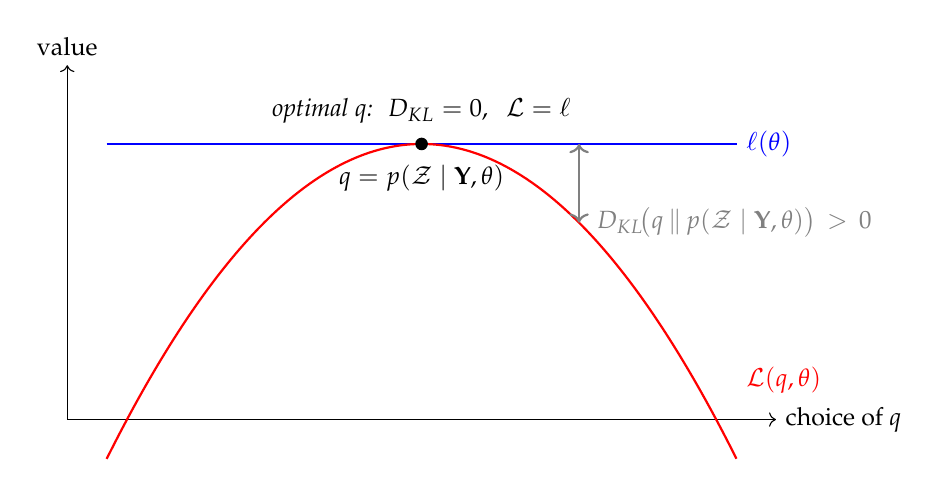
\begin{tikzpicture}[scale=1.0]
    % Axes
    \draw[->] (0,0) -- (9,0) node[right] {\small choice of $q$};
    \draw[->] (0,0) -- (0,4.5) node[above] {\small value};

    % Log-likelihood (constant horizontal line)
    \draw[thick, blue] (0.5,3.5) -- (8.5,3.5);
    \node[blue, right] at (8.5, 3.5) {\small $\ell(\theta)$};

    % ELBO (concave curve, tangent to ell at one point)
    \draw[thick, red, smooth, samples=100, domain=0.5:8.5]
        plot (\x, {3.5 - 0.25*(\x-4.5)^2});
    \node[red, right] at (8.5, 0.5) {\small $\mathcal{L}(q, \theta)$};

    % Gap = KL divergence (at a generic q)
    \draw[<->, thick, gray] (6.5, 3.5) -- (6.5, {3.5 - 0.25*(6.5-4.5)^2});
    \node[gray, right] at (6.6, 2.5) {\small $D_{KL}\!\big(q \,\|\, p(\mathcal{Z}\mid\mY,\theta)\big) \,>\, 0$};

    % Tangent point: optimal q = posterior
    \fill[black] (4.5, 3.5) circle (0.08);
    \node[above=4pt] at (4.5, 3.5) {\small \emph{optimal $q$:} $\;D_{KL} = 0,\;\; \mathcal{L} = \ell$};
    \node[below=4pt] at (4.5, 3.5) {\small $q = p(\mathcal{Z}\mid\mY,\theta)$};
\end{tikzpicture}
\caption{The ELBO as a function of $q$, at fixed $\theta$. The
log-likelihood $\ell(\theta)$ is a horizontal line (independent of
$q$); the ELBO $\mathcal{L}(q, \theta)$ is bounded above by $\ell$,
with vertical gap equal to $D_{KL}(q \,\|\, p(\mathcal{Z} \mid \mY, \theta))$.
The bound is tight at the optimal choice $q = p(\mathcal{Z} \mid \mY, \theta)$,
where the KL gap is zero and the ELBO coincides with the
log-likelihood.}
\label{fig:elbo-gap}
\end{figure}

\noindent
This is the geometry of the E-step: \emph{at fixed $\theta$, choose $q$
to push the ELBO up against the log-likelihood as much as possible.}
The M-step then exploits this by maximising the (now tight) ELBO over
$\theta$, which is equivalent to maximising the log-likelihood itself
at the current $q$. Iterating between these two moves is the EM
algorithm.

The upshot is that we are no longer fumbling in the dark when we choose
$q$. The ELBO itself, through its decomposition
\eqref{eq:elbo-decomposition}, tells us what the optimal $q$ is.

\newpage

\subsection{The Optimisation Problem and Alternating Maximisation}

We have set up a surrogate objective function $\mathcal{L}(q, \theta)$
that bounds the true log-likelihood from below and equals it at the
"right" $q$. The natural idea is to maximise $\mathcal{L}(q, \theta)$
in place of the intractable $\ell(\theta)$:
\[
\max_{q, \theta} \;\mathcal{L}(q, \theta).
\]
This is a joint maximisation in two "variables" — a distribution
$q(\mathcal{Z})$ and a parameter vector $\theta$. A simultaneous
optimisation over both is not feasible: the space of admissible
distributions $q$ is infinite-dimensional, and $\mathcal{L}$ is a
complicated non-convex function of $\theta$. We therefore resort to
\emph{alternating maximisation}, also known as \emph{coordinate
ascent}. In each iteration we hold one of the two arguments fixed and
maximise over the other:
\begin{enumerate}[leftmargin=1.5em, itemsep=3pt]
    \item \textbf{E-step}: fix $\theta$, maximise $\mathcal{L}(q, \theta)$ over $q$;
    \item \textbf{M-step}: fix $q$, maximise $\mathcal{L}(q, \theta)$ over $\theta$;
    \item Iterate until convergence.
\end{enumerate}
This yields a sequence of iterates $\theta^{(0)}, \theta^{(1)},
\theta^{(2)}, \ldots$, which — as we discuss at the end of this section —
is guaranteed to produce a monotonically non-decreasing sequence of
log-likelihood values.

Before moving on to the concrete derivations, it is worth spelling out
\emph{what each of these two steps does} in some detail, because the
roles of $q$ and $\theta$ and the meaning of "holding one fixed" become
very concrete once we look closely.

\subsubsection{The E-Step (Expectation Step)}
\label{subsec:e-step-preview}

Fix $\theta = \theta^{(j)}$, the current parameter estimate, and
maximise the ELBO with respect to the auxiliary distribution $q$:
\[
\max_q\;\mathcal{L}(q, \theta^{(j)})
\;=\; \mathbb{E}_q[\log p(\mY, \mathcal{Z} \mid \theta^{(j)})]
\;-\; \mathbb{E}_q[\log q(\mathcal{Z})].
\]
The decomposition \eqref{eq:elbo-decomposition} we derived in the
previous subsection gives us the answer immediately. Recall that
\[
\mathcal{L}(q, \theta^{(j)}) \;=\; \ell(\theta^{(j)})
\;-\; D_{KL}\!\big(q(\mathcal{Z})\,\|\,p(\mathcal{Z} \mid \mY, \theta^{(j)})\big).
\]
The first term is fixed (we have fixed $\theta^{(j)}$, so
$\ell(\theta^{(j)})$ is just a number). The second term is a non-negative
quantity that we subtract. Maximising $\mathcal{L}$ over $q$ therefore
amounts to \emph{minimising the KL divergence}, and the KL divergence is
zero \emph{if and only if} $q$ equals the posterior. Thus:
\begin{equation}
\boxed{\;\;q^{(j+1)}(\mathcal{Z}) \;=\; p\big(\mathcal{Z} \mid \mY, \theta^{(j)}\big).\;\;}
\label{eq:e-step-optimal-q}
\end{equation}
The optimal $q$ is the \emph{posterior distribution of the latent
variables given the observed data and the current parameters}. Not an
approximation, not a surrogate — the exact posterior.

\paragraph{What the E-step actually computes.}
Knowing that $q^{(j+1)} = p(\mathcal{Z} \mid \mY, \theta^{(j)})$
identifies the optimal $q$ but does not by itself give the M-step what
it needs.
The M-step, which will follow, needs to evaluate the ELBO
at this specific choice of $q$ in order to maximise it over $\theta$.
What does this require in practice?

The term in the ELBO that depends on $\theta$ is the expected
complete-data log-likelihood, which in our notation reads
\begin{equation}
L(\theta, \theta^{(j)}) \;\equiv\; \mathbb{E}_{q^{(j+1)}}\!\big[\log p(\mY, \mathcal{Z} \mid \theta)\big]
\;=\; \mathbb{E}_{\theta^{(j)}}\!\big[\log p(\mY, \mathcal{Z} \mid \theta) \,\big|\, \mY\big].
\label{eq:Q-function}
\end{equation}
We have used two equivalent notations: the first emphasises that the
expectation is taken under the distribution computed in the E-step; the
second — standard in the EM literature — emphasises that this is a
conditional expectation under $\theta^{(j)}$, given the observed data
$\mY$. We will use both interchangeably.

The complete-data log-likelihood $\log p(\mY, \mathcal{Z} \mid \theta)$ is
a sum of log-Gaussian and log-Gamma densities — in full detail, it will
contain terms such as:
\begin{itemize}[leftmargin=1.5em, itemsep=3pt]
    \item products involving the factors: $f_t$, $f_t f_t'$,
          $f_t f_{t-1}'$;
    \item scalar multiples of these factor products by the weights:
          $w^u_t \cdot f_t f_{t-1}'$, $w^\varepsilon_t \cdot f_t f_t'$,
          $w^\varepsilon_t \cdot y_t f_t'$;
    \item terms in the weights alone: $\log w^u_t$, $w^u_t$,
          $\log w^\varepsilon_t$, $w^\varepsilon_t$.
\end{itemize}
Since the latent quantities $\mathcal{Z}$ are unobserved, we cannot
evaluate these terms directly. But now we \emph{do} have a distribution
for $\mathcal{Z}$ — the posterior $q^{(j+1)}$ — and we can replace
every latent quantity by its \emph{expectation under $q^{(j+1)}$}. Taking
these expectations is precisely what the E-step does. Concretely, the
E-step produces the following summaries:

\medskip

\noindent\textbf{Smoothed factor moments:}
\begin{itemize}[leftmargin=1.5em, itemsep=2pt]
    \item $\hat{f}_{t \mid T}^{(j)} \equiv \mathbb{E}_{\theta^{(j)}}[f_t \mid \mY]$
          — smoothed factor means;
    \item $\mathbb{E}_{\theta^{(j)}}[f_t f_t' \mid \mY]$ — smoothed second
          moments;
    \item $\mathbb{E}_{\theta^{(j)}}[f_t f_{t-1}' \mid \mY]$ — smoothed
          cross-period second moments;
    \item $\mathbb{E}_{\theta^{(j)}}[f_{t-1} f_{t-1}' \mid \mY]$ — lagged
          second moments.
\end{itemize}

\noindent\textbf{Posterior weight expectations:}
\begin{itemize}[leftmargin=1.5em, itemsep=2pt]
    \item $\hat{w}^{u,(j)}_t \equiv \mathbb{E}_{\theta^{(j)}}[w^u_t \mid \mY]$ —
          posterior mean of the factor-side weight at time $t$;
    \item $\hat{w}^{\varepsilon,(j)}_t \equiv \mathbb{E}_{\theta^{(j)}}[w^\varepsilon_t \mid \mY]$ —
          posterior mean of the idiosyncratic-side weight at time $t$;
    \item $\mathbb{E}_{\theta^{(j)}}[\log w^u_t \mid \mY]$,
          $\mathbb{E}_{\theta^{(j)}}[\log w^\varepsilon_t \mid \mY]$ —
          posterior expected log-weights (needed for updating $\nu_u$
          and $\nu_\varepsilon$).
\end{itemize}

Once all of these quantities are computed, $L(\theta, \theta^{(j)})$ is a
fully explicit function of $\theta$ alone — every latent variable has
been replaced by a number — and is ready for the M-step.

\paragraph{How are these quantities actually computed?}
The computation naturally splits along the latent structure of the
model:
\begin{itemize}[leftmargin=1.5em, itemsep=3pt]
    \item The \emph{smoothed factor moments} are obtained via the
          \textbf{Kalman filter} (a forward recursion giving
          $p(f_t \mid y_1, \ldots, y_t, \theta^{(j)})$) followed by the
          \textbf{Kalman smoother} (a backward recursion giving
          $p(f_t \mid \mY, \theta^{(j)})$). The smoother is what lets us
          use future observations to sharpen our estimate of past
          factors. These recursions require, as inputs, the current
          $\theta^{(j)}$ and — crucially for our Student-$t$ setup — the
          posterior weight expectations as well.
    \item The \emph{posterior weight expectations} are obtained in
          closed form through the Gaussian–Gamma conjugacy previewed
          earlier: conditional on the data and the factors, the
          posterior of each $w$ is a Gamma distribution, whose mean can
          be written explicitly.
\end{itemize}

The two computations are coupled — the Kalman recursions need the
weights, the weight posteriors need the factors — and we resolve this
coupling by iterating within the E-step (an ECM inner loop), as
we shall see. 

\subsubsection{The M-Step (Maximisation Step)}
\label{subsec:m-step-preview}

Fix $q = q^{(j+1)}$, the posterior just computed in the E-step, and
maximise the ELBO with respect to the parameter vector $\theta$:
\[
\theta^{(j+1)} \;=\; \argmax_\theta\;\mathcal{L}(q^{(j+1)}, \theta).
\]
With $q$ held fixed, the ELBO simplifies considerably:
\[
\mathcal{L}(q^{(j+1)}, \theta)
\;=\; \underbrace{\mathbb{E}_{q^{(j+1)}}[\log p(\mY, \mathcal{Z} \mid \theta)]}_{\text{depends on } \theta}
\;-\; \underbrace{\mathbb{E}_{q^{(j+1)}}[\log q^{(j+1)}(\mathcal{Z})]}_{\text{does not depend on } \theta}.
\]
The second term is the (negative) entropy of $q^{(j+1)}$. Since
$q^{(j+1)}$ has been fixed in the E-step and does not depend on
$\theta$, the entire entropy term is a constant from the M-step's point
of view. Maximising $\mathcal{L}(q^{(j+1)}, \theta)$ over $\theta$ is
therefore equivalent to maximising just the first term, which is
precisely the expected complete-data log-likelihood $L(\theta,
\theta^{(j)})$ from \eqref{eq:Q-function}:
\begin{equation}
\boxed{\;\;\theta^{(j+1)} \;=\; \argmax_\theta\; L(\theta, \theta^{(j)})
\;=\; \argmax_\theta\; \mathbb{E}_{\theta^{(j)}}\!\big[\log p(\mY, \mathcal{Z} \mid \theta) \,\big|\, \mY\big].\;\;}
\label{eq:m-step-formulation}
\end{equation}

\paragraph{What are we actually maximising?}
The object $\log p(\mY, \mathcal{Z} \mid \theta)$ is the complete-data
log-likelihood — the log-likelihood we \emph{would} maximise if we had
observed $\mathcal{Z}$ alongside $\mY$. Under our DGP it is a sum of
simple log-Gaussian and log-Gamma densities, and in its raw form it is a
quadratic function of the factors $\mF$ (conditional on the weights
$W^u, W^\varepsilon$), plus linear-and-log terms in the weights. If we
could see $\mathcal{Z}$, maximising it over $\theta$ would be a
textbook exercise in closed-form OLS-type formulas.

But we cannot see $\mathcal{Z}$. What the M-step does instead is
maximise the \emph{expectation} of this complete-data log-likelihood
under the posterior $q^{(j+1)}$: it maximises the "average
log-likelihood", averaged over all possible paths of $\mathcal{Z}$,
weighted by how likely each path is given the data and $\theta^{(j)}$.

\paragraph{Why is this easier than the original problem?}
The crucial simplification is that \emph{the expectation has turned every
latent quantity into a fixed number}. Wherever the complete-data
log-likelihood contained a term like $f_t f_{t-1}'$ or
$w^\varepsilon_t \cdot y_t f_t'$, that term has been replaced by its
posterior expectation — a concrete scalar or matrix computed in the
E-step. Once this substitution is made, the object we maximise in the
M-step is a function of $\theta$ \emph{alone}, with no latent variables
left inside. It is a clean, finite-dimensional optimisation problem.

Better still: the dependence of this function on $\theta$ is exactly the
same as the dependence of a Gaussian log-likelihood on its parameters,
modulo the presence of the posterior weights as multiplicative
scaling factors. As a consequence, the M-step will yield
\emph{closed-form} updates for $\mL$, $\mA$, $\mQ$, $\mR$ — the same
OLS-type formulas as in the Gaussian DFM, but with sums over $t$
weighted by the posterior expectations $\hat{w}^u_t$ and
$\hat{w}^\varepsilon_t$. Only the updates for the degrees of freedom
$\nu_u$ and $\nu_\varepsilon$ will require a one-dimensional numerical
root-finding step (they have no closed-form maximiser due to the digamma
function arising in the Gamma log-density). We defer all of this later.

\paragraph{Intuition behind the M-step.}
The M-step answers a transparent question:

\begin{quote}
\emph{"Given that the latent variables $\mathcal{Z}$ were distributed as
$q^{(j+1)}$, which $\theta$ makes the observed data $\mY$ most likely?"}
\end{quote}

It is as if we had \emph{observed} the latent variables — but with their
specific unknown values replaced by their expected values under our best
current guess of their distribution. This is what makes EM tractable:
we are alternating between (i) "filling in" the latent variables with
their best current guess (E-step), and (ii) estimating $\theta$ as if
we had seen the filled-in values (M-step).

\subsubsection{Summary: E-Step and M-Step Side by Side}

The two steps are summarised in Table~\ref{tab:em-summary}.

\begin{table}[h!]
\centering
\small
\renewcommand{\arraystretch}{1.1}
\begin{tabular}{@{}p{1.5cm} p{2.7cm} p{2.2cm} p{8cm}@{}}
\toprule
\textbf{Step} & \textbf{Fixed} & \textbf{Optimised} & \textbf{Output} \\
\midrule
\textbf{E-step}
  & $\theta = \theta^{(j)}$
  & $q(\mathcal{Z})$
  & $q^{(j+1)} = p(\mathcal{Z} \mid \mY, \theta^{(j)})$ \\
  & & & \emph{Via:} Kalman filter/smoother (factor moments); Gaussian–Gamma conjugacy (weight expectations). \\
\addlinespace[2pt]
\textbf{M-step}
  & $q = q^{(j+1)}$
  & $\theta$
  & $\theta^{(j+1)} = \argmax_\theta\, \mathbb{E}_{q^{(j+1)}}[\log p(\mY, \mathcal{Z} \mid \theta)]$ \\
  & & & \emph{Via:} closed-form weighted-OLS for $\mL, \mA, \mQ, \mR$; numerical root-finding for $\nu_u, \nu_\varepsilon$. \\
\bottomrule
\end{tabular}
\caption{Structure of the EM algorithm for the Student-$t$ DFM.
E-step and M-step alternate, each holding one argument of the ELBO
fixed and maximising over the other.}
\label{tab:em-summary}
\end{table}

\bigskip


\paragraph{Monotonicity and convergence.}
Each EM iteration increases the ELBO (or leaves it unchanged). This is
easy to see: the E-step maximises $\mathcal{L}$ over $q$ with $\theta$
fixed, so $\mathcal{L}(q^{(j+1)}, \theta^{(j)}) \geq
\mathcal{L}(q^{(j)}, \theta^{(j)})$; the M-step maximises $\mathcal{L}$
over $\theta$ with $q$ fixed, so $\mathcal{L}(q^{(j+1)}, \theta^{(j+1)})
\geq \mathcal{L}(q^{(j+1)}, \theta^{(j)})$. Chaining the two,
\[
\mathcal{L}(q^{(j+1)}, \theta^{(j+1)}) \;\geq\; \mathcal{L}(q^{(j)}, \theta^{(j)}).
\]
Moreover, by the ELBO decomposition \eqref{eq:elbo-decomposition},
\emph{after the E-step} we have $\mathcal{L}(q^{(j+1)}, \theta^{(j)}) =
\ell(\theta^{(j)})$ (the KL gap is zero). Combining these two facts, one
can show that the log-likelihood itself is monotonically
non-decreasing:
\[
\ell(\theta^{(j+1)}) \;\geq\; \ell(\theta^{(j)}).
\]
This is the crucial property that makes EM a valid algorithm: although
we never compute $\ell(\theta)$ directly and never maximise it directly,
the values $\ell(\theta^{(0)}), \ell(\theta^{(1)}), \ldots$ form a
monotone sequence, and under mild regularity conditions they converge
to a (local) maximum of the likelihood.

\paragraph{A geometric reading of the iteration.}
The argument we have just given admits a useful visual interpretation,
illustrated in Figure~\ref{fig:em-iteration}. The blue curve is the
true log-likelihood $\ell(\theta)$ — the object we want to maximise
but cannot evaluate directly. At the start of iteration $j$, the
E-step constructs a lower bound (the red curve), tangent to
$\ell(\theta)$ at the current parameter value $\theta^{(j)}$: the
tangency reflects the fact that, after the E-step, the KL gap is
zero. The M-step then maximises this tangent lower bound, producing
$\theta^{(j+1)}$. At the new parameter value, $\ell$ is necessarily
at least as high as the maximum of the tangent bound, which in turn
is at least as high as $\ell(\theta^{(j)})$. Iterating, the EM
algorithm climbs the log-likelihood through a sequence of
\emph{tangent surrogate maximisations}.

\begin{figure}[h!]
\centering
\begin{tikzpicture}[scale=1.0]
    % Axes
    \draw[->] (0,0) -- (10.5,0) node[right] {\small $\theta$};
    \draw[->] (0,0) -- (0,5) node[above] {\small value};

    % Log-likelihood: a smooth concave curve
    \draw[thick, blue, smooth, samples=100, domain=0.5:10]
        plot (\x, {4.2 - 0.05*(\x-7)^2 - 0.4*exp(-0.5*(\x-2)^2)});
    \node[blue, right] at (10, {4.2 - 0.05*(10-7)^2}) {\small $\ell(\theta)$};

    % --- Helper: log-likelihood evaluated at theta values ---
    % Iteration 0: tangent at theta^{(0)} = 1.5
    \draw[thick, red!80, smooth, samples=80, domain=0.5:3.0]
        plot (\x, {2.36 - 0.6*(\x-1.5)^2});
    \fill[black] (1.5, 2.36) circle (0.07);
    \draw[dashed, gray] (1.5, 0) -- (1.5, 2.36);
    \node[below] at (1.5, 0) {\small $\theta^{(0)}$};

    % Iteration 1: tangent at theta^{(1)} = 4
    \draw[thick, red!80, smooth, samples=80, domain=2.8:5.5]
        plot (\x, {3.75 - 0.4*(\x-4)^2});
    \fill[black] (4, 3.75) circle (0.07);
    \draw[dashed, gray] (4, 0) -- (4, 3.75);
    \node[below] at (4, 0) {\small $\theta^{(1)}$};

    % Iteration 2: tangent at theta^{(2)} = 6.5
    \draw[thick, red!80, smooth, samples=80, domain=5.3:8.0]
        plot (\x, {4.19 - 0.4*(\x-6.5)^2});
    \fill[black] (6.5, 4.19) circle (0.07);
    \draw[dashed, gray] (6.5, 0) -- (6.5, 4.19);
    \node[below] at (6.5, 0) {\small $\theta^{(2)}$};

    \node[red!80, above right] at (5.6, 4.3) {\small ELBO at iter.\ $j$};

\end{tikzpicture}
\caption{Geometric reading of the EM algorithm. The blue curve is the
log-likelihood $\ell(\theta)$. At each iteration, the E-step
constructs a tangent lower bound (red), maximising which yields the
next parameter estimate. The procedure climbs the log-likelihood
through a sequence of tangent surrogate maximisations.}
\label{fig:em-iteration}
\end{figure}


\paragraph{The Bańbura–Modugno perspective.}
It is worth noting that the logic we have just followed — ELBO, Jensen's
inequality, alternating maximisation — is the "variational" view of EM,
popular in the machine-learning literature. The econometric tradition
following Bańbura and Modugno (2014) presents EM more directly: one
simply \emph{defines} the objective
$L(\theta, \theta^{(j)}) = \mathbb{E}_{\theta^{(j)}}[\log p(\mY, \mathcal{Z} \mid \theta) \mid \mY]$
and iterates: compute the expectation under $\theta^{(j)}$ (E-step),
maximise over $\theta$ (M-step). The two perspectives are mathematically
equivalent — as we have shown, the ELBO equals
$L(\theta, \theta^{(j)})$ up to a constant once $q$ is chosen as the
posterior — but the variational derivation has the pedagogical
advantage of making the role of $q$, the meaning of the bound, and the
reason for monotonic convergence fully transparent.

\newpage

\section{Deriving the Complete-Data Log-Likelihood}
\label{sec:complete-loglik}

\subsection{Setup and Notation}

We now assemble the \emph{complete-data log-likelihood} — the object the
M-step will maximise once the expectation over the latent variables has
been taken. Because the model has more latent structure than the Gaussian
DFM, this section is longer than its Gaussian counterpart. Every
intermediate step is made explicit.

Recall the full hierarchical system introduced before:
\begin{align*}
&\textbf{State:}\quad
    && f_t \;=\; \mA\, f_{t-1} \;+\; u_t,
    && u_t \mid w^u_t \sim \mathcal{N}\!\big(0,\; \mQ / w^u_t\big),
    && w^u_t \overset{iid}{\sim} \mathrm{Gamma}(\tfrac{\nu_u}{2}, \tfrac{\nu_u}{2}), \\
&\textbf{Observation:}\quad
    && y_t \;=\; \mL\, f_t \;+\; \varepsilon_t,
    && \varepsilon_t \mid w^\varepsilon_t \sim \mathcal{N}\!\big(0,\; \mR / w^\varepsilon_t\big),
    && w^\varepsilon_t \overset{iid}{\sim} \mathrm{Gamma}(\tfrac{\nu_\varepsilon}{2}, \tfrac{\nu_\varepsilon}{2}),
\end{align*}
with initial state $f_0 \sim \mathcal{N}(0, \boldsymbol{\Sigma}_0)$. 

We can also collect the system in compact matrix form. Stacking columns
across time:
\[
\underbrace{\mY}_{M \times T} \;=\; \mL\,\underbrace{\mF}_{r \times T} \;+\; \underbrace{\mE}_{M \times T},
\qquad
\underbrace{\mF}_{r \times T} \;=\; \mA\,\underbrace{\mF_{-1}}_{r \times T} \;+\; \underbrace{\mathbf{U}}_{r \times T},
\]


We recall the notation fixed so far:
\begin{itemize}[leftmargin=1.5em, itemsep=2pt]
    \item $\mY = [y_1 \mid \cdots \mid y_T] \in \mathbb{R}^{M \times T}$ — the observed data matrix;
    \item $\mF = [f_1 \mid \cdots \mid f_T] \in \mathbb{R}^{r \times (T+1)}$ — the full latent factor path;
    \item $\mF_{-1} = [f_0 \mid f_1 \mid \cdots \mid f_{T-1}] \in \mathbb{R}^{r \times T}$ — the lagged factor matrix (one-period shift of $\mF$);
    \item $W^u = [w^u_1, \ldots, w^u_T] \in \mathbb{R}^{T}_{>0}$ — latent weights on the factor side;
    \item $W^\varepsilon = [w^\varepsilon_1, \ldots, w^\varepsilon_T] \in \mathbb{R}^{T}_{>0}$ — latent weights on the idiosyncratic side;
    \item $\theta = \{\mL,\; \mA,\; \mQ,\; \mR,\; \nu_u,\; \nu_\varepsilon\}$ — parameter vector;
    \item $\mathcal{Z} = (\mF, W^u, W^\varepsilon)$ — the full latent triple.
\end{itemize}
The object we want to compute is
\[
\ell_c(\theta) \;=\; \log p\big(\mY, \mF, W^u, W^\varepsilon \mid \theta\big).
\]

\paragraph{Working assumption: complete data.}
Throughout this section we assume that the data matrix $\mY$ is fully
observed (no missing entries). This assumption simplifies the
exposition and lets us focus on the structural ingredients of the
complete-data log-likelihood. With missing data, only Block A is
formally affected — the observation equation is restricted to the
observed entries via a selection matrix $\mathbf{W}_t$ — but this
modification propagates through the Kalman filter, the weight update,
and the row-by-row M-step formulas for $\mL$ and $\mR$. The full
treatment deferred in another section.

\subsection{Factoring the Joint Distribution}

Using the product rule of probability, the joint density factorises
into five conditional blocks, one per DGP equation:
\begin{align*}
p\big(\mY, \mF, W^u, W^\varepsilon \mid \theta\big)
\;=\;
&\underbrace{\phantom{\big|}\, p(\mY \mid \mF, W^\varepsilon, \theta)\,\phantom{\big|}}_{\text{Block A: observation}}
\cdot
\underbrace{\phantom{\big|}\, p(\mF \mid W^u, \theta)\,\phantom{\big|}}_{\text{Blocks B and C: transitions + initial state}} \\[6pt]
&\;\cdot\;
\underbrace{\phantom{\big|}\, p(W^u \mid \theta)\,\phantom{\big|}}_{\text{Block D: Gamma prior on $W^u$}}
\;\cdot\;
\underbrace{\phantom{\big|}\, p(W^\varepsilon \mid \theta)\,\phantom{\big|}}_{\text{Block E: Gamma prior on $W^\varepsilon$}}.
\end{align*}
The factorisation reflects the causal structure of the DGP: nature
first draws the weights (which depend only on $\theta$, via the Gamma
priors), then draws the factors (whose conditional distribution given
$W^u$ and $\theta$ is Gaussian), then finally draws the observations
(Gaussian given the factors and $W^\varepsilon$). Below we work out each
block separately.

\paragraph{Block A — Observation density.}
Conditional on the factor $f_t$ and the idiosyncratic weight
$w^\varepsilon_t$, the observation $y_t$ is Gaussian:
\[
y_t \mid f_t, w^\varepsilon_t \;\sim\; \mathcal{N}\!\big(\mL f_t,\; \mR / w^\varepsilon_t\big).
\]
The mean $\mL f_t$ is the systematic component; the matrix
$\mR / w^\varepsilon_t$ is the \emph{conditional covariance matrix} of
$y_t$ given $f_t$ and $w^\varepsilon_t$. Note carefully: \emph{inside
the scale-mixture representation}, conditionally on the weight, this
matrix is a genuine covariance — the Gaussian $\mathcal{N}(\mL f_t, \mR/w^\varepsilon_t)$
has mean $\mL f_t$ and variance $\mR/w^\varepsilon_t$ in the usual
sense. The distinction between scale matrix and covariance matrix
emphasised before applies to the \emph{marginal}
distribution of $\varepsilon_t$ after integrating the weight out:
marginally, $\varepsilon_t \sim t(0, \mR, \nu_\varepsilon)$ and the
marginal covariance is $\tfrac{\nu_\varepsilon}{\nu_\varepsilon - 2}\mR$,
not $\mR$. Here, working within the hierarchical representation, we are
always in the conditional world and $\mR / w^\varepsilon_t$ is the
covariance matrix to be used.

A small realisation of $w^\varepsilon_t$ inflates the conditional
covariance and produces a diffuse Gaussian — the mechanism through
which heavy tails emerge when $w^\varepsilon_t$ is integrated out.
Conditional on $(\mF, W^\varepsilon)$, observations at different times
are independent, so
\[
p(\mY \mid \mF, W^\varepsilon, \theta) \;=\; \prod_{t=1}^{T} p(y_t \mid f_t, w^\varepsilon_t, \theta).
\]

\paragraph{Block B — Factor transition density.}
Conditional on the previous factor $f_{t-1}$ and the factor weight
$w^u_t$, the current factor is Gaussian:
\[
f_t \mid f_{t-1}, w^u_t \;\sim\; \mathcal{N}\!\big(\mA f_{t-1},\; \mQ / w^u_t\big).
\]
As in Block A, $\mQ / w^u_t$ is the \emph{conditional covariance
matrix} of $f_t$ within the hierarchical representation — not the scale
matrix. The scale matrix $\mQ$ appears instead in the marginal
distribution $u_t \sim t(0, \mQ, \nu_u)$, with marginal covariance
$\tfrac{\nu_u}{\nu_u - 2}\mQ$.

By the Markov property of the VAR(1) (conditional on the weights, $f_t$ depends on
the past only through $f_{t-1}$) and the chain rule,
\[
p(\mF \mid W^u, \theta) \;=\; p(f_0 \mid \theta)\, \prod_{t=1}^{T} p(f_t \mid f_{t-1}, w^u_t, \theta).
\]

\paragraph{Block C — Initial state density.}
The recursion requires a distribution for $f_0$; we adopt
\[
f_0 \sim \mathcal{N}(0, \boldsymbol{\Sigma}_0),
\]
with $\boldsymbol{\Sigma}_0$ the initial-state covariance. This block
is not weighted: $f_0$ pre-dates the dynamic system and is not touched
by the heavy-tailed innovations. As a consequence, the contribution of
Block C to the complete-data log-likelihood is identical to its
Gaussian counterpart, and its contribution to the M-step updates is
independent of $\nu_u$ and $\nu_\varepsilon$. 

\paragraph{Block D — Gamma prior on $W^u$.}
The factor-side weights are $iid$ Gamma across time:
\[
p(W^u \mid \theta) \;=\; \prod_{t=1}^{T} p(w^u_t \mid \theta),
\qquad
w^u_t \sim \mathrm{Gamma}(\tfrac{\nu_u}{2}, \tfrac{\nu_u}{2}).
\]
Note the dependence on $\theta$: this block contains $\nu_u$, and is the
only block — together with Block E — in which $\nu_u$ and
$\nu_\varepsilon$ appear. This fact will be crucial for the update of
the degrees of freedom in the M-step.

\paragraph{Block E — Gamma prior on $W^\varepsilon$.}
Analogously for the idiosyncratic side:
\[
p(W^\varepsilon \mid \theta) \;=\; \prod_{t=1}^{T} p(w^\varepsilon_t \mid \theta),
\qquad
w^\varepsilon_t \sim \mathrm{Gamma}(\tfrac{\nu_\varepsilon}{2}, \tfrac{\nu_\varepsilon}{2}).
\]

\subsection{Computing Each Block}

We now take the logarithm of each block, applying the multivariate
Gaussian log-density for Blocks A, B, C and the Gamma log-density for
Blocks D and E. For reference, the generic multivariate Gaussian
$X \sim \mathcal{N}(\mu, \Sigma)$ in $m$ dimensions has density
\[
p(x) \;=\; \frac{1}{(2\pi)^{m/2}\, |\Sigma|^{1/2}}
\exp\!\left(-\tfrac{1}{2}(x-\mu)'\Sigma^{-1}(x-\mu)\right),
\]
and log-density
\[
\log p(x) \;=\; -\tfrac{m}{2}\log(2\pi) - \tfrac{1}{2}\log|\Sigma|
- \tfrac{1}{2}(x-\mu)'\Sigma^{-1}(x-\mu).
\]
The three terms have a clear interpretation:
\begin{itemize}[leftmargin=1.5em, itemsep=2pt]
    \item $-\tfrac{m}{2}\log(2\pi)$: a normalising constant, depending
          only on the dimension $m$ — never on the parameters;
    \item $-\tfrac{1}{2}\log|\Sigma|$: penalises large determinants — a
          very spread-out distribution is penalised;
    \item $-\tfrac{1}{2}(x-\mu)'\Sigma^{-1}(x-\mu)$: penalises
          observations far from the mean $\mu$, in the Mahalanobis sense.
\end{itemize}
The generic $\mathrm{Gamma}(\alpha, \beta)$ with shape $\alpha > 0$ and
rate $\beta > 0$ has density
\[
p(w) \;=\; \frac{\beta^{\alpha}}{\Gamma(\alpha)}\, w^{\alpha-1}\, e^{-\beta w},
\qquad w > 0,
\]
and log-density
\[
\log p(w) \;=\; \alpha \log \beta - \log \Gamma(\alpha) + (\alpha - 1)\log w - \beta w.
\]

\paragraph{The complete-data log-likelihood as a sum.}
Taking the logarithm of the joint factorisation turns the product of
the five blocks into a sum of five log-densities:
\begin{align*}
\ell_c(\theta) \;&=\; \log p(\mY, \mF, W^u, W^\varepsilon \mid \theta) \\[4pt]
&=\; \underbrace{\log p(\mY \mid \mF, W^\varepsilon, \theta)}_{\text{Block A}}
\;+\; \underbrace{\log p(\mF \mid W^u, \theta)}_{\text{Blocks B and C}} \\[4pt]
&\quad\;+\; \underbrace{\log p(W^u \mid \theta)}_{\text{Block D}}
\;+\; \underbrace{\log p(W^\varepsilon \mid \theta)}_{\text{Block E}}.
\end{align*}
We now apply the log-density formulae above to each of the five blocks.


\subsubsection*{Block A — Observation Equation, $M$ Variables}

We have $y_t \mid f_t, w^\varepsilon_t \sim \mathcal{N}(\mL f_t,\, \mR/w^\varepsilon_t)$
where:
\begin{itemize}[leftmargin=1.5em, itemsep=2pt]
    \item $y_t$ is $M \times 1$, so $m = M$;
    \item the mean is $\mu = \mL f_t$ ($M \times 1$);
    \item the conditional covariance is $\Sigma = \mR/w^\varepsilon_t$
          ($M \times M$, diagonal, scaled by the weight. 
          Note that the diagonality of $\mR$ is preserved by the weighting:
          $\mR/w^\varepsilon_t$ is also diagonal for every $t$, with diagonal
          entries $r_i/w^\varepsilon_t$ for $i = 1, \ldots, M$. The inverse
          $(\mR/w^\varepsilon_t)^{-1}$ is therefore obtained simply as
          $\mathrm{diag}(w^\varepsilon_t/r_1, \ldots, w^\varepsilon_t/r_M)$.
          This sparsity pattern propagates through the entire algorithm: each
          M-step update preserves $\mR$ diagonal by construction, with no
          constraint being imposed during optimisation).
\end{itemize}

\paragraph{Plug into the multivariate normal formula.}
\[
p(y_t \mid f_t, w^\varepsilon_t, \theta)
\;=\; \frac{1}{(2\pi)^{M/2}\, \big|\mR/w^\varepsilon_t\big|^{1/2}}
\exp\!\left(-\tfrac{1}{2}(y_t - \mL f_t)'\,(\mR/w^\varepsilon_t)^{-1}\,(y_t - \mL f_t)\right).
\]

\paragraph{Taking logs.}
\[
\log p(y_t \mid f_t, w^\varepsilon_t, \theta)
\;=\; -\tfrac{M}{2}\log(2\pi) \;-\; \tfrac{1}{2}\log\!\big|\mR/w^\varepsilon_t\big|
\;-\; \tfrac{1}{2}(y_t - \mL f_t)'\,(\mR/w^\varepsilon_t)^{-1}\,(y_t - \mL f_t).
\]

\paragraph{Simplify the weight-dependent pieces.}
Two identities from linear algebra allow us to isolate the weight. For
the log-determinant,
\[
\log\!\big|\mR/w^\varepsilon_t\big|
\;=\; \log\!\big|(w^\varepsilon_t)^{-1}\,\mR\big|
\;=\; -M \log w^\varepsilon_t \;+\; \log|\mR|,
\]
where we used $|c \cdot A| = c^m\, |A|$ for a scalar $c$ and an
$m \times m$ matrix $A$. For the inverse,
\[
(\mR/w^\varepsilon_t)^{-1} \;=\; w^\varepsilon_t \cdot \mR^{-1}.
\]
Substituting both into the log-density:
\[
\log p(y_t \mid f_t, w^\varepsilon_t, \theta)
\;=\; -\tfrac{M}{2}\log(2\pi) \;+\; \tfrac{M}{2}\log w^\varepsilon_t \;-\; \tfrac{1}{2}\log|\mR|
\;-\; \tfrac{w^\varepsilon_t}{2}\,(y_t - \mL f_t)'\mR^{-1}(y_t - \mL f_t).
\]
The weight has come out in two places: as an additive term
$+\tfrac{M}{2}\log w^\varepsilon_t$ (from the log-determinant) and as a
multiplicative factor on the Mahalanobis quadratic form.

\paragraph{Sum over $t = 1, \ldots, T$.}
By conditional independence over time given $(\mF, W^\varepsilon)$,
\[
\log p(\mY \mid \mF, W^\varepsilon, \theta)
\;=\; \sum_{t=1}^{T} \log p(y_t \mid f_t, w^\varepsilon_t, \theta).
\]
Expanding the sum:
\begin{align*}
&= \sum_{t=1}^{T} \left[\, -\tfrac{M}{2}\log(2\pi)
\;+\; \tfrac{M}{2}\log w^\varepsilon_t
\;-\; \tfrac{1}{2}\log|\mR|
\;-\; \tfrac{w^\varepsilon_t}{2}(y_t - \mL f_t)'\mR^{-1}(y_t - \mL f_t) \,\right] \\[4pt]
&= -\tfrac{TM}{2}\log(2\pi)
\;+\; \tfrac{M}{2}\sum_{t=1}^{T} \log w^\varepsilon_t
\;-\; \tfrac{T}{2}\log|\mR|
\;-\; \tfrac{1}{2}\sum_{t=1}^{T} w^\varepsilon_t\,(y_t - \mL f_t)'\mR^{-1}(y_t - \mL f_t).
\end{align*}

\paragraph{Drop the constant and box the result.}
The term $-\tfrac{TM}{2}\log(2\pi)$ does not depend on any parameter in
$\theta$ nor on any latent variable, so we drop it:
\begin{equation}
\boxed{\,
\text{Block A} \;=\;
-\,\tfrac{T}{2}\log|\mR|
\;+\; \tfrac{M}{2}\sum_{t=1}^{T} \log w^\varepsilon_t
\;-\; \tfrac{1}{2}\sum_{t=1}^{T} w^\varepsilon_t\, (y_t - \mL f_t)'\mR^{-1}(y_t - \mL f_t) \;+\; \text{const}.
\,}
\label{eq:block-A}
\end{equation}

Three observations are worth making on \eqref{eq:block-A}:
\begin{itemize}[leftmargin=1.5em, itemsep=3pt]
    \item The determinant term $-\tfrac{T}{2}\log|\mR|$ is identical to
          the Gaussian case — it penalises a large idiosyncratic scale
          matrix.
    \item The new term $+\tfrac{M}{2}\sum_t \log w^\varepsilon_t$
          contains only the weights, not the structural parameters, and
          will contribute to the update of $\nu_\varepsilon$ together
          with the corresponding term in Block E.
    \item The Mahalanobis quadratic is now \emph{weighted} by
          $w^\varepsilon_t$. This is the technical origin of the
          ``weighted OLS'' structure of the M-step: observations at
          time periods with small $w^\varepsilon_t$ (extreme $y_t$'s,
          in the sense of the model) contribute less to the parameter
          updates. Robustness emerges automatically.
\end{itemize}

\subsubsection*{Block B — Factor Transition Equation, $r$ Factors}

We have $f_t \mid f_{t-1}, w^u_t \sim \mathcal{N}(\mA f_{t-1},\, \mQ/w^u_t)$
where:
\begin{itemize}[leftmargin=1.5em, itemsep=2pt]
    \item $f_t$ is $r \times 1$, so $m = r$;
    \item the mean is $\mu = \mA f_{t-1}$ ($r \times 1$);
    \item the conditional covariance is $\Sigma = \mQ/w^u_t$
          ($r \times r$, not necessarily diagonal, scaled by the weight).
\end{itemize}

\paragraph{Plug into the multivariate normal formula.}
\[
p(f_t \mid f_{t-1}, w^u_t, \theta)
\;=\; \frac{1}{(2\pi)^{r/2}\, \big|\mQ/w^u_t\big|^{1/2}}
\exp\!\left(-\tfrac{1}{2}(f_t - \mA f_{t-1})'\,(\mQ/w^u_t)^{-1}\,(f_t - \mA f_{t-1})\right).
\]

\paragraph{Taking logs.}
\[
\log p(f_t \mid f_{t-1}, w^u_t, \theta)
\;=\; -\tfrac{r}{2}\log(2\pi) \;-\; \tfrac{1}{2}\log\!\big|\mQ/w^u_t\big|
\;-\; \tfrac{1}{2}(f_t - \mA f_{t-1})'\,(\mQ/w^u_t)^{-1}\,(f_t - \mA f_{t-1}).
\]

\paragraph{Simplify the weight-dependent pieces.}
Exactly as in Block A, $|\mQ/w^u_t| = (w^u_t)^{-r}\,|\mQ|$, so
$\log|\mQ/w^u_t| = -r \log w^u_t + \log|\mQ|$, and
$(\mQ/w^u_t)^{-1} = w^u_t\,\mQ^{-1}$. Substituting:
\[
\log p(f_t \mid f_{t-1}, w^u_t, \theta)
\;=\; -\tfrac{r}{2}\log(2\pi) \;+\; \tfrac{r}{2}\log w^u_t \;-\; \tfrac{1}{2}\log|\mQ|
\;-\; \tfrac{w^u_t}{2}(f_t - \mA f_{t-1})'\mQ^{-1}(f_t - \mA f_{t-1}).
\]



\paragraph{Sum over $t = 1, \ldots, T$.}
By the Markov property (conditional on $(\mF_{-1}, W^u)$, each transition
is independent):
\[
\log p(\mF \mid \mF_{-1}, W^u, \theta)
\;=\; \sum_{t=1}^{T} \log p(f_t \mid f_{t-1}, w^u_t, \theta).
\]
Expanding the sum:
\begin{align*}
&= \sum_{t=1}^{T} \left[\, -\tfrac{r}{2}\log(2\pi)
\;+\; \tfrac{r}{2}\log w^u_t
\;-\; \tfrac{1}{2}\log|\mQ|
\;-\; \tfrac{w^u_t}{2}(f_t - \mA f_{t-1})'\mQ^{-1}(f_t - \mA f_{t-1}) \,\right] \\[4pt]
&= -\tfrac{Tr}{2}\log(2\pi)
\;+\; \tfrac{r}{2}\sum_{t=1}^{T} \log w^u_t
\;-\; \tfrac{T}{2}\log|\mQ|
\;-\; \tfrac{1}{2}\sum_{t=1}^{T} w^u_t\,(f_t - \mA f_{t-1})'\mQ^{-1}(f_t - \mA f_{t-1}).
\end{align*}

\paragraph{Drop the constant and box the result.}
\begin{equation}
\boxed{\,
\text{Block B} \;=\;
-\,\tfrac{T}{2}\log|\mQ|
\;+\; \tfrac{r}{2}\sum_{t=1}^{T} \log w^u_t
\;-\; \tfrac{1}{2}\sum_{t=1}^{T} w^u_t\, (f_t - \mA f_{t-1})'\mQ^{-1}(f_t - \mA f_{t-1}) \;+\; \text{const}.
\,}
\label{eq:block-B}
\end{equation}
The structural parallel with Block A is perfect: a determinant penalty
on $\mQ$, a linear-in-$\log w^u_t$ term contributing to the $\nu_u$
update, and a quadratic form weighted by $w^u_t$.

\subsubsection*{Block C — Initial State, $r$ Factors}

We specify $f_0 \sim \mathcal{N}(0, \boldsymbol{\Sigma}_0)$ where:
\begin{itemize}[leftmargin=1.5em, itemsep=2pt]
    \item $f_0$ is $r \times 1$, so $m = r$;
    \item the mean is $\mu = 0$;
    \item the covariance is $\boldsymbol{\Sigma}_0$ ($r \times r$).
\end{itemize}
This block is not weighted: the initial state pre-dates the dynamic
system and does not interact with the heavy-tailed innovations. It is
therefore structurally identical to the Gaussian case.

\paragraph{Plug into the formula.}
\[
p(f_0 \mid \theta) \;=\; \frac{1}{(2\pi)^{r/2}\, |\boldsymbol{\Sigma}_0|^{1/2}}
\exp\!\left(-\tfrac{1}{2}\, f_0'\,\boldsymbol{\Sigma}_0^{-1}\, f_0\right).
\]

\paragraph{Taking logs.}
\[
\log p(f_0 \mid \theta)
\;=\; -\tfrac{r}{2}\log(2\pi) \;-\; \tfrac{1}{2}\log|\boldsymbol{\Sigma}_0|
\;-\; \tfrac{1}{2}\, f_0'\,\boldsymbol{\Sigma}_0^{-1}\, f_0.
\]

\paragraph{Drop the constant and box.}
\begin{equation}
\boxed{\,
\text{Block C} \;=\;
-\,\tfrac{1}{2}\log|\boldsymbol{\Sigma}_0|
\;-\; \tfrac{1}{2}\,f_0'\,\boldsymbol{\Sigma}_0^{-1}\,f_0 \;+\; \text{const}.
\,}
\label{eq:block-C}
\end{equation}
Being a single density (one time period only, not a sum over $t$), this
block contributes a negligible amount to the log-likelihood when $T$ is
large. In practice, the role of Block C is mainly to initialise the
Kalman filter recursions; for $T \to \infty$ the parameter estimates
become independent of the initial condition.

\subsubsection*{Block D — Gamma Prior on $W^u$, $T$ Weights}

We specify $w^u_t \overset{iid}{\sim} \mathrm{Gamma}(\nu_u/2,\, \nu_u/2)$
where $\alpha = \beta = \nu_u/2$ for each $t$.

\paragraph{Plug into the Gamma formula.}
\[
p(w^u_t \mid \theta)
\;=\; \frac{(\nu_u/2)^{\nu_u/2}}{\Gamma(\nu_u/2)}\,
(w^u_t)^{\nu_u/2 - 1}\, e^{-(\nu_u/2)\, w^u_t},
\qquad w^u_t > 0.
\]

\paragraph{Taking logs.}
\[
\log p(w^u_t \mid \theta)
\;=\; \tfrac{\nu_u}{2}\log\!\tfrac{\nu_u}{2}
\;-\; \log \Gamma\!\big(\tfrac{\nu_u}{2}\big)
\;+\; \big(\tfrac{\nu_u}{2} - 1\big)\log w^u_t
\;-\; \tfrac{\nu_u}{2}\, w^u_t.
\]

\paragraph{Sum over $t = 1, \ldots, T$.}
By independence of the weights:
\begin{align*}
\log p(W^u \mid \theta)
&\;=\; \sum_{t=1}^{T} \log p(w^u_t \mid \theta) \\[4pt]
&\;=\; \sum_{t=1}^{T} \left[\, \tfrac{\nu_u}{2}\log\!\tfrac{\nu_u}{2}
\;-\; \log \Gamma\!\big(\tfrac{\nu_u}{2}\big)
\;+\; \big(\tfrac{\nu_u}{2} - 1\big)\log w^u_t
\;-\; \tfrac{\nu_u}{2}\, w^u_t \,\right] \\[4pt]
&\;=\; T\!\left[\,\tfrac{\nu_u}{2}\log\!\tfrac{\nu_u}{2}
                  \;-\; \log \Gamma\!\big(\tfrac{\nu_u}{2}\big)\,\right]
\;+\; \big(\tfrac{\nu_u}{2} - 1\big)\sum_{t=1}^{T} \log w^u_t
\;-\; \tfrac{\nu_u}{2} \sum_{t=1}^{T} w^u_t.
\end{align*}

\paragraph{Box the result.}
There is no additive constant to drop here: all terms depend either on
$\nu_u$ (the parameter) or on the latent weights.
\begin{equation}
\boxed{\,
\begin{aligned}
\text{Block D} \;=\;
& \;\; T \left[\, \tfrac{\nu_u}{2}\log\!\tfrac{\nu_u}{2}
            \;-\; \log \Gamma\!\big(\tfrac{\nu_u}{2}\big)\,\right] \\[3pt]
& \;+\; \big(\tfrac{\nu_u}{2} - 1\big)\sum_{t=1}^{T}\log w^u_t
\;-\; \tfrac{\nu_u}{2}\sum_{t=1}^{T} w^u_t.
\end{aligned}
\,}
\label{eq:block-D}
\end{equation}

The structure of Block D is important and worth anatomising in detail.
Three types of terms appear:
\begin{itemize}[leftmargin=1.5em, itemsep=3pt]
    \item A term depending on $\nu_u$ but \emph{not} on the weights:
          $T \big[\tfrac{\nu_u}{2}\log\tfrac{\nu_u}{2} - \log \Gamma(\tfrac{\nu_u}{2})\big]$.
          This term will be entirely responsible for the (lack of)
          closed-form update of $\nu_u$ in the M-step: the
          $\log \Gamma$ means that its derivative involves the
          \emph{digamma function} $\psi(\cdot)$, and setting the
          derivative to zero yields an implicit equation in $\nu_u$
          that must be solved numerically.
    \item A term linear in $\sum_t \log w^u_t$, multiplied by
          $(\nu_u/2 - 1)$. Taking the E-step expectation replaces
          $\log w^u_t$ by its posterior mean
          $\mathbb{E}[\log w^u_t \mid \mY, \theta^{(j)}]$, a quantity
          we will compute in closed form (Gaussian–Gamma conjugacy).
    \item A term linear in $\sum_t w^u_t$, multiplied by $-\nu_u/2$.
          Taking the E-step expectation replaces $w^u_t$ by
          $\hat{w}^{u,(j)}_t = \mathbb{E}[w^u_t \mid \mY, \theta^{(j)}]$.
\end{itemize}
Notice that Block D contains \emph{only} $\nu_u$ and the weights
$W^u$. It does not contain $\mL, \mA, \mQ, \mR$, nor any of the
idiosyncratic-side objects. This cleanly decouples the update of
$\nu_u$ from the updates of the other parameters in the M-step: when
maximising over $\mL, \mA, \mQ, \mR$, the entire Block D is an
irrelevant additive constant; when maximising over $\nu_u$, Blocks A,
B, C, and E are irrelevant constants (the weights in Blocks A and B,
once taken in expectation, do not depend on $\nu_u$ themselves).

\subsubsection*{Block E — Gamma Prior on $W^\varepsilon$, $T$ Weights}

By direct analogy with Block D, substituting $\nu_u \to \nu_\varepsilon$
and $w^u_t \to w^\varepsilon_t$.

\paragraph{Plug into the Gamma formula.}
\[
p(w^\varepsilon_t \mid \theta)
\;=\; \frac{(\nu_\varepsilon/2)^{\nu_\varepsilon/2}}{\Gamma(\nu_\varepsilon/2)}\,
(w^\varepsilon_t)^{\nu_\varepsilon/2 - 1}\, e^{-(\nu_\varepsilon/2)\, w^\varepsilon_t},
\qquad w^\varepsilon_t > 0.
\]

\paragraph{Take logs and sum.}
Going through the same algebra as Block D:
\begin{equation}
\boxed{\,
\begin{aligned}
\text{Block E} \;=\;
& \;\; T \left[\, \tfrac{\nu_\varepsilon}{2}\log\!\tfrac{\nu_\varepsilon}{2}
            \;-\; \log \Gamma\!\big(\tfrac{\nu_\varepsilon}{2}\big)\,\right] \\[3pt]
& \;+\; \big(\tfrac{\nu_\varepsilon}{2} - 1\big)\sum_{t=1}^{T}\log w^\varepsilon_t
\;-\; \tfrac{\nu_\varepsilon}{2}\sum_{t=1}^{T} w^\varepsilon_t.
\end{aligned}
\,}
\label{eq:block-E}
\end{equation}

All observations made about Block D transfer directly, with the
subscript $\varepsilon$ replacing $u$: the decoupling of
$\nu_\varepsilon$ from the structural parameters, the $\log \Gamma$
term implying numerical root-finding, and the linear dependence on
$\sum_t w^\varepsilon_t$ and $\sum_t \log w^\varepsilon_t$.

\subsection{The Trace Trick with Weights}

Before assembling the complete log-likelihood we recall a useful
identity. The \emph{trace} of a matrix $A$ is the sum of its diagonal
entries, $\mathrm{tr}(A) = \sum_i a_{ii}$. For any vector $x$ and
square matrix $M$,
\[
x'\, M\, x \;=\; \mathrm{tr}(M x x').
\]
This ``trace trick'' is useful for two reasons. First, the trace is a
linear operator, so it commutes with expectations:
\[
\mathbb{E}[x'M x] \;=\; \mathbb{E}[\mathrm{tr}(M x x')] \;=\; \mathrm{tr}(M\, \mathbb{E}[x x']).
\]
This will let us replace the latent outer product $xx'$ inside the
trace with its posterior expectation — exactly what the E-step needs.
Second, the trace is additive over sums, so
$\sum_t \mathrm{tr}(A_t) = \mathrm{tr}(\sum_t A_t)$.

\paragraph{Weighted case.}
In our setting, each summand in Blocks A and B is multiplied by a
scalar weight ($w^\varepsilon_t$ or $w^u_t$). Since scalars commute
with everything, the weighted version of the trace trick is:
\begin{align*}
\sum_{t=1}^{T} w^\varepsilon_t\, (y_t - \mL f_t)' \mR^{-1} (y_t - \mL f_t)
&\;=\; \mathrm{tr}\!\Bigg[\mR^{-1} \sum_{t=1}^{T} w^\varepsilon_t\, (y_t - \mL f_t)(y_t - \mL f_t)'\Bigg], \\[4pt]
\sum_{t=1}^{T} w^u_t\, (f_t - \mA f_{t-1})' \mQ^{-1} (f_t - \mA f_{t-1})
&\;=\; \mathrm{tr}\!\Bigg[\mQ^{-1} \sum_{t=1}^{T} w^u_t\, (f_t - \mA f_{t-1})(f_t - \mA f_{t-1})'\Bigg].
\end{align*}
The weights enter the sum of outer products and stay there. This is
the form of the quadratic terms we will use throughout the M-step.


\subsection{Complete-Data Log-Likelihood: Final Form}

Combining Blocks A through E, we obtain the full complete-data
log-likelihood. Using the weighted trace trick on the quadratic terms
in Blocks A and B, and dropping all additive constants independent of
$\theta$ and of the latent variables:
\begin{equation}
\boxed{\,
\begin{aligned}
\ell_c(\theta) \;=\;\;
&-\tfrac{1}{2}\log|\boldsymbol{\Sigma}_0| \;-\; \tfrac{1}{2}\,f_0'\,\boldsymbol{\Sigma}_0^{-1}\,f_0 \\[3pt]
&-\tfrac{T}{2}\log|\mQ|
\;+\; \tfrac{r}{2}\sum_{t=1}^{T} \log w^u_t
\;-\; \tfrac{1}{2}\,\mathrm{tr}\!\Bigg[\mQ^{-1}\sum_{t=1}^{T} w^u_t\, (f_t - \mA f_{t-1})(f_t - \mA f_{t-1})'\Bigg] \\[3pt]
&-\tfrac{T}{2}\log|\mR|
\;+\; \tfrac{M}{2}\sum_{t=1}^{T} \log w^\varepsilon_t
\;-\; \tfrac{1}{2}\,\mathrm{tr}\!\Bigg[\mR^{-1}\sum_{t=1}^{T} w^\varepsilon_t\, (y_t - \mL f_t)(y_t - \mL f_t)'\Bigg] \\[3pt]
&+\, T \left[\tfrac{\nu_u}{2}\log\!\tfrac{\nu_u}{2} \;-\; \log \Gamma\!\big(\tfrac{\nu_u}{2}\big)\right]
\;+\; \big(\tfrac{\nu_u}{2} - 1\big)\sum_{t=1}^{T}\log w^u_t
\;-\; \tfrac{\nu_u}{2}\sum_{t=1}^{T} w^u_t \\[3pt]
&+\, T \left[\tfrac{\nu_\varepsilon}{2}\log\!\tfrac{\nu_\varepsilon}{2} \;-\; \log \Gamma\!\big(\tfrac{\nu_\varepsilon}{2}\big)\right]
\;+\; \big(\tfrac{\nu_\varepsilon}{2} - 1\big)\sum_{t=1}^{T}\log w^\varepsilon_t
\;-\; \tfrac{\nu_\varepsilon}{2}\sum_{t=1}^{T} w^\varepsilon_t.
\end{aligned}
\,}
\label{eq:complete-loglik-final}
\end{equation}
This is the complete-data log-likelihood of the Student-$t$ DFM. It
contains five groups of terms: one from each of the five blocks A–E.
The Gaussian DFM is recovered as a limiting case: when
$\nu_u, \nu_\varepsilon \to \infty$, all weights collapse to
$w^u_t = w^\varepsilon_t = 1$, the
$\log w$ terms vanish, and the $\nu$-dependent terms in Blocks D and E
become constants that drop out — leaving exactly the Gaussian expression
familiar from the standard DFM.


\subsection{Identifying the Blocks of Parameters}

Before moving to the E-step, it is helpful to group the terms of
\eqref{eq:complete-loglik-final} by the parameter they depend on.
This decomposition will be directly reflected in the M-step, where we
will maximise each group separately.

\begin{center}
\renewcommand{\arraystretch}{1.4}
\begin{tabular}{@{}p{2.2cm} p{11.5cm}@{}}
\toprule
\textbf{Parameter} & \textbf{Relevant terms in $\ell_c(\theta)$} \\
\midrule
$\boldsymbol{\Sigma}_0$ & $-\tfrac{1}{2}\log|\boldsymbol{\Sigma}_0| - \tfrac{1}{2}f_0'\boldsymbol{\Sigma}_0^{-1}f_0$ (Block C) \\
$\mA$ & Quadratic in Block B: $-\tfrac{1}{2}\mathrm{tr}\!\big[\mQ^{-1}\sum_t w^u_t (f_t - \mA f_{t-1})(f_t - \mA f_{t-1})'\big]$ \\
$\mQ$ & Block B log-det and quadratic \\
$\mL$ & Quadratic in Block A: $-\tfrac{1}{2}\mathrm{tr}\!\big[\mR^{-1}\sum_t w^\varepsilon_t (y_t - \mL f_t)(y_t - \mL f_t)'\big]$ \\
$\mR$ & Block A log-det and quadratic \\
$\nu_u$ & Block D: $T\big[\tfrac{\nu_u}{2}\log\tfrac{\nu_u}{2} - \log\Gamma(\tfrac{\nu_u}{2})\big] + \tfrac{\nu_u}{2}\sum_t(\log w^u_t - w^u_t) - \sum_t \log w^u_t$ \\
$\nu_\varepsilon$ & Block E: $T\big[\tfrac{\nu_\varepsilon}{2}\log\tfrac{\nu_\varepsilon}{2} - \log\Gamma(\tfrac{\nu_\varepsilon}{2})\big] + \tfrac{\nu_\varepsilon}{2}\sum_t(\log w^\varepsilon_t - w^\varepsilon_t) - \sum_t \log w^\varepsilon_t$ \\
\bottomrule
\end{tabular}
\end{center}

Two features of this decomposition are worth stressing:

\begin{itemize}[leftmargin=1.5em, itemsep=3pt]
    \item The updates of $\mL$, $\mA$, $\mQ$, $\mR$ will be
          \emph{weighted OLS}: identical in structure to the Gaussian
          case, except that the sum over $t$ carries multiplicative
          factors $\hat{w}^\varepsilon_t$ or $\hat{w}^u_t$ — the
          posterior weight expectations from the E-step.
    \item The updates of $\nu_u, \nu_\varepsilon$ are entirely
          \emph{decoupled} from the other parameters. Blocks D and E
          contain only the degrees of freedom and the weights. As we
          shall see, the first-order conditions for $\nu$ involve the
          digamma function and therefore do not admit a closed form,
          requiring a numerical root-finding step. This is the ECME
          feature of the algorithm — expectation-conditional-maximisation
          extended.
\end{itemize}

\subsection{The Expected Complete-Data Log-Likelihood}

As established in the discussion of alternating maximisation, the M-step cannot directly maximise the complete-data log-likelihood $\ell_c(\theta)$ because it depends on the latent variables $\mathcal{Z} = \{\mF, W^u, W^\varepsilon\}$, which are not observed. To move forward, we must resolve this dependency by taking a conditional expectation.

We define our surrogate objective function, $\Xi(\theta \mid \theta^{(j)})$, as the expectation of the complete-data log-likelihood under the posterior distribution computed at the current parameter estimate $\theta^{(j)}$:
\begin{equation}
\Xi(\theta \mid \theta^{(j)}) \;\equiv\; \mathbb{E}_{\theta^{(j)}} \big[ \ell_c(\theta) \mid \mY \big].
\label{eq:Xi-function}
\end{equation}
By the linearity of the expectation operator, $\Xi(\theta \mid \theta^{(j)})$ is simply the sum of the expectations of the five blocks (A--E) identified in the previous section. Crucially, since $\ell_c(\theta)$ is a linear-in-parameters function of the latent quantities, the expectation operator can be pushed inside the summations. 

This transformation effectively ``linearises'' the latent structure: every unobserved term (whether a factor, a weight, or their product) is replaced by its best estimate given the available data. Maximising $\Xi$ is thus equivalent to performing a series of weighted regressions where the ``missing variables'' has been filled in by its posterior moments.

\begin{equation}
\boxed{\,
\small % Riduce leggermente la dimensione per farla rientrare
\begin{aligned}
\Xi(\theta \mid \theta^{(j)}) \;=\;\;
&-\tfrac{1}{2}\log|\boldsymbol{\Sigma}_0| \;-\; \tfrac{1}{2}\,\mathrm{tr}\big(\boldsymbol{\Sigma}_0^{-1} \mathbb{E}_{\theta^{(j)}}[f_0 f_0' \mid \mY]\big) \\[3pt]
&-\tfrac{T}{2}\log|\mQ| \;+\; \tfrac{r}{2}\sum_{t=1}^{T} \mathbb{E}_{\theta^{(j)}}[\log w^u_t \mid \mY] \\
&\quad - \tfrac{1}{2}\,\mathrm{tr}\!\Bigg[\mQ^{-1}\sum_{t=1}^{T} \mathbb{E}_{\theta^{(j)}}[w^u_t\, (f_t - \mA f_{t-1})(f_t - \mA f_{t-1})' \mid \mY]\Bigg] \\[3pt]
&-\tfrac{T}{2}\log|\mR| \;+\; \tfrac{M}{2}\sum_{t=1}^{T} \mathbb{E}_{\theta^{(j)}}[\log w^\varepsilon_t \mid \mY] \\
&\quad - \tfrac{1}{2}\,\mathrm{tr}\!\Bigg[\mR^{-1}\sum_{t=1}^{T} \mathbb{E}_{\theta^{(j)}}[w^\varepsilon_t\, (y_t - \mL f_t)(y_t - \mL f_t)' \mid \mY]\Bigg] \\[3pt]
&+\, T \left[\tfrac{\nu_u}{2}\log\!\tfrac{\nu_u}{2} \;-\; \log \Gamma\!\big(\tfrac{\nu_u}{2}\big)\right]
\;+\; \big(\tfrac{\nu_u}{2} - 1\big)\sum_{t=1}^{T}\mathbb{E}_{\theta^{(j)}}[\log w^u_t \mid \mY]
\;-\; \tfrac{\nu_u}{2}\sum_{t=1}^{T} \hat{w}^{u,(j)}_t \\[3pt]
&+\, T \left[\tfrac{\nu_\varepsilon}{2}\log\!\tfrac{\nu_\varepsilon}{2} \;-\; \log \Gamma\!\big(\tfrac{\nu_\varepsilon}{2}\big)\right]
\;+\; \big(\tfrac{\nu_\varepsilon}{2} - 1\big)\sum_{t=1}^{T}\mathbb{E}_{\theta^{(j)}}[\log w^\varepsilon_t \mid \mY]
\;-\; \tfrac{\nu_\varepsilon}{2}\sum_{t=1}^{T} \hat{w}^{\varepsilon,(j)}_t.
\end{aligned}
\,}
\label{eq:Xi-expanded}
\end{equation}

This expression clarifies the "step forward" mentioned earlier: every unobserved quantity has been replaced by a numerical summary produced by the E-step. Maximising $\Xi$ is now a deterministic optimisation problem where the parameters $\theta = \{\mA, \mL, \mQ, \mR, \nu_u, \nu_\varepsilon\}$ are the only variables.

\subsection{Preview of the E-Step}

We have just established that $\Xi(\theta \mid \theta^{(j)})$ requires
posterior expectations of every latent quantity appearing in
$\ell_c(\theta)$. Anticipating what the next section derives in
detail, we record here the list of objects the E-step must produce:

\begin{itemize}[leftmargin=1.5em, itemsep=3pt]
    \item \textbf{Factor moments}, for the Blocks A, B, C terms:
          $\mathbb{E}[f_t \mid \mY, \theta^{(j)}]$,
          $\mathbb{E}[f_t f_t' \mid \mY, \theta^{(j)}]$,
          $\mathbb{E}[f_t f_{t-1}' \mid \mY, \theta^{(j)}]$,
          $\mathbb{E}[f_0 f_0' \mid \mY, \theta^{(j)}]$.
    \item \textbf{Posterior weight means}, for the $w$-multiplied
          terms in Blocks A, B and the linear $w$ terms in Blocks D, E:
          $\hat{w}^{u,(j)}_t = \mathbb{E}[w^u_t \mid \mY, \theta^{(j)}]$ and
          $\hat{w}^{\varepsilon,(j)}_t = \mathbb{E}[w^\varepsilon_t \mid \mY, \theta^{(j)}]$.
    \item \textbf{Posterior log-weight means}, for the $\log w$ terms in
          Blocks A, B, D, E (needed essentially only for the $\nu$ updates):
          $\mathbb{E}[\log w^u_t \mid \mY, \theta^{(j)}]$ and
          $\mathbb{E}[\log w^\varepsilon_t \mid \mY, \theta^{(j)}]$.
    \item \textbf{Weighted cross-moments}, for the quadratic terms:
          $\mathbb{E}[w^\varepsilon_t\, f_t f_t' \mid \mY, \theta^{(j)}]$,
          $\mathbb{E}[w^u_t\, f_t f_t' \mid \mY, \theta^{(j)}]$,
          $\mathbb{E}[w^u_t\, f_t f_{t-1}' \mid \mY, \theta^{(j)}]$,
          $\mathbb{E}[w^u_t\, f_{t-1} f_{t-1}' \mid \mY, \theta^{(j)}]$.
\end{itemize}
The factor moments are obtained via the Kalman filter/smoother applied
to the conditionally Gaussian model (conditional on the weights). The
posterior weight quantities are obtained in closed form through the
Gaussian–Gamma conjugacy. The weighted cross-moments require care because they mix factors and 
weights—a property known as \emph{non-separability of expectations}. 
These are not simple products of marginal expectations because, in 
the posterior, the latent factors and the weights are conditional on 
the same data $\mY$ and thus become dependent. The treatment of 
these cross-moments is one of the subtler points of the derivation, 
and it is precisely what distinguishes the robust DFM from a 
standard Kalman filter with pre-determined weights.
These computations are the subject of the next section.
\newpage

\section{Initialisation of the EM Algorithm}
\label{sec:initialisation}

The EM algorithm is a local optimisation method: at every iteration it
increases the log-likelihood (weakly), but what it ultimately converges
to depends on the starting point $\theta^{(0)}$. A badly initialised EM
can converge to a sub-optimal local maximum, get stuck on the boundary
of the parameter space (for instance producing a near-singular scale
matrix), or converge extremely slowly. A good initialisation, by
contrast, often brings the algorithm to the vicinity of the global
maximum in just a handful of iterations.

For the standard Gaussian DFM, there is a well-established initialisation
strategy due to Bańbura and Modugno (2014): initialise the factors by
Principal Component Analysis (PCA), then estimate all other parameters
via ordinary least squares on the PCA factors. We extend this strategy
to the Student-$t$ DFM by adding two new ingredients: initial values
for the degrees-of-freedom parameters $\nu_u, \nu_\varepsilon$, and
initial values for the latent weights $W^u, W^\varepsilon$. A further
practical complication, addressed in this section, is that the
observation matrix $\mY$ typically contains missing entries — both at
the end of the sample (ragged edge from non-synchronous releases) and
within the sample (mixed-frequency variables observed only every third
period). Since PCA requires a complete data matrix, we describe how
$\mY$ is preliminarily completed before the PCA step, with the
caveat that this filled-in version is used \emph{only} for
initialisation: once the EM iterations begin, the model relies
exclusively on the selection-matrix framework
that we will see later and the imputed entries are discarded.

\subsection{Why Initialisation Matters}

The complete-data log-likelihood
\eqref{eq:complete-loglik-final} is not globally concave in $\theta$.
It has multiple local maxima, corresponding to different factor
orderings, factor sign choices (a factor is identified only up to a
sign), and — more substantively — to different allocations of variance
between the common and idiosyncratic components. The EM algorithm,
being a monotone ascent procedure, necessarily converges to \emph{some}
local maximum, but which one is determined entirely by $\theta^{(0)}$.

Moreover, the Student-$t$ extension enlarges the parameter space with
two additional parameters ($\nu_u, \nu_\varepsilon$) that are
notoriously difficult to estimate well. A poor initial value of $\nu$
can lead the algorithm either to collapse onto the Gaussian limit
($\nu \to \infty$) — wasting the heavy-tailed flexibility of the model —
or to a degenerate heavy-tailed regime ($\nu \to 0$) where a handful of
outliers dominate the likelihood. A sensible initialisation of $\nu_u$
and $\nu_\varepsilon$ is therefore at least as important as the
initialisation of the structural parameters.

\subsection{Initialising the Factors by PCA}

The strategy begins with a fact that is specific to factor models:
\emph{if} the factors were observed, estimating all other parameters
would reduce to standard regressions. So, the natural starting point is
to \emph{construct} an initial guess for the factors directly from the
data.

Principal Component Analysis provides exactly such a construction.
Given the standardised data matrix
$\tilde{\mY} \in \mathbb{R}^{M \times T}$ — where each row has been
centred and rescaled to unit variance — form the sample covariance
matrix
\[
\widehat{\boldsymbol{\Sigma}}_Y \;=\; \frac{1}{T}\,\tilde{\mY}\,\tilde{\mY}'
\;\in\; \mathbb{R}^{M \times M}.
\]
Let $v_1, \ldots, v_r \in \mathbb{R}^M$ be the eigenvectors of
$\widehat{\boldsymbol{\Sigma}}_Y$ corresponding to the $r$ largest
eigenvalues $\lambda_1 \geq \lambda_2 \geq \cdots \geq \lambda_r > 0$,
and collect them in the $M \times r$ matrix $V = [v_1 \mid \cdots \mid v_r]$.

The initial factor estimates are obtained by projecting the
standardised data onto the PCA directions:
\begin{equation}
\mF^{(0)} \;=\; V'\,\tilde{\mY} \;\in\; \mathbb{R}^{r \times T}.
\label{eq:init-F}
\end{equation}
That is, at time $t$, the $k$-th initial factor is
$f^{(0)}_{k,t} = v_k'\,\tilde{y}_t$, the inner product of the $k$-th
PCA direction with the standardised observation. The columns of
$\mF^{(0)}$ are the \emph{principal component scores} of the data.

Geometrically, the PCA factors are the directions of maximum variance
in the data — by construction they capture the largest share of the
co-movement across series, which is exactly what latent factors are
meant to represent. This is why PCA is such a natural starting point:
under mild regularity conditions, as $M, T \to \infty$, the PCA
estimator consistently recovers the true factor space (up to a
rotation). In finite samples it is a consistent but inefficient
estimator; the EM iterations will refine it.

\paragraph{Handling mixed frequencies and ragged edges.}
In the presence of mixed-frequency data and ragged edges, the sample 
covariance matrix $\widehat{\boldsymbol{\Sigma}}_Y$ cannot be computed 
directly because the panel is unbalanced. To address this we follow 
the broad logic of Giannone, Reichlin, and Small (2008) and Bańbura 
and Modugno (2014), performing PCA on a balanced version of the 
panel obtained by filling the missing entries in two distinct ways.

For quarterly series — which are structurally missing in non-quarter-end 
months — we disaggregate the quarterly observation into monthly 
values that satisfy the Mariano–Murasawa aggregation 
\eqref{eq:mm-aggregation}. Assuming locally constant monthly values 
within each quarter, we solve the Mariano–Murasawa restriction 
recursively across quarters, obtaining an implied monthly series 
that is consistent with the aggregation scheme adopted in the model. 
This is more principled than a simple linear interpolation, as it 
preserves the economic structure of the quarterly observation.

For generic missings arising from ragged-edge publication delays or
sample gaps, we fill with draws from a standard Gaussian
$\mathcal{N}(0, 1)$. This choice is consistent with the centred and
standardised data convention adopted at the beginning: each series
has empirical mean zero and empirical variance one by construction,
so unit-variance Gaussian draws are of the same scale as the observed
data. We are aware that this is a deliberate simplification: the
empirical distribution of macroeconomic growth rates exhibits heavier
tails than the Gaussian, and Gaussian fills therefore underweight the
extreme realisations the model is meant to capture. This bias is
acceptable here because the imputed values affect only the
initialisation $\theta^{(0)}$; once the EM iterations begin, the
Kalman filter handles missing entries natively and the fill values
are discarded.

These initialisation choices are deliberately simple and 
conservative: they are used only to produce a starting point 
$\theta^{(0)}$ for the EM iteration. Once the EM algorithm begins, 
missing entries are handled rigorously by the Kalman filter, which 
operates natively on incomplete observation vectors; the 
initialisation-phase fills are replaced by posterior conditional 
expectations within a few iterations, so the choice of filling 
scheme affects convergence speed but not the final parameter 
estimates.

\paragraph{Block-by-block PCA for economic identification.}
The procedure described in equation \eqref{eq:init-F} extracts the
initial factors via global PCA on the full standardised covariance
matrix $\widehat{\boldsymbol{\Sigma}}_Y \in \mathbb{R}^{M \times M}$.
This is the textbook approach, but in our application it requires
an additional step: each of the $r$ eigenvectors $v_1, \ldots, v_r$
returned by the global eigendecomposition has nonzero entries on
\emph{all} $M$ series, and a post-hoc reordering is needed to
associate each principal component with an economic block. Since
the loading matrix $\boldsymbol{\Lambda}$ is structurally restricted
to be block-diagonal across the three blocks (real, financial, other),
as discussed in later sections, the global
approach would yield an initial $\boldsymbol{\Lambda}^{(0)}$ that
does not respect this restriction, requiring a non-trivial
re-projection onto the block-diagonal subspace.

We therefore adopt a structurally consistent variant of the
initialisation: \emph{block-by-block PCA}. For each economic block
$b \in \{R, F, X\}$, we extract the sub-panel
$\tilde{\mathbf{Y}}^b \in \mathbb{R}^{M_b \times T}$ corresponding
to the $M_b$ series of block $b$, compute its own sample covariance
\[
\widehat{\boldsymbol{\Sigma}}^b_Y \;=\; \frac{1}{T}\,\tilde{\mathbf{Y}}^b\,(\tilde{\mathbf{Y}}^b)'
\;\in\; \mathbb{R}^{M_b \times M_b},
\]
and eigendecompose:
\[
\widehat{\boldsymbol{\Sigma}}^b_Y \;=\; \mathbf{V}^b\,\boldsymbol{\Lambda}^b\,(\mathbf{V}^b)',
\qquad
\mathbf{V}^b \in \mathbb{R}^{M_b \times M_b},\;
\boldsymbol{\Lambda}^b = \mathrm{diag}(\lambda^b_1, \ldots, \lambda^b_{M_b})
\;\text{with}\; \lambda^b_1 \geq \cdots \geq \lambda^b_{M_b} \geq 0.
\]
The matrix $\widehat{\boldsymbol{\Sigma}}^b_Y$ is exactly the $b$-th
diagonal block of the global covariance $\widehat{\boldsymbol{\Sigma}}_Y$;
the off-diagonal blocks (cross-block sample covariances) are simply
not used at this stage. The $r_b$ leading eigenvectors of
$\mathbf{V}^b$ are the principal directions of variation
\emph{within} the block:
\[
\mathbf{V}^b_{(r_b)} \;=\; [\,v^b_1,\; v^b_2,\; \ldots,\; v^b_{r_b}\,]
\;\in\; \mathbb{R}^{M_b \times r_b}.
\]
The corresponding factor scores for the block are obtained by
projecting the sub-panel onto these eigenvectors:
\[
\mathbf{F}^{b,(0)} \;=\; \big(\mathbf{V}^b_{(r_b)}\big)'\,\tilde{\mathbf{Y}}^b
\;\in\; \mathbb{R}^{r_b \times T}.
\]
Stacking the block factors yields the full initial factor matrix:
\[
\mathbf{F}^{(0)} \;=\;
\begin{bmatrix}
\mathbf{F}^{R,(0)} \\[2pt]
\mathbf{F}^{F,(0)} \\[2pt]
\mathbf{F}^{X,(0)}
\end{bmatrix}
\;\in\; \mathbb{R}^{r \times T},
\qquad
r \;=\; r_R + r_F + r_X.
\]

\paragraph{Why this works (population intuition).}
Under the structural assumption of the model, each series $i$ in
block $b$ loads only on the factor $f^b$ of its own block, so
within-block sample variability is generated entirely by $f^b$:
\[
\mathrm{Cov}(y^b_t, y^b_t) \;=\;
\boldsymbol{\Lambda}^b\,\mathrm{Var}(f^b_t)\,\boldsymbol{\Lambda}^{b\prime}
\,+\, \mathbf{R}^b.
\]
The dominant principal component of $\widehat{\boldsymbol{\Sigma}}^b_Y$
is therefore a consistent estimator of $\boldsymbol{\Lambda}^b$ (up
to a scalar rotation), without needing to invoke cross-block
covariances. The information contained in the cross-block sample
covariances is not lost: it re-enters the model through the dynamic
correlations of the factors captured by $\mathbf{A}$, and is
recovered automatically within a few EM iterations.

\paragraph{When does the global $\widehat{\boldsymbol{\Sigma}}_Y$
collapse onto the diagonal blocks?}
The global sample covariance $\widehat{\boldsymbol{\Sigma}}_Y$ would
be exactly equal to the block-diagonal arrangement of
$\widehat{\boldsymbol{\Sigma}}^R_Y, \widehat{\boldsymbol{\Sigma}}^F_Y,
\widehat{\boldsymbol{\Sigma}}^X_Y$ if and only if all cross-block
sample covariances were zero:
\[
\frac{1}{T} \sum_{t=1}^T \tilde{y}^b_{i,t}\,\tilde{y}^{b'}_{j,t}
\;=\; 0
\qquad \forall\, i \in b,\; j \in b',\; b \neq b'.
\]
In finite samples this never holds exactly --- some cross-block
sample correlation is always present, both because of finite-sample
noise and because the factors themselves are dynamically correlated
through $\mathbf{A}$ in the population. At the population level,
$\boldsymbol{\Sigma}_Y$ is block-diagonal only when the factors are
also cross-block uncorrelated, which is generally not the case in
our specification (the model allows for full $\mathbf{A}$). Our
block-by-block approach is therefore an \emph{approximation} that
ignores the (typically small) cross-block sample correlations
at initialisation, in exchange for an exact block-diagonal structure
of $\boldsymbol{\Lambda}^{(0)}$ from the outset.

\paragraph{When would the global PCA be needed instead?}
Two natural cases require the global eigendecomposition of
$\widehat{\boldsymbol{\Sigma}}_Y$ rather than its block-by-block
variant:
\begin{itemize}[leftmargin=1.5em, itemsep=2pt]
  \item \emph{Single-factor specifications} ($r = 1$, no block
        partitioning). There is only one latent dimension, and all
        $M$ series may load on it. The global covariance must be
        used to find this single common direction of variation.
        This corresponds to the standard one-factor specifications
        of Stock and Watson 2002a and others.
  \item \emph{Multi-factor specifications with full
        $\boldsymbol{\Lambda}$.} If the loading matrix is not
        restricted to be block-diagonal (every series may load on
        every factor), the natural initialisation extracts the
        top $r$ principal components of the global matrix
        $\widehat{\boldsymbol{\Sigma}}_Y$. This is the setting of
        Doz, Giannone, Reichlin 2012 and the broad PCA-based
        DFM literature.
\end{itemize}
In our setting, neither condition applies: we have multiple factors
($r = r_R + r_F + r_X = 3$) and the loadings are block-diagonal by
construction. The block-by-block PCA is the natural counterpart to
this structural restriction, and the global $\widehat{\boldsymbol{\Sigma}}_Y$
plays no role in our initialisation procedure.

\paragraph{An illustrative example.}
In our 20-series specification with $r_R = r_F = r_X = 1$, the
block-by-block PCA reduces to three separate eigendecompositions:

\begin{itemize}[leftmargin=1.5em, itemsep=2pt]
  \item \emph{Real block} ($M_R = 9$ series: INDPRO, IPFINAL, IPMANSICS,
        PAYEMS, MANEMP, RPI, CMRMTSPLx, RETAILx, GDPC1).
        Eigendecompose $\widehat{\boldsymbol{\Sigma}}^R_Y \in \mathbb{R}^{9 \times 9}$,
        retain the first eigenvector $v^R_1 \in \mathbb{R}^9$, and compute
        $f^R_t = (v^R_1)'\,\tilde{y}^R_t$ for $t = 1, \ldots, T$.
  \item \emph{Financial block} ($M_F = 7$ series: S\&P 500, S\&P PE ratio,
        T10YFFM, T1YFFM, BAAFFM, TB3SMFFM, NFCI).
        Eigendecompose $\widehat{\boldsymbol{\Sigma}}^F_Y \in \mathbb{R}^{7 \times 7}$,
        retain $v^F_1 \in \mathbb{R}^7$, and compute
        $f^F_t = (v^F_1)'\,\tilde{y}^F_t$.
  \item \emph{Other block} ($M_X = 4$ series: CPIAUCSL, PCEPI, UMCSENTx,
        TWEXAFEGSMTHx).
        Eigendecompose $\widehat{\boldsymbol{\Sigma}}^X_Y \in \mathbb{R}^{4 \times 4}$,
        retain $v^X_1 \in \mathbb{R}^4$, and compute
        $f^X_t = (v^X_1)'\,\tilde{y}^X_t$.
\end{itemize}

The resulting factor matrix is
$\mathbf{F}^{(0)} \in \mathbb{R}^{3 \times T}$, with the real,
financial, and other factors stacked in this order. The initial
loading matrix $\boldsymbol{\Lambda}^{(0)} \in \mathbb{R}^{20 \times 3}$
is then obtained by series-by-series scalar OLS: each row of
$\tilde{\mathbf{Y}}$ is regressed only on the factor of its own block,
with off-block entries set to zero by construction. This ensures
that $\boldsymbol{\Lambda}^{(0)}$ is block-diagonal from the first
EM iteration, in line with the structural restriction of the model.

\paragraph{The choice of one factor per block: a modelling assumption.}
Retaining only the \emph{first} eigenvector of each block covariance
matrix is a deliberate modelling assumption, not a technical
necessity. It encodes the hypothesis that a \emph{single} latent
force drives the common comovement within each economic block — one
``real activity'' factor, one ``financial conditions'' factor, one
``price/other'' factor. Formally, we set $r_R = r_F = r_X = 1$, so
that each block contributes one column to $\mathbf{F}^{(0)}$.

Nothing in the procedure forces this choice. For any block $b$ we
could retain the leading $r_b > 1$ eigenvectors of
$\widehat{\boldsymbol{\Sigma}}^b_Y$, extracting, say, three factors
from the nine real series. Each additional eigenvector captures the
next orthogonal direction of maximal residual variance within the
block, so adding factors \emph{monotonically increases the share of
block variance explained and lowers the reconstruction error}
$\|\tilde{\mathbf{Y}}^b - \boldsymbol{\Lambda}^b \mathbf{F}^b\|$. In
the limit $r_b = M_b$ — retaining \emph{all} eigenvectors — the
reconstruction is exact and the block variance is explained in full.

That limit is also useless: with $r_b = M_b$ the ``factors'' are
merely a rotation of the original series, no dimension reduction has
occurred, and there is nothing latent left to interpret. This makes
explicit the trade-off that governs the choice of $r_b$. More factors
mean a better statistical fit (more variance explained, smaller
residuals) but weaker \emph{economic interpretability}: a single
real factor admits a clean reading as ``the state of real activity'',
whereas a second or third real factor typically captures finer,
harder-to-name subcomponents (sectoral rotations, lead-lag patterns)
whose economic meaning is ambiguous and whose role in a
Growth-at-Risk narrative is unclear.

We resolve this trade-off in favour of interpretability. The
one-factor-per-block specification keeps the model parsimonious,
gives each factor an unambiguous economic label, and aligns with the
three-block structure that motivates the whole exercise. The cost —
some within-block variance left in the idiosyncratic component — is
acceptable precisely because our goal is interpretable monitoring and
density nowcasting, not maximal in-sample variance explained. Should
a diagnostic later reveal that one block carries a strong, economically
meaningful second factor, the framework extends immediately by raising
the corresponding $r_b$, at the cost of the interpretability just
discussed.

\paragraph{PCA as a standalone estimator vs.\ the state-space approach.}
PCA is a legitimate and widely-used estimator for static factor
models, and even for some dynamic factor models in large
cross-sections (see, e.g., Stock and Watson, 2002a). For our setting
— monitoring, nowcasting, and Growth-at-Risk applications on
macroeconomic data — the iterative EM-based state-space approach is
preferred, for three reasons highlighted in the literature (see, e.g., Doz, Giannone, and Reichlin, 2011; Cascaldi-Garcia et al., 2023).

\begin{itemize}[leftmargin=1.5em, itemsep=2pt]
    \item \textbf{Dynamic efficiency.} PCA is a purely static procedure
          and ignores the VAR law of motion of the factors. The
          state-space formulation exploits this structure through the
          Kalman filter, producing more efficient factor estimates,
          especially in shorter samples.
    \item \textbf{Native handling of missing data.} The classical PCA
          estimator requires a balanced panel. Although extensions
          exist (Stock and Watson, 2002b), they recover missing
          entries by iterative imputation rather than by exploiting
          dynamic relationships across periods. The Kalman filter,
          by contrast, handles missing observations natively, and
          mixed-frequency variables are accommodated through a
          time-varying selection matrix without the need for
          ad-hoc completion of the panel.
    \item \textbf{Robustness to outliers.} Standard PCA is equivalent
          to a Gaussian OLS-type estimator and is sensitive to
          extreme idiosyncratic shocks, which can distort the
          estimated factor space. Our Student-$t$ EM framework
          down-weights such observations endogenously through the
          posterior weights $\hat{w}^\varepsilon_t$ — a robustness
          property that is absent in the classical PCA-only approach.
\end{itemize}

PCA remains a consistent and computationally inexpensive tool for
initialisation $\theta^{(0)}$, and we use it in this role. The full estimation, however,
proceeds via the iterative EM algorithm with Kalman filter/smoother
recursions described in the following sections.

\subsection{Initialising \texorpdfstring{$\bm{\Lambda, A, Q, R}$}{Lambda, A, Q, R} from the PCA Factors}

Once $\mF^{(0)}$ is fixed, each of the structural parameters has a
natural initial value obtained by treating $\mF^{(0)}$ \emph{as if it
were observed} and running standard regressions.

\paragraph{Factor loadings $\boldsymbol{\Lambda}^{(0)}$.}
Regress each row of $\tilde{\mY}$ on the initial factors $\mF^{(0)}$:
\begin{equation}
\boldsymbol{\Lambda}^{(0)} \;=\; \tilde{\mY}\,(\mF^{(0)})'\,
\big[\mF^{(0)}\,(\mF^{(0)})'\big]^{-1}
\;\in\; \mathbb{R}^{M \times r}.
\label{eq:init-Lambda}
\end{equation}
This is the OLS estimator of the factor loadings under the pretence
that $\mF^{(0)}$ is observed. When the PCA factors are orthonormalised
(so that $\mF^{(0)}\,(\mF^{(0)})' = T \cdot I_r$), this simplifies to
$\boldsymbol{\Lambda}^{(0)} = T^{-1}\,\tilde{\mY}\,(\mF^{(0)})'$.

\paragraph{Treatment of quarterly series at initialisation.}
Equation \eqref{eq:init-Lambda} is applied uniformly to all series,
including the quarterly GDP series, using the \emph{fully balanced
panel} $\tilde{\mY}$ — that is, the panel after the Mariano--Murasawa
fill for the quarterly entries and the $\mathcal{N}(0,1)$ fill for
the ragged edge. Each (filled) series is regressed directly on its
block factor $f^b$, without the composite Mariano--Murasawa
regressor $\phi^b$ that will be introduced in the M-step. This choice deserves a brief comment.

A natural alternative would be to initialise the quarterly loading
using only the genuinely observed quarter-end values — roughly one
third of the sample — rather than the MM-filled monthly values.
We deliberately do not do this, for two reasons. First, consistency:
the initial factors $\mF^{(0)}$ are themselves extracted from the
balanced panel, so the loadings should be estimated on the same
balanced panel; treating the quarterly series differently from the
monthly ones would break this uniformity. Second, empirical
performance: in our dataset, regressing GDP growth on the monthly
real factor using only the quarter-end observations yields a small
\emph{negative} loading, which is economically implausible (GDP
growth should comove positively with the real-activity factor),
whereas the balanced-panel regression yields a small but correctly
signed positive loading and a substantially lower idiosyncratic
variance. The isolated quarter-end observations are too weakly
aligned with the monthly factor at the raw-correlation level to
provide a reliable starting point.

We stress that this is purely an initialisation choice. The
rigorous treatment of the mixed-frequency aggregation — in which
the quarterly observation is matched against the composite
regressor $\phi^b_t = \tfrac{1}{3} f^b_t + \tfrac{2}{3} f^b_{t-1}
+ f^b_{t-2} + \tfrac{2}{3} f^b_{t-3} + \tfrac{1}{3} f^b_{t-4}$ and
evaluated only on the quarter-end observation set $\mathcal{T}^Q_j$
— enters in the M-step and corrects any
imprecision in $\boldsymbol{\Lambda}^{Q,(0)}$ within the first few
EM iterations.

\paragraph{VAR transition matrix $\mathbf{A}^{(0)}$.}
Estimate a VAR(1) on the initial factors by OLS:
\begin{equation}
\mathbf{A}^{(0)} \;=\; \Big(\sum_{t=2}^{T} f^{(0)}_t\, f^{(0)\prime}_{t-1}\Big)
\Big(\sum_{t=2}^{T} f^{(0)}_{t-1}\, f^{(0)\prime}_{t-1}\Big)^{-1}.
\label{eq:init-A}
\end{equation}

\paragraph{Factor innovation scale $\mathbf{Q}^{(0)}$.}
Compute the VAR residuals
$\hat{u}^{(0)}_t = f^{(0)}_t - \mathbf{A}^{(0)}\,f^{(0)}_{t-1}$ and
take their sample covariance:
\begin{equation}
\mathbf{Q}^{(0)} \;=\; \frac{1}{T}\,\sum_{t=2}^{T} \hat{u}^{(0)}_t\, \hat{u}^{(0)\prime}_t.
\label{eq:init-Q}
\end{equation}

\paragraph{Idiosyncratic scale $\mathbf{R}^{(0)}$.}
Compute the observation-equation residuals
$\hat{\varepsilon}^{(0)}_t = \tilde{y}_t - {\mL}^{(0)}\,f^{(0)}_t$
and take their sample variances, keeping only the diagonal (since
$\mathbf{R}$ is assumed diagonal):
\begin{equation}
\mathbf{R}^{(0)} \;=\; \mathrm{diag}\!\left(\frac{1}{T}\sum_{t=1}^{T} \hat{\varepsilon}^{(0)}_t\, \hat{\varepsilon}^{(0)\prime}_t\right).
\label{eq:init-R}
\end{equation}

\paragraph{Initial factor covariance $\boldsymbol{\Sigma}_0^{(0)}$.}
A standard choice is the unconditional covariance implied by the
initial VAR, obtained as the solution to the discrete Lyapunov equation
$\boldsymbol{\Sigma}_0 = \mathbf{A}^{(0)}\,\boldsymbol{\Sigma}_0\,\mathbf{A}^{(0)\prime} + \mathbf{Q}^{(0)}$,
which exists uniquely whenever $\mathbf{A}^{(0)}$ is stable (all
eigenvalues strictly inside the unit circle). A simpler and often
adequate alternative is to set $\boldsymbol{\Sigma}_0^{(0)} = I_r$,
expressing a flat initial uncertainty.

\subsection{Initialising the Student-$t$ Parameters}

The two new ingredients specific to the Student-$t$ DFM are the
degrees-of-freedom parameters $\nu_u, \nu_\varepsilon$ and the latent
weights $W^u, W^\varepsilon$. We initialise them as follows.

\paragraph{Degrees of freedom.}
A conventional and robust starting point is
\begin{equation}
\nu_u^{(0)} \;=\; \nu_\varepsilon^{(0)} \;=\; 10.
\label{eq:init-nu}
\end{equation}
The value $\nu = 10$ is a compromise between two concerns:
\begin{itemize}[leftmargin=1.5em, itemsep=3pt]
    \item it is small enough to allow visibly heavier tails than the
          Gaussian (at $\nu = 10$, the Student-$t$ kurtosis is
          $3 + 6/(\nu - 4) = 4$, against the Gaussian value of $3$);
    \item it is large enough that the Student-$t$ is still numerically
          close to the Gaussian, so that the first few EM iterations
          behave approximately as in the Gaussian DFM — a regime in
          which we know the initialisation of the structural parameters
          via PCA works well.
\end{itemize}
Lower initial values of $\nu$ (for example $\nu^{(0)} = 4$) give the
algorithm a stronger incentive to detect heavy tails early, but risk
instability in the first few iterations when the PCA factors are still
poor estimates. Higher values ($\nu^{(0)} = 30$) effectively tell the
algorithm ``start Gaussian'', but risk leaving the algorithm in the
Gaussian basin of attraction if heavy tails are mild. The choice
$\nu^{(0)} = 10$ is empirically well-behaved in both cases. Robustness
checks with alternative initial values are a standard diagnostic.

\paragraph{Latent weights.}
With $\nu_u, \nu_\varepsilon$ fixed and the structural parameters
initialised, the weights $W^u, W^\varepsilon$ can be initialised at
their \emph{prior means}:
\begin{equation}
w^{u,(0)}_t \;=\; 1, \qquad w^{\varepsilon,(0)}_t \;=\; 1, \qquad t = 1, \ldots, T.
\label{eq:init-W}
\end{equation}
Recall that under $\mathrm{Gamma}(\nu/2, \nu/2)$ the prior mean of the
weights is exactly $1$. Setting
$w_t^{(0)} = 1$ therefore says: ``initially, treat every time period as
Gaussian with weight $1$''. The first iteration of the E-step will
update these weights based on the conjugate posterior — time periods
where the initial residuals are large (in Mahalanobis sense) will
receive a smaller updated weight, down-weighting them in the subsequent
M-step.

This choice has a concrete consequence. \emph{With
$w_t^{(0)} = 1$ for every $t$, the very first iteration of the
algorithm reduces exactly to a Gaussian DFM iteration}, with the PCA
initialisation \eqref{eq:init-F}--\eqref{eq:init-R}. Only from the
second iteration onwards do the posterior weight updates start
differentiating time periods, and the heavy-tailed features of the
model begin to operate. This ``warm start'' is deliberate: we want the
algorithm to latch on to the Gaussian solution first, and only
subsequently discover which time periods deserve to be treated as
outliers.

\newpage

\subsection{Summary of the Initialisation Procedure}

Putting all the pieces together, the initialisation proceeds as follows:

\begin{enumerate}[leftmargin=1.5em, itemsep=3pt]
    \item \textbf{Stationarise and standardise the data}: each row of $\mY$
      is first transformed to stationarity (log-differencing,
      differencing, or other series-specific transformation) following
      the conventions described earlier, then centred at the sample
      mean and rescaled to unit sample standard deviation. The result
      is $\tilde{\mY}$.
    \item \textbf{Handle missing observations}: To obtain a balanced panel for PCA, we apply a two-fold strategy:
    \begin{itemize}
        \item \textit{Mixed frequencies}: quarterly series are converted to a monthly frequency via MM to provide a continuous baseline.
        \item \textit{Ragged edges}: any remaining missing values at the beginning or end of the sample are filled by drawing from a Normal distribution with mean zero and unit variance. 
    \end{itemize}
    This hybrid approach ensures a complete dataset for the initial eigendecomposition while preserving the possibility of extreme values in the unsampled periods, consistent with the heavy-tailed nature of the model.
    \item \textbf{Compute the PCA factors block-by-block}: for each
          block $b \in \{R, F, X\}$, form the sub-panel
          $\tilde{\mY}^b$ corresponding to the series of block $b$,
          eigendecompose its sample covariance
          $\widehat{\boldsymbol{\Sigma}}^b_Y = T^{-1}\,\tilde{\mY}^b\,(\tilde{\mY}^b)'$,
          and take its leading $r_b$ eigenvectors $V^b$. The initial
          factors of block $b$ are $\mathbf{F}^{b,(0)} = (V^b)'\,\tilde{\mY}^b$.
          Stack the block factors into the full factor matrix
          $\mathbf{F}^{(0)} = [\mathbf{F}^{R,(0)};\, \mathbf{F}^{F,(0)};\, \mathbf{F}^{X,(0)}] \in \mathbb{R}^{r \times T}$.
          See the discussion in the previous subsection for the rationale.
    \item \textbf{Initialise the loadings block-by-block}: for each
          series $i$ in block $b$, run a scalar OLS regression of
          $\tilde{y}_i$ on $\mathbf{F}^{b,(0)}$ alone (no off-block
          regressors). The off-block entries of $\boldsymbol{\Lambda}^{(0)}$
          are set to zero by construction, so that $\boldsymbol{\Lambda}^{(0)}$
          is block-diagonal from the start.
    \item \textbf{Initialise the VAR} on $\mF^{(0)}$: equations
          \eqref{eq:init-A} and \eqref{eq:init-Q}.
    \item \textbf{Initialise the idiosyncratic scale} from the
          residuals: equation \eqref{eq:init-R}.
    \item \textbf{Initialise the initial-state covariance} by Lyapunov
          or $I_r$.
    \item \textbf{Initialise the degrees of freedom} at
          $\nu_u^{(0)} = \nu_\varepsilon^{(0)} = 10$.
    \item \textbf{Initialise the weights} at $w^{u,(0)}_t =
          w^{\varepsilon,(0)}_t = 1$ for all $t$.
\end{enumerate}
The resulting parameter vector 
\[
\theta^{(0)} \;=\; \big\{\,\mL^{(0)},\; \mA^{(0)},\; \mQ^{(0)},\; \mR^{(0)},\; \nu_u^{(0)},\; \nu_\varepsilon^{(0)}\,\big\}
\]
together with the initial latent values $\mF^{(0)}, W^{u,(0)},
W^{\varepsilon,(0)}$ provides a complete starting point. The EM
algorithm will now iterate: at each step, the E-step computes the
posterior distribution of the latent variables given
$\theta^{(j)}$, and the M-step updates $\theta^{(j+1)}$ accordingly.
We turn to the E-step in the next section.



\paragraph{A practical remark on robustness checks.}
In empirical applications, it is standard to verify that the final
estimates $\hat{\theta}$ do not depend sensitively on the initialisation.
Two checks are particularly informative: (i) run the algorithm from
multiple random perturbations of $\theta^{(0)}$ and verify that the
final estimates cluster around the same point; (ii) run the algorithm
from $\nu^{(0)} \in \{4, 10, 30\}$ and verify that $\hat{\nu}_u$ and
$\hat{\nu}_\varepsilon$ converge to similar values regardless of the
starting point. If the final estimates vary substantially across
initialisations, the likelihood surface is poorly identified and the
model specification should be reconsidered.

\newpage

\section{The E-Step}
\label{sec:e-step}

We are now in a position to derive the E-step in detail. Recall that the E-step holds the parameter vector
$\theta^{(j)}$ fixed and computes the posterior distribution of the
latent variables given the observed data and the current parameters:
\[
q^{(j+1)}(\mathcal{Z}) \;=\; p\big(\mathcal{Z} \mid \mY, \theta^{(j)}\big),
\qquad
\mathcal{Z} \;=\; (\mF,\, W^u,\, W^\varepsilon).
\]
This posterior is the input that the M-step will use in the next
section. Concretely, the M-step does not need the full posterior — it
only needs specific expectations of functions of $\mathcal{Z}$. The job
of the E-step is to compute those expectations.

\subsection{What the E-Step Must Compute}

Before diving into the derivations, let us restate precisely which
quantities the E-step is expected to produce. Looking back at the
complete-data log-likelihood~\eqref{eq:complete-loglik-final}, every
latent quantity that appears inside it will need to be replaced by its
posterior expectation under $\theta^{(j)}$. These fall into four
categories:

\paragraph{(i) First-order factor moments.}
The smoothed factor means
\[
\hat{f}_{t \mid T}^{(j)} \;=\; \mathbb{E}_{\theta^{(j)}}\!\big[\, f_t \;\big|\; \mY\,\big],
\qquad t = 0, 1, \ldots, T,
\]
needed for the linear terms in the observation equation's residual and
in the state-transition residual.


\paragraph{(ii) Second-order factor moments.}

The M-step requires the smoothed second moments for all time steps, including the initial state $t=0$:
\begin{align*}
\mathbb{E}_{\theta^{(j)}}[\, f_t f_t' \mid \mY\,]
    &\;=\; P_{t \mid T}^{(j)} \;+\; \hat{f}_{t \mid T}^{(j)}\, \hat{f}_{t \mid T}^{(j)\prime}, \qquad t = 0, 1, \dots, T \\[4pt]
\mathbb{E}_{\theta^{(j)}}[\, f_t f_{t-1}' \mid \mY\,]
    &\;=\; P_{t, t-1 \mid T}^{(j)} \;+\; \hat{f}_{t \mid T}^{(j)}\, \hat{f}_{t-1 \mid T}^{(j)\prime}, \qquad t = 1, \dots, T
\end{align*}
where $P_{t \mid T}^{(j)}$ is the smoothed factor covariance and $P_{t, t-1 \mid T}^{(j)}$ is the smoothed lag-one cross-covariance. The moment for $t=0$ is necessary for the update of the initial state distribution.

\paragraph{(iii) Posterior weight expectations.}
\[
\hat{w}^{u,(j)}_t \;=\; \mathbb{E}_{\theta^{(j)}}\!\big[\, w^u_t \,\big|\, \mY\,\big],
\qquad
\hat{w}^{\varepsilon,(j)}_t \;=\; \mathbb{E}_{\theta^{(j)}}\!\big[\, w^\varepsilon_t \,\big|\, \mY\,\big],
\]
and the corresponding \emph{log-weight expectations}
\[
\widehat{\log w}^{u,(j)}_t \;=\; \mathbb{E}_{\theta^{(j)}}\!\big[\, \log w^u_t \,\big|\, \mY\,\big],
\qquad
\widehat{\log w}^{\varepsilon,(j)}_t \;=\; \mathbb{E}_{\theta^{(j)}}\!\big[\, \log w^\varepsilon_t \,\big|\, \mY\,\big].
\]
The plain expectations enter the M-step updates for
$\{\mL, \mA, \mQ, \mR\}$ as weights
on the sums over $t$. The log-weight expectations enter only the
M-step updates for $\{\nu_u, \nu_\varepsilon\}$.


\paragraph{(iv) Weighted first- and second-order moments.}
The expansion of the quadratic forms in Blocks A and B requires
weighted moments of both first and second order. Specifically:
\[
\mathbb{E}_{\theta^{(j)}}[w^\varepsilon_t f_t \mid \mY],
\qquad
\mathbb{E}_{\theta^{(j)}}[w^u_t f_t \mid \mY],
\qquad
\mathbb{E}_{\theta^{(j)}}[w^u_t f_{t-1} \mid \mY],
\]
and the corresponding second-order weighted moments
\[
\mathbb{E}_{\theta^{(j)}}[w^\varepsilon_t f_t f_t' \mid \mY],
\qquad
\mathbb{E}_{\theta^{(j)}}[w^u_t f_t f_t' \mid \mY],
\qquad
\mathbb{E}_{\theta^{(j)}}[w^u_t f_t f_{t-1}' \mid \mY],
\qquad
\mathbb{E}_{\theta^{(j)}}[w^u_t f_{t-1} f_{t-1}' \mid \mY].
\]
These are \emph{not} simply products of marginal expectations
(e.g., $\hat{w}_t \hat{f}_t$ or $\hat{w}_t \hat{f}_t \hat{f}_t'$),
because under the posterior the weights and the factors are not
independent. We compute these moments by using the law of iterated
expectations, conditioning on the weights to exploit the
Gaussian-conditional structure of the state-space model.


\subsection{Summary of Required Expectations}

The following table summarises the latent quantities computed during the E-step and identifies which structural parameters rely on them during the subsequent M-step.

\begin{table}[h]
\centering
\begin{tabular}{lll}
\hline
\textbf{Latent Moment} & \textbf{Expectation} & \textbf{M-step Parameters} \\ \hline
First-order Factor & $\hat{f}_{t|T}$ & Initial state \\
Second-order Factor & $\mathbb{E}[f_t f_{t-k}' | \mY]$ & Initial state \\
Posterior Weights & $\hat{w}_t^{u}, \hat{w}_t^{\varepsilon}$ & $\nu_u, \nu_\varepsilon$ \\
Log-weight Expectations & $\widehat{\log w}_t^{u}, \widehat{\log w}_t^{\varepsilon}$ & $\nu_u, \nu_\varepsilon$ \\
Weighted Factor Moments & $\mathbb{E}[w_t f_t \mid \mY], \mathbb{E}[w_t f_t f_{t-k}' \mid \mY]$ & $\mA, \mL, \mQ, \mR$ \\ \hline
\end{tabular}
\caption{Mapping of E-step outputs to M-step parameter updates.}
\label{tab:moments-mapping}
\end{table}

As shown, while the log-weights are exclusively used to refine the degrees-of-freedom parameters, the weighted second-order moments are the engine of the robust estimation, allowing the algorithm to down-weight outliers when updating the transition and observation matrices.


\bigskip

The strategy for computing all of these objects exploits the
\emph{conditional structure} of the model. Even though the full joint
posterior $p(\mF, W^u, W^\varepsilon \mid \mY)$ is complicated, its
conditional decomposition is tractable:
\begin{itemize}[leftmargin=1.5em, itemsep=3pt]
    \item \emph{Conditional on the weights}, the factors follow a
          linear Gaussian state-space model, and the Kalman
          filter/smoother delivers their moments exactly.
    \item \emph{Conditional on the factors}, the weights are
          a posteriori Gamma-distributed, thanks to Gaussian–Gamma
          conjugacy, and their moments are available in closed form.
\end{itemize}
The two computations are coupled — each needs the other's output — and
the resolution of this coupling is the subject of following sections. We begin, however, with the simpler of
the two: the conditional posterior of the weights.

\newpage

\subsection{The Computational Loop: Coupling Weights and Factors}

The interdependence between weights and factors suggests a natural
iterative strategy for the E-step. Although the joint posterior of
$\mathcal{Z} = (\mF, W^u, W^\varepsilon)$ is complicated, conditioning
on the right argument breaks it into two tractable subproblems:

\begin{enumerate}[leftmargin=1.5em, itemsep=4pt]
    \item \textbf{Weights given factors (conjugacy).} Conditional on
          the current smoothed factors $\hat{f}_{t \mid T}$, the
          posterior of each weight $w^u_t$ and $w^\varepsilon_t$ is a
          Gamma distribution, by Gaussian--Gamma conjugacy. From this
          posterior we extract the two summaries that the M-step needs:
          the posterior mean $\hat{w}_t$ (entering the weighted-OLS
          updates for $\mL, \mA, \mQ, \mR$) and the posterior log-mean
          $\widehat{\log w}_t$ (entering the updates for $\nu_u,
          \nu_\varepsilon$).
    \item \textbf{Factors given weights (weighted Kalman).} Conditional
          on the current weights, the model reduces to a
          time-heteroscedastic linear Gaussian state-space system, in
          which the factor noise covariance is $\mQ / w^u_t$ and the
          observation noise covariance is $\mR / w^\varepsilon_t$ —
          time-varying, but at each $t$ a known matrix. The Kalman
          filter and smoother then deliver, in closed form, the
          smoothed factor means $\hat{f}_{t \mid T}$ and the smoothed
          factor covariances $P_{t \mid T}$.
\end{enumerate}

These two subproblems are the building blocks of the E-step.
The weighted moments required by Block A and Block B
($\mathbb{E}[w_t f_t \mid \mY]$, $\mathbb{E}[w_t f_t f_{t}' \mid \mY]$,
$\mathbb{E}[w_t f_t f_{t-1}' \mid \mY]$) are then assembled from the
two block outputs via the law of iterated expectations.

The two computations are coupled — each depends on the output of the
other — so the E-step cannot be a single one-shot pass. We resolve
this coupling through an inner loop that alternates between the two
updates until both stabilise, a standard ECM-style construction
discussed in detail below. The mapping of E-step outputs to the
M-step updates is summarised in Table~\ref{tab:moments-mapping}.

The next sections develop the two ingredients in order: first the
conjugate posterior of the weights, then the Kalman recursions for
the factors, and finally the weighted moments and their assembly.


\subsection{Conjugacy: The Posterior of the Latent Weights}
\label{subsec:weight-posterior}

We now derive in full the conditional posterior distributions
\[
p\big(w^\varepsilon_t \;\big|\; \mY,\, \mF,\, \theta\big),
\qquad
p\big(w^u_t \;\big|\; \mY,\, \mF,\, \theta\big).
\]
The calculation is an elegant application of Gaussian–Gamma conjugacy
and yields the posteriors \emph{in closed form} — a Gamma distribution
whose hyperparameters depend on the residuals of the conditionally
Gaussian model.

\subsubsection{Posterior of the Idiosyncratic Weight $w^\varepsilon_t$}

The prior on $w^\varepsilon_t$ is
\[
p(w^\varepsilon_t \mid \theta)
\;=\; \frac{(\nu_\varepsilon/2)^{\nu_\varepsilon/2}}{\Gamma(\nu_\varepsilon/2)}\,
(w^\varepsilon_t)^{\nu_\varepsilon/2 - 1}\, e^{-(\nu_\varepsilon/2)\, w^\varepsilon_t},
\qquad w^\varepsilon_t > 0,
\]
and, conditional on $f_t$ and $w^\varepsilon_t$, the observation density is
\[
p(y_t \mid f_t, w^\varepsilon_t, \theta)
\;=\; \frac{1}{(2\pi)^{M/2}\,|\mR/w^\varepsilon_t|^{1/2}}
\exp\!\left(-\tfrac{1}{2}\,(y_t - \mL f_t)'\,(\mR/w^\varepsilon_t)^{-1}\,(y_t - \mL f_t)\right).
\]

\paragraph{Apply Bayes' theorem.}
The conditional posterior of $w^\varepsilon_t$ given $y_t$, $f_t$ and
$\theta$ is proportional, as a function of $w^\varepsilon_t$, to the
product of the prior and the likelihood contribution of $y_t$:
\[
p(w^\varepsilon_t \mid y_t, f_t, \theta) \;\propto\;
p(y_t \mid f_t, w^\varepsilon_t, \theta)\,
p(w^\varepsilon_t \mid \theta).
\]
We are not conditioning on the other $y_s$ with $s \neq t$ because, by
the conditional independence structure of the model, the weight at
time $t$ depends only on the observation at time $t$ (given the factor
at time $t$). We will return to the full conditioning set shortly.

\paragraph{Collect the terms depending on $w^\varepsilon_t$.}
Retain only the factors that depend on $w^\varepsilon_t$. Using the
identities $|\mR/w^\varepsilon_t|^{1/2} = (w^\varepsilon_t)^{-M/2}\,|\mR|^{1/2}$
and $(\mR/w^\varepsilon_t)^{-1} = w^\varepsilon_t\, \mR^{-1}$
(as derived before for Block A):
\[
p(y_t \mid f_t, w^\varepsilon_t, \theta) \;\propto\;
(w^\varepsilon_t)^{M/2}\, \exp\!\left(-\tfrac{w^\varepsilon_t}{2}\, d^\varepsilon_t\right),
\]
where we have defined the \emph{squared Mahalanobis residual} on the
idiosyncratic side:
\begin{equation}
d^\varepsilon_t \;\equiv\; (y_t - \mL f_t)'\, \mR^{-1}\, (y_t - \mL f_t).
\label{eq:d-eps}
\end{equation}
This scalar is a non-negative quantity measuring, in Mahalanobis sense,
how far the observation $y_t$ is from the factor-implied mean
$\mL f_t$. Large $d^\varepsilon_t$ means that, conditional on the
current factors and parameters, the observation at time $t$ is an
outlier in the idiosyncratic direction.

Similarly, the prior contributes
\[
p(w^\varepsilon_t \mid \theta) \;\propto\;
(w^\varepsilon_t)^{\nu_\varepsilon/2 - 1}\,
\exp\!\left(-\tfrac{\nu_\varepsilon}{2}\, w^\varepsilon_t\right).
\]

\paragraph{Multiply and recognise a Gamma kernel.}
Multiplying the two:
\[
p(w^\varepsilon_t \mid y_t, f_t, \theta) \;\propto\;
(w^\varepsilon_t)^{M/2}\, (w^\varepsilon_t)^{\nu_\varepsilon/2 - 1}
\exp\!\left(-\tfrac{w^\varepsilon_t}{2} d^\varepsilon_t\right)
\exp\!\left(-\tfrac{\nu_\varepsilon}{2} w^\varepsilon_t\right).
\]
Collecting powers and exponentials:
\[
p(w^\varepsilon_t \mid y_t, f_t, \theta) \;\propto\;
(w^\varepsilon_t)^{\tfrac{\nu_\varepsilon + M}{2} - 1}
\exp\!\left(-\tfrac{\nu_\varepsilon + d^\varepsilon_t}{2}\, w^\varepsilon_t\right).
\]
This is, up to the normalising constant, precisely the kernel of a
Gamma density with shape $(\nu_\varepsilon + M)/2$ and rate
$(\nu_\varepsilon + d^\varepsilon_t)/2$. Normalisation being unique,
we conclude:

\begin{equation}
\boxed{\;\;
w^\varepsilon_t \;\big|\; y_t,\, f_t,\, \theta \;\sim\;
\mathrm{Gamma}\!\left(\frac{\nu_\varepsilon + M}{2},\;
                       \frac{\nu_\varepsilon + d^\varepsilon_t}{2}\right).
\;\;}
\label{eq:post-w-eps}
\end{equation}

\paragraph{Remark on the conditioning set.}
We derived \eqref{eq:post-w-eps} conditioning on $y_t$ and $f_t$ only.
What about the other observations $y_s, s \neq t$, and the other
factors $f_s, s \neq t$, and indeed the other weights? The model's
conditional independence structure guarantees that they do not enter.
Given $f_t$ and $w^\varepsilon_t$, the observation $y_t$ is
conditionally independent of everything else. Hence
\[
p(w^\varepsilon_t \mid \mY, \mF, W^u, W^\varepsilon_{-t}, \theta)
\;=\; p(w^\varepsilon_t \mid y_t, f_t, \theta),
\]
where $W^\varepsilon_{-t}$ denotes $W^\varepsilon$ with the $t$-th
entry removed. The idiosyncratic weight at time $t$ depends only on
the observation and factor at the same time — an extremely useful
property because it means that weights at different times can be
updated independently.

\subsubsection{Posterior of the Factor-Side Weight $w^u_t$}

The derivation for $w^u_t$ is exactly analogous, with the state
equation replacing the observation equation. Skipping the identical
intermediate steps:
\[
p(w^u_t \mid f_t, f_{t-1}, \theta) \;\propto\;
(w^u_t)^{r/2}\, \exp\!\left(-\tfrac{w^u_t}{2}\, d^u_t\right)
\cdot
(w^u_t)^{\nu_u/2 - 1}\, \exp\!\left(-\tfrac{\nu_u}{2} w^u_t\right),
\]
where
\begin{equation}
d^u_t \;\equiv\; (f_t - \mA f_{t-1})'\, \mQ^{-1}\, (f_t - \mA f_{t-1})
\label{eq:d-u}
\end{equation}
is the squared Mahalanobis residual on the factor side. Collecting and
recognising the Gamma kernel:

\begin{equation}
\boxed{\;\;
w^u_t \;\big|\; f_t,\, f_{t-1},\, \theta \;\sim\;
\mathrm{Gamma}\!\left(\frac{\nu_u + r}{2},\;
                       \frac{\nu_u + d^u_t}{2}\right).
\;\;}
\label{eq:post-w-u}
\end{equation}
Note the dimension change: on the observation side the ``added''
dimension in the shape parameter was $M$ (the dimension of $y_t$); on
the factor side it is $r$ (the dimension of $f_t$). This makes
intuitive sense — each observation dimension adds one degree of freedom
to the posterior.

\subsubsection{Posterior Moments of the Weights}
\label{subsubsec:weight-moments}
Having identified the posterior distributions as Gamma, we can write down the specific moments required for the next steps of the EM algorithm. It is important to distinguish between two types of expectations:\begin{itemize}[leftmargin=1.5em]\item \textbf{The plain expectation} $\mathbb{E}[w_t]$, which acts as a scaling factor (precision) for the variances. This is the "weight" that the Kalman filter will use to handle outliers.\item \textbf{The log-expectation} $\mathbb{E}[\log w_t]$, which is required exclusively for the M-step updates of the degrees-of-freedom parameters $\nu_u$ and $\nu_\varepsilon$.\end{itemize}For a generic $\mathrm{Gamma}(\alpha, \beta)$ distribution, these moments are available in closed form:$$\mathbb{E}[W] \;=\; \frac{\alpha}{\beta},
\qquad
\mathbb{E}[\log W] \;=\; \psi(\alpha) \;-\; \log \beta,$$where $\psi(x)$ is the \textbf{digamma function}. Mathematically, the digamma function arises as the derivative of the log-gamma function, $\psi(x) = \frac{d}{dx}\log \Gamma(x)$. In the context of the EM algorithm, its appearance is a standard result of the exponential family property of the Gamma distribution: when we take the expectation of the log-likelihood with respect to a Gamma posterior, the derivative of the normalizing constant $\Gamma(\alpha)$ naturally generates the $\psi$ function.Applying these formulae to our posteriors \eqref{eq:post-w-eps} and \eqref{eq:post-w-u}:

\paragraph{Posterior means of the weights.}
\begin{equation}
\boxed{\;\;
\hat{w}^\varepsilon_t \;\equiv\; \mathbb{E}[w^\varepsilon_t \mid y_t, f_t, \theta] \;=\;
\frac{\nu_\varepsilon + M}{\nu_\varepsilon + d^\varepsilon_t},
\qquad
\hat{w}^u_t \;\equiv\; \mathbb{E}[w^u_t \mid f_t, f_{t-1}, \theta] \;=\;
\frac{\nu_u + r}{\nu_u + d^u_t}.
\;\;}
\label{eq:w-hat}
\end{equation}

\paragraph{Posterior log-means of the weights.}
\begin{equation}
\boxed{\;\;
\widehat{\log w}^\varepsilon_t \;\equiv\; \mathbb{E}[\log w^\varepsilon_t \mid y_t, f_t, \theta] \;=\;
\psi\!\left(\frac{\nu_\varepsilon + M}{2}\right) \;-\; \log\!\left(\frac{\nu_\varepsilon + d^\varepsilon_t}{2}\right),
\;\;}
\label{eq:log-w-hat-eps}
\end{equation}
and analogously
\begin{equation}
\boxed{\;\;
\widehat{\log w}^u_t \;=\;
\psi\!\left(\frac{\nu_u + r}{2}\right) \;-\; \log\!\left(\frac{\nu_u + d^u_t}{2}\right).
\;\;}
\label{eq:log-w-hat-u}
\end{equation}

\paragraph{Anatomy of the weight formula.}
The expression for $\hat{w}^\varepsilon_t$ is worth pausing on, because
it is the technical and statistical heart of the heavy-tailed
robustness of the model. Read the formula as follows:
\[
\hat{w}^\varepsilon_t \;=\; \frac{\nu_\varepsilon + M}{\nu_\varepsilon + d^\varepsilon_t}.
\]
The numerator $\nu_\varepsilon + M$ is a constant that depends only on
the degrees of freedom and the dimension of the observations — it does
not vary over time. The denominator $\nu_\varepsilon + d^\varepsilon_t$
is, apart from the constant $\nu_\varepsilon$, equal to the Mahalanobis
distance of $y_t$ from $\mL f_t$. The formula therefore says:
\begin{quote}
\emph{Times when the observation $y_t$ is close to its factor-implied
mean ($d^\varepsilon_t$ small) receive a posterior weight close to $1$;
times when the observation is far from its factor-implied mean
($d^\varepsilon_t$ large) receive a posterior weight much smaller than
$1$.}
\end{quote}
This is exactly the mechanism of \emph{automatic outlier
down-weighting}: anomalous observations, in Mahalanobis sense,
automatically receive less weight in the subsequent M-step updates,
without any user-specified threshold or tuning parameter. The
down-weighting is smooth — the weight decays as
$1/d^\varepsilon_t$ in the extreme tail — and the decay rate is
governed entirely by the estimated $\nu_\varepsilon$.

In the Gaussian limit $\nu_\varepsilon \to \infty$, the formula becomes
$\hat{w}^\varepsilon_t \to 1$ for every $t$, regardless of
$d^\varepsilon_t$. No down-weighting is performed, and the algorithm
reduces to the Gaussian DFM. This is consistent with the fact that the
Gaussian has no heavy tails: there is no notion of ``outlier'' to
down-weight.

\paragraph{Trigamma and Fisher information (for later use).}
For completeness, we also record the \emph{trigamma function}
$\psi'(x) = \frac{d}{dx}\psi(x)$, which is the second derivative of
$\log \Gamma(x)$. The variance of $\log W$ under a
$\mathrm{Gamma}(\alpha, \beta)$ distribution is $\psi'(\alpha)$. This
quantity will appear when we set up the Newton iteration for the
$\nu_u$ and $\nu_\varepsilon$ updates.

\subsubsection{Why the Conjugacy Works: A Pedagogical Remark}

The conjugacy that gave us \eqref{eq:post-w-eps} and
\eqref{eq:post-w-u} is not a happy accident — it is a consequence of
how the Gaussian and Gamma densities interact. To see the structure,
consider a generic Gaussian scale-mixture $x \mid w \sim \mathcal{N}(0, \Sigma/w)$
with prior $w \sim \mathrm{Gamma}(\alpha, \beta)$. The likelihood
contribution of $x$ to the posterior of $w$ is
\[
p(x \mid w) \;\propto\; w^{m/2}\, \exp(-\tfrac{w}{2}\, x'\Sigma^{-1} x),
\]
which, \emph{as a function of $w$}, has the form of a Gamma kernel
with shape $m/2 + 1$ and rate $x'\Sigma^{-1}x / 2$. Multiplying by the
$\mathrm{Gamma}(\alpha, \beta)$ prior simply adds the shape and rate
parameters:
\[
p(w \mid x) \;\sim\; \mathrm{Gamma}\!\big(\alpha + m/2,\; \beta + \tfrac{1}{2}x'\Sigma^{-1}x\big).
\]
The Gamma family is ``closed'' under multiplication by Gaussian
likelihoods in this way — a property known as \emph{conjugacy}. Our
specific posterior formulas \eqref{eq:post-w-eps} and
\eqref{eq:post-w-u} are simply this generic result instantiated with
$\alpha = \beta = \nu/2$ and the appropriate Mahalanobis distance.

This conjugacy is what makes the Student-$t$ DFM tractable via EM.
Without it, the posterior of the weights would not be available in
closed form, and one would have to resort to Monte Carlo methods
(MCMC, variational approximations) to evaluate the E-step. With it,
the weights are no more expensive to compute than the Mahalanobis
distances themselves.

\subsection{The Kalman Filter Conditional on the Weights}
\label{subsec:kalman-filter}

We now turn to the other half of the E-step: computing the posterior
moments of the factors. The key observation is the one we made at the beginning: \emph{conditional on the
weights $W^u$ and $W^\varepsilon$}, the model is a linear Gaussian
state-space model, and the posterior moments of the factors can be
computed exactly by the Kalman filter and smoother.

To see this conditional Gaussian structure clearly, recall the
hierarchical DGP:
\begin{align*}
\textbf{State:}\qquad
& f_t \;=\; \mA\, f_{t-1} \;+\; u_t,
    & u_t \mid w^u_t \;\sim\; \mathcal{N}\!\big(0,\; \mQ / w^u_t\big), \\[2pt]
\textbf{Observation:}\qquad
& y_t \;=\; \mL\, f_t \;+\; \varepsilon_t,
    & \varepsilon_t \mid w^\varepsilon_t \;\sim\; \mathcal{N}\!\big(0,\; \mR / w^\varepsilon_t\big).
\end{align*}
Once we condition on specific values of the weights $\{w^u_t, w^\varepsilon_t\}$,
the time-varying Gaussian covariances $\mQ / w^u_t$ and
$\mR / w^\varepsilon_t$ are just deterministic functions of $t$. The
system becomes a \emph{linear Gaussian state-space model with
time-varying covariances}:
\begin{equation}
\begin{aligned}
f_t &\;=\; \mA\, f_{t-1} \;+\; u_t,
    & u_t &\;\sim\; \mathcal{N}\!\big(0,\; \tilde{\mQ}_t\big),
    & \tilde{\mQ}_t &\;\equiv\; \mQ / w^u_t, \\
y_t &\;=\; \mL\, f_t \;+\; \varepsilon_t,
    & \varepsilon_t &\;\sim\; \mathcal{N}\!\big(0,\; \tilde{\mR}_t\big),
    & \tilde{\mR}_t &\;\equiv\; \mR / w^\varepsilon_t.
\end{aligned}
\label{eq:kf-system}
\end{equation}
To this system the standard Kalman filter and smoother apply directly,
with the only modification that the covariances $\tilde{\mQ}_t$ and
$\tilde{\mR}_t$ are now time-varying. This is a genuine advantage of
the scale-mixture representation: no new machinery is needed — we
simply feed the weighted covariances into the ordinary Kalman
recursions.

For completeness, we derive the filter equations below, emphasising
where the weights enter. The reader familiar with the Gaussian Kalman
filter can skip the derivations and note only the places where
$\tilde{\mQ}_t$ and $\tilde{\mR}_t$ appear in place of $\mQ$ and $\mR$.

\subsubsection{Notation for the Conditional Moments}

Following standard notation, for each $t$ we track two sets of moments:

\begin{itemize}[leftmargin=1.5em, itemsep=3pt]
    \item \emph{Predicted moments} — the mean and covariance of $f_t$
          given information up to $t-1$:
          \[
          \hat{f}_{t \mid t-1} \;=\; \mathbb{E}[f_t \mid y_1, \ldots, y_{t-1}, W^{u}, W^{\varepsilon}],
          \qquad
          P_{t \mid t-1} \;=\; \mathrm{Cov}(f_t \mid y_1, \ldots, y_{t-1}, W^{u}, W^{\varepsilon}).
          \]
    \item \emph{Filtered moments} — the mean and covariance of $f_t$
          given information up to and including $t$:
          \[
          \hat{f}_{t \mid t} \;=\; \mathbb{E}[f_t \mid y_1, \ldots, y_t, W^{u}, W^{\varepsilon}],
          \qquad
          P_{t \mid t} \;=\; \mathrm{Cov}(f_t \mid y_1, \ldots, y_t, W^{u}, W^{\varepsilon}).
          \]
\end{itemize}
All conditional distributions are Gaussian thanks to the conditional
Gaussianity of the state-space model given the weights. To keep the
notation light we suppress the conditioning on $W^u, W^\varepsilon$ in
what follows — it is implicit throughout.

The filter initialises at $t = 0$ with
\[
\hat{f}_{0 \mid 0} \;=\; 0, \qquad P_{0 \mid 0} \;=\; \boldsymbol{\Sigma}_0,
\]
which are the mean and covariance of the initial state.

\subsubsection{Forward Recursion: the Filter}

The forward Kalman filter is a \emph{recursion} that runs sequentially
from $t = 1$ to $t = T$. At each step it takes as input the filtered
moments from the previous period $(\hat{f}_{t-1 \mid t-1}, P_{t-1 \mid t-1})$
and the new observation $y_t$, and produces as output the filtered
moments at the current period $(\hat{f}_{t \mid t}, P_{t \mid t})$.
The recursion is initialised at $t = 0$ with the prior moments
\[
(\hat{f}_{0 \mid 0},\; P_{0 \mid 0}) \;=\; (0,\; \boldsymbol{\Sigma}_0),
\]
introduced earlier, which encode the initial-state distribution of
$f_0$ \emph{before any observation has been seen}. Strictly speaking,
$(\hat{f}_{0 \mid 0}, P_{0 \mid 0})$ are not ``filtered'' in the usual
sense (they are not conditioned on any $y_t$); they simply provide
the starting point that lets the recursion begin.

Each iteration of the filter consists of two sub-steps — a
\emph{prediction} step (from $t-1$ to $t$, using the state equation)
and an \emph{update} step (incorporating $y_t$, using the observation
equation):
\[
\underbrace{\big(\hat{f}_{t-1 \mid t-1},\; P_{t-1 \mid t-1}\big)}_{\text{filtered at } t-1}
\;\xrightarrow{\;\text{predict}\;}\;
\underbrace{\big(\hat{f}_{t \mid t-1},\; P_{t \mid t-1}\big)}_{\text{predicted at } t}
\;\xrightarrow{\;\text{update with } y_t\;}\;
\underbrace{\big(\hat{f}_{t \mid t},\; P_{t \mid t}\big)}_{\text{filtered at } t}.
\]
The filtered moments at $t$ become the input of the next iteration
at $t+1$, and the recursion proceeds. Concretely, the first iteration
($t = 1$) starts from $(\hat{f}_{0 \mid 0}, P_{0 \mid 0})$, predicts
$(\hat{f}_{1 \mid 0}, P_{1 \mid 0})$, then updates using $y_1$ to
produce $(\hat{f}_{1 \mid 1}, P_{1 \mid 1})$. The second iteration
takes $(\hat{f}_{1 \mid 1}, P_{1 \mid 1})$ and produces
$(\hat{f}_{2 \mid 2}, P_{2 \mid 2})$, and so on until $t = T$.


\paragraph{Prediction step.}
Starting from the filtered moments $(\hat{f}_{t-1 \mid t-1}, P_{t-1 \mid t-1})$,
we use the state equation $f_t = \mA f_{t-1} + u_t$ with
$u_t \sim \mathcal{N}(0, \tilde{\mQ}_t)$ to compute the predicted moments:
\begin{equation}
\boxed{\;\;
\hat{f}_{t \mid t-1} \;=\; \mA\, \hat{f}_{t-1 \mid t-1},
\qquad
P_{t \mid t-1} \;=\; \mA\, P_{t-1 \mid t-1}\, \mA' \;+\; \tilde{\mQ}_t.
\;\;}
\label{eq:kf-predict}
\end{equation}
The formula for the mean is obtained by taking conditional expectation
on both sides of the state equation. The formula for the covariance
uses that (i) $f_{t-1}$ and $u_t$ are conditionally independent given
the weights, and (ii) $u_t$ has conditional covariance $\tilde{\mQ}_t$.
The \emph{$\tilde{\mQ}_t = \mQ / w^u_t$} is where the factor-side weight
enters the filter: a small $w^u_t$ inflates $\tilde{\mQ}_t$, which in
turn inflates the predicted covariance $P_{t \mid t-1}$.

\paragraph{Update step.}
We now incorporate the new observation $y_t$. The observation equation
is $y_t = \mL f_t + \varepsilon_t$ with $\varepsilon_t \sim \mathcal{N}(0, \tilde{\mR}_t)$.

The \emph{innovation} is the difference between the actual observation
and what the filter predicted:
\[
\eta_t \;\equiv\; y_t \;-\; \mL\, \hat{f}_{t \mid t-1}.
\]
Its conditional covariance — the \emph{innovation covariance} — is:
\begin{equation}
S_t \;=\; \mL\, P_{t \mid t-1}\, \mL' \;+\; \tilde{\mR}_t.
\label{eq:kf-innov-cov}
\end{equation}
This covariance has two sources of uncertainty: the uncertainty about
the factor ($\mL P_{t \mid t-1} \mL'$) and the idiosyncratic noise
($\tilde{\mR}_t$). The \emph{$\tilde{\mR}_t = \mR / w^\varepsilon_t$}
is where the idiosyncratic-side weight enters the filter: a small
$w^\varepsilon_t$ inflates $S_t$, which — via the Kalman gain
defined below — reduces the weight placed on $y_t$ in the update.

The \emph{Kalman gain}:
\begin{equation}
K_t \;=\; P_{t \mid t-1}\, \mL'\, S_t^{-1}.
\label{eq:kf-gain}
\end{equation}
Intuitively, $K_t$ is the matrix of regression coefficients of the
state update on the innovation — how much we move the factor estimate
per unit of innovation. When $\tilde{\mR}_t$ is large relative to
$\mL P_{t \mid t-1} \mL'$ (i.e. the observation is noisy compared with
our prior uncertainty about the factor), $S_t^{-1}$ is small and the
gain is small: we do not move much. Conversely, a precise observation
(small $\tilde{\mR}_t$) produces a large gain and a large update.

Finally, the filtered moments:
\begin{equation}
\boxed{\;\;
\hat{f}_{t \mid t} \;=\; \hat{f}_{t \mid t-1} \;+\; K_t\, \eta_t,
\qquad
P_{t \mid t} \;=\; P_{t \mid t-1} \;-\; K_t\, \mL\, P_{t \mid t-1}.
\;\;}
\label{eq:kf-update}
\end{equation}
The mean update says: take the predicted mean and correct it by the
innovation, weighted by the gain. The covariance update says: the
posterior uncertainty is the prior uncertainty minus the information
contributed by the new observation.

\paragraph{Summary of weight entry points.}
The weights enter the Kalman filter in exactly two places:
\begin{itemize}[leftmargin=1.5em, itemsep=3pt]
    \item $\tilde{\mQ}_t = \mQ / w^u_t$ appears in the prediction-step
          covariance \eqref{eq:kf-predict};
    \item $\tilde{\mR}_t = \mR / w^\varepsilon_t$ appears in the
          innovation covariance \eqref{eq:kf-innov-cov}, and hence
          indirectly in the Kalman gain and the update.
\end{itemize}
Otherwise, the filter is identical to the Gaussian Kalman filter. If
all weights equal $1$, we recover exactly the standard Gaussian Kalman
filter of Bańbura and Modugno (2014).

\paragraph{Interpretation: a time-varying signal-to-noise ratio.}
A useful way to read the weighted Kalman filter is as a filter with
\emph{time-varying signal-to-noise ratios}. At each time $t$:
\begin{itemize}[leftmargin=1.5em, itemsep=3pt]
    \item If $w^\varepsilon_t$ is large (the observation is informative
          about the factor), the update step trusts $y_t$ more — the
          Kalman gain is large, and the filter moves its estimate
          significantly towards what $y_t$ suggests.
    \item If $w^\varepsilon_t$ is small (the observation is likely an
          outlier), the effective noise covariance is inflated, the
          Kalman gain is small, and the filter largely ignores $y_t$.
    \item If $w^u_t$ is small (the innovation itself is likely a
          heavy-tailed realisation), the predicted covariance is
          inflated and the filter becomes more willing to accept a
          large deviation in the factor path.
\end{itemize}
This behaviour is exactly the kind of \emph{adaptive robustness} that
heavy-tailed state-space models are designed to provide. Extreme
observations and extreme innovations are accommodated without
distorting the estimates in nearby time periods — a property that the
Gaussian Kalman filter, with its fixed covariances, does not share.

\subsection{The Kalman Smoother Conditional on the Weights}
\label{subsec:kalman-smoother}

The filter produces $\{\hat{f}_{t \mid t}, P_{t \mid t}\}$ for
$t = 1, \ldots, T$ — the posterior moments of $f_t$ given data
\emph{up to time $t$}. But for the E-step we need the \emph{smoothed}
moments, which condition on the entire sample:
\[
\hat{f}_{t \mid T} \;=\; \mathbb{E}[f_t \mid \mY, W^u, W^\varepsilon, \theta],
\qquad
P_{t \mid T} \;=\; \mathrm{Cov}(f_t \mid \mY, W^u, W^\varepsilon, \theta).
\]
The smoother refines the filter's estimates by exploiting information
from future observations, providing a \emph{minimum mean-square-error}
(MMSE) estimate of the factor path over the entire sample period
$[1, T]$. Intuitively: observations at times $s > t$ carry information
about $f_t$ (through the VAR dynamics), and the smoother propagates
this backward in time.

\paragraph{Recursion structure.}
The smoother is a \emph{backward recursion} that runs sequentially
from $t = T-1$ down to $t = 0$, processing one time period at a time
in reverse order. At each step, it takes as input the smoothed
moments at $t+1$ and the filter outputs at $t$, and produces as
output the smoothed moments at $t$:
\[
\underbrace{\big(\hat{f}_{t+1 \mid T},\; P_{t+1 \mid T}\big)}_{\text{smoothed at } t+1}
\;+\;
\underbrace{\big(\hat{f}_{t \mid t},\; P_{t \mid t}\big)}_{\text{filtered at } t}
\;\xrightarrow{\;\text{smooth}\;}\;
\underbrace{\big(\hat{f}_{t \mid T},\; P_{t \mid T}\big)}_{\text{smoothed at } t}.
\]
The recursion is initialised at the end of the sample ($t = T$),
where the smoothed moments coincide with the filter's final output:
$\hat{f}_{T \mid T}$ and $P_{T \mid T}$ are simply taken from the
filter, since there are no future observations to incorporate beyond
time $T$.

\paragraph{Smoother depends on filter outputs.}
A crucial point: the smoother does \emph{not} reprocess the
observations $y_t$ directly. It works entirely with the filter
outputs — the filtered moments $\{\hat{f}_{t \mid t}, P_{t \mid t}\}$
and the predicted moments $\{\hat{f}_{t+1 \mid t}, P_{t+1 \mid t}\}$
already produced by the forward pass. The role of the smoother is
to combine these forward-pass quantities with the smoothed moments
already computed for later periods, propagating ``future
information'' backward through the dynamics encoded in $\mA$.

\paragraph{Concrete example: a sample of length $T = 3$.}
To make the recursion concrete, consider a sample of length $T = 3$.
The forward filter has produced
$\{\hat{f}_{t \mid t}, P_{t \mid t}\}$ for $t = 0, 1, 2, 3$ and
$\{\hat{f}_{t+1 \mid t}, P_{t+1 \mid t}\}$ for $t = 0, 1, 2$. The
smoother proceeds as follows:
\begin{itemize}[leftmargin=1.5em, itemsep=2pt]
    \item \textbf{Initialise at $t = 3$:}
          $\hat{f}_{3 \mid 3}^{\mathrm{smooth}} = \hat{f}_{3 \mid 3}^{\mathrm{filter}}$
          and $P_{3 \mid 3}^{\mathrm{smooth}} = P_{3 \mid 3}^{\mathrm{filter}}$.
    \item \textbf{Step at $t = 2$:} use $(\hat{f}_{3 \mid 3}, P_{3 \mid 3})$
          (just initialised) and the filter outputs at $t = 2$ to
          compute $(\hat{f}_{2 \mid 3}, P_{2 \mid 3})$.
    \item \textbf{Step at $t = 1$:} use $(\hat{f}_{2 \mid 3}, P_{2 \mid 3})$
          (computed in the previous step) and the filter outputs at
          $t = 1$ to compute $(\hat{f}_{1 \mid 3}, P_{1 \mid 3})$.
    \item \textbf{Step at $t = 0$:} use $(\hat{f}_{1 \mid 3}, P_{1 \mid 3})$
          and the filter outputs at $t = 0$ to compute
          $(\hat{f}_{0 \mid 3}, P_{0 \mid 3})$ — the smoothed moments
          of the initial state.
\end{itemize}
At the end of the backward pass, the smoothed moments are available
for every $t \in \{0, 1, \ldots, T\}$.


\subsubsection{Backward Recursion: the Rauch–Tung–Striebel Smoother}

The standard Rauch–Tung–Striebel (RTS) smoother produces the smoothed
moments by a backward recursion, initialised at $t = T$ with the
filter's final output:
\[
\hat{f}_{T \mid T}^{\mathrm{smooth}} \;=\; \hat{f}_{T \mid T}^{\mathrm{filter}},
\qquad
P_{T \mid T}^{\mathrm{smooth}} \;=\; P_{T \mid T}^{\mathrm{filter}},
\]

For $t = T-1, T-2, \ldots, 0$, the smoother computes:
\begin{equation}
J_t \;=\; P_{t \mid t}\, \mA'\, P_{t+1 \mid t}^{-1},
\label{eq:smoother-gain}
\end{equation}
the \emph{smoother gain}, analogous to the Kalman gain but for the
backward pass. The smoothed mean and covariance are:
\begin{equation}
\boxed{\;\;
\hat{f}_{t \mid T} \;=\; \hat{f}_{t \mid t} \;+\; J_t\,\big(\hat{f}_{t+1 \mid T} - \hat{f}_{t+1 \mid t}\big),
\;\;}
\label{eq:smoother-mean}
\end{equation}
\begin{equation}
\boxed{\;\;
P_{t \mid T} \;=\; P_{t \mid t} \;+\; J_t\,\big(P_{t+1 \mid T} - P_{t+1 \mid t}\big)\,J_t'.
\;\;}
\label{eq:smoother-cov}
\end{equation}
The mean update \eqref{eq:smoother-mean} says: take the filtered mean
and correct it by the discrepancy between the smoothed and predicted
means at $t+1$, propagated backwards via $J_t$. The covariance update
\eqref{eq:smoother-cov} is analogous: the smoother reduces the
covariance by the amount of information that future observations
contributed.

\paragraph{How the weights enter the smoother.}
The smoother itself, as written in \eqref{eq:smoother-gain}–\eqref{eq:smoother-cov},
does \emph{not} reference $\tilde{\mQ}_t$ or $\tilde{\mR}_t$ explicitly —
it works entirely with the filter outputs $\{P_{t \mid t}, P_{t+1 \mid t}\}$
and the transition matrix $\mA$. The weights' influence on the smoother
is therefore \emph{indirect}: they shape the filter outputs
$P_{t \mid t}$ and $P_{t+1 \mid t}$ (via
$\tilde{\mQ}_t, \tilde{\mR}_t$), and these in turn determine $J_t$ and
all the smoothed quantities.

This is not a coincidence — the smoother formula derives directly from
the linear Gaussian structure of the state-space model, conditional on
the weights. The weights enter only through the conditional
covariances, and once those are fixed, the smoother proceeds
deterministically.

\subsubsection{The Lag-One Smoothed Covariance}

One additional quantity is needed for the M-step: the smoothed lag-one
cross-covariance $P_{t, t-1 \mid T} = \mathrm{Cov}(f_t, f_{t-1} \mid \mY)$.
This enters the second-order moment
$\mathbb{E}[f_t f_{t-1}' \mid \mY] = P_{t, t-1 \mid T} + \hat{f}_{t \mid T}\, \hat{f}_{t-1 \mid T}'$,
which is required for the update of $\mA$ and $\mQ$ in the M-step.

The RTS smoother yields this quantity via a separate backward
recursion. Initialise at
\[
P_{T, T-1 \mid T} \;=\; (I - K_T \mL)\, \mA\, P_{T-1 \mid T-1},
\]
and for $t = T-1, T-2, \ldots, 1$:
\begin{equation}
P_{t, t-1 \mid T} \;=\; P_{t \mid t}\, J_{t-1}' \;+\; J_t\,\big(P_{t+1, t \mid T} - \mA\, P_{t \mid t}\big)\, J_{t-1}'.
\label{eq:smoother-lag-cov}
\end{equation}

The recursion for $P_{t, t-1 \mid T}$ essentially tracks how the uncertainty about the transition from $t-1$ to $t$ is reduced as we move backwards from the end of the sample. While the filtered covariance $P_{t|t}$ only accounts for information up to time $t$, the term $(P_{t+1, t|T} - \mathbf{A} P_{t|t})$ represents the 'smoothing correction' that flows back from the future estimates.

We omit the full derivation (see de Jong, 1988, or
Shumway and Stoffer, 1982) — it is algebraically lengthy but conceptually
a simple extension of the main smoother.

\subsubsection{Summary of the E-Step So Far}

Collecting the results:
\begin{itemize}[leftmargin=1.5em, itemsep=3pt]
    \item \textbf{Given the weights}, the Kalman filter and smoother
          produce the smoothed factor means $\{\hat{f}_{t \mid T}\}$,
          covariances $\{P_{t \mid T}\}$, and lag-one cross-covariances
          $\{P_{t, t-1 \mid T}\}$. All required factor moments follow
          by the identities
          $\mathbb{E}[f_t f_t' \mid \mY] = P_{t \mid T} + \hat{f}_{t \mid T}\hat{f}_{t \mid T}'$
          and
          $\mathbb{E}[f_t f_{t-1}' \mid \mY] = P_{t, t-1 \mid T} + \hat{f}_{t \mid T}\hat{f}_{t-1 \mid T}'$.
    \item \textbf{Given the factors}, the Gaussian–Gamma conjugacy
          produces the posterior Gamma distributions \eqref{eq:post-w-eps}
          and \eqref{eq:post-w-u} in closed form, from which the weight
          expectations $\hat{w}^\varepsilon_t$, $\hat{w}^u_t$ and
          log-weight expectations $\widehat{\log w}^\varepsilon_t$,
          $\widehat{\log w}^u_t$ follow immediately via
          \eqref{eq:w-hat}--\eqref{eq:log-w-hat-u}.
\end{itemize}
Neither computation can be performed in isolation: the filter needs
the weights to fill in $\tilde{\mQ}_t, \tilde{\mR}_t$, and the weight
formulas need the factor residuals $d^u_t, d^\varepsilon_t$ to be
evaluated. How to resolve this coupling is the subject of the next
section.

\newpage 
\subsection{Resolving the Coupling: ECM with an Inner Iteration}
\label{subsec:coupling}

We have reached the technical core of the E-step. The two conditional
computations — factor moments given weights, weight moments given
factors — are each tractable in isolation, but neither is the
unconditional object we actually want. The M-step needs the
\emph{unconditional} posterior expectations
$\mathbb{E}[\cdot \mid \mY]$, not conditional ones.

Two strategies are possible. The first, is a
\emph{single-pass} approximation: evaluate the weights using the
factor estimates from the previous outer EM iteration, then run the
filter/smoother once. This is computationally cheap and empirically
robust, but does not maximise the ELBO exactly within each outer
iteration. The second strategy — which we adopt here, following Liu
and Rubin (1994) and the ECME literature — is to iterate the
filter/smoother and the weight computations \emph{within} each E-step
until internal convergence. This resolves the coupling exactly at the
cost of an inner loop.

We call this variant the \emph{ECM E-step}, where ECM stands for
Expectation-Conditional-Maximisation (Meng and Rubin, 1993). The inner
iteration can be viewed as a coordinate ascent on the ELBO with $\theta$
held fixed: at each step we maximise over one ``coordinate'' of the
posterior (the weights, or the factors) while holding the other fixed
at its current value.

\paragraph{What our ``ECM E-step'' actually is.}
A precise positioning of our scheme in the EM family is in order. The
classical EM algorithm (Dempster, Laird, and Rubin, 1977) requires
the E-step to compute the \emph{exact} posterior
$p(\mathcal{Z} \mid \mY, \theta)$ — but in our model this posterior
does not factorise across factors and weights, and is not available
in closed form.

Two natural sub-problems \emph{are} tractable in isolation. The
Kalman filter and smoother, conditional on known weights, deliver in
closed form the smoothed factor moments $\hat{f}_{t \mid T}, P_{t \mid T}$.
Symmetrically, the Gaussian--Gamma conjugacy, conditional on known
factor residuals, delivers in closed form the posterior weights
$\hat{w}_t$ and log-weights $\widehat{\log w}_t$. Each piece by itself
is therefore solvable; what is not solvable in one shot is the joint
problem, because the Kalman recursions presuppose the weights as
known and the conjugacy presupposes the factors as known — a
circular dependency.

The standard remedy is to break the circle by \emph{alternating}
between the two sub-problems within the E-step: hold one fixed,
solve for the other, swap, repeat. The inner loop converges to the
best factorised approximation
\[
q(\mathcal{Z}) \;\approx\; q_F(\mF)\, q_{W^u}(W^u)\, q_{W^\varepsilon}(W^\varepsilon),
\]
in which factors and weights are treated as posteriorly independent.
This is the standard mean-field variational approximation, and our
algorithm is therefore a \emph{variational EM} in the sense of
Beal (2003).

The M-step itself follows the expectation-conditional-maximisation
logic of Meng and Rubin (1993) and Liu and Rubin (1994): we maximise
over disjoint blocks of $\theta$ — closed-form weighted-OLS for $\mL,
\mA, \mQ, \mR$ and a one-dimensional numerical step for $\nu_u,
\nu_\varepsilon$. The combination of a variational E-step (with
inner alternation) and a conditional-maximisation M-step is what we
mean here by the ECM E-step.

\subsubsection{The Inner Loop}

The inner loop of the ECM E-step, for a given outer parameter
$\theta^{(j)}$, proceeds as follows. Let $k$ index the inner
iteration, and denote by $\{\hat{f}_{t \mid T}^{[k]}, P_{t \mid T}^{[k]}\}$
and $\{\hat{w}^{u,[k]}_t, \hat{w}^{\varepsilon,[k]}_t\}$ the factor
and weight estimates at iteration $k$ of the inner loop.

\paragraph{Inner initialisation ($k = 0$).}
Initialise the weights at their prior mean,
\[
\hat{w}^{u,[0]}_t \;=\; 1, \qquad \hat{w}^{\varepsilon,[0]}_t \;=\; 1,
\qquad \text{for } t = 1, \ldots, T.
\]
This is the same convention as the outer initialisation at $j = 0$,
but applied fresh at each outer iteration: we do not carry forward the
weights from the previous outer iteration, since $\theta^{(j)}$ has
changed.

\paragraph{Inner iteration ($k \geq 1$).}
At each inner iteration perform two sub-steps:
\begin{enumerate}[leftmargin=1.5em, itemsep=3pt]
    \item \textbf{(F-update)} Given the current weights
          $\{\hat{w}^{u,[k-1]}_t, \hat{w}^{\varepsilon,[k-1]}_t\}$, run
          the Kalman filter \eqref{eq:kf-predict}--\eqref{eq:kf-update}
          and smoother \eqref{eq:smoother-mean}--\eqref{eq:smoother-cov}
          with time-varying covariances
          $\tilde{\mQ}_t = \mQ^{(j)} / \hat{w}^{u,[k-1]}_t$ and
          $\tilde{\mR}_t = \mR^{(j)} / \hat{w}^{\varepsilon,[k-1]}_t$.
          Obtain the updated smoothed factor moments
          $\{\hat{f}_{t \mid T}^{[k]}, P_{t \mid T}^{[k]}, P_{t, t-1 \mid T}^{[k]}\}$.
    \item \textbf{(W-update)} Given the current smoothed factor moments,
          compute the Mahalanobis residuals
          \[
          d^{\varepsilon,[k]}_t \;=\; (y_t - \mL^{(j)} \hat{f}_{t \mid T}^{[k]})'\, (\mR^{(j)})^{-1}\, (y_t - \mL^{(j)} \hat{f}_{t \mid T}^{[k]})
                                 \;+\; \mathrm{tr}\!\big((\mR^{(j)})^{-1}\, \mL^{(j)}\, P_{t \mid T}^{[k]}\, (\mL^{(j)})'\big),
          \]
          \[
          d^{u,[k]}_t \;=\; (\hat{f}_{t \mid T}^{[k]} - \mA^{(j)} \hat{f}_{t-1 \mid T}^{[k]})'\, (\mQ^{(j)})^{-1}\, (\hat{f}_{t \mid T}^{[k]} - \mA^{(j)} \hat{f}_{t-1 \mid T}^{[k]})
                          \;+\; \mathrm{tr}\!\big((\mQ^{(j)})^{-1}\, V^{[k]}_t\big),
          \]
          where $V^{[k]}_t = P_{t \mid T}^{[k]} + \mA^{(j)} P_{t-1 \mid T}^{[k]} \mA^{(j)\prime} - \mA^{(j)} P_{t, t-1 \mid T}^{[k]\prime} - P_{t, t-1 \mid T}^{[k]} \mA^{(j)\prime}$
          is the smoothed covariance of the innovation $f_t - \mA^{(j)} f_{t-1}$.
          These residuals account for both the point estimate of the
          factor and its posterior uncertainty. Then compute the
          updated weight expectations via \eqref{eq:w-hat}:
          \[
          \hat{w}^{\varepsilon,[k]}_t \;=\; \frac{\nu_\varepsilon^{(j)} + M}{\nu_\varepsilon^{(j)} + d^{\varepsilon,[k]}_t},
          \qquad
          \hat{w}^{u,[k]}_t \;=\; \frac{\nu_u^{(j)} + r}{\nu_u^{(j)} + d^{u,[k]}_t}.
          \]
\end{enumerate}

\paragraph{Computing the Mahalanobis residuals in the augmented state.}
The residuals $d^{\varepsilon,[k]}_t$ and $d^{u,[k]}_t$ defined above
are written, for clarity, in terms of the monthly factor
$f_t \in \mathbb{R}^r$ and the monthly transition matrix $\mA$. In a
single-frequency model this is exactly what the Kalman recursions
return. In our mixed-frequency setting, however, the temporal
aggregation of the quarterly series forces the state to be augmented
with four lags of the factor,
\[
\tilde{f}_t = \big(f_t',\, f_{t-1}',\, f_{t-2}',\, f_{t-3}',\, f_{t-4}'\big)'
\in \mathbb{R}^{5r},
\]
and it is on this augmented state that the filter and smoother
operate (we will see this in later sections). Rather than re-deriving
the residual formulas directly in the $5r$-dimensional space, we keep
the compact monthly expressions and simply read the required monthly
quantities off the appropriate blocks of the augmented smoothed
moments. This keeps the theory transparent while remaining faithful
to the quantities the implementation actually computes.

\medskip
\noindent\emph{Factor-side residual.}
The residual $d^u_t$ involves only the latent factors, through the
one-step innovation $f_t - \mA f_{t-1}$, and therefore does not
interact with the observation equation or the quarterly aggregation
at all. The key observation is that the current and lagged factors
are \emph{both} contained in the augmented state at the single time
index $t$, by construction of the companion form:
\[
\hat{f}_{t \mid T} = \big(\hat{\tilde{f}}_{t \mid T}\big)_{1:r},
\qquad
\hat{f}_{t-1 \mid T} = \big(\hat{\tilde{f}}_{t \mid T}\big)_{r+1:2r}.
\]
Likewise, the three covariance blocks needed to form the smoothed
innovation covariance $V_t$ are sub-blocks of the augmented smoothed
covariance $P_{t \mid T} \in \mathbb{R}^{5r \times 5r}$:
\[
\mathrm{Var}(f_t) = \big(P_{t \mid T}\big)_{1:r,\,1:r},
\quad
\mathrm{Var}(f_{t-1}) = \big(P_{t \mid T}\big)_{r+1:2r,\,r+1:2r},
\quad
\mathrm{Cov}(f_t, f_{t-1}) = \big(P_{t \mid T}\big)_{1:r,\,r+1:2r}.
\]
Substituting these blocks into the definition of $V_t$ gives
\[
V_t \;=\;
\big(P_{t \mid T}\big)_{1:r,\,1:r}
\;+\; \mA\,\big(P_{t \mid T}\big)_{r+1:2r,\,r+1:2r}\,\mA'
\;-\; \mA\,\big(P_{t \mid T}\big)_{1:r,\,r+1:2r}'
\;-\; \big(P_{t \mid T}\big)_{1:r,\,r+1:2r}\,\mA',
\]
so that the entire factor-side residual is assembled from a single
augmented covariance matrix at time $t$, with no need to access the
smoothed state at $t-1$ or a separately stored lag-one covariance.

This internal-block construction is not merely a notational
convenience: it is numerically equivalent to the alternative route
that reads $f_{t-1}$ and its covariance from the smoothed state at
time $t-1$ and uses the lag-one smoothed covariance
$P_{t,t-1 \mid T}$. We verified that the two routes agree to machine
precision (the maximum discrepancy across the sample is of order
$10^{-15}$). The equivalence is a direct consequence of the companion
structure of $\tilde{\mA}$, which places a copy of $f_{t-1}$ as the
second block of $\tilde{f}_t$: the smoother is internally consistent,
so the cross-covariance between the first two blocks of
$\tilde{f}_{t \mid T}$ \emph{is} the lag-one covariance of the
monthly factor. We rely on this check rather than assuming it,
because an off-by-one error in the block indexing would otherwise
propagate silently into every weight update.

\medskip
\noindent\emph{Idiosyncratic residual.}
The residual $d^\varepsilon_t$ does involve the observation equation,
and here the mixed-frequency structure enters through the augmented
loading matrix $\tilde{\mL}$. The model-implied observation
$\boldsymbol{\Lambda}\hat{f}_{t \mid T}$ is computed as
$\tilde{\mL}\,\hat{\tilde{f}}_{t \mid T}$, and the posterior-uncertainty
trace term uses the full augmented covariance $P_{t \mid T}$ together
with $\tilde{\mL}$. For the monthly series this reproduces
$\mL^{M}\hat{f}_{t \mid T}$ exactly, since the lag-blocks of
$\tilde{\mL}$ are zero in those rows; for the quarterly series it
produces the Mariano--Murasawa weighted aggregate
$\tfrac{1}{3}f_t + \tfrac{2}{3}f_{t-1} + f_{t-2} + \tfrac{2}{3}f_{t-3}
+ \tfrac{1}{3}f_{t-4}$ of the five monthly factors, which is exactly
the quantity the quarterly observation measures. The residual is thus
correct for both frequencies under a single expression.

Finally, missing data are handled by the selection matrix
$\mathbf{W}_t$, which restricts the residual to the $m_t$ series
actually observed at time $t$ and replaces $M$ by $m_t$ in the
weight formula~\eqref{eq:w-hat}, as detailed later. This is the same mechanism that
unifies the ragged edge and the quarterly mask in the filter: a
series is simply absent from the residual whenever it is unobserved,
whether because of a publication lag or because it is a quarterly
series in a non-quarter-end month. Apart from these substitutions,
the residual expressions are identical to the single-frequency,
fully-observed case.

\paragraph{Convergence.}
The inner iteration terminates when the weights stop changing
significantly. A standard criterion is
\[
\max_t\, \Big|\hat{w}^{\varepsilon,[k]}_t - \hat{w}^{\varepsilon,[k-1]}_t\Big|
\;+\;
\max_t\, \Big|\hat{w}^{u,[k]}_t - \hat{w}^{u,[k-1]}_t\Big|
\;<\; \varepsilon_{\text{inner}}
\]
for some tolerance $\varepsilon_{\text{inner}}$, typically $10^{-4}$
or $10^{-5}$. In practice the inner loop converges quickly — usually
in 3 to 10 iterations — because each sub-step is a coordinate-wise
optimisation and the landscape is well-behaved.

\paragraph{Monotonicity of the inner loop.}
An important property is that the inner iteration is
\emph{monotone in the ELBO with $\theta$ held fixed}. To see this,
recall that the ELBO decomposes as
\[
\mathcal{L}(q, \theta) \;=\; \ell(\theta) \;-\; D_{\mathrm{KL}}\big(q(\mathcal{Z}) \,\big\|\, p(\mathcal{Z} \mid \mY, \theta)\big).
\]
Within an inner iteration, $\theta = \theta^{(j)}$ is fixed, so
$\ell(\theta^{(j)})$ is a constant. Maximising $\mathcal{L}$ over $q$
therefore means minimising the KL divergence. The inner loop
approximates the true posterior by the product of two conditional
Gaussians (one for the factors given the weights, one for the weights
given the factors), and each sub-step minimises the KL divergence
with respect to one conditional while holding the other fixed — a
coordinate descent. Coordinate descent on a KL divergence is
monotone, so the inner loop indeed increases
$\mathcal{L}(q, \theta^{(j)})$ at each step (or leaves it unchanged),
until a stationary point is reached.

\paragraph{Instability of the inner fixed point at small $\nu$, and a
best-iterate safeguard.}
The monotonicity just established holds for the ELBO as a function of
$q$, but it does not guarantee that the simple iterate
$\big(\hat{f}^{[k]}, \hat{w}^{[k]}\big)$ of the inner loop converges to
the fixed point along a contracting path. It should be stressed that
the phenomenon discussed here lives entirely \emph{inside the E-step}:
it concerns the inner coordinate-ascent loop that, for a \emph{fixed}
outer parameter $\theta^{(j)}$, alternates between the factor update
(given the weights) and the weight update (given the factors). The
outer M-step plays no role; what is at stake is solely whether the
inner loop reaches its own stationary point cleanly.

When the degrees of freedom are small, the coordinate-ascent map may
have a \emph{locally repelling} fixed point. The diagnostic symptom is
characteristic: the inner-loop increment first decreases towards a
near-minimum (the iterate approaches the fixed point) and then
\emph{grows} again as the iteration overshoots and drifts away, until
the iteration cap is reached. The mechanism is the strong
non-linearity of the Student-$t$ weights in the Mahalanobis residuals
at small $\nu$: a small change in the weights shifts the smoothed
factor moments, which in turn shifts the weights by \emph{more} than
the previous step, so the local curvature amplifies rather than damps
the correction. Heuristically, the regime is most fragile when the
relevant residual is computed from few effective dimensions, since the
weights are then more reactive to small movements of the factors;
aggregating over many series tends to stabilise the corresponding
weights. Crucially, this instability is confined to the handful of
outer iterations in which a degrees-of-freedom parameter transits the
small-$\nu$ band: the outer EM loop proceeds normally before and
after, and the algorithm converges to the same fixed point
regardless.

\paragraph{The iteration cap does not, and cannot, cure the
instability.}
A natural first reaction is to enlarge the inner-loop iteration cap,
on the assumption that the loop merely needs more iterations to
converge. This intuition is mistaken, and seeing why clarifies the
nature of the problem. Because the fixed point is locally repelling,
the increment does not oscillate its way down to the tolerance: after
touching its minimum it \emph{increases} again. Granting more
iterations therefore does not bring the iterate closer to the fixed
point --- it lets it drift \emph{further away}. Raising the cap leaves
the smallest attainable increment essentially unchanged --- it is a
property of the trajectory's closest approach to the repelling fixed
point, not of how long one is willing to iterate --- while the final
increment at the cap only grows and the location of the transient
merely shifts by a few outer iterations. In this band the inner loop
simply cannot reach the inner tolerance under plain coordinate ascent,
for \emph{any} cap.

Given this, returning the \emph{last} inner iterate would be the worst
choice, since it is the one that has drifted farthest from the fixed
point, delivering weights inconsistent with $\theta^{(j)}$. Feeding
such weights to the M-step yields a $\theta^{(j+1)}$ optimised against
an off-fixed-point posterior. We therefore adopt a simple and robust
safeguard: rather than the last iterate, the inner loop returns the
\emph{best} iterate visited --- the one with the smallest increment,
i.e.\ the closest to the fixed point --- whenever it exits by reaching
the cap without meeting the tolerance. This best-iterate rule hands
the M-step the most internally consistent weights available, contains
the overshoot, and is inert in the overwhelming majority of outer
iterations, where the inner loop converges normally and the best
iterate is simply the last one. It does not, however, force the
closest approach to satisfy the tolerance exactly: a small residual
inconsistency can survive in the transit band, and this is the
proximate source of the occasional monotonicity violation discussed
next.

\paragraph{On occasional, transient violations of monotonicity.}
In exact EM the monitored objective is non-decreasing at every
iteration by construction. The present algorithm is a
\emph{variational} (mean-field) ECM, and the monitored quantity is the
full ELBO, which should likewise be non-decreasing in the ideal case.
In practice, however, isolated and transient decreases can occur, and
it is more honest to acknowledge this than to engineer it away. Two
distinct sources are worth separating. The first is the mean-field gap
itself: the ELBO is monotone only up to the Kullback--Leibler
divergence between the factorised posterior and the true joint
posterior, which produces fluctuations of a relative magnitude
comparable to floating-point precision --- numerically invisible and
far below the convergence tolerance. The second, more substantive
source is the inner-loop instability described above: in the
small-$\nu$ transit band the weights handed to the M-step are not
exactly at the inner fixed point, so the following outer step can
register a small, \emph{genuine} (non-numerical) decrease in the full
ELBO. Such an episode is localised to the iteration in which the
unstable band is crossed, after which the trajectory resumes its
monotone ascent to convergence.

We regard this as an acceptable feature rather than a defect, for
three reasons. First, the decrease is tied to a fully understood
mechanism --- the repelling inner fixed point at small $\nu$ --- and
not to an unidentified error: a coding mistake in a gradient, a sign
error, or a mis-normalisation would produce \emph{persistent} or
\emph{large} decreases, whereas what is observed is a transient dip
confined to a known parameter band. Second, what matters for the
validity of the estimate is not bitwise monotonicity at every single
step but that the algorithm \emph{converges} and that any violations
are \emph{few and small}: a small number of episodes, each of a
relative magnitude far below the scale of the optimisation, leaves the
converged $\theta$ unaffected, as confirmed by the satisfaction of the
convergence criterion and by the validity checks on the final
parameters. Third, forcing exact monotonicity here would require
either a fundamentally different inner solver --- for instance a
damped or accelerated coordinate ascent designed to tame the repelling
region --- or an ad hoc suppression of the diagnostic; the former is a
disproportionate intervention for a transient of this size, the latter
a loss of transparency. The robust and honest choice is therefore to
retain the best-iterate safeguard, to monitor the number and magnitude
of monotonicity violations as a routine diagnostic, and to treat a fit
as sound when those violations are few and small and the algorithm
converges to a valid stationary point.

A practical illustration of the phenomenon's locality is provided by
the recovery study: on the synthetic panels examined there the EM converges with no
monotonicity violations at all, whereas the fit on the real data
exhibits a single transient dip. This is not because synthetic data
are violation-free by construction, but because the convergence path
from a given initialisation may cross the unstable small-$\nu$ band
more or less abruptly --- or, as in those runs, follow a trajectory
that does not trigger an off-fixed-point step at the critical
iteration. The episode is thus genuinely a property of the path
through parameter space, not of the data being real or simulated;
its rarity and small magnitude are what matter, and both are borne
out in practice.

\paragraph{A warning on approximation.}
As anticipated, the inner loop converges to the factorised
approximation $q(\mathcal{Z}) = q_F(\mF) q_{W^u}(W^u) q_{W^\varepsilon}(W^\varepsilon)$,
not to the exact posterior. In practice the factorisation is
sufficiently accurate that the convergence properties of the algorithm
mirror those of standard EM, especially for moderately large $T$. The
implications of this approximation for the formal guarantees of the
procedure are briefly discussed at the end of the chapter.

\subsection{Weighted Cross-Moments}
\label{subsec:weighted-cross-moments}

We now address the final set of quantities the M-step will need: the \emph{weighted cross-moments}. These are expectations where the latent weights multiply the factor products, and they appear directly in the first-order conditions for the parameter updates. Specifically, we require:
$$\mathbb{E}\big[w^\varepsilon_t y_t f_t' \mid \mY\big], \quad \mathbb{E}\big[w^\varepsilon_t f_t f_t' \mid \mY\big], \quad \mathbb{E}\big[w^u_t f_t f_{t-1}' \mid \mY\big], \quad \mathbb{E}\big[w^u_t f_{t-1} f_{t-1}' \mid \mY\big], \quad \mathbb{E}[w^u_t f_t f_t' \mid \mY].$$
They appear in the M-step updates for
$\mA$, $\mL$, $\mQ$, and $\mR$, where the weights enter
multiplicatively in front of factor products inside sums over $t$.

\paragraph{A subtlety: weights and factors are not posterior-independent.}
One might be tempted to factorise
\[
\mathbb{E}\!\big[\, w^u_t\, f_t f_{t-1}' \,\big|\, \mY\,\big]
\;\stackrel{?}{=}\;
\mathbb{E}\!\big[\, w^u_t \,\big|\, \mY\,\big] \cdot \mathbb{E}\!\big[\, f_t f_{t-1}' \,\big|\, \mY\,\big]
\;=\;
\hat{w}^u_t \cdot \mathbb{E}[f_t f_{t-1}' \mid \mY].
\]
This factorisation is \emph{not exact in general}, because $w^u_t$ and
$(f_t, f_{t-1})$ are not independent under the true posterior
$p(\cdot \mid \mY, \theta)$. The weight $w^u_t$ depends on the
innovation $f_t - \mA f_{t-1}$ through the Mahalanobis residual $d^u_t$,
and this residual itself depends on the factors — so conditioning on
$\mY$ does not break the dependence between $w^u_t$ and $(f_t, f_{t-1})$.

However, the mean-field approximation we introduced in the ECM E-step
\emph{does} make this factorisation exact. Recall that the mean-field
$q$ assumes
\[
q(\mF, W^u, W^\varepsilon) \;=\; q_F(\mF)\, q_{W^u}(W^u)\, q_{W^\varepsilon}(W^\varepsilon).
\]
Under this factorised $q$, the factors and the weights are independent
by construction, so under this variational distribution $q$, we have: 
\[
\mathbb{E}_q\!\big[\, w^u_t\, f_t f_{t-1}' \,\big]
\;=\;
\mathbb{E}_q[\, w^u_t \,] \cdot \mathbb{E}_q[\, f_t f_{t-1}' \,]
\;=\;
\hat{w}^u_t \cdot \big(P_{t, t-1 \mid T} + \hat{f}_{t \mid T}\, \hat{f}_{t-1 \mid T}'\big).
\]
This is the formula we will use in the M-step. As elsewhere in this
chapter, the formula is written under the working assumption that
$\mY$ contains no missing entries; the modifications introduced by
missing data are treated in later sections.

\newpage

\paragraph{Summary of the M-step substitutions.}
Putting everything together, the substitutions the E-step provides to
the M-step are as follows. Wherever the complete-data log-likelihood
\eqref{eq:complete-loglik-final} contains a latent term, the M-step
replaces it by the corresponding object listed below:
\begin{center}
\small
\renewcommand{\arraystretch}{1.4}
\begin{tabular}{@{}p{4.8cm} p{8cm}@{}}
\toprule
\textbf{Latent term} & \textbf{E-step substitution} \\
\midrule
$f_t$ & $\hat{f}_{t \mid T}$ \\
$f_t f_t'$ & $P_{t \mid T} + \hat{f}_{t \mid T}\,\hat{f}_{t \mid T}'$ \\
$f_t f_{t-1}'$ & $P_{t, t-1 \mid T} + \hat{f}_{t \mid T}\,\hat{f}_{t-1 \mid T}'$ \\
$w^u_t$ & $\hat{w}^u_t$ \\
$w^\varepsilon_t$ & $\hat{w}^\varepsilon_t$ \\
$\log w^u_t$ & $\widehat{\log w}^u_t$ \\
$\log w^\varepsilon_t$ & $\widehat{\log w}^\varepsilon_t$ \\
$w^\varepsilon_t\, f_t f_t'$ & $\hat{w}^\varepsilon_t \cdot \big(P_{t \mid T} + \hat{f}_{t \mid T}\,\hat{f}_{t \mid T}'\big)$ \\
$w^u_t\, f_t f_t'$ & $\hat{w}^u_t \cdot \big(P_{t \mid T} + \hat{f}_{t \mid T}\,\hat{f}_{t \mid T}'\big)$ \\
$w^u_t\, f_t f_{t-1}'$ & $\hat{w}^u_t \cdot \big(P_{t, t-1 \mid T} + \hat{f}_{t \mid T}\,\hat{f}_{t-1 \mid T}'\big)$ \\
$w^u_t\, f_{t-1} f_{t-1}'$ & $\hat{w}^u_t \cdot \big(P_{t-1 \mid T} + \hat{f}_{t-1 \mid T}\,\hat{f}_{t-1 \mid T}'\big)$ \\
$w^\varepsilon_t\, y_t f_t'$ & $\hat{w}^\varepsilon_t \cdot y_t\, \hat{f}_{t \mid T}'$ \\
\bottomrule
\end{tabular}
\end{center}

These substitutions, combined with the closed-form factor moments from
the Kalman smoother and the closed-form weight moments from the
Gaussian–Gamma conjugacy, fully equip the M-step to proceed. In the
next section we carry out the M-step derivation in detail, deriving
each parameter update one by one.

\subsection{Summary of the E-Step}
\label{subsec:e-step-summary}

We close this section by summarising the E-step algorithmically. For
each outer iteration indexed by $j$:

\begin{enumerate}[leftmargin=1.5em, itemsep=3pt]
    \item \textbf{Initialise the inner loop}: $k \gets 0$, set
          $\hat{w}^{u,[0]}_t = \hat{w}^{\varepsilon,[0]}_t = 1$ for all $t$.
    \item \textbf{Inner iteration}: for $k = 1, 2, \ldots$ until
          convergence:
          \begin{enumerate}[leftmargin=1.5em, itemsep=2pt]
              \item Run the Kalman filter \eqref{eq:kf-predict}--\eqref{eq:kf-update}
                    and smoother \eqref{eq:smoother-mean}--\eqref{eq:smoother-cov}
                    with weighted covariances
                    $\tilde{\mQ}_t = \mQ^{(j)} / \hat{w}^{u,[k-1]}_t$ and
                    $\tilde{\mR}_t = \mR^{(j)} / \hat{w}^{\varepsilon,[k-1]}_t$.
              \item Compute smoothed factor moments
                    $\{\hat{f}_{t \mid T}^{[k]}, P_{t \mid T}^{[k]}, P_{t, t-1 \mid T}^{[k]}\}$.
              \item Compute Mahalanobis residuals $d^{\varepsilon,[k]}_t$,
                    $d^{u,[k]}_t$ and updated weights $\hat{w}^{\varepsilon,[k]}_t, \hat{w}^{u,[k]}_t$ (and their log-expectations) via \eqref{eq:w-hat}--\eqref{eq:log-w-hat-u}.
                  
              \item Check convergence; if not converged, set $k \gets k+1$
                    and go to (a).
          \end{enumerate}
    \item \textbf{Output} the converged factor and weight moments:
          $\{\hat{f}_{t \mid T}, P_{t \mid T}, P_{t, t-1 \mid T}\}$,
          $\{\hat{w}^\varepsilon_t, \hat{w}^u_t\}$, and
          $\{\widehat{\log w}^\varepsilon_t, \widehat{\log w}^u_t\}$.
\end{enumerate}
These are the inputs to the M-step, which we develop next.

\paragraph{A Note on the Degrees of Freedom.}
It is important to underscore that during the entirety of the E-step—including the Kalman recursions—the degrees-of-freedom parameters $\nu_u$ and $\nu_\varepsilon$ are held fixed at their current estimates $\theta^{(j)}$. 
These parameters define the "shape" of the heavy tails used to compute the posterior weights. 
Only once the E-step has reached convergence and provided the required expectations (such as $\widehat{\log w}_t$) will the subsequent M-step update the values of $\nu$ to better fit the observed distribution of residuals. 
This iterative refinement—using $\nu$ to find outliers, then using outliers to update $\nu$—is the mechanism by which the EM algorithm learns the optimal level of robustness for the model.

\section{The M-Step: Deriving the Parameter Update Equations}
\label{sec:m-step}

We have now all the ingredients needed to derive the M-step. The
E-step produced, for the current parameter
vector $\theta^{(j)}$, the posterior expectations of all latent
quantities appearing in the complete-data log-likelihood. The M-step
uses these expectations to compute the next parameter vector
$\theta^{(j+1)}$ by maximising the \emph{expected} complete-data
log-likelihood over $\theta$.

In this section we carry out this maximisation for each component of
$\theta = \{\mL, \mA, \mQ, \mR, \nu_u, \nu_\varepsilon\}$,
one parameter at a time. For the four structural parameters
$\{\mL, \mathbf{A}, \mathbf{Q}, \mathbf{R}\}$ the update
equations will admit \emph{closed-form solutions} — weighted versions
of the OLS-type estimators that arise in the Gaussian DFM. For the
two degrees-of-freedom parameters $\{\nu_u, \nu_\varepsilon\}$, no
closed form exists (the digamma function appears in the first-order
condition), and we will resort to a one-dimensional numerical
root-finding step, following the ECME construction of Liu and Rubin
(1994).

\subsection{Setup: The Expected Complete-Data Log-Likelihood}
\label{subsec:m-setup}

Recall from~\eqref{eq:complete-loglik-final} the complete-data
log-likelihood:
\begin{align*}
\ell_c(\theta) \;=\;\;
& -\tfrac{1}{2}\log|\boldsymbol{\Sigma}_0| \;-\; \tfrac{1}{2}\,f_0'\boldsymbol{\Sigma}_0^{-1} f_0 \\
& -\tfrac{T}{2}\log|\mQ|
  \;+\; \tfrac{r}{2}\sum_{t=1}^{T} \log w^u_t
  \;-\; \tfrac{1}{2}\,\mathrm{tr}\!\Big[\mQ^{-1}\sum_{t=1}^{T} w^u_t\,(f_t - \mA f_{t-1})(f_t - \mA f_{t-1})'\Big] \\
& -\tfrac{T}{2}\log|\mR|
  \;+\; \tfrac{M}{2}\sum_{t=1}^{T} \log w^\varepsilon_t
  \;-\; \tfrac{1}{2}\,\mathrm{tr}\!\Big[\mR^{-1}\sum_{t=1}^{T} w^\varepsilon_t\,(y_t - \mL f_t)(y_t - \mL f_t)'\Big] \\
& +\, T\!\left[\tfrac{\nu_u}{2}\log\!\tfrac{\nu_u}{2} - \log \Gamma\!\big(\tfrac{\nu_u}{2}\big)\right]
  \;+\; \big(\tfrac{\nu_u}{2} - 1\big)\sum_{t=1}^{T}\log w^u_t
  \;-\; \tfrac{\nu_u}{2}\sum_{t=1}^{T} w^u_t \\
& +\, T\!\left[\tfrac{\nu_\varepsilon}{2}\log\!\tfrac{\nu_\varepsilon}{2} - \log \Gamma\!\big(\tfrac{\nu_\varepsilon}{2}\big)\right]
  \;+\; \big(\tfrac{\nu_\varepsilon}{2} - 1\big)\sum_{t=1}^{T}\log w^\varepsilon_t
  \;-\; \tfrac{\nu_\varepsilon}{2}\sum_{t=1}^{T} w^\varepsilon_t.
\end{align*}

In the M-step we cannot maximise $\ell_c(\theta)$ directly because it
contains the latent variables $\mF, W^u, W^\varepsilon$. Following the
variational logic, we instead maximise the
\emph{expected} complete-data log-likelihood
\begin{equation}
L(\theta, \theta^{(j)}) \;\equiv\; \mathbb{E}_{\theta^{(j)}}\!\big[\,\ell_c(\theta)\,\big|\, \mY\,\big],
\label{eq:Q-function-revisited}
\end{equation}
where the expectation is taken under the posterior computed in the
E-step at iteration $j$. Substituting each latent quantity by its
posterior expectation, we get:

\begin{equation}
\begin{aligned}
L(\theta, \theta^{(j)}) \;=\;\;
& \underbrace{\phantom{\big|} -\tfrac{1}{2}\log|\boldsymbol{\Sigma}_0| \;-\; \tfrac{1}{2}\,\mathbb{E}[f_0'\boldsymbol{\Sigma}_0^{-1} f_0 \mid \mY] \phantom{\big|}}_{\text{initial-state block}} \\[3pt]
& \underbrace{\phantom{\big|} -\tfrac{T}{2}\log|\mQ|
  \;-\; \tfrac{1}{2}\,\mathrm{tr}\!\Big[\mQ^{-1}\, \mathcal{S}_{ff}^{\,u}(\mA)\Big] \phantom{\big|}}_{\text{state-transition block}} \\[3pt]
& \underbrace{\phantom{\big|} -\tfrac{T}{2}\log|\mR|
  \;-\; \tfrac{1}{2}\,\mathrm{tr}\!\Big[\mR^{-1}\, \mathcal{S}_{yy}^{\,\varepsilon}(\mL)\Big] \phantom{\big|}}_{\text{observation block}} \\[3pt]
& + \;\underbrace{\phantom{\big|} \text{terms involving } \nu_u, \widehat{\log w}^u_t, \hat{w}^u_t \phantom{\big|}}_{\text{Block D}} \\[3pt]
& + \;\underbrace{\phantom{\big|} \text{terms involving } \nu_\varepsilon, \widehat{\log w}^\varepsilon_t, \hat{w}^\varepsilon_t \phantom{\big|}}_{\text{Block E}} \;+\; \text{const},
\end{aligned}
\label{eq:Q-function-expanded}
\end{equation}
where we introduced shorthand notation for the two \emph{weighted
smoothed sums of squared residuals}:
\begin{align}
\mathcal{S}_{ff}^{\,u}(\mA)
&\;\equiv\; \sum_{t=1}^{T} \mathbb{E}\!\big[\,w^u_t\, (f_t - \mA f_{t-1})(f_t - \mA f_{t-1})' \,\big|\, \mY\,\big],
\label{eq:Sff-def} \\[4pt]
\mathcal{S}_{yy}^{\,\varepsilon}(\mL)
&\;\equiv\; \sum_{t=1}^{T} \mathbb{E}\!\big[\,w^\varepsilon_t\, (y_t - \mL f_t)(y_t - \mL f_t)' \,\big|\, \mY\,\big].
\label{eq:Syy-def}
\end{align}
These objects are the analogues, for the Student-$t$ DFM, of the
unweighted sums that appear in the Gaussian case. The \emph{weighted}
adjective is central: every contribution at time $t$ is multiplied by
the corresponding posterior weight expectation $\hat{w}^u_t$ or
$\hat{w}^\varepsilon_t$ (see \eqref{eq:Xi-expanded}).

\paragraph{The decoupling of parameters in the M-step.}
Looking at~\eqref{eq:Q-function-expanded} or at \eqref{eq:Xi-expanded} one sees that the parameters
decouple cleanly across the blocks:
\begin{itemize}[leftmargin=1.5em, itemsep=2pt]
    \item $\boldsymbol{\Sigma}_0$ appears only in the initial-state block;
    \item $\mA$ and $\mQ$ appear only in the state-transition block;
    \item $\mL$ and $\mR$ appear only in the observation block;
    \item $\nu_u$ appears only in Block D;
    \item $\nu_\varepsilon$ appears only in Block E.
\end{itemize}
This means we can maximise $L(\theta, \theta^{(j)})$ over each
parameter \emph{independently} of the others — the maximisation splits
into several independent sub-problems. Below we tackle them one by one.

\paragraph{Sequential conditional maximisation.}
A further simplification, exploited by Bańbura and Modugno (2014), is
that within the state-transition block the parameters $\mA$ and $\mQ$
can be updated sequentially: first maximise over $\mA$ with $\mQ$ held
at its current value, then update $\mQ$ using the new $\mA$. The
analogous sequential update holds for $(\mL, \mR)$. The reason for
this sequential scheme is purely practical: a fully simultaneous
maximisation over $(\mA, \mQ)$ — or $(\mL, \mR)$ — would require
solving a coupled non-linear system in which the optimal $\mQ$ depends
on $\mA$ through the residuals, and the optimal $\mA$ depends on $\mQ$
through the weighting. Updating sequentially decouples the two
problems: each becomes a standard weighted-OLS update with closed-form
solution. This is formally a \emph{conditional-maximisation} step
rather than a full simultaneous maximisation, but the two yield the
same fixed point and the monotone convergence of EM is preserved
(Meng and Rubin, 1993). We adopt this sequential scheme throughout.

\subsection{Update of the VAR Transition Matrix $\mathbf{A}$}
\label{subsec:update-A}

We derive the update for $\mA$ in full detail. This derivation is
\emph{the prototype} for the other three structural updates
$(\mL, \mQ, \mR)$: once the logic is clear here, the others follow
by direct analogy.

\paragraph{Isolate the terms in $L(\theta, \theta^{(j)})$ that depend on $\mA$.}
Looking at~\eqref{eq:Q-function-expanded}, only the state-transition
block contains $\mA$. More precisely, $\mA$ appears inside
$\mathcal{S}_{ff}^{\,u}(\mA)$; all other parts of
$L(\theta, \theta^{(j)})$ are constants with respect to $\mA$. So the
relevant objective is:
\begin{equation}
L_{\mA}(\mA) \;=\; -\tfrac{1}{2}\,\mathrm{tr}\!\Big[\mQ^{-1}\, \mathcal{S}_{ff}^{\,u}(\mA)\Big]
\;+\; \text{const}.
\label{eq:L-A-step1}
\end{equation}
(We have dropped the $-\tfrac{T}{2}\log|\mQ|$ term as well, since $\mQ$
is held fixed during the $\mA$-update.)

\paragraph{Expand the quadratic inside the expectation.}
Write out the product $(f_t - \mA f_{t-1})(f_t - \mA f_{t-1})'$:
\[
(f_t - \mA f_{t-1})(f_t - \mA f_{t-1})'
\;=\; f_t f_t' \;-\; f_t f_{t-1}' \mA' \;-\; \mA f_{t-1} f_t' \;+\; \mA f_{t-1} f_{t-1}' \mA'.
\]
Multiplying by $w^u_t$ and taking the expectation under the posterior
(using the mean-field factorisation established before, so that $w$ and $ff'$
separate):
\begin{align*}
\mathbb{E}\!\big[\, w^u_t\, (f_t - \mA f_{t-1})(f_t - \mA f_{t-1})' \,\big|\, \mY\,\big]
\;=\;\;
& \hat{w}^u_t\, \mathbb{E}[f_t f_t' \mid \mY]
\;-\; \hat{w}^u_t\, \mathbb{E}[f_t f_{t-1}' \mid \mY]\,\mA' \\[2pt]
& -\; \mA\, \hat{w}^u_t\, \mathbb{E}[f_{t-1} f_t' \mid \mY]
\;+\; \mA\, \hat{w}^u_t\, \mathbb{E}[f_{t-1} f_{t-1}' \mid \mY]\, \mA'.
\end{align*}
The matrix $\mA$ is a fixed (non-random) parameter in the M-step, so
it passes through the expectation unchanged.

\paragraph{We introduce compact notation for the sums.}
Define the following \emph{weighted} posterior moments, each a fixed
$r \times r$ matrix computed in the E-step:
\begin{equation}
\boxed{\;\;
\begin{aligned}
\mathcal{P}_{11}^{\,u}
&\;\equiv\; \sum_{t=1}^{T} \hat{w}^u_t\, \mathbb{E}[f_t f_t' \mid \mY], \\[3pt]
\mathcal{P}_{10}^{\,u}
&\;\equiv\; \sum_{t=1}^{T} \hat{w}^u_t\, \mathbb{E}[f_t f_{t-1}' \mid \mY], \\[3pt]
\mathcal{P}_{00}^{\,u}
&\;\equiv\; \sum_{t=1}^{T} \hat{w}^u_t\, \mathbb{E}[f_{t-1} f_{t-1}' \mid \mY].
\end{aligned}
\;\;}
\label{eq:Pu-definitions}
\end{equation}
Note the superscript $u$: these sums are weighted by $\hat{w}^u_t$, the
factor-side weights, because they come from Block B of the complete
log-likelihood. By transposing,
$(\mathcal{P}_{10}^{\,u})' = \sum_t \hat{w}^u_t\, \mathbb{E}[f_{t-1} f_t' \mid \mY]$.

Substituting, the sum inside the trace becomes:
\[
\mathcal{S}_{ff}^{\,u}(\mA)
\;=\; \mathcal{P}_{11}^{\,u} \;-\; \mathcal{P}_{10}^{\,u}\,\mA'
\;-\; \mA\,(\mathcal{P}_{10}^{\,u})' \;+\; \mA\, \mathcal{P}_{00}^{\,u}\, \mA'.
\]
The objective~\eqref{eq:L-A-step1} becomes:
\begin{equation}
L_{\mA}(\mA) \;=\; -\tfrac{1}{2}\,\mathrm{tr}\!\left[\mQ^{-1}\!\left(
\mathcal{P}_{11}^{\,u} - \mathcal{P}_{10}^{\,u}\mA' - \mA(\mathcal{P}_{10}^{\,u})'  + \mA \mathcal{P}_{00}^{\,u} \mA'\right)\right] \;+\; \text{const}.
\label{eq:L-A-step3}
\end{equation}

\paragraph{Differentiate with respect to $\mA$.}
We now apply matrix calculus to differentiate the trace expression.
The three relevant matrix derivative identities are:
\begin{itemize}[leftmargin=1.5em, itemsep=2pt]
    \item $\dfrac{\partial}{\partial X}\,\mathrm{tr}(A X' B) \;=\; B A$ ,
    \item $\dfrac{\partial}{\partial X}\,\mathrm{tr}(A X B) \;=\; A' B'$ ,
    \item $\dfrac{\partial}{\partial X}\,\mathrm{tr}(A X B X') \;=\; A X B' \;+\; A' X B$ ,
\end{itemize}
with the special case (for $B$ symmetric) $\dfrac{\partial}{\partial X}\,\mathrm{tr}(A X B X') = 2 A X B$ when $A$ is also symmetric. We apply these identities term by term.

\emph{Term 1}: $\mathrm{tr}(\mQ^{-1} \mathcal{P}_{11}^{\,u})$ does not
depend on $\mA$; its derivative is zero.

\emph{Term 2}: $\mathrm{tr}(\mQ^{-1} \mathcal{P}_{10}^{\,u} \mA')$ is
of the form $\mathrm{tr}(A X' B)$ with $A = \mQ^{-1} \mathcal{P}_{10}^{\,u}$,
$X = \mA$, $B = I$. But the trace of a matrix equals the trace of its
transpose, so
$\mathrm{tr}(\mQ^{-1} \mathcal{P}_{10}^{\,u} \mA') = \mathrm{tr}(\mA (\mathcal{P}_{10}^{\,u})' \mQ^{-1})$.
This is of the form $\mathrm{tr}(X A)$ with $A = (\mathcal{P}_{10}^{\,u})' \mQ^{-1}$, whose derivative with respect to $X$ is $A' = \mQ^{-1} \mathcal{P}_{10}^{\,u}$ (using the symmetry of $\mQ$).

\emph{Term 3}: $\mathrm{tr}(\mQ^{-1} \mA (\mathcal{P}_{10}^{\,u})')$ is
of the form $\mathrm{tr}(A X B)$ with $A = \mQ^{-1}$, $X = \mA$,
$B = (\mathcal{P}_{10}^{\,u})'$. Its derivative is
$A' B' = \mQ^{-1}\, \mathcal{P}_{10}^{\,u}$ (again using symmetry of $\mQ$).

So Terms 2 and 3 contribute the same derivative,
$\mQ^{-1}\, \mathcal{P}_{10}^{\,u}$ — which makes sense because the
two traces are equal by the cyclic property of trace. Their combined
contribution is $2\, \mQ^{-1}\, \mathcal{P}_{10}^{\,u}$.

\emph{Term 4}: $\mathrm{tr}(\mQ^{-1} \mA \mathcal{P}_{00}^{\,u} \mA')$
is of the form $\mathrm{tr}(A X B X')$ with $A = \mQ^{-1}$, $X = \mA$,
$B = \mathcal{P}_{00}^{\,u}$. Both $A$ and $B$ are symmetric, so its
derivative is $2\, \mQ^{-1}\, \mA\, \mathcal{P}_{00}^{\,u}$.

Assembling:
\begin{align*}
\frac{\partial}{\partial \mA}\,\mathrm{tr}\!\left[\mQ^{-1}\!\left(
\mathcal{P}_{11}^{\,u} - \mathcal{P}_{10}^{\,u}\mA' - \mA(\mathcal{P}_{10}^{\,u})'  + \mA \mathcal{P}_{00}^{\,u} \mA'\right)\right]
\;=\;
0 \,-\, \mQ^{-1}\mathcal{P}_{10}^{\,u} \,-\, \mQ^{-1}\mathcal{P}_{10}^{\,u} \,+\, 2\mQ^{-1}\mA\mathcal{P}_{00}^{\,u}.
\end{align*}
Simplifying, and including the $-\tfrac{1}{2}$ prefactor from
$L_{\mA}$:
\begin{equation}
\frac{\partial L_{\mA}}{\partial \mA}
\;=\;
-\tfrac{1}{2}\,\big(-2\,\mQ^{-1}\mathcal{P}_{10}^{\,u} + 2\,\mQ^{-1}\mA\mathcal{P}_{00}^{\,u}\big)
\;=\; \mQ^{-1}\,\mathcal{P}_{10}^{\,u} \;-\; \mQ^{-1}\,\mA\,\mathcal{P}_{00}^{\,u}.
\label{eq:grad-A}
\end{equation}

\paragraph{Set the gradient to zero.}
The first-order condition is
\[
\mQ^{-1}\,\mathcal{P}_{10}^{\,u} \;-\; \mQ^{-1}\,\mA\,\mathcal{P}_{00}^{\,u} \;=\; 0.
\]
Left-multiply by $\mQ$ (positive definite, hence invertible):
\[
\mathcal{P}_{10}^{\,u} \;-\; \mA\,\mathcal{P}_{00}^{\,u} \;=\; 0
\qquad\Longrightarrow\qquad
\mA\, \mathcal{P}_{00}^{\,u} \;=\; \mathcal{P}_{10}^{\,u}.
\]
Right-multiply by $(\mathcal{P}_{00}^{\,u})^{-1}$ (invertibility of
which is generically guaranteed when $T \gg r$ and the factors are
not collinear):
\begin{equation}
\boxed{\;\;
\mA^{(j+1)} \;=\; \mathcal{P}_{10}^{\,u}\, (\mathcal{P}_{00}^{\,u})^{-1}
\;=\; \left(\sum_{t=1}^{T} \hat{w}^u_t\, \mathbb{E}[f_t f_{t-1}' \mid \mY]\right)
\left(\sum_{t=1}^{T} \hat{w}^u_t\, \mathbb{E}[f_{t-1} f_{t-1}' \mid \mY]\right)^{-1}.
\;\;}
\label{eq:A-update}
\end{equation}

\paragraph{Interpretation.}
Compare~\eqref{eq:A-update} with the corresponding Gaussian update
from the standard DFM of Bańbura and Modugno (2014):
\[
\mA^{(j+1)}_{\text{Gaussian}} \;=\; \left(\sum_{t=1}^{T} \mathbb{E}[f_t f_{t-1}' \mid \mY]\right)
\left(\sum_{t=1}^{T} \mathbb{E}[f_{t-1} f_{t-1}' \mid \mY]\right)^{-1}.
\]
The two differ by exactly one ingredient: the presence of
$\hat{w}^u_t$ as a multiplicative weight inside every sum. The
structure of the estimator is otherwise \emph{identical}.

Statistically, \eqref{eq:A-update} is the estimator you would obtain
by running a \emph{weighted least squares regression} of $f_t$ on
$f_{t-1}$, where observation $t$ receives weight $\hat{w}^u_t$. Time
periods with a small $\hat{w}^u_t$ — that is, periods in which the
factor innovation $f_t - \mA f_{t-1}$ is large in Mahalanobis sense —
contribute less to the estimate. This is the exact mechanism by which
the Student-$t$ assumption down-weights outlier innovations without
any explicit outlier-detection step: the weights are computed
automatically in the E-step, and the M-step simply uses them.

The Gaussian limit $\nu_u \to \infty$ recovers
$\hat{w}^u_t \to 1$ for all $t$, and \eqref{eq:A-update} collapses to
the unweighted Gaussian formula. The heavy-tailed extension is
therefore a strict generalisation: the Gaussian case is embedded as
a special case of the Student-$t$ case, obtained by setting
$\nu_u = \infty$.

\paragraph{A check on the dimensions.}
As a sanity check: $\mA$ is $r \times r$. Both
$\mathcal{P}_{10}^{\,u}$ and $\mathcal{P}_{00}^{\,u}$ are
$r \times r$. The product $\mathcal{P}_{10}^{\,u}\, (\mathcal{P}_{00}^{\,u})^{-1}$
is therefore $r \times r$, as required.

\subsection{Update of the Factor Loading Matrix \texorpdfstring{$\mL$}{Lambda}}
\label{subsec:update-Lambda}

The derivation of the update for $\mL$ mirrors the one
for $\mathbf{A}$ almost exactly, with the observation equation
replacing the state equation. The analogy is perfect: wherever
$\mathbf{A}$ multiplied $f_{t-1}$, now $\mL$ multiplies
$f_t$; wherever $\hat{w}^u_t$ weighted the state-side quantities,
now $\hat{w}^\varepsilon_t$ weights the observation-side quantities;
wherever $\mQ$ appeared, now $\mR$ appears.

\paragraph{Isolate the terms in $L(\theta, \theta^{(j)})$ that depend on $\mL$.}
Looking at~\eqref{eq:Q-function-expanded}, only the observation block
contains $\mL$:
\begin{equation}
L_{\mL}(\mL) \;=\; -\tfrac{1}{2}\,\mathrm{tr}\!\Big[\mR^{-1}\, \mathcal{S}_{yy}^{\,\varepsilon}(\mL)\Big]
\;+\; \text{const}.
\label{eq:L-Lambda-step1}
\end{equation}
As in the $\mA$-update, the $-\tfrac{T}{2}\log|\mR|$ term is dropped
since $\mR$ is held fixed during the $\mL$-update.

\paragraph{Expand the quadratic inside the expectation.}
\[
(y_t - \mL f_t)(y_t - \mL f_t)'
\;=\; y_t y_t' \;-\; y_t f_t' \mL' \;-\; \mL f_t y_t' \;+\; \mL f_t f_t' \mL'.
\]
Multiplying by $w^\varepsilon_t$ and taking the posterior expectation
(using the same mean-field factorisation exploited for $\mA$, so that
weights and factor products separate):
\begin{align*}
\mathbb{E}\!\big[\, w^\varepsilon_t\, (y_t - \mL f_t)(y_t - \mL f_t)' \,\big|\, \mY\,\big]
\;=\;\;
& \hat{w}^\varepsilon_t\, y_t y_t'
\;-\; \hat{w}^\varepsilon_t\, y_t\, \mathbb{E}[f_t' \mid \mY]\, \mL' \\[2pt]
& -\; \mL\, \hat{w}^\varepsilon_t\, \mathbb{E}[f_t \mid \mY]\, y_t'
\;+\; \mL\, \hat{w}^\varepsilon_t\, \mathbb{E}[f_t f_t' \mid \mY]\, \mL'.
\end{align*}
Two simplifications are automatic: $y_t$ is observed and hence passes
through the expectation as a constant; $\mL$ is a fixed
parameter and passes through too.

\paragraph{Introduce compact notation for the sums.}
Define, in full analogy with~\eqref{eq:Pu-definitions}:
\begin{equation}
\boxed{\;\;
\begin{aligned}
\mathcal{S}_{yf}^{\,\varepsilon}
&\;\equiv\; \sum_{t=1}^{T} \hat{w}^\varepsilon_t\, y_t\, \mathbb{E}[f_t' \mid \mY], \\[3pt]
\mathcal{P}_{11}^{\,\varepsilon}
&\;\equiv\; \sum_{t=1}^{T} \hat{w}^\varepsilon_t\, \mathbb{E}[f_t f_t' \mid \mY], \\[3pt]
\mathcal{S}_{yy}^{\,\varepsilon}
&\;\equiv\; \sum_{t=1}^{T} \hat{w}^\varepsilon_t\, y_t y_t'.
\end{aligned}
\;\;}
\label{eq:Sye-definitions}
\end{equation}
Note the superscript $\varepsilon$: these sums are weighted by
$\hat{w}^\varepsilon_t$ (idiosyncratic-side weights), because they
come from Block A. The cross-moment matrix $\mathcal{S}_{yf}^{\,\varepsilon}$ is
$M \times r$, while $\mathcal{P}_{11}^{\,\varepsilon}$ is $r \times r$.

Note also that $\mathcal{P}_{11}^{\,\varepsilon} \neq \mathcal{P}_{11}^{\,u}$
in general — same second-order factor moments, but weighted by
different sequences of weights. This is a critical distinction that
arises only in the Student-$t$ DFM (in the Gaussian case all weights
are $1$ and the two sums coincide).

Substituting into~\eqref{eq:L-Lambda-step1}:
\begin{equation}
L_{\mL}(\mL) \;=\; -\tfrac{1}{2}\,\mathrm{tr}\!\left[\mR^{-1}\!\left(
\mathcal{S}_{yy}^{\,\varepsilon} - \mathcal{S}_{yf}^{\,\varepsilon}\mL' - \mL (\mathcal{S}_{yf}^{\,\varepsilon})' + \mL\, \mathcal{P}_{11}^{\,\varepsilon}\, \mL'\right)\right] \;+\; \text{const}.
\label{eq:L-Lambda-step3}
\end{equation}

\paragraph{Differentiate with respect to $\mL$.}
The structure of~\eqref{eq:L-Lambda-step3} is identical to that
of~\eqref{eq:L-A-step3}, with the replacements
$\mA \to \mL$, $\mQ \to \mR$,
$\mathcal{P}_{11}^{\,u} \to \mathcal{S}_{yy}^{\,\varepsilon}$,
$\mathcal{P}_{10}^{\,u} \to \mathcal{S}_{yf}^{\,\varepsilon}$,
$\mathcal{P}_{00}^{\,u} \to \mathcal{P}_{11}^{\,\varepsilon}$. Applying
the same matrix calculus identities term by term:
\begin{equation}
\frac{\partial L_{\mL}}{\partial \mL}
\;=\; \mR^{-1}\,\mathcal{S}_{yf}^{\,\varepsilon} \;-\; \mR^{-1}\,\mL\,\mathcal{P}_{11}^{\,\varepsilon}.
\label{eq:grad-Lambda}
\end{equation}

\paragraph{Set the gradient to zero and solve.}
Imposing~\eqref{eq:grad-Lambda} equal to zero, left-multiplying by
$\mR$, and right-multiplying by $(\mathcal{P}_{11}^{\,\varepsilon})^{-1}$:
\begin{equation}
\boxed{\;\;
\mL^{(j+1)} \;=\; \mathcal{S}_{yf}^{\,\varepsilon}\, (\mathcal{P}_{11}^{\,\varepsilon})^{-1}
\;=\; \left(\sum_{t=1}^{T} \hat{w}^\varepsilon_t\, y_t\, \mathbb{E}[f_t' \mid \mY]\right)
\left(\sum_{t=1}^{T} \hat{w}^\varepsilon_t\, \mathbb{E}[f_t f_t' \mid \mY]\right)^{-1}.
\;\;}
\label{eq:Lambda-update}
\end{equation}

\paragraph{Interpretation.}
Equation~\eqref{eq:Lambda-update} is the \emph{weighted OLS estimator
of a multivariate regression of $y_t$ on $f_t$}, with observation
weights $\hat{w}^\varepsilon_t$. Time periods in which $y_t$ is far
(in Mahalanobis sense) from its factor-implied value $\mL f_t$
— that is, periods classified as idiosyncratic outliers — receive a
small $\hat{w}^\varepsilon_t$ and contribute less to the estimate.

The contrast with the Gaussian DFM is clean: the Bańbura–Modugno
(2014) formula
\[
\mL^{(j+1)}_{\text{Gaussian}} \;=\; \left(\sum_{t=1}^{T} y_t\, \mathbb{E}[f_t' \mid \mY]\right)
\left(\sum_{t=1}^{T} \mathbb{E}[f_t f_t' \mid \mY]\right)^{-1}
\]
is recovered in the Gaussian limit $\nu_\varepsilon \to \infty$, for
which $\hat{w}^\varepsilon_t \to 1$.

\paragraph{A note on missing data.}
The formula \eqref{eq:Lambda-update} is written under the
complete-data assumption maintained throughout this chapter; the
modifications introduced by missing entries in $\mY$ are treated later, where the row-by-row update structure
of $\mL$ takes a different form.

\paragraph{A check on the dimensions.}
$\mL$ is $M \times r$. The numerator
$\mathcal{S}_{yf}^{\,\varepsilon}$ is $M \times r$; the denominator
$(\mathcal{P}_{11}^{\,\varepsilon})^{-1}$ is $r \times r$. Their product
is $M \times r$, as required.

\subsection{Update of the Factor Innovation Scale Matrix $\mQ$}
\label{subsec:update-Q}

The update for $\mQ$ is structurally different from those for $\mA$
and $\mL$: rather than a linear parameter inside a
quadratic form, $\mQ$ is a \emph{covariance-like matrix} whose
update arises from balancing a determinant penalty against a
weighted sum of outer products. The derivation uses a standard matrix
calculus result due to Magnus and Neudecker.

\paragraph{Isolate the terms in $L(\theta, \theta^{(j)})$ that depend on $\mathbf{Q}$.}
From the state-transition block of~\eqref{eq:Q-function-expanded},
the $\mQ$-dependent terms are:
\begin{equation}
L_{\mQ}(\mQ) \;=\; -\tfrac{T}{2}\,\log|\mQ| \;-\; \tfrac{1}{2}\,\mathrm{tr}\!\Big[\mQ^{-1}\, \mathcal{S}_{ff}^{\,u}(\mA^{(j+1)})\Big]
\;+\; \text{const}.
\label{eq:L-Q-step1}
\end{equation}
Two remarks are in order.

First, the sum $\mathcal{S}_{ff}^{\,u}$ is now evaluated at the
\emph{updated} $\mA^{(j+1)}$ from~\eqref{eq:A-update} rather than at
$\mA^{(j)}$. This is the sequential conditional maximisation scheme we
discussed before: we first update $\mA$, then
use the updated value when updating $\mQ$.

Second, both the log-determinant term and the trace term now depend on
$\mQ$. This is a genuine optimisation in $\mQ$, not a simple regression.

\paragraph{Simplify the sum using the new $\mathbf{A}^{(j+1)}$.}
Expand $\mathcal{S}_{ff}^{\,u}(\mA^{(j+1)})$ using the same passages
of the $\mA$ update
\[
\mathcal{S}_{ff}^{\,u}(\mA^{(j+1)}) \;=\; \mathcal{P}_{11}^{\,u}
\;-\; \mathcal{P}_{10}^{\,u}\, \mA^{(j+1)\prime}
\;-\; \mA^{(j+1)}\, (\mathcal{P}_{10}^{\,u})'
\;+\; \mA^{(j+1)}\, \mathcal{P}_{00}^{\,u}\, \mA^{(j+1)\prime}.
\]
Substituting the first-order condition~\eqref{eq:A-update}, namely
$\mA^{(j+1)}\, \mathcal{P}_{00}^{\,u} = \mathcal{P}_{10}^{\,u}$ and
hence $(\mathcal{P}_{10}^{\,u})' = \mathcal{P}_{00}^{\,u}\, \mA^{(j+1)\prime}$:
\begin{align*}
\mathcal{S}_{ff}^{\,u}(\mA^{(j+1)})
&\;=\; \mathcal{P}_{11}^{\,u}
\;-\; \mA^{(j+1)}\, \mathcal{P}_{00}^{\,u}\, \mA^{(j+1)\prime}
\;-\; \mA^{(j+1)}\, \mathcal{P}_{00}^{\,u}\, \mA^{(j+1)\prime}
\;+\; \mA^{(j+1)}\, \mathcal{P}_{00}^{\,u}\, \mA^{(j+1)\prime} \\[2pt]
&\;=\; \mathcal{P}_{11}^{\,u} \;-\; \mA^{(j+1)}\, \mathcal{P}_{00}^{\,u}\, \mA^{(j+1)\prime}.
\end{align*}
Equivalently, using $\mA^{(j+1)}\, \mathcal{P}_{00}^{\,u}\, \mA^{(j+1)\prime} = \mA^{(j+1)}\, (\mathcal{P}_{10}^{\,u})'$:
\begin{equation}
\mathcal{S}_{ff}^{\,u}(\mA^{(j+1)}) \;=\; \mathcal{P}_{11}^{\,u} \;-\; \mA^{(j+1)}\, (\mathcal{P}_{10}^{\,u})'.
\label{eq:Sff-simplified}
\end{equation}
This simplified form — valid \emph{only at the updated $\mA$} — is the
one we will use. It reflects the fact that at the optimum the
``cross-term'' is absorbed into the diagonal-like structure of the
residuals.

The objective~\eqref{eq:L-Q-step1} becomes:
\[
L_{\mQ}(\mQ) \;=\; -\tfrac{T}{2}\,\log|\mQ| \;-\; \tfrac{1}{2}\,\mathrm{tr}\!\big[\mQ^{-1}\, C_{\mQ}\big]
\;+\; \text{const},
\]
where we have defined the fixed $r \times r$ matrix
\begin{equation}
C_{\mQ} \;\equiv\; \mathcal{S}_{ff}^{\,u}(\mA^{(j+1)}) \;=\; \mathcal{P}_{11}^{\,u} \;-\; \mA^{(j+1)}\, (\mathcal{P}_{10}^{\,u})'.
\label{eq:CQ-definition}
\end{equation}

\paragraph{Differentiate using the standard covariance-matrix identity.}
The following two matrix calculus identities, due to Magnus and
Neudecker, are the workhorses of this kind of derivation. For a
symmetric positive-definite matrix $\mathbf{S}$:
\begin{itemize}[leftmargin=1.5em, itemsep=2pt]
    \item $\dfrac{\partial}{\partial \mathbf{S}}\, \log|\mathbf{S}| \;=\; \mathbf{S}^{-1}$,
    \item $\dfrac{\partial}{\partial \mathbf{S}}\, \mathrm{tr}(\mathbf{S}^{-1} C) \;=\; -\,\mathbf{S}^{-1}\, C\, \mathbf{S}^{-1}$ \quad (for $C$ symmetric).
\end{itemize}
Applying these to $L_{\mQ}(\mQ)$:
\[
\frac{\partial L_{\mQ}}{\partial \mQ}
\;=\; -\tfrac{T}{2}\, \mQ^{-1}
\;-\; \tfrac{1}{2}\,\big(-\, \mQ^{-1}\, C_{\mQ}\, \mQ^{-1}\big)
\;=\; -\tfrac{T}{2}\, \mQ^{-1} \;+\; \tfrac{1}{2}\, \mQ^{-1}\, C_{\mQ}\, \mQ^{-1}.
\]

\paragraph{Set the gradient to zero and solve.}
The first-order condition is
\[
-\tfrac{T}{2}\, \mQ^{-1} \;+\; \tfrac{1}{2}\, \mQ^{-1}\, C_{\mQ}\, \mQ^{-1} \;=\; 0.
\]
Multiplying both sides by $2$ on the left:
\[
-\, T\, \mQ^{-1} \;+\; \mQ^{-1}\, C_{\mQ}\, \mQ^{-1} \;=\; 0.
\]
Left-multiplying by $\mQ$:
\[
-\, T\, I_r \;+\; C_{\mQ}\, \mQ^{-1} \;=\; 0
\qquad\Longrightarrow\qquad
C_{\mQ}\, \mQ^{-1} \;=\; T\, I_r.
\]
Finally right-multiplying by $\mQ$:
\[
C_{\mQ} \;=\; T\, \mQ
\qquad\Longrightarrow\qquad
\mQ \;=\; \tfrac{1}{T}\, C_{\mQ}.
\]
Substituting back the definition of $C_{\mQ}$:
\begin{equation}
\boxed{\;\;
\mQ^{(j+1)} \;=\; \frac{1}{T}\, \Big(\mathcal{P}_{11}^{\,u} \;-\; \mA^{(j+1)}\, (\mathcal{P}_{10}^{\,u})'\Big)
\;=\; \frac{1}{T}\, \sum_{t=1}^{T} \hat{w}^u_t\, \mathbb{E}\!\big[\,(f_t - \mA^{(j+1)} f_{t-1})(f_t - \mA^{(j+1)} f_{t-1})' \,\big|\, \mY\,\big].
\;\;}
\label{eq:Q-update}
\end{equation}
The two expressions on the right are equal by~\eqref{eq:Sff-simplified};
we give both because the first is the form most convenient for
computation, while the second is the form that makes the statistical
interpretation transparent.

\paragraph{Interpretation.}
Equation~\eqref{eq:Q-update} is the \emph{weighted sample covariance
of the smoothed factor innovations}. Each period contributes its
squared innovation $(f_t - \mA^{(j+1)} f_{t-1})(f_t - \mA^{(j+1)} f_{t-1})'$
evaluated under the posterior, weighted by $\hat{w}^u_t$. Periods
with small $\hat{w}^u_t$ (large innovations, the heavy-tailed events)
contribute less to the estimated scale.

A more detailed discussion of the normalisation $1/T$ — and why it
does not coincide with the alternative $1/\sum_t \hat{w}^u_t$ — is
deferred to the dedicated paragraph below.

The link between the Gaussian model and our model is governed by the degrees of freedom $\nu_u$. In the Gaussian limit, where $\nu_u \to \infty$, the tails of the state-innovation distribution thin out and the probability of "shocks" being treated as outliers vanishes. 
Mathematically, this implies that the posterior expectations of the state-side weights collapse to unity:\begin{equation}\hat{w}^u_t \to 1 \quad \text{for all } t=1, \dots, T.\end{equation}When these weights are substituted into our updates, the weighted sums $\mathcal{P}_{11}^u$ and $\mathcal{P}_{10}^u$ revert to the standard unweighted moments used in the Gaussian EM algorithm.
A point of potential confusion arises when comparing our update for $\mathbf{Q}$ in \eqref{eq:Q-update} with the expression provided by Bańbura and Modugno (2014) for the Gaussian DFM:\begin{equation}\mathbf{Q}^{(j+1)} = \frac{1}{T} \left( \sum_{t=1}^T \mathbb{E}[f_t f_t' \mid \mathbf{Y}] - \mathbf{A}^{(j+1)} \sum_{t=1}^T \mathbb{E}[f_{t-1} f_t' \mid \mathbf{Y}] \right).\label{eq:BM-formula}\end{equation}At first glance, this might look different from our simplified form $\frac{1}{T} (\mathcal{P}_{11}^u - \mathbf{A}^{(j+1)}(\mathcal{P}_{10}^u)')$. However, the two are algebraically identical once the first-order condition for $\mathbf{A}^{(j+1)}$ is satisfied. Our formulation is simply the "compact" version of the same estimator, generalized to include the weight $\hat{w}^u_t$.


\paragraph{On the normalisation $1/T$: a closer look.}
The $1/T$ factor in \eqref{eq:Q-update} merits a careful explanation,
because at first sight it might seem inconsistent with the
weighted-average logic that one would expect from a robust estimator.
Three points clarify the situation.

\emph{The $1/T$ comes from the first-order condition, not from
counting weights.} The expected log-likelihood
$L_\mQ(\mQ) = -\frac{T}{2}\log|\mQ| - \frac{1}{2}\mathrm{tr}(\mQ^{-1} C_\mQ)$
contains the term $-\frac{T}{2}\log|\mQ|$ as a determinant penalty,
and the factor $T$ here is precisely the number of time periods —
each period contributes one observation equation in the underlying
complete-data log-likelihood, and there are $T$ of them. The MLE
balances this $T$ against the trace term, yielding
$\mQ^{(j+1)} = C_\mQ / T$. The denominator $T$ is therefore
\emph{structural}, not statistical: it reflects the dimension of the
observation set, not the sum of posterior weights.

\emph{Weights act differentially, not globally.} The posterior
weights $\hat{w}^u_t$ enter \emph{inside} the sum that defines
$C_\mQ$, multiplying each squared innovation
$(f_t - \mA f_{t-1})(f_t - \mA f_{t-1})'$ at its own time period.
Their effect is to give different weight to different periods within
the average — outlier periods (large $d^u_t$, hence small
$\hat{w}^u_t$) contribute less, while typical periods
($\hat{w}^u_t \approx 1$) contribute essentially as in the Gaussian
case. The robustness of the Student-$t$ estimator comes from this
\emph{differential weighting} across $t$, not from a uniform global
rescaling. Outlier down-weighting and the $1/T$ normalisation are
therefore two independent ingredients: the first reshapes the sum,
the second sets its scale.

\emph{Large-sample consistency: $\sum_t \hat{w}^u_t \approx T$.}
There is, however, a useful asymptotic relation between the two
ingredients that explains why the Student-$t$ and Gaussian
estimators have comparable global magnitudes. Recall that
$\hat{w}^u_t = (\nu_u + r)/(\nu_u + d^u_t)$, where $d^u_t$ is the
smoothed Mahalanobis residual. Under the true Student-$t$
data-generating process, $d^u_t/r$ follows a scaled F-type
distribution with expected value $\nu_u/(\nu_u - 2)$, so that
\[
\mathbb{E}[d^u_t] \;=\; r \cdot \frac{\nu_u}{\nu_u - 2}.
\]
A first-order Taylor expansion of $\hat{w}^u_t$ around this expected
value (equivalently, a Jensen-type approximation) gives
\[
\mathbb{E}[\hat{w}^u_t]
\;\approx\; \frac{\nu_u + r}{\nu_u + \mathbb{E}[d^u_t]}
\;=\; \frac{\nu_u + r}{\nu_u + r\,\nu_u/(\nu_u - 2)}
\;\xrightarrow{\nu_u \to \infty}\; 1.
\]
For finite $\nu_u$ the relation is approximate but tight: at
$\nu_u = 10$ and $r = 3$, for instance, $\mathbb{E}[d^u_t] \approx 3.75$
and $\mathbb{E}[\hat{w}^u_t] \approx 0.95$ — close to one but slightly
below. By the law of large numbers, the sample average of the weights
converges to its expected value, so
\[
\frac{1}{T}\sum_{t=1}^T \hat{w}^u_t \;\xrightarrow{T \to \infty}\; \mathbb{E}[\hat{w}^u_t]
\;\approx\; 1,
\qquad \text{equivalently} \qquad
\sum_{t=1}^T \hat{w}^u_t \;\approx\; T \quad \text{for large } T.
\]
This is a property of the Gamma posterior under the conjugacy
structure: the distribution of $d^u_t$ is calibrated such that the
sum of posterior weights matches the sample size up to a small
finite-$\nu_u$ correction. Practically, this means that the
\emph{global} magnitude of $\mQ^{(j+1)}$ remains well-calibrated
regardless of the particular configuration of weights — outlier
down-weighting redistributes mass across periods but does not bias
the overall scale of the estimate.

\emph{Equivalence with a weighted-mean formula.}
Combining the two facts above, in large samples the formula
\eqref{eq:Q-update} can be rewritten as
\[
\mQ^{(j+1)} \;\approx\; \frac{1}{\sum_t \hat{w}^u_t}\, C_\mQ
\;\approx\; \mathbb{E}_w[\,(f_t - \mA f_{t-1})(f_t - \mA f_{t-1})'\,]_{\text{weighted}},
\]
where the right-hand side is the weighted sample average of the
innovations, with weights $\hat{w}^u_t / \sum_s \hat{w}^u_s$. The
estimator therefore admits both interpretations: a maximum-likelihood
formula with $1/T$ normalisation, and (asymptotically) a weighted
sample mean of the innovations. The two coincide as $T \to \infty$
because $\sum_t \hat{w}^u_t / T \to 1$.

This equivalence is also why $\mQ^{(j+1)}$ collapses smoothly to the
Gaussian formula \eqref{eq:BM-formula} in the limit $\nu_u \to \infty$:
in that limit, every $\hat{w}^u_t \to 1$ exactly, so $\sum_t \hat{w}^u_t = T$
exactly, and the two interpretations coincide for any sample size.
For finite $\nu_u$, the two interpretations differ in a small
finite-sample correction that is negligible for moderately large $T$.

\paragraph{A check on the dimensions.}
$C_{\mQ}$ is $r \times r$, divided by the scalar $T$: the result is
$r \times r$, consistent with $\mQ$.

\subsection{Update of the Idiosyncratic Scale Matrix $\mathbf{R}$}
\label{subsec:update-R}

The update for $\mR$ parallels that for $\mQ$ but with one important
wrinkle: $\mR$ is \emph{diagonal} by assumption. This constraint must
be imposed at the maximisation step; if we simply applied the formulas
used for $\mQ$, we would obtain a full symmetric matrix. The
projection onto the diagonal class is straightforward, but let us be
explicit about how it arises.

\paragraph{Isolate the terms in $L(\theta, \theta^{(j)})$ that depend on $\mathbf{R}$.}
From the observation block of~\eqref{eq:Q-function-expanded}:
\begin{equation}
L_{\mR}(\mR) \;=\; -\tfrac{T}{2}\,\log|\mR| \;-\; \tfrac{1}{2}\,\mathrm{tr}\!\Big[\mR^{-1}\, \mathcal{S}_{yy}^{\,\varepsilon}(\mL^{(j+1)})\Big]
\;+\; \text{const},
\label{eq:L-R-step1}
\end{equation}
where $\mathcal{S}_{yy}^{\,\varepsilon}(\mL^{(j+1)})$ is
evaluated at the updated $\mL^{(j+1)}$ from the previous
step.

\paragraph{Simplify the sum using the updated $\mL^{(j+1)}$.}
Expanding the quadratic and using the first-order
condition~\eqref{eq:Lambda-update}, namely
$\mL^{(j+1)}\, \mathcal{P}_{11}^{\,\varepsilon} = \mathcal{S}_{yf}^{\,\varepsilon}$
and hence $(\mathcal{S}_{yf}^{\,\varepsilon})' = \mathcal{P}_{11}^{\,\varepsilon}\, \mL^{(j+1)\prime}$,
we obtain (by the same algebra as in the $\mQ$-update):
\begin{equation}
\mathcal{S}_{yy}^{\,\varepsilon}(\mL^{(j+1)}) \;=\; \mathcal{S}_{yy}^{\,\varepsilon} \;-\; \mL^{(j+1)}\, (\mathcal{S}_{yf}^{\,\varepsilon})'.
\label{eq:Syy-simplified}
\end{equation}
This is the $M \times M$ matrix of weighted sample residual outer
products, at the updated loadings. Define $C_{\mR} \equiv \mathcal{S}_{yy}^{\,\varepsilon}(\mL^{(j+1)})$.

\paragraph{Unconstrained maximisation (if $\mathbf{R}$ were free).}
If we treated $\mR$ as a free symmetric matrix (no diagonality
constraint), the same argument as for $\mQ$ would give
\[
\mR^{\text{unconstr.},(j+1)} \;=\; \tfrac{1}{T}\, C_{\mR}
\;=\; \tfrac{1}{T}\, \Big(\mathcal{S}_{yy}^{\,\varepsilon} \;-\; \mL^{(j+1)}\, (\mathcal{S}_{yf}^{\,\varepsilon})'\Big),
\]
a full $M \times M$ symmetric matrix.

\paragraph{Impose the diagonality constraint.}
The DGP assumption requires $\mR$ diagonal. We therefore impose the
constraint explicitly. The restricted maximiser is obtained by
retaining only the diagonal entries of the unconstrained solution:
\begin{equation}
\boxed{\;\;
\mR^{(j+1)} \;=\; \mathrm{diag}\!\left(\tfrac{1}{T}\, C_{\mR}\right)
\;=\; \mathrm{diag}\!\left(\tfrac{1}{T}\, \Big(\mathcal{S}_{yy}^{\,\varepsilon} \;-\; \mL^{(j+1)}\, (\mathcal{S}_{yf}^{\,\varepsilon})'\Big)\right),
\;\;}
\label{eq:R-update}
\end{equation}
where the $\mathrm{diag}(\cdot)$ operator extracts the diagonal of its
argument and embeds it back as a diagonal matrix, zeroing off-diagonal
entries.

\paragraph{Why the diagonal projection is correct.}
That the restricted maximiser is indeed the diagonal of the
unrestricted one can be verified directly. Write $\mR = \mathrm{diag}(r_1, \ldots, r_M)$
and differentiate $L_{\mR}$ with respect to each $r_i$ separately. The
log-determinant becomes $-\tfrac{T}{2}\sum_i \log r_i$, and the trace
becomes $-\tfrac{1}{2}\sum_i (C_{\mR})_{ii} / r_i$. Setting
$\partial L_{\mR}/\partial r_i = 0$ yields $r_i = (C_{\mR})_{ii} / T$,
i.e. the $i$-th diagonal entry of the unrestricted solution —
confirming~\eqref{eq:R-update}.

\paragraph{Equivalent residual-based form.}
Equation~\eqref{eq:R-update} can be written more transparently in
terms of \emph{smoothed idiosyncratic residuals}. Define, for each
series $i$ and each time $t$, the smoothed residual
\[
\hat{\varepsilon}^{(j+1)}_{i,t} \;=\; y_{i,t} \;-\; \mL^{(j+1)}_{i \cdot}\, \hat{f}_{t \mid T},
\]
where $\mL^{(j+1)}_{i \cdot}$ is the $i$-th row of
$\mL^{(j+1)}$. Then the $i$-th diagonal entry of
$\mR^{(j+1)}$ is approximately (exactly, up to the posterior variance
of $f_t$, which is absorbed into $\mathcal{S}_{yy}^{\,\varepsilon}$)
\[
r^{(j+1)}_i \;\approx\; \frac{1}{T}\, \sum_{t=1}^{T} \hat{w}^\varepsilon_t\, \big(\hat{\varepsilon}^{(j+1)}_{i,t}\big)^2.
\]
Each diagonal entry is the \emph{weighted mean squared smoothed
residual} for series $i$: observations with small $\hat{w}^\varepsilon_t$
(outliers) contribute less to the estimated idiosyncratic variance,
exactly as in a robust regression.

\paragraph{Two equivalent forms and comparison with Bańbura and Modugno (2014).}
The update \eqref{eq:R-update} admits two equivalent but pedagogically
distinct expressions. The first highlights the residual-based
interpretation:
\begin{equation}
\mR^{(j+1)} \;=\; \mathrm{diag}\!\left(\frac{1}{T}\sum_{t=1}^{T} \hat{w}^\varepsilon_t\, \mathbb{E}\!\big[\,(y_t - \mL^{(j+1)} f_t)(y_t - \mL^{(j+1)} f_t)' \,\big|\, \mY\,\big]\right).
\label{eq:R-update-residuals}
\end{equation}
By expanding the quadratic form and substituting the first-order
condition $\mL^{(j+1)}\, \mathcal{P}_{11}^{\,\varepsilon} = \mathcal{S}_{yf}^{\,\varepsilon}$,
this becomes the equivalent ``compact'' form most convenient for
computation, which is the form already given in \eqref{eq:R-update}.

Both expressions are the robust generalisation of the standard
Gaussian update for the idiosyncratic scale. The algebraic structure
is identical to that of Bańbura and Modugno (2014), with one
critical difference: every term inside the sums is multiplied by the
posterior weight $\hat{w}^\varepsilon_t$. In the Gaussian limit
$\nu_\varepsilon \to \infty$, all weights collapse to one and the
original BM estimator is recovered exactly. For finite
$\nu_\varepsilon$, periods identified as idiosyncratic outliers
receive $\hat{w}^\varepsilon_t < 1$ and contribute less to the
estimate, shielding the diagonal entries of $\mR$ from the variance
inflation typically caused by extreme shocks.

It is worth reiterating that $\mR^{(j+1)}$ is the \emph{scale matrix}
of the idiosyncratic distribution, not its covariance. In the
Gaussian case the two coincide; here, the conditional covariance of
$\varepsilon_t$ at time $t$ is $\mR / w^\varepsilon_t$, and the
unconditional covariance is $\tfrac{\nu_\varepsilon}{\nu_\varepsilon - 2}\, \mR$.
The discussion of the normalisation $1/T$ developed for $\mQ$ applies verbatim to $\mR$ and is not
repeated here.

\paragraph{A check on the dimensions.}
$C_{\mR}$ is $M \times M$; its diagonal projection is $M \times M$
diagonal, consistent with the assumed structure of $\mR$.

\subsection{Interim Summary: The Updates for the Structural Parameters}

We have now derived in full the M-step updates for the four structural
parameters. They are, in the order in which they should be computed:
\begin{align*}
\mA^{(j+1)}            \;&=\; \mathcal{P}_{10}^{\,u}\, (\mathcal{P}_{00}^{\,u})^{-1}, \\[3pt]
\mL^{(j+1)} \;&=\; \mathcal{S}_{yf}^{\,\varepsilon}\, (\mathcal{P}_{11}^{\,\varepsilon})^{-1}, \\[3pt]
\mQ^{(j+1)}            \;&=\; \tfrac{1}{T}\, \big(\mathcal{P}_{11}^{\,u} - \mA^{(j+1)}\, (\mathcal{P}_{10}^{\,u})'\big), \\[3pt]
\mR^{(j+1)}            \;&=\; \mathrm{diag}\!\left(\tfrac{1}{T}\, \big(\mathcal{S}_{yy}^{\,\varepsilon} - \mL^{(j+1)}\, (\mathcal{S}_{yf}^{\,\varepsilon})'\big)\right).
\end{align*}
All four are closed-form expressions. Every sum is weighted by the
posterior weight expectations $\hat{w}^u_t$ or $\hat{w}^\varepsilon_t$
from the E-step. In the Gaussian limit
$\nu_u, \nu_\varepsilon \to \infty$ the weights collapse to $1$ and
the four updates reduce to the Gaussian DFM updates of Bańbura and
Modugno (2014).

What remains, and what cannot be done in closed form, is the update
of the two degrees-of-freedom parameters $(\nu_u, \nu_\varepsilon)$.
We develop that derivation in the next section.

\subsection{Update of the Degrees of Freedom $\nu_u$ and $\nu_\varepsilon$}
\label{subsec:update-nu}

We now turn to the two parameters that cannot be updated in closed
form: the degrees of freedom $\nu_u$ and $\nu_\varepsilon$. The reason
is structural: these parameters enter the complete-data log-likelihood
through terms involving the function $\log \Gamma(\nu/2)$, whose
derivative is the \emph{digamma function} $\psi$ — a transcendental
function that does not admit algebraic manipulation in the same way as
polynomials or rationals. As a consequence, setting the first-order
condition to zero produces an \emph{implicit equation} in $\nu$,
solvable only numerically.

This is the technical reason why the algorithm we construct is not an
ordinary EM but rather an \emph{ECME} (Expectation-Conditional-Maximisation
Either) algorithm in the sense of Liu and Rubin (1994): ``conditional
maximisation'' because different parameters are maximised one at a
time; ``either'' because the maximisation for $\nu$ is not performed
by closed-form analytical maximisation but by numerical methods on the
first-order condition. The convergence guarantees of EM carry through
to ECME without modification, provided each conditional maximisation
is performed exactly.

\subsubsection{Isolating the $\nu_u$-Dependent Terms}

We focus on $\nu_u$; the derivation for $\nu_\varepsilon$ is identical
with the subscript substitution $u \to \varepsilon$ and the dimension
substitution $r \to M$.

Looking at the expected complete-data log-likelihood
\eqref{eq:Q-function-expanded}, $\nu_u$ appears only in Block D — all
other blocks are constants with respect to $\nu_u$. The $\nu_u$-relevant
terms are:
\begin{equation}
L_{\nu_u}(\nu_u) \;=\;
T\!\left[\tfrac{\nu_u}{2}\log\!\tfrac{\nu_u}{2} - \log \Gamma\!\big(\tfrac{\nu_u}{2}\big)\right]
\;+\; \big(\tfrac{\nu_u}{2} - 1\big)\,\mathbb{E}_{\theta^{(j)}}\!\big[\sum_t \log w^u_t \,\big|\, \mY\big]
\;-\; \tfrac{\nu_u}{2}\,\mathbb{E}_{\theta^{(j)}}\!\big[\sum_t w^u_t \,\big|\, \mY\big].
\label{eq:L-nu-u}
\end{equation}
Using the shorthand (the posterior weight moments computed in the
E-step):
\[
\bar{w}^u \;\equiv\; \frac{1}{T}\sum_{t=1}^T \hat{w}^u_t,
\qquad
\overline{\log w}^u \;\equiv\; \frac{1}{T}\sum_{t=1}^T \widehat{\log w}^u_t,
\]
the objective becomes, after dividing by $T$ (which does not affect the
argmax):
\begin{equation}
\frac{L_{\nu_u}(\nu_u)}{T} \;=\;
\tfrac{\nu_u}{2}\log\!\tfrac{\nu_u}{2} \;-\; \log \Gamma\!\big(\tfrac{\nu_u}{2}\big)
\;+\; \big(\tfrac{\nu_u}{2} - 1\big)\, \overline{\log w}^u
\;-\; \tfrac{\nu_u}{2}\, \bar{w}^u.
\label{eq:L-nu-u-compact}
\end{equation}
The two quantities $\bar{w}^u$ and $\overline{\log w}^u$ are fixed
\emph{numerical constants} at the time of the $\nu_u$-update: they
have been computed in the E-step from the current parameter values and
do not depend on $\nu_u$ itself. The objective is therefore a function
of a \emph{single scalar variable} $\nu_u$, on which we now perform a
one-dimensional maximisation.

\subsubsection{The First-Order Condition}

\paragraph{Differentiate $L_{\nu_u}(\nu_u)$ with respect to $\nu_u$.}
Recall the definition of the digamma function:
\[
\psi(x) \;\equiv\; \frac{d}{dx}\log \Gamma(x),
\]
and note the chain rule: $\frac{d}{d\nu_u}\log\Gamma(\nu_u/2) = \tfrac{1}{2}\,\psi(\nu_u/2)$.
We differentiate the four terms in~\eqref{eq:L-nu-u-compact} one at a
time.

\emph{Term 1:} $\frac{d}{d\nu_u}\!\left[\tfrac{\nu_u}{2}\log\!\tfrac{\nu_u}{2}\right]$.
Apply the product rule with $u = \nu_u/2$, so that
$u \log u$ and $\frac{d u}{d\nu_u} = 1/2$:
\[
\frac{d}{d\nu_u}\!\left[\tfrac{\nu_u}{2}\log\!\tfrac{\nu_u}{2}\right]
\;=\; \tfrac{1}{2}\,\log\!\tfrac{\nu_u}{2} \;+\; \tfrac{\nu_u}{2}\cdot \tfrac{1}{\nu_u/2}\cdot \tfrac{1}{2}
\;=\; \tfrac{1}{2}\,\log\!\tfrac{\nu_u}{2} \;+\; \tfrac{1}{2}.
\]

\emph{Term 2:} $\frac{d}{d\nu_u}\!\left[-\log\Gamma(\nu_u/2)\right] = -\tfrac{1}{2}\,\psi(\nu_u/2)$.

\emph{Term 3:} $\frac{d}{d\nu_u}\!\left[(\tfrac{\nu_u}{2}-1)\,\overline{\log w}^u\right] = \tfrac{1}{2}\,\overline{\log w}^u$.

\emph{Term 4:} $\frac{d}{d\nu_u}\!\left[-\tfrac{\nu_u}{2}\,\bar{w}^u\right] = -\tfrac{1}{2}\,\bar{w}^u$.

Summing the four contributions:
\begin{equation}
\frac{d}{d\nu_u}\!\left[\frac{L_{\nu_u}(\nu_u)}{T}\right]
\;=\; \tfrac{1}{2}\log\!\tfrac{\nu_u}{2} \;+\; \tfrac{1}{2}
\;-\; \tfrac{1}{2}\,\psi\!\big(\tfrac{\nu_u}{2}\big)
\;+\; \tfrac{1}{2}\,\overline{\log w}^u
\;-\; \tfrac{1}{2}\,\bar{w}^u.
\label{eq:dL-dnu-u}
\end{equation}

\paragraph{Set the derivative equal to zero.}
Setting~\eqref{eq:dL-dnu-u} to zero and multiplying by $2$:
\begin{equation}
\boxed{\;\;
\log\!\tfrac{\nu_u}{2} \;-\; \psi\!\big(\tfrac{\nu_u}{2}\big) \;+\; 1 \;+\; \overline{\log w}^u \;-\; \bar{w}^u \;=\; 0.
\;\;}
\label{eq:foc-nu-u}
\end{equation}
This is the first-order condition for $\nu_u$. It is a \emph{scalar
implicit equation}: the unknown $\nu_u$ appears in two places, one
logarithmic and one digamma, and no algebraic manipulation reduces
this to a closed form. Identical reasoning for $\nu_\varepsilon$ gives:
\begin{equation}
\log\!\tfrac{\nu_\varepsilon}{2} \;-\; \psi\!\big(\tfrac{\nu_\varepsilon}{2}\big) \;+\; 1 \;+\; \overline{\log w}^\varepsilon \;-\; \bar{w}^\varepsilon \;=\; 0,
\label{eq:foc-nu-eps}
\end{equation}
where $\bar{w}^\varepsilon$ and $\overline{\log w}^\varepsilon$ are the
corresponding E-step summaries on the idiosyncratic side.

\paragraph{The function to root-find.}
To solve~\eqref{eq:foc-nu-u} we define the function
\begin{equation}
g_u(\nu_u) \;\equiv\; \log\!\tfrac{\nu_u}{2} \;-\; \psi\!\big(\tfrac{\nu_u}{2}\big) \;+\; 1 \;+\; \overline{\log w}^u \;-\; \bar{w}^u,
\label{eq:g-nu-u}
\end{equation}
and look for the root $g_u(\nu_u) = 0$ on $\nu_u > 0$. We now establish
some structural properties of $g_u$ that guarantee the root exists,
is unique, and can be found efficiently by numerical root-finding.

\subsubsection{Properties of the First-Order Condition}

Before attacking the numerical root-finding, it is worth pausing on
two properties of $g_u$: monotonicity (ensures the root is unique) and
the sign of the constant term (ensures the root exists).

\paragraph{Monotonicity.}
Differentiating $g_u$ with respect to $\nu_u$:
\[
\frac{d g_u}{d \nu_u} \;=\; \frac{1}{2}\cdot \frac{1}{\nu_u/2} \;-\; \frac{1}{2}\,\psi'\!\big(\tfrac{\nu_u}{2}\big)
\;=\; \frac{1}{\nu_u} \;-\; \frac{1}{2}\,\psi'\!\big(\tfrac{\nu_u}{2}\big),
\]
where $\psi'(x) = \frac{d}{dx}\psi(x)$ is the \emph{trigamma function}
— the second derivative of $\log\Gamma$.

A classical inequality (see for example Abramowitz and Stegun, 1964)
states that for all $x > 0$,
\[
\psi'(x) \;>\; \frac{1}{x},
\]
so $\tfrac{1}{2}\psi'(\nu_u/2) > 1/\nu_u$, and therefore
\[
\frac{d g_u}{d \nu_u} \;<\; 0 \quad\text{for all } \nu_u > 0.
\]
The function $g_u$ is \emph{strictly monotonically decreasing} on
$(0, \infty)$. This implies that it has \emph{at most one root}.

\paragraph{Existence of the root: signs at the boundaries.}
We check the limits.

\emph{As $\nu_u \to 0^+$}:
$\log(\nu_u/2) \to -\infty$ and $\psi(\nu_u/2) \to -\infty$, but the
rate at which $\psi$ diverges dominates — specifically,
$\psi(x) \sim -1/x$ as $x \to 0^+$, whereas $\log(x) \to -\infty$ more
slowly. So $\log(\nu_u/2) - \psi(\nu_u/2) \to +\infty$, and
$g_u(\nu_u) \to +\infty$.

\emph{As $\nu_u \to \infty$}:
A standard asymptotic expansion gives $\psi(x) = \log(x) - 1/(2x) + O(1/x^2)$
as $x \to \infty$. So
$\log(\nu_u/2) - \psi(\nu_u/2) = 1/\nu_u + O(1/\nu_u^2) \to 0^+$, and
\[
g_u(\nu_u) \;\longrightarrow\; 0 \;+\; 1 \;+\; \overline{\log w}^u \;-\; \bar{w}^u
\;=\; 1 \;+\; \big(\overline{\log w}^u - \bar{w}^u\big).
\]

\emph{Jensen's inequality}: for any random positive $w$, we have
$\mathbb{E}[\log w] \leq \log \mathbb{E}[w]$, so in posterior expectation
$\overline{\log w}^u \leq \log \bar{w}^u$, and since $\log x \leq x - 1$
for $x > 0$ we have $\log \bar{w}^u \leq \bar{w}^u - 1$. Therefore
\[
\overline{\log w}^u \;-\; \bar{w}^u \;\leq\; -1,
\]
with equality only in the degenerate case where all $\hat{w}^u_t = 1$.
In all non-trivial cases we have $\overline{\log w}^u - \bar{w}^u < -1$,
which gives
\[
\lim_{\nu_u \to \infty} g_u(\nu_u) \;=\; 1 \;+\; \big(\overline{\log w}^u - \bar{w}^u\big) \;<\; 0.
\]

\paragraph{Conclusion.}
The function $g_u$ is continuous on $(0, \infty)$, strictly
monotonically decreasing, with $g_u(\nu_u) \to +\infty$ at $\nu_u \to 0^+$
and $g_u(\nu_u) \to \text{negative value}$ as $\nu_u \to \infty$. By
the intermediate value theorem, the equation $g_u(\nu_u) = 0$ has
\emph{exactly one root} on $(0, \infty)$. This root is the update
$\nu_u^{(j+1)}$.

The only degenerate case is when $\overline{\log w}^u = \bar{w}^u - 1 + \delta$
with $\delta \to 0$ (that is, when the weights are essentially all
$1$). In this regime, $g_u(\nu_u) \to 0$ at $\nu_u \to \infty$, and the
root escapes to infinity — which correctly corresponds to the
Gaussian limit $\nu_u \to \infty$. We will discuss below how to handle
this case in practice.

\subsubsection{The Numerical Root-Finding Step: Brent's Method}

With the root $\nu_u^{(j+1)}$ guaranteed to exist and be unique, the
remaining task is computational: find it numerically. There are two
standard options.

\paragraph{Option 1: Newton's method.}
Given the monotonicity, one could apply Newton's method to $g_u$:
\[
\nu_u^{[k+1]} \;=\; \nu_u^{[k]} \;-\; \frac{g_u(\nu_u^{[k]})}{g_u'(\nu_u^{[k]})}
\;=\; \nu_u^{[k]} \;-\; \frac{g_u(\nu_u^{[k]})}{1/\nu_u^{[k]} \,-\, (1/2)\,\psi'(\nu_u^{[k]}/2)}.
\]
Newton's method has quadratic convergence near the root and is
extremely fast. However, it has two drawbacks in our context:
\begin{itemize}[leftmargin=1.5em, itemsep=2pt]
    \item it requires evaluating the trigamma function $\psi'$, which
          adds computational cost (and numerical care near
          $\nu_u \to 0$ where $\psi'(\nu_u/2) \sim 4/\nu_u^2$ explodes);
    \item without safeguards, Newton can overshoot into negative values
          of $\nu_u$ or fail to converge from a bad starting point.
          For example, when $\hat{\nu}_u^{(j)}$ happens to be very
          small and the first Newton step is large, the iterate
          $\nu_u^{[1]}$ may exit the positive real line.
\end{itemize}

\paragraph{Option 2: Brent's method (our choice).}
\emph{Brent's method} (Brent, 1973) is a robust univariate
root-finder that combines three ideas:
\begin{enumerate}[leftmargin=1.5em, itemsep=2pt]
    \item \emph{Bisection}, which always halves a bracketing interval
          and is guaranteed to converge linearly;
    \item \emph{Secant method}, which uses a linear interpolation
          between two iterates to accelerate convergence;
    \item \emph{Inverse quadratic interpolation}, which uses three
          iterates and a quadratic fit to achieve near-Newton
          convergence rates without requiring derivative evaluations.
\end{enumerate}
Brent's method guarantees convergence to a root \emph{provided an
initial bracketing interval $[a, b]$ is given} in which $g_u(a)$ and
$g_u(b)$ have opposite signs. The algorithm adaptively chooses among
the three methods at each iteration: if the interpolation step is
well-behaved (strictly inside the bracket, with sufficient
improvement) it is accepted; otherwise the algorithm falls back to
bisection to maintain the bracket.

In our setting, a safe bracket is provided by the monotonicity and
limit analysis above. For instance, one can use
\[
[a, b] \;=\; [\,\nu_u^{\min},\, \nu_u^{\max}\,]
\;=\; [\,2.001,\, 1000\,],
\]
where $\nu_u^{\min} > 2$ ensures the second moment of the Student-$t$
exists (a natural constraint), and $\nu_u^{\max} = 1000$ is large
enough to be effectively ``Gaussian''. The user should verify at the
start of each iteration that $g_u(\nu_u^{\min}) > 0$ and
$g_u(\nu_u^{\max}) < 0$; if the signs do not bracket, it means the
root lies outside $[a, b]$ and one should extend the interval
accordingly.
In practice, if $g_u(\nu^{\max}) > 0$ (the derivative is still
positive at the upper bound), the optimum lies above $\nu^{\max}$,
and we set $\nu_u^{(j+1)} = \nu^{\max}$, effectively treating the
process as Gaussian.

\paragraph{Why Brent over Newton.}
The trade-off between the two methods is clear. Newton converges in
fewer iterations (often 5--10) but can fail catastrophically without
safeguards. Brent requires more iterations (typically 20--40) but is
\emph{guaranteed} to converge as long as the bracket is valid.
Importantly, Brent does \emph{not} require evaluating $\psi'$ — only
$\psi$ and $\log$ — so each function evaluation is cheaper. For an EM
algorithm where the $\nu$-update is performed many times, the
additional Brent iterations are a small overhead, and the robustness
is worth much more.

For these reasons we adopt Brent's method. In Python, the call
\texttt{scipy.optimize.brentq(g\_u, a, b)} implements this
algorithm and returns the root within machine precision.

\paragraph{Initialisation of the bracket.}
A practical detail: the bracket $[2.001, 1000]$ is conservative but
sometimes wasteful. A more efficient choice uses the previous iteration's
value as a starting point and constructs a narrow bracket around it:
\[
[a, b] \;=\; [\,\max(2.001, \nu_u^{(j)}/2),\, \min(1000, 2\,\nu_u^{(j)})\,],
\]
checking the sign condition and expanding the interval if it fails.
This reduces the expected number of Brent iterations, especially once
the algorithm is near convergence.


\subsubsection{The Idiosyncratic-Side Update: $\nu_\varepsilon$}

The derivation for $\nu_\varepsilon$ is, in its structure, identical to
the one we have just carried out for $\nu_u$: the relevant terms of the
expected complete-data log-likelihood come from Block E (the Gamma
prior on $W^\varepsilon$), and the resulting first-order condition has
the same functional form as \eqref{eq:foc-nu-u}. All the properties
established above — monotonicity, uniqueness of the root, and the
applicability of Brent's method — carry over without modification.
Nevertheless, a few quantitative differences between the two cases
deserve a brief explicit treatment.

\paragraph{The first-order condition.}
By the same algebra applied to Block E of the expected complete-data
log-likelihood, the first-order condition for $\nu_\varepsilon$ is
\begin{equation}
\log\!\tfrac{\nu_\varepsilon}{2} \;-\; \psi\!\big(\tfrac{\nu_\varepsilon}{2}\big) \;+\; 1 \;+\; \overline{\log w}^\varepsilon \;-\; \bar{w}^\varepsilon \;=\; 0,
\label{eq:foc-nu-eps-summary}
\end{equation}
where $\bar{w}^\varepsilon$ and $\overline{\log w}^\varepsilon$ are the
idiosyncratic-side counterparts of the factor-side posterior summaries:
\[
\bar{w}^\varepsilon \;\equiv\; \frac{1}{T}\sum_{t=1}^T \hat{w}^\varepsilon_t,
\qquad
\overline{\log w}^\varepsilon \;\equiv\; \frac{1}{T}\sum_{t=1}^T \widehat{\log w}^\varepsilon_t.
\]
The root-finding function becomes
\[
g_\varepsilon(\nu_\varepsilon) \;\equiv\; \log\!\tfrac{\nu_\varepsilon}{2} \;-\; \psi\!\big(\tfrac{\nu_\varepsilon}{2}\big) \;+\; 1 \;+\; \overline{\log w}^\varepsilon \;-\; \bar{w}^\varepsilon,
\]
and the update is $\nu_\varepsilon^{(j+1)} = \mathrm{Brent}(g_\varepsilon;\, [a, b])$ on the same
bracket $[2.001, 1000]$.

\subsubsection{Summary of the $\nu$-Update}

Putting it all together, the M-step updates for $(\nu_u, \nu_\varepsilon)$
proceed as follows. At each outer iteration $j$:

\begin{enumerate}[leftmargin=1.5em, itemsep=3pt]
    \item From the E-step, retrieve the posterior weight summaries:
          $\bar{w}^u$, $\overline{\log w}^u$, $\bar{w}^\varepsilon$,
          $\overline{\log w}^\varepsilon$.
    \item Define the two functions:
          \begin{align*}
          g_u(\nu_u) \;&=\; \log\!\tfrac{\nu_u}{2} - \psi\!\big(\tfrac{\nu_u}{2}\big) + 1 + \overline{\log w}^u - \bar{w}^u, \\[3pt]
          g_\varepsilon(\nu_\varepsilon) \;&=\; \log\!\tfrac{\nu_\varepsilon}{2} - \psi\!\big(\tfrac{\nu_\varepsilon}{2}\big) + 1 + \overline{\log w}^\varepsilon - \bar{w}^\varepsilon.
          \end{align*}
    \item Find the roots numerically:
          \[
          \nu_u^{(j+1)} \;=\; \mathrm{Brent}\!\big(g_u;\, [a, b]\big),
          \qquad
          \nu_\varepsilon^{(j+1)} \;=\; \mathrm{Brent}\!\big(g_\varepsilon;\, [a, b]\big).
          \]
\end{enumerate}


\paragraph{What is different in practice.}
Although the equations are identical in form, there are two
quantitative differences between the two updates worth noting.

\emph{First}, the dimension of the underlying distribution differs:
in the E-step derivation, the conjugacy argument yielded posterior
shape parameters of $\tfrac{\nu_u + r}{2}$ for the factor-side weights
and $\tfrac{\nu_\varepsilon + M}{2}$ for the idiosyncratic-side weights.
Since in typical macroeconomic applications $M$ (number of observed
series) is much larger than $r$ (number of factors), the idiosyncratic
weights $\hat{w}^\varepsilon_t$ are estimated from more information per
period and tend to be more tightly concentrated than the factor weights
$\hat{w}^u_t$.

\emph{Second}, in the presence of missing data, the summation
$\sum_t w^\varepsilon_t$ that defines $\bar{w}^\varepsilon$ must be
adjusted: for each observation $t$, only the \emph{observed} components
of $y_t$ contribute to the likelihood, and the effective dimension $M$ in the conjugacy argument becomes $m_t$,
the number of observed components of $y_t$ at time $t$. By
construction, $m_t$ equals the number of rows of the selection
matrix $\mathbf{W}_t$, or equivalently $m_t = \mathrm{rank}(\mathbf{W}_t)$.
The posterior mean and log-moments of $w^\varepsilon_t$ are computed using this time-varying
dimension $m_t$ rather than the full $M$. This is the standard
refinement handled by the missing-data formalism that we will see later and does not alter the functional form
of \eqref{eq:foc-nu-eps-summary}.


\subsubsection{Interpretation of the First-Order Conditions}
\label{subsec:nu-interpretation}

The two implicit equations for $\nu_u$ and $\nu_\varepsilon$ —
\eqref{eq:foc-nu-u} and its idiosyncratic-side counterpart
\eqref{eq:foc-nu-eps-summary} — can be given a clean and unifying
statistical interpretation as the \emph{matching of concavity gaps}
of the logarithm, one under the Gamma prior and one under the
posterior. The treatment below covers both cases simultaneously.

Let $W$ denote either of the two weight sequences 
($w^u$ or $w^\varepsilon$) and let $\nu$ denote the corresponding
degrees-of-freedom parameter. Let $\bar{w}$ and $\overline{\log w}$
denote the E-step summaries of the posterior mean and mean-log of the
weights — that is, either $(\bar{w}^u, \overline{\log w}^u)$ or
$(\bar{w}^\varepsilon, \overline{\log w}^\varepsilon)$. The unified
first-order condition is
\begin{equation}
\underbrace{\big[\,\log\!\tfrac{\nu}{2} - \psi\!\big(\tfrac{\nu}{2}\big)\,\big]}_{\displaystyle \Delta_{\text{prior}}(\nu)}
\;+\; 1 \;=\; \underbrace{\bar{w} - \overline{\log w}}_{\displaystyle \Delta_{\text{post}}}.
\label{eq:nu-interpretation}
\end{equation}
Both sides have the structure of a concavity gap of the logarithm,
one computed under the Gamma prior and one computed under the
posterior distribution of the weights given the data.

\paragraph{The prior gap.}
Consider first the left-hand side. If
$W \sim \text{Gamma}(\nu/2, \nu/2)$, then
$\mathbb{E}[W] = 1$ (so $\log \mathbb{E}[W] = 0$) and
$\mathbb{E}[\log W] = \psi(\nu/2) - \log(\nu/2)$. Therefore
\[
\log \mathbb{E}[W] \,-\, \mathbb{E}[\log W] \;=\; \log\!\tfrac{\nu}{2} \,-\, \psi\!\big(\tfrac{\nu}{2}\big) \;=\; \Delta_{\text{prior}}(\nu),
\]
which is precisely the concavity gap of $\log$ under the Gamma prior
with shape and rate both equal to $\nu/2$. This is a deterministic
function of $\nu$ alone, decreasing monotonically from $+\infty$ at
$\nu \to 0^+$ (where the Gamma is highly dispersed, with $W$ taking
extreme values on both sides of its mean) to $0$ at $\nu \to \infty$
(where the Gamma concentrates at $W = 1$ and no gap remains).

\paragraph{The posterior gap.}
The right-hand side, $\bar{w} - \overline{\log w}$, is the empirical
counterpart: $\mathbb{E}_{\text{post}}[W] - \mathbb{E}_{\text{post}}[\log W]$
computed using the posterior summaries from the E-step. Applying
Jensen's inequality twice — first $\mathbb{E}[\log W] \leq \log \mathbb{E}[W]$
(concavity of $\log$), then $\log \mathbb{E}[W] \leq \mathbb{E}[W] - 1$
(the elementary bound $\log x \leq x - 1$) — we have
\[
\bar{w} - \overline{\log w} \;\geq\; 1,
\]
with equality only in the degenerate case $W \equiv 1$ almost surely.

\paragraph{The matching condition.}
The first-order condition \eqref{eq:nu-interpretation} therefore reads:
\emph{choose $\nu$ so that the prior concavity gap plus one equals
the posterior concavity gap}. Equivalently, the algorithm picks the
value of $\nu$ that produces a prior Gamma distribution whose
inherent ``Jensen gap for $\log$'' matches what the data imply.

This has an intuitive consequence: a large posterior gap (strongly
dispersed weights — a sign that the data contain observations far
from the typical region, drawn under small posterior $W$'s) forces
the algorithm to choose a \emph{small} $\nu$, i.e.\ a heavy-tailed
DGP. A posterior gap close to $1$ (weights tightly concentrated
around unity) yields a \emph{large} $\nu$, pushing the model toward
the Gaussian limit. The concavity-gap matching is the precise
statistical mechanism by which the EM algorithm ``reads'' the tail
heaviness from the posterior weights and translates it into a
degrees-of-freedom estimate.

\paragraph{Application to $\nu_u$ and $\nu_\varepsilon$.}
Equation \eqref{eq:nu-interpretation} applies identically to both
first-order conditions — one substitutes the factor-side summaries
$(\bar{w}^u, \overline{\log w}^u)$ to get the update for $\nu_u$, or
the idiosyncratic-side summaries $(\bar{w}^\varepsilon, \overline{\log w}^\varepsilon)$
to get the update for $\nu_\varepsilon$. The functional form of the
matching is identical in the two cases, but the numerical values of
the posterior gaps are generally different, reflecting the distinct
information content of factor-side and idiosyncratic-side weights.
Two quantitative differences between the two cases are worth noting:
\begin{itemize}[leftmargin=1.5em, itemsep=2pt]
    \item The dimension of the underlying Student-$t$ distribution
          differs: the factor-side conjugacy argument yields posterior
          shape parameters of $\tfrac{\nu_u + r}{2}$, whereas the
          idiosyncratic-side yields $\tfrac{\nu_\varepsilon + M}{2}$.
          Since in typical macroeconomic applications $M$ (number of
          series) is much larger than $r$ (number of factors), the
          idiosyncratic weights $\hat{w}^\varepsilon_t$ are estimated
          from more information per period and tend to be more
          tightly concentrated than the factor weights
          $\hat{w}^u_t$. Accordingly, the idiosyncratic posterior gap
          $\bar{w}^\varepsilon - \overline{\log w}^\varepsilon$ tends
          to be smaller, and the estimated $\hat{\nu}_\varepsilon$ to
          be larger, than their factor-side counterparts.
    \item In the presence of missing data, the effective dimension in
          the idiosyncratic conjugacy argument becomes time-varying:
          $m_t = \mathrm{rank}(\mathbf{W}_t)$, the number of observed
          components at time $t$. This refinement is handled by the
          missing-data formalism and
          does not alter the functional form of the matching
          condition \eqref{eq:nu-interpretation}, only the computation
          of the posterior summaries feeding into it.
\end{itemize}


This gives a clean intuition for what ``estimating $\nu$'' means: the
algorithm is asking \emph{how heavy-tailed must the Gamma prior be to
produce the observed dispersion of the posterior weights?} If the
posterior weights are close to $1$ for all $t$ (low dispersion), the
answer is: very concentrated prior, meaning $\nu_u$ large, meaning
little departure from Gaussianity. If the posterior weights show a
long tail of small values (high dispersion), the answer is: dispersed
prior, meaning $\nu_u$ small, meaning heavy tails.

\newpage

\section{Missing Data and Ragged Edge}
\label{sec:missing-data}

Up to this point we have assumed that the observation matrix $\mathbf{Y}$
is fully observed — every series $i$ measured at every time $t$. This
is not realistic for nowcasting applications. Macroeconomic data
typically exhibit a \emph{ragged edge} at the right end of the sample:
different series are released with different publication lags, so at
any given vintage date some series extend further in time than others.
A typical dataset ends with a "staircase" pattern of NaN values in its
most recent rows.

In this section we extend the model and the EM algorithm to handle
this missing-data structure. The extension is elegant: introducing a
\emph{selection matrix} $\mathbf{W}_t$ per time period, the entire
machinery of the E-step and M-step carries through
with only one non-trivial modification — the update for $\mL$
and $\mathbf{R}$ must now be derived series by series rather than as a
single matrix equation.

\paragraph{A remark}
The initialization of the parameters $\theta^{(0)}$ requires a balanced dataset, which we construct through a specialized two-step procedure designed to handle the multi-frequency nature of macroeconomic indicators. First, we address the mixed-frequency problem—specifically for quarterly variables like GDP—by implementing the Mariano and Murasawa (2003) framework. Unlike simple linear interpolation, this approach treats quarterly observations as the temporal aggregation of a latent monthly process, ensuring that the disaggregated monthly series honors the accounting constraints of the national accounts. Second, for unsystematic missing data and the ragged edge, we perform a preliminary data imputation where missing values are replaced using sampling from a Normal. Since our framework is built on the Student-$t$ distribution, this initialization ensures that the starting factor estimates are not contaminated by outliers, providing a robust 'warm start' for the subsequent ECME iterations.It is important to distinguish between this initialization phase and the iterative EM estimation. While initial parameter values are obtained via PCA on this balanced version of the dataset, this 'plug-in' approach is discarded once the EM algorithm begins. During the subsequent E-step and M-step, the model relies exclusively on the selection matrix framework, ensuring that only genuine observations contribute to the likelihood and that the idiosyncratic variances are not biased by artificial data points.

\subsection{Setup: The Selection Matrix \texorpdfstring{$\mathbf{W}_t$}{Wt}}
\label{subsec:selection-matrix}

At each time $t$, let $m_t \leq M$ denote the number of series
observed (non-missing) at that time. Define the \emph{selection matrix}
$\mathbf{W}_t \in \{0, 1\}^{m_t \times M}$ as a 0/1 matrix with
exactly one non-zero entry per row, placed in the column corresponding
to an observed series. Formally,
\[
(\mathbf{W}_t)_{k, i} \;=\; \begin{cases} 1 & \text{if $k$-th observed series at time $t$ is series $i$}, \\ 0 & \text{otherwise}. \end{cases}
\]
The matrix $\mathbf{W}_t$ therefore \emph{selects} from the full vector
$y_t \in \mathbb{R}^M$ only the components that are actually observed:
\[
y_t^{\mathrm{obs}} \;\equiv\; \mathbf{W}_t\, y_t \;\in\; \mathbb{R}^{m_t}.
\]
Equivalently, $\mathbf{W}_t$ is built from the identity $I_M$ by
removing the rows corresponding to missing series. The matrix is
\emph{known and fixed}: it is determined entirely by the release
schedule of the dataset, not estimated.

\paragraph{Real-time implementation.}
In a real-time nowcasting setting, the selection matrices
$\{\mathbf{W}_t\}_{t=1}^T$ depend on the vintage date: as new
releases arrive, the most recent $\mathbf{W}_t$ matrices acquire
additional non-zero rows (previously missing series become
observed). The algorithm we describe here is invariant to this:
given any configuration of $\{\mathbf{W}_t\}$, the EM iteration
produces the corresponding parameter estimates and factor moments.
The treatment of forecasts and quantile updates as new information
arrives is developed in the second stage of the framework.

\paragraph{Example.}
If $M = 4$ and at time $t$ the second series is missing while all
others are observed, then $m_t = 3$ and
\[
\mathbf{W}_t \;=\; \begin{pmatrix}
1 & 0 & 0 & 0 \\
0 & 0 & 1 & 0 \\
0 & 0 & 0 & 1
\end{pmatrix},
\qquad
y_t^{\mathrm{obs}} \;=\; \mathbf{W}_t\, y_t \;=\; \begin{pmatrix} y_{1,t} \\ y_{3,t} \\ y_{4,t} \end{pmatrix}.
\]
The missing $y_{2,t}$ is removed from the observed vector.

\paragraph{Observation equation under missing data.}
The observation equation $y_t = \mL f_t + \varepsilon_t$
transforms into its ``observed-components'' version by left-multiplying
with $\mathbf{W}_t$:
\begin{equation}
y_t^{\mathrm{obs}} \;=\; (\mathbf{W}_t \mL)\, f_t \;+\; \mathbf{W}_t\, \varepsilon_t,
\label{eq:obs-eq-missing}
\end{equation}
with the two components of the right-hand side interpretable as:
\begin{itemize}[leftmargin=1.5em, itemsep=2pt]
    \item $\mathbf{W}_t \mL \in \mathbb{R}^{m_t \times r}$: the
          \emph{effective loading matrix} at time $t$ — only the rows of
          $\mL$ corresponding to observed series survive.
    \item $\mathbf{W}_t \varepsilon_t \in \mathbb{R}^{m_t}$: the
          \emph{observed idiosyncratic errors}, with covariance
          $\mathbf{W}_t (\mathbf{R}/w^\varepsilon_t) \mathbf{W}_t' = \mathbf{W}_t \mathbf{R}\, \mathbf{W}_t' / w^\varepsilon_t$.
          When $\mathbf{R}$ is diagonal, $\mathbf{W}_t \mathbf{R} \mathbf{W}_t'$ is also
          diagonal, with diagonal entries equal to the variances of
          the observed series.
\end{itemize}
The model thus becomes a linear state-space model with \emph{time-varying
observation dimension} $m_t$. Everything we did in the fully-observed
case generalises by this simple substitution.

\paragraph{The state equation is unaffected.}
The state equation $f_t = \mathbf{A} f_{t-1} + u_t$ makes no reference to
$\mathbf{Y}$ at all. It only involves the latent factors, which are
always ``present'' at every $t$ (even if we don't have any observations
to constrain them). Hence the state dynamics — and consequently the
M-step updates for $\mathbf{A}, \mathbf{Q}, \nu_u$ — are \textbf{unchanged}
by the missing-data issue.

The only parts of the algorithm that need modification are those that
directly involve $y_t$:
\begin{itemize}[leftmargin=1.5em, itemsep=2pt]
    \item The Kalman filter update step (which ``absorbs'' $y_t$);
    \item The weight update $\hat{w}^\varepsilon_t$ (which depends on
          the idiosyncratic residual $d^\varepsilon_t$ calculated only over the $m_t$ observed dimensions);
    \item The M-step updates for $\mL$ and $\mathbf{R}$.
\end{itemize}
We treat each of these in turn.

\newpage

\subsection{The Complete-Data Log-Likelihood with Missing Observations}
\label{subsec:loglik-missing}

Before deriving the modified E-step and M-step, we make explicit how
the complete-data log-likelihood is modified by the presence of the
selection matrices $\mathbf{W}_t$. The modification is local — it
touches only the observation-equation block (Block A in our earlier
decomposition) — and leaves the state-equation block, the
initial-state block, and the two Gamma-prior blocks entirely unchanged.

\paragraph{Block A revisited.}
In the fully-observed case, conditional on the latent quantities
$(\mF, W^u, W^\varepsilon)$, the observation block contributes
\[
\ell_c^{\,\text{A, full}} \;=\; -\frac{1}{2}\sum_{t=1}^{T}\!\Big[\,M\log(2\pi) - M\log w^\varepsilon_t + \log|\mR| + w^\varepsilon_t\,(y_t - \mL f_t)^{\top}\mR^{-1}(y_t - \mL f_t)\,\Big].
\]
With missing data, $y_t$ is no longer fully observed: the observed
sub-vector is $y_t^{\mathrm{obs}} = \mathbf{W}_t y_t \in \mathbb{R}^{m_t}$,
and the corresponding observation equation becomes
$y_t^{\mathrm{obs}} = \mathbf{W}_t \mL f_t + \mathbf{W}_t \varepsilon_t$.
Since $\varepsilon_t \mid w^\varepsilon_t \sim \mathcal{N}(0, \mR/w^\varepsilon_t)$
is multivariate Gaussian and $\mathbf{W}_t$ is deterministic, the
observed innovations satisfy
\[
\mathbf{W}_t\varepsilon_t \mid w^\varepsilon_t \;\sim\; \mathcal{N}\!\big(0,\, \mathbf{W}_t\mR\mathbf{W}_t^{\top}/w^\varepsilon_t\big),
\]
with effective scale matrix $\mathbf{W}_t\mR\mathbf{W}_t^{\top} \in \mathbb{R}^{m_t \times m_t}$.
The contribution of period $t$ to the observation block is therefore
the log-density of an $m_t$-dimensional Gaussian:
\[
\begin{aligned}
\log p(y_t^{\mathrm{obs}} \mid f_t, w^\varepsilon_t, \theta) \;=\; -\frac{1}{2}\Bigg[\,
& m_t\log(2\pi) \;-\; m_t\log w^\varepsilon_t \;+\; \log|\mathbf{W}_t\mR\mathbf{W}_t^{\top}| \\[4pt]
& +\; w^\varepsilon_t\,(y_t^{\mathrm{obs}} - \mathbf{W}_t\mL f_t)^{\top}(\mathbf{W}_t\mR\mathbf{W}_t^{\top})^{-1}(y_t^{\mathrm{obs}} - \mathbf{W}_t\mL f_t)\,\Bigg].
\end{aligned}
\]
Summing over $t$:
\begin{equation}
\begin{aligned}
\ell_c^{\,\text{A, miss}} \;=\; -\frac{1}{2}\sum_{t=1}^{T}\Bigg[\,
& m_t\log(2\pi) \;-\; m_t\log w^\varepsilon_t \;+\; \log|\mathbf{W}_t\mR\mathbf{W}_t^{\top}| \\[4pt]
& +\; w^\varepsilon_t\,(y_t^{\mathrm{obs}} - \mathbf{W}_t\mL f_t)^{\top}(\mathbf{W}_t\mR\mathbf{W}_t^{\top})^{-1}(y_t^{\mathrm{obs}} - \mathbf{W}_t\mL f_t)\,\Bigg].
\end{aligned}
\label{eq:loglikA-miss}
\end{equation}
The two changes relative to the fully-observed expression are: the
fixed dimension $M$ is replaced by the time-varying effective dimension
$m_t$, and the matrices $\mL$ and $\mR$ are pre- and post-multiplied
by $\mathbf{W}_t$ wherever they appear.

\paragraph{Simplification under diagonal $\mR$.}
The expression \eqref{eq:loglikA-miss} simplifies considerably under
the working assumption that $\mR$ is diagonal:
$\mR = \mathrm{diag}(r_1, r_2, \ldots, r_M)$. The selection matrix
$\mathbf{W}_t$ extracts the rows and columns of $\mR$ corresponding to
the observed series, leaving the diagonal sub-matrix
\[
\mathbf{W}_t\mR\mathbf{W}_t^{\top} \;=\; \mathrm{diag}\!\big(\,r_i \,:\, i \in \mathrm{obs}(t)\,\big),
\]
where $\mathrm{obs}(t) \subseteq \{1, 2, \ldots, M\}$ denotes the
indices of the observed series at time $t$. Its determinant and
inverse are elementary,
\[
|\mathbf{W}_t\mR\mathbf{W}_t^{\top}| \;=\; \prod_{i \in \mathrm{obs}(t)}\! r_i,
\qquad
(\mathbf{W}_t\mR\mathbf{W}_t^{\top})^{-1} \;=\; \mathrm{diag}\!\big(\,1/r_i \,:\, i \in \mathrm{obs}(t)\,\big),
\]
and the quadratic form decomposes additively over the observed series.
Substituting into \eqref{eq:loglikA-miss}:
\begin{equation}
\ell_c^{\,\text{A, miss}} \;=\; -\frac{1}{2}\sum_{t=1}^{T}\sum_{i\in\mathrm{obs}(t)}\!\Big[\,\log(2\pi) - \log w^\varepsilon_t + \log r_i + \frac{w^\varepsilon_t}{r_i}\,(y_{i,t} - \mL_{i\cdot} f_t)^2\,\Big].
\label{eq:loglikA-miss-diag}
\end{equation}
Equivalently, swapping the order of summation,
\begin{equation}
\ell_c^{\,\text{A, miss}} \;=\; -\frac{1}{2}\sum_{i=1}^{M}\sum_{t\in\mathcal{T}_i}\!\Big[\,\log(2\pi) - \log w^\varepsilon_t + \log r_i + \frac{w^\varepsilon_t}{r_i}\,(y_{i,t} - \mL_{i\cdot} f_t)^2\,\Big],
\label{eq:loglikA-miss-rowwise}
\end{equation}
where $\mathcal{T}_i = \{\,t : y_{i,t}\text{ is observed}\,\}$ is the
observation set of series $i$. The sum has been re-organised by
\emph{series} rather than by period, with each series contributing
only over its own observation set. This is the form that makes the
M-step updates row-by-row.

\paragraph{Where the M-step formulas come from.}
Once \eqref{eq:loglikA-miss-rowwise} is written down, the M-step
updates derived earlier follow by exactly the
same first-order calculations as in the fully-observed case,
restricted to the observation sets $\mathcal{T}_i$. Differentiating
with respect to the $i$-th row of $\mL$ gives a weighted OLS update
that depends only on $t \in \mathcal{T}_i$; differentiating with
respect to $r_i$ gives an estimator normalised by $|\mathcal{T}_i|$
— the count of $t$'s effectively entering the sum — rather than by
$T$. This normalisation is the natural maximum-likelihood result and
is the source of the difference, discussed previously, with
their $1/T$ convention.

The remaining blocks of the complete-data log-likelihood —
the state equation, the initial-state distribution, and the two Gamma
priors on the weights — make no reference to $y_t$ and are therefore
identical to the fully-observed case. As a consequence, the M-step
updates of $\mA$, $\mQ$, $\nu_u$ are unchanged; only the updates of
$\mL$ and $\mR$ acquire missing-data modifications, and only the
update of $\nu_\varepsilon$ acquires the time-varying effective
dimension $m_t$ in place of the fixed $M$.

\paragraph{Summary.}
The introduction of the selection matrix $\mathbf{W}_t$ produces a
single, local modification to the complete-data log-likelihood: the
$M$-dimensional observation block is replaced by a time-varying
$m_t$-dimensional one. Under the diagonal-$\mR$ working assumption,
this becomes a re-organisation of the observation sum by series, with
each series summing only over its own observation set. The M-step
updates derived in the next subsections follow by the same algebraic
manipulations as in the fully-observed case, applied to this modified
expression.


\newpage 

\subsection{The Kalman Filter with Missing Data}
\label{subsec:kf-missing}

The Kalman filter derived before adapts
directly to the missing-data case by simply replacing $y_t$,
$\mL$, and $\mathbf{R}/w^\varepsilon_t$ with their observed
counterparts. Specifically, at the update step of iteration $t$:

\paragraph{Prediction step (unchanged).}
\[
\hat{f}_{t \mid t-1} \;=\; \mathbf{A}\, \hat{f}_{t-1 \mid t-1},
\qquad
P_{t \mid t-1} \;=\; \mathbf{A}\, P_{t-1 \mid t-1}\, \mathbf{A}' \;+\; \tilde{\mathbf{Q}}_t.
\]
The prediction step does not involve $y_t$ at all — it is therefore
identical to the fully-observed case.

\paragraph{Update step (modified).}
The innovation, its covariance, the Kalman gain, and the posterior
moments now use only the observed components:
\begin{align}
\eta_t^{\mathrm{obs}} &\;=\; y_t^{\mathrm{obs}} \;-\; (\mathbf{W}_t \mL)\, \hat{f}_{t \mid t-1} \;\;\in\;\; \mathbb{R}^{m_t}, \label{eq:kf-innov-missing}\\[3pt]
S_t^{\mathrm{obs}} &\;=\; (\mathbf{W}_t \mL)\, P_{t \mid t-1}\, (\mathbf{W}_t \mL)' \;+\; \mathbf{W}_t\, \tilde{\mathbf{R}}_t\, \mathbf{W}_t' \;\;\in\;\; \mathbb{R}^{m_t \times m_t}, \label{eq:kf-innov-cov-missing}\\[3pt]
K_t^{\mathrm{obs}} &\;=\; P_{t \mid t-1}\, (\mathbf{W}_t \mL)'\, (S_t^{\mathrm{obs}})^{-1} \;\;\in\;\; \mathbb{R}^{r \times m_t}, \label{eq:kf-gain-missing}\\[3pt]
\hat{f}_{t \mid t} &\;=\; \hat{f}_{t \mid t-1} \;+\; K_t^{\mathrm{obs}}\, \eta_t^{\mathrm{obs}}, \\[3pt]
P_{t \mid t} &\;=\; P_{t \mid t-1} \;-\; K_t^{\mathrm{obs}}\, (\mathbf{W}_t \mL)\, P_{t \mid t-1}.
\end{align}
Every object that used to be $M$-dimensional (or $M \times M$) is now
$m_t$-dimensional (or $m_t \times m_t$). The structural form is
identical to the full-data filter — only the dimensions adapt.
A practical consequence is computational efficiency: the inversion
$(S_t^{\mathrm{obs}})^{-1}$ is performed in dimension $m_t \leq M$,
which can be substantially smaller than $M$ in the presence of
extensive missing data — for instance, at vintage dates near the
release calendar boundary.

\paragraph{The limiting case $m_t = 0$.}
If at some time $t$ \emph{no} observations are available (all series
missing — a situation that arises, for example, in early
out-of-sample forecasts where no data have yet been released for the
target period), we skip the update step entirely:
$\hat{f}_{t \mid t} = \hat{f}_{t \mid t-1}$ and
$P_{t \mid t} = P_{t \mid t-1}$. The filter simply propagates the
prediction forward through the state dynamics. This behaviour is
automatic from the formulas above: when $m_t = 0$, the selection
matrix $\mathbf{W}_t$ has no rows and all observed quantities vanish,
leaving only the prediction.


\paragraph{Smoother.}
The Kalman smoother \eqref{eq:smoother-gain}--\eqref{eq:smoother-cov}
depends only on the \emph{filtered} outputs $\hat{f}_{t \mid t}, P_{t \mid t}$
and on $\mathbf{A}, \tilde{\mathbf{Q}}_t$. Since the filter outputs
already incorporate the missing-data adjustments, the smoother
\textbf{does not require any further modification}. It runs as before.

\subsection{The Weight Update with Missing Data}
\label{subsec:weight-missing}

The posterior of $w^\varepsilon_t$ derived before
depended on the squared Mahalanobis residual $d^\varepsilon_t = (y_t - \mL f_t)' \mathbf{R}^{-1} (y_t - \mL f_t)$. With missing data, this quantity cannot be
computed (we don't have all components of $y_t$). The natural fix is
to compute the Mahalanobis residual using only the \emph{observed}
components:
\begin{equation}
\begin{aligned}
d^{\varepsilon,\mathrm{obs}}_t \;=\; (y_t^{\mathrm{obs}} - \mathbf{W}_t \mL\, \hat{f}_{t \mid T})'\, (\mathbf{W}_t \mathbf{R} \mathbf{W}_t')^{-1}\, (y_t^{\mathrm{obs}} - \mathbf{W}_t \mL\, \hat{f}_{t \mid T}) \;+\; \mathrm{tr}\!\Big[(\mathbf{W}_t \mathbf{R} \mathbf{W}_t')^{-1}\, (\mathbf{W}_t \mL)\, P_{t \mid T}\, (\mathbf{W}_t \mL)'\Big],
\label{eq:d-eps-missing}
\end{aligned}
\end{equation}
using only the $m_t$ observed series at time $t$. The corresponding
posterior Gamma distribution now has shape parameter $(\nu_\varepsilon + m_t)/2$
(not $(\nu_\varepsilon + M)/2$), because only $m_t$ observation dimensions
contribute:
\begin{equation}
\boxed{\;\;
w^\varepsilon_t \;\big|\; y_t^{\mathrm{obs}}, f_t, \theta \;\sim\;
\mathrm{Gamma}\!\left(\frac{\nu_\varepsilon + m_t}{2},\; \frac{\nu_\varepsilon + d^{\varepsilon,\mathrm{obs}}_t}{2}\right).
\;\;}
\label{eq:w-eps-post-missing}
\end{equation}
Consequently the posterior mean of the weight becomes
\begin{equation}
\hat{w}^{\varepsilon}_t \;=\; \frac{\nu_\varepsilon + m_t}{\nu_\varepsilon + d^{\varepsilon,\mathrm{obs}}_t}.
\label{eq:w-eps-hat-missing}
\end{equation}
The structure is identical to the full-data case \eqref{eq:w-hat}, but
with $m_t$ replacing $M$. A time period with fewer observations
receives a shape parameter closer to $\nu_\varepsilon / 2$ — that is,
closer to the prior — which is natural: less information available,
more weight on the prior. This time-varying adjustment of the shape parameter ensures that the robustness of the filter scales dynamically with the amount of information available. In periods with sparse data, the model relies more heavily on the prior degrees of freedom, whereas in periods with a full data release, the weight becomes more sensitive to the Mahalanobis distance of the innovations.


\paragraph{The weight update for $w^u_t$ is unaffected.}
The factor-side weight $w^u_t$ depends only on the state residual
$d^u_t$, which involves the factors (always fully present). Hence
$\hat{w}^u_t$ is computed exactly as in the full-data case.

\subsection{The M-Step with Missing Data}
\label{subsec:m-step-missing}

We now turn to the M-step. The four structural parameters respond
differently to the missing-data adjustment:
\begin{itemize}[leftmargin=1.5em, itemsep=2pt]
    \item $\mathbf{A}$ and $\mathbf{Q}$ involve only factors — \textbf{updates
          unchanged}.
    \item $\nu_u$ and $\nu_\varepsilon$ involve only weights — \textbf{updates
          unchanged in form}, only the shape parameter of the weight
          posterior changes as noted above.
    \item $\mL$ and $\mathbf{R}$ involve $y_t$ — \textbf{updates
          must be rederived}, because the missing components of $y_t$
          must be handled appropriately.
\end{itemize}

The update for $\mL$ in the fully-observed case was
\eqref{eq:Lambda-update}:
\[
\mL^{(j+1)} \;=\; \left(\sum_t \hat{w}^\varepsilon_t\, y_t\, \mathbb{E}[f_t' \mid \mathbf{Y}]\right)\left(\sum_t \hat{w}^\varepsilon_t\, \mathbb{E}[f_t f_t' \mid \mathbf{Y}]\right)^{-1}.
\]
This formula \textbf{does not generalise} straightforwardly to missing
data: the sum $\sum_t y_t \mathbb{E}[f_t' \mid \mathbf{Y}]$ is ill-defined
for missing $y_{i,t}$ entries, and the matrix $\sum_t \hat{w}^\varepsilon_t \mathbb{E}[f_t f_t' \mid \mathbf{Y}]$ treats every time period on equal footing — but a time $t$ where series $i$ is missing contains no
information about the $i$-th row of $\mL$.

The correct generalisation is to derive the update \emph{series by
series}: each row $\mL_{i \cdot}$ of the loading matrix is
estimated using only the time periods where series $i$ is observed.

\subsubsection{Update for \texorpdfstring{$\mL$}{Lambda}, Row by Row}

For each series $i = 1, \ldots, M$, define the \emph{observation set}
$\mathcal{T}_i \subseteq \{1, \ldots, T\}$ of time periods at which
series $i$ is observed. The $i$-th row of $\mL$, denoted
$\mL_{i \cdot} \in \mathbb{R}^{1 \times r}$, contributes to
the expected complete-data log-likelihood only through the terms where
series $i$ is observed.

Extracting from \eqref{eq:Q-function-expanded} only the contribution
of series $i$, and following the same derivation but restricted to $t \in \mathcal{T}_i$:
\begin{equation}
\boxed{\;\;
\mL^{(j+1)}_{i \cdot} \;=\; \left(\sum_{t \in \mathcal{T}_i} \hat{w}^\varepsilon_t\, y_{i,t}\, \mathbb{E}[f_t' \mid \mathbf{Y}]\right)
\left(\sum_{t \in \mathcal{T}_i} \hat{w}^\varepsilon_t\, \mathbb{E}[f_t f_t' \mid \mathbf{Y}]\right)^{-1}.
\;\;}
\label{eq:Lambda-update-missing}
\end{equation}
The numerator is $1 \times r$, the denominator is $r \times r$, the
product is $1 \times r$ — consistent with one row of $\mL$.

This row-by-row update is algebraically equivalent to the vectorized
global update found in Bańbura and Modugno (2014), thanks to the
diagonal structure of $\mathbf{R}$: under $\mR$ diagonal, the
Kronecker-product matrix that appears in the vectorised expression
becomes block-diagonal, with each block corresponding to one row of
$\mL$ and inverted independently. The row-by-row formulation is
therefore not an approximation but the natural computational
realization of the same estimator. It offers a more direct
interpretation as a sequence of $M$ independent weighted
regressions, where each row is optimized over its specific
information set $\mathcal{T}_i$. This results in a formulation that
is more computationally efficient (each $\Phi_i = \sum_{t \in \mathcal{T}_i}
\hat{w}^\varepsilon_t \mathbb{E}[f_t f_t' \mid \mY]$ is an $r \times r$
inversion, in contrast to the global $Mr \times Mr$ inversion of
the vectorised form) and more transparent in its treatment of
ragged-edge data through the observation sets.

\paragraph{The weights are also adjusted for missing data.}
The posterior weights $\hat{w}^\varepsilon_t$ that enter
\eqref{eq:Lambda-update-missing} are not those of the fully-observed
case: they are the missing-data-aware quantities
\eqref{eq:w-eps-hat-missing} computed with shape $(\nu_\varepsilon + m_t)/2$
and the observed-components Mahalanobis residual
$d^{\varepsilon, \mathrm{obs}}_t$. In a period $t$ with sparse
observations, $\hat{w}^\varepsilon_t$ is therefore informed by only
the $m_t$ observed series — coherently with the row-by-row
restriction to $\mathcal{T}_i$.

Two observations:
\begin{itemize}[leftmargin=1.5em, itemsep=3pt]
    \item \textbf{Each row is a separate regression.} Equation
          \eqref{eq:Lambda-update-missing} is the weighted least-squares
          estimator from regressing $\{y_{i,t}\}_{t \in \mathcal{T}_i}$ on the
          factor moments $\{\mathbb{E}[f_t' \mid \mathbf{Y}]\}_{t \in \mathcal{T}_i}$,
          using weights $\hat{w}^\varepsilon_t$. No information about
          series $j \neq i$ enters the calculation.
    \item \textbf{Different rows use different data.} Each row of
          $\mL$ is estimated on its own observation set
          $\mathcal{T}_i$, which generally differs across $i$ in ragged-edge
          data. This is the key advantage of the row-by-row formulation:
          a series available through time $T$ and a series available
          only through time $T - 3$ are handled coherently, each with
          its own observation set.
\end{itemize}

\subsubsection{Update for \texorpdfstring{$\mathbf{R}$}{R}, Entry by Entry}

Since $\mathbf{R}$ is diagonal, its $i$-th diagonal entry $r_i$ is
estimated from the residuals of series $i$ alone. By the same logic
as the $\mL$ update:
\begin{equation}
\boxed{\;\;
r_i^{(j+1)} \;=\; \frac{1}{|\mathcal{T}_i|}\, \sum_{t \in \mathcal{T}_i} \hat{w}^\varepsilon_t\, \mathbb{E}\!\left[\,(y_{i,t} - \mL^{(j+1)}_{i \cdot}\, f_t)^2 \,\big|\, \mathbf{Y}\,\right],
\;\;}
\label{eq:R-update-missing}
\end{equation}
where $|\mathcal{T}_i|$ is the number of observations for series $i$.
Expanding the inner expectation:
\[
\mathbb{E}[(y_{i,t} - \mL^{(j+1)}_{i \cdot} f_t)^2 \mid \mathbf{Y}]
\;=\; (y_{i,t} - \mL^{(j+1)}_{i \cdot}\, \hat{f}_{t \mid T})^2 \;+\; \mL^{(j+1)}_{i \cdot}\, P_{t \mid T}\, \mL^{(j+1)\prime}_{i \cdot}.
\]

Note that all the formulas in this section use the \emph{updated}
loading matrix $\mL^{(j+1)}$ from \eqref{eq:Lambda-update-missing},
not the previous-iteration $\mL^{(j)}$. This is the same sequential
conditional maximisation scheme adopted in the full-data case: we first update $\mL$, then use the
updated value when computing the residuals that feed into the $\mR$
update.

Note the division by $|\mathcal{T}_i|$, not by $T$: each series is
normalised by the effective number of observations available for it.
This is the correct generalisation of the $1/T$ factor in the
full-data formula \eqref{eq:R-update}.

\paragraph{Why $\mathbf{R}$ normalises by $|\mathcal{T}_i|$ but
$\mathbf{Q}$ keeps the full $T$.}
The division by $|\mathcal{T}_i|$ in \eqref{eq:R-update-missing}
invites a natural question: if the idiosyncratic-variance update
restricts itself to the observed periods, why do the $\mathbf{A}$ and
$\mathbf{Q}$ updates — declared ``unchanged'' at the start of this
section — continue to sum over all $T$ periods, even though many of
those periods have missing observations?

The distinction is between the \emph{observation} equation and the
\emph{state} equation, and it hinges on what the Kalman smoother
delivers. The variance $r_i$ is a property of the measurement error
$\varepsilon_{i,t} = y_{i,t} - \mL_{i\cdot} f_t$ in the observation
equation. A residual for series $i$ can be formed only when $y_{i,t}$
is actually recorded; at a missing entry there is no measurement, no
residual, and therefore no contribution to $r_i$. The sum runs over
$\mathcal{T}_i$, and the normalisation $|\mathcal{T}_i|$ counts
exactly those contributions.

The innovation covariance $\mathbf{Q}$, by contrast, is a property of
the state equation $f_t = \mathbf{A} f_{t-1} + u_t$, which involves
only the latent factors and never the observations directly. The key
fact is that the factors exist at \emph{every} time period — including
months in which some, most, or even all series are missing. This is
precisely what the Kalman filter and smoother provide: by propagating
the state through the transition dynamics and updating it with
whatever data are available at each date (through the selection
matrix $\mathbf{W}_t$), they return a smoothed estimate
$\hat{f}_{t\mid T}$ and its posterior covariance $P_{t \mid T}$ for
all $t = 1, \dots, T$. The gaps in the observation panel are filled,
within the state space, by the model's own dynamics conditioned on
the available information; the latent factor path itself has no gaps.

Consequently the factor innovation $f_t - \mathbf{A} f_{t-1}$ and its
posterior second moment are defined at every transition, regardless
of how many series happened to be observed on those dates. There is
one innovation per transition and $T$ of them, so the
determinant-penalty count in the first-order condition for
$\mathbf{Q}$ is the full sample length. Missingness does not remove transitions from the sum; it only
makes the corresponding $\hat{f}_{t\mid T}$ less precisely estimated,
which enters through a larger posterior covariance $P_{t\mid T}$ in
the smoothed moment — a change in precision, not in the count. In
short, $\mathbf{R}$ counts \emph{observations} and must skip the
missing ones, whereas $\mathbf{Q}$ counts \emph{state transitions},
which the smoother makes available at every date. The two
normalisations differ because they sit on opposite sides of the
state-space representation, not because of any inconsistency.

Our entry-by-entry formulation \eqref{eq:R-update-missing} is algebraically equivalent to the global matrix update in Bańbura and Modugno (2014). While BM use a diagonal masking matrix $W_t$ and a $1/T$ normalization by imputing the variance for missing observations, we achieve the same result by restricting the summation to the effective observation set $\mathcal{T}_i$ and normalizing by its cardinality $|\mathcal{T}_i|$. This approach is numerically more direct and highlights the robust weighting mechanism $\hat{w}^\varepsilon_t$.

\subsubsection{Update for $\nu_\varepsilon$ with Missing Data}
\label{subsec:nu-eps-missing}

The first-order condition for $\nu_\varepsilon$ derived in the
full-data case \eqref{eq:foc-nu-eps-summary} acquires a single
modification under missing data: the constant dimension $M$ that
appeared in the conjugacy argument is replaced by the time-varying
effective dimension $m_t$. Repeating the derivation done earlier starting from the modified Block A
\eqref{eq:loglikA-miss}, the FOC becomes
\begin{equation}
\boxed{\;\;
\log\!\tfrac{\nu_\varepsilon}{2} \;-\; \psi\!\big(\tfrac{\nu_\varepsilon}{2}\big) \;+\; 1 \;+\; \overline{\log w}^{\varepsilon} \;-\; \bar{w}^{\varepsilon} \;=\; 0,
\;\;}
\label{eq:foc-nu-eps-missing}
\end{equation}
where the posterior summaries are computed using the missing-data
weight update \eqref{eq:w-eps-hat-missing} with shape
$(\nu_\varepsilon + m_t)/2$:
\[
\bar{w}^{\varepsilon} \;\equiv\; \frac{1}{T}\sum_{t=1}^T \hat{w}^{\varepsilon}_t,
\qquad
\overline{\log w}^{\varepsilon} \;\equiv\; \frac{1}{T}\sum_{t=1}^T \widehat{\log w}^{\varepsilon}_t,
\]
with the log-mean derived from the Gamma posterior:
\[
\widehat{\log w}^{\varepsilon}_t \;=\; \psi\!\left(\tfrac{\nu_\varepsilon + m_t}{2}\right) \;-\; \log\!\left(\tfrac{\nu_\varepsilon + d^{\varepsilon, \mathrm{obs}}_t}{2}\right).
\]
The functional form of \eqref{eq:foc-nu-eps-missing} is identical to
the full-data case \eqref{eq:foc-nu-eps-summary}, so the same
properties (monotonicity, uniqueness of the root) and the same
numerical solver (Brent's method on a bracket of the form
$[2.001, 1000]$) carry over without modification. The only
difference lies in the inputs $(\bar{w}^\varepsilon, \overline{\log w}^\varepsilon)$,
which now reflect the time-varying effective dimensions.

Note that \emph{the FOC for $\nu_u$ is unaffected by missing data}:
the factor-side residual $d^u_t$ depends only on the latent factors,
which are always fully present, and the dimension $r$ in the
conjugacy argument does not change.

\subsection{Implementation Notes}
\label{subsec:missing-impl}

The selection-matrix formulation is mathematically elegant but
computationally wasteful: forming and multiplying by $\mathbf{W}_t$ is
essentially equivalent to \emph{indexing} the observed components of
$y_t$, $\mL$, and $\mathbf{R}$. In practice, one never
constructs $\mathbf{W}_t$ explicitly. Instead, the algorithm stores
(once, before the EM loop starts) two sets of index arrays:
\begin{itemize}[leftmargin=1.5em, itemsep=2pt]
    \item For each time $t$: the list $\mathcal{I}_t = \{i : y_{i,t} \text{ observed}\}$
          of observed series at time $t$, so that $y_t^{\mathrm{obs}} = y_t[\mathcal{I}_t]$
          in indexing notation.
    \item For each series $i$: the observation set
          $\mathcal{T}_i = \{t : y_{i,t} \text{ observed}\}$, used for
          the row-by-row $\mL$ update.
\end{itemize}
Every $\mathbf{W}_t \mL$ in the filter then becomes
\texttt{Lambda[I\_t, :]} in Python, and every $\mathbf{W}_t \mathbf{R} \mathbf{W}_t'$
becomes \texttt{R[I\_t][:, I\_t]}. The computational overhead of the
missing-data adjustment is therefore essentially zero — a great
practical advantage of the BM formulation.

\paragraph{Summary.}
The ragged-edge extension requires four modifications to the full-data
algorithm:
\begin{enumerate}[leftmargin=1.5em, itemsep=2pt]
    \item In the Kalman filter update, use $\mathbf{W}_t \mL$
          and $\mathbf{W}_t \mathbf{R} \mathbf{W}_t'$ in place of $\mL$
          and $\mathbf{R}$ (equivalently: slice the full matrices by
          the indices of observed series at each $t$).
    \item In the idiosyncratic weight update, compute the Mahalanobis
          residual using only observed components, and use shape
          parameter $(\nu_\varepsilon + m_t)/2$.
    \item In the M-step, update each row of $\mL$ and each
          diagonal entry of $\mathbf{R}$ using only the observation set
          $\mathcal{T}_i$ of that series.
    \item In the $\nu_\varepsilon$ update, compute the posterior
          summaries $(\bar{w}^\varepsilon, \overline{\log w}^\varepsilon)$
          using the missing-data weight posteriors with time-varying
          shape $(\nu_\varepsilon + m_t)/2$.
\end{enumerate}
Everything else — state transition dynamics, factor smoothing, weight
posteriors on the factor side, updates of $\mathbf{A}, \mathbf{Q}, \nu_u$ —
is unchanged.

\newpage

\section{Mixed-Frequency Data: the Mariano–Murasawa Approach}
\label{sec:mixed-frequency}

In nowcasting applications, the data set typically contains series at
\emph{different frequencies}. The target variable — in our case the
quarterly real GDP — is observed only at the end of each calendar
quarter. Many of its predictors (payrolls, industrial production,
retail sales, financial indicators) are observed monthly. A smaller
number of series may be observed weekly or daily, but we restrict
attention to the most relevant case: a mix of monthly and quarterly
data. As noted by Cascaldi-Garcia (2023) and Bańbura et al.\ (2013),
including daily or weekly variables does not improve the quality of
the nowcast, because these indicators are detached from the real
economy and often noisy.

The previous section handled the case where some observations are
missing because they have not yet been released (ragged edge). The
present section handles a structurally different problem: some
observations are missing because they \emph{do not exist} at that
frequency — a quarterly series has no meaning in a non-terminal month
of a quarter. The two problems often combine: GDP is both ragged
(with publication lag) and intrinsically quarterly.

The standard solution in the nowcasting literature is the approach of
Mariano and Murasawa (2003), which postulates a \emph{latent monthly
version} of each quarterly observable and specifies an exact linear
relation between the observed quarterly value and the latent monthly
values from the current and adjacent quarters. This allows quarterly
and monthly series to coexist in the same state-space model, with the
Kalman filter handling the aggregation automatically.

\paragraph{Two roles for MM in our framework.}
The Mariano–Murasawa framework plays two distinct roles in our
estimation pipeline, and it is useful to distinguish them up front
because they involve different objects and different stages of the
algorithm.

\emph{First, MM is used during initialisation as a panel-completion
device.} Recall  that the
construction of $\theta^{(0)}$ relies on Principal Component Analysis
applied to the data matrix $\widetilde{\mathbf{Y}}$, which requires a
balanced dataset. Quarterly series — which are structurally missing in
non-quarter-end months — cannot be handled by a generic Gaussian fill,
because they are not really ``missing'' in the statistical sense:
they obey an aggregation constraint linking them to a latent monthly
process. We therefore use the MM identity to recover the implied
monthly values consistent with the quarterly observation, fill those
into the panel, and run PCA on the resulting balanced version. These
imputed monthly values are used \emph{only} to compute $\theta^{(0)}$,
and are discarded as soon as the EM iterations begin.

\emph{Second, MM enters as a structural ingredient of the state-space
model used by the EM iterations.} Once the EM loop is running, the
quarterly observation is no longer ``filled in'' — it is treated
rigorously as a non-trivial linear combination of latent monthly
factors. To represent this, the state vector is augmented to include
not only the contemporaneous monthly factors $f_t$ but also their
lags $f_{t-1}, \ldots, f_{t-k}$, and the row of $\mL$
corresponding to a quarterly series is replaced by a block that
combines these lagged factors using the MM aggregation weights. The
quarterly observation enters the likelihood only at the end of each
quarter (treated as missing in the other months via the selection
matrix machinery developed before). The
filter and smoother then handle the cross-frequency aggregation
automatically.

The remainder of this section develops both ingredients. We first
recall the MM aggregation identity, then derive the monthly-fill
formula used at initialisation, then describe how the model's state
vector and loading matrix are augmented to incorporate the
aggregation as a structural feature of the EM iterations.

\subsection{Motivation: The Log-Differences Aggregation Problem}
\label{subsec:mm-motivation}

Before stating the Mariano–Murasawa restriction formally, it is worth
understanding where the specific coefficients $\{1, 2, 3, 2, 1\}$ come
from. This is instructive because the result is not obvious at first
sight.

\paragraph{Setting.}
Consider a real variable whose level is observed at monthly frequency:
$X_t$ is its level at the end of month $t$, for $t = 1, 2, \ldots$.
The corresponding \emph{quarterly level} is the average of the three
monthly levels that constitute the quarter: for a quarter ending at
month $3m$,
\[
X^Q_{3m} \;=\; \frac{1}{3}\big(X_{3m} + X_{3m-1} + X_{3m-2}\big).
\]
This is the standard \emph{flow convention}: the quarterly GDP is
approximately the sum of monthly GDP over the three months of the
quarter, divided by $3$ (or equivalently, the average).

\paragraph{The problem.}
In macroeconomic applications we rarely work with levels. Data are
typically transformed to \emph{log-differences}
(month-over-month or quarter-over-quarter growth rates), because
log-differences are approximately stationary and directly interpretable
as growth rates.

Define:
\begin{itemize}[leftmargin=1.5em, itemsep=2pt]
    \item $x_t \equiv \log X_t - \log X_{t-1}$: the monthly log-difference;
    \item $x^Q_{3m} \equiv \log X^Q_{3m} - \log X^Q_{3m-3}$: the quarterly log-difference.
\end{itemize}
We would like to express $x^Q_{3m}$ as a linear function of monthly
log-differences $\{x_\tau\}$. The obvious guess — that $x^Q_{3m}$
is the sum or average of the $x_\tau$ in the quarter — turns out to
be \emph{wrong}. The quarterly log-difference is \emph{not} a simple
average of the monthly log-differences within the quarter, because
taking logs does not commute with averaging.

\paragraph{Deriving the correct aggregation.}
We now show, with a direct calculation, that the quarterly
log-difference is a specific \emph{weighted average} of the five most
recent monthly log-differences, with weights $\{1, 2, 3, 2, 1\}/3$.
The argument relies on the standard approximation
$\log(1 + z) \approx z$ for small $z$, which we apply to monthly and
quarterly growth rates alike (typical magnitudes are in the order of
$10^{-2}$ or $10^{-3}$).

Start from
\[
\log X^Q_{3m} - \log X^Q_{3m-3} \;=\; \log\!\frac{X^Q_{3m}}{X^Q_{3m-3}}
\;=\; \log\!\frac{\tfrac{1}{3}(X_{3m} + X_{3m-1} + X_{3m-2})}{\tfrac{1}{3}(X_{3m-3} + X_{3m-4} + X_{3m-5})}.
\]
Write each monthly level as $X_\tau = X_{3m-5} \cdot \exp(S_\tau)$, where
$S_\tau = \sum_{k = 3m-4}^{\tau} x_k$ is the cumulative sum of monthly
log-differences from some fixed anchor. Substituting and using the
approximation $\exp(S_\tau) \approx 1 + S_\tau$ to linear order:
\begin{align*}
\log\!\frac{X^Q_{3m}}{X^Q_{3m-3}}
&\;\approx\; \log\!\frac{3 + S_{3m} + S_{3m-1} + S_{3m-2}}{3 + S_{3m-3} + S_{3m-4} + S_{3m-5}} \\[4pt]
&\;\approx\; \tfrac{1}{3}\big[(S_{3m} + S_{3m-1} + S_{3m-2}) - (S_{3m-3} + S_{3m-4} + S_{3m-5})\big],
\end{align*}
where the last step uses $\log((3 + A)/(3 + B)) \approx (A - B)/3$ for
small $A, B$. Substituting $S_\tau = \sum_{k = 3m-4}^\tau x_k$ and
grouping terms by $x_k$:

\begin{itemize}[leftmargin=1.5em, itemsep=2pt]
    \item $x_{3m}$ appears only in $S_{3m}$: coefficient $+\tfrac{1}{3}$;
    \item $x_{3m-1}$ appears in $S_{3m}, S_{3m-1}$: coefficient $+\tfrac{2}{3}$;
    \item $x_{3m-2}$ appears in $S_{3m}, S_{3m-1}, S_{3m-2}$: coefficient $+\tfrac{3}{3} = 1$;
    \item $x_{3m-3}$ appears in $S_{3m}, S_{3m-1}, S_{3m-2}$ with coefficient $+1$,
          and in $S_{3m-3}$ with coefficient $-\tfrac{1}{3}$. Net: $+\tfrac{2}{3}$;
    \item $x_{3m-4}$ appears in all three positive $S$'s with coefficient
          $+1$ and in $S_{3m-3}, S_{3m-4}$ with coefficient $-\tfrac{2}{3}$.
          Net: $+\tfrac{1}{3}$.
\end{itemize}
Collecting:
\begin{equation}
\boxed{\;\;
x^Q_{3m} \;\approx\; \tfrac{1}{3}\, x_{3m} \;+\; \tfrac{2}{3}\, x_{3m-1} \;+\; x_{3m-2} \;+\; \tfrac{2}{3}\, x_{3m-3} \;+\; \tfrac{1}{3}\, x_{3m-4}.
\;\;}
\label{eq:mm-aggregation}
\end{equation}
This is the \emph{Mariano–Murasawa restriction}. The weights
$\{1, 2, 3, 2, 1\}/3$ form a triangular pattern centred on
$x_{3m-2}$ (the middle month of the quarter in question), sum to $3$
(reflecting that a quarter contains three months of growth), and
decay symmetrically. They have a clean interpretation: the middle
month's log-difference enters with full weight because it contributes
to both the numerator quarter (in full) and differs from the
denominator quarter (in full); the adjacent months contribute with
weight $2/3$ because they ``overlap'' between the two quarterly
averages; the extreme months contribute with weight $1/3$.

\paragraph{Key implication.}
Equation \eqref{eq:mm-aggregation} relates the observed quarterly
log-difference $x^Q_{3m}$ to the \emph{five} most recent monthly
log-differences. Crucially, these monthly values are \emph{latent} —
if the original quarterly series is, say, GDP, we do not observe its
monthly counterpart directly. But if we have a DFM with monthly
latent factors, and if the quarterly GDP loads on a latent ``monthly
GDP factor component'' via loadings $\lambda_i$, then the quarterly
observation can be connected to the current and past values of the
monthly latent factor via the same triangular pattern.

\subsection{Using the MM Identity for Initialisation}
\label{subsec:mm-init}

Before discussing how the MM aggregation enters the state-space model
used during the EM iterations, we describe its first role: as a
\emph{panel-completion device} during the construction of
$\theta^{(0)}$. The PCA-based initialisation requires a balanced
version of $\widetilde{\mathbf{Y}}$ at monthly frequency, including
for those series — most notably GDP — that are observed only
quarterly. The MM identity \eqref{eq:mm-aggregation} provides exactly
the tool needed to produce this monthly version.

\paragraph{The fill problem.}
For a quarterly series $i$ (e.g.\ real GDP), we observe
$x^Q_{i, 3m}$ at quarter-end months $t = 3, 6, 9, \ldots$ but not at
non-quarter-end months. Equation \eqref{eq:mm-aggregation} relates
each observed $x^Q_{i, 3m}$ to the five latent monthly values
$x_{i, 3m}, x_{i, 3m-1}, x_{i, 3m-2}, x_{i, 3m-3}, x_{i, 3m-4}$. To
construct an initial monthly series consistent with the MM
restriction, we must solve a system of linear constraints — one per
quarter — for the unknown monthly values.

\paragraph{Locally constant assumption: the simplest fill.}
The standard solution is to assume that, \emph{within each quarter},
the three monthly log-differences are equal. That is, for each
quarter $m$ separately, we postulate
\[
x_{i, 3m} \;=\; x_{i, 3m-1} \;=\; x_{i, 3m-2} \;\equiv\; \xi_{i, m}.
\]
The interpretation is straightforward: given a quarterly observation
of, say, $0.6\%$ growth, in the absence of additional information we
cannot tell whether the economy grew faster at the beginning or at
the end of the quarter, so we attribute the same monthly growth to
each of the three months. The label \emph{locally constant} reflects
this: the monthly log-differences are constant \emph{locally inside
each quarter}, but \emph{not} across quarters — the value $\xi_{i, m}$
generally differs from $\xi_{i, m-1}$, $\xi_{i, m+1}$, and so on.
Each quarter has its own constant.

This is a minimal-information assumption: it imposes only what the
data already tells us (the quarterly growth) and refrains from
fabricating intra-quarter variation that we cannot identify.

\paragraph{Deriving the recursion.}
Substituting the locally constant assumption into
\eqref{eq:mm-aggregation}, the three terms with weights
$\tfrac{1}{3}, \tfrac{2}{3}, 1$ are all multiplied by $\xi_{i, m}$
(the constant of the current quarter), and the remaining two terms
with weights $\tfrac{2}{3}, \tfrac{1}{3}$ are multiplied by
$\xi_{i, m-1}$ (the constant of the previous quarter):
\begin{align*}
x^Q_{i, 3m}
&\;\approx\; \big(\tfrac{1}{3} + \tfrac{2}{3} + 1\big)\,\xi_{i, m}
   \;+\; \big(\tfrac{2}{3} + \tfrac{1}{3}\big)\,\xi_{i, m-1} \\[3pt]
&\;=\; 2\,\xi_{i, m} \;+\; \xi_{i, m-1}.
\end{align*}
Solving for $\xi_{i, m}$ gives the recursion that produces the
monthly fill quarter by quarter:
\begin{equation}
\xi_{i, m} \;=\; \tfrac{1}{2}\!\left(x^Q_{i, 3m} \;-\; \xi_{i, m-1}\right).
\label{eq:mm-fill-recursion}
\end{equation}
At each quarter $m$, given the previous quarter's monthly value
$\xi_{i, m-1}$, the formula reads off the current quarter's monthly
value $\xi_{i, m}$ from the observed quarterly value $x^Q_{i, 3m}$.

\paragraph{Initialising the recursion at the first quarter.}
The recursion \eqref{eq:mm-fill-recursion} requires a starting
value for $\xi_{i, 0}$, which corresponds to a quarter \emph{before}
the sample begins and is therefore not observed. This is purely a
boundary issue: only the first quarter of the sample has this
problem. A simple and standard choice is to assign the first
observed quarterly growth uniformly across its three months, i.e.\
to set the boundary condition at
\[
\xi_{i, 0} \;=\; \frac{x^Q_{i, 3}}{3},
\]
which corresponds to ``treat the first observed quarter as if all
three of its months had grown at the same rate, equal to one-third
of the quarter's total log-growth.'' This boundary choice influences
only the first few months of the filled series and is washed out
quickly, since the EM iteration discards the fill anyway.

It is important to stress that this special treatment applies
\emph{only} to the very first quarter of the sample, as a
mathematical artefact of starting the recursion. The locally
constant assumption itself is applied to every quarter in the
sample, not just the first.

\paragraph{Why this is more principled than linear interpolation.}
A naive alternative would be to interpolate linearly between
observed quarterly values, or to repeat the quarterly value across
the three months of each quarter. Both procedures violate the MM
aggregation \eqref{eq:mm-aggregation}: the implied monthly series,
when re-aggregated using the MM weights $\{1, 2, 3, 2, 1\}/3$, would
not match the observed quarterly value. The locally-constant fill
described above, by contrast, satisfies \eqref{eq:mm-aggregation}
exactly under its own assumption — every observed quarterly value
is reproduced by re-aggregating its three filled monthly values.

\paragraph{Discarded after initialisation.}
We emphasise once more that this monthly fill is used \emph{only} to
construct $\theta^{(0)}$ via PCA. Once the EM iterations begin, the
quarterly observation is no longer represented as three filled-in
monthly values: it re-enters the state-space machinery as a single
quarterly data point, and the missing months are formally treated as
missing via the selection-matrix formalism developed earlier. The
aggregation identity \eqref{eq:mm-aggregation} is then incorporated
structurally into the model through the augmented state vector,
which we describe in the next subsection.

\subsection{Adapting the State-Space Model: the Structural Role of MM}
\label{subsec:mm-augmentation}

We now turn to the second role of the Mariano--Murasawa identity in
our framework: as a structural ingredient of the state-space model
used during the EM iterations. While the MM-based monthly fill
described in the previous subsection was a one-shot device used
\emph{only} to construct $\theta^{(0)}$ via PCA, the construction we
describe now is permanent: it modifies the state-space model so that
the EM algorithm treats quarterly observations rigorously, without
ever filling them in. The aggregation identity \eqref{eq:mm-aggregation}
is now imposed as an exact restriction on how quarterly series load
on the latent monthly factors.

The key insight is that the quarterly observation depends on the
\emph{contemporaneous and four lagged} values of the monthly factor.
In a standard first-order state-space representation, the state
vector contains only $f_t$ — not its lags. We therefore need to
\emph{augment the state vector} to include the lagged factors.

\paragraph{Augmented state vector.}
Define
\begin{equation}
\tilde{f}_t \;\equiv\; \begin{pmatrix} f_t \\ f_{t-1} \\ f_{t-2} \\ f_{t-3} \\ f_{t-4} \end{pmatrix} \;\in\; \mathbb{R}^{5r},
\label{eq:mm-augmented-state}
\end{equation}
where each block $f_{t-k}$ is the $r$-dimensional factor vector at
time $t-k$, and $5r$ is the total dimension of the augmented state.
The ``5'' corresponds to the five monthly values that enter the
aggregation \eqref{eq:mm-aggregation}.

\paragraph{Augmented transition equation.}
The monthly dynamics $f_t = \mA f_{t-1} + u_t$ extend to the augmented
state via the \emph{companion form}:
\begin{equation}
\tilde{f}_t \;=\; \tilde{\mA}\, \tilde{f}_{t-1} \;+\; \tilde{u}_t,
\label{eq:mm-augmented-transition}
\end{equation}
with
\[
\tilde{\mA} \;=\; \begin{pmatrix}
\mA & \mathbf{0} & \mathbf{0} & \mathbf{0} & \mathbf{0} \\
I_r & \mathbf{0} & \mathbf{0} & \mathbf{0} & \mathbf{0} \\
\mathbf{0} & I_r & \mathbf{0} & \mathbf{0} & \mathbf{0} \\
\mathbf{0} & \mathbf{0} & I_r & \mathbf{0} & \mathbf{0} \\
\mathbf{0} & \mathbf{0} & \mathbf{0} & I_r & \mathbf{0}
\end{pmatrix} \;\in\; \mathbb{R}^{5r \times 5r},
\qquad
\tilde{u}_t \;=\; \begin{pmatrix} u_t \\ \mathbf{0} \\ \mathbf{0} \\ \mathbf{0} \\ \mathbf{0} \end{pmatrix} \;\in\; \mathbb{R}^{5r}.
\]
The first block row encodes the genuine dynamic equation: reading
only the first block of $\tilde{f}_t$ gives $f_t = \mA f_{t-1} + u_t$,
the original VAR(1) specification. The remaining four block rows are
\emph{identity shifts} that encode the tautologies
$f_{t-k} = f_{t-k}$ for $k = 1, 2, 3, 4$: they propagate the lagged
factors forward through time by carrying them unchanged into the next
period. In state-space language, these are ``definitional'' rather
than ``dynamic'' equations. They are needed because the Kalman filter
requires a first-order representation, and to keep the lagged factors
available at time $t$ we must include them explicitly in the state.

\paragraph{Augmented innovation covariance.}
The innovation $\tilde{u}_t$ has all blocks except the first equal to
zero. Its conditional covariance is therefore
\begin{equation}
\tilde{\mQ}_t \;=\; \mathrm{Cov}(\tilde{u}_t \mid w^u_t) \;=\; \begin{pmatrix}
\mQ/w^u_t & \mathbf{0} & \cdots & \mathbf{0} \\
\mathbf{0} & \mathbf{0} & \cdots & \mathbf{0} \\
\vdots & \vdots & \ddots & \vdots \\
\mathbf{0} & \mathbf{0} & \cdots & \mathbf{0}
\end{pmatrix},
\label{eq:mm-augmented-Q}
\end{equation}
a $5r \times 5r$ matrix with $\mQ/w^u_t$ in the top-left block and
zeros elsewhere. This is a \emph{singular} covariance matrix (rank
$r$, not $5r$), because the lagged-factor blocks are deterministic
functions of past shocks rather than new innovations. The Kalman
filter handles singular covariance matrices without issue, provided
one uses the Moore–Penrose pseudo-inverse where needed — or, more
practically, avoids inverting $\tilde{\mQ}_t$ explicitly, which is
what most numerical implementations do by default.

\paragraph{Initial state.}
The augmented initial state $\tilde{f}_0 \in \mathbb{R}^{5r}$ needs a
distribution. A standard choice is
\[
\tilde{f}_0 \;\sim\; \mathcal{N}(\mathbf{0}, \tilde{\boldsymbol{\Sigma}}_0),
\]
with $\tilde{\boldsymbol{\Sigma}}_0$ obtained either by solving the
discrete Lyapunov equation
$\tilde{\boldsymbol{\Sigma}}_0 = \tilde{\mA}\, \tilde{\boldsymbol{\Sigma}}_0\, \tilde{\mA}' + \tilde{\mQ}_0$
(for a reference value of $w^u_0$, typically $1$), or by setting
$\tilde{\boldsymbol{\Sigma}}_0 = I_{5r}$ for a flat prior.

\subsection{Adapting the Observation Equation}
\label{subsec:mm-observation}

We now adapt the observation equation to handle both monthly and
quarterly series simultaneously. We partition the full vector of
observed series into two groups:
\begin{itemize}[leftmargin=1.5em, itemsep=2pt]
    \item \emph{Monthly series}, collected in $y^M_t \in \mathbb{R}^{M_M}$
          — observed every month;
    \item \emph{Quarterly series}, collected in $y^Q_t \in \mathbb{R}^{M_Q}$
          — observed only when $t$ is a quarter-end month
          ($t = 3, 6, 9, \ldots$), missing otherwise.
\end{itemize}
The full observation dimension is $M = M_M + M_Q$, and the observed
vector at time $t$ is $y_t = (y^{M\prime}_t,\, y^{Q\prime}_t)'$, with
the quarterly components being missing at non-quarter-end months.

\paragraph{Monthly block: loadings on the contemporaneous factor.}
Monthly series load on the contemporaneous factor $f_t$ only. In the
augmented representation, each monthly loading row
$\mL^M_{i\cdot} \in \mathbb{R}^{1 \times r}$ acts on the \emph{first
block} of $\tilde{f}_t$:
\[
y^M_{i,t} \;=\; \mL^M_{i\cdot}\, f_t \;+\; \varepsilon^M_{i,t}
\;=\; \big(\mL^M_{i\cdot},\; \mathbf{0},\; \mathbf{0},\; \mathbf{0},\; \mathbf{0}\big)\, \tilde{f}_t \;+\; \varepsilon^M_{i,t}.
\]
The $1 \times 5r$ row vector
$(\mL^M_{i\cdot},\, \mathbf{0},\, \mathbf{0},\, \mathbf{0},\, \mathbf{0})$
is the \emph{effective loading} for monthly series $i$.

\paragraph{Quarterly block: loadings via the Mariano–Murasawa pattern.}
Quarterly series load on all five blocks of $\tilde{f}_t$ with the
aggregation weights from \eqref{eq:mm-aggregation}. Let
$\mL^Q_{j\cdot} \in \mathbb{R}^{1 \times r}$ denote the quarterly
loadings — these are the coefficients that the \emph{latent monthly
version} of quarterly series $j$ would carry, if we could observe it
monthly. The observed quarterly series, via the Mariano–Murasawa
restriction, satisfies
\begin{equation}
y^Q_{j, 3m} \;=\; \tfrac{1}{3}\,\mL^Q_{j\cdot} f_{3m}
\;+\; \tfrac{2}{3}\,\mL^Q_{j\cdot} f_{3m-1}
\;+\; \mL^Q_{j\cdot} f_{3m-2}
\;+\; \tfrac{2}{3}\,\mL^Q_{j\cdot} f_{3m-3}
\;+\; \tfrac{1}{3}\,\mL^Q_{j\cdot} f_{3m-4}
\;+\; \varepsilon^Q_{j, 3m},
\label{eq:mm-observation}
\end{equation}
at quarter-end months $t = 3m$, and is missing otherwise. In augmented
notation this becomes
\[
y^Q_{j, t} \;=\; \big(\tfrac{1}{3}\mL^Q_{j\cdot},\; \tfrac{2}{3}\mL^Q_{j\cdot},\; \mL^Q_{j\cdot},\; \tfrac{2}{3}\mL^Q_{j\cdot},\; \tfrac{1}{3}\mL^Q_{j\cdot}\big)\, \tilde{f}_t \;+\; \varepsilon^Q_{j, t},
\qquad t = 3m.
\]
The effective loading row for quarterly series $j$ is
\[
\tilde{\mL}^Q_{j\cdot} \;\equiv\; \big(\tfrac{1}{3}\mL^Q_{j\cdot},\; \tfrac{2}{3}\mL^Q_{j\cdot},\; \mL^Q_{j\cdot},\; \tfrac{2}{3}\mL^Q_{j\cdot},\; \tfrac{1}{3}\mL^Q_{j\cdot}\big) \;\in\; \mathbb{R}^{1 \times 5r},
\]
which is a \emph{linear function of the unconstrained $\mL^Q_{j\cdot}$}:
the $r$-dimensional loading that we would estimate if the quarterly
series were observed at monthly frequency. The extra structure — the
specific coefficients $\{1/3, 2/3, 1, 2/3, 1/3\}$ — is \emph{known and
fixed}, not estimated. It is a \emph{restriction on the loading
matrix}, dictated by the log-difference aggregation derived previously.

\paragraph{Assembling the full effective loading matrix.}
Stacking all $M$ series, the effective loading matrix in the augmented
representation takes the form
\begin{equation}
\tilde{\mL} \;\equiv\; \begin{pmatrix}
\mL^M & \mathbf{0} & \mathbf{0} & \mathbf{0} & \mathbf{0} \\
\tfrac{1}{3}\mL^Q & \tfrac{2}{3}\mL^Q & \mL^Q & \tfrac{2}{3}\mL^Q & \tfrac{1}{3}\mL^Q
\end{pmatrix} \;\in\; \mathbb{R}^{M \times 5r},
\label{eq:mm-loading-full}
\end{equation}
where $\mL^M \in \mathbb{R}^{M_M \times r}$ is the monthly loading
matrix (unconstrained), and $\mL^Q \in \mathbb{R}^{M_Q \times r}$ is
the underlying monthly loading matrix for the quarterly series (also
unconstrained — these are the loadings we actually estimate). The
zeros in the first block row reflect that monthly series do not load
on lagged factors.

The observation equation in augmented form is then
\[
y_t \;=\; \tilde{\mL}\, \tilde{f}_t \;+\; \varepsilon_t,
\]
with the understanding that the quarterly components of $y_t$ are
\emph{missing} at non-quarter-end months. The missing pattern is
handled by the selection-matrix formalism, which applies uniformly to both
publication-lag and frequency-induced missingness.

\paragraph{Ragged edge of quarterly data.}
It is worth noting that quarterly data are also subject to a ragged
edge: GDP for the quarter ending in month $3m$ is published with a
delay (typically 45 days or more after quarter-end in the US, longer
in Europe). In a real-time vintage dataset, GDP is therefore missing
both for the current quarter (which has not yet ended) and for the
most recent completed quarter (published too late for the current
vintage). The selection matrix $\mathbf{W}_t$ handles both cases
without any special treatment: for non-quarter-end months all
quarterly series are missing because they do not exist at monthly
frequency; for quarter-end months with an unresolved release lag, the
corresponding quarterly series remain missing because they have not
yet been released. The formalism of the selection matrix
applies uniformly, which is one of the practical advantages of
embedding the Mariano–Murasawa aggregation inside the selection-matrix
framework.

\newpage

\subsection{The M-Step in the Mixed-Frequency Model}
\label{subsec:mm-m-step}

The M-step for the mixed-frequency model follows the same logic, with two
important modifications: the factor moments are extracted from the
first block of the augmented smoothed covariance (which is the
$r \times r$ top-left sub-matrix of $\tilde{P}_{t \mid T}$), and the
quarterly loadings require a new derivation based on the composite
regressor.

\paragraph{(i) Updates of $\mA$, $\mQ$, $\nu_u$: unchanged formulas.}
These updates only involve the \emph{monthly} factor dynamics — the
state equation $f_t = \mA f_{t-1} + u_t$ is a purely monthly
relationship. In the augmented representation, the factor moments
needed for these updates —
$\mathbb{E}[f_t f_t' \mid \mY],$ $\mathbb{E}[f_t f_{t-1}' \mid \mY],$ and
$\mathbb{E}[f_{t-1} f_{t-1}' \mid \mY]$ — are extracted from the
appropriate sub-blocks of the augmented smoothed moments. Specifically,
$\mathbb{E}[f_t f_t' \mid \mY]$ is the top-left $r \times r$ block of
$\tilde{P}_{t \mid T} + \hat{\tilde{f}}_{t \mid T}\,\hat{\tilde{f}}_{t \mid T}'$,
and the cross-moment $\mathbb{E}[f_t f_{t-1}' \mid \mY]$ is the
top-left-to-top-second-block cross-piece of the same matrix. With
these substitutions, the update formulas for $\mA$, $\mQ$, and
$\nu_u$ are identical to those derived before.

\paragraph{(ii) Update of $\mL^M$: the monthly part.}
Each row of the monthly loading matrix is updated exactly using the missing data formalism (row-by-row weighted OLS on observed
time periods), using only the contemporaneous factor $f_t$ as the
regressor:
\begin{equation}
\mL^{M,(k+1)}_{i \cdot} \;=\;
\Big(\sum_{t \in \mathcal{T}^M_i} \hat{w}^\varepsilon_t\, y^M_{i,t}\, \mathbb{E}[f_t' \mid \mY]\Big)
\Big(\sum_{t \in \mathcal{T}^M_i} \hat{w}^\varepsilon_t\, \mathbb{E}[f_t f_t' \mid \mY]\Big)^{-1},
\label{eq:mm-LambdaM-update}
\end{equation}
where $\mathcal{T}^M_i$ is the observation set of monthly series $i$
and $(k)$ denotes the current EM iteration. The moment
$\mathbb{E}[f_t f_t' \mid \mY]$ is read off from the top-left
$r \times r$ block of $\tilde{P}_{t \mid T}$ plus the outer product of
the first-block mean; and similarly for $\mathbb{E}[f_t \mid \mY]$.

\paragraph{(iii) Update of $\mL^Q$: the composite-regressor form.}
The quarterly loading update is the new piece. Each row
$\mL^{Q}_{j \cdot}$ multiplies all five blocks of $\tilde{f}_t$ via
the Mariano–Murasawa weights. We adapt the single-equation derivation
to this case.

For quarterly series $j$, the observation equation at quarter-end
month $t = 3m$ reads
\[
y^Q_{j, 3m} \;=\; \mL^Q_{j \cdot}\, \underbrace{\big[\tfrac{1}{3} f_{3m} + \tfrac{2}{3} f_{3m-1} + f_{3m-2} + \tfrac{2}{3} f_{3m-3} + \tfrac{1}{3} f_{3m-4}\big]}_{\equiv\; \phi_{3m}} \;+\; \varepsilon^Q_{j, 3m}.
\]
We define the \emph{composite regressor} $\phi_t \in \mathbb{R}^r$ —
a weighted average of the current and past four monthly factors, with
the Mariano–Murasawa weights:
\begin{equation}
\phi_t \;\equiv\; \tfrac{1}{3} f_t + \tfrac{2}{3} f_{t-1} + f_{t-2} + \tfrac{2}{3} f_{t-3} + \tfrac{1}{3} f_{t-4}.
\label{eq:mm-composite-regressor}
\end{equation}
With this definition, quarterly series $j$ at quarter-end month $t$
satisfies
\[
y^Q_{j, t} \;=\; \mL^Q_{j \cdot}\, \phi_t \;+\; \varepsilon^Q_{j, t},
\]
which is formally the \emph{same} observation equation as the monthly
case — except that the regressor is the composite $\phi_t$ (a linear
combination of the current and four lagged factors) rather than the
single factor $f_t$.

The M-step update for $\mL^Q$ is therefore a weighted OLS of
$y^Q_{j, t}$ on $\phi_t$, taken over the observation set
$\mathcal{T}^Q_j$ of quarterly series $j$:
\begin{equation}
\boxed{\;\;
\mL^{Q,(k+1)}_{j \cdot} \;=\;
\Big(\sum_{t \in \mathcal{T}^Q_j} \hat{w}^\varepsilon_t\, y^Q_{j,t}\, \mathbb{E}[\phi_t' \mid \mY]\Big)
\Big(\sum_{t \in \mathcal{T}^Q_j} \hat{w}^\varepsilon_t\, \mathbb{E}[\phi_t \phi_t' \mid \mY]\Big)^{-1}.
\;\;}
\label{eq:mm-LambdaQ-update}
\end{equation}

The quantities $\mathbb{E}[\phi_t \mid \mY]$ and
$\mathbb{E}[\phi_t \phi_t' \mid \mY]$ are computable from the smoothed
moments of the augmented state. Using the linearity of expectation
and the definition \eqref{eq:mm-composite-regressor}:
\begin{align}
\mathbb{E}[\phi_t \mid \mY] \;&=\; \tfrac{1}{3}\,\hat{f}_{t \mid T} + \tfrac{2}{3}\,\hat{f}_{t-1 \mid T} + \hat{f}_{t-2 \mid T} + \tfrac{2}{3}\,\hat{f}_{t-3 \mid T} + \tfrac{1}{3}\,\hat{f}_{t-4 \mid T},
\label{eq:mm-Ephi}\\[4pt]
\mathbb{E}[\phi_t \phi_t' \mid \mY] \;&=\; \sum_{s=0}^{4}\sum_{\ell=0}^{4} c_s\, c_\ell\, \mathbb{E}[f_{t-s} f_{t-\ell}' \mid \mY],
\label{eq:mm-Ephiphi}
\end{align}
where the coefficients $(c_0, c_1, c_2, c_3, c_4) = (\tfrac{1}{3}, \tfrac{2}{3}, 1, \tfrac{2}{3}, \tfrac{1}{3})$
are the Mariano–Murasawa weights. The cross-moments
$\mathbb{E}[f_{t-s} f_{t-\ell}' \mid \mY]$ are read off from the
augmented smoothed covariance $\tilde{P}_{t \mid T}$: the
$(s, \ell)$-block of $\tilde{P}_{t \mid T}$ is
$\mathrm{Cov}(f_{t-s}, f_{t-\ell} \mid \mY)$, and adding
$\hat{f}_{t-s \mid T}\, \hat{f}_{t-\ell \mid T}'$ gives the full
second-order moment.

\paragraph{(iv) Update of $\mR$: monthly and quarterly parts.}
The idiosyncratic variances are updated entry by entry, but the residual computation for
quarterly series uses $\phi_t$ instead of $f_t$.

\emph{Monthly part.} For monthly series $i$:
\begin{equation}
r^{M,(k+1)}_i \;=\; \frac{1}{|\mathcal{T}^M_i|}\, \sum_{t \in \mathcal{T}^M_i} \hat{w}^\varepsilon_t\, \mathbb{E}\!\left[\big(y^M_{i,t} - \mL^{M,(k+1)}_{i \cdot}\, f_t\big)^2 \,\Big|\, \mY\right].
\label{eq:mm-RM-update}
\end{equation}

\emph{Quarterly part.} For quarterly series $j$:
\begin{equation}
r^{Q,(k+1)}_j \;=\; \frac{1}{|\mathcal{T}^Q_j|}\, \sum_{t \in \mathcal{T}^Q_j} \hat{w}^\varepsilon_t\, \mathbb{E}\!\left[\big(y^Q_{j,t} - \mL^{Q,(k+1)}_{j \cdot}\, \phi_t\big)^2 \,\Big|\, \mY\right].
\label{eq:mm-RQ-update}
\end{equation}
Each conditional expectation expands using the posterior first and
second moments derived above — in particular, the quarterly-case
expansion uses $\mathbb{E}[\phi_t \phi_t' \mid \mY]$ from
\eqref{eq:mm-Ephiphi}.

\paragraph{(v) Update of $\nu_\varepsilon$: pooled across monthly and quarterly.}
The update for $\nu_\varepsilon$ follows the same Brent's-method
procedure, but the first-order
condition now sums over \emph{all} observed entries — both monthly
and quarterly — weighted by their posterior weights
$\hat{w}^\varepsilon_t$ and using the appropriate residuals
($y^M_{i,t} - \mL^M_{i\cdot} f_t$ for monthly series,
$y^Q_{j,t} - \mL^Q_{j\cdot} \phi_t$ for quarterly series). The formula
for the update is conceptually identical to the pure-monthly case; the
only change is the residual construction, which uses $\phi_t$ for the
quarterly rows.

\paragraph{A note on $\hat{w}^\varepsilon_t$ in the mixed-frequency case.}
The posterior weight $\hat{w}^\varepsilon_t$ used in all of the
formulas above is the missing-data-aware quantity with shape
$(\nu_\varepsilon + m_t)/2$, where $m_t$ now varies substantially
across periods: in non-quarter-end months only the $M_M$ monthly
series contribute, while at quarter-end months (when GDP is released)
both monthly and quarterly series contribute, increasing $m_t$ to
$M_M + M_Q$. The Mahalanobis residual $d^{\varepsilon, \mathrm{obs}}_t$
likewise pools both monthly and quarterly residuals at quarter-end
months — using $f_t$ as regressor for monthly series and $\phi_t$
for quarterly series.

\paragraph{Boundary at the start of the sample.}
A natural concern when looking at the composite regressor
\eqref{eq:mm-composite-regressor} is what happens at the beginning of
the sample: the first quarter-end month is $t = 3$, and at that point
the formula
\[
\phi_3 \;=\; \tfrac{1}{3} f_3 + \tfrac{2}{3} f_2 + f_1 + \tfrac{2}{3} f_{-1} + \tfrac{1}{3} f_{-2}
\]
seems to require pre-sample factors $f_{-1}$ and $f_{-2}$ that we
never observe. The augmented state-space formulation handles this
automatically, and no special boundary treatment is needed.

The reason is that the augmented initial state already encodes the
pre-sample lags. Recall that
$\tilde{f}_0 = (f_0, f_{-1}, f_{-2}, f_{-3}, f_{-4})'$ is given a
prior distribution $\mathcal{N}(\mathbf{0}, \tilde{\boldsymbol{\Sigma}}_0)$
when the filter is initialised. The pre-sample factors are therefore
\emph{latent variables} of the model — not missing data — and the
Kalman smoother delivers their posterior moments together with the
in-sample ones. Concretely, the augmented smoothed mean
$\hat{\tilde{f}}_{3 \mid T} \in \mathbb{R}^{5r}$ contains
\[
\hat{\tilde{f}}_{3 \mid T} \;=\; \big(\hat{f}_{3 \mid T},\;\, \hat{f}_{2 \mid T},\;\, \hat{f}_{1 \mid T},\;\, \hat{f}_{-1 \mid T},\;\, \hat{f}_{-2 \mid T}\big)',
\]
and the composite regressor at $t = 3$ is computed by combining the
five blocks with the Mariano--Murasawa weights — exactly as for any
other quarter-end month.

The only quantitative consequence of this construction is that the
posterior moments $\hat{f}_{-1 \mid T}, \hat{f}_{-2 \mid T}$ are
estimated with substantial uncertainty: they are constrained only by
the initial-state prior and indirectly through the dynamics, not by
any observation. As a result, the first quarterly observation
contributes less information to the M-step than later ones, where
$\phi_t$ aggregates only in-sample factors that are tightly
constrained by data on both sides. This is the appropriate
finite-sample behaviour: in the absence of pre-sample information
about the factor realisations, the model defers to the prior, and
its uncertainty about the implied quarterly observation is correctly
reflected in $\mathbb{E}[\phi_3 \phi_3' \mid \mY]$ via the smoothed
covariance $\tilde{P}_{3 \mid T}$.

\paragraph{Summary.}
Despite the visual complexity of the augmented representation, the
M-step for the mixed-frequency model is conceptually clean:
\begin{itemize}[leftmargin=1.5em, itemsep=3pt]
    \item $\mA$, $\mQ$, and $\nu_u$ use the same update formulas as in
          the normal M-step, drawing factor moments from the
          top-left $r \times r$ sub-blocks of the augmented smoother
          output.
    \item Monthly loadings $\mL^M$ are updated using the missing data formalism,
          row by row, using $f_t$ as
          the regressor.
    \item Quarterly loadings $\mL^Q$ are updated row by row with a
          weighted OLS formula of the same structure, but with the
          composite regressor $\phi_t$ in place of $f_t$.
    \item Idiosyncratic variances $\mR$ are updated entry by entry:
          using residuals $y^M_{i,t} - \mL^M_{i\cdot} f_t$ for monthly
          series and $y^Q_{j,t} - \mL^Q_{j\cdot} \phi_t$ for quarterly
          series.
    \item The degrees of freedom $\nu_\varepsilon$ are updated by
          pooling monthly and quarterly residuals together, with the
          same functional form as in the pure-monthly case.
\end{itemize}
The entire mixed-frequency machinery thus reduces to the substitution
$f_t \to \phi_t$ for the observation equation of quarterly series,
plus the augmented Kalman filter developed before. The conceptual integrity of the
algorithm is preserved throughout.

\paragraph{A practical note on identification.}
In the mixed-frequency setting, $\mL^Q_{j\cdot}$ are the loadings of
the \emph{latent monthly version} of quarterly series $j$. They are
not directly observable, and their interpretation is always as
``what the loading would be if we could measure this variable
monthly''. For GDP, this gives the monthly latent factor behaviour —
a natural input to Growth-at-Risk analysis, where monthly tail risk
is economically more informative than quarterly tail risk.

\paragraph{A note on the normalisation of $\mR$ updates.}
The normalisation $1/|\mathcal{T}^M_i|$ we adopt in 
\eqref{eq:mm-RM-update} (and analogously for the quarterly series) 
differs from the $1/T$ normalisation used in the original 
Bańbura-Modugno (2014) implementation. The difference arises because 
BM include the full period count $T$ in the denominator even for 
series that are missing in some periods, yielding an estimator
\[
\hat{r}_i^{\text{BM}} \;=\; \frac{|\mathcal{T}^M_i|}{T}\, \hat{r}_i,
\]
where $\hat{r}_i$ is our estimator. The two coincide when the series 
is fully observed ($|\mathcal{T}^M_i| = T$), but for series with 
substantial missing data — in particular for quarterly series, which 
are missing in two-thirds of the months — the BM normalisation 
systematically underestimates the idiosyncratic variance by a factor 
$|\mathcal{T}^M_i|/T$. The normalisation $1/|\mathcal{T}^M_i|$ we 
adopt corresponds to the standard maximum-likelihood estimator of the 
idiosyncratic variance given the observed sample, and is consistent 
with the refinement of the BM approach found in the more recent 
literature such as Banbura, Giannone, Modugno, and Reichlin (2013) 
and Jungbacker and Koopman (2014).

\newpage

\section{Block Factor Structure: Economic Identification}
\label{sec:block-structure}

We now introduce the restrictions that give the model its economic
meaning. Up to this point, the $r$ factors have been anonymous
mathematical objects, identified only up to a rotation: any linear
transformation of the factors, compensated by the inverse
transformation applied to the loadings, yields an observationally
equivalent model. This \emph{rotational indeterminacy} is well known
in factor analysis — we will discuss it formally later. For now, we note simply
that without further restrictions, we cannot interpret the estimated
factors as ``real activity'', ``financial conditions'', or anything
else economically meaningful — they are arbitrary linear combinations
of whatever the data-generating process contains.

The standard way out is to impose \emph{exclusion restrictions} on the
loading matrix: specific entries of $\mL$ are constrained
to be zero, so that each factor can only load on a pre-specified
subset of the observed series. This makes the factor identification
\emph{economic} rather than statistical.

\subsection{Motivation and Setup}
\label{subsec:block-motivation}

Consider a dataset containing three economically distinct groups of
series:
\begin{itemize}[leftmargin=1.5em, itemsep=3pt]
    \item \emph{Real-activity indicators} (group $R$):
          industrial production, retail sales, employment, etc.;
    \item \emph{Financial indicators} (group $F$): credit spreads,
          stock market indices, term spreads, etc.;
    \item \emph{Other indicators} (group $X$): a third set that we
          will leave generic for now (sentiment surveys, commodities,
          labour-market soft data, and so on — the choice will be
          made based on the specific application).
\end{itemize}
Let $M_R, M_F, M_X$ denote the number of series in each group, with
$M = M_R + M_F + M_X$. Order the observation vector $y_t$ so that the
first $M_R$ entries are real, the next $M_F$ are financial, and the
last $M_X$ are other:
\[
y_t \;=\; \begin{pmatrix} y^R_t \\ y^F_t \\ y^X_t \end{pmatrix}, \quad
y^R_t \in \mathbb{R}^{M_R}, \;\; y^F_t \in \mathbb{R}^{M_F}, \;\; y^X_t \in \mathbb{R}^{M_X}.
\]

\paragraph{The block-diagonal loading matrix.}
We correspondingly use $r = 3$ latent factors, ordered as
$f_t = (f^R_t, f^F_t, f^X_t)' \in \mathbb{R}^3$, and impose the
\emph{block-diagonal loading structure}:
\begin{equation}
\mL \;=\; \begin{pmatrix}
\mL^R & \mathbf{0}_{M_R \times 1} & \mathbf{0}_{M_R \times 1} \\
\mathbf{0}_{M_F \times 1} & \mL^F & \mathbf{0}_{M_F \times 1} \\
\mathbf{0}_{M_X \times 1} & \mathbf{0}_{M_X \times 1} & \mL^X
\end{pmatrix},
\label{eq:block-Lambda}
\end{equation}
where $\mL^R \in \mathbb{R}^{M_R \times 1}$,
$\mL^F \in \mathbb{R}^{M_F \times 1}$, and
$\mL^X \in \mathbb{R}^{M_X \times 1}$ are the three
within-group loading vectors. The off-diagonal blocks are \emph{zero},
encoding the economic restriction that real series respond only to
the real factor, financial series only to the financial factor, and
other series only to the third factor.

\paragraph{The block-diagonal loading matrix in expanded form.}
Writing out the entries explicitly, with $\lambda^R_i$, $\lambda^F_i$,
$\lambda^X_i$ denoting the loadings of the $i$-th series of each
group:
\[
\mL \;=\; {\small\begin{pmatrix}
\lambda^R_1 & 0 & 0 \\
\lambda^R_2 & 0 & 0 \\
\vdots & \vdots & \vdots \\
\lambda^R_{M_R} & 0 & 0 \\
\hline
0 & \lambda^F_1 & 0 \\
0 & \lambda^F_2 & 0 \\
\vdots & \vdots & \vdots \\
0 & \lambda^F_{M_F} & 0 \\
\hline
0 & 0 & \lambda^X_1 \\
0 & 0 & \lambda^X_2 \\
\vdots & \vdots & \vdots \\
0 & 0 & \lambda^X_{M_X}
\end{pmatrix}.}
\]
The pattern is clear: each row has exactly one non-zero entry, in
the column corresponding to the factor of its block. There are
$M_R + M_F + M_X = M$ rows and $3$ columns, with $M_R + M_F + M_X$
non-zero entries — \emph{three times fewer} parameters than an
unrestricted $M \times 3$ loading matrix.

\paragraph{Compatibility with the mixed-frequency formulation.}
The block-diagonal structure is fully compatible with the
Mariano--Murasawa augmentation introduced earlier. If GDP belongs to
the real-activity group $R$ — as is natural — then its row in the
augmented loading matrix carries the MM weights only on the
\emph{real-factor} blocks of the augmented state vector. Concretely,
for the GDP row $j_{\text{GDP}}$:
\[
\tilde{\mL}_{j_{\text{GDP}}\cdot} \;=\;
\Big(\,
\underbrace{\tfrac{1}{3}\lambda^R_{j_{\text{GDP}}},\; 0,\; 0}_{t},\;
\underbrace{\tfrac{2}{3}\lambda^R_{j_{\text{GDP}}},\; 0,\; 0}_{t-1},\;
\underbrace{\lambda^R_{j_{\text{GDP}}},\; 0,\; 0}_{t-2},\;
\underbrace{\tfrac{2}{3}\lambda^R_{j_{\text{GDP}}},\; 0,\; 0}_{t-3},\;
\underbrace{\tfrac{1}{3}\lambda^R_{j_{\text{GDP}}},\; 0,\; 0}_{t-4}
\,\Big),
\]
a $1 \times 15$ row (with $r = 3$, $5r = 15$) where the only
non-zero entries are in the columns corresponding to the
\emph{real-factor blocks} of $\tilde{f}_t$. The financial and other
factor blocks contribute zero, encoding the economic restriction that
GDP is identified as a real-side variable. The composite regressor
$\phi_t$ for GDP therefore reduces to a function of $f^R$ only:
\[
\phi^R_{j_{\text{GDP}}, t} \;=\; \tfrac{1}{3} f^R_t + \tfrac{2}{3} f^R_{t-1} + f^R_{t-2} + \tfrac{2}{3} f^R_{t-3} + \tfrac{1}{3} f^R_{t-4}.
\]
The MM aggregation is a constraint on \emph{which lags of the
real factor} contribute to the quarterly GDP observation; the
block-diagonal structure is a constraint on \emph{which factor}
contributes. The two constraints are independent and combine
multiplicatively in the augmented loading matrix.

\paragraph{The full factor dynamics.}
While the loadings are restricted to be block-diagonal, the factor
dynamics $\mathbf{A}$ remain \emph{unrestricted} — a full $3 \times 3$
matrix:
\[
\mathbf{A} \;=\; \begin{pmatrix}
a^{RR} & a^{RF} & a^{RX} \\
a^{FR} & a^{FF} & a^{FX} \\
a^{XR} & a^{XF} & a^{XX}
\end{pmatrix},
\]
where the diagonal entries $a^{kk}$ capture the persistence of each
factor (how strongly $f^k_t$ depends on its own past), and the
off-diagonal entries $a^{k\ell}$ ($k \neq \ell$) capture the
\emph{dynamic spillovers} between factors. Economically, $a^{RF}$
measures how shocks to the financial factor propagate to the real
factor with a one-period lag — the transmission of financial
conditions to the real economy. Symmetrically, $a^{FR}$ measures
real-to-financial transmission. The state-transition equation
\[
f_t \;=\; \mathbf{A}\, f_{t-1} + u_t, \qquad \mathbf{A} \in \mathbb{R}^{3 \times 3} \text{ unrestricted},
\]
therefore preserves the economic richness of the model: the
contemporaneous separation is encoded in $\mL$ (who loads on what),
the dynamic spillovers in $\mathbf{A}$ (how factors evolve jointly).

This structure — block-diagonal $\mL$, full $\mathbf{A}$ —
is the standard specification of Doz, Giannone, and Reichlin (2012)
and Cascaldi-Garcia (2023), and underlies many modern nowcasting
applications. Its combination of economic identification (via $\mL$)
and dynamic flexibility (via $\mathbf{A}$) makes it especially suited
for our purpose: Growth-at-Risk applications that track how financial
stress propagates to real activity.


\paragraph{Note on generality.}
The notation above assumes that each block contains a single factor
(one-dimensional $\mL^R, \mL^F, \mL^X$).
The construction extends straightforwardly to cases where a block
contains multiple factors — for example, two ``real'' factors
(production-side and consumption-side) and one financial factor.
In that case, $\mL^R$ would be $M_R \times r_R$ for some
$r_R \geq 1$, with $r = r_R + r_F + r_X$. Everything that follows
applies with minor notational adjustments.

\subsection{M-Step with Block Restrictions}
\label{subsec:block-mstep}

The block-diagonal structure affects only one update: that of the
loading matrix $\mL$. The other M-step updates
($\mathbf{A}, \mathbf{Q}, \mathbf{R}, \nu_u, \nu_\varepsilon$) are
untouched, because they do not involve exclusion restrictions on
$\mL$.

The key simplification is that, with exclusion restrictions, the
row-by-row formulation used for missing data applies
\emph{naturally}: each row of $\mL$ is estimated using
only the factors on which that row is allowed to load.

Consider series $i$ in the real-activity group ($i \in \{1, \ldots, M_R\}$).
Its observation equation is
\[
y^R_{i,t} \;=\; \mL^R_i\, f^R_t \;+\; \varepsilon^R_{i,t},
\]
where $\mL^R_i$ is the scalar loading on the real factor
(non-zero), and the zero restrictions ensure that $f^F_t$ and $f^X_t$
do not enter. The M-step update for $\mL^R_i$ is the
weighted OLS of $y^R_{i,t}$ on $f^R_t$ alone:
\begin{equation}
\mL^{R,(j+1)}_i \;=\;
\frac{\sum_{t \in \mathcal{T}^R_i} \hat{w}^\varepsilon_t\, y^R_{i,t}\, \mathbb{E}[f^R_t \mid \mathbf{Y}]}{\sum_{t \in \mathcal{T}^R_i} \hat{w}^\varepsilon_t\, \mathbb{E}[(f^R_t)^2 \mid \mathbf{Y}]},
\label{eq:block-LambdaR-update}
\end{equation}
where $\mathcal{T}^R_i$ is the observation set of real series $i$
(may incorporate both ragged edge and, if applicable, quarterly
missingness through the MM framework). Analogously for the financial
and other groups:
\begin{equation}
\mL^{F,(j+1)}_i \;=\;
\frac{\sum_{t \in \mathcal{T}^F_i} \hat{w}^\varepsilon_t\, y^F_{i,t}\, \mathbb{E}[f^F_t \mid \mathbf{Y}]}{\sum_{t \in \mathcal{T}^F_i} \hat{w}^\varepsilon_t\, \mathbb{E}[(f^F_t)^2 \mid \mathbf{Y}]},
\qquad
\mL^{X,(j+1)}_i \;=\;
\frac{\sum_{t \in \mathcal{T}^X_i} \hat{w}^\varepsilon_t\, y^X_{i,t}\, \mathbb{E}[f^X_t \mid \mathbf{Y}]}{\sum_{t \in \mathcal{T}^X_i} \hat{w}^\varepsilon_t\, \mathbb{E}[(f^X_t)^2 \mid \mathbf{Y}]}.
\label{eq:block-LambdaFX-update}
\end{equation}

Each of the three updates is a \emph{scalar weighted OLS}: a
one-variable regression of each observation series on the single
factor it loads on, weighted by $\hat{w}^\varepsilon_t$. The first- and
second-order moments of the individual factors $f^R_t, f^F_t, f^X_t$
are readily extracted from the joint smoothed moments of $f_t$: the
mean of $f^R_t$ is the first component of $\hat{f}_{t \mid T}$, the
variance of $f^R_t$ is the $(1,1)$ entry of $P_{t \mid T}$, and so on.

\paragraph{Extracting block-specific moments from the joint Kalman output.}
A subtle but important point: the Kalman filter and smoother do
\emph{not} run separately for each block. They operate on the full
joint state $f_t = (f^R_t, f^F_t, f^X_t)' \in \mathbb{R}^3$, which
evolves as $f_t = \mathbf{A} f_{t-1} + u_t$ with $\mathbf{A}$
unrestricted (full $3 \times 3$). The output of the smoother is
therefore the full vector mean $\hat{f}_{t \mid T} \in \mathbb{R}^3$
and the full covariance $P_{t \mid T} \in \mathbb{R}^{3 \times 3}$,
including all cross-block covariances
$\mathrm{Cov}(f^k_t, f^\ell_t \mid \mathbf{Y})$ for $k \neq \ell$.

The block-specific moments needed for the loading updates are
extracted by indexing this joint output: for the real-factor block
($k = R$), the first component of $\hat{f}_{t \mid T}$ gives
$\mathbb{E}[f^R_t \mid \mathbf{Y}]$, and the $(R, R)$ diagonal entry
of $P_{t \mid T}$ — combined with the outer product of the first
component — gives $\mathbb{E}[(f^R_t)^2 \mid \mathbf{Y}]$. Symmetrically
for the financial and other blocks. The cross-block covariances are
\emph{not used} in the loading updates because the block-diagonal
structure decouples the row-by-row regressions.

The cross-block covariances are, however, essential for the update
of $\mathbf{A}$. The off-diagonal entry $a^{RF}$, for instance,
depends on the cross-moment $\mathbb{E}[f^R_t f^F_{t-1} \mid \mathbf{Y}]$,
which in turn requires the $(R, F)$ entry of the lag-one cross-covariance
$P_{t, t-1 \mid T}$. The full Kalman output is therefore needed for
the joint dynamics, even though it provides more than what each
individual loading update consumes.

\paragraph{Comparison with the unrestricted update.}
Without the block-diagonal restrictions, the M-step update for each
row of $\mL$ would be an $r$-dimensional weighted OLS
(as in equation~\eqref{eq:Lambda-update-missing}), requiring the
inversion of a $3 \times 3$ matrix of weighted factor moments. With
the block-diagonal restrictions, each row reduces to a scalar
regression on a single factor — numerically cheaper and with a
direct economic interpretation.

\paragraph{Interaction with Mariano–Murasawa.}
For quarterly series in the block-structured model, the same logic
applies with $\phi_t$ replacing $f_t$. If the quarterly GDP is a
real-activity variable, its observation equation becomes
\[
y^{Q}_{j, t} \;=\; \mL^{Q,R}_j\, \phi^R_t \;+\; \varepsilon^Q_{j, t},
\qquad \phi^R_t \;=\; \tfrac{1}{3} f^R_t + \tfrac{2}{3} f^R_{t-1} + f^R_{t-2} + \tfrac{2}{3} f^R_{t-3} + \tfrac{1}{3} f^R_{t-4},
\]
where $\phi^R_t$ is the \emph{real-factor composite regressor} — the
MM aggregation applied only to the real factor, since the quarterly
GDP is a real variable and cannot load on financial or other factors
by exclusion. The M-step update for $\mL^{Q,R}_j$ is a
scalar weighted OLS of $y^{Q}_{j, t}$ on $\phi^R_t$ over the
observation set $\mathcal{T}^Q_j$.

\subsection{Identification Status}
\label{subsec:block-identification}

Block-diagonal restrictions on $\mL$ resolve much but
\emph{not all} of the rotational indeterminacy present in the
unconstrained model. Specifically:
\begin{itemize}[leftmargin=1.5em, itemsep=3pt]
    \item The \emph{assignment} of each factor to an economic block
          is fixed — the real factor is ``the factor that drives real
          series, not financial series''. This rules out the arbitrary
          relabelling of factors.
    \item The \emph{scale} of each factor remains free: multiplying
          $f^R_t$ by a constant $c$ and dividing $\mL^R$
          by the same $c$ yields an observationally equivalent model.
    \item The \emph{sign} of each factor remains free: flipping $f^R_t$
          to $-f^R_t$ and $\mL^R$ to $-\mL^R$
          is observationally equivalent.
\end{itemize}
The scale and sign ambiguities are innocuous for nowcasting purposes
— the fitted values of $y_t$ are invariant to them — and are
resolved by standard normalisations applied as a post-processing step
once the EM algorithm has converged. The two conventions commonly
adopted in the literature are: (i) fixing the first non-zero entry of
each $\mL^R, \mL^F, \mL^X$ to a positive value, leaving $\mathbf{Q}$
free; and (ii) normalising the total (marginal) variance of each
factor to one, with the corresponding rescaling of $\mL^k$. The two yield
observationally equivalent estimates of all economic quantities of
interest (fitted values, predictive distributions, factor moments
after appropriate re-scaling). A formal discussion of the
indeterminacy and the corresponding normalisations is deferred to
later section.

If each block contains a single factor ($r_R = r_F = r_X = 1$, our
main case of interest), no \emph{within-block} rotational
indeterminacy remains: there is nothing to rotate when a block is
one-dimensional. If a block contains multiple factors, within-block
rotations remain unidentified — but this is again innocuous for the
purposes of fitting and forecasting.

\paragraph{Operational implementation.}
In our implementation, we adopt the post-hoc normalisation approach.
The EM algorithm is run with no constraints on the entries of
$\mL^k$, $\mathbf{A}$, or $\mathbf{Q}$, and the resulting estimates
are free up to the residual sign-and-scale ambiguity discussed
above. Once the EM iterations have converged, two distinct
normalising transformations are applied to the final output.

The first, the \emph{sign normalisation}, fixes the orientation
of each block factor and is universal: it is applied identically
regardless of any further choice. The second, the \emph{scale
normalisation}, fixes the unit of measurement of each block factor
and admits two equivalent conventions in the literature; we
describe both for completeness and indicate which one we adopt.

\paragraph{Sign normalisation.}
For each block $k \in \{R, F, X\}$, if the first non-zero entry of
$\mL^k$ is negative — equivalently, if the loading on the reference
series of the block is negative — we flip the sign of both $\mL^k$
and $\hat{f}^k_t$ (and the corresponding row and column of
$\mathbf{A}$, $\mathbf{Q}$, $P_{t \mid T}$). This guarantees that
the factor is interpretable as ``the higher, the more of the
reference quantity'' — for instance, the real factor is high when
real activity is strong, the financial factor is high when
financial conditions are tight (or relaxed, depending on the choice
of reference series). The sign normalisation is applied
unconditionally and independently of which scale convention is
adopted.

\paragraph{Two conventions for the scale normalisation.}
The chapter on rotational indeterminacy (later in this document)
shows that two alternative scale conventions are observationally
equivalent: both pin down a unique representation of the parameters
within the equivalence class of rotational transformations, and
both yield identical fitted values, identical forecasts, and
identical conditional quantiles. The two conventions differ only
in the units used to express the factors and the corresponding
loadings.

\begin{itemize}[leftmargin=1.5em, itemsep=4pt]
    \item \emph{Convention 1 — factor variance normalisation.}
          Rescale each block factor so that its total (marginal)
          variance over the sample equals one:
          \[
          \widehat{\mathrm{Var}}(f^k)
          \;=\; \frac{1}{T}\sum_{t=1}^{T}\big(\hat{f}^k_{t \mid T} - \bar{f}^k\big)^2
          \;+\; \frac{1}{T}\sum_{t=1}^{T}\big(P_{t \mid T}\big)_{kk}
          \;=\; 1, \qquad k \in \{R, F, X\}.
          \]
          The corresponding $\mL^k$ is rescaled by the same standard
          deviation, and $\mathbf{Q}_{kk}$ adjusts implicitly. This
          is the total (marginal) variance of the factor, dominated
          by the sample-variance term; normalising it standardises
          the factor in the sample sense, making it dimensionless and
          comparable across blocks. 
    \item \emph{Convention 2 — loading anchor normalisation.}
          Alternatively, fix one entry of each $\mL^k$ to a chosen
          value (typically the first non-zero entry equal to one).
          This pins down the unit of measurement of $f^k$ to that of
          the anchoring series, leaving $\mathbf{Q}_{kk}$ free to be
          estimated. It is the convention adopted in the standard
          DFM literature (Bańbura and Modugno, 2014).
\end{itemize}

\paragraph{The convention adopted in this thesis.}
We adopt \emph{Convention 1} (factor variance normalisation)
throughout the empirical analysis, in line with the Growth-at-Risk
literature on which the second-stage quantile regression is based.
The alternative would yield identical conclusions modulo a
re-scaling. A more detailed discussion of the equivalence between
the two conventions is provided in the chapter on rotational
indeterminacy.
Note that the normalisations described above only affect the
parameters that pertain to the latent factor space:
$\boldsymbol{\Lambda}$, $\mathbf{A}$, $\mathbf{Q}$, and the smoothed
covariances $P_{t \mid T}$. The idiosyncratic scale matrix
$\mathbf{R}$ and the degrees-of-freedom parameters
$\nu_u, \nu_\varepsilon$ are invariant under rotation of the factors
and are therefore not subject to either the sign or the scale
normalisation.

\newpage

\section{Rotational Indeterminacy}
\label{sec:rotational-indeterminacy}

We have postponed a formal discussion of the identification status of
the model until now, after all the structural restrictions
(block-diagonal $\mL$, Mariano–Murasawa aggregation) have
been introduced. This section provides that discussion. The aim is
twofold: first, to \emph{characterise} precisely which aspects of the
parameter vector $\theta$ can be identified from the observed data
$\mathbf{Y}$, and which cannot; second, to \emph{argue} — carefully —
that the residual indeterminacy does not compromise the practical
usefulness of the model for the purposes of nowcasting and
Growth-at-Risk analysis.

\subsection{The Source of the Indeterminacy}
\label{subsec:rot-source}

Consider the observation equation without the structural restrictions:
\[
y_t \;=\; \mL\, f_t \;+\; \varepsilon_t.
\]
The factors $f_t$ and the loadings $\mL$ appear only
through their \emph{product} $\mL f_t$. This product is
invariant under a simultaneous transformation of the two:
\begin{equation}
(\mL, f_t) \;\longmapsto\; (\mL \mathbf{H}^{-1},\; \mathbf{H} f_t),
\label{eq:rot-transformation}
\end{equation}
for any invertible $r \times r$ matrix $\mathbf{H}$. The transformed
product satisfies $(\mL \mathbf{H}^{-1})\, (\mathbf{H} f_t) = \mL f_t$,
so the observed data $y_t$ is \emph{the same} for the original and the
transformed parameters. This is the fundamental source of
indeterminacy in factor models: the latent factors are identified only
up to a linear transformation.

\paragraph{The transformation must be consistent across equations.}
For the transformation \eqref{eq:rot-transformation} to yield a valid
model, the other parameters must transform compatibly. Specifically,
if $f_t$ is replaced by $\mathbf{H} f_t$, then the state equation
$f_t = \mathbf{A} f_{t-1} + u_t$ must become
$\mathbf{H} f_t = \mathbf{H} \mathbf{A} \mathbf{H}^{-1}\, \mathbf{H} f_{t-1} + \mathbf{H} u_t$,
so that
\begin{equation}
\mathbf{A} \;\longmapsto\; \mathbf{H} \mathbf{A} \mathbf{H}^{-1},
\qquad
\mathbf{Q} \;\longmapsto\; \mathbf{H} \mathbf{Q} \mathbf{H}',
\label{eq:rot-AQ-transformation}
\end{equation}
where the latter transformation of the covariance $\mathbf{Q}$ follows
from $\mathrm{Cov}(\mathbf{H} u_t) = \mathbf{H}\, \mathrm{Cov}(u_t)\, \mathbf{H}'$.

The idiosyncratic parameters $\mathbf{R}$, $\nu_u$, $\nu_\varepsilon$
are unaffected: they do not depend on the factor basis.

\paragraph{The equivalence class.}
Putting it together, the parameter vectors
\[
\theta \;=\; \{\mL, \mathbf{A}, \mathbf{Q}, \mathbf{R}, \nu_u, \nu_\varepsilon\}
\]
and
\[
\theta^\mathbf{H} \;=\; \{\mL \mathbf{H}^{-1},\; \mathbf{H} \mathbf{A} \mathbf{H}^{-1},\; \mathbf{H} \mathbf{Q} \mathbf{H}',\; \mathbf{R},\; \nu_u,\; \nu_\varepsilon\}
\]
produce \emph{identical} distributions of the observed data $\mathbf{Y}$.
They have the same likelihood, the same fitted values, the same
forecasts. The observed data cannot distinguish them.

This is the rotational indeterminacy: the parameter space is partitioned
into \emph{equivalence classes} indexed by invertible $r \times r$
matrices $\mathbf{H}$, and the likelihood is constant within each class.

\subsection{What Block Restrictions Identify}
\label{subsec:rot-block-identification}

The block-diagonal structure on $\mL$ discussed before restricts the set of admissible
transformations $\mathbf{H}$. Specifically: for
$\mL \mathbf{H}^{-1}$ to retain the block-diagonal
structure imposed on $\mL$, the matrix $\mathbf{H}^{-1}$
(and hence $\mathbf{H}$) must itself be block-diagonal. Any
off-diagonal entry in $\mathbf{H}^{-1}$ would mix factors across
blocks and destroy the exclusion restrictions.

In our specific case, with three
one-dimensional blocks (real, financial, other), the admissible
transformations reduce to
\begin{equation}
\mathbf{H} \;=\; \mathrm{diag}(h_R, h_F, h_X), \qquad h_R, h_F, h_X \in \mathbb{R} \setminus \{0\}.
\label{eq:rot-block-H}
\end{equation}
That is, each factor can be rescaled by an arbitrary non-zero scalar,
independently of the others, but the factors cannot be \emph{mixed}.
The three scalars $h_R, h_F, h_X$ represent the residual
indeterminacy.

Two observations:

\paragraph{(a) Across-block identification is achieved.}
The \emph{assignment} of factors to economic blocks is now
unambiguous: the real factor is ``the factor that drives real
series'' — no other linear combination of the three latent quantities
can satisfy this restriction. The block-diagonal structure identifies
factors \emph{up to a rescaling within each block}, which is the
strongest identification one can hope for without further
normalisations.

\paragraph{(b) Within-block scale and sign remain free.}
Each scalar $h_k$ encodes two sub-ambiguities:
\begin{itemize}[leftmargin=1.5em, itemsep=2pt]
    \item \emph{Scale}: multiplying $f^R_t$ by $|h_R|$ and dividing
          $\mL^R$ by $|h_R|$ is observationally equivalent.
          The factor could be measured in any unit — standard
          deviations, percentage points, raw units — and the model
          cannot tell which.
    \item \emph{Sign}: taking $h_R = -1$ flips the sign of the
          real factor. Whether a positive $f^R_t$ corresponds to
          economic expansion or contraction is a matter of convention,
          not data.
\end{itemize}
These are the residual indeterminacies.

\subsection{Why This Is Not a Problem in Practice}
\label{subsec:rot-not-problem}

At first sight, the residual scale and sign indeterminacies may seem
worrying: the EM algorithm, applied from different initial points,
could converge to different rescalings and sign conventions. Does
this mean the estimates are meaningless?

The answer is no, and the reason is that \emph{all quantities of
substantive interest are invariant} to the transformation
\eqref{eq:rot-block-H}. Specifically:

\paragraph{Fitted values are invariant.}
The fitted conditional mean of the observation $y_t$ under the model
is $\mL \hat{f}_{t \mid T}$. Under the transformation
$(\mL, f_t) \mapsto (\mL \mathbf{H}^{-1}, \mathbf{H} f_t)$,
this becomes $(\mL \mathbf{H}^{-1})\, (\mathbf{H} \hat{f}_{t \mid T}) = \mL \hat{f}_{t \mid T}$ — unchanged. The algorithm produces the same
fitted values regardless of which member of the equivalence class it
converges to.

\paragraph{Likelihood and marginal density of $y_t$ are invariant.}
Both the log-likelihood and the marginal distribution of $y_t$ depend
on $\theta$ only through the product $\mL f_t$ and
through the covariance $\mL \mathrm{Var}(f_t) \mL' + \mathbf{R}$.
The first is invariant by construction; the second is invariant
because
\[
(\mL \mathbf{H}^{-1})\, \mathrm{Var}(\mathbf{H} f_t)\, (\mL \mathbf{H}^{-1})' = \mL \mathbf{H}^{-1}\, \mathbf{H}\, \mathrm{Var}(f_t)\, \mathbf{H}'\, (\mathbf{H}^{-1})'\, \mL' = \mL\, \mathrm{Var}(f_t)\, \mL'.
\]
Consequently, any function of the likelihood — AIC, BIC, LR tests,
model comparison — is also invariant.

\paragraph{Forecasts of $y_t$ are invariant.}
The forecast $\mathbb{E}[y_{T+h} \mid \mathbf{Y}]$ involves the same
product $\mL \mathbb{E}[f_{T+h} \mid \mathbf{Y}]$, which is
invariant. Forecast \emph{confidence intervals}, which depend on the
forecast variance $\mL \mathrm{Var}(f_{T+h}) \mL' + \mathbf{R}$,
are similarly invariant.

\paragraph{Quantile forecasts — the Growth-at-Risk object — are invariant.}
This is the quantity we ultimately care about. In the second stage of
our framework, quantile regressions are run of a target variable (in
our case, quarterly GDP growth) on the estimated factors
$\hat{f}_{t \mid T}$. Under a within-block rescaling
$(f_t, \mathcal{L}_F) \mapsto (\mathbf{H} f_t, \mathcal{L}_F \mathbf{H}^{-1})$
where $\mathcal{L}_F$ collects the quantile-regression coefficients,
the regressors $\hat{f}_{t \mid T}$ are scaled by $\mathbf{H}$ and
the coefficients $\mathcal{L}_F$ are scaled by $\mathbf{H}^{-1}$,
in such a way that the conditional quantile
\[
Q_\tau(y_{T+h} \mid \mathbf{Y}) \;=\; \mathcal{L}_F\, \hat{f}_{T+h \mid T}
\]
is unchanged. The individual coefficients $\mathcal{L}_F$ are
\emph{not} identified — they depend on the chosen scale of the
factors — but the conditional quantile itself, the Growth-at-Risk
tail estimate, is identified and unambiguous.

\paragraph{Summary.}
Every object of interest — likelihood, fitted values, forecasts,
forecast intervals, conditional quantiles — is invariant to the
residual rotational indeterminacy. The estimator is identified
\emph{up to an equivalence class}, but the \emph{quantities we care
about} are identified without ambiguity.

The interpretation of the individual quantile-regression coefficients
— how a standardised increase in financial conditions translates into
percentage-point movements of the conditional quantile of GDP growth
— requires fixing the scale and sign of the factors via the post-hoc
normalisation discussed earlier. We return to this point in the
treatment of the second-stage quantile regression.

\subsection{Resolving the Indeterminacy for Interpretation}
\label{subsec:rot-resolving}

While the indeterminacy is innocuous for forecasting, it does matter
for \emph{interpretation}. If we want to discuss ``by how many
standard deviations the real factor rose in month $t$'' or ``whether
the financial factor is above its historical average'', we need to
fix the scale and sign.

The standard approach is to impose two normalisations \emph{ex post},
after the EM has converged. There are two equivalent conventions
commonly adopted in the literature, and we briefly describe both.

\paragraph{Convention 1: factor variance normalisation.}
Rescale each factor so that its total (marginal) variance over the
sample equals one. By the law of total variance, the marginal
variance of the smoothed factor decomposes into the dispersion of
its point estimate plus the average filtering uncertainty:
\[
\widehat{\mathrm{Var}}(f^k)
\;=\;
\underbrace{\frac{1}{T}\sum_{t=1}^{T}\big(\hat{f}^k_{t \mid T} - \bar{f}^k\big)^2}_{\text{sample variance of the estimates}}
\;+\;
\underbrace{\frac{1}{T}\sum_{t=1}^{T} \mathrm{Var}\!\big(f^k_t \mid Y\big)}_{\text{mean posterior variance}}
\;=\; 1,
\qquad k \in \{R, F, X\},
\]
where $\bar{f}^k = \tfrac{1}{T}\sum_t \hat{f}^k_{t \mid T}$ and
$\mathrm{Var}(f^k_t \mid Y) = \big(P_{t \mid T}\big)_{kk}$. The
corresponding $\mL^k$ is rescaled by the same standard deviation
$\widehat{\mathrm{Var}}(f^k)^{1/2}$ (so that the fitted values
$\mL^k f^k$ are unchanged), and $\mathbf{Q}_{kk}$ adjusts implicitly.

It is important that this is the \emph{total} variance and not the
posterior variance alone: the posterior variance
$(P_{t \mid T})_{kk}$ measures only the smoother's residual
\emph{uncertainty} about the factor, not the amplitude with which the
factor actually moves over the sample. In our estimates the
posterior term accounts for only a few percent of the total (the
sample-variance term dominates), so normalising the total variance
standardises the factor in the \emph{sample} sense. This convention
makes each factor dimensionless and directly comparable across
blocks: a movement of ``one unit'' in the real factor corresponds to
one sample standard deviation. It is the convention adopted in the
Growth-at-Risk literature (Adrian, Boyarchenko, and Giannone, 2019),
where factors enter the second-stage quantile regression as
standardised quantities and coefficients are interpretable as
``effects of a one-standard-deviation movement''.

\paragraph{Convention 2: loading anchor normalisation.}
Alternatively, fix one entry of each $\mL^k$ to a chosen value
(typically $1$). This pins down the unit of measurement of $f^k$ to
that of the anchoring series, leaving $\mathbf{Q}$ free to be
estimated. This is the convention adopted in the DFM literature
(Bańbura and Modugno, 2014). It has the advantage of being more
``transparent'' algebraically — no sample-based rescaling is needed
— but the resulting factor is harder to compare across different
samples or specifications.

\paragraph{Sign normalisation.}
Both conventions still leave the \emph{sign} of each factor free. In
both cases, the sign is fixed by choosing a reference series in each
block — typically an index that uncontroversially represents
``favourable conditions'' (non-farm payrolls for the real block, a
broad stock market index for the financial block, an aggregate
sentiment measure for the third block) — and requiring its loading
to be positive. If the loading is negative at convergence, we
multiply both the factor and its loadings by $-1$.

\paragraph{The two conventions are observationally equivalent.}
Either convention pins down a unique representation of the
estimated parameters within the equivalence class of rotational
transformations. They yield identical fitted values, identical
forecasts, and identical conditional quantiles — they differ only in
the units used to express the factors and the corresponding
loadings. Throughout the empirical analysis we adopt
\emph{Convention 1} (factor variance normalisation), consistent with the operational implementation discussed earlier, as it aligns
with the standardised-factor convention of the Growth-at-Risk
literature; results are reported using this normalisation. The
alternative would yield identical conclusions modulo a re-scaling.

\paragraph{Note on timing.}
These normalisations are applied only \emph{after} the EM has
converged. Applying them during the EM iterations would not affect
convergence (since the likelihood is invariant) but would add
unnecessary computational cost. It is simpler and cleaner to let the
EM find any rescaling it prefers, and then impose the economic
normalisation as a final post-processing step.


\subsection{Implications for Initialisation and Convergence}

One might worry that the indeterminacy implies that the EM, starting
from different initial points, converges to different parameter
values — that the algorithm is ``unstable''. This is technically true,
but it does not reflect instability: the different convergence points
are all within the \emph{same equivalence class}, and produce
identical observations of $y_t$, identical likelihoods, and identical
forecasts.

If we initialise the EM from two different perturbations of the PCA
starting point and run it to
convergence, we typically obtain:
\begin{itemize}[leftmargin=1.5em, itemsep=2pt]
    \item Different numerical values of $\mL^R, \mL^F, \mL^X$;
    \item Correspondingly different numerical values of the smoothed
          factors $\hat{f}^R_{t \mid T}, \hat{f}^F_{t \mid T}, \hat{f}^X_{t \mid T}$;
    \item But \emph{identical} fitted values $\mL \hat{f}_{t \mid T}$,
          \emph{identical} likelihoods, and \emph{identical} conditional
          quantile estimates.
\end{itemize}
The two runs differ by a block-diagonal rescaling, which is eliminated
by the ex post normalisations of the previous subsection. A standard
robustness diagnostic is to verify that the two runs, \emph{after
normalisation}, produce essentially identical factor paths — any
residual numerical difference reflects only the finite-precision
arithmetic of the optimisation.

\paragraph{Closing remark.}
Rotational indeterminacy is an inherent feature of factor models, not
a bug. The block-diagonal restrictions we have imposed eliminate most
of it, leaving only a scale-and-sign ambiguity that is innocuous for
all practical purposes. The estimated quantities relevant for
nowcasting and Growth-at-Risk — fitted values, likelihoods, forecasts,
conditional quantiles — are all identified in the strong sense.

\newpage 

\section{Putting It All Together: The Complete Model}
\label{sec:putting-it-together}

We have built the EM algorithm for the Student-$t$ Dynamic Factor
Model in layers. We derived the basic E-step
under full-data assumptions; then we derived the
M-step updates. The subsequent sections extended the model to
increasingly realistic conditions: ragged-edge missing data, mixed-frequency observations with
Mariano-Murasawa aggregation,
block-diagonal factor restrictions for economic identification, and the management of residual
rotational indeterminacy.

This section synthesises all these pieces into a single, unified
model specification. The aim is to provide a consolidated reference
for implementation and for the reader who wants to see how the
ingredients fit together without re-reading the earlier sections.

\subsection{The Full State-Space Model}
\label{subsec:full-ssm}

Let the observed data matrix be $\mathbf{Y} \in \mathbb{R}^{M \times T}$,
with $M$ total series — partitioned into three economic blocks (real,
financial, other) — observed at monthly frequency, some subject to
quarterly frequency and ragged-edge publication delays. Let
$r = r_R + r_F + r_X$ be the total number of factors, with $r_R, r_F, r_X$
allocated to each block.

\paragraph{The augmented state.}
To accommodate Mariano-Murasawa mixed-frequency aggregation, the state
vector is augmented to include the current and four lagged factors:
\[
\tilde{f}_t \;=\; \big(f_t',\; f_{t-1}',\; f_{t-2}',\; f_{t-3}',\; f_{t-4}'\big)' \;\in\; \mathbb{R}^{5r},
\]
with the underlying monthly factor vector partitioned by block:
$f_t = (f^R_t,\; f^F_t,\; f^X_t)'$.

\paragraph{The state transition equation.}
The monthly factor dynamics follow a VAR(1) with Student-$t$ innovations,
lifted to the augmented state via the companion form:
\begin{equation}
\tilde{f}_t \;=\; \tilde{\mathbf{A}}\, \tilde{f}_{t-1} \;+\; \tilde{u}_t,
\qquad
\tilde{u}_t \mid w^u_t \;\sim\; \mathcal{N}\!\big(\mathbf{0},\; \tilde{\mathbf{Q}}/w^u_t\big),
\label{eq:final-state}
\end{equation}
where
\[
\tilde{\mathbf{A}} \;=\; \begin{pmatrix}
\mathbf{A} & \mathbf{0} & \mathbf{0} & \mathbf{0} & \mathbf{0} \\
I_r & \mathbf{0} & \mathbf{0} & \mathbf{0} & \mathbf{0} \\
\mathbf{0} & I_r & \mathbf{0} & \mathbf{0} & \mathbf{0} \\
\mathbf{0} & \mathbf{0} & I_r & \mathbf{0} & \mathbf{0} \\
\mathbf{0} & \mathbf{0} & \mathbf{0} & I_r & \mathbf{0}
\end{pmatrix},
\qquad
\tilde{\mathbf{Q}} \;=\; \mathrm{diag}(\mathbf{Q}, \mathbf{0}, \mathbf{0}, \mathbf{0}, \mathbf{0}),
\]
and the weight $w^u_t \sim \mathrm{Gamma}(\nu_u/2, \nu_u/2)$ governs
the heavy-tailed distribution of the innovation $u_t$ via the
scale-mixture representation. The matrix $\mathbf{A} \in \mathbb{R}^{r \times r}$ is the unrestricted monthly VAR(1) coefficient matrix — it
captures dynamic spillovers \emph{across} blocks.

\paragraph{The observation equation.}
Order the series as $y_t = (y^{M\prime}_t,\; y^{Q\prime}_t)'$, with
monthly series stacked first and quarterly series last. The
observation equation in the augmented representation is:
\begin{equation}
y_t^{\mathrm{obs}} \;=\; \big(\mathbf{W}_t\, \tilde{\mL}\big)\, \tilde{f}_t \;+\; \mathbf{W}_t\, \varepsilon_t,
\qquad
\varepsilon_t \mid w^\varepsilon_t \;\sim\; \mathcal{N}\!\big(\mathbf{0},\; \mathbf{R}/w^\varepsilon_t\big),
\label{eq:final-obs}
\end{equation}
where:
\begin{itemize}[leftmargin=1.5em, itemsep=2pt]
    \item $\mathbf{W}_t \in \{0,1\}^{m_t \times M}$ is the selection
          matrix for time $t$, handling both ragged-edge missingness
          and the absence of quarterly observations at non-quarter-end
          months;
    \item $\tilde{\mL} \in \mathbb{R}^{M \times 5r}$ is the
          effective loading matrix, combining the monthly loading block
          $\mL^M$ (with block-diagonal structure) and the
          Mariano-Murasawa aggregation pattern for the quarterly
          loadings $\mL^Q$:
\end{itemize}
\begin{equation}
\tilde{\mL} \;=\; \begin{pmatrix}
\mL^M & \mathbf{0} & \mathbf{0} & \mathbf{0} & \mathbf{0} \\
\tfrac{1}{3}\mL^Q & \tfrac{2}{3}\mL^Q & \mL^Q & \tfrac{2}{3}\mL^Q & \tfrac{1}{3}\mL^Q
\end{pmatrix}.
\label{eq:final-Lambda-tilde}
\end{equation}

\paragraph{Block-diagonal loading structure.}
Both $\mL^M$ and $\mL^Q$ exhibit the
block-diagonal structure: each
series loads only on the factor of its economic group. In particular,
the (monthly) loading matrix is
\[
\mL^M \;=\; \begin{pmatrix}
\mL^{M,R} & \mathbf{0} & \mathbf{0} \\
\mathbf{0} & \mL^{M,F} & \mathbf{0} \\
\mathbf{0} & \mathbf{0} & \mL^{M,X}
\end{pmatrix},
\]
and similarly for $\mL^Q$. The scalar elements of each
block are the free parameters to be estimated. The zero off-diagonal
blocks are the economic exclusion restrictions.

\paragraph{Idiosyncratic covariance.}
The idiosyncratic noise covariance $\mathbf{R}$ is diagonal:
\[
\mathbf{R} \;=\; \mathrm{diag}(r_1, r_2, \ldots, r_M),
\]
with heavy-tailed scaling governed by the idiosyncratic weight
$w^\varepsilon_t \sim \mathrm{Gamma}(\nu_\varepsilon/2, \nu_\varepsilon/2)$.

\paragraph{The full parameter vector.}
The complete parameter vector is:
\begin{equation}
\theta \;=\; \big\{\, \mathbf{A},\;\; \mathbf{Q},\;\; \mL^M,\;\; \mL^Q,\;\; \mathbf{R},\;\; \nu_u,\;\; \nu_\varepsilon \,\big\},
\label{eq:final-theta}
\end{equation}
where $\mathbf{A} \in \mathbb{R}^{r \times r}$ is unrestricted,
$\mathbf{Q} \in \mathbb{R}^{r \times r}$ is symmetric positive
definite, $\mL^M$ and $\mL^Q$ are
block-diagonal, $\mathbf{R}$ is diagonal, and
$\nu_u, \nu_\varepsilon > 2$ for the existence of finite second moments.

\paragraph{The complete observation system in matrix form.}
For concreteness, we display the full observation system in expanded
matrix form, with all blocks visible and dimensions explicit. The
construction supports any number of quarterly series in each
economic block: $\mL^{Q,R}, \mL^{Q,F}, \mL^{Q,X}$ may each contain
zero, one, or several rows depending on which series in the dataset
are observed at quarterly frequency. In our applied setting GDP is
the only quarterly series and belongs to the real block, so
$\mL^{Q,R}$ has one row and $\mL^{Q,F}, \mL^{Q,X}$ are empty; we
nonetheless display the general expression below to make the
structure visible for any future extension.

Stack the data column by column:
$\mathbf{Y} = (y_1, y_2, \ldots, y_T) \in \mathbb{R}^{M \times T}$,
and partition the rows of $\mathbf{Y}$ into six blocks — three for
monthly series ($R, F, X$) and three for quarterly series ($R, F, X$):
\[
\mathbf{Y} \;=\; \begin{pmatrix}
\mathbf{Y}^{M,R} \\
\mathbf{Y}^{M,F} \\
\mathbf{Y}^{M,X} \\
\hline
\mathbf{Y}^{Q,R} \\
\mathbf{Y}^{Q,F} \\
\mathbf{Y}^{Q,X}
\end{pmatrix}, \qquad
\mathbf{Y}^{M,k} \in \mathbb{R}^{M_M^k \times T},
\quad
\mathbf{Y}^{Q,k} \in \mathbb{R}^{M_Q^k \times T}.
\]
The total number of series is $M = \sum_{k} (M_M^k + M_Q^k)$.

\paragraph{The observation equation in companion form.}
The observation system $\mathbf{Y} = \tilde{\mL}\,\tilde{\mathbf{F}} + \mathbf{E}$
takes the following expanded form (without missing data; the
selection matrix $\mathbf{W}_t$ is applied column by column at
runtime):
\[
\scriptsize
\underbrace{\begin{pmatrix}
\mathbf{Y}^{M,R} \\
\mathbf{Y}^{M,F} \\
\mathbf{Y}^{M,X} \\
\hline
\mathbf{Y}^{Q,R} \\
\mathbf{Y}^{Q,F} \\
\mathbf{Y}^{Q,X}
\end{pmatrix}}_{M \times T}
=
\underbrace{\begin{pmatrix}
\mL^{M,R} & \mathbf{0} & \mathbf{0} & \mathbf{0}_{M_M^R \times 4r} \\
\mathbf{0} & \mL^{M,F} & \mathbf{0} & \mathbf{0}_{M_M^F \times 4r} \\
\mathbf{0} & \mathbf{0} & \mL^{M,X} & \mathbf{0}_{M_M^X \times 4r} \\
\hline
c_1 \mL^{Q,R}\,\mathbf{0}\,\mathbf{0} & c_2 \mL^{Q,R}\,\mathbf{0}\,\mathbf{0} & c_3 \mL^{Q,R}\,\mathbf{0}\,\mathbf{0} & c_4 \mL^{Q,R}\,\mathbf{0}\,\mathbf{0} & c_5 \mL^{Q,R}\,\mathbf{0}\,\mathbf{0} \\
\mathbf{0}\,c_1 \mL^{Q,F}\,\mathbf{0} & \mathbf{0}\,c_2 \mL^{Q,F}\,\mathbf{0} & \mathbf{0}\,c_3 \mL^{Q,F}\,\mathbf{0} & \mathbf{0}\,c_4 \mL^{Q,F}\,\mathbf{0} & \mathbf{0}\,c_5 \mL^{Q,F}\,\mathbf{0} \\
\mathbf{0}\,\mathbf{0}\,c_1 \mL^{Q,X} & \mathbf{0}\,\mathbf{0}\,c_2 \mL^{Q,X} & \mathbf{0}\,\mathbf{0}\,c_3 \mL^{Q,X} & \mathbf{0}\,\mathbf{0}\,c_4 \mL^{Q,X} & \mathbf{0}\,\mathbf{0}\,c_5 \mL^{Q,X}
\end{pmatrix}}_{\tilde{\mL}\,:\, M \times 5r}
\,
\underbrace{\begin{pmatrix}
\mathbf{F}^R \\
\mathbf{F}^F \\
\mathbf{F}^X \\
\hline
\mathbf{F}^R_{-1} \\
\mathbf{F}^F_{-1} \\
\mathbf{F}^X_{-1} \\
\hline
\vdots \\
\hline
\mathbf{F}^R_{-4} \\
\mathbf{F}^F_{-4} \\
\mathbf{F}^X_{-4}
\end{pmatrix}}_{\tilde{\mathbf{F}}\,:\,5r \times T}
+
\underbrace{\begin{pmatrix}
\mathbf{E}^{M,R} \\
\mathbf{E}^{M,F} \\
\mathbf{E}^{M,X} \\
\hline
\mathbf{E}^{Q,R} \\
\mathbf{E}^{Q,F} \\
\mathbf{E}^{Q,X}
\end{pmatrix}}_{M \times T}.
\]

\paragraph{Reading the loading matrix $\tilde{\mL}$.}
Two restrictions are visible in the structure of $\tilde{\mL}$:

\emph{Block-diagonal restriction (vertical direction).} Within each
of the five lag-blocks of width $r$ (columns labelled by lag $\ell = 0, 1, 2, 3, 4$),
the columns are partitioned as $(\mathbf{F}^R_{t-\ell}, \mathbf{F}^F_{t-\ell}, \mathbf{F}^X_{t-\ell})$.
Each row of $\tilde{\mL}$ has non-zero entries only in the
columns corresponding to the factor of its own block. The notation
``$c_k \mL^{Q,F}\,\mathbf{0}\,\mathbf{0}$'' inside a lag-block means
that, within that lag-block, only the financial-factor columns
contain $c_k \mL^{Q,F}$, while the real-factor and other-factor
columns are zero.

\emph{Mariano-Murasawa restriction (horizontal direction).}
Quarterly rows load on \emph{all five} lag-blocks with weights
$c = (\tfrac{1}{3}, \tfrac{2}{3}, 1, \tfrac{2}{3}, \tfrac{1}{3})$,
encoding the quarterly aggregation of monthly factors. Monthly rows
load only on the contemporaneous lag-block ($\ell = 0$), with zero
on the four lagged copies of the factor — they have no MM
aggregation because they are observed at the same frequency as the
factor.

\paragraph{The state equation in companion form.}
Symmetrically, the augmented state evolves as $\tilde{f}_t = \tilde{\mA}\,\tilde{f}_{t-1} + \tilde{u}_t$.
With the same partition of the factor block $f_t = (f^R_t, f^F_t, f^X_t)$
and the same lag-block ordering of $\tilde{f}_t$, the system reads:
\[
\scriptsize
\underbrace{\begin{pmatrix}
f^R_t \\
f^F_t \\
f^X_t \\
\hline
f^R_{t-1} \\
f^F_{t-1} \\
f^X_{t-1} \\
\hline
f^R_{t-2} \\
f^F_{t-2} \\
f^X_{t-2} \\
\hline
\vdots \\
\hline
f^R_{t-4} \\
f^F_{t-4} \\
f^X_{t-4}
\end{pmatrix}}_{\tilde{f}_t\,:\,5r \times 1}
=
\underbrace{\begin{pmatrix}
\mA^{RR} & \mA^{RF} & \mA^{RX} & \mathbf{0}_{r \times 4r} \\
\mA^{FR} & \mA^{FF} & \mA^{FX} & \mathbf{0}_{r \times 4r} \\
\mA^{XR} & \mA^{XF} & \mA^{XX} & \mathbf{0}_{r \times 4r} \\
\hline
I_{r_R} & \mathbf{0} & \mathbf{0} & \mathbf{0}_{r \times 4r} \\
\mathbf{0} & I_{r_F} & \mathbf{0} & \mathbf{0}_{r \times 4r} \\
\mathbf{0} & \mathbf{0} & I_{r_X} & \mathbf{0}_{r \times 4r} \\
\hline
\mathbf{0} & \cdots & \cdots & \cdots \\
\hline
\vdots & \vdots & \vdots & \vdots
\end{pmatrix}}_{\tilde{\mA}\,:\,5r \times 5r}
\,
\underbrace{\begin{pmatrix}
f^R_{t-1} \\
f^F_{t-1} \\
f^X_{t-1} \\
\hline
f^R_{t-2} \\
\vdots \\
f^X_{t-5}
\end{pmatrix}}_{\tilde{f}_{t-1}\,:\,5r \times 1}
+
\underbrace{\begin{pmatrix}
u^R_t \\
u^F_t \\
u^X_t \\
\hline
\mathbf{0} \\
\hline
\mathbf{0} \\
\hline
\vdots \\
\hline
\mathbf{0}
\end{pmatrix}}_{\tilde{u}_t\,:\,5r \times 1}.
\]
The first block-row encodes the genuine VAR(1) dynamics
$f_t = \mA f_{t-1} + u_t$ with $\mA$ a full $r \times r$ matrix
(real, financial, and other factors interacting dynamically across
blocks). The remaining four block-rows are identity shifts: they
propagate the lagged factors forward in time without any dynamics,
because they are deterministic copies of past factor values. The
innovation $\tilde{u}_t$ has only its first block non-zero
(distributed as $\mathcal{N}(\mathbf{0}, \mQ/w^u_t)$), reflecting
that genuine shocks enter only at the contemporaneous step.

\paragraph{The two equations side by side.}
Together, the augmented observation equation
$\mathbf{Y} = \tilde{\mL}\,\tilde{\mathbf{F}} + \mathbf{E}$ and the
augmented state equation $\tilde{f}_t = \tilde{\mA}\,\tilde{f}_{t-1} + \tilde{u}_t$
form a linear Gaussian state-space model (conditional on the weights
$w^u_t, w^\varepsilon_t$) of dimension $5r$, ready for the Kalman
filter and smoother. The block-diagonal restriction enters
\emph{horizontally} in $\tilde{\mL}$ (which factor of which block);
the MM aggregation enters \emph{vertically} via the weights $c$ on
the 5 lag-blocks (which lag of the factor); the VAR dynamics enter
in $\tilde{\mA}$ via the unrestricted $\mA$ in the top block-row;
and the heavy-tailed structure enters via $w^u_t, w^\varepsilon_t$
governing the conditional covariances $\mQ/w^u_t$ and $\mR/w^\varepsilon_t$.

\paragraph{A small concrete example.}
To make the structure of $\tilde{\mL}$ tangible, consider a minimal
dataset with three series:
\begin{itemize}[leftmargin=1.5em, itemsep=2pt]
    \item Series 1: \emph{payrolls}, monthly, real block;
    \item Series 2: \emph{stock market index}, monthly, financial
          block;
    \item Series 3: \emph{GDP}, quarterly, real block.
\end{itemize}
With one factor per economic block ($r_R = r_F = r_X = 1$, hence
$r = 3$), the augmented state vector
$\tilde{f}_t \in \mathbb{R}^{15}$ stacks the three factors at five
consecutive lags:
\[
\tilde{f}_t \;=\; \big(\,
\underbrace{f^R_t,\; f^F_t,\; f^X_t}_{\text{lag }0},\;
\underbrace{f^R_{t-1},\; f^F_{t-1},\; f^X_{t-1}}_{\text{lag }1},\;
\underbrace{f^R_{t-2},\; f^F_{t-2},\; f^X_{t-2}}_{\text{lag }2},\;
\underbrace{f^R_{t-3},\; f^F_{t-3},\; f^X_{t-3}}_{\text{lag }3},\;
\underbrace{f^R_{t-4},\; f^F_{t-4},\; f^X_{t-4}}_{\text{lag }4}
\,\big)'.
\]
The corresponding loading matrix $\tilde{\mL} \in \mathbb{R}^{3 \times 15}$
takes the fully-expanded form:
\[
\scriptsize
\tilde{\mL} \;=\; \begin{pmatrix}
\lambda^{M,R}_1 & 0 & 0 & 0 & 0 & 0 & 0 & 0 & 0 & 0 & 0 & 0 & 0 & 0 & 0 \\[4pt]
0 & \lambda^{M,F}_1 & 0 & 0 & 0 & 0 & 0 & 0 & 0 & 0 & 0 & 0 & 0 & 0 & 0 \\[4pt]
\tfrac{1}{3}\lambda^{Q,R}_1 & 0 & 0 & \tfrac{2}{3}\lambda^{Q,R}_1 & 0 & 0 & \lambda^{Q,R}_1 & 0 & 0 & \tfrac{2}{3}\lambda^{Q,R}_1 & 0 & 0 & \tfrac{1}{3}\lambda^{Q,R}_1 & 0 & 0
\end{pmatrix}.
\]
Reading the rows row by row:
\begin{itemize}[leftmargin=1.5em, itemsep=3pt]
    \item \emph{Row 1 (payrolls, monthly real):} a single non-zero
          entry in column 1, corresponding to $f^R_t$ at lag 0. All
          other 14 entries are zero — payrolls do not load on
          financial or other factors (block-diagonal restriction),
          and as a monthly series they do not load on lagged factors
          (no MM aggregation needed).
    \item \emph{Row 2 (stock index, monthly financial):} a single
          non-zero entry in column 2, corresponding to $f^F_t$ at
          lag 0. The reasoning is symmetric to row 1.
    \item \emph{Row 3 (GDP, quarterly real):} five non-zero entries,
          one in each lag-block, all in the column corresponding to
          $f^R$ (the real factor) — columns 1, 4, 7, 10, 13. The
          values are $\tfrac{1}{3}, \tfrac{2}{3}, 1, \tfrac{2}{3}, \tfrac{1}{3}$
          times $\lambda^{Q,R}_1$, the loading of GDP on the
          underlying monthly real factor. The financial and other
          columns are zero in every lag (block-diagonal restriction
          applied to all five lags).
\end{itemize}
The two patterns visible in $\tilde{\mL}$ — block-diagonal in
\emph{which factor} a row loads on, and Mariano--Murasawa in
\emph{which lags} a quarterly row loads on — are now fully concrete:
$\lambda^{M,R}_1$ enters once, $\lambda^{M,F}_1$ enters once, and
$\lambda^{Q,R}_1$ enters five times with the MM weights, all in the
real-factor columns.

\newpage

\subsection{The E-Step in the Unified Model}
\label{subsec:full-e-step}

The E-step integrates all the extensions developed in the previous
sections. At each outer iteration $j$, it proceeds as follows.

\paragraph{Inner ECM loop.}
Starting from $\hat{w}^{u,[0]}_t = \hat{w}^{\varepsilon,[0]}_t = 1$
for all $t$, iterate for $k = 1, 2, \ldots$ until convergence:

\begin{enumerate}[leftmargin=1.5em, itemsep=3pt]
    \item \emph{Kalman filter with $\mathbf{W}_t$ selection.}
          Run the filter on the augmented state $\tilde{f}_t$ using
          time-varying covariances
          $\tilde{\mathbf{Q}}_t = \tilde{\mathbf{Q}} / \hat{w}^{u,[k-1]}_t$
          and $\tilde{\mathbf{R}}_t = \mathbf{R} / \hat{w}^{\varepsilon,[k-1]}_t$.
          Apply $\mathbf{W}_t$ in the update step to handle missing data.
    \item \emph{RTS smoother on the augmented state.}
          Obtain $\{\hat{\tilde{f}}_{t \mid T}, \tilde{P}_{t \mid T}\}$,
          from which the monthly factors and their cross-lag
          covariances are extracted as sub-blocks.
    \item \emph{Compute Mahalanobis residuals.}
          For $t = 1, \ldots, T$:
          \begin{align*}
          d^{u,[k]}_t &\;=\; \mathbb{E}[(f_t - \mathbf{A} f_{t-1})'\,\mathbf{Q}^{-1}\,(f_t - \mathbf{A} f_{t-1}) \mid \mathbf{Y}], \\[3pt]
          d^{\varepsilon,\mathrm{obs},[k]}_t &\;=\; \mathbb{E}[(y_t^{\mathrm{obs}} - \mathbf{W}_t \tilde{\mL} \tilde{f}_t)'\, (\mathbf{W}_t \mathbf{R} \mathbf{W}_t')^{-1}\, (y_t^{\mathrm{obs}} - \mathbf{W}_t \tilde{\mL} \tilde{f}_t) \mid \mathbf{Y}].
          \end{align*}
          Both include the correction for the posterior uncertainty of
          the factor via the trace terms introduced previously.
          
    \item \emph{Update the weights}:
          \[
          \hat{w}^{u,[k]}_t \;=\; \frac{\nu_u + r}{\nu_u + d^{u,[k]}_t},
          \qquad
          \hat{w}^{\varepsilon,[k]}_t \;=\; \frac{\nu_\varepsilon + m_t}{\nu_\varepsilon + d^{\varepsilon,\mathrm{obs},[k]}_t}.
          \]
    \item \emph{Check convergence.} If
          $\max_t |\hat{w}^{[k]}_t - \hat{w}^{[k-1]}_t| < \mathrm{tol}_{\text{inner}}$
          for both weight sequences, exit the inner loop. Otherwise
          set $k \leftarrow k + 1$ and repeat.
\end{enumerate}

\paragraph{Log-weight expectations.}
After the inner loop converges, compute the posterior log-weights
needed for the $\nu$-update:
\[
\widehat{\log w}^{u}_t \;=\; \psi\!\big(\tfrac{\nu_u + r}{2}\big) - \log\!\big(\tfrac{\nu_u + d^u_t}{2}\big),
\qquad
\widehat{\log w}^{\varepsilon}_t \;=\; \psi\!\big(\tfrac{\nu_\varepsilon + m_t}{2}\big) - \log\!\big(\tfrac{\nu_\varepsilon + d^{\varepsilon,\mathrm{obs}}_t}{2}\big).
\]

\subsection{The M-Step in the Unified Model}
\label{subsec:full-m-step}

With the posterior moments in hand, update the parameters
sequentially. The block-by-block order is:

\paragraph{(a) Update of $\mathbf{A}$ and $\mathbf{Q}$.}
Using only the first block of the augmented smoothed moments (the
contemporaneous monthly factor):
\begin{equation*}
\mathbf{A}^{(j+1)} \;=\; \mathcal{P}_{10}^{u}\, (\mathcal{P}_{00}^{u})^{-1},
\qquad
\mathbf{Q}^{(j+1)} \;=\; \frac{1}{T}\Big(\mathcal{P}_{11}^{u} - \mathbf{A}^{(j+1)}\, (\mathcal{P}_{10}^{u})'\Big),
\end{equation*}
where $\mathcal{P}_{ab}^{u} = \sum_t \hat{w}^u_t\, \mathbb{E}[f_{t-a} f_{t-b}' \mid \mathbf{Y}]$.

\paragraph{(b) Update of $\mL^M$ — monthly loadings, row by row.}
For each monthly series $i$ in block $k \in \{R, F, X\}$, update the
scalar loading on factor $f^k$:
\[
\mL^{M,k,(j+1)}_i \;=\;
\frac{\sum_{t \in \mathcal{T}^M_i} \hat{w}^\varepsilon_t\, y^M_{i,t}\, \mathbb{E}[f^k_t \mid \mathbf{Y}]}{\sum_{t \in \mathcal{T}^M_i} \hat{w}^\varepsilon_t\, \mathbb{E}[(f^k_t)^2 \mid \mathbf{Y}]}.
\]

\paragraph{(c) Update of $\mL^Q$ — quarterly loadings, row by row.}
For each quarterly series $j$ in block $k$, using the composite
regressor $\phi^k_t$:
\[
\mL^{Q,k,(j+1)}_j \;=\;
\frac{\sum_{t \in \mathcal{T}^Q_j} \hat{w}^\varepsilon_t\, y^Q_{j,t}\, \mathbb{E}[\phi^k_t \mid \mathbf{Y}]}{\sum_{t \in \mathcal{T}^Q_j} \hat{w}^\varepsilon_t\, \mathbb{E}[(\phi^k_t)^2 \mid \mathbf{Y}]},
\]
with $\phi^k_t = \tfrac{1}{3}f^k_t + \tfrac{2}{3}f^k_{t-1} + f^k_{t-2} + \tfrac{2}{3}f^k_{t-3} + \tfrac{1}{3}f^k_{t-4}$.

\paragraph{(d) Update of $\mathbf{R}$ — entry by entry.}
For each series $i$:
\[
r^{(j+1)}_i \;=\; \frac{1}{|\mathcal{T}_i|}\, \sum_{t \in \mathcal{T}_i} \hat{w}^\varepsilon_t\, \mathbb{E}\!\big[\,e_{i,t}^2 \,\big|\, \mathbf{Y}\,\big],
\qquad
e_{i,t} \;=\; \begin{cases}
y^M_{i,t} - \mL^{M,(j+1)}_{i\cdot}\, f^{k}_t & \text{(monthly)}, \\
y^Q_{i,t} - \mL^{Q,(j+1)}_{i\cdot}\, \phi^k_t & \text{(quarterly)}.
\end{cases}
\]
where the residual uses $f^k_t$ for monthly series and $\phi^k_t$ for
quarterly series.

\paragraph{(e) Update of $\nu_u$ and $\nu_\varepsilon$ via Brent.}
Solve the root-finding problems:
\[
g_u(\nu_u^{(j+1)}) \;=\; 0,
\qquad
g_\varepsilon(\nu_\varepsilon^{(j+1)}) \;=\; 0,
\]
with $g(\cdot)$ defined by the first-order conditions
\eqref{eq:foc-nu-u} and \eqref{eq:foc-nu-eps}.

\subsection{Interactions Between the Extensions}
\label{subsec:full-interactions}

It is worth pausing on how the various extensions interact cleanly:

\paragraph{(i) Ragged edge and mixed-frequency share the same formalism.}
Both are handled by the selection matrix $\mathbf{W}_t$. For monthly
series, $\mathbf{W}_t$ drops those not yet released. For quarterly
series, $\mathbf{W}_t$ drops them at non-quarter-end months, and
additionally drops them at quarter-end months where the publication
lag has not elapsed. A single, uniform mechanism handles both.

\paragraph{(ii) Mixed-frequency interacts with block restrictions through $\phi^k_t$.}
For a quarterly series in block $k$, the composite regressor
$\phi^k_t$ is the MM aggregation applied to the \emph{block-specific}
factor. Quarterly GDP, being a real-activity variable, loads only on
$\phi^R_t$ — never on $\phi^F_t$ or $\phi^X_t$. The two restrictions
(MM aggregation + economic exclusion) compose cleanly: they live on
different dimensions of $\tilde{f}_t$ and do not interfere.

\paragraph{(iii) Student-$t$ extensions affect only the \emph{weights} in the sums.}
All updates for $\mathbf{A}, \mL^M, \mL^Q, \mathbf{R}$
have the \emph{same structural form} as in the Gaussian DFM, differing
only by the presence of $\hat{w}^u_t$ or $\hat{w}^\varepsilon_t$
inside the sums. The heavy-tailed framework is therefore a strict
generalisation: setting $\hat{w}_t = 1$ for all $t$ (equivalent to
$\nu \to \infty$) recovers exactly the Gaussian DFM of Bańbura and
Modugno (2014).

\paragraph{(iv) Block structure reduces the $\mL$-update to scalar regressions.}
Without block restrictions, each row of $\mL$ requires a
$3 \times 3$ matrix inversion. With block restrictions — given that
each block is one-dimensional in our specification — the update
reduces to scalar divisions. The algorithm is both cheaper and more
numerically stable.

\paragraph{(v) Rotational indeterminacy leaves all quantities of interest invariant.}
As established before, the
fitted values, likelihood, forecasts, and conditional quantiles —
the quantities used in the Growth-at-Risk stage of the analysis —
are all invariant to the residual sign-and-scale indeterminacy. The
model is identified in the strong sense for all practical purposes.

\subsection{Summary: A Single Unified Algorithm}

The entire framework can now be described compactly:
\begin{enumerate}[leftmargin=1.5em, itemsep=3pt]
    \item \emph{Data structure.} Observe $\mathbf{Y}$ at monthly
          frequency, with $M$ series partitioned into three economic
          blocks; quarterly series are flagged as missing outside
          quarter-end months; ragged edge handled by marking unreleased
          observations as missing.
    \item \emph{Model specification.} State-space model with augmented
          state $\tilde{f}_t \in \mathbb{R}^{5r}$, companion-form
          transition $\tilde{\mathbf{A}}$, effective loading
          $\tilde{\mL}$ with block-diagonal structure and
          MM aggregation pattern, time-varying $\mathbf{W}_t$ selection
          for missing data, and Student-$t$ scale-mixture
          representation for heavy-tailed shocks.
    \item \emph{Algorithm.} EM with inner ECM iteration for the
          coupling between factors and weights, sequential block-wise
          M-step updates, Brent root-finding for the degrees of
          freedom, PCA initialisation, and ex post scale-and-sign
          normalisation.
\end{enumerate}
Everything fits together in a single algorithmic specification, which
we state formally as pseudocode in the next section.

\newpage

\section{The Complete Algorithm: Pseudocode}
\label{sec:pseudocode}

This section consolidates the entire EM algorithm into a single, unified
pseudocode. The intent is both pedagogical (showing how the pieces fit
together in one procedural description) and practical (serving as a
specification for implementation).

The pseudocode makes explicit the \emph{outer EM loop} (which updates
the parameter vector $\theta$), the \emph{inner ECM loop} (which
resolves the coupling between factor and weight posterior moments
within the E-step), and the \emph{sequential M-step}
(which updates $\mathbf{A}, \mathbf{Q}, \mL, \mathbf{R}, \nu_u, \nu_\varepsilon$ one at a time, each conditional on the
previously updated parameters).

\subsection{Inputs and Outputs}
\label{subsec:algorithm-io}

\paragraph{Inputs.}
\begin{itemize}[leftmargin=1.5em, itemsep=2pt]
    \item $\mathbf{Y} \in \mathbb{R}^{M \times T}$: observed data matrix,
          with $\mathtt{NaN}$ entries for missing observations (ragged
          edge and quarterly non-quarter-end months).
    \item Block-partitioning of the $M$ series into three groups
          $\{R, F, X\}$, with sizes $M_R + M_F + M_X = M$.
    \item Number of factors per block: $r_R, r_F, r_X$ (typically
          each equal to $1$), with $r = r_R + r_F + r_X$.
    \item Frequency flag for each series: monthly or quarterly.
    \item Maximum number of outer iterations: $J_{\max}$ (typically
          200–500).
    \item Outer tolerance: $\mathrm{tol}_{\text{outer}}$ (typically
          $10^{-5}$).
    \item Inner tolerance: $\mathrm{tol}_{\text{inner}}$ (typically
          $10^{-4}$).
    \item Bracket for the $\nu$ root-finding:
          $[\nu_{\min}, \nu_{\max}] = [2.001,\, 1000]$.
\end{itemize}

\paragraph{Outputs.}
\begin{itemize}[leftmargin=1.5em, itemsep=2pt]
    \item Estimated parameters
          $\hat{\theta} = \{\hat{\mathbf{A}}, \hat{\mathbf{Q}}, \hat{\mL}^M, \hat{\mL}^Q, \hat{\mathbf{R}}, \hat{\nu}_u, \hat{\nu}_\varepsilon\}$.
    \item Smoothed factor moments
          $\{\hat{f}_{t \mid T}, P_{t \mid T}\}_{t=1}^{T}$.
    \item Posterior weight moments
          $\{\hat{w}^u_t, \hat{w}^\varepsilon_t\}_{t=1}^{T}$.
    \item Convergence trace $\{L^{(j)}\}$ for diagnostic purposes.
\end{itemize}

\subsection{The Complete Pseudocode}
\label{subsec:pseudocode-main}

Algorithms~\ref{alg:em-part1} and~\ref{alg:em-part2} together
constitute the complete procedure. Algorithm~\ref{alg:em-part1}
handles preprocessing, initialisation, and the E-step (the iterative
factor–weight coupling resolution); Algorithm~\ref{alg:em-part2}
handles the sequential M-step, convergence check, and
post-processing.

\begin{algorithm}[H]
\caption{EM algorithm for the Student-$t$ DFM (Part 1 of 2): Preprocessing, Initialisation, and E-step}
\label{alg:em-part1}
\small
\begin{algorithmic}[1]

\Require $\mathbf{Y}$, block partitioning, $\{r_R, r_F, r_X\}$, $J_{\max}$, $\mathrm{tol}_{\text{outer}}$, $\mathrm{tol}_{\text{inner}}$, $[\nu_{\min}, \nu_{\max}]$
\Ensure $\hat{\theta}$, $\{\hat{f}_{t \mid T}, P_{t \mid T}\}$, $\{\hat{w}^u_t, \hat{w}^\varepsilon_t, \widehat{\log w}^u_t, \widehat{\log w}^\varepsilon_t\}$

\vspace{0.3em}
\State \textbf{// 1. Preprocessing}
\State Build selection matrices $\{\mathbf{W}_t\}_{t=1}^T$ from the missing-data pattern of $\mathbf{Y}$
\State Build observation sets $\mathcal{T}^M_i$, $\mathcal{T}^Q_j$ for each series
\State Standardise $\mathbf{Y}$ column-wise

\vspace{0.3em}
\State \textbf{// 2. Initialisation}
\State Fill missing entries: Mariano--Murasawa identity for quarterly series (locally constant fill via recursion \eqref{eq:mm-fill-recursion}); $\mathcal{N}(0,1)$ draws for ragged-edge missings
\State Compute block-by-block PCA: for each block $b \in \{R, F, X\}$, eigendecompose $\widehat{\boldsymbol{\Sigma}}^b_Y$ and form $\mathbf{F}^{b,(0)} = (\mathbf{V}^b)' \tilde{\mathbf{Y}}^b$
\State $\mL^{(0)} \gets$ block-by-block scalar OLS: each row of $\tilde{\mathbf{Y}}$ regressed on the factor of its economic block (zeros enforced on off-block columns)
\State $\mathbf{A}^{(0)}, \mathbf{Q}^{(0)} \gets$ VAR(1) OLS on $\mathbf{F}^{(0)}$
\State $\mathbf{R}^{(0)} \gets$ diagonal residual variance
\State $\nu_u^{(0)}, \nu_\varepsilon^{(0)} \gets 10$
\State $\tilde{\boldsymbol{\Sigma}}_0^{(0)} \gets I_{5r}$ or solution to the discrete Lyapunov equation $\tilde{\boldsymbol{\Sigma}}_0 = \tilde{\mathbf{A}}^{(0)}\, \tilde{\boldsymbol{\Sigma}}_0\, \tilde{\mathbf{A}}^{(0)\prime} + \tilde{\mathbf{Q}}^{(0)}$
\State $\tilde{\boldsymbol{\Sigma}}_0$ is held fixed throughout the EM iterations (not updated)

\vspace{0.3em}
\State \textbf{// 3. Outer EM loop (continues in Algorithm~\ref{alg:em-part2})}
\For{$j = 0, 1, \ldots, J_{\max}-1$}
    \vspace{0.2em}
    \State \textbf{// 3a. E-step: inner ECM loop}
    \State Set $k \gets 0$, $\hat{w}^{u,[0]}_t \gets 1$, $\hat{w}^{\varepsilon,[0]}_t \gets 1$ for all $t$
    \Repeat
        \State $k \gets k + 1$
        \State \textbf{(F-update)} Run Kalman filter on $\tilde{f}_t \in \mathbb{R}^{5r}$ with
        \Statex \quad $\tilde{\mathbf{Q}}_t = \tilde{\mathbf{Q}}/\hat{w}^{u,[k-1]}_t$, $\tilde{\mathbf{R}}_t = \mathbf{R}/\hat{w}^{\varepsilon,[k-1]}_t$, and $\mathbf{W}_t$
        \State Run RTS smoother on augmented state
        \State Track incremental log-likelihood:
        \Statex \quad $L^{[k]} \gets -\tfrac{1}{2}\sum_t \big[\log|S^{\mathrm{obs}}_t| + (\eta^{\mathrm{obs}}_t)' (S^{\mathrm{obs}}_t)^{-1} \eta^{\mathrm{obs}}_t + m_t \log(2\pi)\big]$
        \State Extract monthly factor moments from augmented sub-blocks:
        \Statex \quad $\hat{f}_{t|T} \gets \hat{\tilde{f}}_{t|T}[1{:}r]$
        \Statex \quad $P_{t|T} \gets \tilde{P}_{t|T}[1{:}r,\, 1{:}r]$
        \Statex \quad $P_{t, t-1|T} \gets \tilde{P}_{t|T}[1{:}r,\, r{+}1{:}2r]$
        \State \textbf{(W-update)} Compute Mahalanobis residuals $d^{u,[k]}_t$ and $d^{\varepsilon,\mathrm{obs},[k]}_t$
        \State Update weights:
        \Statex \quad $\hat{w}^{u,[k]}_t \gets (\nu_u + r) / (\nu_u + d^{u,[k]}_t)$
        \Statex \quad $\hat{w}^{\varepsilon,[k]}_t \gets (\nu_\varepsilon + m_t) / (\nu_\varepsilon + d^{\varepsilon,\mathrm{obs},[k]}_t)$
    \Until{$\max_t |\hat{w}^{[k]}_t - \hat{w}^{[k-1]}_t| < \mathrm{tol}_{\text{inner}}$}
    \State Store $\{\hat{f}_{t \mid T}, P_{t \mid T}, P_{t, t-1 \mid T}, \hat{w}^u_t, \hat{w}^\varepsilon_t\}$
    \State Compute $\widehat{\log w}^u_t, \widehat{\log w}^\varepsilon_t$ via digamma formula

    \Statex \hfill \emph{(Continued in Algorithm~\ref{alg:em-part2})}
\EndFor
\end{algorithmic}
\end{algorithm}

\begin{algorithm}[H]
\caption{EM algorithm for the Student-$t$ DFM (Part 2 of 2): M-step, Convergence Check, and Post-processing}
\label{alg:em-part2}
\small
\begin{algorithmic}[1]

\Statex \emph{(Continuing from Algorithm~\ref{alg:em-part1}; the line numbering restarts from 1, as the M-step constitutes a self-contained module.)}

\vspace{0.2em}
\State \textbf{// 3b. M-step}
\State \textbf{Update $\mathbf{A}$ and $\mathbf{Q}$:}
\Statex \quad $\mathcal{P}^u_{ab} \gets \sum_t \hat{w}^u_t \mathbb{E}[f_{t-a} f_{t-b}' \mid \mathbf{Y}]$ for $(a,b) \in \{(1,1),(1,0),(0,0)\}$
\Statex \quad $\mathbf{A}^{(j+1)} \gets \mathcal{P}^u_{10} (\mathcal{P}^u_{00})^{-1}$
\Statex \quad $\mathbf{Q}^{(j+1)} \gets \tfrac{1}{T}(\mathcal{P}^u_{11} - \mathbf{A}^{(j+1)} (\mathcal{P}^u_{10})')$

\vspace{0.2em}
\State \textbf{Update $\mL^M$ (monthly loadings), row by row:}
\ForAll{blocks $k \in \{R, F, X\}$, monthly series $i$ in block $k$}
    \State $\mL^{M,k,(j+1)}_i \gets \dfrac{\sum_{t \in \mathcal{T}^M_i} \hat{w}^\varepsilon_t\, y^M_{i,t}\, \mathbb{E}[f^k_t \mid \mathbf{Y}]}{\sum_{t \in \mathcal{T}^M_i} \hat{w}^\varepsilon_t\, \mathbb{E}[(f^k_t)^2 \mid \mathbf{Y}]}$
\EndFor

\vspace{0.2em}
\State \textbf{Update $\mL^Q$ (quarterly loadings), row by row:}
\ForAll{quarterly series $j$ in block $k$}
    \State Compute $\mathbb{E}[\phi^k_t \mid \mathbf{Y}]$ and $\mathbb{E}[(\phi^k_t)^2 \mid \mathbf{Y}]$ with MM weights
    \State $\mL^{Q,k,(j+1)}_j \gets \dfrac{\sum_{t \in \mathcal{T}^Q_j} \hat{w}^\varepsilon_t\, y^Q_{j,t}\, \mathbb{E}[\phi^k_t \mid \mathbf{Y}]}{\sum_{t \in \mathcal{T}^Q_j} \hat{w}^\varepsilon_t\, \mathbb{E}[(\phi^k_t)^2 \mid \mathbf{Y}]}$
\EndFor

\vspace{0.2em}
\State \textbf{Update $\mathbf{R}$, entry by entry:}
\ForAll{series $i = 1, \ldots, M$}
    \State $r^{(j+1)}_i \gets \tfrac{1}{|\mathcal{T}_i|} \sum_{t \in \mathcal{T}_i} \hat{w}^\varepsilon_t\, \mathbb{E}[(\text{residual}_{i,t})^2 \mid \mathbf{Y}]$
\EndFor

\vspace{0.2em}
\State \textbf{Update $\nu_u$ and $\nu_\varepsilon$ via Brent's method:}
\State $\bar{w}^u \gets \tfrac{1}{T}\sum_t \hat{w}^u_t$, \;$\overline{\log w}^u \gets \tfrac{1}{T}\sum_t \widehat{\log w}^u_t$
\State $g_u(\nu) \gets \log(\nu/2) - \psi(\nu/2) + 1 + \overline{\log w}^u - \bar{w}^u$
\State $\nu_u^{(j+1)} \gets \text{Brent}(g_u;\, [\nu_{\min}, \nu_{\max}])$
\State (Analogous computation for $\nu_\varepsilon^{(j+1)}$)

\vspace{0.2em}
\State \textbf{// 3c. Convergence check}
\State $L^{(j+1)} \gets$ full ELBO $= $ Kalman marginal log-likelihood $+\, \mathbb{E}_q[\log p(W\mid\nu)] + H[q(W)]$ at converged inner loop
\If{$|L^{(j+1)} - L^{(j)}| / |L^{(j)}| < \mathrm{tol}_{\text{outer}}$}
    \State \textbf{break}
\EndIf

\vspace{0.3em}
\State \textbf{// 4. Post-processing - Rotational indeterminacies}
\State Rescale each factor to unit empirical variance; adjust loadings correspondingly
\State Fix signs via reference series

\vspace{0.3em}
\State \Return $\hat{\theta}$, $\{\hat{f}_{t \mid T}, P_{t \mid T}\}$, $\{\hat{w}^u_t, \hat{w}^\varepsilon_t, \widehat{\log w}^u_t, \widehat{\log w}^\varepsilon_t\}$

\end{algorithmic}
\end{algorithm}

\subsection{Remarks on the Pseudocode}
\label{subsec:pseudocode-remarks}

\paragraph{Modular structure.}
The pseudocode is organised into four modular blocks: preprocessing, initialisation, the outer EM loop, and
post-processing. Each of these modules can be implemented
and tested independently, which is a significant advantage during
development.

\paragraph{Nested loops.}
The algorithm contains \emph{three levels of loops}:
\begin{itemize}[leftmargin=1.5em, itemsep=2pt]
    \item The outer EM loop (up to $J_{\max}$ iterations);
    \item The inner ECM loop (typically 3–10 iterations per outer step);
    \item The block-by-block and series-by-series loops in the M-step
          (finite, deterministic length).
\end{itemize}
The inner ECM loop is the only one with a data-dependent number of
iterations; the others are bounded in advance. The overall
computational cost is dominated by the Kalman filter/smoother pass,
which has complexity $O(T \cdot r^3)$ per iteration (due to the
matrix inversions in the update step).

\paragraph{Numerical stability considerations.}
Several implementation details require care:
\begin{itemize}[leftmargin=1.5em, itemsep=3pt]
    \item \emph{Matrix inversions.} The Kalman gain and the M-step
          updates involve matrix inversions of potentially ill-conditioned
          matrices, especially in the early iterations where estimates
          are imprecise. In practice one uses the pseudoinverse or
          Cholesky-based solves (\texttt{numpy.linalg.solve},
          \texttt{scipy.linalg.cho\_solve}) rather than explicit
          matrix inversion.
    \item \emph{Singular $\tilde{\mathbf{Q}}$.} As noted before, the augmented innovation
          covariance $\tilde{\mathbf{Q}}$ has rank $r$ in a $5r \times 5r$
          matrix. The Kalman filter remains numerically stable provided
          one uses the formulation above (propagating
          $\tilde{P}_{t \mid t}$ rather than attempting to invert
          $\tilde{\mathbf{Q}}$ directly).
    \item \emph{Brent's method for $\nu$.} Verify at each iteration
          that the bracket $[\nu_{\min}, \nu_{\max}]$ still contains
          the root by checking $g_u(\nu_{\min}) > 0$ and
          $g_u(\nu_{\max}) < 0$. If the test fails, extend the bracket
          or switch to a safeguarded Newton step.
    \item \emph{Posterior weights.} The weights $\hat{w}^u_t, \hat{w}^\varepsilon_t$ are guaranteed to be positive by
          construction (they are posterior means of Gamma-distributed
          random variables). In implementation, it is nevertheless
          prudent to floor them at a small positive value (e.g.,
          $10^{-6}$) to avoid division-by-zero in the Kalman update
          when dividing by the weight.
\end{itemize}

\paragraph{Structure of the inner ECM loop.}
The inner ECM loop resolves the coupling. Typical behaviour: starting from all
weights equal to $1$, the first iteration produces a Gaussian-like
Kalman pass; the weights then update based on the resulting
residuals, down-weighting outlier time periods. Subsequent iterations
refine the weights until convergence. Empirically, 3–5 inner
iterations are sufficient in most datasets; we have never observed a
case requiring more than 15.

\paragraph{Extracting outputs.}
The pseudocode returns the smoothed monthly factors
$\hat{f}_{t \mid T}$ and their covariances $P_{t \mid T}$. These are
the inputs to the second stage of the framework — the quantile
regression for Growth-at-Risk — which we will describe in the next
chapter. In implementation, one also typically returns the final
$\tilde{\mL}$ (the effective augmented loading), the fitted
values $\mL \hat{f}_{t \mid T}$ for diagnostic purposes,
and the history $\{L^{(j)}\}$ of ELBO values for convergence
monitoring.

\newpage
\section{Convergence and Stopping Criteria}
\label{sec:convergence}

The EM algorithm is guaranteed to converge to a \emph{stationary point}
of the observed-data log-likelihood — either a local maximum, a saddle
point, or (in pathological cases) a boundary point. This guarantee is
asymptotic: it does not say \emph{how fast} convergence occurs, nor
does it tell us \emph{when to stop} in a finite-time implementation.
In this section we discuss the practical question of how to monitor
and terminate the algorithm.

\subsection{Monotonicity of the EM Algorithm}
\label{subsec:monotonicity}

A foundational property of EM is the \emph{monotonicity of the
observed-data log-likelihood} across outer iterations:
\begin{equation}
\ell(\theta^{(j+1)} \mid \mathbf{Y}) \;\geq\; \ell(\theta^{(j)} \mid \mathbf{Y})
\qquad \text{for every } j.
\label{eq:em-monotonicity}
\end{equation}
That is, the log-likelihood is guaranteed to increase (weakly) at
every step. This is not a consequence of the specific parameterisation
— it is a general property that follows from the ELBO decomposition
and from the fact that the M-step maximises the expected complete-data
log-likelihood while the E-step tightens the ELBO.

\paragraph{Implication for monitoring.}
Equation~\eqref{eq:em-monotonicity} provides a strong diagnostic: if
at any iteration the log-likelihood \emph{decreases}, the algorithm
has a bug — most likely in the M-step derivatives or in the sign of
one of the updates. In practice, monitoring the log-likelihood path
across iterations is an invaluable debugging tool: a bug that corrupts
a single derivative will almost always produce a visibly non-monotone
trajectory.

\paragraph{Caveat under variational EM.}
Strictly speaking, the monotonicity~\eqref{eq:em-monotonicity} applies
to \emph{exact} EM, where the E-step returns the true posterior
$p(\mathcal{Z} \mid \mathbf{Y}, \theta^{(j)})$. In our implementation
we use \emph{variational} EM, where
the E-step returns a mean-field approximation. Under the variational
relaxation, the monotonic quantity is the \emph{ELBO}
$\mathcal{L}(q^{(j+1)}, \theta^{(j+1)})$, not the log-likelihood
itself. However, the ELBO differs from the log-likelihood by a KL
divergence term — typically small when the mean-field factorisation
is a good approximation — so in practice the log-likelihood remains
nearly monotone.

In our setting, the mean-field factorisation between factors and
weights is an excellent approximation (the true posterior is
well-approximated by the product of its marginals). Empirically, we
observe clean monotone increases in both the log-likelihood and the
ELBO; deviations from monotonicity, if any, are numerical artifacts
at the scale of floating-point precision.

\subsection{The ELBO as a Monitoring Quantity}
\label{subsec:elbo-monitoring}

The principled quantity to monitor across iterations is the ELBO
\begin{equation}
\mathcal{L}(q, \theta) \;=\; \mathbb{E}_q[\log p(\mathbf{Y}, \mathcal{Z} \mid \theta)] \;-\; \mathbb{E}_q[\log q(\mathcal{Z})],
\label{eq:elbo-definition}
\end{equation}
evaluated at the output of each outer iteration. Under the
mean-field factorisation, $\mathcal{L}$ admits a closed-form
expression in terms of the moments computed in the E-step, so no
additional computational burden is required to track it.

\paragraph{Computing the ELBO in practice.}
The ELBO decomposes into five blocks corresponding to the five blocks
of the complete-data log-likelihood:
\begin{itemize}[leftmargin=1.5em, itemsep=2pt]
    \item \emph{Observation block}: $-\tfrac{1}{2}\log|\mathbf{R}|$ terms, $\log$-likelihood of the observed $y_t^{\mathrm{obs}}$ given factors and weights;
    \item \emph{State transition block}: $-\tfrac{T}{2}\log|\mathbf{Q}|$ terms, plus the weighted state residuals;
    \item \emph{Weight priors block D}: $-T\log\Gamma(\nu_u/2)$, plus log-linear terms in $\hat{w}^u_t$ and $\widehat{\log w}^u_t$;
    \item \emph{Weight priors block E}: analogous for $\nu_\varepsilon$;
    \item \emph{Entropy of the variational posterior}: $-\mathbb{E}_q[\log q]$, with closed-form expressions under the mean-field factorisation.
\end{itemize}
Each of these blocks is computable from the posterior moments already
produced by the E-step. Implementing the ELBO calculation is then
straightforward.

\paragraph{A practical alternative: the Kalman marginal log-likelihood.}
Computing the full ELBO at each iteration is feasible but adds a non-trivial
implementation effort. A common practical alternative is to monitor the
\emph{marginal log-likelihood} of $\mathbf{Y}$ produced as a by-product
of the Kalman filter:
\[
\log p(\mathbf{Y} \mid \theta^{(j)}) \;=\; -\tfrac{1}{2}\sum_t \big[\log|S_t^{\mathrm{obs}}| + (\eta_t^{\mathrm{obs}})' (S_t^{\mathrm{obs}})^{-1} \eta_t^{\mathrm{obs}} + m_t \log(2\pi)\big].
\]
This quantity differs from the ELBO by the KL divergence between the
mean-field $q$ and the true posterior, which is small when the
factorisation is accurate. Empirically, the two trajectories are
nearly indistinguishable in our applications. While this proxy is available and is adequate whenever $\nu$ is
finite and well-identified, we nonetheless adopt the \emph{full}
ELBO as the monitored quantity in our implementation, accepting the
modest additional computational cost. The reason is that the
proxy ceases to be faithful in the Gaussian limit $\nu \to \infty$:
there the Kalman marginal log-likelihood and the ELBO diverge, and
only the full ELBO --- the quantity the EM algorithm actually
maximises --- behaves correctly as a convergence target. This case
arises in the nesting experiment of the simulation study, where it is analysed in detail. The
two additional terms of the ELBO, $\mathbb{E}_q[\log p(W\mid\nu)]$ and
$H[q(W)]$, are available in closed form from the weight sufficient
statistics already returned by the E-step, so the extra cost is a
handful of scalar evaluations per iteration.

\paragraph{A necessary caveat: the proxy is faithful only for finite
$\nu$.}
The justification just given --- that the Kalman marginal
log-likelihood and the ELBO are numerically indistinguishable ---
requires an important qualification, and the standard statement of it
is slightly imprecise. The gap between the two is \emph{not} merely
the Kullback--Leibler divergence between the mean-field posterior and
the true posterior. Writing the ELBO as
\[
\mathrm{ELBO}(\theta)
= \underbrace{\mathbb{E}_q[\log p(Y\mid W,\theta)]}_{\text{conditional (Kalman) log-likelihood}}
+ \mathbb{E}_q[\log p(W\mid\nu)]
+ H[q(W)],
\]
the difference between the monitored conditional log-likelihood and
the full ELBO is the sum of the weight-prior term
$\mathbb{E}_q[\log p(W\mid\nu)]$ and the posterior-entropy term
$H[q(W)]$ --- the part of the lower bound that concerns the latent
weights. These two terms are stable, and the conditional
log-likelihood is therefore a reliable proxy, \emph{only when the
degrees of freedom $\nu$ converge to a finite value}. Once
$\nu^{(j)}$ settles near a finite optimum $\nu^*$, the weight terms
become constant across iterations and the two trajectories differ by
a fixed additive constant that leaves the relative change ---and hence
the stopping decision--- unaffected. This is the situation in every
finite-tail application considered here, with our data we got the calibrated
$\nu^* \approx 4$, and it is why the proxy works in practice.

The qualification matters because the proxy \emph{does} break down in
one well-defined limit: when the data are genuinely Gaussian, the
maximiser drives $\nu \to \infty$, the weight-prior term grows without
bound as $\tfrac{T}{2}\log\nu + O(1)$, and the conditional
log-likelihood drifts slightly downward while the full ELBO continues
to increase. The conditional log-likelihood then ceases to be a
faithful surrogate, and convergence must be assessed on the full ELBO
itself. This situation arises in the Gaussian-DGP nesting test of the
simulation study (Experiment~B), where it is analysed in detail and
where the full-ELBO criterion is adopted. We retain the conditional-log-likelihood
proxy as the default monitor, because it is exact for the finite-$\nu$
regime that describes the data, and switch to the full ELBO when the
estimator is deliberately confronted with Gaussian data and $\nu$ is
allowed to diverge.

\paragraph{A caveat on monotonicity under variational EM.}
Strict monotonicity of the ELBO holds exactly under classical EM,
where the E-step computes the true posterior. Our E-step uses a
\emph{mean-field} factorisation between the dynamic factors and the
Student-$t$ weights, so the guarantee holds only up to the
Kullback--Leibler gap of that factorisation. In practice this gap is
negligible: the monitored ELBO is monotone to within a relative
residual of order $10^{-6}$, well below the convergence tolerance
$\mathrm{tol}_{\text{outer}} = 10^{-5}$, and visible only at the
plateau when the per-iteration change is itself near zero. The
monotonicity diagnostic is therefore applied as a \emph{relative}
test, flagging a genuine decrease only when it exceeds
$\mathrm{tol}_{\text{outer}}\,|L^{(j)}|$; smaller fluctuations are the
expected signature of the mean-field approximation, not a defect of
the algorithm.

\paragraph{Interpretation of the ELBO trajectory.}
A well-behaved run typically exhibits the following pattern:
\begin{itemize}[leftmargin=1.5em, itemsep=3pt]
    \item \emph{Early iterations} (rapid growth): the ELBO increases
          rapidly in the first 10--30 iterations, as the algorithm
          moves away from the PCA-based initial point.
    \item \emph{Middle iterations} (slow growth): the ELBO
          continues to increase, but more slowly — typically a
          geometric decay of the per-iteration improvement.
    \item \emph{Late iterations} (plateau): the ELBO approaches an
          asymptote, with improvements smaller than
          $\mathrm{tol}_{\text{outer}}$ per step.
\end{itemize}
Empirically, typical convergence is achieved in 50--200 outer iterations
for datasets of size $M \sim 20$--$50$, $T \sim 200$--$400$. Runs that
require substantially more iterations often indicate poor
initialisation or weak identification.

\subsection{Stopping Criteria}
\label{subsec:stopping-criteria}

Three stopping criteria are standard:

\paragraph{(i) Relative change in the ELBO.}
Terminate when
\[
\frac{|\mathcal{L}^{(j+1)} - \mathcal{L}^{(j)}|}{|\mathcal{L}^{(j)}| + \epsilon} \;<\; \mathrm{tol}_{\text{outer}},
\]
where $\epsilon = 10^{-10}$ is a small constant to prevent division
by zero for small ELBO values. Typical tolerance:
$\mathrm{tol}_{\text{outer}} = 10^{-5}$ for standard applications,
$10^{-6}$ for high-precision requirements.

\paragraph{(ii) Relative change in parameters.}
Terminate when
\[
\frac{\|\theta^{(j+1)} - \theta^{(j)}\|}{\|\theta^{(j)}\| + \epsilon} \;<\; \mathrm{tol}_{\text{outer}}.
\]
This is an alternative or complementary criterion to (i). Parameter
stability is often a more demanding criterion than ELBO stability —
it is possible for parameters to continue drifting on a flat ELBO
surface, indicating weak identification of certain directions.

\paragraph{(iii) Maximum iteration limit.}
Terminate when $j = J_{\max}$, independently of any tolerance check.
Typical value: $J_{\max} = 500$. This is a safety mechanism: if the
algorithm has not converged in 500 iterations, it is almost certainly
stuck in a local maximum or encountering numerical issues, and
further iterations are unlikely to help.

\paragraph{Recommended practice.}
In our implementation we apply criteria (i) and (iii) jointly: stop
at the first $j$ for which either condition is satisfied. We also
\emph{record} the parameter-change trajectory (criterion ii) for
diagnostic purposes, but do not use it as a stopping criterion in
the main loop.

\subsection{Local Maxima and Multiple Restarts}
\label{subsec:local-maxima}

The EM algorithm converges to a stationary point, but this stationary
point may not be the global maximum of the likelihood. In practice,
for DFM models of the complexity we consider, the likelihood surface
typically has:

\begin{itemize}[leftmargin=1.5em, itemsep=3pt]
    \item \emph{One global maximum}, generically attainable from a
          wide range of initialisations;
    \item \emph{A small number of poor local maxima}, arising from
          pathological configurations (for example, solutions where
          one block of factors is near-singular, or where $\nu$
          collapses to its bracket boundary);
    \item \emph{Flat regions} corresponding to the rotational
          indeterminacy,
          which are not true local maxima but equivalence classes of
          equivalent solutions.
\end{itemize}

\paragraph{Multiple random restarts.}
The standard robustness check is to run the algorithm from several
initialisations and compare the resulting log-likelihoods. We
recommend:
\begin{enumerate}[leftmargin=1.5em, itemsep=2pt]
    \item \emph{PCA-based initialisation} (the default);
    \item \emph{PCA perturbations}: add small Gaussian noise to the
          PCA factors before running;
    \item \emph{Random block-structured starts}: draw
          $\mL^M$ entries from $\mathcal{N}(0, 1)$
          respecting the block restrictions.
\end{enumerate}
If all runs converge to the same log-likelihood (up to numerical
precision) and to the same fitted values (after rotational
normalisation), the global maximum is likely to have been found. If
runs converge to different log-likelihoods, select the run with the
highest log-likelihood as the final estimate.

\paragraph{Diagnostic heuristic.}
A rough heuristic: if 3 out of 3 random restarts converge to
log-likelihoods within $0.1\%$ of each other, the global maximum is
likely unique (or very robust). If there is substantial spread across
restarts, the likelihood surface is multi-modal and more careful
analysis is warranted — possibly including a finer initialisation
strategy or a reduced factor count.

\paragraph{Early-iteration dynamics.}
Another diagnostic is the behaviour of $\hat{\nu}_u$ and
$\hat{\nu}_\varepsilon$ in the first few iterations. Starting from
$\nu = 10$, we typically observe one of three behaviours:

\begin{itemize}[leftmargin=1.5em, itemsep=2pt]
    \item \emph{Heavy-tailed data}: $\hat{\nu}$ decreases toward
          $4$--$8$, indicating significant departures from Gaussianity;
    \item \emph{Near-Gaussian data}: $\hat{\nu}$ increases toward the
          upper bracket $\nu_{\max} = 1000$, indicating that the
          Student-$t$ flexibility is not exploited;
    \item \emph{Pathological collapse}: $\hat{\nu}$ drops toward
          $\nu_{\min} = 2.001$, indicating that the algorithm is
          fitting extreme outliers at the cost of overall fit — often
          a sign of data-quality issues or model misspecification.
\end{itemize}
The first two are expected and benign; the third should prompt
inspection of the data and of the initialisation.

\subsection{Practical Diagnostics}
\label{subsec:diagnostics}

We close with a checklist of diagnostics that we apply to every run:

\begin{enumerate}[leftmargin=1.5em, itemsep=3pt]
    \item \emph{ELBO monotonicity}: plot $\mathcal{L}^{(j)}$ against
          $j$. The curve should be monotonically non-decreasing. Any
          decrease indicates a bug.
    \item \emph{Convergence rate}: the log-change
          $\log|\mathcal{L}^{(j+1)} - \mathcal{L}^{(j)}|$ should
          decrease approximately linearly in $j$ after the initial
          phase, indicating geometric convergence.
    \item \emph{Inner ECM convergence}: the number of inner iterations
          per outer step should stabilise to a small number (3--10)
          after the initial phase. Persistently high inner-iteration
          counts (say, $> 20$) suggest numerical issues in the
          weight-factor coupling.
    \item \emph{Parameter stability}: $\nu_u, \nu_\varepsilon$ should
          stabilise after 50--100 iterations; erratic behaviour in
          the degrees of freedom typically reflects weak identification
          of the heavy-tailed component.
    \item \emph{Posterior weights}: the cross-sectional distribution
          of $\{\hat{w}^\varepsilon_t\}$ should have most mass near
          $1$ with a few periods of small values (outlier
          down-weighting). A distribution uniformly below $1$ suggests
          model misspecification.
    \item \emph{Fitted-value plots}: overlay $\hat{y}_{i,t} = \mL^{(j+1)}_{i \cdot} \hat{f}_{t \mid T}$ against $y_{i,t}$ for a selection of series.
          Large persistent residuals suggest omitted variables or
          insufficient factor dimension.
\end{enumerate}

These diagnostics, applied systematically, provide confidence that
the algorithm has converged to an economically meaningful and
numerically stable solution. They are the final check before using
the estimates in the subsequent Growth-at-Risk analysis.

\bigskip

This concludes our derivation of the EM algorithm for the Student-$t$
Dynamic Factor Model with block structure, ragged-edge missing data,
and mixed-frequency observations. The next chapter develops the
second stage of the framework: quantile regression on the estimated
factors, which produces the conditional quantile forecasts
underlying the Growth-at-Risk analysis.

\newpage

\section{Using the Estimated Model: Forecasts, Backdating, and Conditional Expectations}
\label{sec:using-the-model}

The previous sections have derived a complete EM algorithm for the
Student-$t$ Dynamic Factor Model with mixed-frequency observations,
ragged-edge missingness, and block-diagonal economic identification.
Once the algorithm has converged, the output consists of the estimated
parameters $\hat{\theta} = (\hat{\mL}, \hat{\mA}, \hat{\mQ}, \hat{\mR}, \hat{\nu}_u, \hat{\nu}_\varepsilon)$
and the smoothed factor moments $\{\hat{\tilde{f}}_{t \mid T}, \tilde{P}_{t \mid T}\}$.

This section explains how these outputs are used in practice. Following
the structure of Ba\'nbura and Modugno (2014), three
applications stand out: \emph{forecasting} (filling in observations
beyond the end of the sample), \emph{backdating} (filling in
observations before a series begins), and \emph{conditional expectation
of any missing entry} (filling in missing observations within the
sample, including the latent monthly values implied by quarterly
series). All three rely on the same underlying machinery — the Kalman
filter and smoother applied to the augmented state-space representation
— and differ only in which observations are conditioned on.


A natural question arises at this point. During initialisation, we already filled in missing
entries: Mariano--Murasawa identity for quarterly series, and
$\mathcal{N}(0, 1)$ draws for the ragged edge. Why are we revisiting
the question of conditional expectations now, after estimation?

The answer is that the two filling operations have entirely different
purposes and entirely different statistical properties.

The initialisation fill is a \emph{numerical scaffold}. It exists only
to provide a complete data matrix on which PCA can be computed, so as
to obtain a starting value $\theta^{(0)}$. The values produced by this
fill are crude approximations: the MM identity uses a locally-constant
extrapolation of quarterly observations; the Gaussian draw assigns a
common-mean value to the ragged-edge missings without any reference
to the cross-sectional or dynamic structure of the panel. These values
are \emph{discarded immediately} after PCA. From the very first
E-step onward, the EM algorithm operates exclusively on the genuinely
observed entries, encoded via the selection matrix $\mathbf{W}_t$;
the initial fill plays no further role in the estimation.

The conditional expectations introduced in this section are conceptually
different. They are produced \emph{after} convergence of the EM
algorithm, using the estimated parameters $\hat{\theta}$ and the
smoothed factor estimates $\hat{f}_{t \mid T}$. They are the
\emph{best linear predictors} of the unobserved entries under the
estimated model: they exploit the entire panel of observed series,
the estimated cross-sectional correlations encoded in
$\hat{\mL}$, and the estimated dynamic relationships
encoded in $\hat{\mathbf{A}}$. In statistical terms, they are
optimal — not heuristic.

The distinction can be summarised as follows. The initialisation fill
is a tool for \emph{starting} the algorithm; the conditional
expectations are an \emph{output} of the algorithm. The first is
discarded; the second is reported. The first ignores the model
structure (because the model has not yet been estimated); the second
uses the full model structure. The first is rough and serves only
PCA; the second is principled and serves forecasting, backdating, and
high-frequency interpolation as we shall discuss below.

\newpage

\subsection{The Master Formula}

Once the EM has converged, the model implies a precise relationship
between the latent factors and the observed data. For any series $i$
and any time $t$, the conditional expectation given the full observed
panel $\mathbf{Y}^{\mathrm{obs}}$ is:

Two clarifications before stating the formula. First, the
conditional expectation $\hat{\mathbb{E}}[\cdot \mid \mathbf{Y}^{\mathrm{obs}}]$
is computed as a \emph{best linear predictor} of $y_{i,t}$ given
the observed panel — the same projection structure that underlies
the Kalman filter and smoother throughout this thesis. Under the
Student-$t$ scale-mixture representation, conditional on the
estimated weights $\hat{w}^u_t, \hat{w}^\varepsilon_t$ the model
is Gaussian and the linear projection is exact; the conditional
expectation operator $\hat{\mathbb{E}}[\cdot]$ should be read in
this sense throughout the section.

Second, the row $\hat{\mL}_{i \cdot}$ refers to the $i$-th row of
the estimated loading matrix as it exits the EM algorithm — that
is, the row that already incorporates all the extensions of the
model: the Mariano--Murasawa quarterly aggregation for quarterly
series, the appropriate block of the block-diagonal structure for
the block to which series $i$ belongs, and the constraints imposed
by ragged-edge missingness through the selection matrices
$\mathbf{W}_t$ during estimation. Equivalently, in the augmented
representation, $\hat{\mL}_{i \cdot}$ is the appropriate row of
$\hat{\tilde{\boldsymbol{\Lambda}}}$ that pairs the observation
$y_{i,t}$ with the corresponding sub-block of
$\hat{\tilde{f}}_{t \mid T}$.

\begin{equation}
\hat{\mathbb{E}}[y_{i,t} \mid \mathbf{Y}^{\mathrm{obs}}]
\;=\; \hat{\mL}_{i \cdot}\, \hat{f}_{t \mid T} \;+\; \hat{\mathbb{E}}[\varepsilon_{i,t} \mid \mathbf{Y}^{\mathrm{obs}}],
\label{eq:master-cond-exp}
\end{equation}
where $\hat{\mL}_{i \cdot}$ is the $i$-th row of the estimated loading
matrix and $\hat{f}_{t \mid T}$ is the smoothed factor estimate
(extracted from the relevant block of the augmented smoothed state
$\hat{\tilde{f}}_{t \mid T}$). The conditional expectation of the
idiosyncratic component depends on whether $y_{i,t}$ has been observed:
\begin{itemize}[leftmargin=1.5em, itemsep=2pt]
    \item If $y_{i,t}$ was observed,
          $\hat{\mathbb{E}}[\varepsilon_{i,t} \mid \mathbf{Y}^{\mathrm{obs}}] = y_{i,t} - \hat{\mL}_{i \cdot} \hat{f}_{t \mid T}$
          (the observed residual);
    \item If $y_{i,t}$ was missing,
          $\hat{\mathbb{E}}[\varepsilon_{i,t} \mid \mathbf{Y}^{\mathrm{obs}}] = 0$,
          because the idiosyncratic component is uncorrelated with all
          observed series (by the diagonal structure of $\mathbf{R}$)
          and therefore the best linear predictor given the panel is
          its unconditional mean of zero.
\end{itemize}
Hence for missing entries the formula simplifies to:
\begin{equation}
\hat{\mathbb{E}}[y_{i,t} \mid \mathbf{Y}^{\mathrm{obs}}]
\;=\; \hat{\mL}_{i \cdot}\, \hat{f}_{t \mid T},
\qquad y_{i,t}\text{ missing}.
\label{eq:cond-exp-missing}
\end{equation}
This is the master formula from which all the applications below
follow. Different patterns of ``missingness'' produce different
applications.

\subsection{Forecasts}

The simplest application is forecasting beyond the end of the sample.
We derive the forecast formula step by step, starting from the state
equation of the underlying VAR(1):
\[
f_t \;=\; \mathbf{A}\, f_{t-1} \;+\; u_t.
\]
Setting $t = T+1, T+2, \ldots, T+h$ and iterating forward, we obtain
the following recursive expression for $f_{T+h}$:
\begin{align*}
f_{T+1} \;&=\; \mathbf{A}\, f_T \;+\; u_{T+1}, \\[2pt]
f_{T+2} \;&=\; \mathbf{A}\, f_{T+1} \;+\; u_{T+2}
            \;=\; \mathbf{A}^2 f_T \;+\; \mathbf{A}\, u_{T+1} \;+\; u_{T+2}, \\[2pt]
f_{T+3} \;&=\; \mathbf{A}\, f_{T+2} \;+\; u_{T+3}
            \;=\; \mathbf{A}^3 f_T \;+\; \mathbf{A}^2\, u_{T+1} \;+\; \mathbf{A}\, u_{T+2} \;+\; u_{T+3}, \\[2pt]
\;&\;\;\vdots
\end{align*}
A simple induction yields the general formula for $h \geq 1$:
\begin{equation}
f_{T+h} \;=\; \mathbf{A}^h\, f_T \;+\; \sum_{k=0}^{h-1} \mathbf{A}^{k}\, u_{T+h-k}.
\label{eq:state-forward-iteration}
\end{equation}
The first term carries forward the state at time $T$ through $h$
applications of the transition matrix. The second term accumulates
the future shocks $u_{T+1}, u_{T+2}, \ldots, u_{T+h}$, each
propagated by the appropriate power of $\mathbf{A}$ to reflect how
long it has had to spread through the dynamics.

\paragraph{From the state equation to the forecast.}
We now take the conditional expectation of \eqref{eq:state-forward-iteration}
given the observed panel up to time $T$:
\[
\hat{f}_{T+h \mid T} \;\equiv\; \mathbb{E}[f_{T+h} \mid \mathbf{Y}^{\mathrm{obs}}_{1:T}].
\]
The future shocks are, by construction, unpredictable given current
information: $\mathbb{E}[u_{T+h-k} \mid \mathbf{Y}^{\mathrm{obs}}_{1:T}] = \mathbf{0}$
for every $k = 0, 1, \ldots, h-1$. Substituting into
\eqref{eq:state-forward-iteration}:
\[
\hat{f}_{T+h \mid T}
\;=\; \mathbf{A}^h\, \mathbb{E}[f_T \mid \mathbf{Y}^{\mathrm{obs}}_{1:T}]
\;+\; \sum_{k=0}^{h-1} \mathbf{A}^{k}\, \underbrace{\mathbb{E}[u_{T+h-k} \mid \mathbf{Y}^{\mathrm{obs}}_{1:T}]}_{= \mathbf{0}}.
\]
The shock term vanishes, leaving the deterministic propagation of
the current smoothed state through $h$ applications of $\mathbf{A}$:
\begin{equation}
\boxed{\;\hat{f}_{T+h \mid T} \;=\; \hat{\mathbf{A}}^h\, \hat{f}_{T \mid T}, \qquad h = 1, 2, \ldots\;}
\label{eq:state-forecast}
\end{equation}
where $\hat{f}_{T \mid T}$ is the smoothed state at the end of the
sample and $\hat{\mathbf{A}}^h$ is the $h$-th matrix power of the
estimated transition matrix.

\paragraph{In the augmented state-space.}
In our setting the relevant state is the augmented vector
$\tilde{f}_t = (f_t', f_{t-1}', f_{t-2}', f_{t-3}', f_{t-4}')' \in \mathbb{R}^{5r}$,
which evolves under the companion-form matrix $\tilde{\mathbf{A}}$. The same derivation
applies block-by-block:
\begin{equation}
\hat{\tilde{f}}_{T+h \mid T} \;=\; \hat{\tilde{\mathbf{A}}}^h\, \hat{\tilde{f}}_{T \mid T},
\label{eq:state-forecast-augmented}
\end{equation}
and the monthly factor forecast is the first $r$-block of the augmented
forecast:
\[
\hat{f}_{T+h \mid T} \;=\; \big[\hat{\tilde{f}}_{T+h \mid T}\big]_{1{:}r}.
\]

\paragraph{From the state forecast to the observation forecast.}
The observation forecast at horizon $h$ is obtained by applying the
loading matrix to the state forecast. From the observation equation
$y_t = \boldsymbol{\Lambda} f_t + \varepsilon_t$ and the fact that
the future idiosyncratic shocks are also unpredictable
($\mathbb{E}[\varepsilon_{T+h} \mid \mathbf{Y}^{\mathrm{obs}}_{1:T}] = \mathbf{0}$),
the forecast of the observation vector simplifies to:
\begin{equation}
\hat{y}_{T+h \mid T} \;=\; \hat{\boldsymbol{\Lambda}}\, \hat{f}_{T+h \mid T}
\;=\; \hat{\boldsymbol{\Lambda}}\, \hat{\mathbf{A}}^h\, \hat{f}_{T \mid T}.
\label{eq:obs-forecast}
\end{equation}
For quarterly series in the mixed-frequency formulation, the
corresponding aggregation via the composite regressor
$\phi^k_{T+h \mid T}$ — itself a weighted sum of the five lagged
augmented factors at the forecast horizon — is used in place of
$\hat{f}_{T+h \mid T}$.

\paragraph{Forecast uncertainty.}
The forecast variance is obtained by propagating the state covariance
forward via the state equation:
\begin{equation}
\tilde{P}_{T+h \mid T} \;=\; \tilde{\mathbf{A}}\, \tilde{P}_{T+h-1 \mid T}\, \tilde{\mathbf{A}}' \;+\; \tilde{\mathbf{Q}},
\qquad h = 1, 2, \ldots
\end{equation}
starting from $\tilde{P}_{T \mid T}$ at the end of the sample, and
the corresponding forecast variance for the observation is
\begin{equation}
\mathrm{Var}(y_{T+h} \mid \mathbf{Y}^{\mathrm{obs}}_{1:T})
\;=\; \hat{\boldsymbol{\Lambda}}\, \tilde{P}_{T+h \mid T}\, \hat{\boldsymbol{\Lambda}}'
\;+\; \hat{\mathbf{R}}.
\end{equation}
The forecast variance decays geometrically with horizon $h$ if and only
if all eigenvalues of $\hat{\mathbf{A}}$ lie strictly inside the unit
circle; otherwise it
either remains bounded (unit-root case) or diverges (explosive case).

\paragraph{The role of the Student-$t$ tails.}
The Student-$t$ structure of the innovations $u_t$ and $\varepsilon_t$
implies that the forecast uncertainty is captured not only through the
second moment $\mathrm{Var}(y_{T+h} \mid \mathbf{Y}^{\mathrm{obs}}_{1:T})$
but also through the conditional density of $y_{T+h}$. Even at
short horizons, the predictive density inherits heavier tails than
the Gaussian case: extreme realisations are explicitly accommodated
by the model. This is the methodological advantage of the proposed
framework over its Gaussian counterpart for tail-risk analyses such
as Growth-at-Risk, where the focus is on the lower quantiles of the
predictive distribution rather than on its mean. Operationally, the forecast variance reported above captures the second moment of this predictive density, while the full Student-t
structure governs the tails and is therefore directly relevant for quantile-based summaries of the forecast.

\paragraph{Nowcasting as a special case.}
In real-time applications, the final months of the sample exhibit
\emph{ragged-edge missingness}: some series have been released, others
have not. The selection matrix $\mathbf{W}_t$ encodes this pattern.
The Kalman filter handles missing entries automatically by reducing
the dimension of the observation equation at each $t$, so the
forecasts produced by the filter at the end of the sample naturally
account for the incomplete cross-section. This is the basic machinery
of \emph{nowcasting}: at the current date $T$, the model produces
$\hat{y}_{T \mid T}$ for series that have not yet been released (such
as GDP), using the dynamic relationships estimated on the historical
sample. Nowcasting is therefore not a separate technique but a
specific application of the master formula
\eqref{eq:cond-exp-missing} to the entries at the right edge of the
panel.

\subsection{Backdating}

The complementary application is the estimation of historical values
for series that begin only in the middle of the sample. Let series
$i$ have first observation at time $t_i > 1$. For all $t < t_i$, the
value $y_{i,t}$ is treated as missing, and the conditional expectation
follows from the master formula~\eqref{eq:cond-exp-missing}:
\begin{equation}
\hat{y}_{i, t \mid T}
\;=\; \hat{\mL}_{i \cdot}\, \hat{f}_{t \mid T},
\qquad t < t_i.
\label{eq:backdating}
\end{equation}
The expectation exploits the dynamic correlations between series $i$
and all other series in the panel: even though $y_{i,t}$ itself is
not observed at $t$, the other series at $t$ together with the
dynamics imply a posterior expectation for the latent factor
$\hat{f}_{t \mid T}$, which in turn implies a fitted value for
$y_{i,t}$ through the loading vector $\hat{\mL}_{i \cdot}$.

\paragraph{Why backdating matters.}
A naive reaction would be: \emph{if a series begins only at $t_i$,
why should we care about its values before $t_i$ — surely the
analysis can simply start from $t_i$?} The answer is that
backdating addresses two distinct concerns that arise routinely in
applied macroeconomic work.

The first is \emph{consistency of historical comparisons}. Many
modern macroeconomic indicators — financial conditions indices,
sentiment measures, attention-based variables drawn from text data,
high-frequency credit metrics — have been introduced only in
recent decades. Comparing recent realisations of such indices
against historical episodes (the 1990 recession, the dot-com
collapse, the global financial crisis) requires a measure of where
the index \emph{would have stood} during those earlier episodes.
Backdating provides exactly this counterfactual, derived from the
estimated factor model rather than from ad-hoc extrapolation.

The second is \emph{forecast-stage homogeneity}. A two-stage
forecasting framework such as the one developed in this thesis
estimates the first-stage factor model on the full panel and then
uses the smoothed factor history as a regressor in the second-stage
quantile regression for GDP. If some series in the panel were
unavailable in the early sample, the corresponding cross-sectional
information for those years would be lost; backdating recovers it
by reconstructing the implied historical values consistent with
the model's estimated structure. This produces a longer effective
sample for the second-stage regression, which translates into more
informative estimates of conditional quantiles, particularly in the
tails — the case most relevant for Growth-at-Risk.

A practical example: in our application, the financial-conditions
indices used in the financial block are available only from the
mid-$1990$s onward, while many real-activity indicators in the real
block extend back to the late $1950$s. Backdating allows the
financial-block contribution to the historical factor estimate to
be reconstructed for the earlier decades, on the basis of the
estimated cross-block relationships. The result is a continuous
financial-factor history that can be used to characterise the
behaviour of conditional quantiles over the full sample.

\paragraph{What backdating is, and what it is not.}
The procedure should be read with care. Equation~\eqref{eq:backdating}
provides the model-consistent expectation of $y_{i,t}$ for
$t < t_i$, conditional on the observed panel and on the estimated
parameters. This is the best linear predictor produced by the
estimated DFM. It is \emph{not} a reconstruction of the
unobserved truth: the actual value of series $i$ at $t < t_i$ may
have differed from the backdated value, and the discrepancy is
contained in the smoothed forecast variance.

\paragraph{A caveat on backdating quality.}
The reliability of backdated values depends crucially on the
\emph{time-invariance} of the loading vector $\boldsymbol{\Lambda}_{i \cdot}$.
The model assumes that the relationship between series $i$ and the
common factors is the same throughout the sample, including the
pre-$t_i$ period that we are reconstructing. If this relationship has
in fact changed structurally over time — for example, because of
methodological revisions in how the series is collected, or because of
deeper economic shifts that alter its factor exposure — the backdated
values inherit the loading estimated on the post-$t_i$ data and may
therefore misrepresent the true historical realisations. The
backdating formula is a model-consistent expectation, not a
guaranteed recovery of the unobserved truth; it is most reliable
when the series is structurally stable.

\subsection{Quarterly Interpolation}

A third application — which has been treated extensively in the
mixed-frequency section — is the construction of \emph{monthly
counterparts} of quarterly observations. A quarterly series is
treated as a monthly series observed only at quarter-end months,
with the intervening monthly values latent. The Kalman smoother
applied to the augmented state automatically delivers the monthly
counterparts:
\begin{equation}
\hat{y}^Q_{j, t \mid T}
\;=\; \hat{\mL}^{Q}_{j \cdot}\, \hat{\phi}^k_{t \mid T},
\qquad t \notin \{\text{quarter-end months}\},
\label{eq:quarterly-interpolation}
\end{equation}
where $\hat{\phi}^k_{t \mid T}$ is the composite regressor at time
$t$ involving the smoothed factor of the relevant block at five
consecutive lags. Compared with traditional univariate interpolation
methods such as Chow and Lin (1971), this approach uses
\emph{cross-sectional information} from the entire panel of monthly
indicators in addition to the temporal structure, producing
interpolations that are coherent with the broader macroeconomic
dynamics.

\paragraph{From the initial fill to the final interpolation.}
The same logic that distinguishes the initialisation fill from the
final conditional expectations — discussed at the start of this
section — applies in a particularly transparent way to quarterly
interpolation. Recall that during initialisation we filled the
non-quarter-end monthly entries of each quarterly series using the
Mariano--Murasawa identity: a locally-constant assumption that
distributed the quarterly observation across the three months of
the quarter with the appropriate fixed weights. This fill served
only to enable the PCA initialisation; it ignored the
cross-sectional correlation structure of the panel and the dynamic
relationships across months.

Equation~\eqref{eq:quarterly-interpolation} produces something
entirely different. After convergence of the EM, the smoothed
factor history $\{\hat{f}_{t \mid T}\}$ incorporates information
from the entire monthly panel and from the estimated VAR(1)
dynamics. The composite regressor $\hat{\phi}^k_{t \mid T}$ —
itself a weighted sum of smoothed factor values at five consecutive
lags — captures the dynamic propagation of factor movements
through time, and the loading $\hat{\mL}^Q_{j \cdot}$ ties this
composite to the specific quarterly series $j$. The resulting
monthly value $\hat{y}^Q_{j, t \mid T}$ is therefore an
\emph{estimate} of the latent monthly counterpart that is
consistent with the full panel and the estimated model — not a
mechanical disaggregation of the quarterly observation.

The two procedures use the same identity, but with profoundly
different meanings: the initial fill applies the Mariano--Murasawa
identity as a \emph{heuristic} that ignores the cross-section; the
final interpolation applies the same algebraic structure within a
properly estimated state-space model that exploits the
cross-section in full.

\paragraph{Why this matters for the empirical application.}
The latent monthly path of a quarterly target variable is the
object of central interest in real-time nowcasting. Most
macroeconomic targets — and in particular GDP — are observed only
at quarterly frequency, but policy decisions, financial markets,
and forecasters operate at monthly (or higher) frequency. The
monthly counterpart $\hat{y}^Q_{j, t \mid T}$ provides a
continuous-time read on the underlying activity of the target
variable, and is the quantity against which monthly news releases
of related indicators are interpreted. Without this interpolation,
the model would deliver coarse quarterly updates; with it, the
quarterly target is given a coherent monthly trajectory that
follows the high-frequency information flow.

\subsection{A Unified Reading}

All three applications — forecasts, backdating, and interpolation —
are instances of the same underlying operation: computing the
conditional expectation of an unobserved entry given the observed
panel under the estimated model.
The unified machinery is the Kalman filter and smoother applied to
the augmented state-space representation. The estimated parameters
$\hat{\theta}$ encode the dynamic and cross-sectional structure of
the data; the filter and smoother propagate this structure through
time to deliver conditional expectations for any unobserved entry.
The three labels (``forecast'', ``backdating'', ``interpolation'')
refer to different patterns of missingness — at the end of the
sample, at the beginning of the history of a specific series, or
in the middle of the sample at high-frequency intervals — but the
algorithmic treatment is identical. Ragged-edge missingness, where
some monthly series have not yet been released at the end of the
sample, is naturally subsumed in the forecast case (it is a
``partial forecast'' where some entries of $y_{T}$ are observed and
others must be conditioned out). 

This unity is one of the methodological
appeals of the state-space approach: a single estimation framework
yields a coherent prediction object for any combination of observed
and missing data.

\paragraph{Connection to the second stage.}
The forecasts $\hat{f}_{T+h \mid T}$ and the historical factor
estimates $\hat{f}_{t \mid T}$ produced in this section are the
direct inputs to the second-stage quantile regression for
Growth-at-Risk. The factor histories serve as regressors in the
quantile regression of the target variable (GDP growth) on lagged
factors; the factor forecasts serve as out-of-sample predictors for
constructing real-time predictive quantiles. The connection between
the two stages is therefore mediated by the smoothed factor estimates
produced by the Kalman machinery of this section.

\newpage 

\section{News and Forecast Revisions in Real Time}
\label{sec:news}

The previous section developed the conditional expectation machinery
of the estimated model — forecasts, backdating, interpolation. We now
consider a richer real-time setting in which information arrives
\emph{sequentially} and the forecast is updated as new data are
released. The central object of this section is the notion of
\emph{news}: the difference between the value of a newly released
observation and the value the model would have predicted for it
before the release. We derive how news translate into forecast
revisions, and we discuss the role of the heavy-tailed Student-$t$
structure in this propagation.

The treatment follows Ba\'nbura and Modugno (2014) and
Cascaldi-Garcia (2023), adapted to the notation of our framework.

\subsection{Data Vintages and the Real-Time Information Set}
\label{subsec:vintages}

In a real-time application the data are not given as a fixed panel
$\mathbf{Y} \in \mathbb{R}^{M \times T}$. Different observations are
released at different calendar dates, and the model must be updated
as each release arrives. We formalise this through the notion of
\emph{vintage}.

\paragraph{Vintage data.}
A \emph{vintage} $v$ is a particular calendar date — typically the
date of a statistical release. We denote by $\mathbf{Y}^{(v)}$ the
data matrix as it was known at vintage $v$, treating as missing all
observations that had not yet been released by that date. Different
vintages $v_1 < v_2 < \cdots$ correspond to progressively richer
information sets:
\[
\mathbf{Y}^{(v_1)} \;\subset\; \mathbf{Y}^{(v_2)} \;\subset\; \cdots
\]
where the inclusion is in the sense that each entry observed at
vintage $v_1$ is also observed at all later vintages (we abstract
from data revisions throughout this section).

Equivalently, at each vintage $v$ there is an associated selection
matrix $\mathbf{W}_t^{(v)}$ for every $t$, which selects the entries
of $y_t$ that have been released by vintage $v$. Earlier vintages
have ``smaller'' $\mathbf{W}_t^{(v)}$ (fewer observed entries) at the
right edge of the sample; later vintages have ``larger''
$\mathbf{W}_t^{(v)}$ as more series are released. The mechanism is
the natural generalisation of the ragged-edge framework developed previously to a dynamically expanding panel.

\paragraph{Two vintages and the new information.}
Consider two consecutive vintages $v$ and $v+1$. The information set
expands from $\mathbf{Y}^{(v)}$ to $\mathbf{Y}^{(v+1)}$ through the
release of a set of \emph{new observations}:
\begin{equation}
\Delta \mathbf{Y}^{(v+1)} \;\equiv\; \mathbf{Y}^{(v+1)} \setminus \mathbf{Y}^{(v)}
\;=\; \big\{\, y_{i_j, t_j} \,:\, j = 1, \ldots, J_{v+1} \,\big\},
\label{eq:new-releases}
\end{equation}
where $J_{v+1}$ is the number of new entries released between $v$
and $v+1$. Each new entry is indexed by a series $i_j$ and a time
period $t_j$. In general the new releases at vintage $v+1$ pertain
to different time periods (the publication delay differs across
series): $t_j \neq t_\ell$ for $j \neq \ell$ is the generic case.

The symbol ``$\setminus$'' denotes \emph{set difference}: 
$\mathbf{Y}^{(v+1)} \setminus \mathbf{Y}^{(v)}$ is the set of entries 
that belong to $\mathbf{Y}^{(v+1)}$ but not to $\mathbf{Y}^{(v)}$ —
i.e.\ exactly the observations released between vintages $v$ and 
$v+1$.


\newpage 

\subsection{The Definition of a News}

The new releases $\Delta \mathbf{Y}^{(v+1)}$ contain two kinds of
information: a \emph{predictable} component, namely the value that
the model conditional on $\mathbf{Y}^{(v)}$ would have assigned to
each $y_{i_j, t_j}$, and an \emph{unpredictable} component, namely
the difference between the actual release and the model expectation.
Only the unpredictable component carries new information for the
model. We formalise this distinction as follows.

\paragraph{News.}
For each new release $y_{i_j, t_j}$ between vintages $v$ and $v+1$,
the corresponding \emph{news} is
\begin{equation}
\mathcal{I}_{v+1, j} \;\equiv\; y_{i_j, t_j} \;-\; \mathbb{E}\!\big[y_{i_j, t_j} \,\big|\, \mathbf{Y}^{(v)}\big],
\label{eq:news-definition}
\end{equation}
the difference between the observed value and the model expectation
given the previous vintage. Collecting the news for the $J_{v+1}$
releases into a single vector,
\begin{equation}
\mathcal{I}_{v+1} \;=\; \big(\mathcal{I}_{v+1, 1},\, \mathcal{I}_{v+1, 2},\, \ldots,\, \mathcal{I}_{v+1, J_{v+1}}\big)' \;\in\; \mathbb{R}^{J_{v+1}}.
\label{eq:news-vector}
\end{equation}
The vector $\mathcal{I}_{v+1}$ collects all the unpredictable
information that arrived between $v$ and $v+1$.

\paragraph{News versus releases.}
A crucial distinction: \emph{news is not the same as a release}. If
the actual release $y_{i_j, t_j}$ happens to coincide with the model
expectation $\mathbb{E}[y_{i_j, t_j} \mid \mathbf{Y}^{(v)}]$, then
$\mathcal{I}_{v+1, j} = 0$: the release contributes \emph{no news},
and the forecast of the target variable will not be revised. It is
the surprise component, not the release itself, that drives forecast
revisions.

This is the methodological point of the news framework: forecast
revisions are not driven by ``data arriving'', but by ``data
arriving differently from what the model predicted''. Two
statistically equivalent releases — one expected and one
unexpected — produce very different forecast revisions even though
both consist of one new data point.

\paragraph{Orthogonality of news.}
By construction, the news vector $\mathcal{I}_{v+1}$ is orthogonal
to the information set $\mathbf{Y}^{(v)}$:
\[
\mathbb{E}\!\big[\mathcal{I}_{v+1} \,\big|\, \mathbf{Y}^{(v)}\big] \;=\; \mathbf{0}.
\]
This is immediate from the definition: subtracting the conditional
expectation orthogonalises by construction. It is the analogue of
the innovation property in the Kalman filter: news are the
``innovations'' of the real-time recursion.

\paragraph{Notation in the mixed-frequency setting.}
A clarification is in order before computing the cross-moments
explicitly. In our framework, the state vector is the augmented
$\tilde{f}_t = (f_t', f_{t-1}', f_{t-2}', f_{t-3}', f_{t-4}')' \in \mathbb{R}^{5r}$,
and the loading matrix $\tilde{\boldsymbol{\Lambda}}$ has rows that
reflect the frequency of each series:
\begin{itemize}[leftmargin=1.5em, itemsep=3pt]
    \item For a \emph{monthly} series $i$, the row
          $\tilde{\boldsymbol{\Lambda}}_{i \cdot}$ has the form
          $[\boldsymbol{\Lambda}^M_{i \cdot},\, \mathbf{0},\, \mathbf{0},\, \mathbf{0},\, \mathbf{0}]$,
          so that $y_{i,t}^M = \boldsymbol{\Lambda}^M_{i \cdot} f_t + \varepsilon_{i,t}$
          only loads on the current factor;
    \item For a \emph{quarterly} series $j$, the row
          $\tilde{\boldsymbol{\Lambda}}_{j \cdot}$ has the
          Mariano--Murasawa form
          \[
          \big[\tfrac{1}{3}\boldsymbol{\Lambda}^Q_{j \cdot},\; \tfrac{2}{3}\boldsymbol{\Lambda}^Q_{j \cdot},\; \boldsymbol{\Lambda}^Q_{j \cdot},\; \tfrac{2}{3}\boldsymbol{\Lambda}^Q_{j \cdot},\; \tfrac{1}{3}\boldsymbol{\Lambda}^Q_{j \cdot}\big],
          \]
          so that the quarterly observation aggregates the
          composite regressor
          \[
          \phi^k_t \;=\; \tfrac{1}{3} f_t \;+\; \tfrac{2}{3} f_{t-1} \;+\; f_{t-2} \;+\; \tfrac{2}{3} f_{t-3} \;+\; \tfrac{1}{3} f_{t-4}.
          \]
\end{itemize}
In what follows, $\boldsymbol{\Lambda}_{i_j \cdot}$ and $f_{t_j}$
should be read as the appropriate sub-blocks of the augmented
$\tilde{\boldsymbol{\Lambda}}$ and $\tilde{f}_{t_j}$, depending on
whether the released series $i_j$ is monthly or quarterly. The
cross-moments and news weights derived below automatically reflect
this distinction, since they are computed from the augmented
smoothed covariances $\tilde{P}_{t, s \mid v}$.

\subsection{Forecast Revision as Function of the News}

We now derive the central result: the revision of a forecast between
two consecutive vintages can be written as a linear function of the
news vector. Let $y_{k, t_k}$ be a target variable of interest (in
our application, the latent monthly GDP or quarterly GDP at some
horizon). Denote by:
\begin{align*}
\hat{y}_{k, t_k}^{(v)} \;&\equiv\; \mathbb{E}\!\big[y_{k, t_k} \,\big|\, \mathbf{Y}^{(v)}\big] \qquad \text{(forecast at vintage $v$)}, \\
\hat{y}_{k, t_k}^{(v+1)} \;&\equiv\; \mathbb{E}\!\big[y_{k, t_k} \,\big|\, \mathbf{Y}^{(v+1)}\big] \qquad \text{(forecast at vintage $v+1$)}.
\end{align*}
The forecast revision is the difference between the two:
\[
\text{revision}_{v+1} \;\equiv\; \hat{y}_{k, t_k}^{(v+1)} \;-\; \hat{y}_{k, t_k}^{(v)}.
\]
We seek an expression of this revision as a function of the news
vector $\mathcal{I}_{v+1}$.

\paragraph{Decomposition via orthogonal projection.}
By the orthogonal decomposition of conditional expectations (also
known as the law of total expectation in projective form),
\begin{equation}
\underbrace{\mathbb{E}\!\big[y_{k, t_k} \,\big|\, \mathbf{Y}^{(v+1)}\big]}_{\text{new forecast}}
\;=\;
\underbrace{\mathbb{E}\!\big[y_{k, t_k} \,\big|\, \mathbf{Y}^{(v)}\big]}_{\text{old forecast}}
\;+\;
\underbrace{\mathbb{E}\!\big[y_{k, t_k} \,\big|\, \mathcal{I}_{v+1}\big]}_{\text{revision}}.
\label{eq:orthogonal-decomp}
\end{equation}
The new forecast splits into the old forecast plus the projection of
$y_{k, t_k}$ on the news vector. The decomposition is exact because
$\mathcal{I}_{v+1}$ is, by construction, orthogonal to
$\mathbf{Y}^{(v)}$: had we projected on $\mathbf{Y}^{(v+1)}$ as a
whole, the result would have collapsed onto $\hat{y}_{k, t_k}^{(v)}$
plus the projection on the new information beyond it, which is
precisely $\mathcal{I}_{v+1}$.

\paragraph{The projection formula.}
Under joint Gaussianity (conditional on the weight processes
$w^u_t, w^\varepsilon_t$ in our Student-$t$ scale-mixture
formulation), the projection on $\mathcal{I}_{v+1}$ has a closed
form. Standard Gaussian projection algebra gives
\begin{equation}
\mathbb{E}\!\big[y_{k, t_k} \,\big|\, \mathcal{I}_{v+1}\big] \;=\;
\mathbb{E}\!\big[y_{k, t_k}\, \mathcal{I}_{v+1}'\big]
\,
\mathbb{E}\!\big[\mathcal{I}_{v+1}\, \mathcal{I}_{v+1}'\big]^{-1}
\,
\mathcal{I}_{v+1},
\label{eq:projection-closed-form}
\end{equation}
since the news vector has zero mean by construction
($\mathbb{E}[\mathcal{I}_{v+1} \mid \mathbf{Y}^{(v)}] = \mathbf{0}$).
The projection involves two quantities: the cross-moment
$\mathbb{E}[y_{k, t_k}\, \mathcal{I}_{v+1}']$ between the target and
the news, and the second moment matrix
$\mathbb{E}[\mathcal{I}_{v+1}\, \mathcal{I}_{v+1}']$ of the news itself.


\paragraph{A remark on the Student-$t$ case.}
The projection formula \eqref{eq:projection-closed-form}
delivers the \emph{best linear predictor} of $y_{k, t_k}$ given the
news vector — that is, the linear combination of $\mathcal{I}_{v+1}$
that minimises the mean-squared prediction error. Under joint
Gaussianity, the best linear predictor coincides exactly with the
conditional expectation, and the formula recovers
$\mathbb{E}[y_{k, t_k} \mid \mathcal{I}_{v+1}]$ in full.

Under the Student-$t$ scale-mixture representation of our framework,
the situation is more nuanced. The \emph{marginal} conditional
expectation $\mathbb{E}[y_{k, t_k} \mid \mathcal{I}_{v+1}]$ —
integrating over the latent weights $w^u_t, w^\varepsilon_t$ — is
in general a non-linear function of the news vector, and the
formula \eqref{eq:projection-closed-form} delivers only its best
linear approximation. However, \emph{conditional} on the
scale-mixture weights, the model is Gaussian and the projection
recovers the true conditional expectation exactly. The Kalman
filter and smoother developed in earlier sections operate precisely
under this conditional-Gaussian interpretation: at each iteration,
the smoothed estimates use the current weight path
$\hat{w}^u_t, \hat{w}^\varepsilon_t$, and the resulting moments are
best linear predictors that become exact conditional expectations
when conditioned on those weights.

The news framework inherits the same logic. Within each EM
iteration — at fixed weights — the linear projection is exact,
and the news decomposition recovers the true revision of the
conditional expectation. After marginalising over the weights, the
linear decomposition becomes a best linear approximation rather
than an exact conditional expectation, but with negligible
practical consequences: it is the same projection structure that
underlies all the predictive output of the model, from the smoothed
states to the forecasts. The Student-$t$ tail structure enters
through the time-varying covariances $\mathbf{Q}/\hat{w}^u_t$ and
$\mathbf{R}/\hat{w}^\varepsilon_t$ used in the Kalman recursion,
which downweight outlier periods — a point we develop further
later in this section.

\paragraph{Expressing news as a function of factors and idiosyncratic shocks.}
To make the cross-moments computable within the DFM, we re-express
each news $\mathcal{I}_{v+1, j}$ in terms of the structural
components of the model. From the observation equation
\[
y_{i_j, t_j} \;=\; \boldsymbol{\Lambda}_{i_j \cdot}\, f_{t_j} \;+\; \varepsilon_{i_j, t_j},
\]
we have
\begin{align}
\mathcal{I}_{v+1, j} \;&=\; y_{i_j, t_j} \;-\; \mathbb{E}\!\big[y_{i_j, t_j} \,\big|\, \mathbf{Y}^{(v)}\big] \notag \\[2pt]
\;&=\; \boldsymbol{\Lambda}_{i_j \cdot}\, f_{t_j} \;+\; \varepsilon_{i_j, t_j} \;-\; \boldsymbol{\Lambda}_{i_j \cdot}\, \mathbb{E}\!\big[f_{t_j} \,\big|\, \mathbf{Y}^{(v)}\big] \notag \\[2pt]
\;&=\; \boldsymbol{\Lambda}_{i_j \cdot}\, \Big(f_{t_j} \;-\; \mathbb{E}\!\big[f_{t_j} \,\big|\, \mathbf{Y}^{(v)}\big]\Big) \;+\; \varepsilon_{i_j, t_j},
\label{eq:news-as-factor-error}
\end{align}
where we have used $\mathbb{E}[\varepsilon_{i_j, t_j} \mid \mathbf{Y}^{(v)}] = 0$
(since the idiosyncratic shock is mean-zero and uncorrelated with the
factors). Equation \eqref{eq:news-as-factor-error} decomposes the
news into two components: the \emph{factor surprise}
$f_{t_j} - \mathbb{E}[f_{t_j} \mid \mathbf{Y}^{(v)}]$, projected onto
the loading vector of the released series, plus the
\emph{idiosyncratic shock} $\varepsilon_{i_j, t_j}$ that pertains
specifically to that observation.

This representation makes clear that a news reflects two kinds of
surprise: (i) the latent factor has moved differently from what the
panel up to vintage $v$ implied; (ii) the released series has a
purely idiosyncratic component that no factor model could have
predicted. Both contribute to the news, and both will enter the
revision formula.


\paragraph{Computing the cross-moments.}
Using \eqref{eq:news-as-factor-error}, the $j$-th entry of the
cross-moment vector $\mathbb{E}[y_{k, t_k}\, \mathcal{I}_{v+1}']$ is
\begin{align}
\mathbb{E}\!\big[y_{k, t_k}\, \mathcal{I}_{v+1, j}\big] \;&=\;
\mathbb{E}\!\Big[\,\boldsymbol{\Lambda}_{k \cdot} f_{t_k}\, \Big(\boldsymbol{\Lambda}_{i_j \cdot}\, \big(f_{t_j} - \mathbb{E}[f_{t_j} \mid \mathbf{Y}^{(v)}]\big) + \varepsilon_{i_j, t_j}\Big)\,\Big] \notag \\[2pt]
\;&=\; \boldsymbol{\Lambda}_{k \cdot} \,
\mathbb{E}\!\Big[\big(f_{t_k} - \mathbb{E}[f_{t_k} \mid \mathbf{Y}^{(v)}]\big)\, \big(f_{t_j} - \mathbb{E}[f_{t_j} \mid \mathbf{Y}^{(v)}]\big)'\,\Big] \,
\boldsymbol{\Lambda}_{i_j \cdot}' \notag \\[2pt]
\;&=\; \boldsymbol{\Lambda}_{k \cdot} \,
\mathrm{Cov}\!\big(f_{t_k},\, f_{t_j} \,\big|\, \mathbf{Y}^{(v)}\big) \,
\boldsymbol{\Lambda}_{i_j \cdot}',
\label{eq:cross-moment-y-news}
\end{align}
where the $\varepsilon_{i_j, t_j}$ term drops out because the
idiosyncratic shock of series $i_j$ is uncorrelated with the target
$y_{k, t_k}$ (and with the factors). The remaining expectation is
the conditional covariance of the latent factors at the two
relevant time points, taken under the vintage-$v$ information set —
a quantity directly produced by the Kalman smoother run on
$\mathbf{Y}^{(v)}$.

\paragraph{The news second-moment matrix.}
We now compute the second moment of the news vector itself, which
will appear inverted in the revision formula. Letting $j$ and $\ell$
index two arbitrary news within the vector $\mathcal{I}_{v+1}$ (so
that $j, \ell \in \{1, \ldots, J_{v+1}\}$), we expand the $(j, \ell)$
entry using \eqref{eq:news-as-factor-error} applied twice:
\begin{align*}
\mathbb{E}\!\big[\mathcal{I}_{v+1, j}\, \mathcal{I}_{v+1, \ell}\big]
\;&=\; \mathbb{E}\!\Big[\,\big(\boldsymbol{\Lambda}_{i_j \cdot} \widetilde{f}_{t_j} + \varepsilon_{i_j, t_j}\big)\, \big(\boldsymbol{\Lambda}_{i_\ell \cdot} \widetilde{f}_{t_\ell} + \varepsilon_{i_\ell, t_\ell}\big)'\,\Big],
\end{align*}
where we have written
$\widetilde{f}_{t} \equiv f_{t} - \mathbb{E}[f_{t} \mid \mathbf{Y}^{(v)}]$
for compactness (the ``factor surprise'' at time $t$).

Expanding the product yields four terms, three of which vanish: the
factor surprise is uncorrelated with the idiosyncratic shocks, so
the two cross terms
$\mathbb{E}[\boldsymbol{\Lambda}_{i_j \cdot} \widetilde{f}_{t_j} \varepsilon_{i_\ell, t_\ell}]$
and
$\mathbb{E}[\varepsilon_{i_j, t_j} \widetilde{f}_{t_\ell}' \boldsymbol{\Lambda}_{i_\ell \cdot}']$
are zero. The only two surviving terms are
\begin{equation}
\mathbb{E}\!\big[\mathcal{I}_{v+1, j}\, \mathcal{I}_{v+1, \ell}\big] \;=\;
\underbrace{\boldsymbol{\Lambda}_{i_j \cdot} \,
\mathrm{Cov}\!\big(f_{t_j}, f_{t_\ell} \,\big|\, \mathbf{Y}^{(v)}\big) \,
\boldsymbol{\Lambda}_{i_\ell \cdot}'}_{\text{factor contribution}}
\;+\;
\underbrace{\mathbb{E}[\varepsilon_{i_j, t_j}\, \varepsilon_{i_\ell, t_\ell}]}_{\text{idiosyncratic contribution}}.
\label{eq:second-moment-news-expanded}
\end{equation}
The first term is the factor contribution, expressed via the
conditional covariance of the factor at the two relevant time
points. The second term is the idiosyncratic contribution, which
needs careful interpretation.

\paragraph{The idiosyncratic term and the indicator function.}
The idiosyncratic contribution
$\mathbb{E}[\varepsilon_{i_j, t_j}\, \varepsilon_{i_\ell, t_\ell}]$
is determined by the structure of $\mathbf{R}$, which in our
framework is diagonal: idiosyncratic shocks are uncorrelated both
across series and across time. This means that the contribution is
non-zero \emph{only} when the two news $\mathcal{I}_{v+1, j}$ and
$\mathcal{I}_{v+1, \ell}$ pertain to the exact same observation —
that is, when both the series index and the time index coincide
($i_j = i_\ell$ and $t_j = t_\ell$). In that case, the contribution
reduces to the idiosyncratic variance of that series,
$R_{i_j, i_j}$, where $R_{i_j, i_j}$ denotes the $(i_j, i_j)$ entry
of $\mathbf{R}$ (i.e.\ the diagonal entry corresponding to series
$i_j$).

We can write this compactly using an \emph{indicator function}:
\[
\mathbb{E}[\varepsilon_{i_j, t_j}\, \varepsilon_{i_\ell, t_\ell}] \;=\;
\mathbf{1}_{\{i_j = i_\ell,\, t_j = t_\ell\}} \cdot R_{i_j, i_j},
\]
where $\mathbf{1}_{\{\cdot\}}$ equals $1$ when its argument is true
and $0$ otherwise. The indicator equals $1$ precisely when the two
news indices $j, \ell$ refer to exactly the same observation
(typically only when $j = \ell$, i.e.\ on the diagonal of the
second-moment matrix), and $0$ in all other cases.

Substituting into \eqref{eq:second-moment-news-expanded}, the full
$(j, \ell)$ entry of the second-moment matrix becomes:
\begin{align}
\mathbb{E}\!\big[\mathcal{I}_{v+1, j}\, \mathcal{I}_{v+1, \ell}\big] \;&=\;
\boldsymbol{\Lambda}_{i_j \cdot} \,
\mathrm{Cov}\!\big(f_{t_j}, f_{t_\ell} \,\big|\, \mathbf{Y}^{(v)}\big) \,
\boldsymbol{\Lambda}_{i_\ell \cdot}' \notag \\[2pt]
&\quad+\; \mathbf{1}_{\{i_j = i_\ell,\, t_j = t_\ell\}}\, R_{i_j, i_j}.
\label{eq:second-moment-news}
\end{align}
The factor contribution applies to every pair $(j, \ell)$; the
idiosyncratic contribution applies only on the diagonal entries
corresponding to the same observation.

\paragraph{The revision in closed form.}
Combining \eqref{eq:projection-closed-form},
\eqref{eq:cross-moment-y-news}, and \eqref{eq:second-moment-news}:
\begin{equation}
\boxed{\;\;
\text{revision}_{v+1} \;=\;
\mathbf{B}_{k, t_k}^{(v+1)}\, \mathcal{I}_{v+1},
\qquad
\mathbf{B}_{k, t_k}^{(v+1)} \;=\;
\mathbb{E}\!\big[y_{k, t_k}\, \mathcal{I}_{v+1}'\big]\,
\mathbb{E}\!\big[\mathcal{I}_{v+1}\, \mathcal{I}_{v+1}'\big]^{-1}.
\;\;}
\label{eq:revision-formula}
\end{equation}
The row vector
$\mathbf{B}_{k, t_k}^{(v+1)} \in \mathbb{R}^{1 \times J_{v+1}}$
contains the \emph{news weights}: the $j$-th entry
$b_{k, t_k, j}^{(v+1)}$ is the contribution of the $j$-th news
$\mathcal{I}_{v+1, j}$ to the revision of the target. The
structural breakdown of the cross-moments in
\eqref{eq:cross-moment-y-news} and \eqref{eq:second-moment-news}
shows that the news weights are entirely determined by three
ingredients of the DFM: the loadings $\boldsymbol{\Lambda}$, the
smoothed conditional covariances of the factors under vintage $v$,
and the idiosyncratic scale matrix $\mathbf{R}$.

\paragraph{Connection to the Kalman filter update.}
Formula \eqref{eq:revision-formula} is, in essence, a generalisation
of the standard Kalman filter update equation (e.g.\ Harvey, 1989,
Eq.\ 3.2.3a) to the case in which the new observations arrive
\emph{non-synchronously} across series and time periods. In the
synchronous case — a single full cross-section $y_{t+1}$ released
at once — the formula reduces exactly to the familiar Kalman gain
multiplied by the innovation. The vintage-based formulation extends
this to a setting where the new information is a sparse subset of
the panel, identified by the index pairs $(i_j, t_j)$.

\subsection{Computing the News Weights in Practice}
\label{subsec:news-weights}

The formulas \eqref{eq:cross-moment-y-news} and
\eqref{eq:second-moment-news} derived in the previous subsection
express the cross-moments needed to compute the news weights
$\mathbf{B}^{(v+1)}_{k, t_k}$ as combinations of three structural
ingredients: the estimated loading matrix $\hat{\boldsymbol{\Lambda}}$,
the smoothed conditional covariances of the factors under vintage
$v$, $\mathrm{Cov}(f_t, f_s \mid \mathbf{Y}^{(v)})$, and the estimated
idiosyncratic scale matrix $\hat{\mathbf{R}}$. We now describe how
these ingredients are obtained operationally and combined into the
weight matrix.

\paragraph{The role of the Kalman smoother.}
The conditional covariances $\mathrm{Cov}(f_t, f_s \mid \mathbf{Y}^{(v)})$
that appear in both cross-moment expressions are exactly the smoothed
cross-covariances produced by the Kalman smoother applied to the
vintage panel $\mathbf{Y}^{(v)}$. The augmented state-space
representation developed in earlier sections already produces these
covariances as a by-product of the smoother pass — no additional
computation is required beyond what is already performed during
estimation.

Specifically, two distinct cases arise depending on the time gap
$|t - s|$ between the two relevant time points:

\begin{itemize}[leftmargin=1.5em, itemsep=3pt]
    \item \emph{Short lags} ($|t - s| \leq 4$). Because the
          augmented state vector
          $\tilde{f}_t = (f_t', f_{t-1}', f_{t-2}', f_{t-3}', f_{t-4}')'$
          contains the current factor together with its first four
          lags, the smoothed within-time covariance matrix
          $\tilde{P}_{t \mid v}$ — produced directly by the smoother
          at every $t$ — already contains
          $\mathrm{Cov}(f_t, f_{t-k} \mid \mathbf{Y}^{(v)})$ for
          $k = 0, 1, 2, 3, 4$ as off-diagonal sub-blocks. No
          additional smoothing operation is needed: the relevant
          $r \times r$ sub-block of $\tilde{P}_{t \mid v}$
          delivers the answer.
    \item \emph{Long lags} ($|t - s| > 4$). For time gaps beyond
          four months, the within-time augmented covariance
          $\tilde{P}_{t \mid v}$ is insufficient: it does not
          contain the factor lagged more than four periods. The
          required quantity is the augmented \emph{cross-time}
          covariance $\tilde{P}_{t, s \mid v}$, which the Kalman
          smoother delivers via a standard recursion
          (De Jong--Shephard or the equivalent backward pass). The
          appropriate sub-block of $\tilde{P}_{t, s \mid v}$ then
          yields $\mathrm{Cov}(f_t, f_s \mid \mathbf{Y}^{(v)})$ for
          any $(t, s)$.
\end{itemize}

In practice, when news arrive within a few months of each other —
which is the typical scenario in real-time data flow — the short-lag
case applies and the smoother output is directly usable. The
long-lag case is rarer and requires the additional cross-time
recursion.

\paragraph{Operational algorithm.}
The full procedure for computing the news weights at vintage $v+1$
is therefore:
\begin{enumerate}[leftmargin=1.5em, itemsep=2pt]
    \item Run the Kalman filter and smoother on the vintage panel
          $\mathbf{Y}^{(v)}$, using the parameter estimate
          $\hat{\theta}$ obtained from the most recent EM run.
          This produces the smoothed augmented states and covariances
          $\{\hat{\tilde{f}}_{t \mid v}, \tilde{P}_{t, s \mid v}\}$.
    \item Identify the new releases between vintages $v$ and $v+1$:
          the index pairs $(i_j, t_j)$ for $j = 1, \ldots, J_{v+1}$.
    \item Extract the monthly-factor cross-covariances
          $\mathrm{Cov}(f_t, f_s \mid \mathbf{Y}^{(v)})$ from the
          appropriate sub-blocks of $\tilde{P}_{t, s \mid v}$.
    \item Assemble the cross-moment vector
          $\mathbb{E}[y_{k, t_k}\, \mathcal{I}_{v+1}']$ using
          \eqref{eq:cross-moment-y-news} for each $j = 1, \ldots, J_{v+1}$.
    \item Assemble the second-moment matrix
          $\mathbb{E}[\mathcal{I}_{v+1}\, \mathcal{I}_{v+1}']$ using
          \eqref{eq:second-moment-news} for each pair $(j, \ell)$.
    \item Solve the linear system
          \[
          \mathbf{B}_{k, t_k}^{(v+1)} \;=\;
          \mathbb{E}[y_{k, t_k}\, \mathcal{I}_{v+1}']\,
          \mathbb{E}[\mathcal{I}_{v+1}\, \mathcal{I}_{v+1}']^{-1},
          \]
          obtaining the row of news weights.
\end{enumerate}
The same Kalman machinery developed for likelihood estimation thus
yields, with minimal additional work, the decomposition of forecast
revisions into news contributions. In implementation, the inversion
of $\mathbb{E}[\mathcal{I}_{v+1}\, \mathcal{I}_{v+1}']$ is performed
via Cholesky decomposition rather than explicit matrix inversion to
preserve numerical stability when the news vector is high-dimensional.

\paragraph{Interpretation of the weights.}
The weight $b_{k, t_k, j}^{(v+1)}$ has a precise interpretation:
\emph{the marginal effect on the target forecast of a unit news at
release $j$}. Large weights identify releases that are informative
for the target — series that move the forecast significantly when
they surprise. Small weights identify releases that are largely
redundant — series whose information content is already captured by
other observed series through the cross-sectional correlation
structure.

This interpretation has both ex-post and ex-ante operational value:
\emph{ex post}, the weights allow attribution of a forecast revision
to the specific releases that drove it; \emph{ex ante}, they allow
the analyst to identify which upcoming releases are likely to move
the forecast the most, and therefore deserve the closest attention.
In the context of nowcasting, this is the kind of attribution
statement that traditional point-forecast frameworks cannot deliver.

\subsection{Decomposition of Forecast Revisions Across Multiple News}
\label{subsec:news-decomposition}

Equation \eqref{eq:revision-formula} extends naturally to the case in
which several releases occur simultaneously between vintages — for
instance, a single Friday morning may bring the release of payrolls,
manufacturing PMI, and consumer confidence. The total revision then
decomposes additively into contributions from each individual news:
\begin{equation}
\underbrace{\hat{y}_{k, t_k}^{(v+1)} \;-\; \hat{y}_{k, t_k}^{(v)}}_{\text{total revision}}
\;=\;
\sum_{j = 1}^{J_{v+1}} \underbrace{b_{k, t_k, j}^{(v+1)} \cdot \mathcal{I}_{v+1, j}}_{\text{contribution of release } j}.
\label{eq:revision-decomposition}
\end{equation}
This is the central result of the news framework: \emph{the total
revision is a weighted sum of the individual news, with weights
given by the row vector} $\mathbf{B}^{(v+1)}_{k, t_k}$. Each
contribution is the product of two quantities: the size of the
news (\emph{how surprising} the release was) and the weight
(\emph{how relevant} that particular release is for the target).
A small but very surprising news may contribute more to the revision
than a large news with weak structural relevance, and vice versa.

Equation \eqref{eq:revision-decomposition} is simply the
component-wise expansion of the matrix product
$\mathbf{B}_{k, t_k}^{(v+1)} \mathcal{I}_{v+1}$ in
\eqref{eq:revision-formula}; what makes it operationally useful is
that each term in the sum can now be interpreted as the
contribution of a specific release to the total revision.

\paragraph{An operational reading.}
Each term $b_{k, t_k, j}^{(v+1)} \cdot \mathcal{I}_{v+1, j}$
quantifies the contribution of the $j$-th release to the revision.
We can therefore say, after a given vintage update:
\begin{quote}
\emph{``The forecast of GDP at quarter $t_k$ has been revised upward
by $\Delta = +0.12$ percentage points between vintage $v$ and $v+1$.
Of this revision, $+0.08$ comes from a positive surprise in
industrial production, $+0.05$ from a positive surprise in
consumer confidence, and $-0.01$ from a slightly negative surprise
in retail sales.''}
\end{quote}
This is the kind of attribution statement that the news framework
makes possible, and that is missing from any single-pass forecasting
exercise.

\paragraph{Aggregation by economic block.}
The decomposition \eqref{eq:revision-decomposition} can be summed
across subsets of releases to identify contributions of \emph{groups}
of indicators. In our block-structured DFM, the natural aggregation
is by economic block:
\[
\hat{y}_{k, t_k}^{(v+1)} \;-\; \hat{y}_{k, t_k}^{(v)} \;=\;
\Delta^{R}_{v+1} \;+\; \Delta^{F}_{v+1} \;+\; \Delta^{X}_{v+1},
\]
where
\[
\Delta^{b}_{v+1} \;=\; \sum_{j : i_j \in \text{block } b} b_{k, t_k, j}^{(v+1)} \cdot \mathcal{I}_{v+1, j},
\qquad b \in \{R, F, X\}.
\]
This aggregation makes the decomposition directly interpretable in
terms of which area of the economy is driving the forecast revision
— real activity, financial conditions, or the residual ``other''
block. In a Growth-at-Risk context, the financial-block contribution
$\Delta^{F}_{v+1}$ is of particular interest, as it quantifies how
the latest financial-conditions data flow has updated the central GDP forecast. The extension of this decomposition
to the conditional quantiles of GDP — rather than the central
forecast — is the natural next step.


\subsection{The Role of the Heavy-Tailed Structure}
\label{subsec:news-student-t}

The derivation above proceeded under the standard Gaussian projection
machinery, which is exact in our framework \emph{conditional} on the
weight processes $w^u_t, w^\varepsilon_t$. The Student-$t$ structure
of our model introduces additional features that do not appear in
the Gaussian DFM of Ba\'nbura and Modugno (2014), and that are worth
making explicit. Three distinct points emerge: the conditional
Gaussianity of the projection, the outlier-aware structure of the
news weights, and a genuinely non-linear feedback between news
magnitude and weight estimation.

\paragraph{The conditional Gaussianity.}
Under the scale-mixture representation of the Student-$t$, the model
is conditionally Gaussian given the latent weights $w^u_t$ and
$w^\varepsilon_t$: at each $t$, the covariance structure of the
innovations is $\mathbf{Q}/w^u_t$ and $\mathbf{R}/w^\varepsilon_t$.
The Kalman smoother applied within the EM iteration uses
time-varying versions of these covariances:
$\tilde{\mathbf{Q}}_t = \tilde{\mathbf{Q}}/\hat{w}^u_t$ and
$\tilde{\mathbf{R}}_t = \mathbf{R}/\hat{w}^\varepsilon_t$. The
covariance moments produced by the smoother — and therefore the
news weights computed from them via
\eqref{eq:cross-moment-y-news}--\eqref{eq:second-moment-news} — are
\emph{conditional} on this estimated weight path. The orthogonal
projection on the news vector remains the best linear predictor,
and the news decomposition retains its closed-form structure within
each EM iteration.

\paragraph{Outlier-aware news weights.}
A direct consequence is that the news weights in the Student-$t$ DFM
become \emph{outlier-aware} in a way that those of the Gaussian DFM
are not. The covariance contributions involving any time period $t$
are inflated by $1/\hat{w}^\varepsilon_t$ (for idiosyncratic
contributions) and $1/\hat{w}^u_t$ (for factor contributions).
Concretely:
\begin{itemize}[leftmargin=1.5em, itemsep=3pt]
    \item Releases pertaining to time periods that the model has
          identified as ``well-behaved'' ($\hat{w}_t \approx 1$)
          receive standard news weights, essentially identical to
          those produced by the Gaussian DFM;
    \item Releases pertaining to periods that the model has
          identified as outlier-prone ($\hat{w}_t < 1$) receive
          \emph{attenuated} news weights, reflecting the model's
          reduced trust in observations from those periods.
\end{itemize}
The attenuation factor is essentially $\hat{w}^\varepsilon_t$ for
idiosyncratic contributions: a period with $\hat{w}^\varepsilon_t = 0.3$
contributes to the news weights with one-third the strength of a
Gaussian-equivalent period. This is the mechanism through which the
Student-$t$ extension protects the forecast revision from being
unduly driven by outlier-contaminated periods.

\paragraph{Quantitative magnitude of the effect.}
The size of the outlier-aware adjustment depends on the estimated
degrees of freedom $\hat{\nu}_\varepsilon$ and on the empirical
distribution of the Mahalanobis residuals. In well-behaved
macroeconomic samples with $\hat{\nu}_\varepsilon$ in the range
$8$--$15$, most periods will have $\hat{w}^\varepsilon_t$ close to
one, and the news weights will be effectively indistinguishable from
their Gaussian counterparts. The deviation becomes substantive only
in periods that the model identifies as genuinely outlier-prone —
typically crisis episodes such as 2008--2009 or 2020. Empirically,
the practical relevance of the outlier-aware adjustment is
concentrated precisely in the periods where real-time nowcasting
is most challenging and where robustness to outliers is most valuable.

\paragraph{The Gaussian limit.}
In the limit $\nu_u, \nu_\varepsilon \to \infty$ (the Gaussian case),
all $\hat{w}^u_t, \hat{w}^\varepsilon_t \to 1$, and the news weights
reduce exactly to the Ba\'nbura--Modugno (2014) formulation. The
Student-$t$ extension therefore preserves the linearity of the news
decomposition within each EM iteration, while introducing an
outlier-driven modulation of the weights across periods. The two
frameworks are \emph{nested}: the Student-$t$ news decomposition is
a strict generalisation of the Gaussian case, recovering it exactly
when the data are well-described by a Gaussian model.

\paragraph{A genuinely non-linear feedback: news magnitude affects weight estimation.}
The most distinctive feature of the Student-$t$ news framework is a
\emph{second-order non-linearity} that is entirely absent from the
Gaussian case. To make this concrete, recall that in a real-time
implementation the EM is re-estimated at every vintage: when a new
release arrives at vintage $v+1$, the algorithm is re-run on the
expanded panel $\mathbf{Y}^{(v+1)}$ and produces an updated parameter
estimate $\hat{\theta}^{(v+1)}$. The Student-$t$-specific
non-linearity emerges from how the new observation interacts with the
re-estimation of the weights, in two distinct steps.

First, the news $\mathcal{I}_{v+1, j}$ is computed using the
parameter estimates $\hat{\theta}^{(v)}$ obtained at vintage $v$
(before the new release is incorporated). The forecast revision is
then given by $b_{k, t_k, j}^{(v+1)} \cdot \mathcal{I}_{v+1, j}$ as
derived above.

Second, when the EM is re-run at vintage $v+1$ incorporating the new
observation $y_{i_j, t_j}$, the Mahalanobis residual at $t_j$ will
reflect this new information. If $y_{i_j, t_j}$ turned out to be far
from the model prediction — that is, if the news was large in
magnitude — then the new Mahalanobis residual at $t_j$ is large,
and the re-estimated weight $\hat{w}^{\varepsilon, (v+1)}_{t_j}$ is
\emph{revised downward} relative to its vintage-$v$ value
$\hat{w}^{\varepsilon, (v)}_{t_j}$. The model interprets the large
news as partial evidence that the period $t_j$ is
outlier-contaminated, and attenuates its contribution to subsequent
estimation.

The consequence is twofold:
\begin{itemize}[leftmargin=1.5em, itemsep=3pt]
    \item \emph{Within-vintage}: the news weight $b_{k, t_k, j}^{(v+1)}$
          used to compute the revision at vintage $v+1$ does \emph{not}
          fully reflect the magnitude of the surprise — it was
          computed under the previous weight estimate
          $\hat{w}^{\varepsilon, (v)}_{t_j}$, which has not yet been
          updated;
    \item \emph{Across-vintage}: at all subsequent vintages $v+2, v+3, \ldots$,
          the weight $\hat{w}^{\varepsilon}_{t_j}$ that enters the
          covariance computations will be lower than at vintage $v$,
          and all future news weights involving $t_j$ will be
          correspondingly attenuated.
\end{itemize}
A fully time-consistent treatment would iterate the news computation
and the weight re-estimation until convergence within each vintage.
We do not develop this extension here — the standard one-pass
implementation is sufficient for practical purposes, and the
within-vintage non-linearity is empirically small except for
genuinely extreme news. The point is to flag this property as a
distinctive feature of the heavy-tailed news framework that has no
analogue in the Gaussian case, and that opens an avenue for future
methodological refinement.

\paragraph{Implications for real-time nowcasting.}
The outlier-aware structure of the news weights has a clear
practical interpretation in real-time nowcasting. During a crisis
episode, the standard Gaussian news framework would assign
exaggerated weights to any release pertaining to the crisis periods,
because it treats the high-variance shocks of those periods as
representative of the underlying covariance structure. The
Student-$t$ news framework, in contrast, recognises the crisis
periods as outlier-prone, attenuates their weight, and produces
forecast revisions that are more robust to the contaminating effects
of extreme realisations. This is the operational counterpart of the
identification of $\nu_u, \nu_\varepsilon$ at the estimation stage:
the heavy-tailed structure that protects the parameter estimates
from outlier contamination also protects the real-time forecast
updates.


\subsection{Looking Ahead}

The news framework developed in this section operates at the level
of \emph{point forecasts}: it decomposes the revision of
$\mathbb{E}[y_{k, t_k} \mid \mathbf{Y}^{(v)}]$ into contributions from
individual news. Two natural extensions are deferred to subsequent
work.

\paragraph{Extension to the quantile framework.}
The most economically interesting extension is to the second-stage
quantile regression: how does a new release update not the expected
GDP, but the conditional quantiles
$Q_\tau(y_{T+h} \mid \mathbf{Y}^{(v)})$? In a heavy-tailed setting
such as Growth-at-Risk, news weights are likely to be
\emph{asymmetric across quantiles}: a positive surprise in credit
spreads should affect the lower tail of the GDP distribution
disproportionately, with a larger weight at $\tau = 0.05$ than at
$\tau = 0.95$. This asymmetry is a property that emerges naturally
from the combination of a heavy-tailed DFM (Stage 1) and a quantile
regression (Stage 2), and represents the natural integration of the
news framework into the Growth-at-Risk literature. We develop this
extension in the chapter dedicated to the second stage.

\paragraph{Vintage data in the Monte Carlo design.}
The validity of the news framework in the proposed Student-$t$ DFM
can be assessed through the Monte Carlo design discussed later
in this work: by simulating realistic vintage data and tracking
forecast revisions across releases, one can quantify how well the
algorithm reproduces the theoretical news weights, and how the
heavy-tailed structure affects the precision of the decomposition.
This validation is the natural counterpart for the news framework
of the parameter recovery experiments described in the calibration
Monte Carlo, and we develop it in conjunction with the broader
second-stage simulation.


\newpage

\section{Monte Carlo Validation: A Calibrated-DGP Experiment}
\label{sec:monte-carlo}

The previous sections derived the EM algorithm for the Student-$t$
Dynamic Factor Model in full detail, with all the extensions
(mixed-frequency, ragged-edge, block-diagonal identification) that
make it applicable to real macroeconomic panels. We now turn to the
question of \emph{validation}: how do we assess whether the proposed
estimator actually recovers the parameters of the data-generating
process? This question cannot be answered using real data alone, and
the answer requires a controlled simulation experiment of the kind
described in this section.

\subsection{Motivation: Why a Calibrated Monte Carlo Experiment}
\label{subsec:mc-motivation}

\paragraph{The fundamental limitation of real-data estimation.}
When the EM algorithm is applied to the real macroeconomic panel, it
returns a vector of parameter estimates $\hat{\btheta}$. The estimates
themselves are observable: we can inspect their numerical values,
their relative magnitudes, their stability under perturbations of the
data. What we \emph{cannot} observe is the true parameter vector
$\btheta^*$ that generated the data. Without ground truth, there is no
benchmark against which to compare $\hat{\btheta}$, and no way to
distinguish between two equally plausible hypotheses:
\begin{itemize}[leftmargin=1.5em, itemsep=2pt]
    \item the algorithm is correctly identifying the underlying
          structure, or
    \item the algorithm is producing systematically biased estimates
          that happen to look reasonable.
\end{itemize}
Real data alone provide an \emph{application} of the method, not a
\emph{validation} of it.

\paragraph{The role of controlled simulation.}
A Monte Carlo experiment supplies the missing ground truth. We
specify a true parameter vector $\btheta^*$, generate synthetic data
from the assumed data-generating process, and apply the algorithm to
this synthetic data without using any knowledge of $\btheta^*$.
Comparing the resulting estimates $\hat{\btheta}^{(s)}$ across many
independent replications $s = 1, \ldots, S$ with the known truth
$\btheta^*$ produces an empirical distribution of the estimator that
allows us to answer four distinct questions:
\begin{enumerate}[leftmargin=1.5em, itemsep=3pt]
    \item \emph{Is the estimator unbiased, or does it systematically
          over- or under-estimate certain parameters?}
    \item \emph{Does the estimator concentrate around the truth as
          the sample size grows} (a finite-sample analogue of
          consistency)?
    \item \emph{Does the algorithm converge reliably from a given
          initialisation, or is it prone to local maxima or
          numerical pathologies?}
    \item \emph{How robust is the estimator to model misspecification}
          — for instance, what happens if the data are truly Gaussian
          and we apply a Student-$t$ EM, or vice versa?
\end{enumerate}
None of these questions can be answered from real data alone. The
Monte Carlo is therefore not optional or supplementary: it is the
only methodological route through which the proposed estimator can
be subjected to a meaningful test.

\paragraph{Why \emph{calibrated} on real data.}
A second design decision concerns the choice of $\btheta^*$. The
simplest option would be to pick textbook parameter values — round
numbers, simple persistence coefficients, generic loadings. This is
the approach taken in many methodological papers, but it has a
serious drawback: the resulting synthetic data may bear little
resemblance to the empirical setting in which the algorithm will
ultimately be used. An estimator that performs flawlessly on
stylised data may still fail on the real macroeconomic panel,
because the relevant features of the data — persistence levels,
correlation structures, tail behaviour, missingness patterns — are
quantitatively different from those of the simulation.

The calibration approach avoids this gap. We set
\[
\btheta^* \;:=\; \hat{\btheta}\;\text{(estimated on real macro data)},
\]
so that the synthetic data inhabit the same statistical neighbourhood
as the real series: the same persistence, the same loadings, the same
heaviness of tails, the same idiosyncratic structure. The
macroeconomic panel becomes the \emph{empirical reference point} for
the Monte Carlo experiment.

This is the standard approach in the DFM Monte Carlo literature
(Doz, Giannone, Reichlin, 2012; Ba\'nbura and Modugno, 2014) and is
explicitly endorsed by Stock and Watson (2016, Chapter 8) as the
methodological reference point for evaluating dynamic factor model
estimators. It avoids both the artificiality of textbook parameter
choices and the trivial circularity of validating on the same data
used for estimation.

\paragraph{The economic-econometric goal.}
The Monte Carlo experiment described in this section is not merely a
sanity check on the implementation. Its goal is to characterise the
finite-sample properties of the proposed estimator under realistic
empirical conditions, and to document its relative performance
against the Gaussian benchmark of Ba\'nbura and Modugno (2014). In
particular, we aim to show that the Student-$t$ extension is a
\emph{strict generalisation} of the Gaussian case: it matches the
benchmark when the data are well-described by a Gaussian model, and
outperforms it when the data exhibit heavy tails or contamination by
outliers. This is the central econometric claim of the proposed
methodology, and the Monte Carlo experiment is the vehicle through
which it is empirically substantiated.

\subsection{The Three-Step Design}
\label{subsec:mc-three-step}

The Monte Carlo design proceeds in three sequential steps, each
addressing a distinct aspect of the validation problem. The
high-level logic is summarised in
Figure~\ref{fig:mc-three-step}

\paragraph{Step 1 — Calibration on real data.}
The EM algorithm developed in this thesis is applied once to the
real macroeconomic panel $\mY^{\mathrm{real}} \in \R^{M \times T}$,
with all extensions in operation: mixed-frequency aggregation,
ragged-edge missingness via the selection matrices $\mathbf{W}_t$,
and block-diagonal identification of the real, financial, and
``other'' factor blocks. The algorithm is run to convergence,
producing the estimated parameter vector
\[
\hat{\btheta} \;=\;
\bigl(\hat{\mL},\; \hat{\mA},\; \hat{\mQ},\; \hat{\mR},\;
      \hat{\nu}_u,\; \hat{\nu}_\varepsilon \bigr).
\]
This vector is then \emph{re-labelled} as the true parameter vector
of the Monte Carlo experiment:
\[
\btheta^* \;:=\; \hat{\btheta}.
\]
The change of notation is conceptual rather than numerical: the same
numbers are now treated as the data-generating parameters of a
hypothetical world, rather than as estimates of an unknown truth.
From Step 2 onward, $\btheta^*$ plays the role of ground truth.

In addition to the parameter values, Step 1 also records two
features of the real panel that will be reused in Step 2: the
\emph{missingness pattern} $\{\mathbf{W}_t^{\mathrm{real}}\}_{t=1}^T$
encoding the ragged-edge structure, and the \emph{mixed-frequency
calendar} indicating which months are quarter-end for the quarterly
series. These two ingredients are not parameters in the usual sense,
but they are part of the empirical setting that we want to reproduce.

\paragraph{Step 2 — Generation of synthetic samples.}
A collection of $S$ independent synthetic samples
$\{\mY^{(s)}\}_{s=1}^{S}$ is generated by drawing from the
Student-$t$ DFM with parameters $\btheta^*$. Each sample has length
$T^*$ — typically equal to $T_{\mathrm{real}}$ for the headline
results, but also varied for the finite-sample diagnostics described later. The detailed simulation procedure
— how scale-mixture innovations are drawn, how the ragged-edge
pattern is imposed, how the mixed-frequency aggregation is applied,
and how contamination is injected for Experiment C — is the subject
of later sections.

For each replication $s$, the simulation produces not only the
observable synthetic panel $\mY^{(s)}$ but also the latent objects
that drive the data: the factor path $\{f_t^{(s)}\}$, the
scale-mixture weight paths $\{w_t^{u,(s)}, w_t^{\varepsilon, (s)}\}$,
and the underlying idiosyncratic shocks
$\{\varepsilon_t^{(s)}\}$. These latent objects are stored alongside
$\mY^{(s)}$: they are the ground truth against which the smoothed
estimates produced in Step 3 will be compared. The combination of
known parameters $\btheta^*$ and known latent paths is what makes the
controlled experiment possible.

\paragraph{From a balanced panel to an empirically realistic one.}
A clarification on what Step 2 produces. The data-generating
process in the previous paragraph generates, for each replication
$s$, a panel
$\{y_t^{(s)}\}_{t=1}^{T^*} = \{\mL^* f_t^{(s)} + \varepsilon_t^{(s)}\}_{t=1}^{T^*}$
that is, by construction, \emph{balanced and at monthly frequency}:
every entry is observed, all series have a value for every time
period, and no calendar structure distinguishes monthly from
quarterly observations. This is the natural output of the
Student-$t$ DFM, which has no inherent concept of mixed-frequency
or ragged-edge: these features are properties of the empirical
release calendar, not of the underlying generative model.

To make the synthetic data comparable to the real panel — and to
ensure that the re-estimation in Step 3 confronts the same
difficulty that the EM faces empirically — we then \emph{impose}
the missing-data structure of the real panel on the generated data:
\begin{itemize}[leftmargin=1.5em, itemsep=3pt]
    \item Apply the recorded missingness pattern
          $\{\mathbf{W}_t^{\mathrm{real}}\}_{t=1}^{T_{\mathrm{real}}}$
          to $\{y_t^{(s)}\}$, masking entries that were not yet
          released at each calendar date in the real data;
    \item For quarterly series, mask all non-quarter-end months,
          keeping only the entries at quarter-end months consistent
          with the empirical release schedule.
\end{itemize}
This step is purely deterministic — no random sampling is involved
— and turns the balanced synthetic panel into a ragged-edge,
mixed-frequency panel whose missing-data structure replicates the
real one. The resulting $\mY^{(s)}$ that the EM in Step 3 will see
has the same difficulty as the empirical estimation problem.

The details of the simulation pipeline are developed in a later
subsection.

\paragraph{Step 3 — Re-estimation and comparison.}
On each synthetic sample $\mY^{(s)}$, the EM algorithm is run from
scratch — that is, with a fresh PCA initialisation that uses no
knowledge of either $\btheta^*$ or of the latent paths. The
algorithm converges to its own estimate $\hat{\btheta}^{(s)}$ and
produces its own smoothed factor path $\{\hat{f}_t^{(s)}\}$. The
collection $\{\hat{\btheta}^{(s)}, \hat{f}_t^{(s)}\}_{s=1}^{S}$ is
the empirical distribution of the estimator under the assumed DGP.

The comparison with ground truth proceeds along two axes:
\begin{itemize}[leftmargin=1.5em, itemsep=3pt]
    \item \emph{Parameter recovery}: comparing $\hat{\btheta}^{(s)}$
          against $\btheta^*$ via Bias, Variance, and RMSE for each
          component;
    \item \emph{Factor recovery}: comparing the smoothed estimates
          $\{\hat{f}_t^{(s)}\}$ against the true factor paths
          $\{f_t^{(s)}\}$ via correlation and trajectory error.
\end{itemize}
The detailed list of validation metrics — and how they translate
across the contamination grid and the sample-size grid — is the
subject of later sections.

\paragraph{What this design tests.}
By the end of Step 3, the Monte Carlo has produced enough information
to characterise the proposed estimator under the conditions of the
real panel: how biased it is, how variable, how well it recovers the
latent factors, how reliably it converges. The same design, applied
in parallel to the Gaussian benchmark of Ba\'nbura and Modugno
(2014), then enables the comparative analysis that is the central
econometric claim of this thesis.

\begin{figure}[H]
\centering
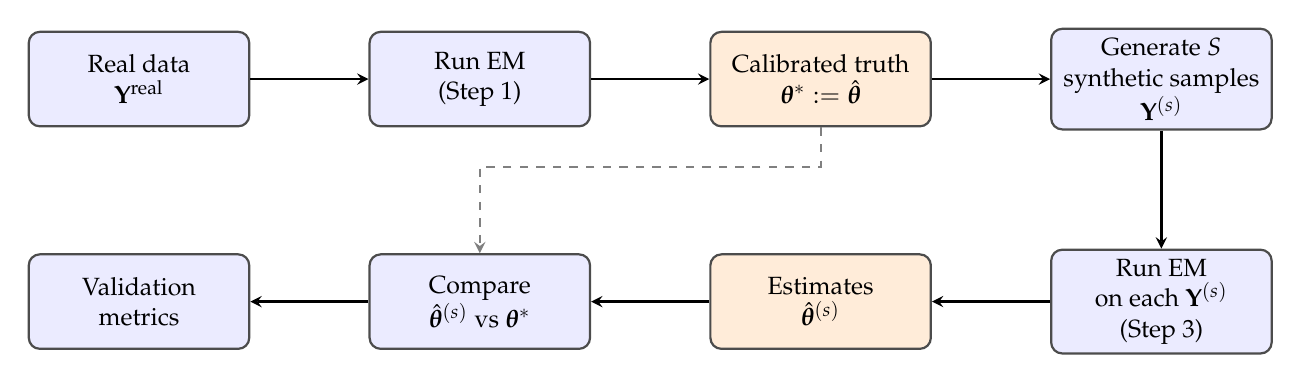
\begin{tikzpicture}[
    node distance=1.5cm,
    box/.style={
        rectangle, rounded corners,
        draw=black!70, thick,
        fill=blue!8,
        minimum width=2.8cm, minimum height=1.2cm,
        align=center, font=\small
    },
    truth/.style={
        rectangle, rounded corners,
        draw=black!70, thick,
        fill=orange!15,
        minimum width=2.8cm, minimum height=1.2cm,
        align=center, font=\small
    },
    arrow/.style={->, thick, >=stealth}
]

% Top row: from real data to synthetic samples
\node[box] (real) {Real data\\$\mY^{\mathrm{real}}$};
\node[box, right=of real] (em1) {Run EM\\(Step 1)};
\node[truth, right=of em1] (theta) {Calibrated truth\\$\boldsymbol{\theta}^* := \hat{\boldsymbol{\theta}}$};
\node[box, right=of theta] (gen) {Generate $S$\\synthetic samples\\$\mY^{(s)}$};

% Arrows top row
\draw[arrow] (real) -- (em1);
\draw[arrow] (em1) -- (theta);
\draw[arrow] (theta) -- (gen);

% Second row: re-estimation and comparison
\node[box, below=1.5cm of gen] (em2) {Run EM\\on each $\mY^{(s)}$\\(Step 3)};
\node[truth, left=of em2] (est) {Estimates\\$\hat{\boldsymbol{\theta}}^{(s)}$};
\node[box, left=of est] (compare) {Compare\\$\hat{\boldsymbol{\theta}}^{(s)}$ vs $\boldsymbol{\theta}^*$};
\node[box, left=of compare] (metrics) {Validation\\metrics};

% Arrows second row
\draw[arrow] (gen) -- (em2);
\draw[arrow] (em2) -- (est);
\draw[arrow] (est) -- (compare);
\draw[arrow] (compare) -- (metrics);

% Vertical arrow connecting theta to compare (ground truth feeds into comparison)
\draw[arrow, dashed, gray] (theta) |- ([yshift=-0.5cm]theta.south) -| (compare.north);

\end{tikzpicture}
\caption{The three-step Monte Carlo design. The real data
are used to calibrate the true parameter vector $\boldsymbol{\theta}^*$
(orange boxes mark ground truth). Synthetic samples are then
generated from this $\boldsymbol{\theta}^*$ and re-estimated; the
resulting estimates $\hat{\boldsymbol{\theta}}^{(s)}$ are compared against
the calibrated truth to assess parameter recovery.}
\label{fig:mc-three-step}
\end{figure}

\subsection{Simulating Realistic Empirical Conditions}
\label{subsec:mc-simulation}

A Monte Carlo experiment is only as informative as its similarity to
the empirical setting it aims to validate. If the synthetic data
generated in Step 2 are a stylised idealisation of the real panel —
balanced, single-frequency, free of outliers — then the algorithm's
performance on this synthetic data will overstate its performance on
the real macroeconomic series, where none of these idealisations
hold. The credibility of the validation therefore depends on
reproducing, in the simulated data, the empirical features that make
the real estimation problem hard.

This subsection describes how each such feature is reproduced
operationally. Six aspects of the empirical setting are considered;
we briefly introduce each of them here, before developing them in
dedicated subsections.

\paragraph{(i) Student-$t$ scale-mixture innovations.}
The data-generating process at the heart of the experiment is the
Student-$t$ DFM developed in this thesis. The innovations to the
factor process $u_t$ and to the observation equation
$\varepsilon_t$ are generated via the scale-mixture representation:
Gaussian shocks whose covariance is scaled by an independent Gamma
weight, with degrees of freedom equal to the calibrated
$\nu_u^*, \nu_\varepsilon^*$. This construction produces the heavy
tails that the Gaussian benchmark cannot reproduce, and it stores
the latent weight paths $\{w_t^{u,(s)}, w_t^{\varepsilon, (s)}\}$
as ground truth for the validation of the algorithm's
weight-recovery step.

\paragraph{(ii) Ragged-edge missingness.}
Real macroeconomic data are released with publication delays that
differ across series: at any sample date $T$, some series are
already available for the current period while others are still to
be released. The cross-section at the right edge of the panel is
therefore \emph{ragged}, with progressively sparser observations
as one approaches $T$. The Monte Carlo reproduces this pattern by
recording the missingness structure of the real data — encoded by
the selection matrices $\{\mathbf{W}_t^{\mathrm{real}}\}$ — and
imposing it on every synthetic sample before re-estimation. This
ensures that the synthetic estimation problem confronts the same
information structure as the empirical one, including the
asymmetric concentration of missing data at the most recent
periods.

\paragraph{(iii) Mixed-frequency calendar.}
A fraction of the series in the panel are observed at quarterly
rather than monthly frequency — including the target variable GDP.
The model handles this through the Mariano--Murasawa augmentation
of the state vector and a corresponding loading pattern. To
reproduce the same difficulty in the synthetic setting, we generate
the data at monthly frequency for all series, including those that
are observed only quarterly in the real panel; we then mask all
non-quarter-end months for the quarterly series, so that the
re-estimation step sees the same pattern of quarterly observations
that the real data exhibits. The latent monthly values of the
quarterly series remain stored as ground truth, allowing us to
evaluate whether the algorithm correctly interpolates them.

\paragraph{(iv) Block-diagonal economic identification.}
The DFM developed in this thesis imposes a block-diagonal structure
on the loading matrix: real-activity series load only on the real
factor, financial series only on the financial factor, and so on.
This identification restriction distinguishes our framework from
the unrestricted DFM of Doz, Giannone, and Reichlin (2012) and
gives the factors an economic interpretation. The same restriction
is preserved both in the data generation and in the re-estimation
of the synthetic samples, so that the Monte Carlo evaluates the
algorithm \emph{within} the identified model, not in an
unrestricted setting. This in turn allows us to test whether the
block identification is itself correctly recovered — that is,
whether the estimated real factor tracks the true real factor
rather than some linear combination involving the other blocks.

\paragraph{(v) Contamination by extreme observations.}
The Student-$t$ framework is motivated by the empirical observation
that macroeconomic series occasionally exhibit extreme realisations
— crisis episodes, pandemics, abrupt policy interventions — that
the Gaussian model would dismiss as overwhelmingly unlikely. To
quantify the robustness margin of the proposed estimator under this
empirical reality, a third experiment generates data from a
Gaussian DGP contaminated by a small fraction $\pi$ of outlier
periods drawn from a heavy-tailed distribution. The contamination
intensity $\pi$ is varied across the grid
$\{0.01,\, 0.05,\, 0.10\}$, tracing a continuous path from
near-Gaussian conditions to substantially contaminated ones. This
experiment is the most economically meaningful of the three, as it
reproduces the realistic case in which the baseline data are
well-behaved but a small minority of periods is governed by a
different mechanism that produces extreme observations.

\paragraph{(vi) Vintages and the real-time data flow.}
The news framework developed in the previous section operates on
\emph{vintages} — snapshots of the panel at different calendar
dates, reflecting the sequential arrival of new releases. To
validate the news framework in the Monte Carlo, the simulation
must reproduce the vintage structure of the real data: the release
calendar of each series, the sequence of vintages it generates,
and the corresponding pattern of forecast revisions. Although the
systematic empirical analysis of the news framework is deferred to
future work, the vintage-generation infrastructure is built into
the simulation pipeline described below, so that the validation
exercise can be extended to the news framework without further
infrastructure development.

\paragraph{Why all six matter.}
The six features cannot be sacrificed individually without
compromising the credibility of the validation. Generating data
without scale-mixture innovations would amount to using a Gaussian
DGP in all experiments, which would prevent any test of the
Student-$t$ machinery (a problem we address by varying the DGP
across the three experiments below). Synthetic data without
ragged-edge would make the estimation problem easier than the
empirical one. Synthetic data without mixed-frequency would not
test the Mariano--Murasawa machinery that is central to the model.
Synthetic data without block identification would not test the
economic interpretation of the factors. A Monte Carlo without
contamination experiments would not reveal the robustness margin
that motivates the heavy-tailed extension in the first place.
Synthetic data without vintages would not test the news framework.
Taken together, the six features turn the calibrated Monte Carlo
from a stylised exercise into a genuine reproduction of the
empirical estimation problem. The remaining subsections describe
how each feature is implemented in practice.

\subsubsection*{(i) The Student-$t$ Scale-Mixture}
\label{subsubsec:sim-scale-mixture}

\paragraph{Where we are in the design.}
Recall the structure of the Monte Carlo design: Step 1 estimated
the Student-$t$ DFM on the real data, producing the calibrated
parameter vector
\[
\btheta^* \;=\; (\mL^*,\, \mA^*,\, \mQ^*,\, \mR^*,\, \nu_u^*,\, \nu_\varepsilon^*),
\]
which is now treated as the ground truth of the Monte Carlo. Step 2
— which is what this subsection describes — generates the $S$
synthetic samples $\{\mY^{(s)}\}_{s=1}^{S}$ that the EM in Step 3
will see. The current question is therefore: \emph{given the
calibrated parameters $\btheta^*$, how do we generate a synthetic
sample from the Student-$t$ DFM?}

\paragraph{Why a scale-mixture, and not direct sampling.}
The Student-$t$ distribution does not have a standard primitive
random-number generator in most numerical libraries, and even where
one exists, sampling directly from a multivariate Student-$t$ would
not produce the latent objects (the weights) that the algorithm
recovers in the E-step. We therefore exploit the
\emph{scale-mixture representation} of the multivariate Student-$t$:
\[
y \sim t_{\nu}(\mathbf{0}, \boldsymbol{\Sigma})
\;\;\Longleftrightarrow\;\;
y \,\big|\, w \sim \mathcal{N}\!\big(\mathbf{0}, \boldsymbol{\Sigma}/w\big),
\quad
w \sim \mathrm{Gamma}\!\big(\nu/2,\, \nu/2\big).
\]
This identity says that a Student-$t$ draw is equivalent to a
two-step procedure: first draw a Gamma weight $w$, then draw a
Gaussian conditional on $w$ with covariance scaled by $1/w$.
Marginalising over $w$, the resulting $y$ has exactly a
Student-$t$ distribution with $\nu$ degrees of freedom.

This representation is both \emph{numerically efficient} — Gaussian
draws and Gamma draws are both standard primitives — and
\emph{methodologically transparent}: it makes the latent weights
$w_t^u, w_t^\varepsilon$ explicit at every period, so that we can
store them as ground truth against which the EM-estimated weights
$\hat{w}_t^u, \hat{w}_t^\varepsilon$ will later be compared.

\paragraph{A clarification on the weights.}
A subtle but important point: the weights drawn in this subsection
are entirely \emph{new}, independent draws from the marginal Gamma
distribution. They are not the smoothed weights
$\hat{w}_t^{u, \mathrm{real}}, \hat{w}_t^{\varepsilon, \mathrm{real}}$
that the EM in Step 1 produced on the real data — those were
specific to the real realisation and would have no role here. The
key insight is that in the scale-mixture representation, the
weights are not parameters of the model; they are \emph{latent
random variables} whose distribution is fully determined by the
parameter $\nu^*$. Once $\nu_u^*$ and $\nu_\varepsilon^*$ are
known — as they are, from the calibration step — generating new
weights for the synthetic samples is a direct probabilistic
operation: draw from $\mathrm{Gamma}(\nu^*/2, \nu^*/2)$. No
estimation or smoothing is involved.

This is the central conceptual point of the Monte Carlo
construction: each synthetic replication $s$ is a fresh
realisation of the data-generating process, with its own
independent latent weight paths and its own independent factor
and idiosyncratic shocks. The EM that re-estimates each
synthetic sample in Step 3 will, in turn, recover smoothed weight
paths $\hat{w}_t^{u, (s)}, \hat{w}_t^{\varepsilon, (s)}$ specific
to that replication, and these can be compared against the
ground-truth $w_t^{u, (s)}, w_t^{\varepsilon, (s)}$ drawn here to
assess the accuracy of the weight-recovery step.

\paragraph{The three-step procedure for each replication.}
With this setup in mind, the procedure for each replication $s$
proceeds in three sub-steps, described in order below: draw the
two latent weight paths (Step i.a), draw the factor path
conditional on the factor weights (Step i.b), and draw the
observations conditional on both factors and idiosyncratic weights
(Step i.c).

\paragraph{Step (i.a) — Draw the latent weight paths.}
We begin by drawing two independent weight paths for the entire
synthetic sample $t = 1, \ldots, T^*$, one for the factor process
and one for the observation process:
\begin{align}
w_t^{u, (s)} \;&\sim\; \mathrm{Gamma}\!\big(\nu_u^*/2,\, \nu_u^*/2\big), \\[2pt]
w_t^{\varepsilon, (s)} \;&\sim\; \mathrm{Gamma}\!\big(\nu_\varepsilon^*/2,\, \nu_\varepsilon^*/2\big),
\end{align}
with the draws independent across time and across the two
processes. The Gamma distribution is parametrised with shape and
rate both equal to $\nu^*/2$, a convention that gives the weights
two convenient properties: their unconditional mean is one
($\mathbb{E}[w_t] = 1$) and their variance is $2/\nu^*$.

The role of $\nu^*$ is therefore entirely captured by this single
quantity: smaller $\nu^*$ produces larger variance in the weights,
which in turn produces a wider spread of the conditional
covariances of the Gaussian shocks across $t$, which finally
translates into heavier tails of the marginal Student-$t$
distribution. The calibrated values $\nu_u^*, \nu_\varepsilon^*$
that we extracted from the real data therefore directly determine
the empirical realism of the heavy tails in the synthetic samples.
A typical macroeconomic calibration yields
$\nu^* \in [8, 15]$, which produces weights tightly distributed
around one for most periods and substantially below one for a
small fraction of outlier-prone periods.

\paragraph{Step (i.b) — Draw the factor path conditional on weights.}
With the factor weights $\{w_t^{u, (s)}\}$ drawn, the factor
innovations $u_t^{(s)}$ are conditionally Gaussian with time-varying
covariance:
\[
u_t^{(s)} \,\big|\, w_t^{u, (s)} \;\sim\; \mathcal{N}\!\Big(\mathbf{0},\, \mQ^* / w_t^{u, (s)}\Big),
\qquad t = 1, \ldots, T^*.
\]
A period with $w_t^{u, (s)} \approx 1$ produces a near-typical
innovation; a period with $w_t^{u, (s)}$ substantially below one
produces an innovation drawn from a distribution with inflated
covariance — exactly the mechanism through which Student-$t$
heavy tails are operationalised.

The factor path is then constructed recursively from the state
equation, after initialising at the stationary distribution of the
VAR(1):
\begin{align}
f_0^{(s)} \;&\sim\; \mathcal{N}\!\big(\mathbf{0},\, \boldsymbol{\Sigma}_0\big), \qquad
\mathrm{vec}(\boldsymbol{\Sigma}_0) \;=\; \big(I_{r^2} - \mA^* \otimes \mA^*\big)^{-1} \mathrm{vec}(\mQ^*), \\[2pt]
f_t^{(s)} \;&=\; \mA^* f_{t-1}^{(s)} \;+\; u_t^{(s)}, \qquad t = 1, \ldots, T^*.
\end{align}
The choice to initialise at the stationary distribution rather
than at the origin is deliberate: it avoids the transient effect
that would arise if $f_0 = \mathbf{0}$, in which the first
several periods of the simulated path would be artificially close
to zero while the dynamics propagate the recent shocks. By drawing
$f_0$ directly from the stationary distribution, we ensure that
the entire simulated path is statistically homogeneous across
time.

\paragraph{Step (i.c) — Draw the observations conditional on factors and weights.}
With the factor path $\{f_t^{(s)}\}$ constructed and the
idiosyncratic weights $\{w_t^{\varepsilon, (s)}\}$ already drawn in
Step (i.a), the idiosyncratic shocks $\varepsilon_t^{(s)}$ are
conditionally Gaussian with time-varying diagonal covariance:
\[
\varepsilon_t^{(s)} \,\big|\, w_t^{\varepsilon, (s)} \;\sim\; \mathcal{N}\!\Big(\mathbf{0},\, \mR^* / w_t^{\varepsilon, (s)}\Big),
\]
and the synthetic observations are assembled from the observation
equation:
\[
y_t^{(s)} \;=\; \mL^* f_t^{(s)} \;+\; \varepsilon_t^{(s)}, \qquad t = 1, \ldots, T^*.
\]
The product $\mL^* f_t^{(s)}$ is the common-factor component of
$y_t^{(s)}$, capturing the cross-sectional comovement driven by
the latent factors; $\varepsilon_t^{(s)}$ is the series-specific
idiosyncratic component, with its own heavy-tailed weight process
operating independently from the factor weights.

\paragraph{What is stored for ground truth.}
At the end of the three steps above, the simulation produces — for
each replication $s$ — two distinct categories of objects:
\begin{itemize}[leftmargin=1.5em, itemsep=3pt]
    \item \emph{Observable panel}: the synthetic observations
          $\{y_t^{(s)}\}_{t=1}^{T^*}$. This is what the EM
          algorithm in Step 3 of the Monte Carlo design has access
          to. The ragged-edge missingness pattern and the
          mixed-frequency calendar are then imposed on this panel
          as described in the subsections that follow, before the
          re-estimation step.
    \item \emph{Latent ground truth}: the factor path
          $\{f_t^{(s)}\}$, the weight paths
          $\{w_t^{u, (s)}, w_t^{\varepsilon, (s)}\}$, and the
          idiosyncratic shocks $\{\varepsilon_t^{(s)}\}$. These
          are the objects that the EM algorithm \emph{would} need
          to know but does not — and that the Monte Carlo uses to
          assess how well the EM-recovered smoothed counterparts
          $\hat{f}_t^{(s)}, \hat{w}_t^{u, (s)},
          \hat{w}_t^{\varepsilon, (s)}$ approximate them.
\end{itemize}
The strict separation between observable panel and latent ground
truth is what makes the Monte Carlo a meaningful validation
exercise: the algorithm operates on what it would see in the real
world, while the validation has access to what really drove the
data.

\subsubsection*{(ii) Ragged-Edge Missingness}
\label{subsubsec:sim-ragged-edge}

\paragraph{The empirical feature to reproduce.}
Real macroeconomic data are released with publication delays that
vary substantially across series: GDP is published roughly one
month after the end of the reference quarter, employment data are
released with a one-month delay, industrial production with about
six weeks, while financial conditions indices and stock-market
indicators are available essentially in real time. The practical
consequence is that, at any given sample date $T$, the most recent
months of the panel exhibit a characteristic \emph{ragged} pattern:
the last column of the data matrix is sparse, populated only by
the few series with no delay; the second-to-last column is
denser; and so on, until past months in which all series have
eventually been released.

This pattern is not a curiosity — it is the defining empirical
challenge of \emph{nowcasting}, the activity of producing
real-time estimates of variables (such as GDP) that have not yet
been officially released. The mixed-frequency framework, the
Kalman filter and smoother with selection matrices $\mathbf{W}_t$,
and the news framework developed earlier in this thesis are
specifically designed to handle this ragged structure. The Monte
Carlo must therefore confront the same difficulty: a synthetic
panel that is fully balanced at all $t$ would not test the
nowcasting machinery at all.

\paragraph{Why the DGP alone does not generate ragged-edge.}
A clarification is in order. The Student-$t$ DFM described in
Step (i) generates, for each $t = 1, \ldots, T^*$, a complete
cross-section of $M$ observations $y_t^{(s)}$. There is no
mechanism within the model itself that would make any entry of
$y_t^{(s)}$ missing: missingness in the real data is a property of
the \emph{release calendar}, not of the data-generating process.
We therefore impose ragged-edge missingness on the synthetic data
\emph{ex post}, after the balanced panel has been generated, by
applying the same selection matrices that the EM uses on the real
data.

\paragraph{Imposing the real-data pattern.}
During the calibration of Step 1, we record the selection matrix
$\mathbf{W}_t^{\mathrm{real}}$ for every $t = 1, \ldots, T_{\mathrm{real}}$
in the real panel. Each $\mathbf{W}_t^{\mathrm{real}}$ is a
diagonal $M \times M$ matrix whose $(i, i)$ entry equals $1$ if
series $i$ has been observed at time $t$ in the real data, and
$0$ otherwise. The full sequence
$\{\mathbf{W}_t^{\mathrm{real}}\}_{t = 1}^{T_{\mathrm{real}}}$
encodes the entire publication-delay structure of the empirical
sample.

For each synthetic sample $\mY^{(s)}$ of length
$T^* = T_{\mathrm{real}}$, we apply this same selection matrix
sequence to construct the version of the synthetic data that the
EM algorithm will actually see:
\[
\mY^{(s), \mathrm{ragged}}_t \;=\; \mathbf{W}_t^{\mathrm{real}}\, y_t^{(s)},
\qquad t = 1, \ldots, T_{\mathrm{real}}.
\]
The operation is deterministic: it sets to zero (or, equivalently,
to ``missing'') exactly those entries of $y_t^{(s)}$ that would
have been missing in the corresponding period of the real data.
Two properties of this construction are worth emphasising:
\begin{itemize}[leftmargin=1.5em, itemsep=3pt]
    \item The fully observed synthetic vector $y_t^{(s)}$ remains
          \emph{stored as ground truth} alongside the ragged-edge
          version. The masked entries are not lost — they are
          simply hidden from the EM. This allows us to evaluate,
          ex post, how well the algorithm imputes the missing
          entries using only the observed ones.
    \item The EM in Step 3 sees only $\mY^{(s), \mathrm{ragged}}$,
          never $y_t^{(s)}$. Its task is exactly the empirical
          task: recover the underlying parameters and the latent
          factor path from a panel whose right edge is sparse,
          using the selection matrices to handle the missing
          entries.
\end{itemize}
The resulting synthetic estimation problem is therefore
informationally equivalent to the empirical one, by construction.

\paragraph{Synthetic samples of different length.}
A subtle issue arises when the Monte Carlo varies the sample size
$T^* \neq T_{\mathrm{real}}$, as required by the finite-sample
analysis described earlier. The recorded missingness pattern
$\{\mathbf{W}_t^{\mathrm{real}}\}$ has length exactly
$T_{\mathrm{real}}$, so it cannot be applied verbatim to a
synthetic sample of different length.

We adopt a simple convention: the ragged-edge structure is
concentrated at the right edge of the panel, and its depth in
real data is typically only a few months (the so-called
\emph{ragged region}, of length $T_{\mathrm{real, ragged}}$,
which is generally between $3$ and $6$ months depending on the
publication delays of the series included in the panel). For a
synthetic sample of length $T^*$, we apply the real ragged-edge
pattern to the last $T_{\mathrm{real, ragged}}$ periods of the
sample (mapping the relative position of each release to its
real-data counterpart), and treat the remaining $T^* - T_{\mathrm{real, ragged}}$
periods as a fully observed balanced panel.

This convention preserves the qualitative difficulty of
ragged-edge estimation — the EM still faces a sparse right edge
in each replication — while accommodating synthetic samples of
arbitrary length. It is consistent with the assumption that the
publication-delay structure is a recent-period phenomenon, not a
sample-wide one: in historical data, sufficiently old periods are
fully observed.

\subsubsection*{(iii) Mixed-Frequency Observations}
\label{subsubsec:sim-mixed-frequency}

\paragraph{The empirical feature to reproduce.}
A fraction of the series in the panel — and in particular the
target variable GDP — are observed at \emph{quarterly} rather than
monthly frequency. This is not a feature of the data-generating
process: at the underlying level, factors and shocks evolve at
monthly frequency, and the macroeconomic activity they describe
is itself a continuous flow. What is quarterly is the
\emph{measurement}: the statistical agency aggregates three months
of activity into a single quarterly observation, releases the
result roughly one month after the end of the quarter, and that
single number is all that the analyst sees.

Throughout this thesis we have handled this mismatch through the
Mariano--Murasawa augmented state-space representation, in which
each quarterly series is treated as a monthly series observed only
at quarter-end months, loaded on the composite regressor
\[
\phi^k_t \;=\; \tfrac{1}{3} f_t \;+\; \tfrac{2}{3} f_{t-1} \;+\; f_{t-2} \;+\; \tfrac{2}{3} f_{t-3} \;+\; \tfrac{1}{3} f_{t-4}.
\]
The five lagged factors and the specific MM weights reflect the
log-difference structure of the quarter-on-quarter growth rate of
the underlying monthly process. The Monte Carlo must therefore
generate synthetic data that confront the EM with this same
mismatch: a panel in which some series are observed at every
month and others only at quarter-end months, with the
quarterly entries representing the MM-aggregated monthly path.

\paragraph{Why the DGP generates everything at monthly frequency.}
A clarification analogous to the one made for ragged-edge
missingness applies here. The Student-$t$ DFM specified in
Step (i) generates a complete monthly path $f_t^{(s)}$ for the
latent factors, and from this path a complete monthly observation
$y_{i,t}^{(s)} = \boldsymbol{\Lambda}_{i \cdot}^*\, f_t^{(s)} + \varepsilon_{i,t}^{(s)}$
is produced for \emph{every} series in the panel, regardless of
whether that series is observed monthly or quarterly in the real
data. There is no separate ``quarterly'' DGP: the model assumes
that the underlying economic activity of every series exists at
monthly frequency, and that quarterly observability is purely a
measurement convention imposed by the release calendar.

The synthetic monthly path of a quarterly series is therefore the
\emph{latent} monthly counterpart of the quarterly observations
that the real data would release. As with ragged-edge missingness,
the calendar-induced unobservability is imposed on this full
monthly path in a separate, deterministic step.

\paragraph{Imposing the quarterly aggregation.}
Let $j$ denote a quarterly series — i.e.\ a series that in the real
data is only observed at quarter-end months. Step (i) has generated
a full \emph{latent monthly path} for this series:
\[
y_{j, t}^{(s)} \;=\; \boldsymbol{\Lambda}^{Q, *}_{j \cdot}\, \tilde{f}_t^{(s)} \;+\; \varepsilon_{j, t}^{(s)},
\qquad t = 1, \ldots, T^*,
\]
where $\boldsymbol{\Lambda}^{Q, *}_{j \cdot}$ is the Mariano--Murasawa
row of the loading matrix for series $j$ — with the five weighted
entries
$[\tfrac{1}{3}\boldsymbol{\Lambda}^Q_{j \cdot},\, \tfrac{2}{3}\boldsymbol{\Lambda}^Q_{j \cdot},\, \boldsymbol{\Lambda}^Q_{j \cdot},\, \tfrac{2}{3}\boldsymbol{\Lambda}^Q_{j \cdot},\, \tfrac{1}{3}\boldsymbol{\Lambda}^Q_{j \cdot}]$
Note that $y_{j, t}^{(s)}$ is a \emph{monthly} value, even though
the series $j$ is intrinsically quarterly: it is the value that the
series would have if it were observed monthly.

The quarterly aggregation that the real data imposes is then
applied by masking this latent monthly path at all months other
than quarter-end:
\[
\tilde{y}_{j, t}^{(s)} \;=\;
\begin{cases}
y_{j, t}^{(s)} & \text{if $t$ is a quarter-end month,} \\
\text{missing} & \text{otherwise.}
\end{cases}
\]
The EM in Step 3 sees only the masked panel $\tilde{y}_{j, t}^{(s)}$:
one observation every three months at quarter-end calendar dates,
exactly as in the real data. The latent monthly values at
non-quarter-end months are hidden from the algorithm but stored
alongside the masked panel as ground truth.

\paragraph{What this enables.}
This design provides two distinct ground-truth objects against
which the EM in Step 3 can be evaluated.

First, the algorithm produces smoothed estimates of the latent
monthly values $\hat{y}_{j, t}^{(s)}$ at the non-quarter-end
months through the Kalman smoother applied to the augmented
state-space. These estimates are the model's reconstruction of
the latent monthly path of the quarterly series $j$ — that is,
the very task that the Mariano--Murasawa framework was designed
to perform. The Monte Carlo allows us to compare them directly
against the true generated values $y_{j, t}^{(s)}$, quantifying
how well the algorithm interpolates between consecutive
quarter-end observations.

Second, the algorithm produces estimates of the quarterly loading
matrix $\hat{\boldsymbol{\Lambda}}^Q$, including the specific
Mariano--Murasawa pattern of five weighted entries
$[\tfrac{1}{3}\boldsymbol{\Lambda}^Q,\, \tfrac{2}{3}\boldsymbol{\Lambda}^Q,\, \boldsymbol{\Lambda}^Q,\, \tfrac{2}{3}\boldsymbol{\Lambda}^Q,\, \tfrac{1}{3}\boldsymbol{\Lambda}^Q]$.
These estimates can be compared against the true
$\boldsymbol{\Lambda}^{Q, *}$ that generated the synthetic data,
testing whether the EM correctly identifies the magnitude of the
loading and the specific MM structure imposed by the augmented
representation.

Together, these two validation outputs test the mixed-frequency
machinery of the model from two complementary angles: the recovery
of the latent monthly path (a smoother quality test) and the
recovery of the parameter that maps factors to quarterly series
(a maximum-likelihood quality test).

\subsubsection*{(iv) Block-Diagonal Economic Identification}
\label{subsubsec:sim-block-structure}

\paragraph{The empirical feature to reproduce.}
The DFM developed in this thesis imposes a \emph{block-diagonal}
structure on the loading matrix: real-activity series load only on
the real factor, financial series only on the financial factor,
and the residual ``other'' series load only on the third block.
This is an \emph{economic identification restriction} that
distinguishes our setting from the unrestricted DFM of Doz,
Giannone, and Reichlin (2012), where the factors are extracted
purely statistically and have no inherent economic interpretation.

The motivation for the restriction is interpretability: by forcing
each factor to capture variation in a specific economic domain,
we obtain factors that can be unambiguously labelled as
``real activity'', ``financial conditions'', and ``other''. This
labelling is essential for the Growth-at-Risk analysis of the
second stage, where the financial-conditions factor plays a
distinct role in shaping the lower tail of the GDP distribution.
A factor model that mixes real and financial influences across
the same factor would not support this kind of structural
interpretation.

The Monte Carlo must therefore preserve the block-diagonal
structure throughout: in the data generation, in the re-estimation,
and in the comparison between estimates and ground truth.

\paragraph{Why the structure must be imposed everywhere.}
Block-diagonality is not a feature of the data that emerges
spontaneously from the DGP — it is a \emph{constraint} on the
parameter space. Without it, the EM has no reason to allocate
each series to a specific factor: the rotational indeterminacy
discussed earlier in the thesis means that an unrestricted DFM
can always rotate the factors to redistribute the loading mass
across them, yielding statistically equivalent but economically
meaningless representations. Imposing the block structure removes
this freedom and pins down a specific economic identification.

For the Monte Carlo to evaluate the proposed estimator
meaningfully, the same restriction must be applied at every step:
\begin{itemize}[leftmargin=1.5em, itemsep=3pt]
    \item In the \emph{calibration} of Step 1, the EM applied to
          $\mY^{\mathrm{real}}$ imposes the block-diagonal
          structure during estimation, producing
          $\mL^*$ with the appropriate zero entries off the
          diagonal blocks.
    \item In the \emph{data generation} of Step 2, the same
          $\mL^*$ is used verbatim: there are no off-block
          loadings, by construction. The synthetic factor paths
          $\{f^{R, (s)}, f^{F, (s)}, f^{X, (s)}\}$ each drive only
          their respective block of series.
    \item In the \emph{re-estimation} of Step 3, the EM applied to
          each synthetic sample imposes the same block-diagonal
          constraint on its loading estimates
          $\hat{\mL}^{(s)}$. The algorithm therefore operates
          within the same identified model that we want to
          validate.
\end{itemize}
Without this consistency, the Monte Carlo would be testing two
different models — and any disagreement between estimates and
truth could equally well be attributed to the mismatch in
identifying restrictions rather than to genuine estimation error.

\paragraph{What this lets us test.}
With the block-diagonal structure preserved across all three
steps, the Monte Carlo enables two distinct validation tests
specific to this identification.

The first test concerns the \emph{within-block loading magnitudes}.
For each block $b \in \{R, F, X\}$, the EM produces estimates
$\hat{\mL}^{b, (s)}$ of the rows of the loading matrix
corresponding to series in that block. These can be compared
against the true $\mL^{b, *}$ via the bias, variance, and RMSE
metrics introduced later. A successful recovery indicates that the
EM correctly identifies how strongly each series in a given block
loads on its block-specific factor.

The second test concerns the \emph{recovery of the block-specific
factors themselves}. The smoothed factor estimates
$\hat{f}^{R, (s)}, \hat{f}^{F, (s)}, \hat{f}^{X, (s)}$ produced by
the EM can be compared against the true factor paths
$f^{R, (s)}, f^{F, (s)}, f^{X, (s)}$ via per-block correlations
and trajectory errors. The key question this test answers is
whether each estimated block factor tracks the corresponding true
factor specifically — for example, whether $\hat{f}^R$ correlates
with $f^{R, *}$ but \emph{not} with $f^{F, *}$. A high
within-block correlation combined with a near-zero cross-block
correlation
$\mathrm{Corr}(\hat{f}^R, f^{F, *})$ provides strong evidence
that the block-diagonal identification is empirically respected
by the algorithm.

These two tests together address whether the economic
identification of the model is statistically robust: the loadings
are correctly assigned within blocks, and the factors are
correctly assigned across blocks.

\subsubsection*{(v) Contamination by Extreme Observations}
\label{subsubsec:sim-contamination}

\paragraph{The empirical feature to reproduce.}
The Student-$t$ framework developed in this thesis is motivated by
a specific empirical observation about macroeconomic data:
\emph{most of the time, the data behave well} — series move
together, shocks are moderate in magnitude, and the standard
Gaussian DFM provides a reasonable approximation. But a small
minority of periods are governed by entirely different mechanisms:
crisis episodes (the global financial crisis of 2008--2009),
abrupt policy interventions, pandemics (the Covid-19 shock of
2020), or geopolitical events that produce extreme realisations
the Gaussian model would treat as overwhelmingly unlikely.

These extreme periods are not just statistical curiosities: they
are precisely the periods where a Growth-at-Risk analysis is most
needed — when the lower tail of the GDP distribution is at its
most informative, and when a forecasting model must remain
reliable. A Gaussian DFM, applied to such data, absorbs the
extreme realisations into its covariance estimates, inflating
them and distorting the factor recovery. The Student-$t$ extension
is designed precisely to recognise these periods as outliers,
down-weight their contribution, and preserve the integrity of the
estimates from the bulk of the sample.

\paragraph{What this experiment is designed to quantify.}
Experiments A and B describe two limiting cases: a fully
Student-$t$ DGP (Experiment A, where the heavy-tailed extension
should outperform the Gaussian benchmark) and a fully Gaussian DGP
(Experiment B, where the two estimators should agree by the
nesting property). Real macroeconomic data lie between these two
extremes: predominantly Gaussian, with sporadic outlier-prone
periods. Experiment C — the contamination experiment described in
this subsubsection — fills this intermediate region by varying
the fraction $\pi$ of contaminated periods across a grid, tracing
a continuous path from the Gaussian endpoint to substantially
contaminated regimes.

The experiment provides a quantitative measure of the
\emph{robustness margin} of the Student-$t$ extension: how much
worse the Gaussian benchmark performs as $\pi$ grows, and how
stably the Student-$t$ estimator maintains its accuracy. This is
the most economically meaningful of the three experiments,
because it most closely reproduces the empirical reality of the
data we actually want to analyse.

\paragraph{The contamination mechanism.}
Let $\pi \in \{0,\, 0.01,\, 0.05,\, 0.10\}$ denote the
\emph{contamination intensity} --- the fraction of time periods
governed by the outlier mechanism. The three positive values
correspond roughly to one in a hundred, one in twenty, and one in
ten time periods being affected; the value $\pi = 0$ is included
deliberately as an anchor, since at $\pi = 0$ the data-generating
process is purely Gaussian and the experiment reduces \emph{exactly}
to Experiment B (this provides an internal consistency check: the
two estimators must coincide there by the nesting property). 

For each $t$ in the synthetic sample, we draw an independent Bernoulli indicator
\[
z_t \;\sim\; \mathrm{Bernoulli}(\pi),
\]
which determines whether period $t$ is contaminated ($z_t = 1$) or
not ($z_t = 0$). The indicator is indexed by \emph{time}, not by
the series--time pair: when a period is flagged as contaminated,
the outlier mechanism applies to the \emph{entire} idiosyncratic
vector at that period, affecting all $M$ series simultaneously.
This reflects the empirical observation that extreme periods ---
a crisis month, a policy shock --- are system-wide events felt
across the whole cross-section, not isolated glitches in a single
series. Conditional on $z_t = 1$, the idiosyncratic shock at $t$
is \emph{replaced} (not augmented) by a draw from a heavy-tailed
Student-$t$ distribution with low degrees of freedom and inflated
scale:
\[
\varepsilon_t^{(s)} \,\big|\, z_t = 1 \;\sim\;
t_{\nu_{\mathrm{contam}}}\!\big(\mathbf{0},\, \kappa^2 \mR^*\big),
\]
with $\nu_{\mathrm{contam}} = 3$ --- low enough to produce
visible, genuinely heavy-tailed outlier realisations --- and
$\kappa = 5$, so that the conditional idiosyncratic variance is
$\kappa^2 = 25$ times the Gaussian baseline (roughly an order of
magnitude larger, making the contamination clearly distinguishable
from ordinary fluctuations). The substitutive mechanism --- the
contaminated shock replaces the Gaussian one rather than adding to
it --- ensures that $\pi = 0$ recovers the Gaussian baseline
exactly, period by period. For $t$ with $z_t = 0$, the standard
Gaussian shock applies. In implementation, the Student-$t$ draw is
generated through the same scale-mixture representation used
throughout this thesis: a single mixing weight
$w_t^{\mathrm{contam}} \sim \mathrm{Gamma}(\nu_{\mathrm{contam}}/2,
\nu_{\mathrm{contam}}/2)$, shared across the $M$ series of the
contaminated period, scales the inflated covariance
$\kappa^2 \mR^*$.

The factor innovations $u_t^{(s)}$ are not contaminated in this
experiment: only the idiosyncratic component is affected. This is
a deliberate choice that mirrors the empirical regularity that
extreme periods typically manifest as deviations \emph{from} the
underlying factor structure rather than as movements of the
factor itself — a stock-market crash, for instance, is felt as a
spike in the residual of financial series rather than as a shift
in the latent financial factor. (The case in which the factor is
also contaminated is a natural extension that we do not pursue
here.)

\paragraph{What this experiment isolates.}
The contamination mechanism produces a data-generating process
that is \emph{predominantly Gaussian} but with periodic excursions
into heavy-tailed territory. Three concrete predictions follow
from the comparative structure of the two estimators:
\begin{itemize}[leftmargin=1.5em, itemsep=3pt]
    \item As $\pi$ grows, the Gaussian EM should exhibit
          \emph{increasing bias and variance} in
          $\hat{\mL}, \hat{\mathbf{Q}}, \hat{\mR}$. The mechanism
          is direct: the Gaussian model has no way to distinguish
          contaminated from clean periods, so the extreme
          observations enter the covariance estimates as if they
          were typical realisations, inflating them and distorting
          the factor recovery.
    \item The Student-$t$ EM should remain \emph{comparatively
          stable} as $\pi$ grows. Its estimated
          $\hat{\nu}_\varepsilon$ adjusts to reflect the empirical
          tail thickness, decreasing as $\pi$ increases, and the
          posterior weights $\hat{w}_t^\varepsilon$ concentrate
          the down-weighting on the periods that were in fact
          contaminated.
    \item The Student-$t$ EM should \emph{identify} the truly
          contaminated periods through its posterior weights
          $\hat{w}_t^\varepsilon$: the contaminated periods, having
          generated extreme residuals, should receive the smallest
          weights. The effectiveness of this identification is
          quantified by a detection metric defined precisely below.
\end{itemize}
At $\pi = 0$ the experiment reduces exactly to Experiment B
(Gaussian DGP, both estimators should agree). As $\pi$ grows the
DGP approaches a fully heavy-tailed regime, and the comparison
approaches Experiment A. Experiment C therefore traces a
continuous interpolation between the two endpoints, with the
fraction of contamination $\pi$ as the natural parameter.

\subsubsection*{(vi) Vintages and the Real-Time Data Flow}
\label{subsubsec:sim-vintages}

\paragraph{The empirical feature to reproduce.}
The news framework developed earlier in this thesis does not
operate on a single static panel: it operates on a \emph{sequence}
of panels, each corresponding to a different calendar date and
reflecting the cumulative information available up to that date.
Each such snapshot is a \emph{vintage}. As new data releases occur,
the vintage expands: industrial production for January is released
around mid-February; payrolls for January is released on the first
Friday of February; the advance estimate of GDP for the quarter
ending January is released about one month after the quarter ends.
Each release moves one or more entries of the data matrix from
``not yet available'' to ``available'', producing a new vintage
that is strictly richer than its predecessor.

This sequential arrival of information is the empirical reality of
real-time nowcasting, and the news framework was specifically
constructed to quantify how each new release updates the forecast
of the target variable. For the Monte Carlo to validate the news
framework, the synthetic data must reproduce the same vintage
structure: a release calendar that determines when each $(i, t)$
observation becomes available, and a corresponding sequence of
expanding panels.

\paragraph{Why the DGP alone does not generate vintages.}
The data-generating process described in Step (i) produces a full
synthetic panel $\{y_t^{(s)}\}_{t=1}^{T^*}$ in which all entries
are simultaneously available — there is no notion of ``release
date'' in the DGP. As with ragged-edge missingness and quarterly
masking, the vintage structure is not a feature of the underlying
model but a feature of the empirical \emph{release calendar},
which the Monte Carlo must impose ex post on the generated data.

\paragraph{Recording and applying the release calendar.}
The real data come with a documented release calendar: for each
series $i$ and each reference period $t$, we know the calendar
date $v_{i, t}$ at which the corresponding observation became
available in real time. We record this calendar during the
calibration of Step 1 and apply it verbatim to each synthetic
sample $\mY^{(s)}$.

The calendar defines, implicitly, a partition of time into a
sequence of distinct \emph{release dates}: between two consecutive
release dates the information set is unchanged, and at each
release date one or more new observations are added. Let
$v_1 < v_2 < \cdots < v_V$ denote the ordered sequence of distinct
release dates encountered in the synthetic sample. For each
vintage $v_k$, we construct the data panel that would have been
observable at that date:
\[
\mathbf{Y}^{(s), v_k} \;=\;
\big\{\, y_{i, t}^{(s)} \,:\, v_{i, t} \leq v_k \,\big\},
\]
with all not-yet-released entries treated as missing. By
construction, the sequence
\[
\mathbf{Y}^{(s), v_1} \;\subset\; \mathbf{Y}^{(s), v_2} \;\subset\; \cdots \;\subset\; \mathbf{Y}^{(s), v_V}
\]
forms a filtration that mirrors the real-time information flow:
each vintage extends its predecessor by exactly the observations
released between the two corresponding calendar dates.

\paragraph{Sample-size invariance of the release structure.}
A subtle point arises when the Monte Carlo varies the sample size
$T^* \neq T_{\mathrm{real}}$. The release calendar of the real
data is encoded not by specific calendar dates, but by
publication \emph{lags} that are intrinsic to each series: GDP is
released approximately one month after the end of the reference
quarter, industrial production with a six-week delay, payrolls
with a one-week delay, financial conditions essentially in real
time. Let $d_i$ denote the publication lag of series $i$
(in months); then the release date of the observation
$y_{i, t}^{(s)}$ in the synthetic sample is
\[
v_{i, t} \;=\; t \;+\; d_i.
\]
This formulation depends only on $t$ and on the series-specific
lag $d_i$, not on the total length of the sample. The vintage
sequence and the filtration construction described above therefore
apply identically to samples of any length $T^*$: the structure
of the release calendar is sample-size invariant. Only the lags
$\{d_i\}$ must be recorded during the calibration of Step 1, not
the specific calendar dates.

\paragraph{What this enables for the news framework.}
With the vintage sequence available for each synthetic replication,
the Monte Carlo can directly test the news framework developed in
the previous section. For each pair of consecutive vintages
$(v_k, v_{k+1})$ and each replication $s$, two distinct objects
can be computed and compared:
\begin{itemize}[leftmargin=1.5em, itemsep=3pt]
    \item The \emph{theoretical news weights}
          $\mathbf{B}_{k, t_k}^{(v_{k+1})}$, obtained from the
          analytical expressions derived earlier, evaluated at the
          estimated parameters and smoothed covariances of the
          model at vintage $v_k$;
    \item The \emph{realised forecast revisions}, obtained by
          re-running the EM on the two vintage panels
          $\mathbf{Y}^{(s), v_k}$ and $\mathbf{Y}^{(s), v_{k+1}}$
          and recording the change in the implied target forecast.
\end{itemize}
The product of the theoretical weight matrix with the realised
news vector,
$\mathbf{B}_{k, t_k}^{(v_{k+1})}\, \mathcal{I}_{v_{k+1}}$, should
equal the realised revision up to numerical precision. Agreement
between the two constitutes evidence that the news framework, as
implemented within the Student-$t$ DFM, is internally consistent
and quantitatively accurate.

The Monte Carlo can also assess two more nuanced properties of
the framework. First, the distribution of news weights across
vintages reveals how the model attributes forecast revisions to
specific releases — a diagnostic that can be compared against
prior economic intuition. Second, the empirical role of the
Student-$t$ outlier-aware mechanism (the modulation of the news
weights by the estimated weights $\hat{w}_t^\varepsilon$ in
high-stress periods) can be quantified by comparing the weights
produced by the Student-$t$ EM against those produced by the
Gaussian benchmark applied to the same synthetic panels.

\paragraph{A note on scope.}
The vintage-based validation described here is a natural
extension of the parameter-recovery Monte Carlo developed in the
rest of this section, and one that we plan to develop fully in
future work. In the present thesis, we focus on the parameter
recovery experiments (Experiments A, B, and C as described
above), and we report the vintage-based validation as a planned
extension rather than as a fully implemented result. The
infrastructure for generating vintage data — the release
calendar, the sequence of expanding panels, the framework for
comparing theoretical and realised revisions — is already built
into the simulation pipeline, so that the vintage-based
validation can be carried out without additional infrastructure
development. The systematic empirical analysis of news weights and
their associated forecast revisions is the natural complement to
the empirical application of the news framework on real data, and
the two will be developed together in subsequent work.

\subsubsection*{Summary of the Simulation Pipeline}
\label{subsubsec:sim-summary}

\paragraph{The six elements together.}
The six elements described in this subsection — Student-$t$
scale-mixture innovations, ragged-edge missingness, mixed-frequency
aggregation, block-diagonal economic identification, outlier
contamination, and the vintage structure of real-time releases —
together produce synthetic samples whose statistical features
mirror those of the real macroeconomic panel. Each element targets
a specific empirical challenge that the proposed estimator must
confront: heavy-tailed innovations, ragged data, quarterly target
variables, structured factor loadings, periodic outlier regimes,
and a sequentially expanding information set. Together, they turn
the calibrated Monte Carlo from a stylised exercise into a genuine
reproduction of the empirical estimation problem.

\paragraph{The order of operations.}
The order in which these elements are applied to construct each
synthetic sample $\mY^{(s)}$ deserves to be made explicit, because
it reflects the conceptual structure of the data-generating
mechanism. For each replication $s$, the operations proceed in
the following sequence:
\begin{enumerate}[leftmargin=1.5em, itemsep=4pt]
    \item \emph{Draw the latent weight paths}
          $\{w_t^{u, (s)}, w_t^{\varepsilon, (s)}\}_{t=1}^{T^*}$
          from independent Gamma distributions with parameters
          derived from $\nu_u^*$ and $\nu_\varepsilon^*$.
    \item \emph{Draw the latent factor path}
          $\{f_t^{(s)}\}_{t=1}^{T^*}$ recursively, conditional on
          the factor weights, starting from the stationary
          distribution of the VAR(1).
    \item \emph{Draw the latent idiosyncratic shocks}
          $\{\varepsilon_t^{(s)}\}_{t=1}^{T^*}$ conditional on the
          idiosyncratic weights, with the block-diagonal
          covariance structure preserved.
    \item \emph{Inject contamination (Experiment C only)}: for
          each $t$, draw a Bernoulli indicator $z_t$ and, if
          $z_t = 1$, replace the idiosyncratic shock with a draw
          from the heavy-tailed contamination distribution.
    \item \emph{Compose the balanced observations}
          $y_t^{(s)} = \mL^* f_t^{(s)} + \varepsilon_t^{(s)}$
          for all $t = 1, \ldots, T^*$, producing a complete
          monthly panel.
    \item \emph{Apply the empirical observability structure}: mask
          the entries of the balanced panel according to the
          ragged-edge selection matrices
          $\{\mathbf{W}_t^{\mathrm{real}}\}$ and to the
          quarter-end mask for the quarterly series.
    \item \emph{Construct the vintage sequence}: organise the
          masked observations into the filtration
          $\mathbf{Y}^{(s), v_1} \subset \mathbf{Y}^{(s), v_2} \subset \cdots$
          implied by the publication lags
          $\{d_i\}$ of the individual series.
\end{enumerate}

\paragraph{Latent variables vs.\ observed panel.}
The order of operations reflects a clear conceptual separation
between the \emph{data-generating mechanism} and the
\emph{empirical observability structure}. Steps 1--5 produce the
latent and observable quantities that the Student-$t$ DFM would
generate in a fully transparent world, where every entry of the
monthly panel is visible at every $t$. Steps 6--7 then impose the
empirical reality on this idealised panel: missingness from
publication delays, quarterly aggregation, and the sequential
arrival of releases. In particular:
\begin{itemize}[leftmargin=1.5em, itemsep=3pt]
    \item The latent weights, factors, and idiosyncratic shocks
          exist for \emph{every} $t = 1, \ldots, T^*$ — they are
          the random variables of the DGP and are not affected by
          the calendar of releases.
    \item The fully observed monthly panel $\{y_t^{(s)}\}$
          exists for every $t$ in the synthetic mechanism, but
          only the masked version $\mY^{(s)}$ is seen by the EM
          in Step 3 of the Monte Carlo design.
    \item All the entries hidden by Steps 6--7 are
          \emph{stored as ground truth} alongside the masked
          panel: the EM does not see them, but the Monte Carlo
          uses them to evaluate the algorithm's ability to
          recover the latent monthly path of quarterly series and
          to forecast the not-yet-released entries at the
          ragged edge.
\end{itemize}
This asymmetric design — generate everything, then hide some of it —
is what makes the controlled experiment meaningful. The
data-generating mechanism is fully known by construction, so the
Monte Carlo has access to the ground truth of every latent and
masked quantity, while the algorithm in Step 3 confronts exactly
the same difficulty (missing data, mixed frequency, sequential
releases) that it would face on the real panel.

\paragraph{Putting it all together.}
The full simulation pipeline therefore combines the six elements
in a coherent generation procedure, run independently for each
replication $s$ and for each combination of sample size $T^*$ and
contamination level $\pi$. The pipeline is formalised in the
algorithmic description that follows.

\newpage

\subsection{Handling Rotational Indeterminacy}
\label{subsec:mc-rotational}

The DFM is identified only up to a rotation of the latent factors,
as discussed in detail in earlier sections of this thesis: for any
invertible matrix $\mathbf{H} \in \R^{r \times r}$, the pair
$(\mL^*, f_t^*)$ and the pair
$(\mL^* \mathbf{H}^{-1}, \mathbf{H} f_t^*)$ produce statistically
indistinguishable observed data. The block-diagonal economic
identification imposed in our framework restricts $\mathbf{H}$ to
be block-diagonal itself, but does not eliminate it altogether:
within each block, the factors can still be rescaled and
sign-flipped freely. For the Monte Carlo to produce meaningful
comparisons across replications — and between estimates and truth
— this residual ambiguity must be resolved.

\paragraph{The convention adopted.}
The Monte Carlo applies the same post-hoc normalisation that the
empirical analysis adopts elsewhere in this thesis. After each EM
run produces its estimates $\hat{\boldsymbol{\theta}}^{(s)}$, two
distinct normalising transformations are applied to the output, in
sequence.

\emph{Sign normalisation.} For each block $b \in \{R, F, X\}$, a
\emph{reference series} is chosen — a series that uncontroversially
represents the economic content of the block (e.g.\ industrial
production for the real block, a credit-spread index for the
financial block, an aggregate sentiment measure for the third
block). If the loading on this reference series is negative at
convergence, the entire block factor is multiplied by $-1$, and
the corresponding row and column of $\hat{\mA}^{(s)},
\hat{\mathbf{Q}}^{(s)}, \hat{\boldsymbol{\Lambda}}^{(s)}$ and the
smoothed covariances are sign-flipped accordingly. This guarantees
that the orientation of each block factor is consistent across
replications.

\emph{Scale normalisation (Convention 1).} Each block factor
$\hat{f}^{b, (s)}$ is rescaled so that its total (marginal)
variance over the sample equals one:
\[
\frac{1}{T^*}\sum_{t=1}^{T^*}\big(\hat{f}^{b, (s)}_{t \mid T^*} - \bar{f}^{b, (s)}\big)^2
\;+\;
\frac{1}{T^*}\sum_{t=1}^{T^*}\big(P^{(s)}_{t \mid T^*}\big)_{bb}
\;=\; 1,
\qquad b \in \{R, F, X\}.
\]
The corresponding rows of $\hat{\boldsymbol{\Lambda}}^{(s)}$ are
rescaled by the inverse standard deviation, and the block-diagonal
entries of $\hat{\mathbf{Q}}^{(s)}$ adjust implicitly. This is the
same convention adopted in the empirical analysis: it makes the
factors dimensionless and comparable across blocks and across
replications.

The same two transformations are applied to $\boldsymbol{\theta}^*$
when it is constructed from the real-data calibration in Step 1.
The comparison between $\hat{\boldsymbol{\theta}}^{(s)}$ and
$\boldsymbol{\theta}^*$ is therefore made on a common scale and
sign convention, which is what makes the metrics introduced below
interpretable across replications.

\paragraph{Procrustes alignment as a robustness check.}
Even after sign and scale normalisations, a residual rotational
ambiguity may remain in finite samples. Two replications that are
rotationally equivalent in the population may differ in finite
samples by an unidentified within-block rotation, particularly if
the reference series used for sign normalisation happen to have
weak estimated loadings in some replications. For robustness, we
recommend reporting — alongside the standard normalised-estimate
metrics — a \emph{Procrustes-aligned} version of the comparison.

For each replication $s$, the orthogonal rotation
$\mathbf{H}^{(s)}$ that minimises the Frobenius distance between
the estimated loading and the calibrated truth
\[
\mathbf{H}^{(s)} \;=\; \argmin_{\mathbf{H}^{\top}\mathbf{H} = I}\,
\big\|\, \hat{\boldsymbol{\Lambda}}^{(s)} \mathbf{H} \;-\; \boldsymbol{\Lambda}^* \,\big\|_F
\]
is computed via the singular value decomposition of
$\hat{\boldsymbol{\Lambda}}^{(s)\top} \boldsymbol{\Lambda}^*$ (the
classical Procrustes solution). The aligned estimate
$\hat{\boldsymbol{\Lambda}}^{(s)} \mathbf{H}^{(s)}$ is then
compared with $\boldsymbol{\Lambda}^*$ in the usual way, with the
rotation applied also to the smoothed factor path and the relevant
parameters of $\hat{\mA}^{(s)}$ and $\hat{\mathbf{Q}}^{(s)}$.

This procedure isolates the genuine estimation error from any
residual rotational ambiguity that the sign-and-scale normalisation
may have failed to fully resolve. In practice, the two sets of
metrics — the normalised-only and the Procrustes-aligned — should
agree closely; large discrepancies between them would indicate
that the rotational normalisation is insufficient and that the
experiment should be reported with the Procrustes alignment as the
primary measure.

\subsection{Validation Metrics}
\label{subsec:mc-metrics}

\paragraph{What the Monte Carlo produces.}
For each combination of sample size $T^*$, contamination intensity
$\pi$, and estimator $\mathrm{EM} \in \{\mathrm{EM}_t,\, \mathrm{EM}_{\mathrm{Gauss}}\}$,
the Monte Carlo described in the previous subsections produces an
empirical distribution of estimates:
\[
\Big\{\hat{\boldsymbol{\theta}}^{(s)},\; \hat{f}_t^{(s)},\; \hat{w}_t^{u,(s)},\; \hat{w}_t^{\varepsilon,(s)}\Big\}_{s=1}^{S},
\]
together with the corresponding ground truth
$\boldsymbol{\theta}^*$ and $\{f_t^{(s)}, w_t^{u,(s)}, w_t^{\varepsilon,(s)}\}_{s=1}^{S}$
stored at the generation step. From the joint comparison of
estimates and ground truth, we extract the validation metrics that
support the empirical conclusions of the simulation study.

\paragraph{The four families of metrics.}
The metrics fall into four conceptually distinct families, each
addressing a different dimension of estimator quality:
\begin{enumerate}[leftmargin=1.5em, itemsep=4pt]
    \item \emph{Parameter recovery}: how well does
          $\hat{\boldsymbol{\theta}}^{(s)}$ recover the calibrated
          truth $\boldsymbol{\theta}^*$?
    \item \emph{Factor recovery}: how well does the smoothed factor
          path $\hat{f}_t^{(s)}$ track the true factor path
          $f_t^{(s)}$?
    \item \emph{Outlier identification}: does the estimated weight
          sequence $\hat{w}_t^{(s)}$ correctly flag the periods that
          are truly outliers under the data-generating process — i.e.\
          does the Student-$t$ mechanism down-weight the right
          observations?
    \item \emph{Algorithmic reliability}: does the EM converge
          consistently, in a finite number of iterations, with a
          well-behaved likelihood path?
    \item \emph{Behaviour across sample sizes}: how do the metrics
          above change as $T^*$ varies, and what does this tell us
          about the asymptotic properties of the estimator?
\end{enumerate}
The first two families address \emph{statistical accuracy} — the
extent to which the algorithm recovers the latent and parametric
content of the model. The third family addresses
\emph{algorithmic correctness} — the extent to which the
implementation behaves as the theory predicts. The fourth family
addresses \emph{finite-sample behaviour} — the extent to which the
estimator approximates its asymptotic properties at the sample sizes
used in the empirical application.

\subsubsection*{Parameter Recovery: Bias, Variance, and RMSE}

For each scalar parameter $\theta_k$ — a single entry of
$\boldsymbol{\Lambda}^*$, $\mathbf{A}^*$, $\mathbf{Q}^*$,
$\mathbf{R}^*$, or one of the heavy-tail parameters
$\nu_u^*, \nu_\varepsilon^*$ — we compute three standard summary
statistics across the $S$ replications:
\begin{align}
\mathrm{Bias}(\theta_k) \;&=\; \frac{1}{S}\sum_{s=1}^{S} \hat{\theta}_k^{(s)} \;-\; \theta_k^*, \\[3pt]
\mathrm{Var}(\theta_k) \;&=\; \frac{1}{S}\sum_{s=1}^{S} \big(\hat{\theta}_k^{(s)} - \bar{\theta}_k\big)^2, \\[3pt]
\mathrm{RMSE}(\theta_k) \;&=\; \sqrt{\frac{1}{S}\sum_{s=1}^{S} \big(\hat{\theta}_k^{(s)} - \theta_k^*\big)^2},
\end{align}
where $\bar{\theta}_k = (1/S)\sum_s \hat{\theta}_k^{(s)}$ is the
Monte Carlo mean. The three statistics are linked by the standard
decomposition
\[
\mathrm{RMSE}(\theta_k)^2 \;=\; \mathrm{Bias}(\theta_k)^2 \;+\; \mathrm{Var}(\theta_k),
\]
which makes the RMSE a comprehensive summary of estimator quality:
a low RMSE requires both small bias (systematic accuracy) and small
variance (precision). The bias and variance can therefore be read
together to diagnose the dominant source of estimation error: a
large bias relative to the variance indicates a systematic
under- or over-estimation that more replications would not correct;
a large variance relative to the bias indicates an unbiased
estimator with high noise that more replications would smooth out.

\paragraph{Matrix-valued summaries.}
For matrix-valued parameters such as $\boldsymbol{\Lambda}^*$ or
$\mathbf{A}^*$, the entry-wise metrics above are complemented by a
global summary based on the Frobenius norm:
\[
\mathrm{RMSE}_F(\boldsymbol{\Lambda}) \;=\; \sqrt{\frac{1}{S}\sum_{s=1}^{S} \big\|\,\hat{\boldsymbol{\Lambda}}^{(s)} - \boldsymbol{\Lambda}^*\,\big\|_F^2}.
\]
The Frobenius RMSE provides a single scalar summary of how well
the full matrix has been recovered, complementing the entry-wise
diagnostics that allow one to identify which specific entries
contribute most to the global error.

\paragraph{Special attention to the degrees-of-freedom parameters.}
The heavy-tail parameters $\nu_u, \nu_\varepsilon$ deserve
particular focus, because they are the parameters that distinguish
the Student-$t$ DFM from the Gaussian benchmark. Their recovery
under the Monte Carlo provides a direct test of whether the EM
correctly identifies the tail thickness from the data. Two
qualitative properties are expected:
\begin{itemize}[leftmargin=1.5em, itemsep=3pt]
    \item Under a Student-$t$ DGP (Experiment A) with
          $\nu^* \in [5, 30]$ — the empirically relevant range —
          the estimated $\hat{\nu}$ should concentrate around the
          truth, with bias that vanishes as $T^*$ grows.
    \item Under a Gaussian DGP (Experiment B), the estimated
          $\hat{\nu}$ should drift toward the upper bracket of the
          Brent search interval, which is the algorithm's
          empirical signal that the tail thickness is
          indistinguishable from the Gaussian limit.
\end{itemize}
The second property is the empirical analogue of the \emph{nesting
relation} between the Student-$t$ and Gaussian DFMs: in the limit
$\nu \to \infty$ the Student-$t$ collapses to the Gaussian, and the
Monte Carlo should display this collapse directly.

\subsubsection*{Factor Recovery}

In addition to the parameter estimates, the EM produces smoothed
factor paths
$\hat{f}_t^{(s)} = \mathbb{E}[f_t \mid \mathbf{Y}^{(s)},\, \hat{\boldsymbol{\theta}}^{(s)}]$.
Because the synthetic data are generated from a known true factor
path $\{f_t^{(s)}\}$, the smoothed estimate and the truth can be
compared directly. Three metrics summarise the quality of factor
recovery.

\paragraph{Correlation.}
The Pearson correlation between the smoothed estimate and the true
path,
\[
\mathrm{Corr}\!\big(\hat{f}^{(s)},\, f^{(s)}\big),
\]
is computed separately for each block factor (real, financial,
``other''). Under the post-hoc normalisation discussed in the
previous subsection — sign flip plus factor-variance rescaling —
both quantities are on a common scale and the correlation has its
standard interpretation: a value close to one indicates that the
smoother has identified the correct latent factor, and a value
close to zero indicates that the estimated factor has no relation
to the truth.

\paragraph{Trajectory error.}
The root mean-squared trajectory error,
\[
\mathrm{RMSE}_{\mathrm{traj}}^{(s)} \;=\; \sqrt{\frac{1}{T^*}\sum_{t=1}^{T^*} \big\|\,\hat{f}_t^{(s)} - f_t^{(s)}\,\big\|^2},
\]
measures the average distance between the two factor paths.
Trajectory error is more sensitive than correlation to systematic
distortions that preserve the timing of the factor but bias its
amplitude — for example, a smoother that systematically
under-shoots peaks would show high correlation but elevated
trajectory error. The two metrics are therefore complementary:
correlation captures the alignment of the time-series patterns,
trajectory error captures the absolute fidelity of the
reconstruction.

\paragraph{Per-block recovery and cross-block consistency.}
For the block-structured model, the recovery of each block factor
is reported separately:
\[
\mathrm{Corr}(\hat{f}^R, f^R),\quad
\mathrm{Corr}(\hat{f}^F, f^F),\quad
\mathrm{Corr}(\hat{f}^X, f^X).
\]
A high correlation within each block confirms that the EM has not
mixed the block factors. In parallel, the cross-block correlations
\[
\mathrm{Corr}(\hat{f}^R, f^F),\quad
\mathrm{Corr}(\hat{f}^R, f^X),\quad
\mathrm{Corr}(\hat{f}^F, f^X),
\]
should be near zero, providing a consistency check that the
block-diagonal identification has been correctly recovered by the
algorithm. A pattern in which some cross-block correlation is
systematically far from zero would indicate that the
identification has not been pinned down despite the imposed
block-diagonal constraint.


\subsubsection*{Weight Recovery: Outlier Identification by Rank Overlap}

The Student-$t$ weights $\hat{w}^u_t$ and $\hat{w}^\varepsilon_t$ are
the mechanism through which the model achieves robustness: outlying
periods receive small weights and therefore contribute little to the
parameter updates. A natural question for the recovery study is
whether the estimated weights identify the \emph{same} periods as
outliers that the data-generating process actually made outlying. It
is tempting to answer this with the linear correlation between the
estimated and the true weight sequences, but that statistic is
misleading here, and understanding why motivates a more appropriate
diagnostic.

The difficulty is that the linear correlation is dominated by the
\emph{normal} periods, which form the overwhelming majority of the
sample and whose weights cluster near one. Small, idiosyncratic
discrepancies among these near-unit weights inject noise into the
correlation, even though those periods are irrelevant for robustness:
a small discrepancy between two near-unit weights changes nothing
about the estimator's behaviour. What matters for robustness is
whether the estimator correctly identifies the \emph{tail} of the
weight distribution — the genuinely outlying periods that, if not
down-weighted, would distort the M-step. A moderate full-sample
correlation is therefore fully compatible with excellent robustness,
provided the outliers are correctly flagged.

We accordingly assess weight recovery by a \emph{rank-overlap}
diagnostic targeted at the outliers. Let $\mathcal{O}^{\text{true}}_k$
be the set of the $k$ periods with the \emph{smallest} true weights
(the most strongly down-weighted under the DGP), and
$\mathcal{O}^{\text{hat}}_k$ the analogous set under the estimated
weights, with $k = \lceil \alpha\, T \rceil$ for a small fraction
$\alpha$ (we report $\alpha \in \{5\%, 10\%\}$). The primary statistic
is the \emph{precision at $k$},
\[
P_k
\;=\;
\frac{\big|\,\mathcal{O}^{\text{true}}_k \cap
\mathcal{O}^{\text{hat}}_k\,\big|}{k},
\]
the fraction of the truly most-outlying periods that the estimator
also places among its most-outlying (the quantity known as
\emph{precision@$k$} in the ranking literature). To make this
scale-free we compare it against the overlap a random ranking would
achieve, $\mathrm{rand} = k/T$, and report the \emph{lift}
$P_k / \mathrm{rand}$: a lift far above one means the estimator
identifies real outliers far better than chance. As a finer check we also compute the Spearman rank
correlation between $\hat{w}_t$ and $w^{\text{true}}_t$ \emph{restricted
to the true outlier set}, which asks not merely whether the outlier
set is recovered but whether the estimator also orders the outliers by
severity.

This diagnostic targets exactly the property that underpins the
robustness claim of the model. An estimator with a modest full-sample
weight correlation but a high outlier lift is doing precisely what the
Student-$t$ specification is designed to do: it may be imprecise about
the uninformative bulk of near-unit weights, while being sharp about
the handful of periods whose down-weighting actually protects the
parameter estimates. The idiosyncratic weights, estimated from many
series per period, are expected to be recovered more sharply than the
factor-side weights, which depend on only $r$ factor-innovation
dimensions; the diagnostic should reflect this asymmetry.

\subsubsection*{Algorithmic Reliability}

A complementary set of metrics tracks the algorithm's behaviour
rather than its statistical output. These metrics are diagnostics
of the implementation itself — they detect numerical pathologies
or convergence failures that would invalidate the statistical
conclusions drawn from the other metric families.

\paragraph{Convergence rate.}
The fraction of replications in which the outer EM loop attains
its stopping criterion within the maximum allowed number of
iterations $J_{\max}$. A convergence rate substantially below one
indicates that some replications failed to converge within budget;
the corresponding estimates are flagged separately in the analysis,
and the convergence rate itself becomes a metric of practical
reliability.

\paragraph{Average iteration count.}
The mean number of outer EM iterations required to reach
convergence, averaged over the converged replications. This is
informative about the practical computational cost of the
algorithm under the considered $(T^*, \pi)$ configuration, and
about how this cost scales as the parameter configuration varies.

\paragraph{Inner ECM convergence.}
The mean number of inner fixed-point iterations per outer step,
required by the conditional-maximisation structure of the M-step.
Pathological behaviour at this level — such as a sudden jump in
inner-iteration counts on a subset of replications — indicates that
the inner fixed-point is becoming difficult to solve, possibly due
to a near-singular configuration of the parameters in the
neighbourhood of the EM trajectory.

\paragraph{Likelihood-path monotonicity.}
The fraction of replications in which the marginal log-likelihood
path is monotone non-decreasing across outer iterations. The EM
algorithm is theoretically guaranteed to produce a monotone
likelihood path under correct implementation; any violation is
therefore a direct diagnostic of a coding error or a numerical
instability. A monotonicity rate of one across replications is
essentially a correctness guarantee for the implementation; values
below one signal that the implementation requires inspection
before the statistical metrics can be trusted.

\subsubsection*{Behaviour Across Sample Sizes}

To approximate a finite-sample analogue of consistency, the entire
Monte Carlo is repeated for several values of $T^*$:
\[
T^* \;\in\; \{100,\, 200,\, 400,\, 800,\, T_{\mathrm{real}}\}.
\]
For each $T^*$, all of the metrics above are recomputed. Two
qualitative properties are expected of a well-behaved estimator:
\begin{itemize}[leftmargin=1.5em, itemsep=3pt]
    \item \emph{Variance and RMSE should decrease} as $T^*$ grows,
          reflecting the increasing precision of the estimator
          with more information.
    \item \emph{Bias should decrease or remain stable}; sharp
          increases in bias for small $T^*$ would indicate
          finite-sample distortions that need to be documented
          and, if possible, characterised theoretically.
\end{itemize}

\paragraph{The convergence curve and its empirical interpretation.}
Plotting RMSE versus $T^*$ on log--log axes typically reveals a
near-linear trajectory, whose slope provides an empirical estimate
of the finite-sample rate of convergence. A slope close to $-1/2$
is consistent with the standard parametric rate $T^{-1/2}$ that
the literature has established for related estimators in the
large-$T$, fixed-$M$ regime. A slope below $-1/2$ in absolute
value (i.e.\ a flatter curve) would signal that the estimator
converges at a rate slower than the parametric benchmark, with
quantifiable consequences for the precision attainable at finite
sample sizes.

\paragraph{Why this matters for the proposed estimator.}
The Student-$t$ EM developed in this thesis has not been studied
asymptotically: no formal proof of consistency or asymptotic
normality is available for the joint estimation of
$(\boldsymbol{\Lambda}, \mathbf{A}, \mathbf{Q}, \mathbf{R}, \nu_u, \nu_\varepsilon)$
in the mixed-frequency, ragged-edge, block-diagonal setting. The
Monte Carlo analysis across sample sizes is therefore the primary
route through which the finite-sample properties of the proposed
estimator are documented. The qualitative shapes of the bias and
RMSE curves — particularly for the heavy-tail parameters
$\nu_u, \nu_\varepsilon$ specific to the extension — provide the
empirical evidence that substantiates the claim that the proposed
estimator is a viable inference tool for the kind of
macroeconomic data used in the empirical application.

\newpage
\subsection{Three Monte Carlo Experiments}
\label{subsec:mc-experiments}

The validation strategy is articulated through three Monte Carlo
experiments, each designed to assess a distinct property of the
proposed estimator. Together they characterise the relative
performance of the Student-$t$ DFM developed in this thesis against
the Gaussian benchmark of Bańbura and Modugno (2014), under three
data-generating conditions: heavy-tailed data, Gaussian data, and
intermediate cases with outlier contamination.

The three experiments share the same calibration step (Step 1) and
the same simulation pipeline introduced earlier. They differ only in
the data-generating process used to produce the synthetic samples
and in the estimator applied to recover the parameters. The
expected outcomes, derived from the structure of the two models,
constitute a precise set of falsifiable predictions.

\subsubsection{Experiment A: Student-$t$ DGP, Both Estimators}
\label{subsubsec:exp-A}

\paragraph{Setup.}
Data are generated from the Student-$t$ DGP described earlier, with
parameters $\boldsymbol{\theta}^*$ calibrated on the real
macroeconomic panel. Both estimators are applied to each synthetic
sample: the proposed Student-$t$ EM and the Gaussian EM of Bańbura
and Modugno (2014). Each replication therefore produces two
estimates, $\hat{\boldsymbol{\theta}}^{(s)}_{t}$ and
$\hat{\boldsymbol{\theta}}^{(s)}_{\mathrm{Gauss}}$, which are
compared against the common ground truth $\boldsymbol{\theta}^*$.

\paragraph{Metrics compared.}
For each parameter common to both models — $\mL$, $\mA$,
$\mathbf{Q}$, $\mR$ — we report Bias, RMSE, and Frobenius RMSE under
both estimators. Note that the interpretation of $\mathbf{Q}$ and
$\mR$ differs across the two models: in the Student-$t$ DFM they
are \emph{scale} matrices of the conditional Gaussian innovations,
while in the Gaussian DFM they are the unconditional \emph{covariance}
matrices. For comparison purposes, we report both estimators on the
same scale by reinterpreting the Gaussian $\hat{\mathbf{Q}}$ and
$\hat{\mR}$ as scale matrices: the implied marginal covariance of
the Student-$t$ at $\nu^* < \infty$ is $\nu^* / (\nu^* - 2)$ times
the scale matrix, and we apply the corresponding rescaling when
necessary.

In addition, factor recovery is compared on a common scale via the
post-hoc factor variance normalisation. The full likelihood at
convergence is also reported, with the appropriate adjustment for
the different parameter dimensionality.

\paragraph{Expected outcome.}
The proposed Student-$t$ EM is expected to outperform the Gaussian
benchmark by quantifiable margins. The mechanism is the following:
\begin{itemize}[leftmargin=1.5em, itemsep=3pt]
    \item The Student-$t$ EM correctly identifies the heavy-tailed
          structure through the estimated weights
          $\hat{w}^u_t, \hat{w}^\varepsilon_t$, which down-weight
          observations from periods with extreme innovations;
    \item The Gaussian EM, lacking this mechanism, treats every
          observation as symmetrically informative for the
          covariance estimates, and therefore over-estimates
          $\hat{\mathbf{Q}}, \hat{\mR}$ in the presence of the
          heavy-tailed shocks generated by the DGP;
    \item As a consequence, the Gaussian factor estimates are
          biased toward extreme realisations, while the Student-$t$
          factor estimates concentrate around the truth.
\end{itemize}
Quantitatively, the RMSE on $\mathbf{Q}$ and $\mR$ is expected to be
substantially smaller for the Student-$t$ EM, with the gap widening
as $\nu^*$ decreases (heavier tails imply larger improvements). The
factor recovery correlations are expected to favour the Student-$t$
estimator across all block factors.

\paragraph{What this experiment establishes.}
Experiment A establishes the \emph{baseline advantage} of the
Student-$t$ DFM in its native setting: when the data are genuinely
heavy-tailed, the proposed estimator outperforms the Gaussian
benchmark. This is the conventional case for the Student-$t$ DFM and
the result is consistent with the heavy-tailed extensions of the DFM
proposed by Antol\'in-D\'iaz, Drechsel, and Petrella (2024) and the
broader robust-estimation literature.

\subsubsection{Experiment B: Gaussian DGP, Both Estimators}
\label{subsubsec:exp-B}

\paragraph{Setup.}
Data are generated from a Gaussian DGP — the limit
$\nu_u^* \to \infty$, $\nu_\varepsilon^* \to \infty$ of the
Student-$t$ DGP — with all other parameters held at their calibrated
values. Both estimators are applied to each synthetic sample. The
same set of metrics as in Experiment A is reported.

\paragraph{Construction of the Gaussian DGP: removing the tails,
keeping everything else.}
A methodological choice underlies this construction, and it is worth
making explicit. The Gaussian parameter vector
$\boldsymbol{\theta}^*_B$ is obtained from the \emph{same} calibrated
$\boldsymbol{\theta}^*$ used in Experiment~A — the one estimated on
real data in the first-stage fit — by setting only the degrees of
freedom to their Gaussian limit,
$\nu_u^* = \nu_\varepsilon^* = \infty$, and leaving the loadings
$\boldsymbol{\Lambda}^*$, the transition matrix $\mA^*$, the
innovation covariance $\mathbf{Q}^*$ and the idiosyncratic variances
$\mathbf{R}^*$ exactly as calibrated. Operationally, the
scale-mixture weights are no longer drawn from a Gamma distribution
but fixed at $w^u_t = w^\varepsilon_t = 1$ for all $t$, so the factor
innovations and measurement errors become exactly Gaussian.

We deliberately do \emph{not} re-estimate a separate Gaussian DFM on
the real data to obtain $\boldsymbol{\theta}^*_B$. Doing so would
produce a parameter vector that differs from the Experiment~A
calibration along \emph{every} dimension — loadings, dynamics and
variances would all shift to absorb, in a Gaussian likelihood, the
heavy-tailed features that the Student-$t$ fit attributes to the
weights. The comparison between Experiments~A and~B would then
confound two distinct changes: the removal of the tails (the object
of interest) and the wholesale re-optimisation of all remaining
parameters. By instead changing \emph{only} $\nu$ and freezing
$(\boldsymbol{\Lambda}^*, \mA^*, \mathbf{Q}^*, \mathbf{R}^*)$, the two
experiments share an identical structure and differ in exactly one
respect: the presence or absence of heavy tails. This isolation is
what makes the A-versus-B contrast clean — any difference in the
estimators' relative performance across the two experiments is
attributable to the tails alone, and not to an incidental change in
the underlying loadings or dynamics. It also sharpens the nesting
test itself: the Student-$t$ estimator is confronted with data drawn
from precisely the structure it fits in Experiment~A, with only the
tails switched off, so that a high estimated $\hat{\nu}$ is
unambiguous evidence that the estimator detects their absence.

\paragraph{Expected outcome.}
The expectation here is the converse of Experiment A. Because the
data-generating process is now correctly specified for the Gaussian
benchmark, the Gaussian EM should perform optimally. The
Student-$t$ EM, applied to data that have no heavy tails,
should:
\begin{itemize}[leftmargin=1.5em, itemsep=3pt]
    \item Recover $\hat{\nu}_u, \hat{\nu}_\varepsilon$ at values
          near the upper bracket of the Brent search interval — the
          algorithm's empirical signal that the tail thickness is
          indistinguishable from Gaussian;
    \item Produce parameter estimates $\hat{\mL},
          \hat{\mA}, \hat{\mathbf{Q}}, \hat{\mR}$ that are
          \emph{statistically indistinguishable} from the Gaussian EM
          estimates — same RMSE, same factor recovery, same
          convergence behaviour.
\end{itemize}
The two estimators should therefore agree, on average, when applied
to Gaussian data. Any systematic difference would indicate that the
Student-$t$ EM incurs an efficiency loss for fitting an
over-parameterised model in the absence of heavy tails — a small
but measurable cost.


\paragraph{A subtlety in the Gaussian limit: monitoring the ELBO,
not its conditional component.}
Experiment~B exposes a delicate interaction between the
data-generating process and the convergence criterion of the EM
algorithm that does not arise in Experiment~A, and that deserves a
careful treatment because it is generic to any Student-$t$ model
estimated by EM and tested for Gaussian nesting.

Recall the structure of the estimator. The Student-$t$ DFM is written
as a Gaussian scale mixture: the factor innovations and the
idiosyncratic errors are conditionally Gaussian given latent weights,
\[
u_t \mid w^u_t \sim \mathcal{N}\!\big(0,\, (w^u_t)^{-1}\mathbf{Q}\big),
\qquad
\varepsilon_t \mid w^\varepsilon_t \sim \mathcal{N}\!\big(0,\, (w^\varepsilon_t)^{-1}\mathbf{R}\big),
\]
with the weights drawn a~priori from
$w^u_t \sim \mathrm{Gamma}(\nu_u/2,\nu_u/2)$ and
$w^\varepsilon_t \sim \mathrm{Gamma}(\nu_\varepsilon/2,\nu_\varepsilon/2)$.

The variational EM algorithm maximises the evidence lower bound
(ELBO), introduced previously in its general
form
\[
\mathcal{L}(q, \theta)
= \mathbb{E}_q\!\big[\log p(\mathbf{Y}, \mathcal{Z}\mid\theta)\big]
- \mathbb{E}_q\!\big[\log q(\mathcal{Z})\big],
\]
where $\mathcal{Z}$ collects \emph{all} latent variables. The step
that specialises this to our model, and that isolates the role of the
degrees of freedom, is worth making fully explicit. In the
Student-$t$ DFM there are two distinct kinds of latent object, and the
latent set factorises as
\[
\mathcal{Z} = (F,\, W), \qquad W = (W_u,\, W_\varepsilon),
\]
where $F = (f_1,\dots,f_T)$ are the \emph{dynamic factors} --- the
state-space latent states --- and $W$ are the \emph{scale-mixture
weights} that generate the heavy tails, one per period for the factor
innovations ($W_u$) and one per period for the idiosyncratic errors
($W_\varepsilon$). Under the mean-field factorisation adopted
throughout,
\[
q(\mathcal{Z}) = q(F\mid W)\,q(W),
\qquad
q(W) = \prod_t q(w^u_t)\prod_t q(w^\varepsilon_t),
\]
the expectation defining the ELBO can be taken in two stages: first
over the factors $F$ given the weights, then over the weights. The
inner stage is the key simplification. \emph{Conditional on the
weights}, the model is exactly Gaussian --- the innovations and errors
are $\mathcal{N}(0,(w^u_t)^{-1}\mathbf{Q})$ and
$\mathcal{N}(0,(w^\varepsilon_t)^{-1}\mathbf{R})$ --- so integrating
out the factors is precisely what the Kalman filter does. It returns
the weight-conditional marginal likelihood
\[
\log p(\mathbf{Y}\mid W,\theta)
= \int p(\mathbf{Y}, F\mid W,\theta)\, dF,
\]
in which the factors no longer appear: they have been marginalised
analytically. Carrying this through, the ELBO reorganises into three
interpretable pieces,
\[
\mathcal{L}(q,\theta)
=
\underbrace{\;\mathbb{E}_{q(W)}\!\big[\log p(\mathbf{Y} \mid W, \theta)\big]\;}_{\footnotesize (1)\ \text{conditional (Kalman) log-likelihood}}
\;+\;
\underbrace{\;\mathbb{E}_{q(W)}\!\big[\log p(W \mid \nu)\big]\;}_{\footnotesize (2)\ \text{weight prior term}}
\;+\;
\underbrace{\;H\!\big[q(W)\big]\;}_{\footnotesize (3)\ \text{posterior entropy}},
\]
where $q(W)$ is the mean-field variational posterior over the weights.
The factors $F$ have disappeared into term~(1), where the Kalman
filter handles them exactly; what remains explicit are the weights,
through their prior term~(2) and their posterior entropy~(3). This is
the precise sense in which the decomposition ``conditions on the
weights'': the state-space latent variables are integrated out
analytically, and the only latent quantities left to monitor are the
ones that control the tail thickness.

Term~(1) is the marginal
log-likelihood of the observations \emph{conditional on the imputed
weights}, and it is a free by-product of the Kalman filter run inside
the E-step. For computational convenience, the implementation a natural and computationally cheap choice is to monitor term~(1)
alone, treating it as a proxy for the full ELBO, --- a choice justified, as discussed previously, by the fact that the two
quantities differ only by the weight-related terms (2) and~(3), which
stabilise quickly once the degrees of freedom $\nu$ settle.

This proxy is faithful whenever $\nu$ converges to a finite,
well-identified value, which is precisely the situation in
Experiment~A and in the empirical fit on real data, where the
calibrated $\nu^* \approx 4$. There, once $\nu^{(j)} \approx \nu^*$,
the terms (2) and~(3) become essentially constant across iterations,
so tracking term~(1) is equivalent --- up to a stable additive
constant that does not affect the relative change --- to tracking the
full ELBO. The algorithm converges cleanly, as documented.

The Gaussian DGP of Experiment~B breaks this equivalence. When the
data carry no heavy tails, the true degrees of freedom are infinite,
and the estimator can only reproduce the Gaussian limit by driving
$\hat{\nu} \to \infty$. But $\nu = \infty$ lies on the
\emph{boundary} of the parameter space and is never reached in finite
steps: the M-step keeps increasing $\nu$ a little at every iteration
(in our diagnostic run, $\hat{\nu}_u$ climbs monotonically from $10$
toward $142$ and beyond, while $\hat{\nu}_\varepsilon$ reaches the
upper search bound of $1000$). This unbounded drift has a direct
consequence on the three terms of the ELBO:
\begin{itemize}[leftmargin=1.5em, itemsep=3pt]
  \item Term~(2), the weight-prior contribution, \emph{grows} without
        bound as $\nu$ increases. To see this concretely, take the
        factor side (the idiosyncratic side is identical). The weight
        prior is $w^u_t \sim \mathrm{Gamma}(\nu_u/2,\nu_u/2)$, so
        \[
        \mathbb{E}_q[\log p(W_u\mid\nu_u)]
        = T\!\left[\tfrac{\nu_u}{2}\log\tfrac{\nu_u}{2}
        - \log\Gamma\!\big(\tfrac{\nu_u}{2}\big)\right]
        + T\!\left(\tfrac{\nu_u}{2}-1\right)\overline{\log w}_u
        - T\,\tfrac{\nu_u}{2}\,\bar{w}_u.
        \]
        For Gaussian data the posterior weights concentrate sharply
        around one, so $\bar{w}_u \to 1$ and $\overline{\log w}_u \to
        0$. Substituting these limiting values, the two weight-average
        terms collapse to
        $T(\tfrac{\nu_u}{2}-1)\cdot 0 - T\tfrac{\nu_u}{2}\cdot 1 =
        -T\tfrac{\nu_u}{2}$, leaving
        \[
        \mathbb{E}_q[\log p(W_u\mid\nu_u)]
        \;\approx\;
        T\!\left[\tfrac{\nu_u}{2}\log\tfrac{\nu_u}{2}
        - \log\Gamma\!\big(\tfrac{\nu_u}{2}\big)
        - \tfrac{\nu_u}{2}\right].
        \]
        Now apply Stirling's approximation to the log-gamma term. For
        large argument $x$, $\log\Gamma(x) = x\log x - x -
        \tfrac{1}{2}\log x + \tfrac{1}{2}\log(2\pi) + O(1/x)$. With
        $x = \nu_u/2$,
        \[
        \log\Gamma\!\big(\tfrac{\nu_u}{2}\big)
        = \tfrac{\nu_u}{2}\log\tfrac{\nu_u}{2}
        - \tfrac{\nu_u}{2}
        - \tfrac{1}{2}\log\tfrac{\nu_u}{2}
        + \tfrac{1}{2}\log(2\pi) + O(1/\nu_u).
        \]
        Substituting this into the bracket, the two leading pieces
        $\tfrac{\nu_u}{2}\log\tfrac{\nu_u}{2}$ cancel, the two
        $-\tfrac{\nu_u}{2}$ cancel, and what survives is
        \[
        \mathbb{E}_q[\log p(W_u\mid\nu_u)]
        \;\approx\;
        T\!\left[\tfrac{1}{2}\log\tfrac{\nu_u}{2}
        - \tfrac{1}{2}\log(2\pi)\right] + O(1)
        \;=\;
        \tfrac{T}{2}\log\nu_u + O(1).
        \]
        This term is strictly increasing in $\nu_u$ and unbounded:
        every increase in $\nu$ raises the ELBO through this channel.
        It is precisely the force that drives the M-step to push $\nu$
        upward on Gaussian data --- the algorithm climbs the ELBO by
        sending the degrees of freedom toward infinity, as it should
        when there are no heavy tails to detect.
  \item Term~(1), the conditional Kalman log-likelihood,
        \emph{decreases} slightly along the path. The reason is that
        the M-step recomputes $\boldsymbol{\Lambda}, \mathbf{Q},
        \mathbf{R}$ as a weighted (GLS) fit using the \emph{current}
        weights $\hat{w}^{(j)}$, which tend to one but shift at every
        step as $\nu$ grows. These updates are optimal for the
        current weights, not for the pure unit-weight Gaussian fit
        that would maximise term~(1) in the limit, so term~(1) drifts
        down as the algorithm approaches the Gaussian solution from a
        slightly oblique direction.
  \item The full ELBO, the sum (1)$+$(2)$+$(3), nonetheless
        \emph{increases monotonically}. This is guaranteed by
        construction: the M-step maximises the variational objective,
        so $\mathrm{ELBO}(\theta^{(j+1)}) \ge
        \mathrm{ELBO}(\theta^{(j)})$ at every iteration. The increase
        of term~(2) more than compensates the small decrease of
        term~(1).
\end{itemize}
The practical symptom is that the convergence test, which watches the
relative change of term~(1), never triggers within the iteration cap:
term~(1) keeps drifting down by a vanishing but non-zero amount at
every step, so the relative change settles just above the tolerance
rather than below it. (In our run at $T=800$ the relative change of
term~(1) reaches $1.011\times 10^{-5}$ at iteration $199$, i.e.\ only
one percent above the tolerance $10^{-5}$: the algorithm \emph{is}
converging, merely more slowly than the cap allows.) It is essential
to stress that this is \emph{not} a failure of the EM algorithm, nor
a violation of its monotonicity: the quantity the algorithm actually
maximises, the ELBO, is increasing throughout. What fails is the
\emph{proxy} --- monitoring term~(1) in isolation --- in the one
regime where (2) and~(3) do not stabilise.

\paragraph{Resolution: monitoring the full ELBO.}
The diagnosis points to an unambiguous fix. Since the failure is not
in the algorithm but in the quantity used to declare convergence, the
remedy is to monitor the object the EM algorithm actually maximises
--- the full ELBO, $\mathcal{L} = (1)+(2)+(3)$ --- rather than its
weight-conditional component~(1) alone. We discuss why this is the
right choice, how it is computed, and why the cheaper alternatives we
considered are inferior.

\emph{Why the full ELBO is the correct monitor.} By the variational
argument, the M-step maximises the
ELBO at each iteration, so $\mathcal{L}(\theta^{(j+1)}) \ge
\mathcal{L}(\theta^{(j)})$ \emph{by construction}: the full ELBO is
monotone non-decreasing along the entire EM path, in every regime,
with no exception. Monitoring it therefore restores exact agreement
between the convergence criterion and the algorithm's guarantee. The
apparent ``monotonicity violations'' seen when tracking term~(1) in
the Gaussian limit are revealed for what they are --- an artefact of
watching a component that is free to decrease while the total
increases --- and they disappear once the correct quantity is
monitored.

\emph{How it is computed, at no extra cost.} The two missing pieces
are available in closed form from quantities the E-step already
returns. With $\bar{w}$ and $\overline{\log w}$ the posterior weight
averages, the prior term is
\[
\mathbb{E}_q[\log p(W_s\mid\nu_s)]
= T_s\!\left[\tfrac{\nu_s}{2}\log\tfrac{\nu_s}{2}
- \log\Gamma\!\big(\tfrac{\nu_s}{2}\big)
+ \big(\tfrac{\nu_s}{2}-1\big)\overline{\log w}_s
- \tfrac{\nu_s}{2}\,\bar{w}_s\right],
\qquad s\in\{u,\varepsilon\},
\]
and the posterior entropy, using the closed-form entropy of a
$\mathrm{Gamma}(\alpha,\beta)$ density together with the identity
$\log\beta = \psi(\alpha) - \mathbb{E}[\log w]$, reduces to
\[
H[q(W_s)]
= \sum_t \Big[\alpha_{s,t}\big(1-\psi(\alpha_{s,t})\big)
+ \log\Gamma(\alpha_{s,t})\Big] + T_s\,\overline{\log w}_s,
\]
with shape $\alpha_{u,t} = (\nu_u+r)/2$ on the factor side (constant
in $t$, since all $r$ factors are always present) and
$\alpha_{\varepsilon,t} = (\nu_\varepsilon + m_t)/2$ on the
idiosyncratic side, where $m_t$ is the number of series observed at
date $t$. The dependence on $m_t$ is the only place where the ragged
edge enters the correction: periods with fewer observed series
contribute a different posterior shape, exactly as they do in the
M-step update of $\mathbf{R}$ and $\mL$. The full ELBO is then
$\mathcal{L} = L_{\mathrm{Kalman}} + \Delta_W$, where $\Delta_W$ sums
the prior and entropy terms over both weight families; it adds a
handful of scalar operations per iteration and no new passes through
the data.

\emph{Why the full ELBO flattens correctly.} Once $\nu$ is large
enough that the data are statistically indistinguishable from
Gaussian, the ELBO stops rising appreciably. Concretely, the
$\nu$-component of the objective behaves as $\tfrac{T}{2}\log\nu +
O(1)$, whose derivative $\tfrac{T}{2\nu}$ tends to zero. Each Brent
step still finds the stationary point of the first-order condition at
a slightly larger $\nu$, but the resulting ELBO gain per step shrinks
to zero, so the relative change of the \emph{full} ELBO falls below
tolerance at a finite, large $\hat{\nu}$ --- the algorithm's honest
report that the tails are absent. Convergence is declared; the
estimate $\hat{\nu}$ is large but finite, which is the correct
finite-sample signature of a Gaussian DGP.

\emph{Alternatives considered and rejected.} Three cheaper fixes were
available, and we record why each is inferior. (i) \emph{Freezing
$\nu$} after a fixed number of iterations stops the drift, but the
number is arbitrary and the device suppresses precisely the
information the nesting test is meant to reveal --- how large $\nu$
becomes. (ii) \emph{Switching the criterion to the relative change of
the parameters} rather than the likelihood is robust to the drift but
departs from the likelihood-based stopping rule used everywhere else
in the thesis, and the parameters can still move while the objective
is effectively flat. (iii) \emph{A hard threshold} (declare
convergence once $\nu$ exceeds, say, $500$) is pragmatic but a pure
heuristic, with no link to the optimised objective. Monitoring the
full ELBO is preferable to all three because it is not a patch: it is
the principled criterion that the variational formulation prescribes
in the first place, exact in every regime, and reducing to the
term~(1) proxy whenever $\nu$ is finite and stable --- which is why
the simpler proxy was, and remains, adequate for Experiments~A and~C
and for the empirical fit on real data.

\paragraph{What this experiment establishes.}
Experiment B is the empirical analogue of the \emph{nesting} property
that relates the Student-$t$ and Gaussian DFMs. The Student-$t$
extension reduces to the Gaussian model in the limit $\nu \to \infty$,
and this nesting should be visible in finite samples: when the data
are Gaussian, the Student-$t$ EM should detect this and collapse to
the Gaussian solution. Documenting this collapse is one of the
central contributions of the simulation study. It shows that the
proposed estimator is a \emph{strict generalisation} of the Gaussian
benchmark:
\begin{itemize}[leftmargin=1.5em, itemsep=3pt]
    \item it matches the benchmark when the benchmark is correctly
          specified (Experiment B), and
    \item it outperforms the benchmark when the benchmark is
          misspecified (Experiment A and, as we shall see,
          Experiment C).
\end{itemize}
The proposed methodology is therefore never worse than the standard
approach. It is the kind of \emph{Pareto-improving} property that
justifies the additional methodological investment required by the
Student-$t$ extension.

\subsubsection{Experiment C: Contamination Experiments}
\label{subsubsec:exp-C}

\paragraph{The empirical motivation.}
Experiments A and B describe two limiting cases that are
methodologically illuminating but empirically extreme. Real
macroeconomic data are neither fully Gaussian (the Experiment B
limit) nor fully heavy-tailed with a low calibrated $\nu^*$ (the
Experiment A limit). They sit between the two: most periods are
well-behaved and well-approximated by a Gaussian model, but a
small minority of periods is governed by a different mechanism
that produces extreme observations — crisis episodes, abrupt
policy interventions, pandemics, geopolitical shocks. This is the
empirical regime in which the proposed methodology will ultimately
be applied, and the robustness of the estimator to this kind of
contamination is the central applied question that the Monte
Carlo must answer.

Experiment C is designed precisely to fill this intermediate
region between A and B. It varies the fraction of contaminated
periods $\pi$ along a grid, allowing us to trace a continuous
path from near-Gaussian conditions (small $\pi$) to substantially
contaminated regimes (larger $\pi$). The relative performance of
the two estimators along this grid is the central empirical
output of the experiment.

\paragraph{Setup.}
Data are generated from a baseline Gaussian DGP — the same DGP as
in Experiment B, with $\nu_u^*, \nu_\varepsilon^* \to \infty$ — but
a fraction $\pi$ of time periods is contaminated by extreme
outliers drawn from a heavy-tailed contamination distribution.
The contamination mechanism, detailed earlier in this section, is
a Bernoulli switch on each period $t$: with probability $\pi$,
the period is contaminated and the idiosyncratic shock is drawn
from a $t_{\nu_{\mathrm{contam}}}(\mathbf{0}, \kappa^2 \mR^*)$
distribution with $\nu_{\mathrm{contam}} = 3$; otherwise, the
period follows the standard Gaussian draw.

We consider the contamination grid
\[
\pi \;\in\; \{0,\, 0.01,\, 0.05,\, 0.10\},
\]
where $\pi = 0$ is included as an anchor (no contamination: the
DGP is exactly that of Experiment B) and the three positive
levels correspond respectively to a contamination of approximately
one period in a hundred, one in twenty, and one in ten. The
inflation factor is fixed at $\kappa = 5$ throughout the
experiment (so that the contaminated idiosyncratic variance is
$\kappa^2 = 25$ times the Gaussian baseline), with the
contamination affecting all $M$ series of a flagged period
simultaneously. The three positive
levels are chosen to span empirically plausible contamination
intensities: $\pi = 0.01$ corresponds roughly to the proportion of
truly extreme months in a typical post-war macroeconomic sample
(e.g.\ a few months around the early 1980s recession, the 2008
crisis, and the 2020 pandemic); $\pi = 0.05$ represents a more
contaminated regime; $\pi = 0.10$ is an extreme stress test, in
which one in ten periods is governed by the outlier mechanism.

Both estimators are applied to each synthetic sample. The same
set of metrics as in Experiments A and B is reported, with all
results broken down by $\pi$ so that the dependence on the
contamination intensity is fully visible.

\paragraph{The expected pattern.}
Three concrete predictions follow from the comparative structure
of the two estimators, each addressing a distinct dimension of
the contamination effect.

\textit{First — the degradation of the Gaussian benchmark.}
As $\pi$ grows, the Gaussian EM should exhibit increasing bias
and variance in
$\hat{\boldsymbol{\Lambda}}, \hat{\mathbf{Q}}, \hat{\mR}$. The
mechanism is direct: the Gaussian model has no way to distinguish
contaminated from clean periods, so the extreme observations are
absorbed into the covariance estimates as if they were typical
realisations, inflating them and distorting the factor recovery.
The cost should grow approximately linearly with $\pi$ — each
additional contaminated period adds a comparable amount of
distortion to the parameter estimates.

\textit{Second — the stability of the Student-$t$ extension.}
The Student-$t$ EM, by contrast, should remain comparatively
stable as $\pi$ grows. Two adaptive mechanisms are at work. The
estimated degree of freedom $\hat{\nu}_\varepsilon$ adjusts to
reflect the empirical tail thickness, decreasing as $\pi$
increases; this widens the conditional distribution of the
weights and allows them to absorb more contamination. The
posterior weights $\hat{w}_t^\varepsilon$ then concentrate the
down-weighting on the periods that were in fact contaminated,
isolating them from the covariance estimates and protecting the
parameter recovery from their influence.

\textit{Third — the detection of contaminated periods.}
A direct measure of how effectively the Student-$t$ EM identifies
the outliers is provided by the posterior weights
$\hat{w}_t^\varepsilon$, which should be smallest exactly at the
periods that were in fact contaminated. To quantify this without
introducing an arbitrary cutoff on the weights, we adopt a
\emph{precision-at-$k$} criterion. Let $n_c = \sum_t z_t$ be the
number of truly contaminated periods in a replication. We rank
all periods by their estimated weight and flag the $k = n_c$
periods with the lowest weights — those the estimator most
strongly down-weights. The \emph{detection rate} is the fraction
of these flagged periods that are genuinely contaminated. Because
exactly $n_c$ periods are flagged, precision and recall coincide
and the metric cannot be inflated by over-flagging: the estimator
commits to precisely $n_c$ suspects, no more.

To interpret the detection rate we compare it against a purely
random ranking, which would in expectation capture a fraction
$n_c / T \approx \pi$ of the contaminations — simply the
prevalence of contamination in the sample. The \emph{lift},
\[
\mathrm{lift} \;=\;
\frac{\text{detection rate}}{n_c / T}
\;\approx\;
\frac{\text{detection rate}}{\pi},
\]
measures how many times better than chance the estimator locates
the outliers. The lift is largest precisely when contamination is
\emph{rare}: at small $\pi$ a random guess almost never lands on a
contaminated period (with, say, only five contaminated months in
a sample of five hundred, blind selection captures essentially
none), so a high detection rate yields a very large
lift, of order $1/\pi$; as $\pi$ grows the random baseline itself
improves, so the same near-perfect detection rate produces a
smaller lift. A lift that \emph{declines} with $\pi$ therefore
does not indicate worsening detection — it reflects the mechanical
improvement of the random baseline — and for this reason the
detection rate, the direct measure of identification accuracy, is
the quantity to read alongside it. The Gaussian estimator, whose
weights are identically one by construction, performs no
down-weighting and admits no informative ranking: its detection
metric is undefined, which is itself the point — a model that
cannot tell outliers apart cannot locate them.

\paragraph{The two endpoints and the continuum.}
Experiment C is constructed so that the limiting cases $\pi = 0$
and $\pi \to 1$ recover Experiments B and A respectively. At
$\pi = 0$ no contamination is injected and the DGP is exactly the
Gaussian DGP of Experiment B; the two estimators should agree by
the nesting property. As $\pi$ grows, the DGP departs gradually
from the Gaussian and approaches a fully Student-$t$ regime — in
the limit $\pi \to 1$ with appropriately chosen $\kappa^2$ and
$\nu_{\mathrm{contam}}$, the DGP would coincide with a Student-$t$
DGP equivalent to that of Experiment A. The contamination grid
therefore parametrises a continuous interpolation between the two
endpoints, and the empirical curves of bias, variance, and RMSE
versus $\pi$ document the smooth transition.

\paragraph{What this experiment establishes.}
Three substantive conclusions follow.

\textit{The robustness margin of the proposed estimator.} The
gap in RMSE between the Gaussian and Student-$t$ estimators at
each $\pi$ measures the practical cost of using the Gaussian
benchmark when the data contain even a small fraction of
contaminated periods, and the corresponding gain from adopting
the heavy-tailed extension. This is the most directly applied
result of the entire Monte Carlo: it tells the practitioner what
they stand to gain (or lose) by choosing one estimator over the
other under the empirical conditions they actually face.

\textit{The relevance to macroeconomic practice.} Real
macroeconomic data are very rarely fully Gaussian and very rarely
fully described by a low-$\nu$ Student-$t$. They are almost
always somewhere in the intermediate contamination range, with
$\pi$ implicitly determined by the historical episodes covered
by the sample. Experiment C is therefore the experiment most
relevant to the actual choice between estimators in applied
work.

\textit{The mechanism through which robustness operates.} Beyond
the headline RMSE comparison, the detection rate and the
estimated $\hat{\nu}_\varepsilon$ trace the channel through which
the Student-$t$ extension achieves its robustness: outlier
identification via the latent weights, and adaptive adjustment of
the tail thickness. Documenting these channels separately —
rather than only their aggregate effect on RMSE — turns the Monte
Carlo from a performance comparison into a mechanism-revealing
exercise.

\subsubsection{Summary of the Three Experiments}

Together, the three experiments characterise the proposed estimator:
\begin{itemize}[leftmargin=1.5em, itemsep=3pt]
    \item \emph{Experiment A} (Student-$t$ DGP): the baseline
          advantage in the heavy-tailed setting that motivates the
          extension;
    \item \emph{Experiment B} (Gaussian DGP): the nesting property
          — the Student-$t$ EM collapses to the Gaussian benchmark
          when the data are Gaussian;
    \item \emph{Experiment C} (contamination grid): the robustness
          margin under the empirically realistic intermediate
          regime.
\end{itemize}
Taken together, they document that the proposed estimator is a
strict generalisation of the Gaussian DFM: never worse, and
substantially better whenever the data exhibit heavy tails or
outlier contamination.

\newpage
\subsection{The Full Monte Carlo Algorithm}
\label{subsec:mc-algorithm}

The complete validation procedure is split into two algorithms: Algorithm~\ref{alg:mc-generation}
formalises the calibration and the generation of the synthetic
samples; Algorithm~\ref{alg:mc-estimation} formalises the
re-estimation, the aggregation across replications, and the
production of validation outputs.

\begin{algorithm}[H]
\caption{Monte Carlo design — calibration and synthetic data generation}
\label{alg:mc-generation}
\footnotesize
\begin{algorithmic}[1]
\Require Real-data panel $\mY^{\mathrm{real}} \in \R^{M \times T}$,
         block partitioning $\{r_R, r_F, r_X\}$,
         number of replications $S$,
         sample-size grid $\mathcal{T}^* = \{T^*_1, \ldots, T^*_K\}$,
         contamination grid $\Pi = \{0,\, 0.01,\, 0.05,\, 0.10\}$.
\Ensure Calibrated truth $\boldsymbol{\theta}^*$ and a collection
        of synthetic panels
        $\{\mY^{(s)}\}$ indexed by $(s, T^*, \pi)$,
        together with their ground-truth latent paths.

\vspace{0.3em}
\State \textbf{// Step 1 — Calibration on real data}
\State Run the Student-$t$ EM on $\mY^{\mathrm{real}}$ to convergence,
       with all extensions in operation
       (mixed-frequency, ragged-edge, block-diagonal).
\State Apply post-hoc normalisation: rescale each block factor to
       unit total (marginal) variance; fix signs via reference series.
\State Set $\boldsymbol{\theta}^* \gets \hat{\boldsymbol{\theta}}_{\mathrm{real}}$
       (the calibrated truth).
\State Record the missingness pattern
       $\{\mathbf{W}_t^{\mathrm{real}}\}_{t=1}^{T_{\mathrm{real}}}$
       and the mixed-frequency calendar of the real panel.

\vspace{0.5em}
\State \textbf{// Step 2 — Synthetic data generation}
\For{$T^* \in \mathcal{T}^*$}
    \For{$\pi \in \Pi$}
        \For{$s = 1, \ldots, S$}
            
            \vspace{0.2em}
            \State \textbf{// 2a. Latent paths}
            \State Set the random seed as a deterministic function
                   of $(s, T^*, \pi)$ for reproducibility.
            \State Draw factor weights $\{w_t^{u, (s)}\}_{t=1}^{T^*}$
                   from $\mathrm{Gamma}(\nu_u^*/2,\, \nu_u^*/2)$.
            \State Draw idiosyncratic weights
                   $\{w_t^{\varepsilon, (s)}\}_{t=1}^{T^*}$
                   from $\mathrm{Gamma}(\nu_\varepsilon^*/2,\, \nu_\varepsilon^*/2)$.
            \State Draw factor innovations $\{u_t^{(s)}\}$,
                   conditionally Gaussian with covariance
                   $\mathbf{Q}^* / w_t^{u, (s)}$.
            \State Draw idiosyncratic shocks
                   $\{\varepsilon_t^{(s)}\}$,
                   conditionally Gaussian with covariance
                   $\mathbf{R}^* / w_t^{\varepsilon, (s)}$.
            \State Draw the initial state $f_0^{(s)}$ from the
                   stationary distribution of the VAR(1).
            \State Construct the factor path
                   $f_t^{(s)} = \mathbf{A}^* f_{t-1}^{(s)} + u_t^{(s)}$
                   for $t = 1, \ldots, T^*$.
            
            \vspace{0.2em}
            \State \textbf{// 2b. Observations}
            \State Generate
                   $y_t^{(s)} = \mL^* f_t^{(s)} + \varepsilon_t^{(s)}$
                   for $t = 1, \ldots, T^*$.
            
            \vspace{0.2em}
            \State \textbf{// 2c. Contamination (only if $\pi > 0$)}
            \If{$\pi > 0$}
                \For{$t = 1, \ldots, T^*$}
                    \State Draw $z_t \sim \mathrm{Bernoulli}(\pi)$.
                    \If{$z_t = 1$}
                        \State Replace $\varepsilon_t^{(s)}$ with a
                               draw from
                               $t_{\nu_{\mathrm{contam}}}(\mathbf{0},\, \kappa^2 \mathbf{R}^*)$,
                               with $\nu_{\mathrm{contam}} = 3$.
                        \State Update $y_t^{(s)}$ accordingly.
                    \EndIf
                \EndFor
            \EndIf
            
            \vspace{0.2em}
            \State \textbf{// 2d. Apply empirical structure}
            \State Apply the missingness pattern
                   $\{\mathbf{W}_t^{\mathrm{real}}\}$
                   (truncated or extended to length $T^*$) to
                   $\{y_t^{(s)}\}$ to obtain the ragged-edge
                   version $\mY^{(s)}$.
            \State For quarterly series, mask all non-quarter-end
                   months as missing.
            
            \vspace{0.2em}
            \State \textbf{// 2e. Construct the vintage sequence}
            \State From the publication lags $\{d_i\}$ recorded in
                   Step 1, construct the release dates
                   $v_{i, t} = t + d_i$ for each $(i, t)$.
            \State Assemble the filtration
                   $\mathbf{Y}^{(s), v_1} \subset \mathbf{Y}^{(s), v_2} \subset \cdots$
                   by ordering the distinct release dates and
                   including, at each vintage $v_k$, all entries
                   $(i, t)$ with $v_{i, t} \leq v_k$.
            
            \vspace{0.2em}
            \State \textbf{// 2f. Store the replication}
            \State Store $\mY^{(s)}$ and its vintage sequence
                   together with the latent ground truth
                   $\{f_t^{(s)}, w_t^{u, (s)}, w_t^{\varepsilon, (s)}, \varepsilon_t^{(s)}\}$.
        \EndFor
    \EndFor
\EndFor

\vspace{0.3em}
\State \Return The calibrated truth $\boldsymbol{\theta}^*$ and the
        collection of synthetic panels with their latent paths.

\end{algorithmic}
\end{algorithm}

\paragraph{From data construction to inference.}
The output of Algorithm~\ref{alg:mc-generation} is the raw material
of the validation experiment: a calibrated truth and a collection of
synthetic panels that span the four dimensions of variation (sample
size, contamination intensity, replication index, and — implicit in
the latent path storage — the choice of DGP-specification given by
the contamination parameter $\pi$). The next stage, formalised in
Algorithm~\ref{alg:mc-estimation}, applies each estimator
($\mathrm{EM}_t$ and $\mathrm{EM}_{\mathrm{Gauss}}$) to each
synthetic panel, computes the replication-level metrics, and
aggregates them into the validation outputs that support the
empirical conclusions of the simulation study.

\begin{algorithm}[H]
\caption{Monte Carlo design — re-estimation and aggregation}
\label{alg:mc-estimation}
\footnotesize
\begin{algorithmic}[1]
\Require Calibrated truth $\boldsymbol{\theta}^*$ from
         Algorithm~\ref{alg:mc-generation},
         collection of synthetic panels $\{\mY^{(s)}\}$ indexed by
         $(s, T^*, \pi)$ with latent ground-truth paths,
         estimator set $\mathcal{E} = \{\mathrm{EM}_t,\, \mathrm{EM}_{\mathrm{Gauss}}\}$,
         maximum outer iterations $J_{\max}$,
         convergence tolerance $\eta$.
\Ensure For each $(T^*, \pi, \mathrm{EM})$ triple: empirical
        distribution of
        $\{\hat{\boldsymbol{\theta}}^{(s)}, \hat{f}^{(s)}_{t \mid T^*}\}_{s=1}^{S}$,
        validation metrics, and convergence diagnostics.

\vspace{0.3em}
\State \textbf{// Step 1 — Re-estimation loop}
\For{$T^* \in \mathcal{T}^*$}
    \For{$\pi \in \Pi$}
        \For{$\mathrm{EM} \in \mathcal{E}$}
            \For{$s = 1, \ldots, S$}
                
                \vspace{0.2em}
                \State \textbf{// 1a. Re-estimate on the synthetic data}
                \State Initialise via PCA on the balanced
                       pre-filled version of $\mY^{(s)}$.
                \State Run estimator $\mathrm{EM}$ on $\mY^{(s)}$,
                       with the block-diagonal constraint on
                       $\boldsymbol{\Lambda}$ imposed throughout,
                       until convergence or until $J_{\max}$
                       iterations are reached.
                \State Apply post-hoc normalisation to
                       $\hat{\boldsymbol{\theta}}^{(s)}$
                       (sign flip via reference series, then
                       factor-variance rescaling — Convention 1).
                
                \vspace{0.2em}
                \State \textbf{// 1b. Record replication-level metrics}
                \State Store
                       $\hat{\boldsymbol{\theta}}^{(s)}$,
                       smoothed factors
                       $\{\hat{f}_t^{(s)}\}$,
                       smoothed weights
                       $\{\hat{w}^{u, (s)}_t, \hat{w}^{\varepsilon, (s)}_t\}$,
                       and convergence diagnostics (number of outer
                       iterations, monotonicity flag, terminal
                       likelihood).
                \State Compute parameter recovery errors
                       $\hat{\boldsymbol{\theta}}^{(s)} - \boldsymbol{\theta}^*$
                       (entry-wise and Frobenius).
                \State Compute factor recovery metrics
                       $\mathrm{Corr}(\hat{f}^{(s)}, f^{(s)})$
                       and trajectory error, per block.
            \EndFor
        \EndFor
    \EndFor
\EndFor

\vspace{0.5em}
\State \textbf{// Step 2 — Aggregation across replications}
\For{each $(T^*, \pi, \mathrm{EM})$ combination}
    \State Compute Bias, Variance, and RMSE for each parameter
           component across the $S$ replications.
    \State Compute Frobenius RMSE for matrix-valued parameters.
    \State Compute factor recovery distributions (mean and
           interquartile range of correlations and trajectory
           errors).
    \State Compute convergence statistics
           (convergence rate, mean iteration count,
           monotonicity rate).
    \State Optionally: compute Procrustes-aligned versions of the
           parameter recovery metrics for robustness.
\EndFor

\vspace{0.3em}
\State \textbf{// Step 3 — Cross-cutting analyses}
\State Plot RMSE versus $T^*$ on log--log axes
       (finite-sample rate of convergence).
\State Plot RMSE versus $\pi$ for fixed $T^*$
       (robustness curves).
\State Plot the distribution of
       $\hat{\nu}_u, \hat{\nu}_\varepsilon$
       across replications under each DGP
       (recovery of the heavy-tail parameters).
\State Compute the \emph{detection rate}: fraction of true
       contaminated periods (those with $z_t = 1$) for which
       $\hat{w}^{\varepsilon}_t$ falls below a chosen threshold,
       and the corresponding false-positive rate on
       non-contaminated periods (Experiment C).
\State Plot the histogram of estimated posterior weights
       $\hat{w}^{\varepsilon}_t$ separately for contaminated
       and non-contaminated periods, as a graphical complement
       to the detection rate.

\vspace{0.3em}
\State \Return Aggregated validation tables and figures for all
        $(T^*, \pi, \mathrm{EM})$ combinations.
\end{algorithmic}
\end{algorithm}

\paragraph{Reading the algorithms.}
Algorithm~\ref{alg:mc-generation} produces the data; 
Algorithm~\ref{alg:mc-estimation} produces the inference. The
conceptual separation is useful both for implementation — the
two stages can be coded, tested, and parallelised independently — and
for reasoning about computational cost: the data generation is
relatively cheap, dominated by random number draws and matrix
multiplications, while the re-estimation is the computationally
intensive stage where the EM iterations are run on each synthetic
panel. Splitting the algorithm makes this asymmetry explicit.

\paragraph{Parallelisation.}
The Monte Carlo design is \emph{embarrassingly parallel}: each
$(s, T^*, \pi, \mathrm{EM})$ combination in
Algorithm~\ref{alg:mc-estimation} is an independent re-estimation
that requires no communication with the others. Implementation
distributes the workload across cores or compute nodes by assigning
ranges of replications, and aggregates the results at the end. The
deterministic random seed in
Algorithm~\ref{alg:mc-generation} ensures reproducibility
regardless of the order in which the replications are executed.

\paragraph{The role of $J_{\max}$.}
A maximum outer iteration count $J_{\max}$ is needed because the EM
algorithm, while guaranteed to monotonically increase the marginal
likelihood, is not guaranteed to converge within a bounded number of
iterations. In practice, the vast majority of replications converge
within $50$--$200$ outer iterations. We adopt $J_{\max} = 500$ as a
generous cap that should accommodate even the slow-converging cases,
and report the convergence rate as part of the diagnostic output.
Replications that fail to converge within $J_{\max}$ are flagged but
not excluded from the metrics — their inclusion provides a
conservative measure of algorithm reliability.


\subsection{Practical Considerations}
\label{subsec:mc-practical}

The Monte Carlo design described in the preceding subsections is
flexible across a number of dimensions: the number of replications,
the grid of sample sizes, the choice of computational architecture,
and the seed management strategy. This subsection collects the
practical decisions that translate the design into an executable
experiment.

\subsubsection{Choice of $S$ (Number of Replications)}

The number of replications $S$ governs the precision of the Monte
Carlo estimates of bias, variance, and RMSE. The Monte Carlo
standard error of an RMSE estimate scales as $1/\sqrt{S}$ — the
familiar rate for averaging $S$ independent draws.

Concretely, with $S = 1000$ and an RMSE of order $0.10$, the Monte
Carlo standard error of the estimated RMSE is approximately
$\mathrm{RMSE}/\sqrt{2S} \approx 0.002$ — the factor $\sqrt{2}$
arises from applying the delta method to the variance of the
squared deviations under approximate Gaussianity. This is small
enough that comparisons between estimators are statistically
reliable. With $S = 100$ the precision drops by a factor of $\sqrt{10} \approx 3$,
which is acceptable for exploratory work but insufficient for the
final reported results.

We adopt the following two-tier strategy:
\begin{itemize}[leftmargin=1.5em, itemsep=3pt]
    \item For exploratory work — tuning convergence tolerances,
          inspecting raw outputs, debugging the simulation pipeline
          — we use $S = 100$. This is fast enough for iteration but
          gives a rough sense of estimator behaviour.
    \item For the final reported results, we use $S = 1000$. This is
          the standard value in the DFM Monte Carlo literature
          (Doz, Giannone, and Reichlin, 2012; Bańbura and Modugno,
          2014) and produces estimates with Monte Carlo standard
          errors that are smaller than the substantive differences
          between estimators.
\end{itemize}
Larger values of $S$ (e.g.\ $S = 5000$) would further refine the
estimates but at proportional computational cost. The marginal gain
is typically small once $S$ exceeds a thousand, and the diminishing
returns argue for the conventional choice.

\subsubsection{Choice of $T^*$ (Synthetic Sample Length)}

The Monte Carlo is run not only at a single sample size, but
across a grid of values $T^*$:
\[
T^* \;\in\; \{100,\, 200,\, 400,\, 800\} \text{ months,}
\]
in addition to the headline case $T^* = T_{\mathrm{real}}$. Each
value in the grid plays a distinct role in characterising the
finite-sample behaviour of the estimator.

\paragraph{The headline case $T^* = T_{\mathrm{real}}$.}
For our application, $T_{\mathrm{real}}$ corresponds to
approximately $33$--$35$ years of monthly observations
(roughly $400$ months in the real panel). The headline validation
sets $T^* = T_{\mathrm{real}}$ and asks the most directly relevant
question: how well does the estimator perform under the same
sample length as the empirical analysis to follow? The bias,
variance, and RMSE reported at this sample size are quantitative
analogues of the finite-sample uncertainty one should expect when
applying the method to the real panel.

\paragraph{Smaller sample sizes: stress-testing.}
The values $T^* = 100$ and $T^* = 200$ are below the empirical
sample length and serve as a stress test: they document how the
estimator performs under conditions of limited data. This is
operationally relevant for several realistic scenarios — applying
the method to a subset of the historical record (e.g.\ post-$2008$
only), or to a country with shorter data availability than the
United States or the Euro Area. If the estimator deteriorates
sharply at small sample sizes, this is a practical limitation
worth documenting; if it remains stable (low bias, manageable
RMSE), this is evidence of robustness to sample size that
strengthens the applicability of the method.

\paragraph{Larger sample sizes: approaching the asymptotic regime.}
The value $T^* = 800$ extends beyond the empirical length and
approximates the asymptotic behaviour that the literature predicts
for related estimators but does not formally establish for our
specific setting. By doubling the synthetic sample length, we
allow the estimator to operate under conditions closer to the
``large-$T$'' regime in which the parametric rate $T^{-1/2}$ is
expected to apply. The progression from $T^* = 100$ to
$T^* = 800$ traces a continuous trajectory toward the asymptotic
limit, and the empirical curve of RMSE against $T^*$ provides an
estimate of the convergence rate.

\paragraph{Reading the convergence curve.}
Plotting RMSE against $T^*$ on log--log axes typically reveals a
near-linear trajectory, whose slope provides an empirical estimate
of the finite-sample rate of convergence. A slope close to $-1/2$
is consistent with the standard parametric rate $T^{-1/2}$. A
slower slope would signal that the estimator converges at a rate
below the parametric benchmark, and quantitatively characterises
the finite-sample efficiency loss relative to the asymptotic
ideal.

\paragraph{Units of sample size.}
For our mixed-frequency model the natural unit of $T^*$ is the
\emph{monthly} observation count: the latent factor process
evolves at monthly frequency, and the Kalman recursion operates on
monthly time steps. A sample of $T^* = 200$ months corresponds to
roughly $T^*/3 \approx 67$ quarters of quarterly observations,
which is the relevant unit when interpreting the recovery of the
quarterly target variable (e.g.\ GDP). We therefore interpret the
grid as values of monthly $T^*$ throughout, and report quarterly
equivalents whenever the discussion turns to quarterly aggregates.


\subsubsection{Computational Cost}

The full design covers four dimensions of variation, which together
determine the total computational effort. Before discussing the
wall-clock implications, we briefly recall what each dimension
contains and why.

\paragraph{The four dimensions of variation.}
\begin{itemize}[leftmargin=1.5em, itemsep=4pt]
    \item \emph{Replications} ($S = 1000$): the number of independent
          synthetic samples generated for each parameter
          configuration. As discussed in the previous subsection,
          $S = 1000$ delivers a Monte Carlo standard error small
          enough to support reliable comparisons between estimators.
    \item \emph{Sample sizes} ($|\mathcal{T}^*| = 5$): the grid of
          synthetic sample lengths
          $\mathcal{T}^* = \{100,\, 200,\, 400,\, 800,\, T_{\mathrm{real}}\}$,
          ranging from a fourth of the empirical sample (stress
          test) to twice the empirical sample (asymptotic
          approximation), with the headline case
          $T^* = T_{\mathrm{real}}$ at the centre of the grid. Each
          value plays a distinct role in characterising the
          finite-sample behaviour of the estimator.
    \item \emph{Contamination levels} ($|\Pi| = 4$): the grid of
          contamination intensities
          $\Pi = \{0,\, 0.01,\, 0.05,\, 0.10\}$, ranging from no
          contamination (the case in which the data are generated
          from the assumed DGP without any extreme periods) to
          ten-percent contamination (a non-trivial fraction of
          time periods governed by an outlier-generating mechanism).
          This grid traces the continuous path from the Gaussian
          benchmark of Experiment B (at $\pi = 0$) to the
          progressively more contaminated regimes of Experiment C.
    \item \emph{Estimators} ($|\mathcal{E}| = 2$): the two
          estimators applied to each synthetic sample — the
          proposed Student-$t$ EM
          $\mathrm{EM}_t$ and the Gaussian EM of
          Bańbura and Modugno (2014),
          $\mathrm{EM}_{\mathrm{Gauss}}$. Each estimator is run on
          each combination of the other three dimensions, allowing
          the direct head-to-head comparison that is the
          methodological core of the validation.
\end{itemize}

\paragraph{Total number of EM runs.}
The total number of EM runs is the product of the four dimensions:
\[
S \cdot |\mathcal{T}^*| \cdot |\Pi| \cdot |\mathcal{E}|
\;=\; 1000 \cdot 5 \cdot 4 \cdot 2 \;=\; 40{,}000.
\]
Each EM run has cost of order $O(T^* \cdot r^3)$ per outer
iteration, multiplied by the number of outer iterations to
convergence — typically $50$--$200$ in our setting. On a single
modern workstation, the wall-clock time of a single EM run on a
panel of the size of our real data is of the order of seconds; the
full $40{,}000$ runs therefore translate to wall-clock times in the
range of tens of hours on a single core.

\paragraph{Parallelisation strategy.}
As discussed in the previous subsection, the Monte Carlo loop is
\emph{embarrassingly parallel}: each
$(s, T^*, \pi, \mathrm{EM})$ combination is an independent
re-estimation that requires no communication with the others. We
exploit this by distributing the workload across the available
cores, with each core handling a slice of the replications. This
reduces the wall-clock time to a few hours on a modern multi-core
workstation, and to a fraction of an hour on a small compute
cluster. The deterministic random seeds (function of
$s$, $T^*$, and $\pi$) guarantee that the results are
reproducible regardless of the parallelisation pattern adopted.

\paragraph{Practical scaling considerations.}
The $40{,}000$ EM runs are budgeted under the design described
above. Adjustments are straightforward:
\begin{itemize}[leftmargin=1.5em, itemsep=3pt]
    \item Reducing $S$ to $100$ (for exploratory work or for
          time-constrained settings) divides the cost by $10$,
          bringing the experiment within a few hours on a single
          machine.
    \item Pruning the grid $\mathcal{T}^*$ (e.g.\ keeping only
          $T^* \in \{T_{\mathrm{real}}, 2 T_{\mathrm{real}}\}$)
          divides the cost by another factor of $2$ or $3$, at
          the price of losing the finite-sample convergence
          analysis.
    \item Reducing $|\Pi|$ to a single intermediate value
          ($\pi = 0.05$) reduces the contamination grid to a
          single comparison point, at the price of losing the
          robustness curve.
\end{itemize}
We adopt the full design for the main reported results, and
selectively prune it for sensitivity analyses where appropriate.

\subsubsection{Reproducibility}

The Monte Carlo design is built to be fully reproducible. Each
synthetic dataset $\mY^{(s)}$ is generated from a deterministic
random seed that is a function of the triple $(s, T^*, \pi)$. The
seeds are recorded together with the estimation results, so that
any individual replication can be re-generated from the same
initial conditions and the same synthetic data. The post-hoc
normalisation and the Procrustes alignment are themselves
deterministic given the inputs.

The codebase is structured so that the calibration
(Algorithm~\ref{alg:mc-generation}), the data generation, and the
re-estimation (Algorithm~\ref{alg:mc-estimation}) can each be
executed independently. The aggregated outputs — tables of bias,
variance, RMSE, factor correlations, and convergence diagnostics —
are stored alongside the raw replication-level results, so that any
downstream analysis can be re-run without re-executing the
underlying simulation.

\subsection{Looking Ahead: The Second Stage}
\label{subsec:mc-looking-ahead}

The Monte Carlo experiment described in this section validates the
first stage of our two-stage methodology: the EM-based estimation
of the Student-$t$ DFM. A separate question is whether the estimated
factors $\{\hat{f}_t^{(s)}\}$ are sufficiently informative
\emph{regressors} for the second-stage quantile regression used in
the Growth-at-Risk component of the methodology — that is, whether
the propagation of first-stage estimation error into the
second-stage quantile estimates preserves the validity of the
conditional quantile forecasts.

\paragraph{The methodological challenge.}
The second-stage Monte Carlo design is more delicate than the first.
The quantile regression of Koenker and Bassett (1978) is
\emph{distribution-free}: it does not assume any specific form for
the conditional distribution of GDP given the factors. The decision
of how to simulate a ground-truth conditional distribution for GDP —
and how to assess the second-stage performance against it —
involves methodological choices that go beyond the calibrated-DGP
strategy adopted for the first stage. Two natural options have to
be evaluated:
\begin{itemize}[leftmargin=1.5em, itemsep=3pt]
    \item Specifying conditional quantile coefficients
          $\beta_0(\tau), \beta_1(\tau)$ that vary with $\tau$, so
          that the implicit conditional distribution emerges from
          the variation in coefficients (the ``implicit'' approach,
          most faithful to the Koenker--Bassett framework);
    \item Specifying a parametric ground-truth conditional density
          for GDP — for instance, the skewed Student-$t$ of Adrian,
          Boyarchenko, and Giannone (2019), with parameters
          depending on the factors — and deriving the quantiles
          analytically (the ``explicit'' approach, more tractable
          for tail-focused metrics).
\end{itemize}
Each option has its trade-offs. The implicit approach is more
econometrically conservative; the explicit approach allows for
sharper analytical comparisons.

\paragraph{Beyond conditional quantiles: generated regressors.}
Independently of the choice of ground-truth distribution, the
second stage involves a \emph{generated regressors problem}
(Pagan, 1984): the regressors in the second-stage quantile
regression are themselves estimates produced by the first stage,
and carry their own estimation error. The Monte Carlo can quantify
how this error propagates into the second-stage quantile estimates,
and whether the resulting bias or coverage distortion is
substantively important for the Growth-at-Risk application. This
question is genuinely interesting from an econometric standpoint
and has no clear analogue in the existing Growth-at-Risk literature,
which typically treats the first-stage regressors as observable.

\paragraph{Scope of the present work.}
We defer the second-stage Monte Carlo design to a separate
methodological chapter. The infrastructure developed in this
section — the calibrated DGP, the simulation pipeline, the
replication architecture — is built to accommodate the second-stage
extension once the methodological choices have been resolved. In
particular, the synthetic factor paths $\{f_t^{(s)}\}$ and their
EM-recovered counterparts $\{\hat{f}_t^{(s)}\}$ are already
generated and stored as part of the first-stage Monte Carlo: they
serve as the natural input to the second-stage simulation as soon
as the corresponding ground-truth conditional distribution for GDP
has been specified.

The first-stage Monte Carlo described in this section is therefore
a self-contained validation exercise, but also the foundation on
which the second-stage validation will be built. The two-stage
character of the methodology is reflected in the two-stage
character of its validation strategy.

\newpage
\subsection{A Limitation of Idiosyncratic Robustness: Common
Extreme Movements}
\label{subsec:robustness-limitation}

The robustness of the Student-$t$ specification, which constitutes
the central methodological advantage of the First Stage, rests on
the scale-mixture mechanism: an observation that produces a large
idiosyncratic residual receives a small posterior weight
$w^\varepsilon_t$ and is therefore discounted in the M-step. This
is precisely the desired behaviour when the large residual reflects
\emph{idiosyncratic} contamination --- a measurement error, an
anomalous data revision, a one-off disturbance confined to a single
series --- as deliberately constructed in the contamination
experiment. In that setting,
down-weighting protects the estimates of $\mL$,
$\mathbf{A}$, $\mathbf{Q}$ and $\mathbf{R}$ from being distorted by
noise that carries no information about the common factors.

A more delicate situation arises, however, when the extreme
observation is not idiosyncratic noise but the manifestation of a
\emph{common} extreme movement --- a systemic event such as the
2008 financial crisis or the 2020 pandemic contraction, in which
all series move sharply and \emph{in a correlated fashion}. Here
the large residuals are not noise to be discarded: they are the
signal itself. The scale-mixture mechanism, which weights each
period solely on the magnitude of its idiosyncratic residual,
cannot by construction distinguish the two cases. Confronted with a
period in which every series records an extreme reading, the
Student-$t$ estimator interprets the resulting large residuals as
idiosyncratic outliers and assigns a vanishingly small weight
$w^\varepsilon_t$, thereby discarding precisely the information that
identifies the crisis. The phenomenon is self-reinforcing: a factor
path calibrated to ordinary, moderate fluctuations fails to track
the abrupt common movement, producing a large Mahalanobis residual,
which in turn drives $w^\varepsilon_t$ towards zero, which further
suppresses the model's response to the event.

This limitation is not a numerical artefact but a structural
feature of any estimator that achieves robustness through residual
magnitude alone. It is therefore worth stating the underlying
distinction precisely. Write the idiosyncratic residual at time $t$
as $\boldsymbol{\varepsilon}_t = \mathbf{y}_t -
\mL\mathbf{f}_t$. A large $\|\boldsymbol{\varepsilon}_t\|$
admits two qualitatively different explanations:
\begin{enumerate}
    \item an \emph{idiosyncratic} outlier, in which one (or few)
          coordinates of $\boldsymbol{\varepsilon}_t$ are large
          while the others remain ordinary and the cross-sectional
          pattern is \emph{uncorrelated} --- the case in which
          down-weighting is correct;
    \item a \emph{common} extreme, in which the coordinates of
          $\boldsymbol{\varepsilon}_t$ are large \emph{and mutually
          correlated}, reflecting a factor movement that the fitted
          dynamics failed to anticipate --- the case in which
          down-weighting is harmful.
\end{enumerate}
The current specification reacts identically to both, because the
posterior weight depends on $\boldsymbol{\varepsilon}_t$ only
through a scalar measure of its size, ignoring its cross-sectional
structure. Distinguishing the two regimes --- discounting case~(1)
while preserving case~(2) --- would require enriching the model so
that the weighting mechanism becomes sensitive to whether an
extreme is shared across the cross-section or confined to it. We
outline four routes, in increasing order of ambition, and indicate
why a definitive treatment lies beyond the scope of the present
work.

\paragraph{(i) Heavy tails on the common factor.}
The most parsimonious remedy works within the existing
architecture. The model already endows the factor innovation with
heavy tails, $\mathbf{u}_t \sim t_{\nu_u}(\mathbf{0},\mathbf{Q})$,
through its own mixing weight $w^u_t$. In principle a common
extreme should be absorbed by a large factor innovation --- the
factor itself moving sharply --- rather than discarded as
idiosyncratic noise. In practice, however, the EM algorithm tends
to attribute correlated extreme residuals to the idiosyncratic
component, because lowering $w^\varepsilon_t$ offers a cheaper
local improvement of the objective than accommodating a large
factor shock. A targeted reform would bias this attribution towards
the common channel: for instance by allowing a heavier tail on the
factor (a smaller $\nu_u$) or by re-parametrising the relative
scales of $w^u_t$ and $w^\varepsilon_t$ so that, when residuals are
correlated, the factor weight rather than the idiosyncratic weight
adjusts. This route remains close to the estimated model and to the
heavy-tailed dynamic-factor tradition (Antol\'in-D\'iaz et al.), but
it does not by itself \emph{identify} the common-versus-idiosyncratic
nature of an extreme; it only shifts the default attribution.

\paragraph{(ii) Cross-sectional weighting.}
A more direct attack replaces the magnitude-based weight with one
that is explicitly sensitive to the cross-sectional structure of
the residuals. The intuition is that an extreme which is
\emph{shared} across many series in a correlated way is common
(and should be retained), whereas one \emph{confined} to a single
series is idiosyncratic (and should be discounted). Concretely, in
place of a weight driven by the scalar Mahalanobis distance
$d_t = \boldsymbol{\varepsilon}_t^\top \mathbf{R}^{-1}
\boldsymbol{\varepsilon}_t$, one could construct a statistic that
decomposes the residual vector into a component aligned with the
loading structure (the common part) and a residual orthogonal to it
(the genuinely idiosyncratic part), and down-weight only the
latter. A period in which the large residuals project strongly onto
$\mL$ --- i.e.\ are explained by a coordinated factor
movement --- would retain a high weight, whereas a period whose
large residuals are orthogonal to the common structure would be
discounted. This is no longer a standard scale-mixture: it requires
defining and justifying a new weighting statistic, establishing the
properties of the resulting (non-standard) EM updates, and
verifying that the modified algorithm retains the monotonicity and
convergence guarantees that the scale-mixture representation confers
automatically. It is, in effect, an original robust estimator, and
its development would constitute a research contribution in its own
right.

\paragraph{(iii) Separate weights for factor and idiosyncratic
channels.}
The present model already maintains two distinct weight sequences,
$w^u_t$ for the factor innovation and $w^\varepsilon_t$ for the
idiosyncratic shock, but the mechanism that determines their
relative adjustment is driven by the likelihood and not by any
explicit notion of commonality. A refinement would make the split
deliberate: when the cross-section of residuals is coherent
(suggesting a common event), the adjustment is loaded onto $w^u_t$,
allowing the factor to move and the common signal to be preserved;
when the residual is isolated (suggesting idiosyncratic noise), the
adjustment is loaded onto $w^\varepsilon_t$, discounting the single
aberrant series. This is conceptually related to route~(ii) ---
both hinge on reading the cross-sectional structure --- but
operates through the existing two-weight decomposition rather than
through a redefined statistic. It shares the same difficulty: the
coupling between the two weights would have to be specified and its
estimation-theoretic consequences worked out.

\paragraph{(iv) Regime-switching robustness.}
The most ambitious route treats the distinction between regimes as
a latent state to be inferred. One would posit two regimes governing
the weighting mechanism: a ``tranquil'' regime, in which the
Student-$t$ down-weighting operates as in the present model and
protects the estimates from idiosyncratic noise; and a ``crisis''
regime, in which the mechanism is switched off (or its tails are
made effectively Gaussian and reactive) so that common extremes are
absorbed rather than discarded. A Markov-switching process would
govern the transition between the two, and the regime probabilities
would be inferred from the data --- in particular from the
cross-sectional coherence and persistence of the extremes. Such a
\emph{Markov-switching dynamic factor model with state-dependent
robustness} is conceptually appealing precisely because it
formalises the idea that an estimator should be robust in normal
times and reactive in crises. It is, however, considerably more
complex than the present framework: it would require a substantially
expanded state space, an inference scheme combining the Kalman
filter with a Hamilton-type regime filter, and a careful treatment
of the identification and convergence of the resulting algorithm. We
regard it as a natural but distinct line of research rather than an
extension to be undertaken here.

\paragraph{Relation to the Second Stage.}
Crucially, the architecture of this thesis already addresses the
limitation at the system level, through the division of labour
between its two stages, so that no single estimator is asked to be
simultaneously robust and reactive. The First Stage is charged with
extracting clean, robustly estimated factors and parameters,
shielded from idiosyncratic contamination; for that task,
discounting large idiosyncratic residuals is exactly right. The
capture of \emph{tail risk} --- the asymmetry and the heavy lower
tail of the GDP distribution that materialise precisely during
systemic events --- is instead the responsibility of the Second
Stage, in which quantile regression (in the spirit of Adrian,
Boyarchenko and Giannone) models how the \emph{conditional
distribution} of GDP, including its extreme quantiles, depends on
the factors delivered by the First Stage. The smoothing of common
extremes by the robust First Stage is therefore not an unaddressed
defect but a motivated design choice: the First Stage supplies
conditioning information purged of idiosyncratic noise, and the
Second Stage reads the risk of extreme common outcomes off that
information. Viewed in this light, the empirical evidence that the
robust First Stage attenuates the 2008 and 2020 contractions does
not weaken the framework; it provides a concrete rationale for the
two-stage construction, by demonstrating why a single robust filter
cannot, on its own, serve both the estimation of common dynamics and
the assessment of tail risk.

\newpage

\section{The Second Stage: Quantile Nowcasting and Growth-at-Risk}
\label{sec:second-stage}

\paragraph{From a point nowcast to a conditional distribution.}
The First Stage delivers, for each reference quarter, a point
nowcast of GDP growth in the form of the conditional mean implied by
the dynamic factor model. As documented above, this object is
informative in normal times but structurally ill-suited to the
events that matter most for policy: because the conditional mean is
an average over all possible realisations, it mechanically
\emph{compresses the tails} and smooths the very contractions ---
2008Q4, 2020Q2 --- whose anticipation is the principal value of a
nowcasting exercise. A point forecast, moreover, is silent on
\emph{risk}: it cannot answer questions of the form ``what is the
probability that growth falls below a recessionary threshold?'',
since such questions are statements about the lower tail of a
distribution, not about its centre. The Second Stage is designed
precisely to recover what the conditional mean discards. Rather than
a single number, it targets the \emph{conditional distribution} of
GDP growth, and it does so through quantile regression, which
estimates each quantile of the predictive distribution as a separate
function of the conditioning information. The lower quantiles, in
particular, characterise the adverse scenarios --- the depth of a
plausible bad outcome --- that a mean forecast cannot represent.

This perspective is the one introduced by Adrian, Boyarchenko and
Giannone (2019, \emph{Vulnerable Growth}, \emph{American Economic
Review}). Their central empirical finding is an \emph{asymmetry}: the
upper quantiles of the GDP-growth distribution are comparatively
stable over time, whereas the lower quantiles are highly sensitive to
financial conditions. When financial conditions deteriorate, the
left tail of the conditional distribution widens and lengthens ---
downside risk rises sharply --- while the centre and the upper tail
move little. Growth becomes ``vulnerable''. A modelling strategy
built on the conditional mean is blind to this mechanism by
construction, because it collapses precisely the asymmetry that
constitutes the phenomenon. Quantile regression, by estimating the
tails directly, makes \emph{Growth-at-Risk} an explicit, quantifiable
output: the conditional quantile $Q_{y}(\tau)$ for a low $\tau$ is an
estimate of the loss that growth would not exceed with probability
$1-\tau$, the macroeconomic analogue of a Value-at-Risk.

\paragraph{Why all three factors enter the Second Stage.}
A point that deserves emphasis, because it might appear to sit
uneasily with the First Stage, concerns the conditioning set. In the
First Stage the loadings are \emph{block-diagonal}: each observable
series loads only on the factor of its own block, and GDP --- being a
real-activity variable --- loads on the real factor alone. This
structure is what makes the three factors interpretable as a real
factor (activity: production, employment), a financial factor
(credit and market conditions) and a nominal factor (prices). In the
Second Stage, however, the role of GDP is entirely different. There
it is no longer one observable among the fifty that \emph{identify}
the factors; it is the \emph{target} variable to be predicted. And
GDP, as an outcome, depends on every dimension of the economy ---
real, financial and nominal --- not only on the block in which it was
classified for the purpose of factor extraction. The Second Stage
therefore regresses GDP on \emph{all three} factors jointly,
\[
Q_{y_q}\!\big(\tau \mid f_q\big)
\;=\;
\beta_0(\tau)
+ \beta_R(\tau)\, f^{R}_{q}
+ \beta_F(\tau)\, f^{F}_{q}
+ \beta_N(\tau)\, f^{N}_{q},
\qquad
f_q = \big(f^{R}_{q},\, f^{F}_{q},\, f^{N}_{q}\big)'.
\]

There is no contradiction with the block-diagonal restriction. That
restriction operates at the level of \emph{extraction} (Stage One):
its purpose is to purge each factor of the influence of the other
blocks, so that the estimated factors admit a clean economic reading.
It is exactly this interpretability that makes the Second-Stage
regression \emph{legible}. Because $f^{R}$, $f^{F}$ and $f^{N}$ carry
unambiguous meanings, the estimated coefficients $\beta_R(\tau)$,
$\beta_F(\tau)$, $\beta_N(\tau)$ can be read as the marginal
contribution of activity, financial and price conditions to a given
quantile of growth. One can then make statements such as ``the lower
quantiles of GDP are driven primarily by the financial factor'' ---
that is, $\beta_F(\tau)$ is large and significant for small $\tau$
while comparatively muted at the centre and upper tail --- which is
the Vulnerable-Growth mechanism stated in the language of this model.
Block-diagonality and joint conditioning are thus complementary: the
former secures interpretable factors in extraction, the latter
exploits that interpretability to attribute conditional tail risk in
prediction.

\paragraph{The real-time procedure.}
The Second Stage is implemented so as to respect the information
constraints of a genuine nowcasting exercise, with no look-ahead. For
each nowcast date $\mathrm{as\_of}$ in a selected set of vintages,
the dynamic factor model is \emph{re-estimated from scratch} on the
real-time panel (the data vintage) available at that date. The
factors used for that date are therefore constructed only from
information that existed then; they carry no future information and
no look-ahead bias. Running this over the chosen vintages produces a
history of estimated factors $\{\hat f_q\}$ paired with the GDP
growth rates $\{y_q\}$ subsequently realised for the corresponding
quarters. On this paired history the quantile regression is
estimated. For each quantile level $\tau \in \{0.05, 0.10, 0.25,
0.50, 0.75, 0.90, 0.95\}$, the coefficient vector solves the usual
check-loss (pinball) problem,
\[
\hat\beta(\tau)
\;=\;
\arg\min_{\beta}\;
\sum_{q}
\rho_\tau\!\big(y_q - f_q'\beta\big),
\qquad
\rho_\tau(u) = u\big(\tau - \mathbb{1}\{u < 0\}\big),
\]
which weights positive and negative residuals asymmetrically and so
recovers the conditional $\tau$-quantile rather than the conditional
mean. To produce the nowcast for a target quarter, the factors are
evaluated at the edge of the sample --- the most recent date
available for that quarter --- and the estimated quantile
coefficients are applied:
\[
\hat Q_{y_q}(\tau)
\;=\;
\hat\beta_0(\tau)
+ \hat\beta_R(\tau)\, \hat f^{R}_{q}
+ \hat\beta_F(\tau)\, \hat f^{F}_{q}
+ \hat\beta_N(\tau)\, \hat f^{N}_{q}.
\]
The collection $\{\hat Q_{y_q}(\tau)\}_\tau$ traces out the predicted
conditional distribution at a discrete set of points. Following
Adrian et al., a smooth predictive density is obtained by fitting a
flexible parametric family --- a skew-$t$ distribution, whose
location, scale, skewness and degrees of freedom are chosen to match
the estimated quantiles --- so that the discrete quantile forecasts
are summarised by a single continuous density from which any
probability statement (a recession probability, an expected
shortfall, an interval) can be read off.

\paragraph{Units and standardisation.}
Two distinct scales coexist in this construction and must be handled
coherently. GDP enters the quantile regression in its \emph{natural
units} --- the growth rate, in percent --- and is \emph{not}
standardised. This is deliberate: it ensures that the predicted
quantiles $\hat Q_{y_q}(\tau)$ are themselves expressed directly in
percentage growth and are therefore immediately interpretable, with
no need to undo a normalisation. The factors, by contrast, are the
objects produced by the DFM machinery, inside which the observable
series are standardised; the factors thus live on the model's
\emph{internal} scale rather than on any external economic scale. The
only requirement this imposes is internal consistency: the factors
must be expressed on the \emph{same} scale at estimation and at
prediction, so that the coefficients learned on the historical
factors apply unchanged to the edge factors. Given this consistency,
the magnitude of the factor scale is immaterial to the forecasts: the
estimated $\hat\beta(\tau)$ simply \emph{absorb} that scale, since
any rescaling of a factor is offset by the reciprocal rescaling of
its coefficient and leaves the fitted quantiles invariant.

\paragraph{A methodological caveat: generated regressors.}
A final point concerns inference. The regressors in the Second Stage
are not observed variables but \emph{estimated} factors --- generated
regressors in the sense of the two-step literature. In general,
ignoring the first-step estimation error understates the sampling
uncertainty of the second-step coefficients, and standard errors
computed as if the factors were observed need not be valid. The
relevant theory here is that of factor-augmented regressions
developed by Bai and Ng: when both the cross-sectional dimension $N$
and the time dimension $T$ are large, the factors are estimated
consistently and the estimation error vanishes sufficiently fast
that, under their rate conditions (loosely, $\sqrt{T}/N \to 0$), it
is asymptotically negligible. One may then proceed in the second
step \emph{as if} the factors were observed, and the limiting
distribution of $\hat\beta(\tau)$ is unaffected by the fact that the
factors were estimated. We adopt this justification here, while
noting it as a caveat: with a panel of moderate $N$ and $T$, the
asymptotic approximation is precisely that --- an approximation ---
and the reported uncertainty around the conditional quantiles is best
read as conditional on the estimated factors. The same body of work
also underwrites the choice of the number of factors, the three-block
structure of the First Stage providing the economically motivated
counterpart to the statistical selection criteria of Bai and Ng.

\newpage

\section{Vectors, Matrices, Determinants, Volumes and Eigenvalues}
\subsection{Vectors and the Geometry of $\mathbb{R}^n$}
\label{sec:appendix-vectors}

Before turning to matrices and eigenvalues, we briefly review the
geometric concept of a vector. A vector $v \in \mathbb{R}^n$ is an
ordered tuple of $n$ real numbers,
\[
v \;=\; \begin{pmatrix} v_1 \\ v_2 \\ \vdots \\ v_n \end{pmatrix},
\]
where the integer $n$ is the \emph{dimension} of the space in which
$v$ lives. The components $v_i$ can be thought of as coordinates of
$v$ in a fixed reference system, and equivalently as the lengths of
the projections of $v$ on each coordinate axis.

\paragraph{Geometric interpretation: vectors as arrows.}
Geometrically, a vector is an arrow with a specified direction and
length, drawn from the origin to the point with the given
coordinates. Two vectors are equal if and only if they have the same
direction and the same length — their geometric position in space is
determined entirely by the components $(v_1, \ldots, v_n)$. In two
dimensions, a vector $v = (v_1, v_2)' \in \mathbb{R}^2$ corresponds
to an arrow from the origin to the point with horizontal coordinate
$v_1$ and vertical coordinate $v_2$.

\begin{figure}[H]
\centering
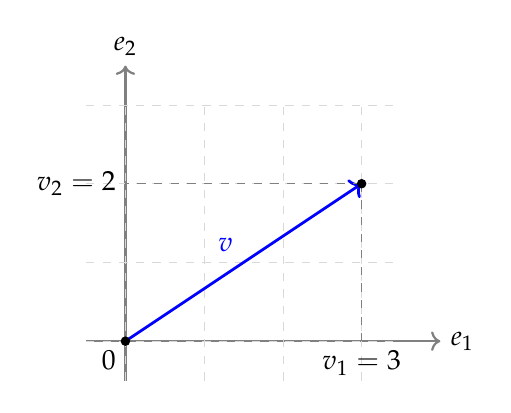
\begin{tikzpicture}[scale=1.0]
    % Coordinate axes
    \draw[->, thick, gray] (-0.5,0) -- (4,0) node[right, black] {$e_1$};
    \draw[->, thick, gray] (0,-0.5) -- (0,3.5) node[above, black] {$e_2$};
    
    % Grid
    \draw[help lines, color=gray!30, dashed] (-0.5,-0.5) grid (3.5,3);
    
    % Vector v = (3, 2)
    \draw[->, thick, blue, line width=1pt] (0,0) -- (3,2) 
        node[midway, above left] {$v$};
    
    % Components
    \draw[dashed, gray] (3,2) -- (3,0);
    \draw[dashed, gray] (3,2) -- (0,2);
    
    % Component labels
    \node[below] at (3,0) {$v_1 = 3$};
    \node[left] at (0,2) {$v_2 = 2$};
    
    % Origin
    \node[below left] at (0,0) {$0$};
    \filldraw (0,0) circle (1.5pt);
    \filldraw (3,2) circle (1.5pt);
    
\end{tikzpicture}
\caption{A vector $v = (3, 2)' \in \mathbb{R}^2$ visualised as an
arrow from the origin to the point with coordinates $v_1 = 3$ and
$v_2 = 2$.}
\label{fig:vector-2d}
\end{figure}

\paragraph{Length (norm) and inner product.}
Two operations on vectors are central to all linear algebra. The
\emph{Euclidean norm} of $v$ is the length of the corresponding
arrow:
\[
\|v\| \;=\; \sqrt{v_1^2 + v_2^2 + \cdots + v_n^2} \;=\; \sqrt{v' v}.
\]
The \emph{inner product} (or dot product) of two vectors
$u, v \in \mathbb{R}^n$ is the scalar
\[
u' v \;=\; u_1 v_1 + u_2 v_2 + \cdots + u_n v_n.
\]
The geometric meaning of the inner product is captured by the
identity $u' v = \|u\| \, \|v\| \cos\theta$, where $\theta$ is the
angle between the two vectors. Two consequences are particularly
useful: $u' v = 0$ if and only if $u$ and $v$ are \emph{orthogonal}
(perpendicular), and $u' v$ is positive (resp.\ negative) if the
angle between them is acute (resp.\ obtuse).

\paragraph{Vector addition and scalar multiplication.}
Two more operations complete the basic algebra. \emph{Addition} of
two vectors is component-wise: $u + v = (u_1 + v_1, \ldots, u_n + v_n)'$.
Geometrically, $u + v$ is the diagonal of the parallelogram formed by
$u$ and $v$. \emph{Scalar multiplication} of a vector by a real
number $c$ is also component-wise: $c\, v = (c v_1, \ldots, c v_n)'$.
Geometrically, multiplication by $c$ stretches or compresses $v$ by
the factor $|c|$, and reverses its direction if $c < 0$.

\begin{figure}[H]
\centering
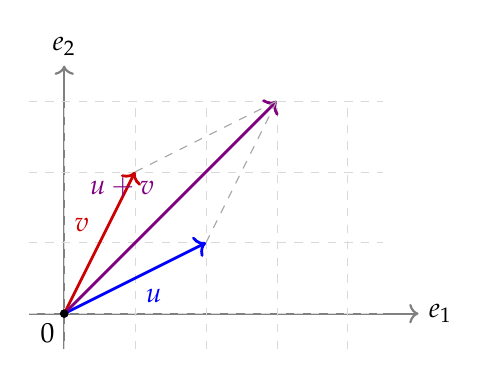
\begin{tikzpicture}[scale=0.9]
    % Coordinate axes
    \draw[->, thick, gray] (-0.5,0) -- (5,0) node[right, black] {$e_1$};
    \draw[->, thick, gray] (0,-0.5) -- (0,3.5) node[above, black] {$e_2$};
    
    % Grid
    \draw[help lines, color=gray!30, dashed] (-0.5,-0.5) grid (4.5,3);
    
    % Vector u = (2, 1)
    \draw[->, thick, blue, line width=1pt] (0,0) -- (2,1) 
        node[midway, below right] {$u$};
    
    % Vector v = (1, 2)
    \draw[->, thick, red!80!black, line width=1pt] (0,0) -- (1,2) 
        node[midway, above left] {$v$};
    
    % Sum u + v = (3, 3)
    \draw[->, thick, violet, line width=1pt] (0,0) -- (3,3) 
        node[midway, above left, xshift=-2pt] {$u + v$};
    
    % Parallelogram
    \draw[dashed, gray!70] (2,1) -- (3,3);
    \draw[dashed, gray!70] (1,2) -- (3,3);
    
    % Origin
    \node[below left] at (0,0) {$0$};
    \filldraw (0,0) circle (1.5pt);
    
\end{tikzpicture}
\caption{Addition of two vectors $u, v \in \mathbb{R}^2$. The sum
$u + v$ is the diagonal of the parallelogram spanned by $u$ and $v$.}
\label{fig:vector-addition}
\end{figure}

\paragraph{Standard basis and coordinates.}
The \emph{standard basis} of $\mathbb{R}^n$ is the set of $n$ unit
vectors $\{e_1, e_2, \ldots, e_n\}$, where each $e_i$ has a $1$ in
position $i$ and zeros elsewhere. Any vector $v \in \mathbb{R}^n$
admits the unique decomposition
\[
v \;=\; v_1\, e_1 \;+\; v_2\, e_2 \;+\; \cdots \;+\; v_n\, e_n,
\]
which expresses $v$ as a linear combination of the basis vectors with
coefficients equal to its coordinates. This decomposition is so
natural that we usually identify $v$ with its column of coordinates
$(v_1, \ldots, v_n)'$. However, it is important to keep in mind that
the coordinates depend on the chosen basis: in a different basis (for
instance, the basis of eigenvectors of a matrix, used extensively in
the spectral decomposition), the same vector $v$ has different
coordinates. The vector itself is a geometric object; its
coordinates are merely a representation in a specific reference
system.

\paragraph{Why vectors matter for the DFM.}
In the dynamic factor model, several objects are vectors of various
dimensions:
\begin{itemize}[leftmargin=1.5em, itemsep=2pt]
    \item the observation vector $y_t \in \mathbb{R}^M$, with one
          component per observed series at time $t$;
    \item the latent factor vector $f_t \in \mathbb{R}^r$, with one
          component per common factor;
    \item the augmented state vector
          $\tilde{f}_t = (f_t', f_{t-1}', \ldots, f_{t-4}')' \in \mathbb{R}^{5r}$,
          stacking the current and four lagged factors;
    \item the idiosyncratic shock $\varepsilon_t \in \mathbb{R}^M$
          and the factor innovation $u_t \in \mathbb{R}^r$, both
          vectors of suitable dimension.
\end{itemize}
Each of these vectors lives in its own Euclidean space, and the
geometric operations introduced in this section — norm, inner
product, addition — apply to all of them. The role of matrices, to
which we turn next, is to map vectors from one such space to another
and to encode the linear relationships among them.

\subsection{Matrices as Linear Transformations}
\label{sec:appendix-matrices}

Having introduced vectors as the basic geometric objects of
$\mathbb{R}^n$, we now turn to matrices. A matrix
$A \in \mathbb{R}^{m \times n}$ is a rectangular array of $mn$ real
numbers, organised in $m$ rows and $n$ columns:
\[
A \;=\; \begin{pmatrix}
a_{11} & a_{12} & \cdots & a_{1n} \\
a_{21} & a_{22} & \cdots & a_{2n} \\
\vdots & \vdots & \ddots & \vdots \\
a_{m1} & a_{m2} & \cdots & a_{mn}
\end{pmatrix}.
\]
Matrices admit two complementary readings, both of which will be
useful in what follows.

\paragraph{Matrices as collections of vectors.}
The first reading sees a matrix as a \emph{collection of vectors}.
Specifically, $A$ can be viewed either as a horizontal stack of $n$
column vectors $a_{\cdot 1}, a_{\cdot 2}, \ldots, a_{\cdot n} \in \mathbb{R}^m$,
\[
A \;=\; \big(\,a_{\cdot 1} \;\big|\; a_{\cdot 2} \;\big|\; \cdots \;\big|\; a_{\cdot n}\,\big),
\]
or as a vertical stack of $m$ row vectors $a_{1 \cdot}, a_{2 \cdot}, \ldots, a_{m \cdot} \in \mathbb{R}^{1 \times n}$.
This reading is particularly natural when the columns of $A$ have a
direct interpretation: in our DFM, for instance, the columns of the
loading matrix $\mL$ are the loadings of all $M$ observed series on
each individual factor, and the rows of $\mL$ are the loadings of
each individual series on all $r$ factors.

\paragraph{Matrices as linear transformations.}
The second, and more important, reading sees a matrix as a
\emph{linear transformation} from one Euclidean space to another. The
matrix $A \in \mathbb{R}^{m \times n}$ defines a function
$T_A: \mathbb{R}^n \to \mathbb{R}^m$ via
\[
T_A(v) \;=\; A v, \qquad v \in \mathbb{R}^n.
\]
The transformation $T_A$ is \emph{linear} in the sense that it
preserves vector addition and scalar multiplication:
\[
T_A(v + w) \;=\; T_A(v) + T_A(w), \qquad
T_A(c\, v) \;=\; c\, T_A(v).
\]
This linearity has a striking geometric consequence: $T_A$ maps the
origin to the origin, straight lines to straight lines, and parallel
lines to parallel lines. In particular, it maps the unit square (in
$\mathbb{R}^2$) to a parallelogram, and the unit cube (in
$\mathbb{R}^3$) to a parallelepiped — the shape is determined
entirely by the columns of $A$, which are the images of the standard
basis vectors $e_1, e_2, \ldots, e_n$. Indeed,
\[
A\, e_i \;=\; a_{\cdot i}, \qquad i = 1, 2, \ldots, n,
\]
so the $i$-th column of $A$ is precisely the image of the $i$-th
basis vector under $T_A$. This is the geometric meaning of the
columns of a matrix: \emph{they tell us where the basis vectors are
sent}, and the transformation of any other vector follows by
linearity.

\begin{figure}[H]
\centering
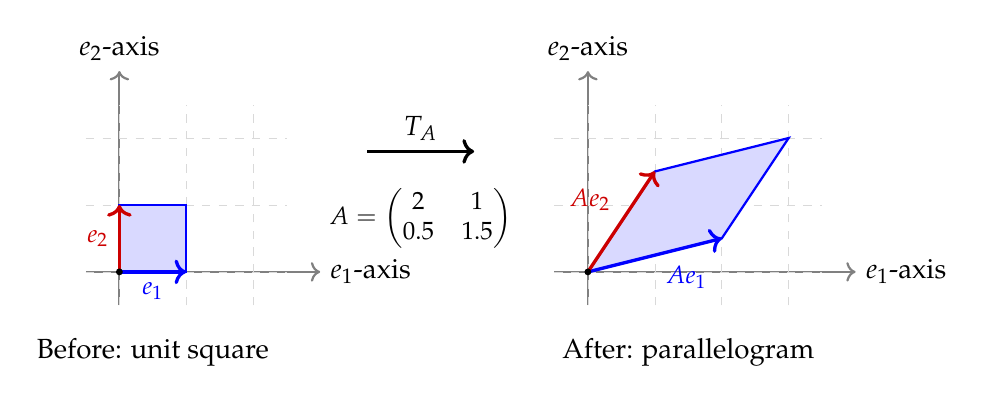
\begin{tikzpicture}[scale=0.85]
    % Left panel: original unit square with basis vectors
    \begin{scope}[shift={(-5,0)}]
        \draw[->, thick, gray] (-0.5,0) -- (3,0) node[right, black] {$e_1$-axis};
        \draw[->, thick, gray] (0,-0.5) -- (0,3) node[above, black] {$e_2$-axis};
        \draw[help lines, color=gray!30, dashed] (-0.5,-0.5) grid (2.5,2.5);
        
        % Unit square
        \filldraw[fill=blue!15, draw=blue, thick] (0,0) -- (1,0) -- (1,1) -- (0,1) -- cycle;
        
        % Basis vectors
        \draw[->, thick, blue, line width=1.2pt] (0,0) -- (1,0) 
            node[midway, below] {\small $e_1$};
        \draw[->, thick, red!80!black, line width=1.2pt] (0,0) -- (0,1) 
            node[midway, left] {\small $e_2$};
        
        \node at (0.5, -1.2) {Before: unit square};
        \filldraw (0,0) circle (1.2pt);
    \end{scope}
    
    % Arrow indicating transformation
    \draw[->, very thick, black] (-1.3, 1.8) -- (0.3, 1.8) 
        node[midway, above] {$T_A$};
    \node at (-0.5, 0.8) {\small $A = \begin{pmatrix} 2 & 1 \\ 0.5 & 1.5 \end{pmatrix}$};
    
    % Right panel: transformed parallelogram
    \begin{scope}[shift={(2,0)}]
        \draw[->, thick, gray] (-0.5,0) -- (4,0) node[right, black] {$e_1$-axis};
        \draw[->, thick, gray] (0,-0.5) -- (0,3) node[above, black] {$e_2$-axis};
        \draw[help lines, color=gray!30, dashed] (-0.5,-0.5) grid (3.5,2.5);
        
        % Transformed parallelogram (image of unit square under A)
        \filldraw[fill=blue!15, draw=blue, thick] 
            (0,0) -- (2,0.5) -- (3,2) -- (1,1.5) -- cycle;
        
        % Transformed basis vectors
        \draw[->, thick, blue, line width=1.2pt] (0,0) -- (2,0.5) 
            node[midway, below right] {\small $A e_1$};
        \draw[->, thick, red!80!black, line width=1.2pt] (0,0) -- (1,1.5) 
            node[midway, above left] {\small $A e_2$};
        
        \node at (1.5, -1.2) {After: parallelogram};
        \filldraw (0,0) circle (1.2pt);
    \end{scope}
\end{tikzpicture}
\caption{A linear transformation $T_A$ defined by a matrix
$A \in \mathbb{R}^{2 \times 2}$ maps the unit square (left) to a
parallelogram (right). The columns of $A$ are the images of the
standard basis vectors: $A e_1$ is the first column and $A e_2$ is
the second column. The transformation preserves the origin, parallel
lines, and ratios of lengths along any single direction.}
\label{fig:linear-transformation}
\end{figure}

\paragraph{Three special cases.}
A few elementary linear transformations are worth visualising
explicitly, because more general matrices can be understood by
combining them.

\emph{The identity matrix $I_n$} maps every vector to itself:
$T_{I_n}(v) = v$. The unit square is sent to itself, unchanged.

\emph{Diagonal matrices} apply independent stretching along each
coordinate axis. For $D = \mathrm{diag}(d_1, d_2)$, the
transformation $T_D$ sends the unit square to a rectangle of width
$d_1$ and height $d_2$ (or to a reflection, if some $d_i < 0$).
There is no rotation; only axis-aligned stretching.

\emph{Rotation matrices} preserve lengths and angles, rotating every
vector around the origin by a fixed angle $\theta$. In two
dimensions, the rotation matrix is
\[
R_\theta \;=\; \begin{pmatrix} \cos\theta & -\sin\theta \\ \sin\theta & \cos\theta \end{pmatrix}.
\]
The unit square is sent to another unit square, rotated by $\theta$.
No stretching, only rotation.

A general matrix $A \in \mathbb{R}^{2 \times 2}$ produces a
combination of these elementary operations: rotation, stretching, and
possibly reflection. The spectral decomposition of a symmetric
positive-definite matrix, derived in a later section, will make this
decomposition explicit.

\paragraph{Composition of transformations.}
If $A: \mathbb{R}^n \to \mathbb{R}^m$ and $B: \mathbb{R}^m \to \mathbb{R}^p$
are two linear transformations, their composition is itself linear
and is represented by the \emph{product matrix} $BA \in \mathbb{R}^{p \times n}$:
\[
T_B \circ T_A (v) \;=\; B (A v) \;=\; (BA)\, v.
\]
This is the source of the matrix-multiplication formula, which
encodes the algebraic rule for composing two linear maps. The order
matters: in general $AB \neq BA$, reflecting the fact that the order
in which two transformations are applied affects the final result.

\paragraph{Matrices in the DFM.}
The matrices appearing in the dynamic factor model can now be
interpreted as linear transformations on the relevant spaces.
\begin{itemize}[leftmargin=1.5em, itemsep=2pt]
    \item The loading matrix $\mL \in \mathbb{R}^{M \times r}$ is a
          map from the factor space $\mathbb{R}^r$ to the observation
          space $\mathbb{R}^M$, sending each factor configuration
          $f_t$ to its observation-space image $\mL f_t$.
    \item The transition matrix $\mathbf{A} \in \mathbb{R}^{r \times r}$
          is a map from the factor space to itself, propagating
          factors one step forward in time:
          $f_t \mapsto \mathbf{A} f_t$.
    \item The selection matrix $\mathbf{W}_t \in \{0,1\}^{m_t \times M}$
          is a projection from the full observation space onto the
          subspace of currently observed components.
\end{itemize}
The geometric perspective on matrices as transformations is the key
to making sense of these objects; the algebraic perspective on
matrices as collections of numbers gives us the operational tools to
compute with them.

\subsection{The Determinant as a Stretching Factor}
\label{sec:appendix-determinant}

The determinant of a square matrix has both an algebraic definition
and a geometric one. The algebraic definition — as a polynomial in
the matrix entries with specific sign properties — is computationally
useful but offers little intuition. The geometric definition — as a
\emph{volume scaling factor} — captures the meaning that we use
throughout the thesis.

\paragraph{Geometric definition.}
Let $A \in \mathbb{R}^{n \times n}$ be a square matrix, viewed as a
linear transformation $T_A: \mathbb{R}^n \to \mathbb{R}^n$. The
\emph{determinant} of $A$, denoted $\det(A)$ or $|A|$, is the factor
by which $T_A$ scales the volume of any region in $\mathbb{R}^n$.
Specifically, if $S \subset \mathbb{R}^n$ is a region of volume
$\mathrm{Vol}(S)$, then its image under $T_A$ has volume
\[
\mathrm{Vol}(T_A(S)) \;=\; |\det(A)| \cdot \mathrm{Vol}(S).
\]
The volume scaling factor is independent of the chosen region $S$ —
it depends only on the matrix. The sign of $\det(A)$ encodes
\emph{orientation}: $\det(A) > 0$ means $T_A$ preserves orientation
(does not perform a reflection), while $\det(A) < 0$ means $T_A$
reverses orientation (it includes a reflection). The absolute value
$|\det(A)|$ is the pure volume scaling.

\paragraph{The two-dimensional case.}
In two dimensions, the determinant has an especially clean
interpretation. Recall from the previous section that
$T_A$ maps the unit square (with vertices $0, e_1, e_1 + e_2, e_2$)
to a parallelogram with vertices $0, A e_1, A e_1 + A e_2, A e_2$.
The unit square has area $1$, so the parallelogram has area
$|\det(A)|$.

\begin{figure}[H]
\centering
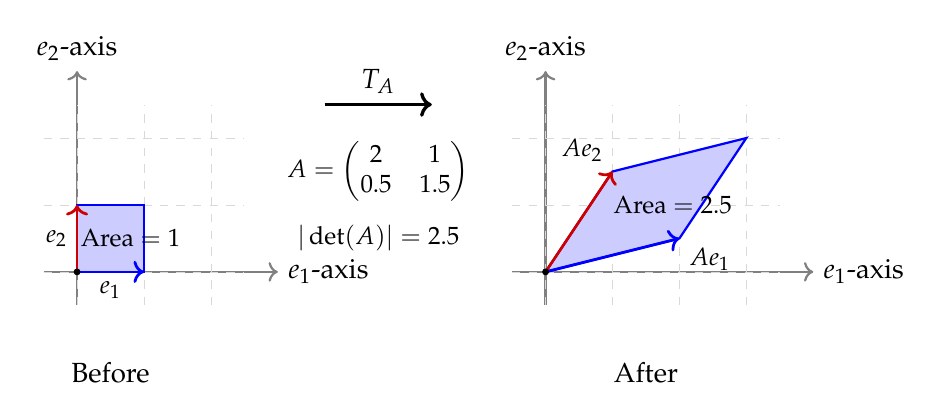
\begin{tikzpicture}[scale=0.85]
    % Left panel: unit square (area = 1)
    \begin{scope}[shift={(-5,0)}]
        \draw[->, thick, gray] (-0.5,0) -- (3,0) node[right, black] {$e_1$-axis};
        \draw[->, thick, gray] (0,-0.5) -- (0,3) node[above, black] {$e_2$-axis};
        \draw[help lines, color=gray!30, dashed] (-0.5,-0.5) grid (2.5,2.5);
        
        % Unit square
        \filldraw[fill=blue!20, draw=blue, thick] (0,0) -- (1,0) -- (1,1) -- (0,1) -- cycle;
        \node at (0.8, 0.5) {\small Area $= 1$};
        
        % Basis vectors
        \draw[->, thick, blue, line width=1pt] (0,0) -- (1,0);
        \draw[->, thick, red!80!black, line width=1pt] (0,0) -- (0,1);
        \node[below] at (0.5, 0) {\small $e_1$};
        \node[left] at (0, 0.5) {\small $e_2$};
        
        \node at (0.5, -1.5) {Before};
        \filldraw (0,0) circle (1.2pt);
    \end{scope}
    
    % Arrow indicating transformation (placed high)
    \draw[->, very thick, black] (-1.3, 2.5) -- (0.3, 2.5) 
        node[midway, above] {$T_A$};
    
    % Matrix label (placed in middle)
    \node at (-0.5, 1.5) {\small $A = \begin{pmatrix} 2 & 1 \\ 0.5 & 1.5 \end{pmatrix}$};
    
    % Determinant value (placed low)
    \node at (-0.5, 0.5) {\small $|\det(A)| = 2.5$};
    
    % Right panel: parallelogram (area = |det A| = 2.5)
    \begin{scope}[shift={(2,0)}]
        \draw[->, thick, gray] (-0.5,0) -- (4,0) node[right, black] {$e_1$-axis};
        \draw[->, thick, gray] (0,-0.5) -- (0,3) node[above, black] {$e_2$-axis};
        \draw[help lines, color=gray!30, dashed] (-0.5,-0.5) grid (3.5,2.5);
        
        % Transformed parallelogram
        \filldraw[fill=blue!20, draw=blue, thick] 
            (0,0) -- (2,0.5) -- (3,2) -- (1,1.5) -- cycle;
        \node at (1.9, 1) {\small Area $= 2.5$};
        
        % Transformed basis vectors
        \draw[->, thick, blue, line width=1pt] (0,0) -- (2,0.5);
        \draw[->, thick, red!80!black, line width=1pt] (0,0) -- (1,1.5);
        \node[below right] at (2, 0.5) {\small $A e_1$};
        \node[above left] at (1, 1.5) {\small $A e_2$};
        
        \node at (1.5, -1.5) {After};
        \filldraw (0,0) circle (1.2pt);
    \end{scope}
\end{tikzpicture}
\caption{Geometric meaning of the determinant. The matrix
$A = \begin{pmatrix} 2 & 1 \\ 0.5 & 1.5 \end{pmatrix}$ has
$\det(A) = 2 \cdot 1.5 - 1 \cdot 0.5 = 2.5$. The unit square (left,
area $1$) is mapped to a parallelogram (right, area $2.5$) — the
determinant is the area-scaling factor.}
\label{fig:determinant-stretching}
\end{figure}

\paragraph{Three special cases worth visualising.}

\emph{Case 1: $\det(A) > 1$ — expansion.} The transformation enlarges
volumes. Long vectors get longer, regions become bigger. This is the
case of the figure above, where a unit area is stretched into a
$2.5$-area parallelogram.

\emph{Case 2: $0 < \det(A) < 1$ — contraction.} The transformation
shrinks volumes. The unit square is mapped to a parallelogram of area
less than $1$. Notably, repeated application of $A$ produces
geometrically vanishing regions: $\det(A^k) = (\det A)^k \to 0$ as
$k \to \infty$.

\emph{Case 3: $\det(A) = 0$ — collapse.} The transformation collapses
the entire space to a lower-dimensional subspace. The unit square is
mapped to a line segment, or even to a single point. Geometrically,
the parallelogram \emph{degenerates}: two of its sides become
parallel (in 2D) and the area shrinks to zero. Algebraically, this
corresponds to the columns of $A$ being linearly dependent — they no
longer span the full space. A matrix with $\det(A) = 0$ is called
\emph{singular}, and its action is irreversible: distinct vectors can
be mapped to the same image, so $T_A$ cannot be inverted.

\begin{figure}[H]
\centering
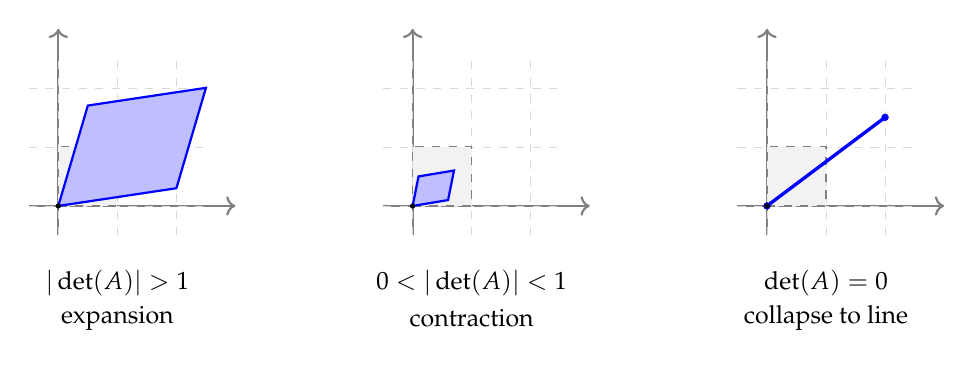
\begin{tikzpicture}[scale=0.75]
    % Three side-by-side panels showing the three cases
    
    % Panel 1: expansion
    \begin{scope}[shift={(-7,0)}]
        \draw[->, thick, gray] (-0.5,0) -- (3,0);
        \draw[->, thick, gray] (0,-0.5) -- (0,3);
        \draw[help lines, color=gray!30, dashed] (-0.5,-0.5) grid (2.5,2.5);
        
        % Original unit square (light)
        \draw[fill=gray!10, draw=gray, dashed] (0,0) -- (1,0) -- (1,1) -- (0,1) -- cycle;
        
        % Expanded parallelogram
        \filldraw[fill=blue!25, draw=blue, thick] 
            (0,0) -- (2,0.3) -- (2.5,2) -- (0.5,1.7) -- cycle;
        
        \filldraw (0,0) circle (1pt);
        \node at (1, -1.3) {\small $|\det(A)| > 1$};
        \node at (1, -1.9) {\small expansion};
    \end{scope}
    
    % Panel 2: contraction
    \begin{scope}[shift={(-1,0)}]
        \draw[->, thick, gray] (-0.5,0) -- (3,0);
        \draw[->, thick, gray] (0,-0.5) -- (0,3);
        \draw[help lines, color=gray!30, dashed] (-0.5,-0.5) grid (2.5,2.5);
        
        % Original unit square (light)
        \draw[fill=gray!10, draw=gray, dashed] (0,0) -- (1,0) -- (1,1) -- (0,1) -- cycle;
        
        % Contracted parallelogram
        \filldraw[fill=blue!25, draw=blue, thick] 
            (0,0) -- (0.6,0.1) -- (0.7,0.6) -- (0.1,0.5) -- cycle;
        
        \filldraw (0,0) circle (1pt);
        \node at (1, -1.3) {\small $0 < |\det(A)| < 1$};
        \node at (1, -1.9) {\small contraction};
    \end{scope}
    
    % Panel 3: collapse (det = 0)
    \begin{scope}[shift={(5,0)}]
        \draw[->, thick, gray] (-0.5,0) -- (3,0);
        \draw[->, thick, gray] (0,-0.5) -- (0,3);
        \draw[help lines, color=gray!30, dashed] (-0.5,-0.5) grid (2.5,2.5);
        
        % Original unit square (light)
        \draw[fill=gray!10, draw=gray, dashed] (0,0) -- (1,0) -- (1,1) -- (0,1) -- cycle;
        
        % Collapsed (line segment)
        \draw[blue, very thick] (0,0) -- (2,1.5);
        \filldraw[blue] (0,0) circle (1.5pt);
        \filldraw[blue] (2,1.5) circle (1.5pt);
        
        \filldraw (0,0) circle (1pt);
        \node at (1, -1.3) {\small $\det(A) = 0$};
        \node at (1, -1.9) {\small collapse to line};
    \end{scope}
\end{tikzpicture}
\caption{Three regimes of the determinant. From left to right:
expansion ($|\det(A)| > 1$), contraction ($|\det(A)| < 1$), and
collapse to a lower-dimensional subspace ($\det(A) = 0$, the
singular case). The original unit square is shown in dashed grey for
reference.}
\label{fig:determinant-three-cases}
\end{figure}

\paragraph{Algebraic computation.}
For practical computations, the determinant of a $2 \times 2$ matrix is
\[
\det\!\begin{pmatrix} a & b \\ c & d \end{pmatrix} \;=\; ad - bc.
\]
For larger matrices, the determinant can be computed via cofactor
expansion (recursive but expensive for $n > 4$) or via
LU-decomposition (much faster, $O(n^3)$). Three properties are used
repeatedly throughout the thesis:
\begin{itemize}[leftmargin=1.5em, itemsep=2pt]
    \item \emph{Multiplicativity}: $\det(AB) = \det(A) \det(B)$ for any
          two square matrices of the same size.
    \item \emph{Inverse}: $\det(A^{-1}) = 1/\det(A)$, valid whenever
          $\det(A) \neq 0$.
    \item \emph{Diagonal and triangular matrices}: the determinant is
          the product of the diagonal entries. In particular, for
          $D = \mathrm{diag}(d_1, \ldots, d_n)$,
          $\det(D) = d_1 d_2 \cdots d_n$.
\end{itemize}

\paragraph{Why the determinant matters in the DFM.}
The determinant appears repeatedly in the thesis through the
multivariate Gaussian and Student-$t$ densities. The normalising
constant of $\mathcal{N}(\mu, \Sigma)$ in $m$ dimensions involves
$|\Sigma|^{1/2}$, which — by the volume interpretation derived in
the Geometric Interlude — is
proportional to the volume of the Mahalanobis ellipsoid
$\{x : (x-\mu)'\Sigma^{-1}(x-\mu) \leq 1\}$. A large $|\Sigma|$ means
a large ellipsoid, hence a flat density; a small $|\Sigma|$ means a
concentrated ellipsoid, hence a peaked density. In the M-step
derivations, the term $-\tfrac{T}{2}\log|\Sigma|$ that appears in the
expected complete-data log-likelihood is precisely a penalty against
distributions whose ellipsoid is too large — the algorithm balances
the fit quality (driven by Mahalanobis distances of the residuals)
against this volumetric penalty.

\subsection{Eigenvalues and Eigenvectors: A Visual Introduction}
\label{sec:appendix-eigen-visual}

We now arrive at the central concept of this appendix: eigenvalues
and eigenvectors. Their formal treatment will be developed in detail
in the next section; here we focus on the geometric intuition,
visualising what eigenvectors and eigenvalues look like in two
dimensions.

\paragraph{The defining property.}
A non-zero vector $v \in \mathbb{R}^n$ is called an
\emph{eigenvector} of a square matrix $A \in \mathbb{R}^{n \times n}$
if its image $A v$ lies on the same line as $v$. Equivalently, there
exists a scalar $\lambda$ such that
\[
A v \;=\; \lambda\, v.
\]
The scalar $\lambda$ is the \emph{eigenvalue} corresponding to $v$.
The defining condition has a vivid geometric interpretation: an
eigenvector is a direction in which $A$ acts by \emph{pure
stretching}, with no rotation. Most directions in space are
\emph{not} eigendirections — they get both rotated and stretched by
$A$. Eigendirections are the special, privileged directions in which
the action of $A$ simplifies to a scalar multiplication.

\begin{figure}[H]
\centering
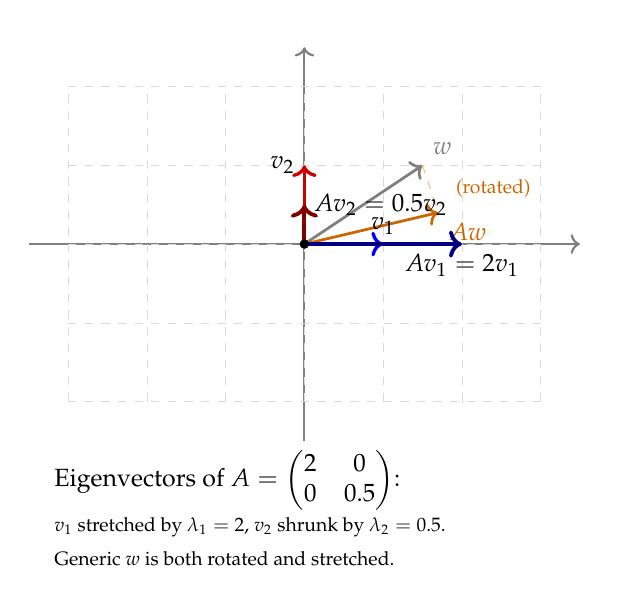
\begin{tikzpicture}[scale=1.0]
    \draw[->, thick, gray] (-3.5,0) -- (3.5,0) node[right, black] {};
    \draw[->, thick, gray] (0,-2.5) -- (0,2.5) node[above, black] {};
    \draw[help lines, color=gray!30, dashed] (-3,-2) grid (3,2);
    
    % Generic vector (gets rotated)
    \draw[->, thick, gray, line width=1pt] (0,0) -- (1.5,1) 
        node[above right] {\small $w$};
    \draw[->, thick, orange!80!black, line width=1pt] (0,0) -- (1.7,0.4) 
        node[below right] {\small $A w$};
    \draw[dashed, orange!50, thin] (1.5,1) -- (1.7,0.4);
    \node[orange!80!black, font=\scriptsize] at (2.4, 0.7) {(rotated)};
    
    % Eigenvector along x-axis with eigenvalue 2
    \draw[->, thick, blue, line width=1.2pt] (0,0) -- (1,0);
    \node[above] at (1,0) {\small $v_1$};
    \draw[->, thick, blue!50!black, line width=1.4pt] (0,0) -- (2,0);
    \node[below] at (2,0) {\small $A v_1 = 2 v_1$};
    
    % Eigenvector along y-axis with eigenvalue 0.5
    \draw[->, thick, red!80!black, line width=1.2pt] (0,0) -- (0,1);
    \node[left] at (0,1) {\small $v_2$};
    \draw[->, thick, red!50!black, line width=1.4pt] (0,0) -- (0,0.5);
    \node[right] at (0,0.5) {\small $A v_2 = 0.5 v_2$};
    
    \filldraw (0,0) circle (1.5pt);
    
    % Caption inside picture for clarity
    \node[font=\small, anchor=west] at (-3.3, -3) 
        {Eigenvectors of $A = \begin{pmatrix} 2 & 0 \\ 0 & 0.5 \end{pmatrix}$:};
    \node[font=\scriptsize, anchor=west] at (-3.3, -3.6) 
        {$v_1$ stretched by $\lambda_1 = 2$, $v_2$ shrunk by $\lambda_2 = 0.5$.};
    \node[font=\scriptsize, anchor=west] at (-3.3, -4.0) 
        {Generic $w$ is both rotated and stretched.};
\end{tikzpicture}
\caption{Eigenvectors as ``privileged directions'' under a linear
transformation. The matrix $A = \mathrm{diag}(2, 0.5)$ has the
coordinate axes as eigendirections: $v_1 = e_1$ is stretched by
$\lambda_1 = 2$, and $v_2 = e_2$ is shrunk by $\lambda_2 = 0.5$. A
generic vector $w$ that is not aligned with the eigenvectors is both
rotated and stretched by $A$.}
\label{fig:eigenvectors-visual}
\end{figure}

\paragraph{Why eigendirections are special.}
The previous figure displays a particularly simple case: $A$ is
diagonal, so the eigenvectors are the coordinate axes. For a generic
matrix $A$, the eigenvectors will \emph{not} coincide with the
coordinate axes — they will be rotated. The key insight is that
\emph{some} pair of perpendicular directions (in the symmetric case)
or \emph{some} pair of directions (in the general case) does play
the role of the coordinate axes: those are the eigendirections.

\begin{figure}[H]
\centering
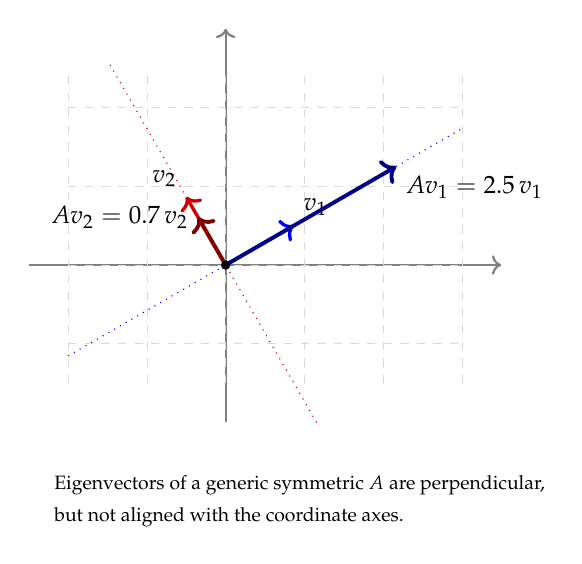
\begin{tikzpicture}[scale=1.0]
    \draw[->, thick, gray] (-2.5,0) -- (3.5,0);
    \draw[->, thick, gray] (0,-2) -- (0,3);
    \draw[help lines, color=gray!30, dashed] (-2,-1.5) grid (3,2.5);
    
    % First eigenvector at 30 degrees (length 1)
    \draw[->, thick, blue, line width=1.2pt] (0,0) -- (0.866, 0.5);
    \node[above right] at (0.866, 0.5) {\small $v_1$};
    
    % Stretched first eigenvector (lambda = 2.5)
    \draw[->, thick, blue!50!black, line width=1.4pt] (0,0) -- (2.165, 1.25);
    \node[below right] at (2.165, 1.25) {\small $A v_1 = 2.5\, v_1$};
    
    % Second eigenvector perpendicular (-sin(30), cos(30)) = (-0.5, 0.866)
    \draw[->, thick, red!80!black, line width=1.2pt] (0,0) -- (-0.5, 0.866);
    \node[above left] at (-0.5, 0.866) {\small $v_2$};
    
    % Stretched second eigenvector (lambda = 0.7)
    \draw[->, thick, red!50!black, line width=1.4pt] (0,0) -- (-0.35, 0.606);
    \node[left] at (-0.35, 0.606) {\small $A v_2 = 0.7\, v_2$};
    
    % Eigenvector lines (extended)
    \draw[blue, dotted, thin] (-2,-1.155) -- (3, 1.732);
    \draw[red!80!black, dotted, thin] (1.155, -2) -- (-1.5, 2.598);
    
    \filldraw (0,0) circle (1.5pt);
    
    \node[font=\scriptsize, anchor=west] at (-2.3, -2.8) 
        {Eigenvectors of a generic symmetric $A$ are perpendicular,};
    \node[font=\scriptsize, anchor=west] at (-2.3, -3.2) 
        {but not aligned with the coordinate axes.};
\end{tikzpicture}
\caption{For a generic symmetric matrix $A$, the eigenvectors $v_1,
v_2$ are perpendicular to each other (a property guaranteed by the
spectral theorem) but rotated relative to the coordinate axes. The
matrix $A$ stretches space along $v_1$ by $\lambda_1$ and along
$v_2$ by $\lambda_2$. The dotted lines indicate the eigendirections,
which form a rotated coordinate system in which $A$ acts diagonally.}
\label{fig:eigenvectors-rotated}
\end{figure}

\paragraph{Eigenvectors and the spectral decomposition.}
The fact that perpendicular eigenvectors exist for any symmetric
matrix is the content of the \emph{spectral theorem}, which we state
formally in the next section. For now, the geometric picture is
sufficient: the spectral decomposition $\Sigma = V \Lambda V'$ that
we introduced in the Geometric Interlude is exactly the algebraic
expression of this geometric fact — $V$ is the matrix whose columns
are the eigenvectors, $\Lambda$ is the diagonal matrix of
eigenvalues, and the product $V \Lambda V'$ describes the
transformation as ``rotate to the eigenvector basis, stretch by the
eigenvalues, rotate back''.

\paragraph{Three regimes for two-dimensional eigenvalues.}
The qualitative behaviour of $A$ as a transformation depends on the
sign and magnitude of its eigenvalues. Three regimes are worth
visualising:
\begin{itemize}[leftmargin=1.5em, itemsep=3pt]
    \item \emph{Both $\lambda_1, \lambda_2 > 1$}: pure expansion in
          both eigendirections. The unit square in the eigenvector
          basis is stretched into a larger rectangle.
    \item \emph{Both $0 < \lambda_1, \lambda_2 < 1$}: pure
          contraction. Repeated application of $A^k$ shrinks every
          vector to zero.
    \item \emph{$\lambda_1 > 1 > \lambda_2 > 0$}: stretching in one
          direction, compression in the other. This is the typical
          regime of empirical covariance matrices: most variance
          concentrates in a few principal directions, with the
          remaining directions carrying very little variance.
\end{itemize}

The third regime is particularly important for our setting: when we
apply PCA to macroeconomic data, the empirical covariance matrix
$\widehat{\boldsymbol{\Sigma}}_Y$ typically has a few large
eigenvalues (corresponding to common factors) and many small
eigenvalues (corresponding to idiosyncratic noise), exactly the
configuration of one stretched direction and many compressed
directions.

\paragraph{Towards the formal treatment.}
The visual intuition developed in this section is the geometric core
of the appendix that follows. The next section formalises the
spectral decomposition, derives its algebraic consequences (powers,
inverses, square roots of matrices), and connects eigenvalues to
positive definiteness, ellipsoids, and the volumetric meaning of the
determinant — all of which we have already used informally in the
Geometric Interlude. The remaining sections of the appendix then
apply these tools to specific problems: stability of linear
dynamical systems (the unit-circle condition for the VAR transition
matrix $\mathbf{A}$), Principal Component Analysis (eigendecomposition
of the sample covariance), and noise floors of random matrices (the
Circular and Marchenko–Pastur laws).

\subsection{Symmetric Positive-Definite Matrices and Ellipsoids}
\label{sec:appendix-ellipsoid}

A particularly important class of symmetric matrices is that of
\emph{positive-definite} (PD) matrices. A symmetric matrix
$\Sigma \in \mathbb{R}^{m \times m}$ is positive definite if
\[
v' \Sigma\, v \;>\; 0 \qquad \text{for every non-zero } v \in \mathbb{R}^m.
\]
Geometrically, this condition says that the quadratic form
$v \mapsto v' \Sigma v$ takes positive values everywhere except at
the origin. The level sets of this quadratic form are
\emph{ellipsoids} centred at the origin, and their geometry is
entirely controlled by the eigenstructure of $\Sigma$.

\paragraph{Eigenvalues of a PD matrix are positive.}
Suppose $v$ is an eigenvector of $\Sigma$ with eigenvalue $\lambda$.
Then $\Sigma v = \lambda v$, and
\[
v' \Sigma\, v \;=\; \lambda\, \|v\|^2.
\]
Since $v' \Sigma v > 0$ by positive definiteness and
$\|v\|^2 > 0$ for any non-zero vector, we must have $\lambda > 0$.
The same argument in reverse shows the converse: a symmetric matrix
with all positive eigenvalues is PD. So, for symmetric matrices,
\emph{positive definiteness is equivalent to all eigenvalues being
positive}.

\paragraph{The ellipsoid associated with $\Sigma$.}
Recall from the Geometric Interlude that the level set of the
Mahalanobis distance,
\[
E_c \;\equiv\; \{x \in \mathbb{R}^m : x' \Sigma^{-1} x \leq c\},
\]
is an ellipsoid centred at the origin. Using the spectral
decomposition $\Sigma = V \Lambda V'$ and the change of variable
$y = V' x$, this ellipsoid takes the equivalent form
\[
\sum_{i=1}^m \frac{y_i^2}{\lambda_i} \;\leq\; c.
\]
This is the standard form of an ellipsoid with axes along the
coordinate directions $y_1, \ldots, y_m$ and semi-axis lengths
$\sqrt{c\, \lambda_1}, \ldots, \sqrt{c\, \lambda_m}$. Going back to
the original coordinates via $x = V y$, the axes of $E_c$ are aligned
with the eigenvectors of $\Sigma$, and their semi-axis lengths are
$\sqrt{c\, \lambda_i}$.

\paragraph{Visualising the ellipsoid in two dimensions.}
In two dimensions, the ellipsoid is an ordinary ellipse. Its
geometric properties can be read directly off the spectral
decomposition of $\Sigma$:
\begin{itemize}[leftmargin=1.5em, itemsep=2pt]
    \item The \emph{orientation} of the ellipse is given by the
          eigenvectors $v_1, v_2$;
    \item The \emph{semi-axis lengths} are
          $\sqrt{\lambda_1}, \sqrt{\lambda_2}$ (taking $c = 1$);
    \item The \emph{eccentricity} (how elongated the ellipse is) is
          determined by the ratio $\lambda_1/\lambda_2$.
\end{itemize}

\begin{figure}[H]
\centering
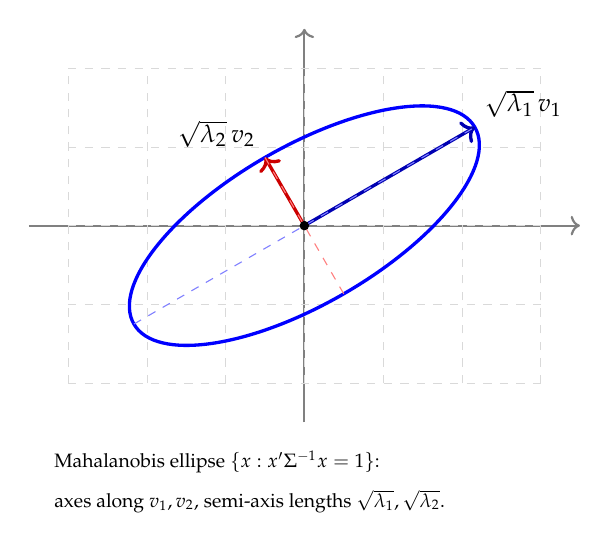
\begin{tikzpicture}[scale=1.0]
    \draw[->, thick, gray] (-3.5,0) -- (3.5,0);
    \draw[->, thick, gray] (0,-2.5) -- (0,2.5);
    \draw[help lines, color=gray!30, dashed] (-3,-2) grid (3,2);
    
    % Rotated ellipse (rotation 30 degrees, semi-axes 2.5 and 1)
    \draw[blue, very thick, rotate=30] (0,0) ellipse (2.5 and 1);
    
    % Eigenvectors (length sqrt(lambda))
    % v1 at 30 degrees, length sqrt(lambda1) = 2.5: (2.165, 1.25)
    \draw[->, thick, blue!70!black, line width=1.2pt] (0,0) -- (2.165, 1.25);
    \node[above right] at (2.165, 1.25) {\small $\sqrt{\lambda_1}\, v_1$};
    
    % v2 at 120 degrees, length sqrt(lambda2) = 1: (-0.5, 0.866)
    \draw[->, thick, red!80!black, line width=1.2pt] (0,0) -- (-0.5, 0.866);
    \node[above left] at (-0.5, 0.866) {\small $\sqrt{\lambda_2}\, v_2$};
    
    % Negative eigenvectors (just lines)
    \draw[blue!50, dashed, thin] (-2.165, -1.25) -- (2.165, 1.25);
    \draw[red!50, dashed, thin] (0.5, -0.866) -- (-0.5, 0.866);
    
    \filldraw (0,0) circle (1.5pt);
    
    \node[font=\scriptsize, anchor=west] at (-3.3, -3) 
        {Mahalanobis ellipse $\{x : x' \Sigma^{-1} x = 1\}$:};
    \node[font=\scriptsize, anchor=west] at (-3.3, -3.5) 
        {axes along $v_1, v_2$, semi-axis lengths $\sqrt{\lambda_1}, \sqrt{\lambda_2}$.};
\end{tikzpicture}
\caption{The Mahalanobis ellipse associated with a symmetric
positive-definite matrix $\Sigma$. The principal axes of the ellipse
are aligned with the eigenvectors $v_1, v_2$ of $\Sigma$, and the
semi-axis lengths are the square roots of the corresponding
eigenvalues. A large eigenvalue produces a long axis (high variance
in that direction); a small eigenvalue produces a short axis (low
variance in that direction).}
\label{fig:ellipsoid}
\end{figure}

\paragraph{Why $\sqrt{\lambda_i}$ and not $\lambda_i$?}
The square root in the semi-axis length is initially counterintuitive
but becomes clear with the following calculation. The eigenvalue
equation $\Sigma v_i = \lambda_i v_i$ shows that $\Sigma$ stretches
$v_i$ by a factor $\lambda_i$. The quadratic form $v' \Sigma v$, when
evaluated at the eigenvector, gives
$v_i' \Sigma v_i = \lambda_i \|v_i\|^2 = \lambda_i$ (assuming
$\|v_i\| = 1$). So a unit displacement along $v_i$ contributes
$\lambda_i$ to the quadratic form. To reach the level set
$x' \Sigma^{-1} x = 1$, we need a displacement of length
$\sqrt{\lambda_i}$ along $v_i$ — because the inverse $\Sigma^{-1}$
contracts by $1/\lambda_i$ in that direction. The square root is
therefore the natural ``half-length'' associated with the eigenvalue,
and it is the right measure of dispersion in the corresponding
principal direction.

\paragraph{Special cases worth visualising.}

\emph{Case 1: $\Sigma = \sigma^2 I_2$ (isotropic).} Both eigenvalues
equal $\sigma^2$, eigenvectors are arbitrary (any orthonormal basis
works), and the ellipse degenerates to a \emph{circle} of radius
$\sigma$. The distribution is equally spread in all directions.

\emph{Case 2: $\Sigma$ diagonal but unequal entries.} Eigenvectors are
the coordinate axes; semi-axis lengths are $\sqrt{\Sigma_{11}}$ and
$\sqrt{\Sigma_{22}}$. The ellipse is axis-aligned but elongated.

\emph{Case 3: $\Sigma$ with non-zero off-diagonals.} The eigenvectors
are rotated relative to the coordinate axes (the angle is determined
by the off-diagonal entries), and the ellipse is correspondingly
tilted. This is the case shown in Figure~\ref{fig:ellipsoid}.

\paragraph{Connection with the DFM.}
The scale matrix $\mathbf{Q}$ of the factor innovations and the scale
matrix $\mathbf{R}$ of the idiosyncratic shocks are both symmetric
and positive definite. Their ellipsoids describe the geometry of the
corresponding distributions: a large eigenvalue of $\mathbf{Q}$ in
some direction means that the factor innovation is volatile in that
direction; a large eigenvalue of $\mathbf{R}$ for some series means
that the idiosyncratic shock for that series is large. The smoothed
posterior covariance $P_{t \mid T}$ produced by the Kalman filter is
also a PD ellipsoid, this time describing the posterior uncertainty
about the factor at time $t$ — small eigenvalues mean tight
identification, large eigenvalues mean weak identification. The
distinction between scale and covariance is relevant when $\nu < \infty$:
in the Student-$t$ scale-mixture representation, $\mathbf{Q}$ and
$\mathbf{R}$ are scale matrices, and the actual covariance matrices
are $\tfrac{\nu_u}{\nu_u - 2}\mathbf{Q}$ and
$\tfrac{\nu_\varepsilon}{\nu_\varepsilon - 2}\mathbf{R}$ respectively
(when $\nu > 2$). The geometric interpretation in terms of ellipsoids
applies equally to both: covariance and scale ellipsoids differ only
by a uniform inflation factor in each dimension.

\subsection{The Mahalanobis Distance: A Visual Perspective}
\label{sec:appendix-mahalanobis}

The Mahalanobis distance was introduced algebraically in the
Geometric Interlude and used
extensively throughout the EM derivations. We now give it a
complementary visual treatment.

\paragraph{The Euclidean distance: a benchmark.}
Recall the ordinary Euclidean distance between $x$ and $\mu$:
\[
d_E(x, \mu) \;=\; \|x - \mu\| \;=\; \sqrt{(x - \mu)' (x - \mu)}.
\]
The level sets of $d_E$ are \emph{circles} (or spheres in higher
dimensions) centred at $\mu$. All points equidistant from $\mu$ lie
on the same circle; the circles get larger as $d_E$ increases. This
is the geometry of the standard isotropic Gaussian
$\mathcal{N}(\mu, I_m)$.

\paragraph{The Mahalanobis distance: a stretched and rotated alternative.}
The Mahalanobis distance generalises the Euclidean distance by
incorporating the scale matrix $\Sigma$:
\[
d_M(x, \mu; \Sigma) \;=\; \sqrt{(x - \mu)' \Sigma^{-1} (x - \mu)}.
\]
When $\Sigma = I_m$, the Mahalanobis distance reduces to the
Euclidean distance. For general $\Sigma$, the level sets of $d_M$
are no longer circles but \emph{ellipsoids} — exactly the ones
discussed in the previous section. Two points equidistant from $\mu$
in the Mahalanobis sense lie on the same ellipsoid; points along
the long axis of the ellipsoid are ``Mahalanobis-far'' even if they
are Euclidean-near.

\paragraph{Why this difference matters.}
The intuition is that the Mahalanobis distance \emph{accounts for the
shape of the distribution}. If $\Sigma$ has a large eigenvalue along
some direction (say, the $v_1$ direction), then movements along
$v_1$ are ``cheap'' — they cover little Mahalanobis ground because
the distribution is spread out in that direction, so a large
displacement is unsurprising. Conversely, movements perpendicular
to $v_1$ — along the short axis of the ellipsoid — are
``expensive'': they cover a lot of Mahalanobis ground per unit of
Euclidean distance, because the distribution is tightly concentrated
in that direction.

\begin{figure}[H]
\centering
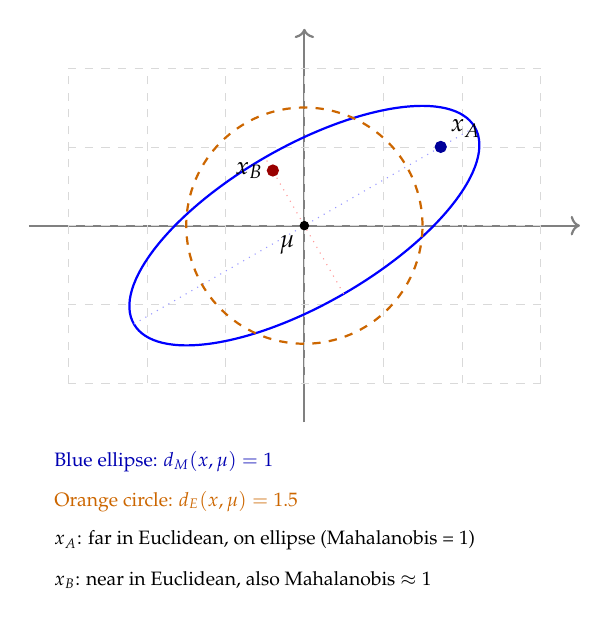
\begin{tikzpicture}[scale=1.0]
    \draw[->, thick, gray] (-3.5,0) -- (3.5,0);
    \draw[->, thick, gray] (0,-2.5) -- (0,2.5);
    \draw[help lines, color=gray!30, dashed] (-3,-2) grid (3,2);
    
    % Mahalanobis ellipse (level set d_M = 1)
    \draw[blue, thick, rotate=30] (0,0) ellipse (2.5 and 1);
    
    % Euclidean circle of radius 1.5
    \draw[orange!80!black, thick, dashed] (0,0) circle (1.5);
    
    % Eigenvector dotted lines
    \draw[blue!40, dotted, thin] (-2.165, -1.25) -- (2.165, 1.25);
    \draw[red!40, dotted, thin] (0.5, -0.866) -- (-0.5, 0.866);
    
    % Point A: along long axis (Mahalanobis-near, Euclidean-far)
    \filldraw[blue!60!black] (1.732, 1) circle (2pt);
    \node[above right] at (1.732, 1) {\small $x_A$};
    
    % Point B: along short axis (Mahalanobis-far, Euclidean-near)  
    \filldraw[red!60!black] (-0.4, 0.7) circle (2pt);
    \node[left] at (-0.4, 0.7) {\small $x_B$};
    
    \filldraw (0,0) circle (1.5pt);
    \node[below left] at (0,0) {\small $\mu$};
    
    \node[font=\scriptsize, blue!70!black, anchor=west] at (-3.3, -3) 
        {Blue ellipse: $d_M(x, \mu) = 1$};
    \node[font=\scriptsize, orange!80!black, anchor=west] at (-3.3, -3.5) 
        {Orange circle: $d_E(x, \mu) = 1.5$};
    \node[font=\scriptsize, anchor=west] at (-3.3, -4) 
        {$x_A$: far in Euclidean, on ellipse (Mahalanobis = 1)};
    \node[font=\scriptsize, anchor=west] at (-3.3, -4.5) 
        {$x_B$: near in Euclidean, also Mahalanobis $\approx 1$};
\end{tikzpicture}
\caption{Comparison of Euclidean and Mahalanobis distances. The
orange dashed circle is a level set of the Euclidean distance from
$\mu$. The blue ellipse is a level set of the Mahalanobis distance
under a non-isotropic $\Sigma$. Two points $x_A$ and $x_B$ at
similar Mahalanobis distance from $\mu$ can be at very different
Euclidean distances: $x_A$ is far Euclidean-wise but ``cheap''
Mahalanobis-wise (because it lies along the long axis of the
ellipse), whereas $x_B$ is close Euclidean-wise but ``expensive''
Mahalanobis-wise (because it lies along the short axis).}
\label{fig:mahalanobis}
\end{figure}

\paragraph{Whitening transformation: making Mahalanobis Euclidean.}
The Mahalanobis distance can be reduced to a Euclidean distance via
a coordinate change. Define the \emph{whitening transformation}
$z = \Sigma^{-1/2}(x - \mu)$, where $\Sigma^{-1/2}$ is the symmetric
inverse square root of $\Sigma$. Then
\[
\|z\|^2 \;=\; (x - \mu)'\, \Sigma^{-1/2} \, \Sigma^{-1/2} \,(x - \mu) \;=\; (x - \mu)' \Sigma^{-1} (x - \mu),
\]
so the Euclidean norm of $z$ equals the squared Mahalanobis distance
of $x$ from $\mu$. Geometrically, $\Sigma^{-1/2}$ is the linear
transformation that rotates the eigenvectors of $\Sigma$ to the
coordinate axes \emph{and} contracts each axis by $1/\sqrt{\lambda_i}$,
turning the ellipsoid into a unit circle. In this transformed
``whitened'' space, the Mahalanobis distance is just the ordinary
Euclidean distance, and the distribution is just the standard
isotropic Gaussian.

\paragraph{Why this matters in the EM derivations.}
The Mahalanobis distance appears throughout the M-step in two
distinct forms.

First, as the \emph{quadratic kernel} of the Gaussian/Student-$t$
density: $-\tfrac{1}{2}(x-\mu)'\Sigma^{-1}(x-\mu)$ in the Gaussian
log-density, polynomial in the Student-$t$ case. The expected value
of this quantity, taken over the posterior of the latent variables,
drives the M-step updates of the loading matrix $\mL$ and the
transition matrix $\mathbf{A}$.

Second, as the \emph{weight assignment rule} in the Student-$t$
scale-mixture representation. The posterior weight
$\hat{w}_t = (\nu + p)/(\nu + d_t)$ for an observation depends on
its Mahalanobis distance $d_t$ from the centre: observations with
small $d_t$ (near the centre of the ellipsoid) receive weights near
$1$; observations with large $d_t$ (in the tails of the ellipsoid)
are down-weighted with $\hat{w}_t \to 0$. The Mahalanobis distance
is therefore the geometric quantity that the algorithm uses to
decide which observations to ``trust'' and which to discount as
outliers.

\subsection{Volumes, Determinants, and the Geometry of Concentration}
\label{sec:appendix-volume}

We have seen that the determinant of a matrix is a volume-scaling
factor, and that the
Mahalanobis ellipsoid associated with a covariance matrix $\Sigma$
has axes determined by the eigenvectors of $\Sigma$ and semi-axis
lengths $\sqrt{\lambda_i}$.
We now connect these two facts: the volume of the Mahalanobis
ellipsoid is determined by $|\Sigma|^{1/2}$, and the determinant
$|\Sigma|$ is therefore a measure of \emph{how spread out} the
distribution is.

\paragraph{The volume of a 2D ellipse.}
In two dimensions, the area of an ellipse with semi-axis lengths $a$
and $b$ is
\[
\mathrm{Area} \;=\; \pi\, a\, b.
\]
For the Mahalanobis ellipse $\{x : x' \Sigma^{-1} x \leq 1\}$, the
semi-axis lengths are $a = \sqrt{\lambda_1}$ and $b = \sqrt{\lambda_2}$,
so
\[
\mathrm{Area}(E_1) \;=\; \pi\, \sqrt{\lambda_1 \lambda_2} \;=\; \pi\, \sqrt{|\Sigma|}.
\]
The area of the unit Mahalanobis ellipse is therefore proportional
to $\sqrt{|\Sigma|}$, with $\pi$ as the proportionality constant.

\paragraph{Why $|\Sigma| = \prod_i \lambda_i$.}
The identity $|\Sigma| = \lambda_1 \lambda_2 \cdots \lambda_m$ is a
general property of any square matrix: the determinant equals the
product of the eigenvalues, counted with multiplicity. For a
symmetric positive-definite $\Sigma$, this identity has two
particularly clean consequences. First, all $\lambda_i > 0$, so
$|\Sigma| > 0$ — the determinant is strictly positive (and not just
non-zero), and $|\Sigma|^{1/2} = \sqrt{\lambda_1 \cdots \lambda_m}$
is well-defined as a real number without any sign or branch
ambiguity. Second, the level set
$\{x : x'\Sigma^{-1}x \leq 1\}$ is a bounded, closed ellipsoid (not
a hyperboloid or other unbounded surface) — a property guaranteed
exactly by the positivity of the eigenvalues. The volume of this
ellipsoid is then simply the product of its semi-axis lengths
$\sqrt{\lambda_i}$, multiplied by a dimension-dependent constant.

\paragraph{The volume in $m$ dimensions.}
In $m$ dimensions, the volume of an ellipsoid with semi-axes
$a_1, \ldots, a_m$ is
\[
\mathrm{Volume} \;=\; \frac{\pi^{m/2}}{\Gamma(m/2 + 1)}\, a_1\, a_2 \cdots a_m,
\]
where $\Gamma$ is the gamma function (a generalisation of the
factorial: $\Gamma(n + 1) = n!$ for integer $n$). For the unit
Mahalanobis ellipsoid, $a_i = \sqrt{\lambda_i}$, so
\[
\mathrm{Volume}(E_1) \;=\; \frac{\pi^{m/2}}{\Gamma(m/2 + 1)}\, \sqrt{\lambda_1 \lambda_2 \cdots \lambda_m} \;=\; \frac{\pi^{m/2}}{\Gamma(m/2 + 1)}\, |\Sigma|^{1/2}.
\]
The volume scales with $|\Sigma|^{1/2}$, with a dimension-dependent
constant prefactor. For practical purposes, this is the unifying
identity: the determinant of $\Sigma$, raised to the power $1/2$,
\emph{is} the volume of the Mahalanobis ellipsoid (up to a
dimensional constant).

\begin{figure}[H]
\centering
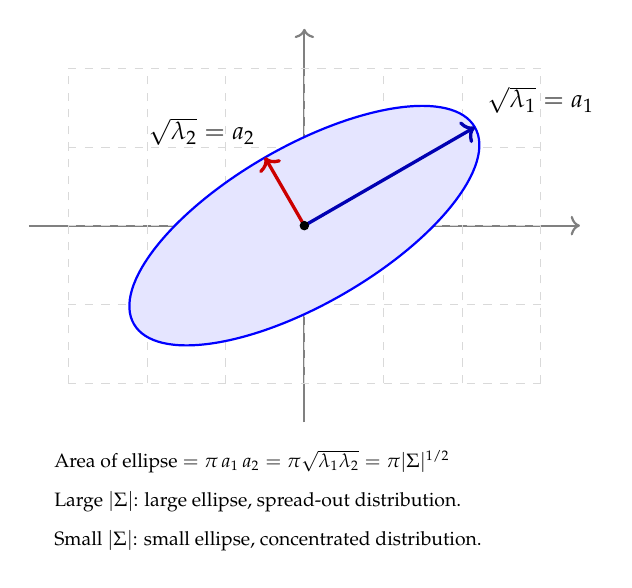
\begin{tikzpicture}[scale=1.0]
    \draw[->, thick, gray] (-3.5,0) -- (3.5,0);
    \draw[->, thick, gray] (0,-2.5) -- (0,2.5);
    \draw[help lines, color=gray!30, dashed] (-3,-2) grid (3,2);
    
    % Mahalanobis ellipse (level set d_M = 1)
    \draw[blue, thick, rotate=30, fill=blue!10] (0,0) ellipse (2.5 and 1);
    
    % Eigenvectors with sqrt(lambda) magnitudes
    \draw[->, thick, blue!70!black, line width=1.2pt] (0,0) -- (2.165, 1.25);
    \node[above right] at (2.2, 1.3) {\small $\sqrt{\lambda_1} = a_1$};
    
    \draw[->, thick, red!80!black, line width=1.2pt] (0,0) -- (-0.5, 0.866);
    \node[above left] at (-0.5, 0.9) {\small $\sqrt{\lambda_2} = a_2$};
    
    \filldraw (0,0) circle (1.5pt);
    
    \node[font=\scriptsize, anchor=west] at (-3.3, -3) 
        {Area of ellipse $= \pi\, a_1\, a_2 = \pi \sqrt{\lambda_1 \lambda_2} = \pi |\Sigma|^{1/2}$};
    \node[font=\scriptsize, anchor=west] at (-3.3, -3.5) 
        {Large $|\Sigma|$: large ellipse, spread-out distribution.};
    \node[font=\scriptsize, anchor=west] at (-3.3, -4) 
        {Small $|\Sigma|$: small ellipse, concentrated distribution.};
\end{tikzpicture}
\caption{The area (volume in 2D) of the Mahalanobis ellipse is
$\pi \sqrt{|\Sigma|}$. The semi-axes are $\sqrt{\lambda_1}$ and
$\sqrt{\lambda_2}$, the square roots of the eigenvalues of $\Sigma$.
The determinant therefore captures the volumetric ``size'' of the
ellipse: a large determinant means a large ellipse, and hence a
distribution that is spread out over a large region of space; a
small determinant means a concentrated distribution.}
\label{fig:volume-ellipsoid}
\end{figure}

\paragraph{The role of $|\Sigma|^{1/2}$ in the density.}
This volumetric interpretation explains why the normalising constant
of the multivariate Gaussian density contains the factor
$|\Sigma|^{1/2}$ in the denominator:
\[
p(x) \;=\; \frac{1}{(2\pi)^{m/2}\, |\Sigma|^{1/2}}\, \exp\!\left(-\tfrac{1}{2}(x-\mu)'\Sigma^{-1}(x-\mu)\right).
\]
The factor $|\Sigma|^{1/2}$ in the denominator is exactly the volume
of the unit Mahalanobis ellipsoid (up to the constant
$(2\pi)^{m/2} / \pi^{m/2} \cdot \Gamma(m/2 + 1)$), which ensures the
density integrates to one. A distribution with a large ellipsoid
(large $|\Sigma|^{1/2}$) must have a low density value at every
point — the probability mass is spread thin. A distribution with a
small ellipsoid (small $|\Sigma|^{1/2}$) is concentrated, and the
density value is correspondingly high.

\paragraph{Why $-\tfrac{1}{2}\log|\Sigma|$ acts as a regulariser.}
Taking the logarithm of the density,
\[
\log p(x) \;=\; -\tfrac{m}{2}\log(2\pi) \;-\; \tfrac{1}{2}\log|\Sigma| \;-\; \tfrac{1}{2}(x-\mu)'\Sigma^{-1}(x-\mu).
\]
The term $-\tfrac{1}{2}\log|\Sigma|$ is a \emph{penalty} that grows
with the volume of the ellipsoid. In the M-step derivations of the
DFM, when we maximise the expected log-likelihood with respect to
$\Sigma$ (whether it is $\mathbf{Q}$ or $\mathbf{R}$), this term
\emph{prevents} the algorithm from making the ellipsoid arbitrarily
large to fit any single observation perfectly. Without the
log-determinant penalty, a degenerate solution with $|\Sigma| \to 0$
in some direction (concentrating all probability mass on a
lower-dimensional subspace) would maximise the kernel term but is
prevented by the divergence of $-\log|\Sigma| \to +\infty$ — an
infinite penalty. The interplay between the kernel
(Mahalanobis-distance) term and the log-determinant term is what
makes the maximum-likelihood estimator of $\Sigma$ well-defined and
non-degenerate.

\newpage

\subsection{Random Matrices and the Circular Law: A Visual Introduction}
\label{sec:appendix-circular-law}

The eigenvalues of a matrix that is constructed from \emph{random}
entries — rather than from data with structure — exhibit a
remarkable regularity. Understanding this regularity provides the
``noise floor'' against which the genuine signal eigenvalues of
empirical covariance matrices must be compared. We give a brief
visual treatment of the Circular Law here; a more formal discussion
can be found in the next section of the appendix.

\paragraph{The Circular Law.}
Let $A_n \in \mathbb{R}^{n \times n}$ be a random matrix whose
entries $A_{n,ij}$ are independent and identically distributed with
mean zero and unit variance. The Circular Law (Ginibre, 1965; Tao
and Vu, 2010) states that, as $n \to \infty$, the eigenvalues of the
\emph{rescaled} matrix $A_n / \sqrt{n}$ converge in distribution to
the uniform distribution on the unit disk in the complex plane:
\[
\big\{\, z \in \mathbb{C} : |z| \leq 1 \,\big\}.
\]
The scaling by $\sqrt{n}$ is essential. Without it, the eigenvalues
would diverge as $n$ grows, scattered ever more wildly across the
complex plane. With the $1/\sqrt{n}$ scaling, the eigenvalues
populate the unit disk uniformly, regardless of the specific
distribution of the entries (only the first two moments matter).

\begin{figure}[H]
\centering
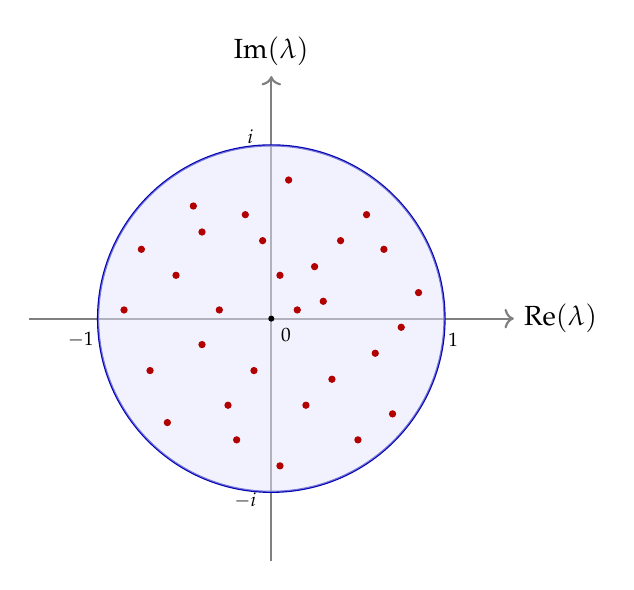
\begin{tikzpicture}[scale=2.2]
    % Real axis
    \draw[->, thick, gray] (-1.4, 0) -- (1.4, 0) node[right, black] {Re$(\lambda)$};
    \draw[->, thick, gray] (0, -1.4) -- (0, 1.4) node[above, black] {Im$(\lambda)$};
    
    % Unit circle
    \draw[blue!70!black, thick] (0,0) circle (1);
    
    % Light blue fill for unit disk
    \fill[blue!10, opacity=0.5] (0,0) circle (1);
    
    % Random eigenvalues scattered inside the disk
    \filldraw[red!70!black] (0.3, 0.1) circle (0.5pt);
    \filldraw[red!70!black] (-0.4, 0.5) circle (0.5pt);
    \filldraw[red!70!black] (0.6, -0.2) circle (0.5pt);
    \filldraw[red!70!black] (-0.7, -0.3) circle (0.5pt);
    \filldraw[red!70!black] (0.1, 0.8) circle (0.5pt);
    \filldraw[red!70!black] (0.55, 0.6) circle (0.5pt);
    \filldraw[red!70!black] (-0.2, -0.7) circle (0.5pt);
    \filldraw[red!70!black] (0.85, 0.15) circle (0.5pt);
    \filldraw[red!70!black] (-0.55, 0.25) circle (0.5pt);
    \filldraw[red!70!black] (0.2, -0.5) circle (0.5pt);
    \filldraw[red!70!black] (-0.3, 0.05) circle (0.5pt);
    \filldraw[red!70!black] (0.4, 0.45) circle (0.5pt);
    \filldraw[red!70!black] (-0.85, 0.05) circle (0.5pt);
    \filldraw[red!70!black] (0.05, -0.85) circle (0.5pt);
    \filldraw[red!70!black] (-0.15, 0.6) circle (0.5pt);
    \filldraw[red!70!black] (0.7, -0.55) circle (0.5pt);
    \filldraw[red!70!black] (-0.6, -0.6) circle (0.5pt);
    \filldraw[red!70!black] (0.25, 0.3) circle (0.5pt);
    \filldraw[red!70!black] (-0.4, -0.15) circle (0.5pt);
    \filldraw[red!70!black] (0.05, 0.25) circle (0.5pt);
    \filldraw[red!70!black] (0.5, -0.7) circle (0.5pt);
    \filldraw[red!70!black] (-0.1, -0.3) circle (0.5pt);
    \filldraw[red!70!black] (0.65, 0.4) circle (0.5pt);
    \filldraw[red!70!black] (-0.45, 0.65) circle (0.5pt);
    \filldraw[red!70!black] (0.35, -0.35) circle (0.5pt);
    \filldraw[red!70!black] (-0.75, 0.4) circle (0.5pt);
    \filldraw[red!70!black] (0.15, 0.05) circle (0.5pt);
    \filldraw[red!70!black] (-0.25, -0.5) circle (0.5pt);
    \filldraw[red!70!black] (0.75, -0.05) circle (0.5pt);
    \filldraw[red!70!black] (-0.05, 0.45) circle (0.5pt);
    
    % Reference points: 1, -1, i, -i
    \node[font=\scriptsize] at (1.05, -0.12) {$1$};
    \node[font=\scriptsize] at (-1.1, -0.12) {$-1$};
    \node[font=\scriptsize] at (-0.12, 1.05) {$i$};
    \node[font=\scriptsize] at (-0.15, -1.05) {$-i$};
    
    \filldraw (0,0) circle (0.4pt);
    \node[font=\scriptsize, below right] at (0,0) {$0$};
    
\end{tikzpicture}
\caption{Eigenvalues of a random matrix $A_n / \sqrt{n}$ in the
complex plane, for $n$ moderately large. The blue circle is the
boundary of the unit disk. As $n \to \infty$, the empirical
distribution of the eigenvalues fills the unit disk uniformly. The
scaling by $\sqrt{n}$ is what places the spectrum on the natural
scale of the unit disk; without this scaling, the eigenvalues would
diverge.}
\label{fig:circular-law}
\end{figure}

\paragraph{Why this matters: the noise floor.}
The Circular Law is the eigenvalue distribution of a matrix with
\emph{no structure} — pure noise. When we apply factor analysis to a
finite sample of macroeconomic data, the empirical covariance matrix
$\widehat{\boldsymbol{\Sigma}}_Y$ contains both signal (from genuine
common factors) and noise (from finite-sample variation in the
idiosyncratic component). The Circular Law characterises the
noise-only contribution: if there were no factors, the eigenvalues
of $\widehat{\boldsymbol{\Sigma}}_Y / \sqrt{n}$ would, in the limit,
be uniformly distributed in the unit disk. Genuine factor
eigenvalues stand out above this noise floor: they appear as
``outliers'' to the bulk of the random-matrix spectrum.

\paragraph{The Marchenko–Pastur companion.}
For the specific case of \emph{symmetric positive semi-definite}
matrices — such as sample covariance matrices computed from $n$
observations of $p$ random variables — the analogue of the Circular
Law is the \emph{Marchenko–Pastur Law} (Marchenko and Pastur,
1967). This result describes the asymptotic distribution of the
eigenvalues of $\widehat{\boldsymbol{\Sigma}}$, when the underlying
population covariance is the identity matrix. The eigenvalues are
no longer uniform on the disk but are distributed on a real interval
$[\lambda_-, \lambda_+]$ with a specific density. The boundary value
$\lambda_+$ provides a sharper estimate of the noise floor for
sample covariance matrices, and is the basis for many modern
factor-selection criteria (such as the Onatski criterion or the
Bai-Ng information criterion).

\paragraph{Bridge to the unit-circle stability condition.}
Beyond providing a noise floor for empirical covariances, the unit
circle in the complex plane plays a second crucial role in the
stability of dynamical systems. We turn to this in the next section.

\newpage 

\subsection{Stability of Linear Dynamical Systems: A Visual Perspective}
\label{sec:appendix-stability-visual}

The unit circle in the complex plane plays two distinct but related
roles in our analysis. First, as we have just seen, it bounds the
``noise floor'' of empirical covariance matrices. Second, it is the
geometric criterion that separates stable from unstable VAR
processes. We now visualise this second role.

\paragraph{Recap: the stability condition.}
Consider a linear dynamical system
\[
x_{t+1} \;=\; \mathbf{A}\, x_t \;+\; u_{t+1}, \qquad t = 0, 1, 2, \ldots
\]
where $\mathbf{A} \in \mathbb{R}^{n \times n}$ is the transition
matrix. As discussed extensively earlier, the process $\{x_t\}$ is
covariance-stationary if and only if all eigenvalues of $\mathbf{A}$
satisfy
\[
|\lambda_i| \;<\; 1, \qquad i = 1, 2, \ldots, n.
\]
Geometrically, all eigenvalues must lie strictly \emph{inside} the
unit circle in the complex plane. Equivalently: the eigenvalues live
in the same set that bounds the noise floor of the Circular Law,
but for a completely different reason.

\paragraph{Three geometric scenarios.}
The position of the eigenvalues in the complex plane immediately
classifies the dynamic behaviour of the process. Three scenarios are
worth visualising side by side.

\begin{figure}[H]
\centering
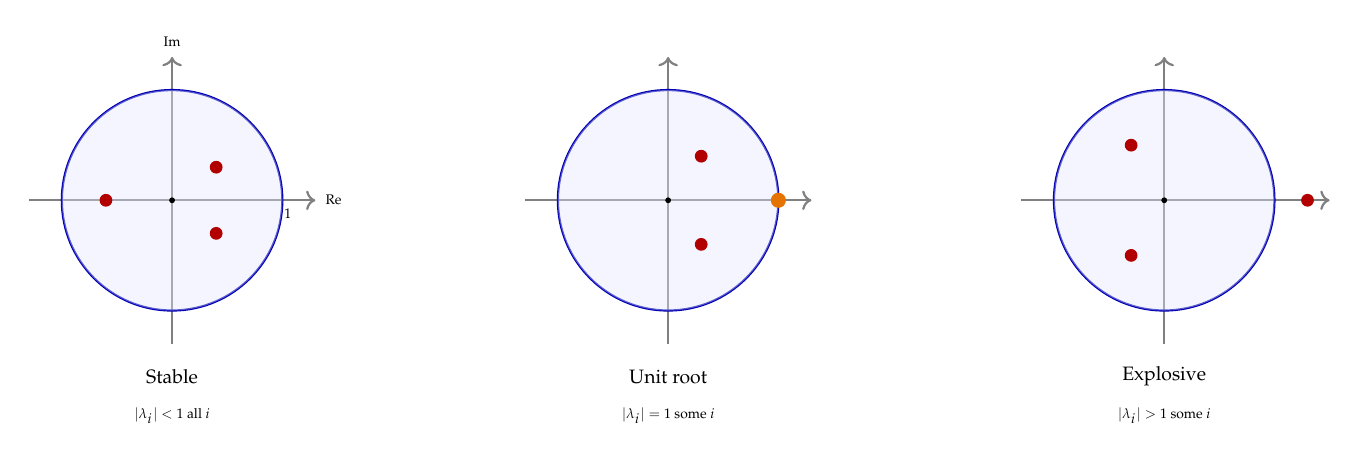
\begin{tikzpicture}[scale=1.4]
    % First panel: stable
    \begin{scope}[shift={(-4.5,0)}]
        \draw[->, thick, gray] (-1.3, 0) -- (1.3, 0) node[right, font=\tiny, black] {Re};
        \draw[->, thick, gray] (0, -1.3) -- (0, 1.3) node[above, font=\tiny, black] {Im};
        \draw[blue!70!black, thick] (0,0) circle (1);
        \fill[blue!10, opacity=0.4] (0,0) circle (1);
        
        % Eigenvalues all inside the circle
        \filldraw[red!70!black] (0.4, 0.3) circle (1.5pt);
        \filldraw[red!70!black] (0.4, -0.3) circle (1.5pt);
        \filldraw[red!70!black] (-0.6, 0) circle (1.5pt);
        
        \filldraw (0,0) circle (0.6pt);
        \node[font=\tiny] at (1.05, -0.12) {$1$};
        \node[font=\scriptsize] at (0, -1.6) {Stable};
        \node[font=\tiny] at (0, -1.95) {$|\lambda_i| < 1$ all $i$};
    \end{scope}
    
    % Second panel: unit root
    \begin{scope}[shift={(0,0)}]
        \draw[->, thick, gray] (-1.3, 0) -- (1.3, 0);
        \draw[->, thick, gray] (0, -1.3) -- (0, 1.3);
        \draw[blue!70!black, thick] (0,0) circle (1);
        \fill[blue!10, opacity=0.4] (0,0) circle (1);
        
        % Two eigenvalues inside, one on the boundary
        \filldraw[red!70!black] (0.3, 0.4) circle (1.5pt);
        \filldraw[red!70!black] (0.3, -0.4) circle (1.5pt);
        \filldraw[orange!90!black] (1, 0) circle (1.8pt);
        
        \filldraw (0,0) circle (0.6pt);
        \node[font=\tiny] at (1.1, -0.15) {};
        \node[font=\scriptsize] at (0, -1.6) {Unit root};
        \node[font=\tiny] at (0, -1.95) {$|\lambda_i| = 1$ some $i$};
    \end{scope}
    
    % Third panel: explosive
    \begin{scope}[shift={(4.5,0)}]
        \draw[->, thick, gray] (-1.3, 0) -- (1.5, 0);
        \draw[->, thick, gray] (0, -1.3) -- (0, 1.3);
        \draw[blue!70!black, thick] (0,0) circle (1);
        \fill[blue!10, opacity=0.4] (0,0) circle (1);
        
        % Two eigenvalues inside, one outside
        \filldraw[red!70!black] (-0.3, 0.5) circle (1.5pt);
        \filldraw[red!70!black] (-0.3, -0.5) circle (1.5pt);
        \filldraw[red!70!black] (1.3, 0) circle (1.5pt);
        
        \filldraw (0,0) circle (0.6pt);
        \node[font=\scriptsize] at (0, -1.6) {Explosive};
        \node[font=\tiny] at (0, -1.95) {$|\lambda_i| > 1$ some $i$};
    \end{scope}
\end{tikzpicture}
\caption{The three regimes of a linear dynamical system, classified
by the position of the eigenvalues of $\mathbf{A}$ in the complex
plane. \emph{Left}: all eigenvalues strictly inside the unit
circle; the process is covariance-stationary, shocks decay
exponentially, the system has a well-defined long-run distribution.
\emph{Middle}: at least one eigenvalue exactly on the unit circle;
the process has a unit root, shocks have permanent effects, and the
variance grows linearly in $t$. \emph{Right}: at least one
eigenvalue outside the unit circle; the process is explosive, shocks
amplify exponentially, the system diverges to infinity.}
\label{fig:unit-circle-stability}
\end{figure}

\paragraph{Why the eigenvalues control everything.}
Recall that the iterated
state at time $t$ depends on $\mathbf{A}^t$ applied to the initial
state. Using the spectral decomposition (when $\mathbf{A}$ is
diagonalisable),
\[
\mathbf{A}^t \;=\; V \Lambda^t V^{-1}, \qquad \Lambda^t = \mathrm{diag}(\lambda_1^t, \ldots, \lambda_n^t).
\]
The behaviour of $\mathbf{A}^t$ is governed by what happens to each
$\lambda_i^t$ as $t$ grows. If $|\lambda_i| < 1$, then $\lambda_i^t \to 0$
exponentially fast — the corresponding mode of the system decays
into oblivion. If $|\lambda_i| = 1$, then $\lambda_i^t$ either
remains constant (real $\lambda_i = 1$) or oscillates (complex
$\lambda_i$ on the unit circle); the mode persists indefinitely. If
$|\lambda_i| > 1$, then $\lambda_i^t \to \infty$ exponentially fast
— the mode amplifies without bound. The eigenvalue \emph{moduli}
control whether each mode dies out, persists, or explodes; the
\emph{arguments} (when complex) control whether each mode oscillates
and at what frequency.

\paragraph{Complex eigenvalues and macroeconomic cycles.}
A pair of complex-conjugate eigenvalues $\lambda = r\, e^{\pm i \theta}$
inside the unit circle ($r < 1$) produces a damped oscillation. The
modulus $r$ controls the rate of damping (closer to $1$ means slower
decay), and the argument $\theta$ controls the frequency (closer to
zero means longer cycles). The corresponding mode of the system
traces an inward spiral in two-dimensional projections, with period
$2\pi/\theta$ and decay rate $r^t$.

This is the algebraic content of business cycles: the cyclical
behaviour observed in macroeconomic data is the geometric expression
of complex eigenvalues of $\mathbf{A}$ that lie inside but not too
close to the origin of the unit disk. After estimation of the DFM,
plotting the eigenvalues of $\widehat{\mathbf{A}}$ in the complex
plane provides a compact diagnostic of both stability (do they lie
inside the unit circle?) and cyclicality (are there complex
eigenvalues close to the boundary, indicating long, slowly damped
cycles?).

\paragraph{Practical implication for the EM algorithm.}
The EM algorithm we use to estimate $\mathbf{A}$ does not impose the
unit-circle constraint during optimisation: each M-step solves the
unconstrained least-squares problem for $\mathbf{A}$. In practice,
when the data have been pre-processed to be stationary
(log-differences, first-differences as appropriate), the estimated
$\widehat{\mathbf{A}}$ at convergence has eigenvalues comfortably
inside the unit circle. Should an estimated eigenvalue approach the
boundary, this is a signal of either insufficient pre-processing or
of a misspecified factor structure that fails to capture all the
non-stationary content of the data.

\paragraph{An equivalent formulation: roots of the characteristic polynomial.}
The reader with a background in classical time-series econometrics
will be familiar with an alternative formulation of the stability
condition. Writing the VAR(1) in lag-operator notation as
\[
(I - \mathbf{A} L)\, x_t \;=\; u_t,
\]
where $L$ is the lag operator, the characteristic polynomial is
$\det(I - \mathbf{A} z) = 0$ for $z \in \mathbb{C}$. The standard
econometric stability condition (Hamilton, 1994; L\"utkepohl, 2005)
requires that all roots $z_i$ of this polynomial lie strictly
\emph{outside} the unit circle:
\[
|z_i| \;>\; 1, \qquad i = 1, 2, \ldots, n.
\]
The two conditions are equivalent. The roots of the characteristic
polynomial are the reciprocals of the eigenvalues of $\mathbf{A}$:
$z_i = 1/\lambda_i$. Therefore $|\lambda_i| < 1$ if and only if
$|z_i| > 1$. Both conditions describe the same geometric fact —
that the system's modes decay rather than amplify over time — but
expressed via different objects: eigenvalues of the transition
matrix (the state-space convention used here) versus roots of the
characteristic polynomial (the classical econometric convention).
We adopt the eigenvalue formulation throughout, in keeping with the
state-space framework that underlies the DFM.

\newpage

\subsection{Matrix Rank: Independent Directions and the Selection Matrix}
\label{sec:appendix-rank}

The final concept we visualise in this appendix is the \emph{rank} of
a matrix. Rank is a notion of ``effective dimensionality'' that
plays a central role in the missing-data formalism we developed
earlier.

\paragraph{Definition.}
The \emph{rank} of a matrix $A \in \mathbb{R}^{m \times n}$ is the
maximum number of linearly independent columns of $A$ — equivalently,
the maximum number of linearly independent rows. Formally,
\[
\mathrm{rank}(A) \;=\; \dim\big(\mathrm{column space of } A\big) \;=\; \dim\big(\mathrm{row space of } A\big).
\]
The rank is bounded above by both $m$ and $n$:
$\mathrm{rank}(A) \leq \min(m, n)$. A matrix is said to have
\emph{full rank} if its rank equals this upper bound, and
\emph{deficient rank} otherwise.

\paragraph{Geometric interpretation.}
The rank of $A$ is the dimension of the image of $T_A$ — the
``effective dimensionality'' of the linear transformation. If
$A \in \mathbb{R}^{m \times n}$ has rank $k$, then the transformation
$T_A: \mathbb{R}^n \to \mathbb{R}^m$ maps every vector in
$\mathbb{R}^n$ into a $k$-dimensional subspace of $\mathbb{R}^m$ —
the column space of $A$. Vectors in $\mathbb{R}^n$ that are mapped
to zero by $T_A$ form the \emph{null space} of $A$, which has
dimension $n - k$ (the rank-nullity theorem).

For a square matrix $A \in \mathbb{R}^{n \times n}$:
\begin{itemize}[leftmargin=1.5em, itemsep=2pt]
    \item $\mathrm{rank}(A) = n$ (full rank): $A$ is invertible,
          $\det(A) \neq 0$, and $T_A$ is a bijection of
          $\mathbb{R}^n$;
    \item $\mathrm{rank}(A) < n$ (rank-deficient): $A$ is singular,
          $\det(A) = 0$, and $T_A$ collapses $\mathbb{R}^n$ to a
          lower-dimensional subspace.
\end{itemize}
This is why the determinant being zero corresponds geometrically to
the volume collapse we visualised previously — a singular matrix has
deficient rank, and its image is a flat, lower-dimensional region.

\paragraph{The selection matrix $\mathbf{W}_t$ as a rank operator.}
The most concrete appearance of rank in our framework is in the
selection matrix $\mathbf{W}_t \in \{0, 1\}^{m_t \times M}$ that
handles missing data. By construction, $\mathbf{W}_t$ has exactly
$m_t$ rows, each of which is a standard basis vector of
$\mathbb{R}^M$ (a row with a single $1$ and the rest zeros). These
rows are linearly independent because they correspond to distinct
basis vectors. Therefore
\[
\mathrm{rank}(\mathbf{W}_t) \;=\; m_t.
\]
The action of $\mathbf{W}_t$ on the full observation vector $y_t$ is
to extract its $m_t$ observed components:
\[
y_t^{\mathrm{obs}} \;=\; \mathbf{W}_t\, y_t \;\in\; \mathbb{R}^{m_t}.
\]
The selection matrix is therefore a \emph{projection} from the
ambient $M$-dimensional observation space to the $m_t$-dimensional
subspace spanned by the currently observed series. As $t$ varies,
the subspace varies — its dimension depends on how many series are
released by time $t$ — but at every $t$ the projection is well-defined
and has rank exactly equal to $m_t$.

\paragraph{Why the rank of $\mathbf{W}_t$ matters.}
Several quantities in the EM derivations depend explicitly on
$m_t = \mathrm{rank}(\mathbf{W}_t)$. Three are especially worth
recalling:
\begin{itemize}[leftmargin=1.5em, itemsep=3pt]
    \item In the weight update for the idiosyncratic shocks,
          \[
          \hat{w}^\varepsilon_t \;=\; \frac{\nu_\varepsilon + m_t}{\nu_\varepsilon + d^{\varepsilon, \mathrm{obs}}_t},
          \]
          the numerator includes $m_t$, the dimension of the
          observed-data space at time $t$. This dimension changes
          across $t$ because of ragged-edge missingness, and the
          weight update correctly reflects the variable amount of
          information available at each $t$.
    \item In the log-likelihood from the Kalman filter,
          \[
          \log p(y_t^{\mathrm{obs}} \mid \theta) \;=\; -\tfrac{1}{2}\big[\log|S_t^{\mathrm{obs}}| + (\eta_t^{\mathrm{obs}})'(S_t^{\mathrm{obs}})^{-1} \eta_t^{\mathrm{obs}} + m_t \log(2\pi)\big],
          \]
          the constant term scales with $m_t$, so periods with fewer
          observations contribute proportionally less to the
          log-likelihood.
    \item In the Mahalanobis distance computed at time $t$, only the
          $m_t \times m_t$ sub-block of $\mathbf{R}$ enters the
          calculation. This sub-block has rank $m_t$ (it is positive
          definite), and the inversion $(\mathbf{W}_t \mathbf{R} \mathbf{W}_t')^{-1}$
          is well-defined precisely because $\mathbf{W}_t$ has full
          row rank.
\end{itemize}
The rank concept is therefore not a mathematical abstraction but a
direct counterpart of the practical question ``how much information
is observable at time $t$?''. The answer is: $m_t$ pieces of
information, encoded by an $m_t$-rank projection from the full
observation space.

\paragraph{Linear dependence and collinearity.}
The most common way for a matrix to fail to have full rank is
\emph{linear dependence} among its columns (or rows). Two vectors
$v_1, v_2 \in \mathbb{R}^n$ are said to be linearly dependent if one
is a scalar multiple of the other, $v_2 = c\, v_1$ for some
$c \in \mathbb{R}$. More generally, a set of vectors
$\{v_1, v_2, \ldots, v_k\}$ is linearly dependent if at least one of
them can be written as a linear combination of the others,
\[
v_k \;=\; c_1 v_1 \;+\; c_2 v_2 \;+\; \cdots \;+\; c_{k-1} v_{k-1},
\]
for some real coefficients $c_1, \ldots, c_{k-1}$. When this happens,
the column space spanned by $\{v_1, \ldots, v_k\}$ has dimension
strictly less than $k$ — the redundant vector $v_k$ adds no new
direction.

In a data matrix $\mathbf{Y} \in \mathbb{R}^{M \times T}$ whose
columns are $T$ observations of $M$ time series, the practical
expression of this phenomenon is \emph{collinearity}: two or more
series move together (up to a scalar) so that one of them is
redundant. If, for instance, two interest rate series are
identical at every $t$, then the corresponding two rows of
$\mathbf{Y}$ are scalar multiples of each other, and
$\mathrm{rank}(\mathbf{Y})$ drops by one. Since for any real matrix
the identity $\mathrm{rank}(\mathbf{Y} \mathbf{Y}') = \mathrm{rank}(\mathbf{Y})$
holds, the sample covariance
$\widehat{\boldsymbol{\Sigma}}_Y = \tfrac{1}{T}\mathbf{Y}\mathbf{Y}'$
inherits the same rank deficiency. By the spectral decomposition,
the number of non-zero eigenvalues of a symmetric matrix equals its
rank — so at least one eigenvalue of
$\widehat{\boldsymbol{\Sigma}}_Y$ is exactly zero. Consequently, the
determinant $|\widehat{\boldsymbol{\Sigma}}_Y| = \prod_i \lambda_i$
is zero, and the matrix is singular: it cannot be inverted, and the
Mahalanobis distance based on it is undefined.

Perfect collinearity rarely occurs in real macroeconomic datasets,
but \emph{near-collinearity} — situations where two or more series
are very highly correlated, though not exactly proportional — is
common. In near-collinearity, the smallest eigenvalues of
$\widehat{\boldsymbol{\Sigma}}_Y$ are not exactly zero but very
close to it. Numerically, this produces an \emph{ill-conditioned}
covariance matrix: $|\widehat{\boldsymbol{\Sigma}}_Y|$ is tiny,
$\widehat{\boldsymbol{\Sigma}}_Y^{-1}$ has very large entries, and
operations involving the inverse (such as the Mahalanobis distance
or the Kalman gain) are numerically unstable. This is one of several
reasons why empirical applications often pre-process data by
selecting representative series within each group, by projecting
onto a smaller number of principal components, or by introducing
explicit regularisation (such as a small ridge $\delta I$ added to
the covariance) to ensure invertibility.

The factor model itself is a structural response to collinearity: by
postulating that $M$ observed series are driven by $r \ll M$ common
factors, the model formalises the empirical observation that
macroeconomic series carry redundant information and admit a
low-dimensional summary. The factor structure replaces the
high-dimensional, near-collinear $\mathbf{Y}$ with a
lower-dimensional, well-conditioned $\mathbf{F}$ that captures the
genuinely independent directions of variation.

\paragraph{Bridge to the formal appendix.}
The visual and intuitive treatment provided in the preceding sections
is intended as preparation for the formal appendix that
follows. The next sections develop the algebraic content: the
spectral theorem proper, the connection between PCA and the
eigendecomposition of the sample covariance, and the explicit
formulae used in the initialisation of the DFM. The geometric
intuitions developed here — vectors as arrows, matrices as
transformations, determinants as volume scaling, eigenvectors as
privileged directions, ellipsoids as level sets, ranks as effective
dimensionalities — are the conceptual scaffolding on which the
algebraic machinery rests.

\newpage
\section{Appendix: Eigenvalues, Eigenvectors, and Principal Components}
\label{sec:appendix-eigen}

This appendix collects the linear algebra used throughout the thesis:
eigenvalues, eigenvectors, the spectral decomposition, their geometric
meaning, their role in characterising stability of linear dynamical
systems, and their role in Principal Component Analysis (PCA). The
material is intended as a reference — the reader who is already
comfortable with these concepts can skip to the summary at the end.
No new results are proved; all statements are classical and can be
found in any graduate-level linear algebra text, for example Horn and
Johnson (2013) or Meyer (2000).

\subsection{Eigenvalues and Eigenvectors: Definition and Intuition}

Let $A \in \mathbb{R}^{n \times n}$ be a square matrix. A non-zero
vector $v \in \mathbb{R}^n$ is called an \emph{eigenvector} of $A$,
with corresponding \emph{eigenvalue} $\lambda \in \mathbb{C}$, if
\begin{equation}
A v \;=\; \lambda\, v.
\label{eq:eigen-definition}
\end{equation}
The defining condition says that $A$ acts on $v$ by simple
\emph{scalar multiplication}: the vector direction is preserved, and
only its magnitude changes, by the factor $\lambda$. Any non-zero
scalar multiple of an eigenvector is itself an eigenvector with the
same eigenvalue, so eigenvectors are naturally thought of as
\emph{directions} rather than as specific vectors; one usually
normalises them to unit length.

\paragraph{The characteristic polynomial.}
Finding eigenvalues reduces to a polynomial-root problem. Rewriting
\eqref{eq:eigen-definition} as $(A - \lambda I) v = 0$, we see that a
non-zero $v$ can satisfy this equation only if the matrix
$A - \lambda I$ is \emph{singular}. Equivalently,
\begin{equation}
\det(A - \lambda I) \;=\; 0.
\label{eq:characteristic-poly}
\end{equation}
The left-hand side, viewed as a function of $\lambda$, is a polynomial
of degree $n$ called the \emph{characteristic polynomial} of $A$. By
the fundamental theorem of algebra, it has exactly $n$ roots in
$\mathbb{C}$ counting multiplicity — so every $n \times n$ matrix has
$n$ eigenvalues (possibly repeated, possibly complex).

\paragraph{Geometric intuition in two dimensions.}
The meaning of the eigenvalue equation is clearest in low dimension.
Consider $A \in \mathbb{R}^{2 \times 2}$ acting on vectors in the
plane. A generic vector $v$ is mapped by $A$ to some new vector $Av$
that is in general \emph{neither} aligned with $v$ nor of the same
length — $A$ both \emph{stretches} and \emph{rotates}. An eigenvector
is a special direction in which the rotation part vanishes: $A$ acts
on an eigenvector by pure stretching, by the factor $\lambda$.

Three illustrative cases in two dimensions sharpen the picture.

\emph{Case 1 — Real positive eigenvalues: pure stretching.} When
$A = \mathrm{diag}(2, 1/2)$, the two eigenvectors are the coordinate
axes, with eigenvalues $2$ and $1/2$. The matrix stretches vectors by
a factor of $2$ along the first axis and compresses them by a factor
of $1/2$ along the second. Applied repeatedly, $A^k$ stretches the
first component geometrically and shrinks the second — the typical
behaviour of a stable system with one dominant direction.

\emph{Case 2 — Real negative eigenvalues: stretching with reflection.}
If $\lambda < 0$, the eigenvector direction is preserved but its
\emph{orientation} is reversed. Applied repeatedly, $A^k$ alternates
sign: oscillation with possible amplification or damping depending on
$|\lambda|$.

\emph{Case 3 — Complex eigenvalues: rotation.} When $A$ is a rotation
matrix or has complex conjugate eigenvalues $\lambda = r e^{\pm i\theta}$,
the eigenvectors are also complex, and $A$ acts on the real plane as
a composition of a rotation by angle $\theta$ and a scaling by $r$.
Applied repeatedly, $A^k$ traces a spiral — inward if $r < 1$,
outward if $r > 1$, and a circle if $r = 1$.

This third case is important: even when $A$ has only real entries,
its eigenvalues can be complex. Complex eigenvalues correspond to
\emph{rotational} or \emph{oscillatory} modes in the dynamics of
repeated multiplication. When we study the stability of a VAR process
below, the complex eigenvalues of the transition matrix capture the
cyclical behaviour of the system.

\subsection{Spectral Decomposition and Symmetric Matrices}

The most important case for our purposes is that of \emph{symmetric}
matrices, which are sufficiently well-behaved to admit a complete
geometric description through eigenvalues and eigenvectors.

\paragraph{The spectral theorem.}
If $A \in \mathbb{R}^{n \times n}$ is symmetric, that is
$A = A^{\top}$, then the spectral theorem guarantees:
\begin{enumerate}[leftmargin=1.5em, itemsep=3pt]
    \item all $n$ eigenvalues of $A$ are real;
    \item there exists an orthonormal basis of $\mathbb{R}^n$
          consisting of eigenvectors of $A$;
    \item $A$ admits the factorisation
          \begin{equation}
          A \;=\; V \Lambda V^{\top},
          \label{eq:spectral-decomposition}
          \end{equation}
          where $V = [v_1, v_2, \ldots, v_n]$ is an orthogonal matrix
          whose columns are the eigenvectors (so $V^{\top} V = I$),
          and $\Lambda = \mathrm{diag}(\lambda_1, \ldots, \lambda_n)$
          is the diagonal matrix of the eigenvalues.
\end{enumerate}
Three consequences of the spectral theorem are used repeatedly.

\paragraph{(i) Geometric reading.}
The factorisation $A = V \Lambda V^{\top}$ reads as a sequence of
three operations on any vector $x$: first, $V^{\top} x$ rotates $x$
into the basis of the eigenvectors; second, $\Lambda V^{\top} x$
stretches each rotated component by the corresponding eigenvalue;
third, $V (\Lambda V^{\top} x)$ rotates back to the original basis.
In other words, $A$ is a \emph{rotation + diagonal stretching +
inverse rotation}. The eigenvectors mark the directions along which
$A$'s action is diagonal; the eigenvalues measure the stretching in
those directions.

\paragraph{(ii) Powers and functions of matrices.}
Once $A = V \Lambda V^{\top}$, powers and general functions of $A$
are trivial to compute:
\[
A^k \;=\; V \Lambda^k V^{\top}, \qquad
f(A) \;=\; V\, f(\Lambda)\, V^{\top},
\]
where $\Lambda^k = \mathrm{diag}(\lambda_1^k, \ldots, \lambda_n^k)$
and $f(\Lambda) = \mathrm{diag}(f(\lambda_1), \ldots, f(\lambda_n))$.
The same logic extends to non-symmetric diagonalisable matrices via
$A^k = V \Lambda^k V^{-1}$ (with $V^{-1}$ in place of $V^{\top}$):
the stability of the iteration $x_{t+1} = A x_t$ is therefore
governed by the eigenvalues of $A$, since the iterated map
$A^k x_0$ amounts to raising each $\lambda_i$ to the $k$-th power.
The unit-circle stability condition $|\lambda_i| < 1$ for the VAR
transition matrix is the direct application of this principle.

\paragraph{(iii) Determinant and trace.}
Since the determinant and trace are invariant under change of basis,
we have
\[
\det(A) \;=\; \prod_{i=1}^{n} \lambda_i, \qquad
\mathrm{tr}(A) \;=\; \sum_{i=1}^{n} \lambda_i.
\]
These identities let us read off two global summaries of $A$'s action
directly from the eigenvalues: the determinant measures the volume
change induced by $A$, and the trace measures the total stretching
along the eigenvector directions.

\subsection{Positive Definite Matrices}

A symmetric matrix $A$ is \emph{positive definite} (PD) if
$x^{\top} A x > 0$ for all $x \neq 0$, and \emph{positive semi-definite}
(PSD) if the inequality is relaxed to $\geq$. The two notions
correspond exactly to sign conditions on the eigenvalues:
\begin{itemize}[leftmargin=1.5em, itemsep=2pt]
    \item $A$ is PD $\iff$ all eigenvalues $\lambda_i > 0$;
    \item $A$ is PSD $\iff$ all eigenvalues $\lambda_i \geq 0$.
\end{itemize}
This follows immediately from the spectral decomposition: writing
$y = V^{\top} x$, the quadratic form $x^{\top} A x = y^{\top} \Lambda y = \sum_i \lambda_i y_i^2$,
which is positive for all $x \neq 0$ precisely when all $\lambda_i > 0$.

\paragraph{Geometric meaning.}
Positive definite symmetric matrices arise naturally as covariance
matrices and as scale matrices of multivariate densities (such as
those of the Gaussian and multivariate Student-$t$). Their level sets
\[
\{x \in \mathbb{R}^n : x^{\top} A^{-1} x \leq c\}
\]
are \emph{ellipsoids} centred at the origin, with axes aligned with
the eigenvectors of $A$ and semi-axis lengths proportional to
$\sqrt{\lambda_i}$. A degenerate case — with one or more eigenvalues
equal to zero — corresponds to an ellipsoid that has collapsed to a
lower-dimensional subspace, geometrically representing a degenerate
distribution. Throughout the DFM estimation, ensuring that the
estimated scale matrices $\hat{\mathbf{Q}}$ and $\hat{\mathbf{R}}$
remain strictly positive definite is a practical concern precisely
because their eigenvalues must not be allowed to approach zero.

\paragraph{The square root of a PD matrix.}
Given a PD matrix $A = V \Lambda V^{\top}$, its \emph{symmetric square
root} is
\[
A^{1/2} \;=\; V \Lambda^{1/2} V^{\top},
\qquad
\Lambda^{1/2} = \mathrm{diag}(\sqrt{\lambda_1}, \ldots, \sqrt{\lambda_n}).
\]
This satisfies $A^{1/2} A^{1/2} = A$ and is used, for example, in the
whitening transformation $z = A^{-1/2}(x - \mu)$ that maps a
multivariate Gaussian $\mathcal{N}(\mu, A)$ to the standard Gaussian
$\mathcal{N}(0, I)$. Only PD matrices admit a real symmetric square
root; this is one of several ways in which positive definiteness is
the algebraic property that makes covariance matrices analytically
tractable.

\subsection{Eigenvalues and the Geometry of Random Matrices}

A final topic worth mentioning is the distribution of eigenvalues of
\emph{random} matrices, which provides useful intuition for finite-sample
behaviour in PCA and factor analysis. The relevant result here is the
Circular Law.

\paragraph{The Circular Law.}
Consider an $n \times n$ matrix $A$ whose entries $A_{ij}$ are
independent and identically distributed random variables with mean
zero and unit variance. The Circular Law (Ginibre, 1965; Tao and Vu,
2010) states that, as $n \to \infty$, the eigenvalues of $A/\sqrt{n}$
converge in distribution to the uniform distribution on the unit disk
in the complex plane: $\{z \in \mathbb{C} : |z| \leq 1\}$.

The scaling by $\sqrt{n}$ is essential — it places the spectrum on a
natural scale. Without it, the eigenvalues of $A$ itself would
diverge as $n$ grows; with it, they populate the complex plane
uniformly inside the unit circle.

\paragraph{Why this matters.}
The Circular Law has two practical consequences relevant to our
setting. First, it describes the ``noise floor'' of empirical
covariance matrices: when we compute the sample covariance of $n$
i.i.d.\ random variables from $T$ observations, the resulting matrix
has eigenvalues that, for large $n$ relative to $T$, populate a
bounded region of the complex plane. Signal eigenvalues (reflecting
true common factors) stand out above this noise floor only if they
are sufficiently large. This intuition is formalised by the
Marchenko-Pastur law (Marchenko and Pastur, 1967), which is the
symmetric-matrix version of the Circular Law — and it underlies many
criteria for selecting the number of factors in large-dimensional
factor models.

Second, the unit circle in the complex plane plays a central role in
the stability analysis of linear dynamical systems: a VAR process is
stationary if and only if the eigenvalues of its transition matrix
lie strictly \emph{inside} the unit circle. This connection is the
subject of the next subsection.

\subsection{Eigenvalues and the Stability of Linear Dynamical Systems}
\label{subsec:eigen-stability}

Consider a linear dynamical system driven by a transition matrix
$A \in \mathbb{R}^{n \times n}$:
\[
x_{t+1} \;=\; A\, x_t \;+\; u_{t+1},
\qquad t = 0, 1, 2, \ldots
\]
where $u_t$ is a zero-mean shock with covariance $\mathbf{Q}$. This is
a VAR(1) process — and it is exactly the law of motion of the factors
$f_t$ in our DFM, with $A = \mathbf{A}$ and $u_t \sim t_{\nu_u}(0, \mathbf{Q})$.
A natural question is: under what conditions does the process $\{x_t\}$
remain bounded over time, and does it admit a well-defined long-run
distribution?

The answer is given by the eigenvalues of $A$ and involves one of the
most important geometric objects in the theory of dynamical systems —
the \emph{unit circle} in the complex plane.

\paragraph{Propagation of shocks through $A^k$.}
Iterating the VAR equation, the state at time $t$ is expressed as
\[
x_t \;=\; A^t x_0 \;+\; \sum_{k=0}^{t-1} A^k u_{t-k}.
\]
The behaviour of the system as $t \to \infty$ is therefore dictated
by the powers $A^k$. Using the spectral decomposition (when $A$ is
diagonalisable),
\[
A^k \;=\; V \Lambda^k V^{-1}, \qquad \Lambda^k = \mathrm{diag}(\lambda_1^k, \ldots, \lambda_n^k).
\]
The matrix $A^k$ grows, shrinks, or oscillates depending entirely on
whether each $|\lambda_i|^k$ grows, shrinks, or stays bounded. The
modulus of each eigenvalue is the critical quantity.

\paragraph{The stability condition: eigenvalues strictly inside the unit circle.}
The VAR(1) process is \emph{stable} — and hence \emph{covariance-stationary}
— if and only if all eigenvalues of $A$ satisfy
\begin{equation}
|\lambda_i| \;<\; 1, \qquad i = 1, 2, \ldots, n.
\label{eq:unit-circle-condition}
\end{equation}
Geometrically, all eigenvalues must lie \emph{strictly inside} the
unit circle in the complex plane:
$\{z \in \mathbb{C} : |z| < 1\}$. When this condition holds,
$|\lambda_i|^k \to 0$ as $k \to \infty$ for every $i$, so the shock
propagated through $A^k$ decays exponentially, the infinite sum
$\sum_{k=0}^\infty A^k \mathbf{Q} (A^{\top})^k$ converges to a
well-defined long-run covariance matrix $\boldsymbol{\Sigma}_\infty$,
and the process has a stationary distribution.

Three regimes emerge from this condition:
\begin{itemize}[leftmargin=1.5em, itemsep=3pt]
    \item \emph{All $|\lambda_i| < 1$: stable}. The process is
          stationary; shocks dissipate exponentially; the factors
          fluctuate around a well-defined mean level (in our case,
          zero, since the factors are centred by construction).
    \item \emph{Some $|\lambda_i| = 1$: unit root}. The process has
          one or more unit roots; shocks have permanent effects, and
          the variance of $x_t$ grows linearly in $t$. This is the
          regime of the integrated processes I(1) — random walks and
          their multivariate generalisations.
    \item \emph{Some $|\lambda_i| > 1$: explosive}. Shocks amplify
          exponentially, and the process diverges to infinity. This
          regime is not economically realistic for macroeconomic
          time series and corresponds to a misspecified model.
\end{itemize}

\paragraph{Why ``strict'' inequality?}
The condition $|\lambda_i| < 1$ must be strict: an eigenvalue
\emph{on} the unit circle gives a unit root and a non-stationary
process. For our DFM, we require all eigenvalues of $\mathbf{A}$ to
lie strictly inside the unit circle so that the estimated factor
process has a stationary distribution and the associated Kalman
filter produces well-defined long-run covariances. In practice, the
EM algorithm we use does not \emph{impose} this constraint during
estimation, but in all applications we verify that the estimated
$\widehat{\mathbf{A}}$ satisfies it. Should an eigenvalue approach
unity during the iteration, this would signal either an integrated
process mistakenly modelled as stationary, or a numerical problem
requiring regularisation.

\paragraph{The connection with pre-processing.}
This is why the stationarity pre-processing discussed at the beginning is essential: we transform each
series (log-differences for real and price variables, first differences
for rates) so that the input to the DFM is stationary. Without this
pre-processing, the common factors extracted from the panel would
inherit non-stationary behaviour, causing one or more eigenvalues of
$\mathbf{A}$ to sit on or near the unit circle, and breaking the
state-space machinery. The unit-circle condition on
$\widehat{\mathbf{A}}$ is, in this sense, the analytical counterpart
of the empirical choice to work with growth rates rather than levels.

\paragraph{Complex eigenvalues and macroeconomic cycles.}
Even in the stable regime, real macroeconomic transition matrices
typically have \emph{complex} eigenvalues. A complex eigenvalue
$\lambda = r e^{i\theta}$ with $r < 1$ produces a damped oscillation:
the impulse response to a shock traces a spiralling path in the
factor space, decaying at rate $r^k$ and cycling with period
$2\pi/\theta$. This is the algebraic expression of the business
cycle: the cyclical pattern in the factors corresponds to complex
eigenvalues of $\mathbf{A}$, with the period determined by their
argument and the damping by their modulus. Plotting the eigenvalues
of $\widehat{\mathbf{A}}$ in the complex plane, after estimation,
provides a compact visualisation of the cyclical content of the
estimated dynamics.

\subsection{Principal Component Analysis}
\label{subsec:pca-theory}

Having established the centrality of eigendecomposition in both the
geometry of covariance matrices and the stability of linear dynamics,
we turn to \emph{Principal Component Analysis} (PCA). PCA is, at its
core, an eigenvalue problem applied to the empirical covariance
matrix. We derive it from first principles and then connect it to
our DFM initialisation.

\paragraph{The problem.}
Let $\mY \in \mathbb{R}^{M \times T}$ be a data matrix whose columns
are $T$ observations of an $M$-dimensional random vector, centred to
have zero sample mean. Define the $M \times M$ sample covariance
matrix
\[
\widehat{\boldsymbol{\Sigma}}_Y \;=\; \frac{1}{T} \mY \mY^{\top}.
\]
PCA seeks a small number $r < M$ of linear combinations of the $M$
series that capture as much of the variability in $\mY$ as possible.
Formally, we seek directions $v_1, v_2, \ldots, v_r \in \mathbb{R}^M$
with $\|v_k\| = 1$ such that the scalar time series
\[
z_{k, t} \;=\; v_k^{\top}\, y_t
\]
have maximal variance, subject to $v_k$ being orthogonal to all
previous directions.

\paragraph{The first principal component.}
The first principal direction $v_1$ is the solution of
\begin{equation}
v_1 \;=\; \argmax_{\|v\| = 1}\; \mathrm{Var}(v^{\top} y_t) \;=\; \argmax_{\|v\| = 1}\; v^{\top} \widehat{\boldsymbol{\Sigma}}_Y\, v.
\label{eq:pca-first-direction}
\end{equation}
This is a constrained quadratic optimisation: maximise the quadratic
form $v^{\top} \widehat{\boldsymbol{\Sigma}}_Y v$ on the unit sphere
$\{v : \|v\| = 1\}$. The Lagrangian is
\[
\mathcal{L}(v, \mu) \;=\; v^{\top} \widehat{\boldsymbol{\Sigma}}_Y\, v \;-\; \mu\,(v^{\top} v - 1),
\]
with first-order condition
$\widehat{\boldsymbol{\Sigma}}_Y\, v = \mu\, v$. This is \emph{exactly}
the eigenvalue equation for $\widehat{\boldsymbol{\Sigma}}_Y$, with
Lagrange multiplier $\mu$ playing the role of the eigenvalue. The
solution is therefore an eigenvector of $\widehat{\boldsymbol{\Sigma}}_Y$,
and at the optimum,
$v_1^{\top} \widehat{\boldsymbol{\Sigma}}_Y\, v_1 = \mu$: the variance
explained by $v_1$ equals its eigenvalue. To maximise the explained
variance, we choose the eigenvector \emph{corresponding to the
largest eigenvalue} $\lambda_1$.

\paragraph{Subsequent principal components.}
The second principal direction $v_2$ is defined by the same
optimisation, with the additional constraint $v_2 \perp v_1$. By the
spectral theorem, the eigenvectors of the symmetric
$\widehat{\boldsymbol{\Sigma}}_Y$ are mutually orthogonal, so the
solution is simply the eigenvector corresponding to the second-largest
eigenvalue $\lambda_2$. More generally, the $k$-th principal direction
$v_k$ is the eigenvector corresponding to the $k$-th largest
eigenvalue $\lambda_k$.

\paragraph{The PCA identity.}
Collecting the eigenvalues in decreasing order
$\lambda_1 \geq \lambda_2 \geq \ldots \geq \lambda_M \geq 0$ (the
inequality $\geq 0$ holds because
$\widehat{\boldsymbol{\Sigma}}_Y$ is positive semi-definite, being a
scaled sum of outer products), and the corresponding eigenvectors
$v_1, \ldots, v_M$ as the columns of an orthogonal matrix $V$, the
spectral decomposition of $\widehat{\boldsymbol{\Sigma}}_Y$ reads
\[
\widehat{\boldsymbol{\Sigma}}_Y \;=\; V\, \Lambda\, V^{\top}, \qquad \Lambda = \mathrm{diag}(\lambda_1, \ldots, \lambda_M).
\]
This is the formal content of PCA: it \emph{is} the eigendecomposition
of the sample covariance matrix. The principal components themselves
are obtained by projecting the data onto the eigenvector basis:
\[
Z \;=\; V^{\top}\, \mY \;\in\; \mathbb{R}^{M \times T},
\]
where the $k$-th row of $Z$ is the $k$-th principal component time
series.

\paragraph{Variance explained and dimensionality reduction.}
The total variance of the data is $\mathrm{tr}(\widehat{\boldsymbol{\Sigma}}_Y) = \sum_k \lambda_k$
(the trace equals the sum of eigenvalues). The fraction of total
variance explained by the first $r$ principal components is therefore
\[
\text{variance explained by } z_1, \ldots, z_r \;=\; \frac{\sum_{k=1}^r \lambda_k}{\sum_{k=1}^M \lambda_k}.
\]
If the spectrum of $\widehat{\boldsymbol{\Sigma}}_Y$ is
\emph{concentrated} — that is, a few large eigenvalues followed by
many small ones — then a small number $r$ of principal components
captures most of the variance, and the data admit a
\emph{low-dimensional summary} in terms of those $r$ components.
This is the empirical foundation of factor modelling: high-dimensional
macroeconomic data typically have a few dominant eigenvalues
corresponding to common factors, and many small eigenvalues
corresponding to idiosyncratic noise. The ``scree plot'' of
eigenvalues in decreasing order — and the identification of the
``elbow'' separating large from small eigenvalues — is the
traditional graphical tool for selecting $r$.

\subsection{PCA as Initialisation for the DFM}
\label{subsec:pca-init}

We now return to the DFM of this thesis and explain why PCA provides
a natural starting point for the EM algorithm — the role of PCA in
the initialisation step.

\paragraph{The intuition.}
The DFM postulates that the $M$ observed series are driven by $r$
common factors through a linear loading matrix $\mL$, plus
idiosyncratic noise:
\[
y_t \;=\; \mL\, f_t \;+\; \varepsilon_t.
\]
If the idiosyncratic component $\varepsilon_t$ is ``small'' relative
to the common component $\mL f_t$, then the covariance of $y_t$ is
dominated by
$\mL\, \mathrm{Var}(f_t)\, \mL^{\top}$ — a rank-$r$ matrix. Its top
$r$ eigenvectors span the same column space as $\mL$, and the
corresponding eigenvalues reflect the variance contributions of the
factors. PCA — which extracts precisely these top eigenvectors from
$\widehat{\boldsymbol{\Sigma}}_Y$ — therefore recovers a basis for
the factor space, up to an orthogonal rotation.

This observation is classical and underlies the equivalence between
PCA and static factor analysis. For our initialisation purposes, PCA
gives us three quantities ``for free'': a basis for the factors (the
top $r$ eigenvectors of
$\widehat{\boldsymbol{\Sigma}}_Y$), starting values for the factor
loadings $\mL^{(0)}$ (read off from the same eigenvectors), and an
initial sense of which directions in data space carry the most
variance.

\paragraph{The standard initialisation procedure.}
Concretely, the initialisation of the DFM proceeds as follows. With
the data balanced
and pre-processed to be centred and unit-variance:
\begin{enumerate}[leftmargin=1.5em, itemsep=3pt]
    \item Form the sample covariance
          $\widehat{\boldsymbol{\Sigma}}_Y = \frac{1}{T} \mY \mY^{\top}$.
    \item Compute its spectral decomposition
          $\widehat{\boldsymbol{\Sigma}}_Y = V \Lambda V^{\top}$,
          with eigenvalues ordered decreasingly
          $\lambda_1 \geq \ldots \geq \lambda_M$.
    \item Retain the top $r$ eigenvectors
          $V_r = [v_1, v_2, \ldots, v_r] \in \mathbb{R}^{M \times r}$.
    \item Set the initial loading matrix to
          $\mL^{(0)} = V_r \Lambda_r^{1/2}$, where
          $\Lambda_r = \mathrm{diag}(\lambda_1, \ldots, \lambda_r)$.
    \item Set the initial factors to
          $\mF^{(0)} = \Lambda_r^{-1/2}\, V_r^{\top}\, \mY$, a
          $r \times T$ matrix whose rows have unit variance and are
          mutually uncorrelated in sample.
\end{enumerate}
With these initialisations in hand, the remaining parameters
$\mA^{(0)}, \mQ^{(0)}, \mR^{(0)}$ are obtained from ordinary least
squares applied to the PCA factors, and the degrees of freedom are
initialised at $\nu_u^{(0)} = \nu_\varepsilon^{(0)} = 10$ as discussed previously. The EM iteration then
takes over.

\paragraph{Why PCA initialisation works in practice.}
PCA is an \emph{approximation} to the correct initialisation for the
DFM, not the exact solution. Three approximations are made:
\begin{itemize}[leftmargin=1.5em, itemsep=3pt]
    \item \emph{Static rather than dynamic.} PCA extracts factors
          from a \emph{static} covariance, ignoring the VAR dynamics
          of $f_t$ specified in the model. The true factor estimator
          should account for $\mA$ and the time structure.
    \item \emph{Gaussian rather than heavy-tailed.} PCA assumes
          Gaussian errors implicitly (least-squares projection); the
          Student-$t$ structure of our model is ignored at this
          stage.
    \item \emph{Equal-weight over time.} PCA weights every observation
          equally; the correct weighting in the Student-$t$ framework
          would use the posterior weights $\hat{w}^u_t, \hat{w}^\varepsilon_t$.
\end{itemize}
Despite these approximations, PCA produces a starting point that is
\emph{close enough} to the true optimum that the EM algorithm
converges within 50--200 iterations in typical applications. The
EM iteration itself corrects for each of the three approximations:
the Kalman filter introduces the dynamic structure, the posterior
weights introduce the correct Student-$t$ down-weighting, and the
M-step updates realign the parameters with all of these refinements.
The role of PCA is therefore not to provide a final answer, but to
provide a \emph{good enough starting point} from which the EM
iteration can descend — or, more precisely, ascend — to the
maximum-likelihood estimate efficiently.

\paragraph{Eigenvalue inspection during estimation.}
Beyond initialisation, the eigenvalues of
$\widehat{\boldsymbol{\Sigma}}_Y$ are a useful diagnostic throughout.
The scree plot of the eigenvalues — or, equivalently, the ``variance
explained'' curve — helps confirm that the chosen number of factors
$r$ is appropriate: ideally, $\lambda_1, \ldots, \lambda_r$ should
stand clearly above $\lambda_{r+1}, \lambda_{r+2}, \ldots$. If there
is no clear separation, this is a signal that either $r$ is
mis-specified, or that the signal-to-noise ratio in the data is too
low for reliable factor extraction. Such diagnostics are standard in
applied factor modelling and inform our choice of $r$ in the
empirical work.

\subsection{Summary: Eigenvalues in the DFM Pipeline}

We close this appendix by collecting, in a single place, the distinct
roles played by eigenvalues and eigenvectors throughout the DFM
estimation.

\paragraph{Covariance and scale matrices: positive definite structure.}
The innovation covariance $\mathbf{Q}$, the idiosyncratic scale
$\mathbf{R}$, and the posterior covariances
$\tilde{P}_{t \mid T}$ produced by the Kalman smoother are all
symmetric positive definite. Their positive eigenvalues ensure that
the Mahalanobis distances, quadratic forms, and log-determinants
appearing in the EM derivations are well-defined. A numerical
collapse of any eigenvalue toward zero signals that the estimation is
producing a degenerate distribution and requires regularisation.

\paragraph{Transition matrix: stability via the unit circle.}
The VAR transition matrix $\mathbf{A}$ governs the dynamic stability
of the factor process. Its eigenvalues must lie strictly inside the
unit circle for the process to be stationary and for the Kalman
filter to produce bounded long-run covariances. The modulus of each
eigenvalue measures persistence; complex eigenvalues correspond to
cyclical modes. After estimation, the spectrum of
$\widehat{\mathbf{A}}$ is inspected to confirm stability and to
interpret the cyclical content of the estimated dynamics.

\paragraph{Data covariance: PCA initialisation.}
The sample covariance
$\widehat{\boldsymbol{\Sigma}}_Y$ admits a spectral decomposition
whose top $r$ eigenvectors provide initial values for the factor
loadings, and whose top eigenvalues measure the variance captured by
each initial factor. PCA is the algebraic expression of ``find the
directions of maximal variance'', and these directions are, in turn,
the eigenvectors of the covariance. The EM algorithm corrects the
approximations inherent in this starting point through iterated
Kalman filtering and M-step updates.

\paragraph{Random matrices: noise-floor intuition.}
The Circular Law and its relatives (the Marchenko-Pastur law in
particular) characterise the distribution of eigenvalues of empirical
covariance matrices in the absence of a true signal. They provide a
``noise floor'' against which genuine factor eigenvalues must stand
out for the DFM to extract meaningful structure. While we do not use
these results formally in estimation, they provide the theoretical
backdrop against which choices such as the number of factors $r$
must be made.

In sum: eigenvalues quantify stability, dispersion, and information
content; eigenvectors identify principal directions, factor
loadings, and modes of dynamics. The repeated appearance of
eigendecomposition in the DFM pipeline is not a coincidence but the
algebraic expression of the fact that multivariate linear models are
best understood in the basis that diagonalises their fundamental
operators.


\end{document}